% Medorama: User's manual.
% Built with pdflatex (latexmk, or Overleaf: see README.md). The source is ASCII: special
% characters are written as LaTeX commands. Every change to Medorama is reflected here, in the
% same change as the code and the Markdown documents.
%
% Chapters and their labels (refer to them with \cref{chap:...}):
%   Part I    introduction (chap:introduction), installation (chap:installation),
%             quickstart (chap:quickstart)
%   Part II   page (chap:page), patients (chap:patients), cohorts (chap:cohorts),
%             databases-tab (chap:databases-tab), viewers-in-medorama (chap:viewers-in-medorama),
%             actions (chap:actions)
%   Part III  importing (chap:importing), connecting (chap:connecting), clif (chap:clif),
%             recordings (chap:recordings), ecg-imaging (chap:ecg-imaging)
%   Part IV   viewers-alone (chap:viewers-alone), vitalstream (chap:vitalstream),
%             ecg-viewer (chap:ecg-viewer), pacs-viewer (chap:pacs-viewer)
%   Part V    administration (chap:administration), users-privacy (chap:users-privacy),
%             sign-in (chap:sign-in), deployment (chap:deployment), addons (chap:addons),
%             readers (chap:readers), troubleshooting (chap:troubleshooting)
%   Part VI   architecture (chap:architecture), protecting (chap:protecting),
%             security (chap:security): for an institution's IT security review
%   Part VII  cli (chap:cli), http-api (chap:http-api), viewer-api (chap:viewer-api),
%             settings-reference (chap:settings-reference), formats-reference (chap:formats-reference)
%   Appendices  app-glossary (chap:glossary), app-licences (chap:licences)
% A section's label is sec:<chapter>-<topic>, a table's tab:<chapter>-<topic>, a figure's
% fig:<chapter>-<topic>: each chapter's labels start with its own name, so that none repeat.
\documentclass[11pt,a4paper,oneside,openany]{book}
% Preamble of the Medorama user's manual (medorama-user-manual.tex); the design of the WFDB-x
% manual's, so that the two read alike.
% Built with pdflatex (latexmk; see README.md). The source is ASCII: special characters are
% written as LaTeX commands.

% ---- Engine, encoding and fonts ----------------------------------------------------------
\usepackage{iftex}
\ifPDFTeX
  \usepackage[T1]{fontenc}
  \usepackage[utf8]{inputenc}
\else
  \usepackage{fontspec}
\fi
\usepackage{XCharter}                               % text: Charter
\IfFileExists{sourcesans.sty}                       % headings, labels: Source Sans (\sffamily)
  {\usepackage{sourcesans}}{\usepackage{sourcesanspro}}  % (older TeX distributions)
\usepackage[varqu,varl,scaled=0.9]{zi4}             % code: Inconsolata, upright quotes, bold
\usepackage{textcomp}
\usepackage{amsmath,amssymb}
\usepackage{microtype}
\DisableLigatures[-,<,>]{family=tt*}           % "--", "<<", ">>" stay as typed in code

% ---- Colors (color-blind-safe; red is never used: it is reserved for alarms) --------------------
\usepackage[table]{xcolor}
\definecolor{titlecolor}{HTML}{12324A}               % headings, title page
\definecolor{accent}{HTML}{0072B2}                   % Okabe-Ito blue: numbers, links, rules
\definecolor{okskyblue}{HTML}{56B4E9}
\definecolor{okgreen}{HTML}{009E73}
\definecolor{okorange}{HTML}{E69F00}
\definecolor{okviolet}{HTML}{7B3294}                 % identifying data (PHI)
\definecolor{rulecolor}{HTML}{B8C4CE}
\definecolor{mutedtext}{HTML}{5A6B7B}
\definecolor{codebg}{HTML}{F5F7F9}
\definecolor{codecomment}{HTML}{5A6B7B}
\definecolor{codekeyword}{HTML}{005A8C}
\definecolor{codestring}{HTML}{00785A}
\definecolor{noteback}{HTML}{EBF4FA}
\definecolor{phiback}{HTML}{F4EDF8}
\definecolor{tipback}{HTML}{E9F6F1}
\definecolor{tableheadback}{HTML}{EEF2F5}

% ---- Page --------------------------------------------------------------------------------
\usepackage[a4paper,top=28mm,bottom=27mm,inner=27mm,outer=25mm,headheight=15pt,
  headsep=9mm,footskip=11mm]{geometry}
\usepackage[skip=0.55em plus 0.2em minus 0.1em]{parskip}
\raggedbottom
\clubpenalty=10000
\widowpenalty=10000
\setcounter{tocdepth}{2}
\setcounter{secnumdepth}{3}

% ---- Headings and the table of contents --------------------------------------------------
\usepackage{titlesec}
\usepackage{titletoc}
\titleformat{\part}[display]
  {\normalfont\sffamily\centering\color{titlecolor}}
  {\large\bfseries\color{accent}\MakeUppercase{\partname}\enspace\thepart}
  {14pt}
  {\Huge\bfseries}
\titleformat{\chapter}[display]
  {\normalfont\sffamily\color{titlecolor}}
  {\large\bfseries\color{accent}\MakeUppercase{\chaptertitlename}\enspace\thechapter}
  {4pt}
  {{\color{accent}\titlerule[1.2pt]}\vspace{10pt}\Huge\bfseries}
\titleformat{name=\chapter,numberless}[display]
  {\normalfont\sffamily\color{titlecolor}}
  {}
  {0pt}
  {{\color{accent}\titlerule[1.2pt]}\vspace{10pt}\Huge\bfseries}
\titlespacing*{\chapter}{0pt}{0pt}{26pt}
\titleformat{\section}
  {\normalfont\sffamily\Large\bfseries\color{titlecolor}}{\color{accent}\thesection}{0.75em}{}
\titleformat{\subsection}
  {\normalfont\sffamily\large\bfseries\color{titlecolor}}{\color{accent}\thesubsection}{0.75em}{}
\titleformat{\subsubsection}
  {\normalfont\sffamily\normalsize\bfseries\color{titlecolor}}{\thesubsubsection}{0.75em}{}
\titleformat{\paragraph}[runin]
  {\normalfont\sffamily\normalsize\bfseries\color{titlecolor}}{}{0pt}{}
\titlespacing*{\section}{0pt}{1.6em plus 0.4em minus 0.2em}{0.5em}
\titlespacing*{\subsection}{0pt}{1.3em plus 0.3em minus 0.2em}{0.4em}
\titlespacing*{\subsubsection}{0pt}{1.1em plus 0.3em minus 0.2em}{0.3em}
\titlespacing*{\paragraph}{0pt}{0.8em plus 0.2em}{0.6em}

\titlecontents{part}[0pt]
  {\addvspace{1.3em}\sffamily\bfseries\large\color{titlecolor}}
  {\partname\ \thecontentslabel\quad}{}{\hfill\contentspage}[\addvspace{0.3em}]
\titlecontents{chapter}[2.2em]
  {\addvspace{0.55em}\sffamily\bfseries}
  {\contentslabel{2.2em}}{\hspace*{-2.2em}}{\hfill\contentspage}
\titlecontents{section}[4.9em]
  {\small}{\contentslabel{2.7em}}{\hspace*{-2.7em}}
  {\titlerule*[0.7pc]{.}\contentspage}
\titlecontents{subsection}[8.4em]
  {\small\color{mutedtext}}{\contentslabel{3.5em}}{\hspace*{-3.5em}}
  {\titlerule*[0.7pc]{.}\contentspage}
\titlecontents{figure}[2.6em]
  {\small}{\contentslabel{2.6em}}{\hspace*{-2.6em}}{\titlerule*[0.7pc]{.}\contentspage}

% ---- Running heads -----------------------------------------------------------------------
\usepackage{fancyhdr}
\pagestyle{fancy}
\fancyhf{}
\fancyhead[L]{\sffamily\small\color{mutedtext}\nouppercase{\leftmark}}
\fancyhead[R]{\sffamily\small\bfseries\color{titlecolor}\thepage}
\fancyfoot[L]{\sffamily\footnotesize\color{mutedtext}Medorama\enspace\textbar\enspace
  User's manual}
\fancyfoot[R]{\sffamily\footnotesize\color{mutedtext}Version \mdversion}
\renewcommand{\headrule}{{\color{rulecolor}\hrule height 0.4pt width\headwidth}}
\renewcommand{\footrulewidth}{0pt}
\renewcommand{\chaptermark}[1]{\markboth{%
  \ifnum\value{secnumdepth}>-1 \ifnum\value{chapter}>0 \thechapter\quad\fi\fi #1}{}}
\fancypagestyle{plain}{\fancyhf{}%
  \fancyfoot[L]{\sffamily\footnotesize\color{mutedtext}Medorama\enspace\textbar\enspace
    User's manual}%
  \fancyfoot[R]{\sffamily\footnotesize\bfseries\color{titlecolor}\thepage}%
  \renewcommand{\headrulewidth}{0pt}}

% ---- Lists, figures, tables --------------------------------------------------------------
\usepackage{enumitem}
\setlist{itemsep=0.15em,topsep=0.3em,parsep=0.1em}
\setlist[itemize,1]{label={\color{accent}\textbullet}}
\usepackage{graphicx}
\usepackage{caption}
\captionsetup{font=small,labelfont={bf,sf,color=accent},textfont=sf,labelsep=quad,
  skip=6pt}
\captionsetup[table]{position=top}
\usepackage{float}
\usepackage{booktabs}
\usepackage{array}
\usepackage{tabularx}
\usepackage{longtable}
\usepackage{xltabular}
\usepackage{multirow}
\usepackage{etoolbox}
\newcolumntype{L}{>{\raggedright\arraybackslash}X}       % ragged-right X column
\newcolumntype{P}[1]{>{\raggedright\arraybackslash}p{#1}} % ragged-right fixed-width column
\renewcommand{\arraystretch}{1.2}
\setlength{\aboverulesep}{0.5ex}
\setlength{\belowrulesep}{0.6ex}
\setlength{\heavyrulewidth}{0.9pt}
\setlength{\lightrulewidth}{0.45pt}
\AtBeginEnvironment{tabularx}{\small}
\AtBeginEnvironment{xltabular}{\small}
\newcommand{\tabhead}{\leavevmode\sffamily\bfseries\color{titlecolor}}   % the header cells of a table

% ---- Code --------------------------------------------------------------------------------
\usepackage{listings}
\lstdefinelanguage{Rust}{
  morekeywords={as,break,const,continue,crate,else,enum,extern,false,fn,for,if,impl,in,let,
    loop,match,mod,move,mut,pub,ref,return,self,Self,static,struct,super,trait,true,type,
    unsafe,use,where,while,dyn,Some,None,Ok,Err,Option,Result,Vec,String,u8,u16,u32,u64,
    i16,i32,i64,f32,f64,usize,isize,bool,str},
  sensitive=true,
  morecomment=[l]{//},
  morecomment=[s]{/*}{*/},
  morestring=[b]",
}
\lstdefinelanguage{TOML}{
  morecomment=[l]{\#},
  morestring=[b]",
  morestring=[b]',
  morekeywords={true,false},
}
\lstdefinelanguage{CMake}{
  morekeywords={add_subdirectory,target_link_libraries,set,cmake_minimum_required,project,
    add_executable,find_package,PRIVATE,PUBLIC,CACHE,BOOL,FORCE,OFF,ON,EXCLUDE_FROM_ALL},
  sensitive=false,
  morecomment=[l]{\#},
  morestring=[b]",
}
\lstdefinelanguage{JavaScript}{
  morekeywords={async,await,break,case,catch,const,continue,default,delete,do,else,export,
    false,finally,for,function,if,import,in,instanceof,let,new,null,return,switch,this,throw,
    true,try,typeof,undefined,var,while},
  sensitive=true,
  morecomment=[l]{//},
  morecomment=[s]{/*}{*/},
  morestring=[b]",
  morestring=[b]',
  morestring=[b]`,
}
\lstdefinelanguage{PowerShell}{
  morekeywords={param,if,else,foreach,function,return,try,catch,finally,throw},
  sensitive=false,
  morecomment=[l]{\#},
  morestring=[b]",
  morestring=[b]',
}
\lstdefinelanguage{CSV}{}
\lstdefinelanguage{JSON}{
  morestring=[b]",
  morekeywords={true,false,null},
}
\lstset{
  basicstyle=\ttfamily\small,
  columns=fullflexible,
  keepspaces=true,
  upquote=true,
  showstringspaces=false,
  breaklines=true,
  breakatwhitespace=false,
  postbreak=\mbox{\textcolor{codecomment}{$\hookrightarrow$}\space},
  backgroundcolor=\color{codebg},
  frame=l,
  framerule=2pt,
  rulecolor=\color{okskyblue},
  framesep=6pt,
  xleftmargin=8pt,
  xrightmargin=0pt,
  aboveskip=0.8em,
  belowskip=0.6em,
  tabsize=4,
  keywordstyle=\color{codekeyword}\bfseries,
  commentstyle=\color{codecomment}\itshape,
  stringstyle=\color{codestring},
}
\lstdefinestyle{text}{language={},keywordstyle={},commentstyle={},stringstyle={}}
% The styles of the listings: "signature" is the syntax of a command or a request (one listing
% right after each \apientry), "example" an example, "shell" a command line.
\lstdefinestyle{signature}{backgroundcolor=\color{white},rulecolor=\color{accent},
  basicstyle=\ttfamily\small\bfseries,keywordstyle=\color{codekeyword}}
\lstdefinestyle{example}{}
\lstdefinestyle{shell}{language=bash,keywordstyle={},commentstyle=\color{codecomment},
  stringstyle={}}

% ---- Boxes -------------------------------------------------------------------------------
\usepackage{tikz}
\usepackage[most]{tcolorbox}
\tcbset{mdbox/.style={enhanced,breakable,boxrule=0pt,leftrule=3pt,arc=0pt,outer arc=0pt,
  left=8pt,right=8pt,top=5pt,bottom=5pt,before skip=0.8em,after skip=0.8em,
  fonttitle=\sffamily\bfseries\small,attach title to upper={\quad}}}
\newtcolorbox{note}[1][Note]{mdbox,colback=noteback,colframe=accent,coltitle=accent,
  title={#1}}
\newtcolorbox{tip}[1][Tip]{mdbox,colback=tipback,colframe=okgreen,coltitle=okgreen,
  title={#1}}
\newtcolorbox{phibox}[1][Patient data]{mdbox,colback=phiback,colframe=okviolet,
  coltitle=okviolet,title={#1}}

% ---- Links and references ----------------------------------------------------------------
\usepackage{xurl}
\usepackage[bookmarksnumbered,bookmarksopen,bookmarksopenlevel=0]{hyperref}
\hypersetup{colorlinks=true,linkcolor=accent,urlcolor=accent,citecolor=accent,
  pdftitle={Medorama: User's manual},
  pdfauthor={Reza Sameni},
  pdfsubject={A unified patient-journey research platform linking EHR data, physiological
    waveforms, imaging and laboratory results across databases},
  pdfkeywords={Medorama, VitalStream, patient journey, cohorts, OMOP, CLIF, WFDB, ECG, DICOM,
    privacy, de-identification}}
\usepackage[nameinlink,capitalise,noabbrev]{cleveref}

% ---- Manual macros -----------------------------------------------------------------------
\newcommand{\mdversion}{0.1.0}        % the version of Medorama described
\newcommand{\mddate}{November 2026}
\newcommand{\md}{Medorama}
\newcommand{\ui}[1]{\textsf{\bfseries #1}}   % a button, tab or menu of a page: \ui{Open record\dots}
\newcommand{\key}[1]{\fbox{\footnotesize\sffamily #1}}  % a key of the keyboard

% An underscore that allows a line break after it, so long identifiers wrap in tables.
\DeclareRobustCommand{\_}{\ifmmode\text{\textunderscore}\else\textunderscore\allowbreak\fi}

\newcommand{\code}[1]{\texttt{#1}}          % inline code, identifiers, values (escape _ # % & { })
\newcommand{\cmd}[1]{\texttt{#1}}           % a command line or a subcommand
\newcommand{\opt}[1]{\texttt{#1}}           % a command-line option
% A file or folder of the repository or an output: may break after each /.
\makeatletter
\DeclareRobustCommand{\file}[1]{\texttt{\md@file#1/\@nil}}
\def\md@file#1/#2\@nil{#1\if\relax\detokenize{#2}\relax\else/\allowbreak\md@file#2\@nil\fi}
\makeatother
\newcommand{\phimark}{\textsuperscript{\textcolor{okviolet}{\sffamily\bfseries PHI}}}
\pdfstringdefDisableCommands{\def\_{\textunderscore}\def\allowbreak{}\def\code#1{#1}%
  \def\file#1{#1}\def\cmd#1{#1}\def\opt#1{#1}\def\phimark{}\def\ui#1{#1}\def\key#1{#1}}

% A function or command entry of a reference chapter: \apientry{name}{one-line summary}
\newcommand{\apientry}[2]{\par\addvspace{0.9em}\noindent
  {\color{rulecolor}\rule{\linewidth}{0.4pt}}\par\nopagebreak\vspace{0.15em}\noindent
  {\large\ttfamily\bfseries\color{titlecolor}#1}\hfill{\small\sffamily\color{mutedtext}#2}\par
  \nopagebreak\smallskip}
% Parameter lists of reference entries: \begin{params} \item[\code{name}] meaning \end{params}
\newlist{params}{description}{1}
\setlist[params]{font=\normalfont\ttfamily\bfseries,leftmargin=2.2em,style=nextline,
  itemsep=0.1em}

% Return value and errors of a reference entry: \returns{...} \raises{...}
\newcommand{\returns}[1]{\par\noindent{\sffamily\bfseries\small\color{titlecolor}Returns}
  \quad #1\par}
\newcommand{\raises}[1]{\par\noindent{\sffamily\bfseries\small\color{titlecolor}Errors}
  \quad #1\par}
% Screenshots: \screenshot{file in ../images/screens}{caption}{label}
\graphicspath{{figures/}}   % copies of ../images (screens, diagrams as PDF): make figures
\newcommand{\screenshot}[3]{\begin{figure}[htbp]\centering
  \includegraphics[width=\linewidth,height=0.42\textheight,keepaspectratio]{#1}
  \caption{#2}\label{#3}\end{figure}}



\begin{document}

% ---- Title page --------------------------------------------------------------------------
\begin{titlepage}
  \thispagestyle{empty}
  \vspace*{0.18\textheight}
  {\sffamily\color{accent}\large\bfseries USER'S MANUAL\par}
  \vspace{0.6em}
  {\color{accent}\rule{\linewidth}{1.2pt}\par}
  \vspace{1.0em}
  {\sffamily\bfseries\color{titlecolor}\fontsize{40}{44}\selectfont Medorama\par}
  \vspace{0.8em}
  {\sffamily\Large\color{titlecolor}A unified patient-journey research platform linking EHR
    data, physiological waveforms, imaging and laboratory results across databases\par}
  \vspace{2.2em}
  {\sffamily\large\color{mutedtext}Version \mdversion\quad\textbar\quad \mddate\par}
  \vfill
  {\sffamily\large\color{titlecolor}Reza Sameni\par}
  \vspace{0.3em}
  {\sffamily\small\color{mutedtext}\url{https://medorama.org}\par}
  {\sffamily\small\color{mutedtext}\url{https://github.com/alphanumericslab/medorama}\par}
  \vspace{1.2em}
  {\small\color{mutedtext}
  Medorama is research software, not a medical device: it is not cleared for diagnosis or
  treatment and must not be used to make clinical decisions. Every patient, value, signal and
  image in this manual is synthetic. Licenses: \cref{chap:licences}.\par}
\end{titlepage}

\frontmatter
\tableofcontents
\listoffigures

\mainmatter

% ---- Part I ------------------------------------------------------------------------------
\part{Getting started}
\label{part:start}
\chapter{Introduction}
\label{chap:introduction}

This chapter introduces Medorama: what it does, the programs it is made of, how it protects
patients' identities, the synthetic data used in this manual, and how the manual is organized.

Medorama is a unified patient-journey research platform linking EHR data, physiological
waveforms, imaging and laboratory results across databases, free for noncommercial use. It
brings together what is known about a patient from many sources: admissions and bed stays, laboratory results, vital
signs, medications, conditions, notes, ECGs, imaging and bedside-monitor recordings. Every
patient has a page with their \emph{Patient Journey}, a picture of the whole history with one
column per clinical category, beside a searchable report of every entry. Researchers build
\emph{cohorts} across every database, with criteria written as expressions such as
\code{QTc > 470ms AND female}. Recordings, ECGs, echo loops and images open in Medorama's own
viewers, as tabs of the same page.

\emph{Privacy Mode}, the default for every user except administrators with the PHI permission,
shows the same data without any identifier: the server replaces names and numbers with
placeholders and pseudonyms, moves dates back, and de-identifies files before they leave it.

\screenshot{patient.png}{A patient's page in the dark theme: the Patient Journey (center), the
report and the detail of a 12-lead ECG (right). Synthetic data.}{fig:introduction-patient}

\begin{note}[Research use only]
Medorama is research software, not a medical device: it is not cleared for diagnosis or
treatment, and must not be used to make clinical decisions.
\end{note}

\section{What Medorama does}
\label{sec:introduction-what}

\Cref{tab:introduction-features} summarizes what Medorama offers; each line is a chapter of
\cref{part:using} or \cref{part:data}.

\begin{table}[htbp]
\caption{What Medorama does.}
\label{tab:introduction-features}
\begin{tabularx}{\linewidth}{@{}P{2.9cm}L@{}}
\toprule
{\tabhead Feature} & {\tabhead What it is} \\
\midrule
Cohorts & Patients found across every database by criteria (results, vital signs, ECG and
  imaging measurements, diagnoses, medications, encounters and ICU stays, age, sex, text),
  written as expressions or chosen line by line; kept, refreshed, combined, cloned and shared;
  each cohort's definition records its criteria and every patient added manually; members and
  their data exported as CSV and Excel (\cref{chap:cohorts}). \\
Patient Catalog & Every patient, searchable; each one's page: identity and allergies,
  encounters, medications and conditions, the Patient Journey, a report of every entry
  searchable down to the notes, the detail of each entry (\cref{chap:patients}). \\
Databases & Every imported database as a table, as it was imported, each row linked to its
  patient and its file to its viewer; connected databases (an OMOP CDM instance, a research
  warehouse) read in place, their persons linked to the same patients
  (\cref{chap:databases-tab}). \\
Viewers & VitalStream for ICU monitoring, Holter, EEG and sleep recordings, from weeks down
  to single samples; the ECG viewer, on standard paper; the PACS viewer, for DICOM studies (echo and
  angiography loops, CT, MR, nuclear medicine, X-ray, structured reports)
  (\cref{chap:viewers-in-medorama}). \\
Privacy Mode & Pseudonyms and placeholders instead of identifiers, dates moved back with
  intervals kept, de-identified WFDB, MUSE, DICOM and EDF headers; enforced by the server
  (\cref{sec:introduction-privacy}, \cref{chap:protecting}). \\
Sign-in & Medorama's own accounts and passwords, or the institution's sign-in (single sign-on,
  multi-factor authentication) through an authenticating proxy (\cref{chap:sign-in}). \\
Work & Background indexing, a Holter's heart rate, plug-in actions on any selection of
  recordings (\cref{chap:actions}); users, roles and a separate PHI permission; a sealed
  audit log (\cref{chap:administration}). \\
Scale & SQLite on one server, or PostgreSQL for several servers and many users, with the
  same program (\cref{chap:deployment}). \\
\bottomrule
\end{tabularx}
\end{table}

\section{The parts}
\label{sec:introduction-parts}

Medorama is made of separate programs, each in its own folder of the repository, joined by
written contracts: a file format, an HTTP API, a command-line protocol, an address or a folder
layout. \Cref{tab:introduction-parts} lists them, and \cref{chap:architecture} describes how they
fit together, where each one runs and which trust boundaries separate them.

\begin{table}[htbp]
\caption{The parts of Medorama.}
\label{tab:introduction-parts}
\begin{tabularx}{\linewidth}{@{}P{2.4cm}P{3.6cm}L@{}}
\toprule
{\tabhead Part} & {\tabhead Folder} & {\tabhead What it is} \\
\midrule
Medorama & \file{medorama/} & The server and its web page (Rust, SQLite or PostgreSQL, plain
  JavaScript): the catalog, connected databases, cohorts, the patient pages, the privacy gate,
  users and audit, jobs and plug-ins. Run with \cmd{medorama serve}. \\
VitalStream & \file{viewers/vitalstream/} & The waveform viewer, in three implementations
  (Python, Rust and C++: \cmd{vitalstream-py}, \cmd{vitalstream-rs}, \cmd{vitalstream-cpp}),
  with the same page, the same API and the same index, checked against each other. It reads
  WFDB records, multi-segment records, folders of records, WFDB collections, and EDF, EDF+, BDF
  and BDF+ files, and other formats through adapters. \\
ECG viewer & \file{viewers/ecg/} & 12-lead ECGs on standard paper with their report: WFDB, GE
  MUSE XML, DICOM ECGs, EDF, JSON, PNG, JPEG, PDF. A static page; \cmd{muse-py} reads GE MUSE XML
  and builds ECG databases. \\
PACS viewer & \file{viewers/pacs/} & DICOM studies: echo and angiography loops, CT, MR, NM and
  X-ray series, structured reports, PDFs, pictures and videos, with its own JPEG decoders for
  what browsers do not decode. A static page; \cmd{dicom-py} builds databases of DICOM
  studies. \\
Libraries & \file{libs/} & \code{signal-core} (signal types and values shared by the Rust
  code) and \code{engine} (the crate \code{recording-engine}: indexing and reading
  recordings, and the adapter protocol). WFDB records are read with wfdb-x
  (\url{https://github.com/alphanumericslab/wfdb-x}) in Rust, C++ and Python. \\
Add-ons & Outside the repository & Programs that read formats under a vendor's license (for
  example BedMasterEx \file{.Stp} files, read by stp-adapter, which is private and available to
  institutions under agreement), installed by an administrator with
  \cmd{medorama addons install PROGRAM} and speaking a small open protocol
  (\cref{chap:addons}). \\
\bottomrule
\end{tabularx}
\end{table}

The repository reads open formats only (WFDB, EDF, DICOM, MUSE XML, tables). Nothing licensed is
compiled into Medorama or a viewer: an add-on is a program of its own, distributed under its
own terms.

\paragraph{Each viewer is usable alone.} VitalStream, the ECG viewer and the PACS viewer do not
depend on Medorama. Each installs and runs on its own, and opens the files of one computer:
VitalStream under a root folder fixed when it is built, with an optional password; the ECG and
PACS viewers as pages opened from disk, from any web server, or from the website. Medorama
opens the same viewers, unchanged, at the file to show, inside its own page; patients,
databases, sign-in, users and de-identification belong to Medorama alone.
\Cref{part:viewers} describes the viewers on their own (\cref{chap:viewers-alone}).

\paragraph{Light and dark.} The page and every viewer have a light and a dark theme, and follow
the system's setting until the user chooses one (\cref{chap:page}).

\section{Privacy in one page}
\label{sec:introduction-privacy}

Medorama runs on servers that the institution controls. It listens on the local machine
(127.0.0.1) by default and sends nothing anywhere else. Data enter only as databases that an
administrator imports or connects (connected databases are read in place, read-only), and the
files they name (recordings, ECGs, images) are read where they lie and never written. This
section summarizes the protection of patients' identities; \cref{chap:protecting} explains it in
full.

\paragraph{Identifiers stay in the catalog.} MRNs, names, dates of birth, account numbers and
the imported patient and encounter IDs exist only in Medorama's database. They are shown and
searchable only for users with the \emph{PHI permission} who switched Privacy Mode off, and
those users' searches and views are written to the audit log. The viewers, the plug-ins, the
indexes and the results folders receive pseudonyms only.

\paragraph{Privacy Mode.} A session is in Privacy Mode unless its user has the PHI permission
and has switched it off with the \ui{Privacy Mode} switch in the page's header. Administrators
with the PHI permission start with Privacy Mode off, everyone else with it on, and users without
the permission cannot leave it. In Privacy Mode:
\begin{itemize}
\item patients and encounters are named by pseudonyms (\code{MO-XXXX-XXXX},
  \code{MO-E-XXXX-XXXX}), random and stored, never derived from an identifier;
\item names, MRNs, account numbers and dates of birth become placeholders
  (\code{[Patient Name]}, \code{[MRN]}, \code{[CSN]}, \code{[Date of Birth]}); staff names
  become \code{[Staff Name]};
\item every date moves back by the catalog's offset and by each patient's own number of days,
  drawn once and kept, so that the intervals between a patient's events are kept; ages above
  89 become \code{90+};
\item files are de-identified on the server: WFDB headers, GE MUSE XML and EDF headers are
  rewritten, DICOM headers are rewritten with the pixels untouched, and file names are replaced
  by tokens. Pictures, videos and PDFs are sent as they are, marked with an amber warning
  triangle, because they may show burned-in text. Anything else is refused;
\item the text of notes and reports is shown with the patient's own names and date of birth
  replaced, and marked, because it may still name the patient or others. It is withheld
  (\code{[Withheld]}) when an administrator withholds \ui{The text of notes and reports};
\item searches of identifiers are refused: patients are found by their pseudonyms;
\item exports pass the same gate (their file names end in \code{-privacy}).
\end{itemize}

\paragraph{The gate.} The server decides, at the moment of sending, what leaves: every answer
of a session in Privacy Mode (JSON, files, exports, the VitalStream viewer's answers) passes
one privacy gate, and the last layer of the server refuses any answer the gate did not clear.
The page shows only what it is sent.

\begin{phibox}
The PHI permission, the roles and Privacy Mode's settings are described in
\cref{chap:users-privacy}. For a review before a deployment on patient data, \cref{part:design}
gathers the architecture (\cref{chap:architecture}), the protection of patient data
(\cref{chap:protecting}) and the security review, with its standards, its deployment checklist
and its limits (\cref{chap:security}).
\end{phibox}

\section{The synthetic demo and examples}
\label{sec:introduction-demo}

Every picture, value, signal and patient of this manual is synthetic. They come from two
sources, neither of which holds any patient data:

\begin{itemize}
\item \textbf{The demo}, made by \file{tools/make-demo-data.py}: six invented patients
  (\code{P900001} to \code{P900006}, with the MRNs \code{SYN0000001} to \code{SYN0000006})
  with their encounters and bed stays, laboratory results, vital signs, medications,
  diagnoses, microbiology, allergies and notes; short ICU recordings, a 24-hour Holter, an
  overnight EDF+ sleep study, 12-lead ECGs (WFDB, GE MUSE XML, DICOM, PDF and PNG), chest X-rays and CT series, echo loops
  and reports, a coronary angiography run, and another hospital's OMOP database that adds
  earlier stays and results to two of them. The installers make it when asked (\opt{--demo}),
  and \cmd{medorama init} loads it into a cohort named \code{DEMO} that every user sees
  (\cref{chap:quickstart}). It is off by default.
\item \textbf{The viewers' examples}: \file{viewers/ecg/examples/} (a WFDB record, a GE MUSE
  XML file, a DICOM ECG, a PDF and a PNG printout) and \file{viewers/pacs/examples/} (an echo
  loop, a coronary angiography run, a chest X-ray), written by
  \file{tools/make-viewer-examples.py}; \file{viewers/vitalstream/testdata/} (a WFDB
  collection, plain records, a folder of records to open as one session, and EDF, EDF+ and BDF+
  files).
\end{itemize}

The repository itself holds no patient data: the folders \file{sample\_data/} and
\file{viewers/vitalstream/sample\_data/} are for local data and are never committed, and a
privacy check, run by the git hooks before each commit and by CI on every commit, refuses
recordings, data files and real recording names.

\section{The website}
\label{sec:introduction-website}

The website, \url{https://medorama.org}, holds the documentation, the installation commands
for each operating system (\url{https://medorama.org/docs/install.html}), and
runs the ECG and PACS viewers in the browser, on the synthetic examples or on the visitor's
own files, which are read on their own computer and never leave it. VitalStream is a server
and does not run on the website. The source code is at
\url{https://github.com/alphanumericslab/medorama}.

\section{This manual}
\label{sec:introduction-manual}

The manual is written mainly for users, administrators and integrators, but it covers every
feature, the API and the installation. It gathers the documents of the repository
(\file{docs/}, the READMEs) into one book, and agrees with them and with the code. It has seven
parts and appendices:
\begin{itemize}
\item \cref{part:start}: this introduction, the installation (\cref{chap:installation}) and a
  first tour of the demo (\cref{chap:quickstart});
\item \cref{part:using}: the page, screen by screen;
\item \cref{part:data}: bringing data in, as imported tables, connected databases, CLIF,
  recordings, ECGs and imaging;
\item \cref{part:viewers}: the viewers on their own;
\item \cref{part:admin}: administration, users and privacy, sign-in, deployment, add-ons,
  readers and new formats, troubleshooting;
\item \cref{part:design}: the architecture, the protection of patient data and the security
  review, written so that an institution's IT security office can review the design on its
  own;
\item \cref{part:reference}: the command line, the HTTP APIs, the settings and the formats;
\item the appendices: a glossary (\cref{chap:glossary}) and the licenses
  (\cref{chap:licences}).
\end{itemize}

\subsection{Conventions}
\label{sec:introduction-conventions}

\Cref{tab:introduction-markup} shows how the text marks what it names.

\begin{table}[htbp]
\caption{The conventions of this manual.}
\label{tab:introduction-markup}
\begin{tabularx}{\linewidth}{@{}P{4.2cm}L@{}}
\toprule
{\tabhead Written as} & {\tabhead Means} \\
\midrule
\ui{Patient Catalog}, \ui{Add to cohort\dots} & A tab, button or menu of a page, written
  exactly as the page shows it \\
\key{Enter}, \key{Esc} & A key of the keyboard \\
\code{QTc > 470ms}, \code{results\_dir} & A value, an identifier, a setting, an expression \\
\cmd{medorama serve} & A command line or a subcommand \\
\opt{-{}-demo} & A command-line option \\
\file{tools/install-medorama.sh} & A file or folder, of the repository or of an output \\
name\phimark & Protected health information (an identifier) \\
\bottomrule
\end{tabularx}
\end{table}

Command lines are shown in listings like this one:
\begin{lstlisting}[style=shell]
medorama --version
\end{lstlisting}
and what a program prints, when it matters, in a listing of its own:
\begin{lstlisting}[style=text]
medorama 0.1.0
\end{lstlisting}

Three kinds of boxes set text apart:
\begin{note}
A note: something to know before going on.
\end{note}
\begin{tip}
A tip: a quicker or better way.
\end{tip}
\begin{phibox}
Patient data: what concerns identifiers and Privacy Mode.
\end{phibox}

The screenshots show the dark theme, except those of the ECG viewer, which is shown in both
themes (\cref{chap:ecg-viewer}). Paths are written with \code{/}; on Windows, read \code{\textbackslash}.
Commands for Linux and macOS are given first, and their Windows equivalents where they differ.

\section{How to cite Medorama}
\label{sec:introduction-cite}

The file \file{CITATION.cff} at the root of the repository says how to cite Medorama (or
VitalStream): Reza Sameni, \emph{Medorama: A unified patient-journey research platform
linking EHR data, physiological waveforms, imaging and laboratory results across databases},
version 0.1.0, released 2026-10-11, license PolyForm Noncommercial 1.0.0,
\url{https://github.com/alphanumericslab/medorama}. In BibTeX:
\begin{lstlisting}[style=text]
@software{sameni_medorama,
  author  = {Sameni, Reza},
  title   = {Medorama: A unified patient-journey research platform linking EHR data,
             physiological waveforms, imaging and laboratory results across databases},
  version = {0.1.0},
  date    = {2026-10-11},
  license = {PolyForm-Noncommercial-1.0.0},
  url     = {https://github.com/alphanumericslab/medorama}
}
\end{lstlisting}

\paragraph{License.} Medorama is licensed under the PolyForm Noncommercial License 1.0.0: free
for noncommercial use, such as research and teaching and use by universities, public research
and public health organizations; commercial use needs a commercial license from the author. WFDB
records are read with wfdb-x, a separate project under the GNU GPL version 3 or later; every
program can also be built without WFDB support, and then contains no wfdb-x code
(\cref{sec:installation-no-wfdb}). Every dependency, with its license, is listed in
\cref{chap:licences}. Product and company names used in this
manual (GE, MUSE, DICOM, OMOP and others) are trademarks of their respective owners; they only
name the systems and formats Medorama reads or connects to.

\chapter{Installation}
\label{chap:installation}

This chapter explains how to build and install Medorama from source, on Linux, macOS and
Windows, with or without administrator rights or internet access. It is written for whoever
installs Medorama: a researcher on a workstation, or an administrator on a server. The quickest
route is one of the installers (\cref{sec:installation-installers}); the rest of the chapter
builds each program by hand. Once Medorama is built, \cref{chap:quickstart} sets up a catalog
with the demo, and \cref{chap:administration} sets one up for real data. Installing the viewers
on their own, without Medorama, is described in \cref{chap:viewers-alone}. Copy-and-paste
commands for each operating system, for Medorama and for each viewer on its own, are also on
the website, at \url{https://medorama.org/docs/install.html} (\file{docs/install.md}).

\section{What there is to build}
\label{sec:installation-programs}

\Cref{tab:installation-programs} lists the programs of the repository.

\begin{table}[htbp]
\caption{The programs, and what each is built from.}
\label{tab:installation-programs}
\begin{tabularx}{\linewidth}{@{}P{2.6cm}P{1.4cm}P{4.2cm}L@{}}
\toprule
{\tabhead Program} & {\tabhead Language} & {\tabhead Built from} & {\tabhead Result} \\
\midrule
\cmd{medorama} & Rust & The workspace (\cmd{cargo build -p medorama}) & One binary (about 18\,MB)
  with the database engine, the web page and the ECG and PACS viewers \\
\cmd{vitalstream-rs} & Rust & The workspace (\opt{-p vitalstream-rs}) & One binary with the web
  page \\
\cmd{vitalstream-cpp} & C++20 & \file{viewers/vitalstream/cpp} (CMake) & One binary with the web
  page \\
\cmd{vitalstream-py} & Python & \file{viewers/vitalstream/python/vitalstream} & A Python
  package \\
\cmd{muse-py}, \cmd{dicom-py} & Python & \file{viewers/ecg/python/muse},
  \file{viewers/pacs/python/dicom} & The database tools: Python packages \\
\bottomrule
\end{tabularx}
\end{table}

WFDB records are read with wfdb-x in each language: Cargo, CMake and pip fetch it from GitHub at
one pinned commit (\code{a707ba9}), like any other dependency. Every program can also be built
without WFDB support, and then contains no wfdb-x code (\cref{sec:installation-no-wfdb}). The
ECG and PACS viewers are static pages: there is nothing to build. Add-ons (adapters) are built in their own repositories
(\cref{chap:addons}).

Every Rust program is a member of one Cargo workspace (\file{Cargo.toml} at the root of the
repository), sharing one \file{Cargo.lock} and one \file{target/} folder. Each builds and
deploys on its own.

\section{Prerequisites}
\label{sec:installation-prerequisites}

\Cref{tab:installation-prerequisites} lists what each system needs. Only the compiler may need
an administrator; Rust, CMake, Ninja, the Python packages and every program built here install
in the user's account (\cref{sec:installation-no-admin}).

\begin{table}[htbp]
\caption{Prerequisites, per system.}
\label{tab:installation-prerequisites}
\begin{tabularx}{\linewidth}{@{}P{2.4cm}LP{3.0cm}L@{}}
\toprule
& {\tabhead Linux} & {\tabhead macOS} & {\tabhead Windows 10/11} \\
\midrule
Git, Python 3.9+ & \cmd{sudo apt install git python3 python3-venv} (Debian, Ubuntu) or
  \cmd{sudo dnf install git python3} (Fedora, RHEL) & \cmd{xcode-select --install} (the
  Command Line Tools: Git, Python, compilers) & \cmd{winget install Git.Git} and
  \cmd{winget install Python.Python.3.12} \\
A C compiler, for Rust (SQLite is compiled in) & \cmd{sudo apt install build-essential} or
  \cmd{sudo dnf install gcc} & The Command Line Tools & The Microsoft C++ Build Tools (below) \\
A C++20 compiler, for the C++ viewer & GCC 12+ or Clang 15+ (\cmd{sudo apt install g++},
  Debian 12 and Ubuntu 22.04 or later) & Apple Clang 15+ (the Command Line Tools) & Visual
  Studio 2022 (the Build Tools) \\
Rust 1.88+ & rustup (\url{https://rustup.rs}), in the user's account; the installers install
  it when missing & The same & The same \\
CMake 3.24+, Ninja (C++) & \cmd{pip install "cmake>=3.24" ninja}; the installers do it, into
  \file{.venv} & The same & The same \\
\bottomrule
\end{tabularx}
\end{table}

On Windows, the Microsoft C++ Build Tools are installed with:
\begin{lstlisting}[language=PowerShell]
winget install Microsoft.VisualStudio.2022.BuildTools `
  --override "--passive --wait --add Microsoft.VisualStudio.Workload.VCTools --includeRecommended"
\end{lstlisting}
Their workload \emph{Desktop development with C++} is what both Rust and C++ need.

\section{The installers}
\label{sec:installation-installers}

Three installers build what is needed into the clone. They need no administrator rights,
except, on some systems, for the compiler (\cref{sec:installation-prerequisites}). Each has a
shell script for Linux and macOS and a PowerShell script for Windows
(\cref{tab:installation-installers}).

\begin{table}[htbp]
\caption{The installers.}
\label{tab:installation-installers}
\begin{tabularx}{\linewidth}{@{}P{5.2cm}L@{}}
\toprule
{\tabhead Installer} & {\tabhead Builds} \\
\midrule
\file{tools/install-medorama.sh} (Windows: \file{tools\textbackslash install-medorama.ps1}) &
  Medorama, \emph{one} VitalStream viewer (the C++ viewer by default) and the database tools,
  into \file{.venv/}; the viewer is the one Medorama runs. The installer for using Medorama. \\
\file{viewers/vitalstream/install.sh} (Windows: \file{viewers\textbackslash vitalstream\textbackslash install.ps1})
  & VitalStream alone, without Medorama, into \file{\textasciitilde/.local/bin} (Windows:
  \file{\%LOCALAPPDATA\%\textbackslash vitalstream\textbackslash bin}), with a root folder it
  never leaves (by default the home folder): \cref{chap:viewers-alone}. \\
\file{tools/install.sh} (Windows: \file{tools\textbackslash install.ps1}) & Everything, for
  development: the Python packages, the Rust workspace, the C++ viewer and its tests, and the
  repository's git hooks. \\
\bottomrule
\end{tabularx}
\end{table}

Run them from the root of a clone. On Linux or macOS:
\begin{lstlisting}[style=shell]
git clone https://github.com/alphanumericslab/medorama.git && cd medorama
tools/install-medorama.sh
source .venv/bin/activate       # in every new terminal
medorama --version
\end{lstlisting}
On Windows, in PowerShell:
\begin{lstlisting}[language=PowerShell]
git clone https://github.com/alphanumericslab/medorama.git; cd medorama
powershell -ExecutionPolicy Bypass -File tools\install-medorama.ps1
.venv\Scripts\Activate.ps1
medorama --version
\end{lstlisting}

The programs go into \file{.venv/bin} (Windows: \file{.venv\textbackslash Scripts}), which is
not on the \code{PATH} by itself: activate the environment in each new terminal, or call
\file{.venv/bin/medorama} by its path.

\subsection{The options}
\label{sec:installation-options}

\Cref{tab:installation-options} lists the options of the three installers. The PowerShell
scripts take the same options, written as \opt{-Viewer}, \opt{-NoTools}, \opt{-Demo} and so on.

\begin{xltabular}{\linewidth}{@{}P{3.4cm}P{2.6cm}L@{}}
\caption{The installers' options.}
\label{tab:installation-options}\\
\toprule
{\tabhead Option} & {\tabhead Installers} & {\tabhead Effect} \\
\midrule
\endfirsthead
\toprule
{\tabhead Option} & {\tabhead Installers} & {\tabhead Effect} \\
\midrule
\endhead
\bottomrule
\endfoot
\opt{--viewer cpp|rs|py|none} (\opt{-Viewer}) & \file{install-medorama} & The viewer Medorama runs:
  \code{cpp} (the default) needs a C++20 compiler; \code{rs} needs only Rust; \code{py} the
  Python viewer and its packages; \code{none}, Medorama alone. The choice is recorded in
  \file{.venv/bin/medorama.viewer} (\cref{chap:viewers-in-medorama}). \\
\opt{--no-tools} (\opt{-NoTools}) & \file{install-medorama} & Leave out the database tools
  (\cmd{muse-py}, \cmd{dicom-py}). \\
\opt{--viewer cpp|rs|py} (\opt{-Viewer}) & VitalStream's \file{install} & The viewer to build (default
  \code{cpp}). \\
\opt{--prefix DIR} (\opt{-Prefix}) & VitalStream's \file{install} & Where the viewer goes:
  \file{DIR/bin} (default \file{\textasciitilde/.local}; Windows
  \file{\%LOCALAPPDATA\%\textbackslash vitalstream}). The Python viewer's environment goes in
  \file{DIR/share/vitalstream/venv} (Windows \file{DIR\textbackslash venv}). \\
\opt{--root DIR} (\opt{-Root}) & VitalStream's \file{install} & The viewer's root, fixed in the
  program: it never opens anything outside it. Default \code{\textasciitilde}, the home folder
  of whoever runs it; \code{/} for the whole file system. Medorama's installer gives its viewer
  the whole file system: Medorama's own rules decide what each user opens. \\
\opt{--no-password} (\opt{-NoPassword}) & VitalStream's \file{install} & Build the viewer
  without password support: no password can be set, and it refuses to run where one is
  required (under Medorama). Default: password support, a password being optional. \\
\opt{--py}, \opt{--rs}, \opt{--cpp} (\opt{-Py}, \opt{-Rs}, \opt{-Cpp}) & \file{install} &
  Only these parts. The Python packages are always installed: \opt{--py} alone installs only
  them, \opt{--rs} adds the Rust workspace, \opt{--cpp} the C++ viewer, \opt{--rs --cpp} both.
  Without any of the three: all three. \\
\opt{--no-rustup} (\opt{-NoRustup}) & \file{install-medorama.sh} and \file{.ps1},
  \file{install.sh} and \file{.ps1}, VitalStream's \file{install.sh} & Fail rather than install
  Rust when \cmd{cargo} is missing. VitalStream's \file{install.ps1} has no \opt{-NoRustup}: it
  never installs Rust, and \opt{-Viewer rs} fails when \cmd{cargo} is missing. \\
\opt{--demo} (\opt{-Demo}) & \file{install-medorama}, \file{install} & Also make the demo:
  invented patients that \cmd{medorama init} loads into a cohort \code{DEMO}
  (\cref{chap:quickstart}). Off by default. \\
\opt{--no-wfdb} (\opt{-NoWfdb}) & \file{install-medorama}, VitalStream's \file{install} & Build
  without WFDB support, with no wfdb-x code: a WFDB recording is refused, every other format is
  read (\cref{sec:installation-no-wfdb}). \file{install-medorama} builds both Medorama and its
  viewer this way, and refuses \opt{--demo} with it (the demo's recordings are WFDB records). \\
\opt{--help} & The shell scripts & Print the script's description and options. \\
\end{xltabular}

All three use the compilers named in \code{CC} and \code{CXX} when they are set (after
\cmd{module load gcc}, or in a conda environment), so that no administrator rights are needed
when such a compiler is available (\cref{sec:installation-no-admin}). On macOS, when Xcode is
installed but its license was never accepted, they build with the Command Line Tools instead.

\subsection{What the Medorama installer does}
\label{sec:installation-what}

\file{tools/install-medorama.sh} takes these steps, in order:
\begin{enumerate}
\item It makes the Python environment \file{.venv} (with Python 3.9 or later) if it is not
  there.
\item It installs Rust in the user's account (\file{\textasciitilde/.rustup},
  \file{\textasciitilde/.cargo}) if \cmd{cargo} is missing, unless \opt{--no-rustup} is given.
\item It builds Medorama (\cmd{cargo build --release --locked -p medorama}) and links it into
  \file{.venv/bin}.
\item It builds the chosen viewer, with the whole file system as its root and with password
  support, and links it into \file{.venv/bin}. With \opt{--no-wfdb}, Medorama and the viewer are
  built without WFDB support (\cref{sec:installation-no-wfdb}). The C++ viewer is built in
  \file{viewers/vitalstream/cpp/build/viewer}, after CMake and Ninja are installed into
  \file{.venv} (a build folder configured with another compiler is removed and made again); the
  Rust viewer is built in \file{target/release}; the Python viewer is installed as an editable
  package in \file{.venv}.
\item It installs the database tools \cmd{muse-py} and \cmd{dicom-py} into \file{.venv}, unless
  \opt{--no-tools} is given.
\item With \opt{--demo}, it makes the demo (\cref{sec:installation-demo}). Without it, it removes
  \file{.venv/bin/medorama.demo}, so that catalogs created afterwards start empty.
\item It records the viewer chosen in \file{.venv/bin/medorama.viewer}.
\item In a git clone, it enables the repository's git hooks, which run the privacy check
  (\file{tools/git-hooks/check-files}) before each commit and merge; it warns if the clone
  already uses other hooks.
\end{enumerate}
Cargo builds into the clone's \file{target/}, whatever \code{CARGO\_TARGET\_DIR} or a
\code{build.target-dir} says, and the installer stops with an error if a program it installs is
missing at the end.
It ends by printing the commands it installed and the next steps:
\cmd{source .venv/bin/activate}, \cmd{medorama init --results DIR} and \cmd{medorama serve}.

\subsection{The demo}
\label{sec:installation-demo}

The \emph{demo} is a set of six invented patients with their encounters, laboratory results,
vital signs, medications, notes, ICU recordings, a 24-hour Holter, an overnight sleep study (an
EDF+ file), ECGs and imaging (\cref{chap:quickstart}). With \opt{--demo}, the Medorama and
development installers also take these steps:
\begin{enumerate}
\item They install NumPy and wfdb-x into \file{.venv} if they are not there: the demo's WFDB
  records are written with wfdb-x, at the commit that the Python viewer uses.
\item They write the demo's files into \file{.venv/share/medorama/demo} (Windows
  \file{.venv\textbackslash share\textbackslash medorama\textbackslash demo}; about 60\,MB),
  with \file{tools/make-demo-data.py}.
\item They name that folder in \file{.venv/bin/medorama.demo} (Windows
  \file{.venv\textbackslash Scripts\textbackslash medorama.demo}), next to the programs.
\end{enumerate}
\cmd{medorama init} then loads the demo by itself (\cref{chap:quickstart}). Running the
installer again without \opt{--demo} removes \file{medorama.demo}: catalogs created after that
start empty, and a catalog that holds the demo already keeps it. The demo needs WFDB support:
its ICU and Holter recordings are WFDB records, so \opt{--demo} and \opt{--no-wfdb} are refused
together.

\begin{note}
The demo is for trying, demonstrating and teaching Medorama. Leave it out of a server meant for
real patients (\cref{chap:deployment}).
\end{note}

\section{Building by hand}
\label{sec:installation-by-hand}

\subsection{The Rust workspace}
\label{sec:installation-rust}

\paragraph{Rust,} in the user's account (open a new shell afterwards):
\begin{lstlisting}[style=shell]
curl --proto '=https' --tlsv1.2 -sSf https://sh.rustup.rs | sh -s -- -y --profile minimal
rustc --version                          # 1.88 or later
\end{lstlisting}
On Windows: \cmd{winget install Rustlang.Rustup}. Rust 1.88 is the oldest version that builds
the workspace with the versions of its \file{Cargo.lock} (\code{rust-version} in
\file{Cargo.toml}; CI checks it, and \cmd{make msrv} does locally). Development and CI use the
current stable Rust; the released programs are built with a pinned version.

\paragraph{Build,} from the root of the clone:
\begin{lstlisting}[style=shell]
cargo build --release --locked                  # medorama, vitalstream-rs -> target/release/
cargo build --release --locked -p medorama      # one program
cargo install --path medorama --locked          # optional: into ~/.cargo/bin (on the PATH)
cargo install --path viewers/vitalstream/rust --locked
\end{lstlisting}

\paragraph{For an older Linux server.} A binary built on a recent distribution needs a C library
at least as recent. A fully static build runs on any Linux of the same architecture:
\begin{lstlisting}[style=shell]
rustup target add x86_64-unknown-linux-musl
sudo apt install musl-tools                     # Fedora: sudo dnf install musl-gcc
cargo build --release --locked --target x86_64-unknown-linux-musl -p medorama
# -> target/x86_64-unknown-linux-musl/release/medorama
\end{lstlisting}

\paragraph{Database encryption} (SQLCipher, with OpenSSL built from source; needs Perl and
\cmd{make}):
\begin{lstlisting}[style=shell]
cargo build --release --locked -p medorama --features encryption
\end{lstlisting}
The key and the file that holds it are described in \cref{chap:deployment}.

\paragraph{macOS.} If the build stops with \code{linking with cc failed: exit status: 69} or
``You have not agreed to the Xcode license agreements'', Xcode is installed but its license was
never accepted: run \cmd{sudo xcodebuild -license accept}, or build with the Command Line Tools:
\begin{lstlisting}[style=shell]
DEVELOPER_DIR=/Library/Developer/CommandLineTools cargo build --release --locked
\end{lstlisting}

\paragraph{Windows} builds in an ordinary PowerShell window once the Build Tools are installed;
the programs are \file{target\textbackslash release\textbackslash *.exe}.

\subsection{The C++ viewer}
\label{sec:installation-cpp}

From \file{viewers/vitalstream/cpp}, with a C++20 compiler, CMake 3.24+ and Ninja:
\begin{lstlisting}[style=shell]
cmake --preset release && cmake --build --preset release  # -> build/release/bin/vitalstream-cpp
ctest --preset release                                    # the tests
cmake --install build/release --prefix ~/.local           # optional: ~/.local/bin/vitalstream-cpp
\end{lstlisting}

\begin{table}[htbp]
\caption{The C++ viewer's presets and options.}
\label{tab:installation-cpp}
\begin{tabularx}{\linewidth}{@{}P{3.6cm}P{2.6cm}L@{}}
\toprule
{\tabhead Preset} & {\tabhead Folder} & {\tabhead Builds} \\
\midrule
\code{release} & \file{build/release} & The viewer and its tests \\
\code{debug} & \file{build/debug} & The same, unoptimized, with debug information \\
\code{viewer} & \file{build/viewer} & The viewer only (what the installers use) \\
\code{nowfdb} & \file{build/nowfdb} & The viewer and its tests without WFDB support
  (\code{VS\_WFDB=OFF}; \cref{sec:installation-no-wfdb}) \\
\midrule
{\tabhead Option (\code{-D\dots})} & {\tabhead Default} & {\tabhead Effect} \\
\midrule
\code{VS\_BUILD\_VIEWER} & \code{ON} & The viewer (off: only the libraries \code{vs\_core} and
  \code{vs\_engine}, for adapters written in C++) \\
\code{VS\_BUILD\_TESTS} & \code{ON} & The unit tests (GoogleTest) \\
\code{VS\_DEPS\_DIR} & \file{cpp/deps} & Pre-downloaded dependency archives
  (\cref{sec:installation-offline}) \\
\code{VS\_ROOT} & (unset) & The viewer's root (\cref{sec:installation-viewer-options}) \\
\code{VS\_PASSWORD} & \code{ON} & Password support \\
\code{VS\_WFDB} & \code{ON} & WFDB support (off: wfdb-x neither downloaded nor built in;
  \cref{sec:installation-no-wfdb}) \\
\bottomrule
\end{tabularx}
\end{table}

The first configuration downloads five pinned archives (wfdb-x, CLI11, toml++, cpp-httplib;
GoogleTest for the tests; four with \code{VS\_WFDB=OFF}), each checked against its SHA-256
(\file{viewers/vitalstream/cpp/cmake/deps.cmake}). Without Ninja:
\begin{lstlisting}[style=shell]
cmake -S . -B build/make -G "Unix Makefiles" -DCMAKE_BUILD_TYPE=Release
cmake --build build/make
\end{lstlisting}
and on Windows \cmd{cmake -S . -B build/vs -G "Visual Studio 17 2022"} then
\cmd{cmake --build build/vs --config Release}.

\paragraph{Linux.} \cmd{g++ --version} must say 12 or later. On older systems, install a newer
GCC (\cmd{sudo apt install g++-12}; RHEL 8: \cmd{sudo dnf install gcc-toolset-12}) and select it
with \cmd{export CC=gcc-12 CXX=g++-12} (RHEL 8: \cmd{scl enable gcc-toolset-12 bash}), or use
Clang 15+ (\cmd{export CC=clang-15 CXX=clang++-15}). Without administrator rights, follow
\cref{sec:installation-no-admin}. To run a program built against a newer C++ runtime on other
machines, link the runtime in:
\code{-DCMAKE\_EXE\_LINKER\_FLAGS="-static-libstdc++ -static-libgcc"}.

\paragraph{macOS.} Apple Clang 15+ comes with the Command Line Tools
(\cmd{xcode-select --install}, once, with an administrator's password). With GCC from Homebrew
(\code{CC=gcc-14 CXX=g++-14}), add \code{-DVS\_BUILD\_TESTS=OFF}: GoogleTest does not compile
with GCC against the macOS 26 SDK. If a standard header such as \code{cstddef} is not found, the
Command Line Tools are damaged: reinstall them with
\cmd{sudo rm -rf /Library/Developer/CommandLineTools \&\& xcode-select --install} (meanwhile, the
build detects this case and uses the SDK's headers).

\paragraph{Windows.} In a \emph{Developer PowerShell for VS 2022} (Start menu), which sets up the
compiler:
\begin{lstlisting}[language=PowerShell]
cd viewers\vitalstream\cpp
cmake --preset release; cmake --build --preset release  # -> build\release\bin\vitalstream-cpp.exe
\end{lstlisting}
In an ordinary PowerShell window, \cmd{cmake --preset release} stops with ``No
CMAKE\_CXX\_COMPILER could be found''; \cmd{tools\textbackslash install.ps1 -Cpp} sets the
compiler up itself. Visual Studio can also open the \file{cpp} folder directly (it reads
\file{CMakePresets.json}).

\subsection{The Python packages}
\label{sec:installation-python}

\begin{lstlisting}[style=shell]
python3 -m venv .venv
.venv/bin/pip install './viewers/vitalstream/python/vitalstream[wfdb]' # vitalstream-py
.venv/bin/pip install ./viewers/ecg/python/muse ./viewers/pacs/python/dicom   # muse-py, dicom-py
\end{lstlisting}
The \code{[wfdb]} extra installs wfdb-x from GitHub (the archive of the pinned commit; no
\cmd{git} needed); without it, \cmd{vitalstream-py} has no WFDB support
(\cref{sec:installation-no-wfdb}), and the installers always add it, except with
\opt{--no-wfdb}. \cmd{muse-py} and \cmd{dicom-py} also serve the ECG and PACS viewers
(\cmd{serve}: \cref{chap:viewers-alone}). For development, install them editable
(\cmd{pip install -e \dots{} --config-settings editable\_mode=compat}) with their
\code{[test]} extras (\code{[test,wfdb]} for \cmd{vitalstream-py}), as \file{tools/install.sh}
does.

Each package carries the license: building it copies the repository's \file{LICENSE} (with its
Required Notice) and \file{COMMERCIAL.md} beside its \file{pyproject.toml}, and they are
installed with the package (in its \file{.dist-info/licenses/}). A package builds from a clone,
or from its source distribution: \cmd{python -m build viewers/vitalstream/python/vitalstream}
(and \file{viewers/ecg/python/muse}, \file{viewers/pacs/python/dicom}) writes an sdist that
carries the viewer's page and the license, and a wheel built from that sdist alone. Building
needs setuptools 77 or later, which pip fetches into the isolated build environment.

\subsection{A viewer's build options}
\label{sec:installation-viewer-options}

A viewer installed on its own has two options fixed when it is built: its root, and whether it
supports a password (WFDB support is a third, for every program: \cref{sec:installation-no-wfdb}).
The VitalStream installer passes them (\opt{--root}, \opt{--no-password});
a build by hand sets them as \cref{tab:installation-viewer-options} shows. A root may be written
with \code{\textasciitilde} (the home folder of whoever runs the viewer); unset, the root is the
whole file system.

\begin{table}[htbp]
\caption{A viewer's root and password support, set when it is built.}
\label{tab:installation-viewer-options}
\begin{tabularx}{\linewidth}{@{}P{2.8cm}LP{3.4cm}@{}}
\toprule
{\tabhead Viewer} & {\tabhead Root} & {\tabhead Without password support} \\
\midrule
\cmd{vitalstream-rs} & \code{VITALSTREAM\_ROOT=DIR} \cmd{cargo build --release -p vitalstream-rs
  --target-dir target/standalone} &
  \opt{--no-default-features --features wfdb} (the Cargo feature \code{password} left out) \\
\cmd{vitalstream-cpp} & \code{cmake --preset viewer -B build/standalone -DVS\_ROOT=DIR} &
  \code{-DVS\_PASSWORD=OFF} \\
\cmd{vitalstream-py} & \code{VITALSTREAM\_ROOT=DIR} \cmd{pip install}
  \file{'./viewers/vitalstream/python/vitalstream[wfdb]'} & \code{VITALSTREAM\_PASSWORD=0} \\
\cmd{muse-py serve}, \cmd{dicom-py serve} (the ECG and PACS viewers served) &
  \code{VIEWER\_ROOT=DIR} \cmd{pip install} \file{./viewers/ecg/python/muse} (or
  \file{\dots/pacs/python/dicom}) & \code{VIEWER\_PASSWORD=0} \\
\bottomrule
\end{tabularx}
\end{table}

At run time, the settings (\code{data\_roots}, \opt{--root}) narrow the root further, never
widen it. The standalone installer builds in folders of its own (\file{target/standalone},
\file{viewers/vitalstream/cpp/build/standalone}), so that Medorama's viewer
(\file{target/release}, \file{build/viewer}) keeps its own options.

\section{Without WFDB}
\label{sec:installation-no-wfdb}

WFDB support is the only part of the programs that uses wfdb-x. Each program can be built
without it, and such a build contains no wfdb-x code. It reads every other format as usual: EDF,
EDF+, BDF and BDF+ files, the formats of installed add-ons (such as STP, GE MUSE and DICOM), CLIF
tables, and the databases Medorama imports or connects to. A WFDB recording (a \file{.hea}
file, a multi-segment record, a folder of records or a WFDB collection) is still recognised, and
refused with one message, never skipped in silence:
\begin{lstlisting}[style=text]
this build has no WFDB support (built without the `wfdb` feature)
\end{lstlisting}
The C++ viewer ends the message with ``(built with VS\_WFDB=OFF)'', and the Python viewer with
``(wfdb-x is not installed: pip install 'vitalstream\_py[wfdb]')''. Medorama does not add such a
recording: an import lists it among the files it skipped, with this reason. A viewer lists it
when browsing, and refuses to open or scan it (HTTP 422, with the message). At start-up, every
program built this way says so. \Cref{tab:installation-no-wfdb} shows how each program is built
without WFDB support.

\begin{table}[htbp]
\caption{Building without WFDB support.}
\label{tab:installation-no-wfdb}
\begin{tabularx}{\linewidth}{@{}P{2.8cm}LP{3.0cm}@{}}
\toprule
{\tabhead Program} & {\tabhead Without WFDB support} & {\tabhead The default} \\
\midrule
\cmd{medorama} & \cmd{cargo build --release --locked -p medorama --no-default-features} (add
  \opt{--features encryption} for database encryption) & The Cargo feature \code{wfdb}, on \\
\cmd{vitalstream-rs} & \cmd{cargo build --release --locked -p vitalstream-rs
  --no-default-features --features password} & The Cargo features \code{password} and
  \code{wfdb}, on \\
\code{recording-engine} (for adapters written in Rust) & \code{default-features = false} in the
  adapter's \file{Cargo.toml} & The Cargo feature \code{wfdb}, on \\
\cmd{vitalstream-cpp} & From \file{viewers/vitalstream/cpp}: \cmd{cmake --preset nowfdb \&\&
  cmake --build --preset nowfdb} (into \file{build/nowfdb}), or \code{-DVS\_WFDB=OFF} with any
  preset & \code{VS\_WFDB=ON} \\
\cmd{vitalstream-py} & \cmd{pip install ./viewers/vitalstream/python/vitalstream}, without the
  \code{[wfdb]} extra, in an environment that does not hold wfdb-x (\cmd{pip uninstall wfdb-x}
  removes it) & The installers install the \code{[wfdb]} extra \\
\bottomrule
\end{tabularx}
\end{table}

The installers do the same with one option, \opt{--no-wfdb} (Windows: \opt{-NoWfdb}):
\file{tools/install-medorama.sh --no-wfdb} builds both Medorama and its viewer this way, and
\file{viewers/vitalstream/install.sh --no-wfdb} one viewer alone. Medorama and its viewer are
built separately, so a deployment without wfdb-x builds both without WFDB support. The demo
needs WFDB support, because its recordings are WFDB records written with wfdb-x.

To check a build, \cmd{cargo tree --locked -p medorama --no-default-features | grep wfdbx}
prints nothing (likewise for \cmd{vitalstream-rs}), a C++ build in \file{build/nowfdb} has no
\file{\_deps/wfdbx-src} folder, and \cmd{make test-nowfdb} runs the tests of these builds (the
Python tests with wfdb-x made unimportable). The tests on WFDB records are skipped there, and a
test of each program checks the refusal.

Two parts read WFDB headers without wfdb-x, so they work in either build: the ECG viewer, which
shows a WFDB record attached to an item with its own reader in the page, and Privacy Mode, which
de-identifies the text of a WFDB header. In the C++ libraries, \file{core/wfdb\_c.hpp} (WFDB
headers, records and annotations, for adapters written in C++) exists only with
\code{VS\_WFDB=ON}.

\section{Without administrator rights}
\label{sec:installation-no-admin}

Only the compiler may need an administrator. Rust, CMake, Ninja, the Python packages and every
program built here install in the user's account.

\paragraph{Linux (a shared server, a cluster).} \cmd{g++ --version} 12 or later is enough.
Otherwise, use the first of the ways in \cref{tab:installation-gcc} that the machine offers.

\begin{table}[htbp]
\caption{A C++20 compiler without administrator rights, on Linux.}
\label{tab:installation-gcc}
\begin{tabularx}{\linewidth}{@{}P{3.2cm}LL@{}}
\toprule
{\tabhead Way} & {\tabhead Check} & {\tabhead If available} \\
\midrule
A compiler module & \cmd{module avail 2>\&1 | grep -i gcc} lists GCC 12 or later &
  \cmd{module load <that name>}, then \cmd{export CC=gcc CXX=g++} \\
The gcc-toolset (RHEL, Rocky, Alma 8 and 9) & \cmd{ls /opt/rh} lists \code{gcc-toolset-12} or later &
  \cmd{scl enable gcc-toolset-13 bash} \\
GCC 13 in the home folder (anywhere) & & \cmd{tools/install-gcc.sh}, then
  \cmd{source \textasciitilde/miniforge3/bin/activate vs-build} in every new shell \\
\bottomrule
\end{tabularx}
\end{table}

\file{tools/install-gcc.sh} installs Miniforge (conda-forge) into
\file{\textasciitilde/miniforge3}, with an environment \code{vs-build} that holds GCC 13, CMake,
Ninja and Python 3.12 (about 1\,GB). The installers use the compiler in \code{CC} and \code{CXX}
when they are set. These hold for the current shell only: repeat the \cmd{module load},
\cmd{scl} or \cmd{source} line in every new shell (or add it to \file{\textasciitilde/.bashrc}).
CMake remembers the compiler a build folder was first configured with: after switching
compilers, delete the build folder (the installers do it).

\paragraph{CMake and Ninja} in the user's account:
\cmd{python3 -m pip install --user "cmake>=3.24" ninja}, or the official archives
(\url{https://github.com/Kitware/CMake/releases},
\url{https://github.com/ninja-build/ninja/releases}) unpacked into
\file{\textasciitilde/.local}.

\paragraph{Windows.} For Rust, the self-contained GNU toolchain needs no Visual Studio:
\cmd{rustup-init.exe --default-host x86\_64-pc-windows-gnu} (SQLite then needs GCC from MSYS2).
For C++, MSYS2 (\url{https://www.msys2.org}) unpacked into the user's folder provides GCC,
CMake and Ninja:
\begin{lstlisting}[language=PowerShell]
$base = "https://github.com/msys2/msys2-installer/releases/download/nightly-x86_64"
Invoke-WebRequest "$base/msys2-base-x86_64-latest.sfx.exe" -OutFile msys2.exe
.\msys2.exe -y -o"$env:USERPROFILE"; Remove-Item msys2.exe
$bash = "$env:USERPROFILE\msys64\usr\bin\bash.exe"
& $bash -lc "pacman -Syu --noconfirm"
$pkgs = "git mingw-w64-ucrt-x86_64-gcc mingw-w64-ucrt-x86_64-cmake mingw-w64-ucrt-x86_64-ninja"
& $bash -lc "pacman -S --noconfirm --needed $pkgs"
\end{lstlisting}
then, in the UCRT64 shell:
\begin{lstlisting}[style=shell]
cmake --preset release -DCMAKE_EXE_LINKER_FLAGS=-static && cmake --build --preset release
\end{lstlisting}
(\code{-static}: the program needs no MSYS2 DLLs). The continuous integration builds the C++
route (MSYS2); the GNU Rust toolchain is not tested there.

\paragraph{macOS.} The Command Line Tools need an administrator once.

\section{Without internet access}
\label{sec:installation-offline}

\paragraph{Copy the programs.} Build on a machine with the same operating system and
architecture (on Linux, preferably the static musl build of \cref{sec:installation-rust}) and
copy the single files. Nothing else is needed to run them.

\paragraph{Build on the offline machine.} On a machine with internet access, from the root of
the clone:
\begin{lstlisting}[style=shell]
mkdir -p .cargo && cargo vendor --locked vendor > .cargo/config.toml  # every Rust dependency
tools/fetch-cpp-deps.sh             # the C++ dependencies, into viewers/vitalstream/cpp/deps/
pip download -d ../wheels './viewers/vitalstream/python/vitalstream[wfdb]' "setuptools>=77" wheel
\end{lstlisting}
The last line is needed only for the Python viewer. \cmd{cargo vendor} takes wfdb-x too, and
\file{tools/fetch-cpp-deps.sh} its C++ archive. Copy the whole clone, and \file{../wheels}, to
the offline machine, which needs Rust and a compiler (rustup's offline installers:
\url{https://forge.rust-lang.org/infra/other-installation-methods.html}). Then build as usual:
\cmd{cargo build --release --locked --offline}, \cmd{cmake --preset release}. pip takes wfdb-x
from the archive that \cmd{pip download} saved (named after the commit), then the viewer:
\begin{lstlisting}[style=shell]
WFDBX=a707ba9ec1624241793bf41b938b219d76005526     # the pinned commit of wfdb-x
pip install --no-index --find-links ../wheels fastapi uvicorn numpy \
  "wfdb-x @ file://$PWD/../wheels/$WFDBX.tar.gz#subdirectory=python"
pip install --no-index --find-links ../wheels --no-deps ./viewers/vitalstream/python/vitalstream
\end{lstlisting}
Git ignores \file{vendor/}, \file{.cargo/} and \file{viewers/vitalstream/cpp/deps/}.

\paragraph{The demo, offline.} The installers' \opt{--demo} needs NumPy and wfdb-x in
\file{.venv}; \cmd{pip download} above saved both in \file{../wheels}. Install them from there,
then make and load the demo by hand (\cref{chap:quickstart}):
\begin{lstlisting}[style=shell]
WFDBX=a707ba9ec1624241793bf41b938b219d76005526
.venv/bin/pip install --no-index --find-links ../wheels numpy \
  "wfdb-x @ file://$PWD/../wheels/$WFDBX.tar.gz#subdirectory=python"
.venv/bin/python tools/make-demo-data.py ~/medorama-demo
medorama demo add ~/medorama-demo
\end{lstlisting}

\section{Windows}
\label{sec:installation-windows}

Everything above runs on Windows 10 and 11. In short:
\begin{enumerate}
\item Install Git, Python and the Microsoft C++ Build Tools (\cref{sec:installation-prerequisites}).
\item In PowerShell, from the root of the clone, run
  \cmd{powershell -ExecutionPolicy Bypass -File tools\textbackslash install-medorama.ps1}. Add
  \opt{-Viewer rs} to build the Rust viewer, which needs nothing beyond Rust, and \opt{-Demo} for
  the demo.
\item Activate the environment in each new window:
  \cmd{.venv\textbackslash Scripts\textbackslash Activate.ps1}.
\end{enumerate}
The programs are copied into \file{.venv\textbackslash Scripts}. The C++ viewer is built with
MSVC; built by hand, it needs a Developer PowerShell (\cref{sec:installation-cpp}). The
VitalStream installer for Windows, \file{viewers\textbackslash vitalstream\textbackslash install.ps1},
builds the C++ viewer from a Developer PowerShell for VS. As on Linux and macOS, it builds in
folders of its own (\file{viewers\textbackslash vitalstream\textbackslash cpp\textbackslash build\textbackslash standalone},
\file{target\textbackslash standalone}) and copies the viewer into
\file{\%LOCALAPPDATA\%\textbackslash vitalstream\textbackslash bin}. It has no \opt{-NoRustup}: it never
installs Rust, and \opt{-Viewer rs} fails when \cmd{cargo} is missing.

When PowerShell says ``running scripts is disabled on this system'', start the installers as
shown (\cmd{powershell -ExecutionPolicy Bypass -File \dots}); for \file{Activate.ps1}, allow
local scripts once with \cmd{Set-ExecutionPolicy -Scope CurrentUser RemoteSigned}.

\section{Checking the build}
\label{sec:installation-check}

\begin{lstlisting}[style=shell]
cargo test --release --locked             # every Rust test of the workspace (a few minutes)
(cd viewers/vitalstream/cpp && ctest --preset release)
.venv/bin/python -m pytest -q viewers/vitalstream/python/vitalstream/tests
make parity                               # the three viewers agree (index and answers)
make test-nowfdb                          # the builds without WFDB support
make help                                 # every check
\end{lstlisting}

\section{Updating and uninstalling}
\label{sec:installation-update}

\paragraph{Update.} \cmd{git pull}, then the installer again with the same options (or
\cmd{cargo build --release --locked} and \cmd{cmake --build --preset release}). Without
\opt{--demo}, catalogs created afterwards start empty; a catalog that holds the demo keeps it.
Restart the programs. Medorama updates its database when it starts, and an older version
refuses a database a newer one has updated: back the catalog up first
(\cref{chap:administration}).

\paragraph{Uninstall.} Delete the clone (the programs, \file{.venv/} and the builds are inside
it), or the installed copies (\cmd{cargo uninstall medorama},
\file{\textasciitilde/.local/bin/vitalstream-*}). A standalone viewer's index folder is
\file{\textasciitilde/.cache/vitalstream}, its settings and password are in
\file{\textasciitilde/.config/vitalstream/}; Medorama's home and results folders are where
\cmd{medorama init} put them. Recordings are never touched.

\section{When the build fails}
\label{sec:installation-troubleshooting}

\begin{xltabular}{\linewidth}{@{}P{5.4cm}L@{}}
\caption{Build messages, their causes and fixes.}
\label{tab:installation-troubleshooting}\\
\toprule
{\tabhead Message} & {\tabhead Cause and fix} \\
\midrule
\endfirsthead
\toprule
{\tabhead Message} & {\tabhead Cause and fix} \\
\midrule
\endhead
\bottomrule
\endfoot
\code{command not found: medorama} & The program is in \file{.venv/bin}:
  \cmd{source .venv/bin/activate}, or call \file{.venv/bin/medorama}, or
  \cmd{cargo install --path medorama --locked}. \\
\code{linker 'cc' not found} (Linux) & No C toolchain: \code{build-essential} or \code{gcc}
  (\cref{sec:installation-prerequisites}), or \cref{sec:installation-no-admin}. \\
\code{linker 'link.exe' not found}, \code{No CMAKE\_CXX\_COMPILER could be found} (Windows) &
  The Build Tools are missing or lack \emph{Desktop development with C++}; for C++, use a
  Developer PowerShell. \\
\code{exit status: 69}, \code{You have not agreed to the Xcode license agreements} (macOS) &
  \cmd{sudo xcodebuild -license accept}, or
  \cmd{export DEVELOPER\_DIR=/Library/Developer/CommandLineTools}. \\
\code{feature 'edition2024' is required}, \code{requires rustc 1.88} & Rust is too old:
  \cmd{rustup update} (a distribution's packaged Rust is often old). \\
\code{cargo: command not found} after installing Rust & Open a new shell, or
  \cmd{. \textasciitilde/.cargo/env}. \\
\code{failed to get \dots{} from crates.io} & No internet access: vendor the dependencies
  (\cref{sec:installation-offline}). \\
\code{The C++ compiler is too old} & GCC 12+ or Clang 15+ is needed
  (\cref{sec:installation-cpp}, \cref{sec:installation-no-admin}); then delete the build
  folder. \\
\code{CXX is \dots, but this build folder was configured with \dots} & CMake keeps the first
  compiler: \cmd{rm -rf build/release} and configure again. \\
\code{The current CMakeCache.txt directory \dots{} is different} & The clone moved after a
  build: delete \file{build/} and configure again. \\
\code{CMake 3.24 or higher is required}, no \code{Ninja} &
  \cmd{pip install --user "cmake>=3.24" ninja}. \\
\code{Failed to download}, \code{HASH mismatch} while configuring & No internet access or a
  proxy: \file{tools/fetch-cpp-deps.sh} on another machine (\cref{sec:installation-offline}). \\
\code{version 'GLIBC\_2.xx' not found}, \code{'GLIBCXX\_3.4.xx' not found} for a copied program &
  Built on a newer Linux: the static musl build (Rust), or the static C++ runtime (C++). \\
``running scripts is disabled on this system'' (Windows) & Start the installers as shown
  (\cmd{powershell -ExecutionPolicy Bypass -File \dots}); for \file{Activate.ps1}:
  \cmd{Set-ExecutionPolicy -Scope CurrentUser RemoteSigned}. \\
\end{xltabular}

Problems that appear after the build, when running a catalog, are covered in
\cref{chap:troubleshooting}.

% Part I: a first tour with the demo. Sources: docs/getting-started.md; docs/administration.md
% ("The demo"); tools/make-demo-data.py (what the demo holds); medorama/src/main.rs (init's and
% demo add's messages), demo.rs.
\chapter{Quick start: the demo}
\label{chap:quickstart}

This chapter takes a first-time user or an administrator from a fresh clone of the repository
to a running Medorama with invented patients, and then through a short tour: a patient, a
cohort, a recording and Privacy Mode. It ends by removing the demo. The whole procedure takes
about fifteen minutes, most of which is the build. Deploying Medorama for other people is the
subject of \cref{chap:administration} and \cref{chap:deployment}.

\begin{note}[Research use only]
Medorama is research software, not a medical device. Try it on the demo first, and put real
patient data in it only on a server that your institution has approved (\cref{chap:security}).
\end{note}

\section{What the demo holds}
\label{sec:quickstart-demo}

The \emph{demo} is a set of invented patients for trying Medorama and for showing what it does.
Everything in it is synthetic: \file{tools/make-demo-data.py} invents the names, numbers,
signals and pictures. The demo holds:
\begin{itemize}
\item six patients, \code{P900001} to \code{P900006} (MRNs \code{SYN0000001} to
  \code{SYN0000006}), with their encounters and bed stays, laboratory results, vital signs,
  medications, diagnoses, microbiology, allergies and notes;
\item short ICU recordings (WFDB collections with ECG, arterial pressure, SpO2 pleth,
  respiration, vital signs, alarms and R-wave markers) and a 24-hour Holter ECG;
\item an overnight sleep study for patient \code{P900004}: a two-hour EDF+ file
  (\file{sleep/P900004\_psg\_20240305.edf}) with EEG, EOG, ECG, airflow, thoracic effort and
  SpO2 signals, scored with sleep stages, obstructive apneas, oxygen desaturations and arousals
  as annotations. The study has its own encounter in the sleep laboratory (\code{E9100010}), its
  recording starts at 22:30 New York time, and a note, the \emph{Sleep study report}, sums it up;
\item 12-lead ECGs (WFDB, GE MUSE XML, DICOM, PDF and PNG), chest X-rays and CT series, echo
  loops and reports, and a coronary angiography run;
\item another hospital's OMOP database, which adds earlier stays and results to two of the
  patients.
\end{itemize}

In the catalog, the demo is a cohort named \code{DEMO} that holds its patients. Every user sees
this cohort, read-only, and each demo patient's page is marked \ui{DEMO}. The demo's tables are
imported under the source \code{DEMO}, one database per table (\code{patients},
\code{encounters}, \code{labs}, \code{vitals}, \code{ecg\_index}, \code{icu\_index},
\code{holter\_index}, \code{sleep\_index} and the others), and its OMOP database is connected
as \code{demo\_omop}.

\begin{note}
The demo is off by default: a catalog starts empty unless the demo was asked for. Install it
only where Medorama is tried, demonstrated or taught, never on a server meant for real patients.
\end{note}

\section{Install with the demo}
\label{sec:quickstart-install}

Medorama needs Git, Python 3.9 or later, a C compiler and Rust 1.88 or later. The installer
installs Rust in the user's account when it is missing (\cref{chap:installation} gives the
commands for each system, and the website gives them at
\url{https://medorama.org/docs/install.html}). It builds Medorama, one VitalStream waveform viewer and the database
tools into a \file{.venv} folder inside the clone.

On Linux or macOS, the following commands clone the repository, run the installer with the Rust
viewer and the demo (this takes a few minutes), and activate the environment:
\begin{lstlisting}[style=shell]
git clone https://github.com/alphanumericslab/medorama.git && cd medorama
tools/install-medorama.sh --viewer rs --demo
source .venv/bin/activate
\end{lstlisting}
Activate the environment again in every new terminal.

On Windows, the same steps run in PowerShell, with the Microsoft C++ Build Tools installed:
\begin{lstlisting}[language=PowerShell]
git clone https://github.com/alphanumericslab/medorama.git; cd medorama
powershell -ExecutionPolicy Bypass -File tools\install-medorama.ps1 -Viewer rs -Demo
.venv\Scripts\Activate.ps1
\end{lstlisting}

The option \opt{-{}-viewer rs} builds the Rust VitalStream viewer, which needs nothing beyond
Rust. The default, the C++ viewer, also needs a C++20 compiler. With \opt{-{}-demo}, the
installer writes the demo's files (about 60\,MB) into \file{.venv/share/medorama/demo} and names
that folder in \file{.venv/bin/medorama.demo}, where \cmd{medorama init} finds it.

\section{Create the catalog}
\label{sec:quickstart-init}

The \emph{catalog} is Medorama's own database: its patients, their encounters and data, the
links to their files, and the users. Its settings and database live in a \emph{home folder}, by
default \file{\textasciitilde/.local/share/medorama} (on Windows
\file{\%LOCALAPPDATA\%\textbackslash medorama}). A catalog also needs a \emph{results folder},
which holds the recordings' indexes and the results of actions.

The following command creates the catalog with its results folder:
\begin{lstlisting}[style=shell]
medorama init --results ~/medorama-results
\end{lstlisting}
On Windows, the same command in PowerShell is:
\begin{lstlisting}[language=PowerShell]
medorama init --results $HOME\medorama-results
\end{lstlisting}

\cmd{init} asks twice for the password of the first user, \code{admin}, who has the PHI
permission. The password needs at least 10 characters. \cmd{init} then says where the catalog
is and, because the installer made the demo, loads it as that administrator:
\begin{lstlisting}[style=text]
Catalog created in /home/user/.local/share/medorama
  settings: /home/user/.local/share/medorama/medorama.toml
  database: ... (holds identifiers: keep it private)
  results:  /home/user/medorama-results
  indexes:  /home/user/medorama-results/index
  admin:    admin (with PHI permission)
Later commands use this catalog without --home (remembered in ...).
Loading the demo from .../.venv/share/medorama/demo ...
Demo loaded: 6 patient(s), ... encounter(s), ... item(s), ... recording(s) from ... table(s),
and the OMOP database demo_omop; the cohort DEMO holds them
Deleting the cohort DEMO (an admin) removes all of it: medorama demo remove does the same.
\end{lstlisting}
The other options of \cmd{init} (\opt{-{}-home}, \opt{-{}-index-dir}, \opt{-{}-timezone},
\opt{-{}-port}, a PostgreSQL database and \opt{-{}-no-demo}) are described in
\cref{chap:administration}.

\section{Serve, and sign in}
\label{sec:quickstart-serve}

The following command starts the server, which serves the web page and the API and indexes the
demo's recordings in the background:
\begin{lstlisting}[style=shell]
medorama serve
\end{lstlisting}
\cmd{serve} prints the address of the page, the catalog and the viewer it runs:
\begin{lstlisting}[style=text]
Medorama: open http://127.0.0.1:8090/
  catalog: /home/user/.local/share/medorama
  database: ...
  viewer: rs (started on first use, in the VitalStream tab)
  ...
\end{lstlisting}
The server listens only on this computer (127.0.0.1) by default. To reach it from another
computer, use an SSH tunnel or an HTTPS reverse proxy (\cref{chap:deployment}).
\key{Ctrl}+\key{C} in the terminal stops the server.

To sign in:
\begin{enumerate}
\item Open \url{http://127.0.0.1:8090} in a browser on the same computer.
\item Type \code{admin} as the \ui{User name}, and the password chosen above.
\item Click \ui{Sign in}.
\end{enumerate}
The page opens on the \ui{Cohorts} tab. The administrator holds the \emph{PHI permission}, the
right to see identifiers such as names, medical record numbers (MRNs) and dates of birth. For
administrators, \emph{Privacy Mode} starts off, so the demo's invented names are visible. For
every other user, Privacy Mode starts on (\cref{chap:protecting}).

The top bar has three ways to the patients (\ui{Cohorts}, \ui{Patient Catalog},
\ui{Databases}), the viewers' tabs (\ui{ECG}, \ui{PACS}, \ui{VitalStream}), and the work tabs at
the right (\ui{History}, \ui{Actions}, \ui{Jobs}, \ui{Review}, \ui{Import}, \ui{Admin}). The
\ui{Privacy Mode} switch and the theme button are at the far right (\cref{chap:page}).

While the server runs, its workers index the demo's recordings within seconds. The recordings'
overviews, and the heart rate that the index job derives from the Holter's ECG, appear once that
is done. The \ui{Jobs} tab shows the queue (\cref{chap:actions}).

\section{A first tour}
\label{sec:quickstart-tour}

\subsection{A patient}
\label{sec:quickstart-patient}

To open a patient's page, click the cohort \ui{DEMO} in the list on the left of \ui{Cohorts},
then a patient among its members, such as \ui{Doe, Jane} (patient ID \code{P900001}). You can
also open \ui{Patient Catalog}, which lists every patient with the kinds of data each one has,
and click a row. The patient's page has the following parts (\cref{chap:patients}):
\begin{itemize}
\item The \emph{patient bar} at the top shows the name, sex, age and date of birth, the patient
  ID and pseudonym, the MRN, the span of the data, any allergies, and the mark \ui{DEMO}.
\item The patient column on the left lists the encounters, the medications of the latest stay
  and the conditions.
\item The \emph{Patient Journey} in the middle draws every item on one time line, newest on
  top, with one column per clinical category (ICU, Vitals, Labs, ECG, Holter, Sleep and so on).
  Hover over a mark to see what it is, and click it to open it.
\item On the right, the \emph{report} lists every entry by day, newest first, and the
  \emph{detail} shows the entry chosen.
\end{itemize}

Try the following on patient \code{P900001}:
\begin{enumerate}
\item Click a \emph{12-lead ECG} entry in the report. The detail shows its measurements, the
  interpretation and the tracing on paper. Its button \ui{Open in ECG} opens it in the \ui{ECG}
  tab, with layouts, gain and calipers.
\item Type \code{creatinine} in the report's search box. The report keeps the entries that
  mention it, with the words highlighted.
\item Click an \emph{ICU monitoring} entry. The detail shows the recording's main vital signs
  over its whole length, and a click on them opens VitalStream at that moment
  (\cref{sec:quickstart-recording}).
\item Click an encounter on the left. The journey then shows only that encounter, unfolded, and
  the encounter's chip above the journey (with $\times$) shows all of them again.
\end{enumerate}

Patient \code{P900004} (Ade Okafor) has a 24-hour Holter, whose entry shows the heart rate found
from its ECG over the whole day, and an overnight EDF+ sleep study in the \ui{Sleep} column of
the journey (\cref{fig:patients-sleep}). The sleep study belongs to its own encounter in the
sleep laboratory, whose \emph{Sleep study report} appears among the notes. Other patients have echo loops, CT series and an
angiography run, which open in the \ui{PACS} tab.

\subsection{A cohort}
\label{sec:quickstart-cohort}

A \emph{cohort} is a named set of patients, found across every database by criteria and kept.
To build one:
\begin{enumerate}
\item Open \ui{Cohorts}. The page opens on a new cohort, with the criteria builder and one
  empty expression line.
\item Type the following expression:
\begin{lstlisting}[style=text]
labs.creatinine > 1.5 OR has icu
\end{lstlisting}
  The expression is checked as it is typed, and its meaning, in words, appears beside it. The
  patients who meet it are listed below, each with the reason it matched.
\item Type a name in the field \ui{New cohort's name}, and click \ui{Save all \dots{} as a new
  cohort}.
\end{enumerate}
The cohort's page then shows its definition, its members, and what can be done with it
(refresh, clone, merge, share, export). The following expressions are other examples to try on
the demo:
\begin{lstlisting}[style=text]
has holter
has sleep
female AND has ecg
in ecg_index AND NOT has icu
\end{lstlisting}
\Cref{chap:cohorts} describes the expression language, every operator and every action on a
cohort.

\subsection{A recording}
\label{sec:quickstart-recording}

From an \emph{ICU monitoring} entry of a patient's page, click the vital signs in the detail at
the moment you want to see, or click \ui{Open in VitalStream}. The \ui{VitalStream} tab opens the
recording at that moment, with every channel, the vital signs, the alarms and the breaks on one
time axis. Zoom with the mouse wheel, from the whole stay down to single samples. The tab's
title says whose recording it is: \ui{$\langle$ Patient} returns to the entry on the patient's
page, and \ui{$\langle$} and \ui{$\rangle$} step to the patient's other recordings
(\cref{chap:viewers-in-medorama}).

Open the sleep study of patient \code{P900004} the same way. Its EDF+ annotations (sleep stages,
apneas, desaturations and arousals) appear as events in VitalStream's \ui{Annotations} lane.
VitalStream's own controls are described in \cref{chap:vitalstream}.

The first time a recording is opened, it may still be indexing. Its status appears in the
\ui{Jobs} tab.

\subsection{Privacy Mode}
\label{sec:quickstart-privacy}

\emph{Privacy Mode} shows the same data without any identifier. The server, not the browser,
removes the identifiers, so none of them reaches the page. As \code{admin}, the session starts
out of Privacy Mode, and identifiers are shown. To see Privacy Mode:
\begin{enumerate}
\item Click \ui{Privacy Mode} at the right of the top bar. The page reloads.
\item Look at Jane Doe's page again.
\end{enumerate}
The following has changed:
\begin{itemize}
\item The name is \code{[Patient Name]}, the MRN \code{[MRN]} and the date of birth
  \code{[Date of Birth]}.
\item Patient and encounter IDs are replaced by \emph{pseudonyms}: random codes such as
  \code{MO-D5QM-Y1X5} for a patient and \code{MO-E-QMC6-E2VA} for an encounter.
\item Every date moves back, by the catalog's offset (about a hundred years by default) plus the
  patient's own number of days, so the intervals between the patient's events stay the same.
\item File names become tokens such as \code{mo-f0000.hea}, and the ECG and PACS tabs receive
  files that the server has de-identified.
\item Staff names in notes become \code{[Staff Name]}, and a search for a name or an MRN is
  refused.
\end{itemize}
Click \ui{Privacy Mode} again to leave it.

\screenshot{privacy.png}{A demo patient's page in Privacy Mode: a pseudonym and placeholders
in place of identifiers, and dates moved back.}{fig:quickstart-privacy}

A user without the PHI permission always works this way. To see it for yourself, add such a user
from a second terminal, with the environment activated. The following command adds a user with
the role \code{viewer} and asks for the new user's password:
\begin{lstlisting}[style=shell]
medorama user add reader --role viewer
\end{lstlisting}
Then sign in as \code{reader} in a private browser window. \Cref{chap:protecting} explains how
the privacy gate works, and what it cannot clean (for example, text burned into images).

\paragraph{The theme.} The theme button at the far right of the top bar switches the page
between its light and its dark theme. Until you choose, the page follows the system's setting,
and the viewers in its tabs follow the page (\cref{chap:page}).

\section{Removing the demo}
\label{sec:quickstart-remove}

When you are done with the demo, an administrator deletes the cohort \code{DEMO}:
\begin{enumerate}
\item Open the cohort \code{DEMO} in \ui{Cohorts}.
\item Click \ui{Delete\dots}. The page first says what will go: so many patients, encounters,
  bed stays, items and recordings.
\item Click \ui{Delete the demo}.
\end{enumerate}
This removes, in one step:
\begin{itemize}
\item every patient, encounter, bed stay, result, note and file link that the demo's tables
  added, and the demo's recordings, with the catalog's indexes and results of them;
\item the connection \code{demo\_omop} (the OMOP file itself is not touched);
\item the cohort \code{DEMO}. Cohorts made from it keep their members as they were, without the
  demo's patients.
\end{itemize}
Nothing else changes: what another source also holds stays, and the demo's files stay where
they are. The demo is the only cohort whose deletion also removes its patients; deleting any
other cohort leaves its patients in the catalog. Only administrators can delete the demo, and
other users see the cohort without the \ui{Delete\dots} button.

The same can be done from the command line. The first command reports what would be removed,
and the second removes it:
\begin{lstlisting}[style=shell]
medorama demo remove --dry-run
medorama demo remove
\end{lstlisting}
Every step is recorded in the audit log (\code{demo\_add}, \code{demo\_remove}).

\section{Loading the demo later}
\label{sec:quickstart-later}

\cmd{medorama demo add} loads the installer's demo into the catalog in use, for example after
\cmd{medorama init -{}-no-demo} or after deleting the demo. Only administrators may run it.
\cmd{medorama demo add DIR} loads a demo folder that you made yourself. The following commands
write the demo's files into a folder and then load them, with the demo's OMOP database and the
cohort \code{DEMO}:
\begin{lstlisting}[style=shell]
.venv/bin/python tools/make-demo-data.py ~/medorama-demo
medorama demo add ~/medorama-demo
\end{lstlisting}
A catalog holds the demo once: \cmd{demo add} refuses while the cohort \code{DEMO} exists. If the
catalog has \code{data\_roots}, the demo's folder must be inside one of them.

\file{tools/make-demo-data.py} needs NumPy and wfdb-x in \file{.venv}. Without the Python viewer
there, the following command adds them first:
\begin{lstlisting}[style=shell]
.venv/bin/pip install numpy "wfdb-x @ https://github.com/alphanumericslab/wfdb-x/archive/\
4a91916f5282fba44ca3056802fbc7def298af08.tar.gz#subdirectory=python"
\end{lstlisting}
Type it as one line, without the backslash and the line break.

Running the installer again without \opt{-{}-demo} removes \file{.venv/bin/medorama.demo}, and
catalogs created after that start empty. A catalog that already holds the demo keeps it.
\cmd{init -{}-no-demo} creates an empty catalog even while \file{medorama.demo} is there.

\section{Next}
\label{sec:quickstart-next}

Real data are databases like the synthetic ones. \Cref{part:data} explains how to import
tables, connect databases, and link recordings, ECGs and images. Running Medorama for others, as
a service, on PostgreSQL, behind HTTPS and with backups, is described in
\cref{chap:administration} and \cref{chap:deployment}. Security and privacy reviewers should read
\cref{chap:architecture}, \cref{chap:protecting} and \cref{chap:security}.


% ---- Part II -----------------------------------------------------------------------------
\part{Using Medorama}
\label{part:using}
\chapter{The page}
\label{chap:page}

Medorama is used through one web page, served by \cmd{medorama serve} (by default at
\url{http://127.0.0.1:8090}). This chapter is for every user. It describes what is common to the
whole page: signing in, the header and its tabs, the addresses, the light and dark themes, the
Privacy Mode switch, the notices, the keyboard and the History tab. The following chapters take
the tabs one by one.

\section{Signing in}
\label{sec:page-signing-in}

How the page signs users in depends on the catalog's sign-in method, which an administrator
chooses with the setting \code{sign\_in} (\cref{chap:sign-in}). The page asks the server which
method is in use when it shows the sign-in screen.

\paragraph{With Medorama's passwords} (the default), the page opens on a sign-in form with the
fields \ui{User name} (the account's name, for example \code{admin}) and \ui{Password}, and the
button \ui{Sign in}. An administrator creates the accounts, in the \ui{Admin} tab or with
\cmd{medorama user add} (\cref{chap:users-privacy}); \cmd{medorama init} creates the first one,
\code{admin}.
\begin{itemize}
\item A wrong user name or password is reported above the form. After 5 failed sign-ins, a user
  name is locked for a minute (``too many failed attempts'').
\item A sign-in lasts \code{session\_hours} (12 hours by default), and ends sooner when it is not
  used for \code{session\_idle\_minutes} (60 minutes by default). The page's own checks for new
  data do not count as use. When the session has ended, the next request brings the sign-in form
  back.
\item Changing a password or disabling a user ends that user's sessions.
\end{itemize}

\paragraph{With the institution's sign-in} (\code{sign\_in = "proxy"}), an authenticating proxy
in front of Medorama signs the user in before the page loads, for example through single sign-on
and multi-factor authentication. The page shows no form. When the proxy has not signed the user
in, or the proxy's session has ended, the page says so and offers \ui{Sign in}, which loads the
page again through the proxy. When the proxy names someone for whom Medorama has no account, the
page shows the server's reason: ``Your institution's sign-in names you \textit{name}, and
Medorama has no account of that name: ask an administrator.''

\paragraph{The user menu.} The round button at the right of the header shows the user's
initials. It opens a menu with the user's name, role and, for users with the PHI permission, the
mark \ui{PHI}, and these commands:
\begin{description}
\item[\ui{Change password}] asks for the current password, then twice for the new one (at least
  10 characters); the user then signs in again.
\item[\ui{Sign out}] ends this session. With the institution's sign-in, it leads to the proxy's
  own sign-out address (the setting \code{proxy\_logout\_url}), or to the signed-out screen when
  none is set.
\item[\ui{Sign out everywhere}] ends the user's sessions on every computer and browser.
\end{description}
With the institution's sign-in, Medorama's passwords are not used, so the menu hides
\ui{Change password} and \ui{Sign out everywhere}, and \ui{Admin} $\rightarrow$ \ui{Users}
shows no password field and no \ui{Reset password}.

\section{The header}
\label{sec:page-header}

The header, at the top of every screen, holds from left to right the name Medorama, the
\ui{$\langle$} and \ui{$\rangle$} buttons (\ui{Back} and \ui{Forward}: the browser's history of
this page), the tabs, the \ui{Privacy Mode} switch, the theme button and the user menu.

The tabs are in three groups (\cref{tab:page-tabs}):
\begin{itemize}
\item \ui{Cohorts}, \ui{Patient Catalog} and \ui{Databases} are three ways to the patients. The
  page opens on \ui{Cohorts}.
\item After a separator, \ui{ECG}, \ui{PACS} and \ui{VitalStream} are the viewers.
\item At the right, in a quieter style, \ui{History}, \ui{Actions}, \ui{Jobs}, \ui{Review},
  \ui{Import} and \ui{Admin} hold the work. Some of them are shown only to the roles that use
  them.
\end{itemize}

\begin{xltabular}{\linewidth}{@{}P{2.6cm}P{2.4cm}L@{}}
\caption{The tabs of the header.}
\label{tab:page-tabs}\\
\toprule
{\tabhead Tab} & {\tabhead Shown to} & {\tabhead Shows} \\
\midrule
\endfirsthead
\toprule
{\tabhead Tab} & {\tabhead Shown to} & {\tabhead Shows} \\
\midrule
\endhead
\bottomrule
\endfoot
\ui{Cohorts} & Everyone & Find patients across every database by criteria, with why each
  matched; save them as named cohorts; edit, clone, merge, refine, refresh, share and export
  them (\cref{chap:cohorts}). \\
\ui{Patient Catalog} & Everyone & Every patient, latest encounter first, with the kinds of data
  each has; a patient's page; the table of encounters (\cref{chap:patients}). \\
\ui{Databases} & Everyone & Every database in use, each unfolding into its rows as imported
  (\cref{chap:databases-tab}). \\
\ui{ECG}, \ui{PACS} & Everyone & The ECG and PACS viewers, at the file a patient's page or a
  database's row sent them. Dimmed until something is opened in them
  (\cref{chap:viewers-in-medorama}). \\
\ui{VitalStream} & Everyone & The waveform viewer the catalog runs. Grayed out, with the reason
  in its tooltip, when no viewer is linked to the catalog; absent when the catalog links to a
  viewer running elsewhere, which opens in a browser tab of its own. \\
\ui{History} & Everyone & The encounters the user opened in the encounter panel
  (\cref{sec:page-history}). \\
\ui{Actions} & Analysts, admins & Run actions on recordings (\cref{chap:actions}). \\
\ui{Jobs} & Everyone & The queue of jobs; a number by the tab counts the running and queued
  ones (\cref{chap:actions}). \\
\ui{Review} & Admins & Rows held back, possible duplicate patients, recordings whose files
  disagree with the databases; a number by the tab counts what is open
  (\cref{chap:importing}). \\
\ui{Import} & Admins & Add databases, the connected databases, import formats, sources and
  imports, the recordings; while an import runs, a bar by the tab shows its progress
  (\cref{chap:importing}, \cref{chap:connecting}, \cref{chap:recordings}). \\
\ui{Admin} & Admins & Users, settings, add-ons, dates and times, Privacy Mode's settings, the
  audit log (\cref{chap:administration}, \cref{chap:users-privacy}). \\
\end{xltabular}

\paragraph{Roles.} A \code{viewer} searches and looks, keeps a history and makes cohorts. An
\code{analyst} may also run and cancel actions. An \code{admin} may also add and remove data,
review identities, manage users and settings, and read the audit log. The PHI permission, given
per user, lets a user leave Privacy Mode. Roles and the permission are described in
\cref{chap:users-privacy}.

\section{Addresses}
\label{sec:page-addresses}

Every screen has its own address, after the \code{\#} of the page's URL
(\cref{tab:page-addresses}). The browser's back and forward buttons, and the header's
\ui{$\langle$} and \ui{$\rangle$}, move between the patient page and the viewers. A screen can be
reloaded, bookmarked, or sent to someone who may see it. An address that the page does not know
opens \ui{Cohorts}.

\begin{xltabular}{\linewidth}{@{}P{6.2cm}L@{}}
\caption{The addresses of the page's screens.}
\label{tab:page-addresses}\\
\toprule
{\tabhead Address} & {\tabhead Screen} \\
\midrule
\endfirsthead
\toprule
{\tabhead Address} & {\tabhead Screen} \\
\midrule
\endhead
\bottomrule
\endfoot
\code{\#/cohorts} & A new cohort: the criteria builder \\
\code{\#/cohorts/7}, \code{\#/cohorts/7/edit} & A cohort; its editing \\
\code{\#/cohorts/new?within=7} & A new subcohort of cohort 7 \\
\code{\#/patients?q=\dots\&has=ecg,!icu\&cohort=7} & The Patient Catalog, with its search,
  its filters and a cohort's members \\
\code{\#/encounters} & The table of encounters \\
\code{\#/patient/12?item=\dots\&enc=\dots\&q=\dots\&mode=\dots} & A patient's page, with the
  entry chosen, the encounter shown, the report's search and its mode \\
\code{\#/databases}, \code{\#/databases/12} & The databases; one on a page of its own \\
\code{\#/viewer?path=\dots\&t0=\dots\&t1=\dots} & VitalStream, at a recording and a time span \\
\code{\#/ecg?src=\dots}, \code{\#/pacs?src=\dots}, \code{\#/pacs?list=\dots} & The ECG and PACS
  viewers, at a file or a folder \\
\code{\#/history}, \code{\#/actions}, \code{\#/jobs} & History, Actions (\code{?cohort=7}: on a
  cohort's members), Jobs \\
\code{\#/review}, \code{\#/import}, \code{\#/recordings}, \code{\#/admin} & The admins' tabs \\
\end{xltabular}

\paragraph{Changes show everywhere at once.} Every open page asks the server for the catalog's
data version every 5 seconds, and at once after it has changed something itself. An import or a
removal, made here or in anyone else's browser, changes that version. The patient pages, the
lists and the tables then redraw, and a viewer showing a file that is gone closes with a note
(\cref{sec:page-notices}).

\section{Light and dark}
\label{sec:page-themes}

The page and every viewer have a light and a dark theme. The page starts in the system's setting,
that is, the light or dark appearance of the operating system or the browser. The theme button at
the right of the header (a half-filled circle, titled \ui{Light or dark}) switches between the
two themes. The choice is remembered in this browser, for this page, and then applies instead of
the system's setting.

The three viewers, in their tabs, follow the page's theme: the page sets it in their address
(\code{theme=light} or \code{theme=dark}) when a tab opens and when the theme changes. A viewer
applies it without remembering it as its own choice; VitalStream's own theme button, in its
toolbar, still switches its theme (\cref{chap:vitalstream}).

The screenshots of this manual show the dark theme, except those of the ECG viewer, which is
shown in both themes (\cref{chap:ecg-viewer}).

\screenshot{patient-icu.png}{The dark theme: a patient's page with an ICU recording at a
glance in the detail. Synthetic data.}{fig:page-dark}

Both themes use the same colors, each tuned to keep its contrast. The hues come from palettes
designed for color-vision deficiencies (Okabe-Ito, Paul Tol). Red is reserved for alarms. Amber
and orange mark abnormal and critical values and errors, and, in Privacy Mode, the warning
triangle on files that may show identifiers; blue marks a low value. No category of data uses
these colors.

\section{Dates and times}
\label{sec:page-dates}

Every page writes dates and times in the catalog's time zone (the setting \code{timezone}), in
the order and on the clock that an administrator chooses for everyone in \ui{Admin}
(\ui{Dates and times}): 2024-01-31, 01/31/2024, 31/01/2024 or 31.01.2024, with a 24-hour or
12-hour clock. Exports and
the API keep ISO 8601. In Privacy Mode, the dates shown are moved back
(\cref{sec:page-privacy}).

\section{The Privacy Mode switch}
\label{sec:page-privacy}

The \ui{Privacy Mode} button of the header shows and changes the session's mode:
\begin{itemize}
\item \textbf{On} (the button filled): no identifier is shown, and dates are moved back. Its
  tooltip reads ``Privacy Mode is on: no identifier is shown, dates are moved back. Click to show
  identifiers.''
\item \textbf{Off} (the button plain): identifiers are shown. The tooltip reads ``Privacy Mode
  is off: identifiers are shown. Click to hide them.''
\item \textbf{Locked on}, for users without the PHI permission: a click only says ``Privacy Mode
  is always on for your account''.
\end{itemize}
Administrators with the PHI permission start with Privacy Mode off; everyone else starts with it
on. A click asks the server to switch the session's mode, and the server writes the change to
the audit log. The page then reloads, so that nothing identified stays on the screen. In a narrow
window, the button shows only its symbol.

\begin{phibox}
The switch only asks; the server decides. In Privacy Mode the server sends no identifier at
all: placeholders (\code{[Patient Name]}, \code{[MRN]}), pseudonyms (\code{MO-XXXX-XXXX}),
moved dates and de-identified files take their place before anything leaves it. The page cannot
show what it is not sent. When a viewer's tab shows a picture, a PDF, a video or a DICOM file,
whose pixels or pages are sent as they are, the tab is marked with an amber warning triangle,
because such a file may show burned-in identifiers. What Privacy Mode withholds, and how dates
move, is explained in \cref{chap:protecting}.
\end{phibox}

\section{Notices}
\label{sec:page-notices}

\begin{itemize}
\item \textbf{Messages} appear at the bottom of the page for a few seconds. They say what an
  action did (``Saved'', ``Indexing queued'', ``3 patients added to \dots''); errors appear in
  amber, a little longer. A screen never fails silently: whatever goes wrong is reported there.
\item \textbf{Confirmations} come before every removal, saying first what would go
  (\cref{chap:databases-tab}, \cref{chap:cohorts}).
\item \textbf{A viewer whose file is gone} (its database was deleted) closes, and its tab says
  so: ``What this ECG tab showed was removed from the catalog (its database was deleted).''
\item \textbf{A patient no longer in the catalog} (its databases deleted, or merged into
  another): the patient's page says so, with a link to the Patient Catalog.
\item \textbf{A connected database that did not answer}: the patient's page marks it
  (``omop: not available'') and shows the other sources (\cref{chap:patients}).
\item \textbf{New data since a cohort's members were found}: the cohort's page says so, and
  offers to see who would join (\cref{chap:cohorts}).
\item \textbf{Counts by the tabs}: the jobs running and queued (\ui{Jobs}), what waits for
  review (\ui{Review}), the progress of the imports running (\ui{Import}).
\end{itemize}

\section{The keyboard}
\label{sec:page-keyboard}

\begin{table}[htbp]
\caption{Keys of the page.}
\label{tab:page-keys}
\begin{tabularx}{\linewidth}{@{}P{3.4cm}L@{}}
\toprule
{\tabhead Key} & {\tabhead Does} \\
\midrule
\key{/} & In the Patient Catalog and on a patient's page (when no field has the focus): puts the
  focus in the patient search. \\
\key{Enter} & In the Patient Catalog's search, when it finds one patient: opens their page. In
  the suggestions of a patient's page: opens the patient chosen. On an entry of the report, an
  encounter, a trend or a note: chooses it, as a click does. \\
\key{Space} & On an entry of the report, an encounter, a trend or a note: chooses it. \\
\key{$\uparrow$} \key{$\downarrow$} & In the suggestions of the search for another patient:
  move the choice. \\
\key{Esc} & Closes the suggestions, the encounter panel, and the \ui{New / Edit cohort}
  menu. \\
\key{Tab} & Moves through the page's controls; after a screen is drawn, the focus is on it, so
  that \key{Tab} goes on from there. \\
\bottomrule
\end{tabularx}
\end{table}

The browser's own keys for back and forward (for example \key{Alt}+\key{$\leftarrow$}) move in
the page's history, as the header's \ui{$\langle$} \ui{$\rangle$} do. The viewers have keys of
their own (\cref{part:viewers}).

\section{The History tab}
\label{sec:page-history}

\ui{History} lists the encounters that the user opened in the encounter panel, from the table
of encounters (\cref{chap:patients}), from \ui{Review}, or from the History itself; each opening
is a \code{GET encounters/\{id\}}. The list shows the most recent first, with the status of
their recordings, the encounter, the patient (and, for users with the PHI permission, the
name\phimark), the admission, when it was last opened, and how many times. Patient pages are not
recorded. Only the user sees their own history.

\begin{itemize}
\item A click on a row opens the encounter's panel again.
\item The $\times$ at the end of a row (\ui{Remove from your history}) removes that encounter.
\item \ui{Clear history} empties it, after a confirmation.
\end{itemize}

% Part II: the Patient Catalog, the patient's page, the journey, the report, the detail, the
% encounters. Sources: docs/user-guide.md ("The Patient Catalog and the patient page",
% "Encounters and recordings", "Searching"); medorama/src/categories.rs; medorama/web/index.html,
% js/views/patients.js, patient.js, encounters.js, js/patient/*.js.
\chapter{Patients}
\label{chap:patients}

This chapter describes how to find a patient and read everything known about them. It is
written for clinicians, researchers and data managers. The \ui{Patient Catalog} tab lists every
patient of the catalog. A click on a patient opens the patient's page, which shows everything
known about the patient on one time line: who they are, their encounters, the Patient Journey, a
report of every entry and the detail of the entry chosen. The \ui{Encounters} table, beside the
list of patients, lists the encounters with their bed stays and recordings. How the patients'
data are brought in is the subject of \cref{part:data}.

\section{Concepts}
\label{sec:patients-concepts}

\begin{table}[htbp]
\caption{What the patient pages show.}
\label{tab:patients-concepts}
\begin{tabularx}{\linewidth}{@{}P{2.4cm}L@{}}
\toprule
{\tabhead Term} & {\tabhead Meaning} \\
\midrule
Patient & A person, known by a patient ID (\code{P900001}). The patient's identifiers (name,
  MRN, date of birth) are kept apart from the clinical data, in the catalog's identifier
  tables. \\
Encounter & One hospital stay or visit of a patient, known by an encounter ID
  (\code{E9100002}). \\
Bed stay & Where the patient was during an encounter: the unit, the bed, and the start and end
  times. \\
Item & One piece of a patient's data (a laboratory result, a vital sign, a drug, a code, a
  note, a report, an ECG, an image), belonging to a patient or an encounter and to a
  \emph{category} (\cref{tab:patients-categories}). \\
Recording & A waveform recording, such as ICU monitoring, a Holter ECG, an EEG or a sleep
  study. It is a WFDB record (single- or multi-segment), a folder of WFDB records read as one
  session, a WFDB collection, an EDF, EDF+, BDF or BDF+ file, or a file that an installed
  add-on reads. Each recording is linked to an encounter of its patient. \\
Entry & One line of a patient's report: an item, a panel of results taken together, a day of
  vital signs, or a recording. \\
\bottomrule
\end{tabularx}
\end{table}

\section{The Patient Catalog}
\label{sec:patients-catalog}

\screenshot{patients.png}{The Patient Catalog: every patient, latest encounter first, with the
kinds of data each has.}{fig:patients-catalog}

The list shows the patients, the one with the latest encounter first, a hundred to a page
(\ui{$\langle$ Previous}, \ui{Next $\rangle$}). Its columns are \ui{Patient} (the
name\phimark{} for users who see identifiers, otherwise the patient ID), \ui{Patient ID},
\ui{MRN}\phimark, \ui{Sex}, \ui{Age}, \ui{Born}\phimark, \ui{Encounters} (their number),
\ui{Latest encounter}, \ui{Where} (its unit), \ui{Data} (the categories of data the patient
has, and the connected databases that hold data about the patient) and \ui{Items}. A click on a
row opens the patient's page. In Privacy Mode, patients are named by their pseudonyms, and the
identifying columns are not shown.

\paragraph{Searching.} The search line finds patients as you type. A word matches any of the
searchable fields, \code{field:value} looks in one field only, and quotes keep words with
spaces together. The fields are the following:
\begin{itemize}
\item \code{patient}, \code{encounter}, \code{sex}, \code{unit}, and \code{has}, which names a
  category (\code{has:icu});
\item with the PHI permission and Privacy Mode off, also \code{name}, \code{first},
  \code{last}, \code{mrn} and \code{dob}\phimark.
\end{itemize}
In Privacy Mode, or without the PHI permission, a word never matches an identifier, and an
identifier field is an error. Patients are then found by their pseudonym (\code{MO-\dots}),
encounter, unit or sex. In Privacy Mode every search, filter and sort uses only what you are
shown: pseudonyms, tokens and placeholders, and each patient's dates as they are shown, so a
search for a real identifier or a real date finds nothing, and lists are ordered by the dates
you see. Such searches are written to the audit log (\code{privacy\_search}). \key{Enter} opens the patient when the search finds exactly one, and
\key{/} puts the focus in the search line from anywhere on the screen.

\paragraph{Filtering by kind of data.} After \ui{Filter by}, one button per category of data
(\cref{tab:patients-categories}) filters the list. A first click keeps the patients who have
data of that category, a second click keeps those who have none, and a third click clears the
filter. The filters combine (``Patients with ECG, without ICU''), and \ui{Remove filters} clears
them all.

\paragraph{Adding to a cohort.} \ui{Add to cohort\dots} adds every patient that the current
search and filters find to a cohort that the user may change: choose the cohort and click
\ui{Add \dots{} patients}. The patients whom the cohort's definition does not select are listed
in it as \emph{added manually} (\cref{chap:cohorts}).

\paragraph{A cohort's members.} A cohort's \ui{Open in Patient Catalog} opens the list limited
to its members. The chip \ui{Cohort: \dots} at the top says so, and its $\times$ shows every
patient again.

\paragraph{Encounters.} The buttons \ui{Patients} and \ui{Encounters} at the right switch
between the list of patients and the table of encounters (\cref{sec:patients-encounters}).

\section{The patient's page}
\label{sec:patients-page}

\screenshot{patient.png}{A patient's page: the patient bar, the encounters and conditions, the
Patient Journey, the report and the detail of an ECG.}{fig:patients-page}

From left to right, the page shows who the patient is, what happened (as a picture), and what
it was (as text). It has the following parts:
\begin{itemize}
\item the \textbf{search line}, across the page, which shows the patient as a chip ($\times$
  closes the page and returns to the Patient Catalog) and searches for another patient, with
  suggestions as you type (\key{$\uparrow$} \key{$\downarrow$} to choose, \key{Enter} to open,
  \key{Esc} to close);
\item the \textbf{patient bar}, across the page (\cref{sec:patients-bar});
\item the \textbf{patient column}, on the left: encounters, medications, conditions
  (\cref{sec:patients-column});
\item the \textbf{Patient Journey}, in the middle (\cref{sec:patients-journey});
\item the \textbf{report} and the \textbf{detail}, on the right (\cref{sec:patients-report},
  \cref{sec:patients-detail}).
\end{itemize}
The page's address holds the entry chosen, the encounter shown, and the report's search and
mode, so that the browser's Back and Forward buttons, reloading and sharing the address keep
them.

\subsection{The patient bar}
\label{sec:patients-bar}

The patient bar shows the following:
\begin{itemize}
\item the name\phimark{} (in Privacy Mode, \code{[Patient Name]}), and \ui{DEMO} for a patient
  of the demo;
\item the sex and age, with the date of birth\phimark{} for users who may see it (in Privacy
  Mode, ages above 89 are shown as \code{90+});
\item the patient ID and the pseudonym (in Privacy Mode, the pseudonym alone);
\item the MRNs\phimark, with their issuing authority when there are several;
\item the span of the data, from first to last, and the number of encounters (the catalog's, and
  the stays and visits of connected databases);
\item the allergies, in amber with a warning sign. The bar says ``No allergy recorded'' when a
  database holds allergies but none for the patient, and ``Allergies: not recorded'' when no
  database holds allergies;
\item when a connected database did not answer, its name followed by ``not available''. The
  page then shows the other sources, without what that database holds.
\end{itemize}

\subsection{The patient column}
\label{sec:patients-column}

\begin{description}
\item[\ui{Encounters}] Each encounter, newest first, with whether it is inpatient or
  outpatient, the units it went through (\code{Cardiology $\rightarrow$ ICU7}), its encounter
  ID, its length in days and its dates. A click shows only that encounter in the journey and
  the report, unfolded. A second click, or the encounter's chip above the journey, shows all of
  them again. The stays and visits held by connected databases follow, each with its source.
\item[\ui{Medications}] The drugs of the latest stay, with their dose and since or until when.
\item[\ui{Conditions}] The diagnoses, with their ICD-10 code and date.
\end{description}

\section{The Patient Journey}
\label{sec:patients-journey}

The journey is a picture of the patient's whole history. Time runs upward, with the newest
items on top, as in the report. There is one column per category, each with its color and its
name written vertically at the top.

\subsection{The categories}
\label{sec:patients-categories}

The categories are the clinical groupings a physician reads a chart by, after HL7 v2's
diagnostic service sections and FHIR's resources and observation categories, not the
databases the data came from. One database may fill several columns (an imaging index holds
imaging and echo), and several databases may fill one. Only the categories that some database
provides are shown. \Cref{tab:patients-categories} lists them in the journey's order, after the
\ui{Encounters} column, which draws the encounters as light bands behind everything.

\begin{xltabular}{\linewidth}{@{}P{2.4cm}P{1.4cm}L@{}}
\caption{The categories: the journey's columns, in order, with their keys and the words that
name them.}
\label{tab:patients-categories}\\
\toprule
{\tabhead Category} & {\tabhead Key} & {\tabhead Words that name it} \\
\midrule
\endfirsthead
\toprule
{\tabhead Category} & {\tabhead Key} & {\tabhead Words that name it} \\
\midrule
\endhead
\bottomrule
\endfoot
ICU & \code{icu} & icu, intensive care, critical care, monitoring, bedside monitoring, waveforms,
  bedmaster \\
Vitals & \code{vit} & vit, vital, vitals, vital signs, vital sign, flowsheet \\
Labs & \code{lab} & lab, labs, laboratory, chemistry, hematology, coagulation, blood gas, blood
  gases \\
Microbiology & \code{micro} & micro, microbiology, culture, cultures, sensitivity,
  sensitivities \\
Pathology & \code{path} & path, pathology, biopsy, biopsies, cytology, histology \\
ECG & \code{ecg} & ecg, ekg, 12-lead, 12 lead, electrocardiogram, muse \\
Holter & \code{holter} & holter, ambulatory ecg, event monitor, patch monitor \\
EEG & \code{eeg} & eeg, electroencephalography, electroencephalogram, neurophysiology, ieeg,
  seeg \\
Sleep & \code{sleep} & sleep, sleep study, sleep studies, polysomnography, psg \\
Echo & \code{echo} & echo, echocardiography, echocardiogram, tte, tee \\
Cath lab & \code{cath} & cath, cath lab, catheterization, cardiac catheterization, angiography,
  angiogram, coronary angiography, xa, ivus, oct, pci \\
Imaging & \code{img} & imaging, img, radiology, ct, mri, x-ray, xray, ultrasound, dicom, pacs \\
Procedures & \code{proc} & proc, procedure, procedures, surgery, operation, operations, cpt \\
Medications & \code{med} & med, meds, medication, medications, drug, drugs, mar, pharmacy \\
Transfusions & \code{blood} & blood, transfusion, transfusions, blood product, blood products,
  blood bank \\
Life support & \code{support} & support, life support, ventilation, ventilator, respiratory
  support, dialysis, crrt, ecmo \\
Conditions & \code{dx} & dx, condition, conditions, diagnosis, diagnoses, problem, problems,
  problem list, icd \\
Assessments & \code{obs} & obs, observation, observations, assessment, assessments, score,
  scores \\
Notes & \code{note} & note, notes, clinical note, clinical notes, document, documents, report,
  reports \\
Allergies & \code{allergy} & allergy, allergies, intolerance, intolerances (shown in the patient
  bar, not as a column) \\
\end{xltabular}

A category is named by its key, its label or any of its words, ignoring case. These names work
in a table's \code{category} column, in a table's file name, in a cohort's criteria
(\code{has holter}, \code{has sleep}) and in the report's search (\code{micro}). An item's
category is decided in this order:
\begin{enumerate}
\item the category that its row names, in a \code{category} column;
\item otherwise, the category chosen for its table when the table was imported;
\item otherwise, the category that its table's file name names (\file{sleep\_index.csv} is
  Sleep, \file{psg\_studies.csv} is Sleep, \file{eeg.csv} is EEG);
\item otherwise, a category from its domain and name: a drug is Medications, a condition
  Conditions, a procedure Procedures, a note Notes, an observation Assessments, a measurement
  named like a vital sign (such as \code{heart rate}, \code{spo2} or \code{map}) Vitals, and any
  other measurement Labs.
\end{enumerate}
\Cref{chap:importing} describes how tables are imported.

\subsection{What the columns show}
\label{sec:patients-columns}

\begin{itemize}
\item \textbf{Six-hour cells.} Every item fills its six-hour cell. Stays, drugs and recordings
  are drawn as bars.
\item \textbf{Thin columns.} Laboratory results, vital signs and medications are split into one
  thin column per test, sign or drug (the most frequent ones), so that a stay reads as a
  heatmap. Single categories get a narrow column, wide enough for their name written
  vertically.
\item \textbf{ICU is the stay, not the monitor.} The ICU column shows the whole time spent in an
  intensive-care unit, taken from the bed stays, as a light bar. Each recording made during the
  stay is a solid bar over it, from its first sample to its last. That span is known once the
  recording is indexed; before then, an hour is shown, dashed. Each bar opens its entry, however
  short. A unit counts as intensive care when its name says so (\code{ICU}, \code{ICU7},
  \code{MICU}, \code{CCU}, \code{ITU}, ``intensive'', ``critical care'' and so on).
\item \textbf{Holter, EEG and sleep recordings} each have their own column, with a bar as long
  as the recording.
\item \textbf{Abnormal values} are amber and \textbf{critical} ones orange, in every column. Red
  is reserved for alarms, and no category takes either color. A value is critical when its row
  flags it so (\code{HH}, \code{LL}, \code{C}, \code{critical}, \code{panic} and so on), and
  abnormal when it is flagged (\code{H}, \code{L}, \code{A}, \code{abnormal}, \code{positive},
  \code{resistant}, \code{detected} and so on) or lies outside its reference range.
\item \textbf{Folding.} Quiet stretches of more than twenty days shrink to a hatched band, so
  that busy days get the room.
\item \textbf{A long history scrolls} under fixed column names when years of care no longer
  fit. The journey opens at the top (the newest items), and choosing an entry in the report
  scrolls it into sight.
\end{itemize}

\subsection{Using the journey}
\label{sec:patients-journey-use}

\begin{itemize}
\item \textbf{Hover} over a mark to see what it is: the category, the test, how many items,
  whether they are abnormal or critical, and when.
\item \textbf{Click} a mark to open its entry in the report and the detail. For a cell, this is
  the newest entry of that column in that time. A click on an encounter's band shows only that
  encounter.
\item \textbf{Click a column's name} to hide that category from the journey and the report. Its
  name is then struck through, and a second click shows it again. The choice is remembered in
  this browser.
\item \textbf{Choose an encounter}, in the patient column or on its band, to show only that
  encounter, unfolded. Its chip above the journey ($\times$) shows all of them again (``All
  encounters'').
\item \ui{$-$} and \ui{+} zoom out and in.
\end{itemize}

\section{The report}
\label{sec:patients-report}

The report lists the patient's entries, newest first, in one of three modes:
\begin{description}
\item[\ui{Timeline}] The entries by day. Each day's heading gives the date and where the
  patient was: the encounter, the hospital day, and the unit and bed (\code{E9100002 $\cdot$
  hospital day 3 $\cdot$ ICU7 bed 12}). The laboratory results taken at one moment form one
  panel, and the vital signs form one entry per day.
\item[\ui{By category}] The entries grouped by category, in the journey's order.
\item[\ui{Trends}] Every measurement as a small chart (a sparkline), with its number of values,
  its last value and whether it is abnormal or critical. A click opens the entry of that value.
  A series is kept per name and unit: values in mg/dL and in mmol/L are two lines, not one.
\end{description}
Each entry shows its time, its category's color, its title, the number of abnormal values, a
summary, and an arrow when it opens a viewer or a file. A click (or \key{Enter}) chooses the
entry: the detail shows it, and the journey marks it.

\subsection{Searching a patient}
\label{sec:patients-search}

The report's search box (``Search everything about this patient: notes, results, codes\dots'')
looks through every text the patient has: the names of tests, drugs and codes, values, results,
notes and reports. The search shortens the report but does not change the journey. It reads the
patient's own items only, and in Privacy Mode their text as you are shown it: an entry is not
found by the patient's name, an identifier or a staff name that the page replaces. The words
found are highlighted, with a snippet of the text around them, and the number of entries found
in each category is shown above.

\screenshot{patient-search.png}{Searching a patient: the entries that mention
``creatinine'', the words highlighted.}{fig:patients-search}

\begin{itemize}
\item Words are alternatives: \code{ecg icu} finds the ECGs and the ICU monitoring.
\item A category's name finds all of that category: \code{labs}, \code{notes}, \code{ecg},
  \code{holter}, \code{sleep}, \code{micro}, \code{imaging} and so on
  (\cref{tab:patients-categories}).
\item Any part of a word matches (\code{lactat}), ignoring case. Quotes keep words together:
  \code{"two words"}.
\item \code{lactate > 4} and \code{hb<8} find values above or below a number (with \code{>},
  \code{<}, \code{>=}, \code{<=} or \code{=}).
\item A word found nowhere is matched to the closest word in the patient's text
  (\code{sepsys} finds \code{sepsis}), and the report says so (``\code{sepsys}: showing
  \code{sepsis}'').
\item The search does not understand negation: \code{no signs of sepsis} is found by
  \code{sepsis}.
\item The $\times$ in the box clears the search.
\end{itemize}

\begin{phibox}
The text of notes is searched and shown to users with the PHI permission who switched Privacy
Mode off. In Privacy Mode it is also searched and shown by default, with two protections: the
patient's own names and date of birth are replaced (\code{[Patient Name]}, \code{[Date of
Birth]}), and the text is marked with an amber warning triangle (``Free text: it may name the
patient (the de-identified view cannot remove names from it).''), because it may still name the
patient or others. An administrator can withhold notes in Privacy Mode instead, with \ui{The text
of notes and reports} in \ui{Admin} $\rightarrow$ \ui{Privacy Mode} (the key \code{notes};
\cref{sec:protecting-notes}). Notes are then found by their title only, and the detail says
``The text of notes is shown to users with the PHI permission''.
\end{phibox}

\section{The detail}
\label{sec:patients-detail}

The detail shows the entry chosen. Until one is chosen, it says ``Choose an entry, or a mark in
the journey''. Its heading gives the entry's title, when it was, where the patient was, and the
databases it came from. \ui{$\langle$} and \ui{$\rangle$} step to the previous and next entry of
the same kind. Below the heading, the detail shows, depending on the entry:
\begin{itemize}
\item \textbf{a panel of results}, as a table of \ui{Test}, \ui{Value}, \ui{Unit},
  \ui{Reference}, \ui{Previous} and \ui{This stay} (the test over the stay, as a small chart),
  with abnormal values flagged (\code{H}, \code{L}). A day of vital signs shows \ui{Sign},
  \ui{Last}, \ui{Unit}, \ui{Reference} and \ui{$\pm$12 h} (the twelve hours before and after);
\item \textbf{an item's fields}, as its row gave them, and its text (a note, a report);
\item \textbf{an attached file}:
  \begin{itemize}
  \item a 12-lead ECG (WFDB, GE MUSE XML, DICOM, EDF, JSON), drawn on paper by the ECG viewer
    itself in the detail, or a PNG, JPEG or PDF ECG shown as it is;
  \item a picture, a PDF or a video, shown in the detail;
  \item the buttons \ui{Open in ECG} or \ui{Open in PACS}, which open the file in that viewer's
    tab (\cref{chap:viewers-in-medorama}). ECGs open in the ECG viewer. Echo loops, angiography
    runs, images, DICOM series and folders, PDFs and videos of the Echo, Cath lab and Imaging
    categories open in the PACS viewer;
  \end{itemize}
\item \textbf{a recording} (\cref{sec:patients-recordings});
\item \textbf{the notes written around that time}, since notes belong to their encounter. The
  first one is open and the others open with a click; a second click opens the note as the
  entry.
\end{itemize}

\section{Recordings on the page}
\label{sec:patients-recordings}

\screenshot{patient-holter.png}{A Holter recording: its own column in the journey, and its heart
rate over the whole day in the detail.}{fig:patients-holter}

A recording is an entry of its patient's report, in its category: ICU, Holter, EEG or Sleep.
Its detail shows the recording at a glance:
\begin{itemize}
\item \textbf{an ICU recording} shows \ui{Recorded} (how much of its length holds samples),
  \ui{Waveforms} (its channels), \ui{Vital signs} (how many), \ui{Where} (unit, bed and
  format), and its main vital signs over its whole length, with its gaps;
\item \textbf{a recording with an ECG and no heart rate of its own}, such as a Holter ECG or a
  sleep study, shows \ui{Recorded}, \ui{Leads}, \ui{Heart rate} (the mean, in bpm) and
  \ui{Range}, and the heart rate over the whole recording.
\end{itemize}
A click on the chart (\ui{Whole recording}: ``click to open the viewer at that moment'') opens
VitalStream there, on a minute around the moment clicked. \ui{Open in VitalStream} opens the
recording at its start. Before the recording is indexed, the detail says ``Not indexed yet: its
overview appears once indexing is done.'' When no viewer is linked to the catalog, the detail
says so instead of offering the button.

\paragraph{Heart rate from the ECG.} A Holter ECG or a sleep study has no heart rate reported by
a monitor. For every recording that has an ECG lead and no heart rate of its own, the index job
derives one from the ECG; this is not a separate action. QRS complexes are found by a
Pan--Tompkins detector, an hour at a time. For each minute, the job then takes the median of the
beat-to-beat rates and their 5th to 95th percentile range. Minutes with fewer than 10 plausible
beats (30 to 250\,bpm) are left out (\cref{chap:actions}).

\paragraph{EEG recordings and sleep studies.} EEGs and sleep studies (polysomnography) usually
come as EDF, EDF+, BDF or BDF+ files, which Medorama reads without an add-on. They are
recordings like ICU monitoring and Holter ECGs, in the EEG and Sleep columns of the journey, and
they open in VitalStream. There, EDF+ annotations, such as sleep stages, apneas and arousals,
appear as events in the \ui{Annotations} lane, and an interrupted recording (EDF+D) shows a
break between its parts. The patient and recording fields of an EDF header can identify the
patient, so the viewers never show them; in Privacy Mode, EDF files and their annotations are
de-identified as described in \cref{sec:protecting-edf}. A folder of EDF files is not yet opened
as one session, and a file that holds only annotations (some scoring files do) is not yet shown.

\screenshot{patient-sleep.png}{The demo's overnight sleep study (an EDF+ file) on its patient's page: the Sleep column of the journey, and the study's entry in the report and the detail.}{fig:patients-sleep}

\Cref{chap:recordings} describes how recordings are brought in and linked to their encounters.

\section{Encounters and bed stays}
\label{sec:patients-encounters}

\ui{Encounters}, beside \ui{Patients} in the Patient Catalog, is the table of encounters. It has
one row per encounter, with a status dot for its recordings, the encounter, the patient, the
admission and discharge, its units, its number of recordings and its source. For users with the
PHI permission out of Privacy Mode, it also shows the MRN, the name and the date of
birth\phimark, and \ui{In the files} (\cref{sec:patients-in-files}).

\paragraph{Finding encounters.} The search line takes words or \code{field:value} terms
(\cref{tab:patients-fields}; the \ui{?} beside it lists the fields). \ui{Unit}, \ui{From},
\ui{To} and the status filter narrow the table. The search never depends on letter case, and a
value matches anywhere in the field: \code{name:smi} finds Smith, and \code{dob:1950-03} finds
March 1950. Every term must match, and an unknown field is an error whose message lists the
fields. In Privacy Mode every field holds what you are shown: \code{encounter} and
\code{patient} the pseudonyms, \code{file} the recordings' tokens (\code{mo-rec:12}),
\code{admit} and \code{discharge} the dates as shown. The same syntax serves the recordings of
\ui{Import} and the commands
\cmd{medorama list -{}-q}, \cmd{medorama recordings -{}-q} and \opt{-{}-search}.

\begin{table}[htbp]
\caption{The fields of the encounters' search (\phimark: only with the PHI permission, out of
Privacy Mode).}
\label{tab:patients-fields}
\begin{tabularx}{\linewidth}{@{}P{3.2cm}L@{}}
\toprule
{\tabhead Field} & {\tabhead Finds} \\
\midrule
\code{encounter}, \code{patient} & The encounter ID, the patient ID \\
\code{source} & The source that brought it (\code{source:"ICU pilot"}) \\
\code{unit}, \code{bed} & A unit or bed of its stays \\
\code{admit}, \code{discharge} & A date, in local time (\code{admit:2024-01}) \\
\code{disposition}, \code{sex}, \code{status} & The discharge disposition, the patient's sex,
  the recordings' status \\
\code{file} & The names of its linked recordings \\
\code{name}, \code{first}, \code{last}, \code{dob}, \code{mrn}, \code{csn}\phimark & The
  patient's identifiers, the encounter number \\
\code{file-name}, \code{file-id}, \code{file-dob}\phimark & What the linked recordings' files
  say about the patient \\
\bottomrule
\end{tabularx}
\end{table}

\paragraph{The status of recordings.} Each recording has a status, shown as a dot
(\cref{tab:patients-status}). An encounter shows the most urgent status among its recordings,
in this order: \code{missing}, \code{failed}, \code{indexing}, \code{queued}, \code{stale},
\code{new}, \code{ready}. An encounter without recordings has a dashed ring.

\begin{table}[htbp]
\caption{The status of a recording.}
\label{tab:patients-status}
\begin{tabularx}{\linewidth}{@{}P{1.6cm}P{2.6cm}P{3.8cm}L@{}}
\toprule
{\tabhead Status} & {\tabhead Filter} & {\tabhead Dot} & {\tabhead Means} \\
\midrule
\code{ready} & \ui{Indexed} & Green & Indexed, and the index matches the recording as it is
  now \\
\code{queued} & \ui{Queued} & Amber & Indexing is waiting for a worker \\
\code{indexing} & \ui{Indexing} & Amber, pulsing, with its percentage & Being indexed \\
\code{new} & \ui{Not indexed} & Gray & Never indexed \\
\code{stale} & \ui{Changed} & Purple ring & Changed since it was indexed \\
\code{failed} & \ui{Failed} & Amber & Indexing failed, or was cancelled; the error (or
  \emph{indexing was cancelled}) is shown. A cancelled recording is not indexed again on its
  own: \ui{Index now} indexes it \\
\code{missing} & \ui{Missing} & Amber & Not found at the last check \\
(none) & \ui{No recordings} & Dashed ring & An encounter without recordings \\
\bottomrule
\end{tabularx}
\end{table}

\paragraph{Selecting encounters.} The boxes at the start of the rows select encounters, and the
box in the header selects the whole page. \ui{Run actions on selected\dots} (for analysts and
administrators) runs actions on their recordings (\cref{chap:actions}). Administrators also have
\ui{Remove selected} and \ui{Remove matching\dots} (every encounter that the search finds). Both
first say what would go, and then remove the encounters with their items and links. The
recordings stay in the catalog, unlinked, and no file is touched.

\paragraph{The encounter panel.} A click on a row opens the encounter's panel at the side of the
page (\key{Esc} or $\times$ closes it) and adds the encounter to the user's History
(\cref{chap:page}). The panel shows:
\begin{itemize}
\item the patient (a link to the patient's page), the sex, the admission and discharge, the
  source and the disposition, and, for users with the PHI permission, the name, MRN, date of
  birth and encounter number\phimark;
\item \ui{Bed stays}, with \ui{Unit}, \ui{Bed}, \ui{From} and \ui{To};
\item \ui{Recordings}, each with its status, name, kind and format, how it was linked, its start
  and length, any error, and its buttons: \ui{View} (which opens it in VitalStream),
  \ui{Copy path}, \ui{Index now} (for analysts and administrators, when it is not indexed), and,
  for administrators, \ui{Remove}, and \ui{Unlink} or \ui{Forget manual link}
  (\cref{chap:recordings});
\item \ui{Items}, the encounter's items (all of them or by domain) and the patient's items
  outside encounters, with their time, domain, name, value, code and source;
\item for administrators, \ui{Remove this encounter from the catalog}.
\end{itemize}

\subsection{Identifiers in the recordings}
\label{sec:patients-in-files}

\begin{phibox}
Bedside monitors and EDF files often store patient identifiers inside the recordings
themselves. For users with the PHI permission out of Privacy Mode, the Encounters table shows
what the encounter's recordings say (\ui{In the files}), with a tick when it agrees with the
databases and a warning sign when it differs or names another patient. The encounter panel
shows these values beside the databases' values (``In the file: \dots''). The action
\code{identify} reads these identifiers into the catalog's database only (\cref{chap:actions}).
Recordings whose files disagree with the databases are listed for administrators in
\ui{Review} (\cref{chap:recordings}).
\end{phibox}

\section{Connected databases on the page}
\label{sec:patients-connected}

A patient's page shows the entries of every source in the same columns: the catalog's, and
those of the connected databases (an OMOP instance, a warehouse) whose persons are linked to the
patient. A connected database's stays and visits are listed after the catalog's encounters,
with the database's name. Its results, conditions, drugs and notes appear in the journey and the
report, and the detail names their source. These data are read from the database when the page
opens, and never copied. When the database does not answer, the patient bar says so.
\Cref{chap:connecting} describes how to connect databases.

\chapter{Cohorts}
\label{chap:cohorts}

A \emph{cohort} is a named set of patients, found across every database by criteria, and kept.
The \ui{Cohorts} tab, the first of the header and the one the page opens on, searches as the
criteria change, shows why each patient matched, and saves all the matches (or the ticked ones)
as a new cohort, or adds them to one. A cohort keeps its members until someone refreshes it; its
definition records its criteria, where its members come from, and every patient added or
removed manually.

\screenshot{cohorts.png}{The Cohorts tab: an expression, the patients it finds and why each
matched.}{fig:cohorts-builder}

\section{The Cohorts tab}
\label{sec:cohorts-tab}

On the left, the tab lists the cohorts that the user may see: the user's own, those shared with
the user, and the demo's. Each shows its number of patients and whose it is (``shared'' when the
user shared it, ``from \dots'' with its owner's name when it was shared with the user, ``the
demo''). A subcohort is listed under its parent. A click opens the cohort's page
(\cref{sec:cohorts-page}).

Above the list, \ui{New / Edit cohort} starts a new cohort. On a cohort's page it is a menu with
\ui{New cohort}, \ui{Edit \dots} (when the user may edit the cohort), \ui{Clone \dots}, \ui{New
subcohort of \dots}, \ui{Merge \dots{} with others\dots}, and \ui{Delete \dots} (for its owner,
and for the demo's cohort, any administrator). \key{Esc} closes the menu.

\section{Building the criteria}
\label{sec:cohorts-builder}

The criteria builder says who is \emph{included} and who is \emph{excluded}:
\begin{itemize}
\item \textbf{Include patients who meet any group (and all of a group's conditions).} The
  conditions of a group are joined by \emph{and}, and the groups by \emph{or}. Without any
  inclusion condition, every patient is included.
\item \textbf{Exclude those who ever had.} An exclusion takes out every included patient who
  \emph{ever} met it, in their whole history. The results list who was excluded, and why.
\end{itemize}

A new cohort starts with one expression line, where criteria are written as text
(\cref{sec:cohorts-expressions}). The following buttons add lines:
\begin{description}
\item[\ui{+ and\dots}] A condition in the same group (a \ui{Lab or vital sign} line, whose kind
  can then be changed).
\item[\ui{+ and an expression}] An expression in the same group.
\item[\ui{+ or another group}, \ui{+ Add a condition}] A new group (the latter when there is
  none yet).
\item[\ui{+ Write an expression}] A new group holding an expression.
\item[\ui{+ Add an exclusion}] An exclusion (a \ui{Diagnosis} line, whose kind can be changed).
\end{description}
The $\times$ at the end of a line removes it. Each inclusion line begins with \ui{with} or
\ui{without} (\ui{without} selects the patients who do not meet the condition), then the kind of
condition (\cref{tab:cohorts-kinds}), and then its fields.

\begin{xltabular}{\linewidth}{@{}P{3.4cm}P{4.2cm}L@{}}
\caption{The kinds of condition of the builder.}
\label{tab:cohorts-kinds}\\
\toprule
{\tabhead Kind} & {\tabhead Fields} & {\tabhead A patient meets it when} \\
\midrule
\endfirsthead
\toprule
{\tabhead Kind} & {\tabhead Fields} & {\tabhead A patient meets it when} \\
\midrule
\endhead
\bottomrule
\endfoot
\ui{Expression} & The text & They meet the expression (\cref{sec:cohorts-expressions}) \\
\ui{Lab or vital sign} & Name, value, \ui{latest only}, the database (\ui{any database}),
  dates & A result or vital sign of that name has the value, within the dates; with a database
  chosen, of exactly that name in it, else of any name containing it \\
\ui{A database's column} & The database, the column, \ui{value} or \ui{contains}, the value or
  the text, \ui{latest only} & A row of that database about them has the value (or the text) in
  that column \\
\ui{Diagnosis} & Code or name & A condition's code starts with it (\code{I21}), or its name
  contains it (\code{sepsis}) \\
\ui{Medication} & Name, dates & A drug or transfusion whose name contains it was given within
  the dates \\
\ui{Has data} & A category & They have data of that category (\code{ICU}, \code{Holter},
  \code{EEG}, \code{Sleep}, \code{ECG} and so on) \\
\ui{Encounter} & Unit, ICU (\ui{any}, \ui{with an ICU stay}, \ui{without an ICU stay}), dates
  & An encounter overlaps the dates, in a unit whose name contains the text, with or without an
  ICU stay \\
\ui{Sex} & \code{F} or \code{M} & Their sex is that \\
\ui{Age} & Value & Their age now (in years) has the value; the option is disabled (its title:
  ``Age comes from the date of birth: it needs the PHI permission, out of Privacy Mode'') unless
  the user has the PHI permission and is out of Privacy Mode \\
\ui{Text in notes and reports} & The text (at least 3 letters) & An item's text contains it \\
\ui{In a database} & The database & The database holds data about them \\
\end{xltabular}

\paragraph{Values.} A value is a comparison and a number. The comparisons are \ui{between}
(\ui{from} and \ui{to}, inclusive, either of which may be left empty), \ui{>}, \ui{$\geq$},
\ui{<}, \ui{$\leq$}, \ui{=} and \ui{$\neq$}. A unit may follow the number (the field offers
\code{ms}, \code{s}, \code{\textmu V}, \code{mV}, \code{bpm}, \code{\textdegree}, \code{mmol/L}
and \code{mg/dL}), and it is converted to the data's unit (\cref{sec:cohorts-units}). With
\ui{latest only}, only each patient's latest value of that exact name counts (\code{latest QT}
never reads a QTc), across the catalog and the connected databases; otherwise any value, at any
time, counts.

\paragraph{Dates.} \ui{from} and \ui{to} are days in the catalog's time zone, \ui{to} included.
In Privacy Mode, the dates shown are moved back, and the dates of a condition (an encounter's,
a result's, a drug's) are dates as shown: each patient's own dates are compared with them, so the
cohort finds the patients whose shown dates fall in the range, and the criteria keep that meaning
for every user who refreshes them (\cref{sec:protecting-dates}). An encounter without a discharge
time counts as continuing until now.

\begin{phibox}
\ui{Age} comes from the date of birth. The server answers it only for users with the PHI
permission who switched Privacy Mode off (``age comes from the date of birth: it needs the PHI
permission''), and the builder disables the \ui{Age} option for everyone else. \ui{Text in notes
and reports} searches the text of notes only for users who may read it (\cref{chap:patients});
otherwise notes are left out. A column that identifies (MRN, names, date of birth, encounter
number), or that is not mapped and is not a measurement, can be used only with the PHI
permission, out of Privacy Mode. Searches made with the PHI permission that use age, text or
expressions are written to the audit log (\code{phi\_search}), and so are criteria searched in
Privacy Mode (\code{privacy\_search}).
\end{phibox}

\subsection{The results}
\label{sec:cohorts-results}

The search runs as the criteria change. An expression is checked as it is typed, and its
meaning, in words, appears beside it (or the error; \cref{sec:cohorts-errors}). Above the
results, the tab says ``\emph{N} patients match'', with the number excluded and the number
ticked. The table lists the patients found, a hundred to a page, with \ui{Patient},
\ui{Patient ID}, \ui{Sex}, \ui{Age}, \ui{Data} (the colors of their categories), and \ui{Why}:
up to three reasons for each patient (``QTc 482 ms (ecg\_index) on 2024-01-03'', ``has ICU'',
``no Holter''). A click on a patient's name opens the patient's page. Below the table, a fold
lists the patients excluded, with \ui{Excluded for}.

\paragraph{Saving.} The boxes at the start of the rows tick patients, and the box in the header
ticks the whole page. Below the criteria, two choices save the result:
\begin{itemize}
\item \ui{Save all \emph{N} as a new cohort} (or \ui{Save the \emph{K} ticked as a new cohort}),
  after a name is typed in the field \ui{New cohort's name};
\item \ui{or add them to} a cohort that the user may change, followed by \ui{Add}. The patients
  whom the cohort's definition does not select are recorded in it as added manually.
\end{itemize}
The new cohort's definition is the criteria as written, and its members are the patients saved.

\section{The expression language}
\label{sec:cohorts-expressions}

Any line may be an expression: criteria written as text, parsed by the server
(\file{medorama/src/expr.rs}) into the same structured query as the builder's lines. For
example:
\begin{lstlisting}[style=text]
(age > 18 AND age < 85 AND female) OR (age > 18 AND age < 65 AND male AND QT > 400ms)
\end{lstlisting}

\subsection{Grammar}
\label{sec:cohorts-grammar}

\begin{lstlisting}[style=text]
expression  :=  or
or          :=  and  { OR and }
and         :=  factor  { [AND] factor }       two conditions side by side mean both
factor      :=  NOT factor  |  "(" or ")"  |  condition
condition   :=  sex | age | has | diagnosis | medication | text | in | latest | name-test
\end{lstlisting}

\begin{itemize}
\item \code{AND} binds before \code{OR}: \code{a OR b AND c} is \code{a OR (b AND c)}.
\item The words \code{AND}, \code{OR}, \code{NOT} are read in any case (\code{and}, \code{Or});
  \code{\&\&}, \code{||} and \code{!} mean the same.
\item Two conditions written side by side, with nothing between them, mean both:
  \code{female has ecg} is \code{female AND has ecg}.
\item \code{NOT} applies to the factor that follows it: a condition or a bracketed group. It
  keeps the patients who do \emph{not} meet it, including those who have no such data at all:
  \code{NOT QT > 400ms} keeps the patients without any QT above 400\,ms, and those without a QT.
\end{itemize}

\paragraph{Tokens.}
\begin{itemize}
\item \textbf{Words} are made of letters, digits and \code{\_}, and may hold \code{.}, \code{-},
  \code{/}, \code{\%}, \code{\textmu} and \code{\textdegree} after their first character
  (\code{ecg\_index.QT}, \code{mmol/L}).
\item \textbf{Quoted text}, between \code{"} and \code{"}, \code{'} and \code{'}, or typographic
  double quotes, is one token, spaces included: \code{"R axis"}, \code{"pulmonary edema"}.
  Quoted text is never a keyword.
\item \textbf{Numbers}: digits, with a sign, a decimal point and an exponent
  (\code{-30}, \code{0.4}, \code{1e3}). A unit may be written against the number:
  \code{400ms}, \code{1.2mV}.
\item \textbf{Comparisons}: \code{>}, \code{<}, \code{>=}, \code{<=}, \code{=} (or \code{==}),
  \code{!=}, and the characters $\geq$, $\leq$, $\neq$. \textbf{Text}: \code{contains} (or
  \code{mentions\_text}, or \code{\textasciitilde}).
\end{itemize}

\subsection{Conditions}
\label{sec:cohorts-conditions}

\Cref{tab:cohorts-conditions} lists every condition the language knows. Keywords are read in any
case. Where a condition takes a \emph{text}, it is a quoted text or a single word (or a number),
optionally after \code{=} or \code{contains}: \code{dx I21}, \code{dx = I21},
\code{diagnosis "septic shock"}; several words need quotes.

\begin{xltabular}{\linewidth}{@{}P{5.6cm}L@{}}
\caption{The conditions of the expression language.}
\label{tab:cohorts-conditions}\\
\toprule
{\tabhead Written} & {\tabhead A patient meets it when} \\
\midrule
\endfirsthead
\toprule
{\tabhead Written} & {\tabhead A patient meets it when} \\
\midrule
\endhead
\bottomrule
\endfoot
\code{female}, \code{females}, \code{women}, \code{woman}, \code{F} & Their sex is F \\
\code{male}, \code{males}, \code{men}, \code{man}, \code{M} & Their sex is M \\
\code{sex} \emph{text}, \code{gender} \emph{text} & Their sex is the first letter of the text
  (\code{sex = female}, \code{gender M}) \\
\code{age} \emph{comparison number} [\emph{unit}] & Their age now, in years, compares so
  (\code{age >= 65}, \code{age > 18 years}); the unit, if any, is \code{y}, \code{yr},
  \code{yrs}, \code{year} or \code{years}, in any case. Needs the PHI permission, out of Privacy
  Mode \\
\code{has} \emph{category}, or a category's word alone & They have data of that category:
  \code{has ecg}, \code{icu}, \code{holter}, \code{sleep}, \code{eeg}, \code{echo} and so on
  (any word of a category, \cref{tab:patients-categories}) \\
\code{diagnosis}, \code{dx}, \code{condition} \emph{text} & A condition's code starts with the
  text, or its name contains it: \code{dx I21}, \code{diagnosis sepsis} \\
\code{medication}, \code{medications}, \code{med}, \code{drug} \emph{text} & A drug or
  transfusion whose name contains the text: \code{medication heparin} \\
\code{text}, \code{mentions}, \code{notes} \emph{text} & An item's text contains it (at least 3
  characters): \code{text "pulmonary edema"}; the text of notes only for users who may read
  it \\
\code{in} \emph{database} & The database holds data about them: \code{in ecg\_index},
  \code{in "ecg\_index"} \\
\code{latest} (or \code{last}) \emph{name-test} & Only each patient's latest value of a
  column or a measurement of that exact name counts (\code{latest QTc >= 470}; \code{latest QT}
  never reads a QTc), across the catalog and the connected databases; without it, any value,
  ever \\
\emph{name comparison number} [\emph{unit}] & A database's column, or results of that name,
  compares so, in its unit: \code{QT > 400ms}, \code{"R axis" < -30},
  \code{ecg\_index.QT > 0.4 s}, \code{labs.creatinine > 1.5} \\
\emph{name} \code{contains} \emph{text}, \emph{name} \code{\textasciitilde} \emph{text} & A
  column's text contains it, ignoring case:
  \code{ecg\_index.interpretation contains "fibrillation"} \\
\emph{name} \code{=} \emph{text}, \emph{name} \code{!=} \emph{text} & A column's text is (or is
  not) exactly that, ignoring case: \code{ecg\_index.interpretation = "Sinus rhythm"} \\
\emph{database}\code{.}\emph{name} \dots & The same, in the named database (connected
  databases included: \code{demo\_omop.lactate > 4}) \\
\end{xltabular}

A word that is neither a keyword nor a category must be followed by a comparison or
\code{contains}: \code{zzz} alone is the error ``what is "zzz"? (a name needs a comparison:
zzz > 1)''.

\subsection{Names: columns and results}
\label{sec:cohorts-names}

A \emph{name} is written alone (\code{QT}), in quotes when it has spaces (\code{"R axis"}), or
after a database's name and a dot (\code{ecg\_index.QT}, \code{ecg\_index."R axis"}). A
database is named as the Databases tab shows it (its file's name without \file{.csv},
\file{.tsv}, \file{.txt}, \file{.xlsx} or \file{.xls}), ignoring case, or by its number
(\code{\#12}); a beginning that only one database's name starts with is enough.

\paragraph{Columns are never merged across databases.} A name refers to, in this order:
\begin{enumerate}
\item \textbf{a column} of a database: one whose header is the name, or whose header without its
  unit is (\code{QT} for \code{QT (ms)}), or the one column whose name begins with those words
  (\code{LAD} for \code{LAD stenosis (\%)}). When several databases have such a column (an ECG
  database and a Holter database both with \code{QT}), the expression must say which, and the
  error lists them: ``"QT" is a column of several databases (\dots): write which, e.g.
  ecg\_index.QT'';
\item else \textbf{results of that name} (items with a numeric value, such as a laboratory
  result or a vital sign), ignoring case, in one database;
\item else \textbf{a connected database's measurement}: one of that name, else the one name that
  contains it. OMOP's concept names are long: when several contain the word, the error lists
  them (``"lactate" names 3 measurements in omop: \dots; write which'') and the one meant is
  written in quotes: \code{omop."Lactate [Moles/volume] in Blood" > 4}.
\end{enumerate}
When the results of that name are in several databases, the database must be named too.
Nothing found is the error ``nothing is named \dots''.

\subsection{Units}
\label{sec:cohorts-units}

A comparison's number is compared in the data's unit, converted from the unit written after it:
\code{QT > 400ms} and \code{QT > 0.4 s} are the same condition. The units written after a number
are \code{ms}, \code{s}, \code{sec}, \code{min}, \code{h}, \code{uV}, \code{\textmu V},
\code{mV}, \code{V}, \code{bpm}, \code{\%}, \code{kg}, \code{g}, \code{mg}, \code{cm},
\code{mm}, \code{m}, \code{\textdegree}, \code{deg}, \code{mmHg}, \code{mmol/L}, \code{mg/dL},
\code{g/dL}, \code{ng/L}, \code{ng/mL}, and any unit written with a \code{/}, in any case.

\begin{table}[htbp]
\caption{The units converted into one another.}
\label{tab:cohorts-units}
\begin{tabularx}{\linewidth}{@{}P{2.4cm}L@{}}
\toprule
{\tabhead Quantity} & {\tabhead Units} \\
\midrule
Time & \code{s} (\code{sec}, \code{secs}, \code{second}, \code{seconds}), \code{ms}
  (\code{msec}), \code{us}, \code{\textmu s} (\code{usec}), \code{min} (\code{minutes}),
  \code{h} (\code{hr}, \code{hours}) \\
Voltage & \code{V}, \code{mV}, \code{\textmu V} (\code{uV}) \\
Rate & \code{bpm}, \code{/min}, \code{beats/min} \\
Angle & \code{\textdegree}, \code{deg}, \code{degrees} \\
Mass & \code{kg}, \code{g}, \code{mg} \\
Length & \code{m}, \code{cm}, \code{mm} \\
\bottomrule
\end{tabularx}
\end{table}

\begin{itemize}
\item Units of the same quantity are converted: \code{0.15 mV} is \code{150 \textmu V}.
\item The same unit, written in another case, compares as it is: \code{mmol/L} and
  \code{mmol/l}.
\item A number written without a unit is compared as it is, and only when the data hold one
  unit: when they hold several, write the unit (\code{labs.creatinine > 1.5}). An age is in
  years, with or without a unit of years (\code{age > 18}, \code{age > 18 years}). After a
  number, \code{m} is read as \emph{male}, not as metres.
\item Values in a unit that does not compare with the one written (mg/dL against
  \code{glucose > 7 mmol/L}), or values without a unit, are left out, and the search says how
  many. When none of the values compares, the condition is an error: units of different
  quantities (\code{ms} and \code{mV}), or two different units not in \cref{tab:cohorts-units}
  (\code{mmol/L} and \code{mg/dL} are not converted): ``QT is in ms: 5 mV does not compare with
  it''.
\end{itemize}
\textbf{Saved criteria keep their meaning.} When a cohort is saved, each expression is kept
together with what its names meant at that time, such as which database's \code{QT} column. A
database imported later that would make a name ambiguous, or give it another meaning, does not
change the cohort: a search of its criteria says so, and the cohort keeps the meaning it was
saved with.
A column's unit is the one its header gives in brackets (\code{QT (ms)}, \code{Lactate
[mmol/L]}), or, for a few known ECG measurements written without one, the usual unit:
\code{Vent. rate}, \code{Ventricular rate}, \code{Atrial rate}, \code{Heart rate} and \code{HR}
in bpm; \code{PR}, \code{QRS}, \code{QT}, \code{QTc}, \code{QTcB}, \code{QTcF} and \code{RR} in
ms; \code{P axis}, \code{R axis}, \code{QRS axis} and \code{T axis} in degrees. A result's unit
is the one its row gives.

\subsection{Errors}
\label{sec:cohorts-errors}

An expression that cannot be read shows its error beside it, with the position of the problem
(``at 12: \dots''), and the search does not run until it is fixed. The errors include:
\begin{itemize}
\item ``the expression is empty''; ``a quote is not closed''; ``a ')' is missing'';
\item ``a condition is expected here''; ``a condition is missing'';
\item ``a comparison (>, <, >=, <=, =, !=) is expected''; ``a number is expected'';
\item ``what is "\dots"? (a name needs a comparison: \dots{} > 1)'';
\item ``this is not understood (an AND or OR missing?)'';
\item ``no category "\dots" (ecg, icu, holter, imaging \dots)'';
\item ``age is in years''; ``latest applies to a measurement or a column'';
\item ``text is compared with = or contains'';
\item ``no database "\dots" (databases: \dots)''; ``"\dots" names several databases: \dots'';
\item the errors of names (\cref{sec:cohorts-names}) and units (\cref{sec:cohorts-units}).
\end{itemize}

\subsection{Examples}
\label{sec:cohorts-examples}

On the demo (\cref{chap:quickstart}):
\begin{lstlisting}[style=text]
labs.creatinine > 1.5 OR has icu              a result of the database labs, or an ICU stay
QTc > 470ms AND female                         a column of ecg_index, in its unit (ms)
latest ecg_index.QTc >= 470                    only each patient's latest ECG counts
ecg_index.interpretation contains "fibrillation"
"R axis" < -30                                 a column name with a space, in quotes
has holter AND NOT has icu
has sleep OR has eeg                           a sleep study or an EEG recording
dx I21 OR diagnosis "myocardial infarction"
medication heparin AND in icu_index
text "pulmonary edema"
(female OR age > 80) AND has echo              age needs the PHI permission
\end{lstlisting}

\section{A cohort's page}
\label{sec:cohorts-page}

At the top, a cohort's page shows its name, its number of patients, whose it is (``yours'';
``\dots's, shared with you to read'' or ``to edit''; ``the demo, for every user''), when it was
made, when its members were found, and the version of each connected database at that time. Its
description follows, and then:
\begin{itemize}
\item the buttons \ui{Edit} (when the user may edit the cohort), \ui{Clone\dots},
  \ui{Subcohort\dots}, \ui{Merge\dots}, \ui{Share\dots} (for its owner) and \ui{Delete\dots}
  (for its owner, and for the demo's cohort, an administrator);
\item its \textbf{definition} (\cref{sec:cohorts-definition});
\item when the catalog has new data since the members were found, the notice ``New data since
  the members were found'', with \ui{See who would join\dots};
\item \ui{Refresh the members\dots} (\cref{sec:cohorts-refresh}), \ui{Open in Patient Catalog}
  (its members as the patient list, \cref{chap:patients}), \ui{Run actions\dots} (on its
  members' recordings, \cref{chap:actions}), and the exports
  (\cref{sec:cohorts-export});
\item the \textbf{members} (\cref{sec:cohorts-members});
\item its \textbf{History} (\cref{sec:cohorts-history}).
\end{itemize}

\subsection{The definition}
\label{sec:cohorts-definition}

A cohort's definition is shown in words:
\begin{description}
\item[\ui{Made}] How the cohort was made (cloned from another cohort, the demo, and so on).
\item[\ui{From}] Where its members come from, when not from the whole catalog: ``Subcohort of
  \dots'', ``In \dots{} or \dots'' (a union), ``In \dots{} and \dots'' (an intersection), or ``In
  \dots{} but not in \dots'' (a difference). Each cohort named is a link, and a deleted one is
  marked ``(deleted: its last members are kept)''.
\item[\ui{Criteria}] What includes a patient, and each exclusion (``never: \dots''). Without
  criteria, it reads ``none: every member of its source'' or ``none: its members are added
  manually''.
\item[\ui{Added manually}, \ui{Removed manually}] The patients added or removed by hand,
  identified by patient ID, never by name or MRN. A long list folds after the first 40 (\ui{and
  \dots{} more}).
\end{description}

\subsection{Members}
\label{sec:cohorts-members}

The members' table shows each patient as the user's permissions allow (identifiers only with
the PHI permission, pseudonyms in Privacy Mode), and how and when the patient was added:
\ui{by the criteria}, \ui{by the definition} (for a cohort with a source), or \ui{added
manually}. A user who may edit the cohort can do the following:
\begin{itemize}
\item Remove a member with the $\times$ at the end of its row (``Remove from the cohort
  (recorded in its definition)''). The patient is then removed manually, and stays out when the
  cohort is refreshed.
\item Add patients by search. The box above the members runs the Patient Catalog's search
  (\cref{chap:patients}) and lists the patients found, with members marked as such. \ui{Add the
  \emph{K} ticked} or \ui{Add all \emph{N} found} adds them, and \ui{Clear} empties the search.
  Patients whom the definition does not select are recorded as added manually, and adding a
  patient who was removed manually ends that removal.
\end{itemize}

\section{Keeping and refreshing}
\label{sec:cohorts-refresh}

A cohort keeps its members as a list, a snapshot: new data change nothing until someone
refreshes it. Its page says when the catalog has new data since its members were found.
\ui{Refresh the members\dots} (or \ui{See who would join\dots}) first shows what the definition
selects now (\ui{What the definition selects now}):
\begin{itemize}
\item the new patients who would join, each ticked (untick those not wanted);
\item in a fold, the members whom the definition no longer selects, who would leave.
\end{itemize}
Members added manually stay, and members removed manually stay out. Three buttons then decide:
\begin{description}
\item[\ui{Add the \emph{N} new patients}] (or \ui{Add \emph{K} chosen patients}) Adds the
  ticked patients, and nobody leaves.
\item[\ui{Apply every change (\emph{N} join, \emph{M} leave)}] Applies the changes shown: the new
  patients ticked join, and the members shown as leaving leave. Changes that appeared since the
  preview are not applied, and the message says how many: refresh again to see them.
\item[\ui{Cancel}] Changes nothing.
\end{description}
When nothing would change, the page says ``The members are up to date''. A refresh reads the data
as the criteria were written: criteria on notes' text, ages, columns or expressions select other
patients for a user who reads the data differently (in Privacy Mode instead of with the PHI
permission, for example), so such a refresh is refused, and the message says how the criteria
were written. A subcohort or a merge follows the cohorts it is made from only while the user may
still read them; when one is no longer shared with the user, a refresh is refused. A refresh records the
catalog's data version and each connected database's version at that time; its entry in the
cohort's history names the connected databases that had new data.

\section{Editing}
\label{sec:cohorts-edit}

\ui{Edit} opens the builder with the cohort's \ui{Name}, \ui{Description} and criteria (and,
for a subcohort or a merge, where its members come from, set when it was made). The results show
the patients the edited criteria select. \ui{Save the changes} saves the name, the description
and the criteria; the criteria are then applied by a refresh, shown first: the cohort's page
opens with who would join and who would leave. \ui{Cancel} changes nothing. Members are changed
on the cohort's page, not in the builder.

Criteria made elsewhere (through the API, \cref{chap:http-api}) that the builder cannot draw
are shown read-only and kept as they are:
\begin{itemize}
\item inclusion criteria that are not groups of conditions are shown in words (``Criteria made
  elsewhere, kept as they are''), until \ui{Replace them};
\item an exclusion that is a group is kept as a read-only line (``A group made elsewhere, kept as
  it is (not editable here)''), and saved unchanged; the $\times$ at its end removes it.
\end{itemize}

\section{Subcohorts, merges and clones}
\label{sec:cohorts-derived}

\paragraph{A subcohort} (\ui{Subcohort\dots}, or \ui{New subcohort of \dots}) is made with the
builder, which then searches among the parent's members only. \ui{Save \dots{} as a subcohort
of \dots} saves it. It follows its parent when it is refreshed: its members are chosen among the
parent's members of that time.

\paragraph{A merge} (\ui{Merge\dots}) makes a new cohort from this one and others, ticked in a
list:
\begin{description}
\item[\ui{Union}] The patients in this cohort or in any of the others.
\item[\ui{Intersection}] The patients in this cohort and in all of the others.
\item[\ui{Difference}] The patients in this cohort and in none of the others.
\end{description}
\ui{Make the cohort}, after a name is typed, makes it. The merged cohorts are left as they are,
and the new cohort follows them when it is refreshed.

\paragraph{A clone} (\ui{Clone\dots}) is a cohort of the user's own, with the same definition
and members (and following the same cohorts when refreshed); its name is first proposed as
``\dots{} (copy)''. The cohort cloned does not change. Any cohort the user may see can be
cloned.

When a cohort that others are made from is deleted, they keep its last members and follow
those from then on.

\section{Sharing}
\label{sec:cohorts-share}

A cohort is private to its owner unless shared. \ui{Share\dots} (its owner only) lists the
other users, each with \ui{May see it} and \ui{May edit it}; \ui{Save} applies the choice.
Those who may edit it change its name, description, criteria and members, and refresh it; only
its owner shares and deletes it. Each user sees the members as their own permissions allow:
identifiers only with the PHI permission, out of Privacy Mode.

\section{Deleting}
\label{sec:cohorts-delete}

\ui{Delete\dots} (its owner only) says first what happens: the patients in the cohort stay in
the catalog, and the cohorts made from it keep its current members. \ui{Delete} then deletes it;
it cannot be undone.

\begin{note}[The cohort DEMO]
The cohort \code{DEMO} exists when Medorama was installed with its demo. It is the one cohort
whose deletion also removes its patients. Every user sees it, read-only, and any administrator
may delete it. \ui{Delete\dots} first says what goes (its patients, encounters, bed stays, items
and recordings, and its OMOP database \code{demo\_omop}), and \ui{Delete the demo} then removes
all of it from the catalog (\cref{chap:quickstart}).
\end{note}

\section{History}
\label{sec:cohorts-history}

Each change to a cohort (made, renamed, criteria changed, members added or removed, refreshed,
shared, cloned) is in its \ui{History}, at the bottom of its page (\ui{When}, \ui{Who},
\ui{What}; ``command line'' for changes made there), and in the audit log
(\cref{chap:administration}).

\section{Exports}
\label{sec:cohorts-export}

The cohort's page exports the cohort as files to download (\cref{tab:cohorts-exports}). In
Privacy Mode, the label reads \ui{Export (Privacy Mode)}, and the exports pass the privacy gate.
They have the same columns, with identifiers as placeholders, patients named by their
pseudonyms, dates moved back and ages above 89 as \code{90+}, and their file names end in
\code{-privacy}.

\begin{table}[htbp]
\caption{A cohort's exports.}
\label{tab:cohorts-exports}
\begin{tabularx}{\linewidth}{@{}P{3.0cm}P{4.4cm}L@{}}
\toprule
{\tabhead Button} & {\tabhead File} & {\tabhead Holds} \\
\midrule
\ui{Members (CSV)} & \file{cohort-NAME.csv} & The members, one row per patient; for users with
  the PHI permission, their identifiers too (MRN, names, date of birth, age) \\
\ui{Definition (JSON)} & \file{cohort-NAME-criteria.json} & The criteria and the source as
  stored, and the whole definition in words, with the patients added and removed manually \\
\ui{Members' data (CSV)} & \file{cohort-NAME-data.csv} & Every database's rows about the
  members, one cell per line: patient, database, line, column, value \\
\ui{Excel} & \file{cohort-NAME.xlsx} & The members, the definition, and a sheet per database \\
\bottomrule
\end{tabularx}
\end{table}

The columns exported are those the user may see (\cref{chap:databases-tab}). Every member is
exported, however many. Times are written in UTC, marked \code{Z} (ISO 8601). A cell that a
spreadsheet would run as a formula (text starting with \code{=}, \code{+}, \code{-} or
\code{@}) is written after a \code{'}, so that it opens as text.

\section{Connected databases in cohorts}
\label{sec:cohorts-connected}

Criteria are answered by every source that holds such data: the catalog, and each connected
database (an OMOP instance, a warehouse; \cref{chap:connecting}). A condition, a drug, a text, a
stay or a result found in any of them counts; sex, age and ``data in that database'' are
answered by the catalog for every linked person. A connected database is named in criteria by
the name it was connected with (\code{omop.lactate > 4}). Its persons are linked to the
catalog's patients as their data are found, so that a person in several sources is one patient.
A cohort records the version of each connected database when its members were found, shown on
its page, and a refresh says which have new data.

\section{Criteria as data}
\label{sec:cohorts-json}

Behind the builder, the criteria are a structured query, which the API takes and returns
(\cref{chap:http-api}), and which another program can write:
\begin{lstlisting}[language=JSON]
{"version": 1,
 "include": {"op": "or", "of": [
     {"kind": "expression", "text": "QTc > 470ms AND female"},
     {"op": "and", "of": [{"kind": "has", "category": "icu"},
                          {"kind": "measurement", "name": "Lactate", "cmp": ">", "value": 4}]}]},
 "exclude": [{"kind": "diagnosis", "text": "I21"}]}
\end{lstlisting}
An expression is a criterion or a group (\code{"op"}: \code{"and"}, \code{"or"} or
\code{"not"}, \code{"of"}: a list); a criterion's \code{kind} is one of those of
\cref{tab:cohorts-kinds} (\code{expression}, \code{measurement}, \code{column},
\code{diagnosis}, \code{medication}, \code{has}, \code{encounter}, \code{sex}, \code{age},
\code{text}, \code{database}), with \code{not} to invert it. A patient is in when they meet
\code{include} (none: everyone) and no \code{exclude}, looked for in their whole history. The
format: \cref{chap:formats-reference}.

% Part II: the Databases tab. Sources: docs/user-guide.md ("The Databases tab"); docs/databases.md;
% medorama/web/js/views/databases.js; medorama/src/databases.rs; gate.rs (column_mask).
\chapter{The Databases tab}
\label{chap:databases-tab}

The \ui{Databases} tab shows the same data as the patient pages, organized by database. It lists
every database in use, with what it holds, and shows each one as a table of its rows as they
were imported, every row linked to its patient and its file to its viewer. Databases are the
only way data enter Medorama: a file (a recording, an ECG, an image) always comes with the row
that names its patient. \Cref{chap:importing} describes how databases are imported, and
\cref{chap:connecting} how they are connected.

\screenshot{databases.png}{The Databases tab: every database in use, one of them unfolded into
its rows.}{fig:databases-tab-list}

\section{The list of databases}
\label{sec:databases-tab-list}

The list shows every database in use, newest first. Three kinds of databases appear in it:
\begin{itemize}
\item \textbf{imported tables} (CSV, Parquet or spreadsheet files, copied into the catalog), one
  database per table, or per set of files imported together;
\item \textbf{folders of recordings}, marked \ui{folder};
\item \textbf{connected databases} (an OMOP instance, a warehouse, read in place), marked
  \ui{connected} with their kind and engine (for example \ui{connected $\cdot$ OMOP $\cdot$
  PostgreSQL}).
\end{itemize}

Each line gives the following:
\begin{description}
\item[\ui{Database}] The database's name: the file's name, or the name given when it was
  imported or connected. Cohort criteria refer to it by this name (\cref{chap:cohorts}).
\item[\ui{Holds}] The categories of data that its rows filled (\cref{chap:patients}).
\item[\ui{Rows}] Its number of rows (for a connected database, \ui{live}).
\item[\ui{Patients}] The number of patients it holds data about.
\item[\ui{Source}] The source it was imported under, when that differs from its own name.
\item[\ui{Imported}] When it was imported, and by whom.
\end{description}
When there are some, the line also gives the rows \ui{held back} for review and the items
\ui{waiting} for a database that names their patient (\cref{chap:importing}).

\paragraph{Unfolding a database.} A click on a database's line unfolds its table in place (the
arrow at the start of the line turns), and a second click folds it again. Several tables can be
open at once, and the open ones are remembered in this browser. Two kinds of lines do not
unfold:
\begin{itemize}
\item A connected database, whose line says ``its data are read from it when a patient's page
  opens or a cohort is searched''. Its persons, stays and entries appear on the patients' pages
  (\cref{chap:patients}).
\item A table imported before Medorama kept rows, whose line says ``Imported before rows were
  kept: import it again to see it here''.
\end{itemize}

\paragraph{A page of its own.} \ui{Full page}, in an unfolded table, shows that database alone,
at an address of its own (\code{\#/databases/12}). The page shows its categories, its numbers
of rows and patients, its source, and when and by whom it was imported, with a search line
across the page (``Search this database's rows''). The address keeps the search, the filters,
the order and the page, so that the view can be reloaded or shared.

\section{A database's table}
\label{sec:databases-tab-table}

The rows are shown \emph{as they were imported}: the file's own columns, under their own names,
in their own order, a hundred rows to a page (\ui{$\langle$ Previous}, \ui{Next $\rangle$}).
Two columns come before the file's columns:
\begin{description}
\item[\ui{Line}] The row's line in the file.
\item[\ui{Patient}] The patient the row reached: the patient ID (in Privacy Mode, the
  pseudonym), as a link to the patient's page at the entry the row made. A dash means that no
  database names that patient yet.
\end{description}
The last column holds the row's link to its file (\cref{sec:databases-tab-files}) and, when the
row is not an ordinary one, its status: \ui{patient, encounter} (a row that describes who the
patient is, or an encounter), \ui{duplicate}, \ui{held back}, \ui{not read} or
\ui{nothing to read}. Rows held back or not read are dimmed.

The tooltip of a column's header tells what the column was mapped to when it was imported
(``$\rightarrow$ \code{mrn}'', ``$\rightarrow$ \code{value}'' and so on), or ``not mapped''. A
long cell is cut after 80 characters, and its tooltip shows it whole.

\paragraph{Searching, filtering, sorting.}
\begin{itemize}
\item \textbf{Search.} The box above the table (``Search these rows''), or the search line of
  the table's own page, keeps the rows in which every word is found in some cell, ignoring
  case.
\item \textbf{Filters.} The box under each column's name (\ui{filter}) keeps the rows whose
  cell in that column contains the text, ignoring case. Filters combine with each other and with
  the search.
\item \textbf{Order.} A click on a column's name sorts the rows by that column, and a second
  click sorts them in the other direction; an arrow shows which. Numbers are sorted as numbers,
  then text, with empty cells last, whichever the direction and whichever database (SQLite or
  PostgreSQL) holds the catalog. Without a sort, the rows are in the file's order. The search
  and the filters take \code{\%} and \code{\_} as written.
\end{itemize}

\section{Rows, patients and files}
\label{sec:databases-tab-files}

Each row links to \emph{its patient}, and its file to its viewer. In the file's column, the cell
shows the file's name, followed by one of these links:
\begin{description}
\item[\ui{VitalStream}] For a recording (ICU monitoring, a Holter, an EEG, a sleep study),
  which opens in the VitalStream tab at its start, for a minute. When the catalog links to a
  viewer running elsewhere, the recording opens in that viewer's browser tab.
\item[\ui{ECG}] For a 12-lead ECG, which opens in the ECG tab.
\item[\ui{PACS}] For a DICOM study, a series, an echo loop, a picture, a video or a PDF, which
  opens in the PACS tab.
\item[\ui{Open}] For any other file, which the browser opens in a new tab.
\end{description}
A viewer opened from a row says whose file it shows, as it does from the patient's page
(\cref{chap:viewers-in-medorama}). The item's category and the file's kind decide which viewer
opens which file (\cref{chap:ecg-imaging}).

\section{Identifying columns}
\label{sec:databases-tab-phi}

\begin{phibox}
A database's columns are of three kinds, according to how its import mapped them:
\begin{itemize}
\item \textbf{Mapped columns that do not identify} (a patient ID, an encounter ID, a time, a
  test's name, a value, a unit and so on), and \textbf{measurement columns} (a column named like
  a measurement with its unit, such as \code{QT (ms)} or \code{LVEF (\%)}, or a known ECG
  measurement; \cref{chap:cohorts}). These are shown to everyone.
\item \textbf{Identifying columns}: those mapped to an MRN, its authority, a last or first name,
  a date of birth or an encounter (account) number\phimark.
\item \textbf{Unrecognized columns}: columns that are not mapped and are not measurements.
\end{itemize}
Out of Privacy Mode, users with the PHI permission see, search, filter and sort every column.
In Privacy Mode, every column is still listed under its imported name, so that the table keeps
the shape of its source, but its cells are sent as follows:
\begin{itemize}
\item the cells of identifying columns become placeholders (\code{[MRN]},
  \code{[Patient Name]}, \code{[Date of Birth]}, \code{[CSN]}), patient IDs become
  \code{[Patient ID]}, file names \code{[File Name]} and the authors of notes
  \code{[Staff Name]};
\item the cells of unrecognized columns become \code{[Withheld]}, while measurement columns are
  shown;
\item the text of notes is shown, unless an administrator withholds \ui{The text of notes and
  reports}, in which case it becomes \code{[Withheld]};
\item the other cells pass the privacy gate: encounter IDs become pseudonyms, and dates move
  back.
\end{itemize}
The search, the filters and the sort use the cells as you are shown them: pseudonyms in place
of identifiers, each patient's dates moved back, notes without the patient's names. The search
skips placeholders and \code{[Withheld]} cells (and the text of notes, when it is withheld); a
filter on a placeholder column compares with the placeholder, and a sort by one of those columns
is ignored, so that they cannot reveal what is withheld. Such searches and filters are written
to the audit log (\code{privacy\_search}). An administrator chooses what Privacy Mode withholds
(\cref{chap:users-privacy}); the rules are explained in \cref{chap:protecting}.
\end{phibox}

\section{Exporting and deleting (administrators)}
\label{sec:databases-tab-admin}

Administrators have three more buttons:
\begin{description}
\item[\ui{Import databases\dots}] Above the list, this button opens the \ui{Import} tab
  (\cref{chap:importing}).
\item[\ui{Export CSV}] In a table, this button exports the database as CSV, with its columns
  under their imported names and its rows as imported. In Privacy Mode, the button reads
  \ui{Export CSV (Privacy Mode)}, and the export has the same shape but passes the gate:
  identifying cells become placeholders, patients are named by their pseudonyms, and dates move
  back. A folder of recordings, or a table imported before rows were kept, has no rows to
  export.
\item[\ui{Delete\dots}] In a table, this button removes the database from the catalog. Medorama
  first says what would go (so many recordings, patients, encounters, bed stays and items, and
  what stays because another database also holds it). It then asks whether to delete the
  catalog's indexes and results of the removed recordings as well (in the results folder only).
  Files are never touched.
\end{description}

\paragraph{Changes show everywhere at once.} When a database is imported or deleted, here or in
anyone else's browser, the change shows within seconds on every open page: the list, the
patients' pages, the cohorts' searches, and the viewers, which close when their file is gone
(\cref{chap:page}). \Cref{chap:importing} describes how to remove data and sources from the
command line.

\chapter{The viewers in Medorama}
\label{chap:viewers-in-medorama}

This chapter describes how Medorama opens its viewers and what it does around them: the
patient's context, the gateway that stands between users and VitalStream, and Privacy Mode. It is
written for users and administrators. Each viewer's own features are described in
\cref{chap:vitalstream}, \cref{chap:ecg-viewer} and \cref{chap:pacs-viewer}.

Medorama shows recordings, ECGs and images in its own viewers, as tabs of its page:
\ui{VitalStream} for waveform recordings, \ui{ECG} for 12-lead ECGs, and \ui{PACS} for DICOM
studies, pictures, videos and PDFs. They are the same programs that run alone
(\cref{part:viewers}), unchanged. Medorama opens them at the file to show, behind its own sign-in
and its privacy gate, and tells them whose file it is.

\begin{table}[htbp]
\caption{The viewers, inside Medorama.}
\label{tab:viewers-in-medorama-viewers}
\begin{tabularx}{\linewidth}{@{}P{2.0cm}LP{4.6cm}@{}}
\toprule
{\tabhead Viewer} & {\tabhead Shows} & {\tabhead Opened from} \\
\midrule
\ui{VitalStream} & Waveform recordings (ICU monitoring, Holter, EEG, sleep studies): every
  channel, vital signs, alarms or annotations and breaks on one time axis, from days down to
  single samples & \ui{View} by a recording; a recording's entry on the patient page, at its
  moment; a database's row; the tab itself \\
\ui{ECG} & 12-lead ECGs on standard paper (3 $\times$ 4 with a rhythm strip, 6 $\times$ 2,
  12 $\times$ 1), with calipers, and their report & \ui{Open in ECG} on the patient page; a
  database's row \\
\ui{PACS} & DICOM studies (echo and angiography loops at their frame rate, CT, MR, X-ray,
  reports), videos, pictures and PDFs, with calipers in millimeters & \ui{Open in PACS} on the
  patient page; a database's row \\
\bottomrule
\end{tabularx}
\end{table}

\section{Opening a file in a viewer}
\label{sec:viewers-in-medorama-opening}

A file opens in its viewer from any of the places where Medorama shows it:
\begin{itemize}
\item \textbf{the patient's page} (\cref{chap:patients}): \ui{Open in ECG} and \ui{Open in PACS}
  in the detail of an ECG, an echo loop, an image or a series; for a recording, \ui{Open in
  VitalStream} (at its start) or a click on its overview (at that moment);
\item \textbf{the Databases tab} (\cref{chap:databases-tab}): the link by a row's file
  (\ui{VitalStream}, \ui{ECG}, \ui{PACS});
\item \textbf{an encounter's panel} and the recordings of \ui{Import}: \ui{View} by a recording,
  which opens it whole.
\end{itemize}

The viewer's tab then shows the file. Each viewer keeps its state while the user goes to other
screens, and shows another file without reloading when it is sent one. The \ui{ECG}
and \ui{PACS} tabs are dimmed until something is opened in them (``Opens what a patient's page
sends here''); until then, they say ``Open an ECG, an echo or an image from a patient's page.''
The \ui{VitalStream} tab can be opened directly: it shows the viewer's own page, with its
\ui{Open record\dots} and \ui{Open multiple records\dots} dialogs, limited by the gateway's
rules (\cref{sec:viewers-in-medorama-gateway}).

\paragraph{Which viewer shows which file.} The server decides, from the item's category
(\cref{chap:patients}) and the file's kind:
\begin{itemize}
\item the recordings of the ICU, Holter, EEG and Sleep categories open in VitalStream;
\item the files of the ECG category (WFDB records, GE MUSE XML, DICOM ECGs, EDF and BDF files,
  JSON, pictures and PDFs) open in the ECG viewer;
\item the files of the Echo, Cath lab and Imaging categories (DICOM files and folders, videos,
  pictures and PDFs) open in the PACS viewer;
\item any other file is opened by the browser, as it is (\ui{Open}).
\end{itemize}
The detail of the patient's page also shows most files itself: a 12-lead ECG drawn on paper by
the ECG viewer and framed in the detail, or a picture, a PDF or a video.

\paragraph{Addresses.} Each viewer tab has its own address (\cref{chap:page}):
\begin{itemize}
\item \code{\#/viewer?path=\dots\&t0=\dots\&t1=\dots}: a recording at a time span (Unix
  seconds);
\item \code{\#/ecg?src=\dots}: an ECG file; \code{\#/pacs?src=\dots}: one file;
  \code{\#/pacs?list=\dots}: a folder, its files listed by the API;
\item and, when the file was opened from a patient's page or a database's row,
  \code{patient=\dots\&entry=\dots}: whose file it is (\cref{sec:viewers-in-medorama-context}).
\end{itemize}
Back and forward move between the patient's page and the viewers.

\section{Whose file: the host's context}
\label{sec:viewers-in-medorama-context}

Inside Medorama, a file's name is of little use. Instead, the viewers' title says whose file it
is, as clinical systems show a banner to prevent wrong-patient errors. The title has three
parts:
\begin{itemize}
\item \textbf{who}: the patient as the user may see them (the name, the patient ID, the MRN,
  sex and age for users with the PHI permission out of Privacy Mode; in Privacy Mode, the
  placeholders and the pseudonym), never cut short;
\item \textbf{what}: the entry's title, its date and time, and its encounter;
\item \textbf{where among the patient's files}: ``3 of 4'', the place of this file among the
  patient's files of that kind, in time order.
\end{itemize}

\begin{description}
\item[\ui{$\langle$ Patient}] returns to the entry on the patient's page, as it was.
\item[\ui{$\langle$} \ui{$\rangle$}] step to the patient's previous and next file of that kind
  (their recordings in VitalStream; their ECGs, or their images, in the other viewers).
\end{description}

Medorama passes this context in the viewer's address (\code{who}, \code{what}, \code{pos},
\code{nav}; \cref{chap:viewer-api}). When one of these buttons is used, the viewer only reports
it to the page, by a message to its host of the same origin, and the page navigates. The viewer
never sees patient IDs or addresses. A viewer opened without a patient (the VitalStream tab
opened directly) shows the file's name.

\paragraph{Themes.} Medorama's page and every viewer have a light and a dark theme. The three
viewers take the page's theme from their address (\code{theme=light} or \code{dark},
\cref{sec:viewer-api-addresses}). Medorama passes its page's theme (\cref{chap:page}) to every
viewer tab, VitalStream's included, when the tab opens and whenever the theme changes. A viewer
applies it without remembering it as its own choice, and VitalStream's own theme button still
switches it.

\section{VitalStream in Medorama}
\label{sec:viewers-in-medorama-vitalstream}

Medorama runs one VitalStream viewer for its users and shows it in its \ui{VitalStream} tab.
The setting \code{viewer} chooses which one: the C++, Rust or Python implementation, a program's
path, none, or a viewer running elsewhere. By default it is the one the installer built
(\cref{chap:administration}).

\begin{itemize}
\item \textbf{It starts at first use}, at the first \ui{View} or the first visit of the tab
  (``Starting the viewer\dots''), as its own process on 127.0.0.1 and a free port. It is
  restarted if it stops, and stopped with the catalog. If it cannot start, the tab says why
  (``The viewer cannot start: \dots'').
\item \textbf{Its settings} are a file that Medorama writes at each start
  (\file{<home>/viewer/vitalstream.toml}). It names the catalog's index folder (so that every
  viewer writes and reads the same index), its adapter folder, its time zone and
  \code{data\_roots}, and requires a password, so that a viewer built without password support
  refuses to run under the catalog. A user's own \file{vitalstream.toml} cannot conflict with
  these settings. The limits on a folder of records (\cref{sec:vitalstream-limits}) are
  VitalStream settings; Medorama has no such settings, and indexes a recording's folder within
  the defaults.
\item \textbf{Its password} has a signing key that only the catalog knows. The catalog signs
  every request it passes on, users never see the viewer's sign-in, and the viewer's port is of
  no use to anyone else on the machine.
\item \textbf{No viewer.} When none is installed beside the catalog, or the setting is
  \code{none}, the \ui{VitalStream} tab and the \ui{View} buttons are grayed out, with the
  reason in their tooltip (``No viewer is linked to the catalog'').
\item \textbf{A viewer elsewhere} (the setting \code{viewer\_url}). The catalog runs no viewer,
  the tab is absent, and \ui{View} opens that viewer in a browser tab of its own.
\end{itemize}

\section{The gateway}
\label{sec:viewers-in-medorama-gateway}

The VitalStream viewer is reached only through Medorama, at \file{/viewer/}, so that users have
one address and one sign-in, and browsing is controlled. After the catalog's sign-in, Medorama's
\emph{gateway} decides each request by a rule (\cref{tab:viewers-in-medorama-gateway}). Anything
else, the viewer's own \code{login} and \code{logout} included, is refused (default deny); so is
any endpoint that a newer viewer may add, until it is given a rule. The gateway's place in the
architecture is described in \cref{sec:architecture-gateway}.

\begin{xltabular}{\linewidth}{@{}P{4.6cm}P{3.6cm}L@{}}
\caption{The requests the gateway passes to VitalStream.}
\label{tab:viewers-in-medorama-gateway}\\
\toprule
{\tabhead Viewer request} & {\tabhead Admins} & {\tabhead Analysts, viewers} \\
\midrule
\endfirsthead
\toprule
{\tabhead Viewer request} & {\tabhead Admins} & {\tabhead Analysts, viewers} \\
\midrule
\endhead
\bottomrule
\endfoot
The page and its files & Passed & Passed \\
\code{GET api/v1/config} & As the viewer answers & Its places, start and home folders point
  into the folders of the catalog's recordings \\
\code{GET api/v1/browse}, \code{complete} (the Open dialogs) & Inside \code{data\_roots}
  (anywhere when it is empty) & Only folders that lead to recordings in the catalog, listing
  only those recordings \\
\code{GET api/v1/scan} (what a folder of records holds, before it opens) & Inside
  \code{data\_roots} & A recording in the catalog; refused in Privacy Mode \\
\code{POST api/v1/open} & A recording inside \code{data\_roots} & A recording in the
  catalog \\
\code{POST api/v1/cancel} (stop an index being built) & Datasets the user opened through the
  gateway & The same \\
\code{GET api/v1/datasets/\{key\}\dots} (windows, vital signs, markers) & Datasets the user
  opened through the gateway & The same \\
Anything else & Refused & Refused \\
\end{xltabular}

\begin{itemize}
\item Every recording opened is written to the audit log (\code{view}).
\item Paths are compared after resolving symbolic links, as the viewers do.
\item The viewer's page may be framed only by the catalog's own page.
\item The viewer receives paths and recordings, never identifiers.
\item A request body over 1\,MiB is answered with \code{413}. A \code{POST api/v1/open} whose
  body is not sent as \code{application/json} is answered with \code{415}, and one whose body is
  not valid JSON with \code{400}.
\end{itemize}

The ECG and PACS viewers need no gateway. They are static pages that Medorama serves (at
\file{/viewers/ecg/} and \file{/viewers/pacs/}), and they read only the files of an entry,
through \code{api/v1/patients/\{id\}/file/\{item\}}. Medorama checks these requests like every
other request: only the patient's file, inside the data roots, and, for a WFDB header, only the
signal files it names, are served (\cref{chap:http-api}).

\section{Privacy Mode in the viewers}
\label{sec:viewers-in-medorama-privacy}

\begin{phibox}
The viewers show no patient identity of their own: whatever a file holds, they never display a
name or an identifier from it. Inside Medorama, the identity they show is the host's context
(\cref{sec:viewers-in-medorama-context}), as the server sent it for the user. In Privacy Mode,
the server also de-identifies what they receive:
\begin{itemize}
\item \textbf{Files.} WFDB headers, GE MUSE XML and EDF headers are de-identified, and the texts
  of EDF+ annotations removed. DICOM headers are rewritten following the PS3.15 Basic Profile,
  with the pixels untouched. File names are replaced by tokens (\code{mo-f0003.dcm}). Pictures,
  videos and PDFs are sent as they are, and anything else is refused.
\item \textbf{An amber warning triangle} by the \ui{ECG} or \ui{PACS} tab marks a file whose
  pixels or pages are sent as they are (a picture, a PDF, a video or a DICOM image). Such a file
  may show burned-in text, which Privacy Mode cannot hide.
\item \textbf{VitalStream.} Recordings are opened by token (\code{mo-rec:12}), never by path.
  Browsing, completing and scanning folders are refused, because folder and file names may
  identify. The times the page sends, which it knows moved back, are moved forward again before
  they reach the viewer, and the times in the viewer's answers are moved back. A recording's path
  and name are replaced. The texts of EDF+ annotations are treated like the text of notes.
\end{itemize}
Every answer then passes the gate's last layer like any other. The rules are given in full in
\cref{sec:protecting-files} and \cref{sec:protecting-vitalstream}, and the design and its limits
in \cref{chap:protecting} and \cref{chap:security}.
\end{phibox}

\section{When the data change}
\label{sec:viewers-in-medorama-changes}

When a database is deleted, in this browser or in another, every open page learns of it within
seconds (\cref{chap:page}). An ECG or PACS tab whose file is gone closes and says so (``What
this ECG tab showed was removed from the catalog (its database was deleted).''), and the tab is
dimmed again.

% Part II: actions and jobs. Sources: docs/actions.md; docs/user-guide.md ("Actions and jobs");
% medorama/src/jobs.rs, actions.rs (secret_env), identify.rs; web/js/views/actions.js, jobs.js.
\chapter{Actions and jobs}
\label{chap:actions}

This chapter describes actions, the work that Medorama does on recordings in the background. It
is written for analysts who run actions, and for administrators and developers who install and
write plug-ins. An \emph{action} does something to one recording. Medorama's background workers
run it as a \emph{job} and keep its result. Two actions are built in, and \emph{plug-ins} add
others without a new build of Medorama. The \ui{Actions} tab runs actions on a selection of
recordings, and the \ui{Jobs} tab shows the queue.

\section{The built-in actions}
\label{sec:actions-builtin}

\begin{table}[htbp]
\caption{The built-in actions.}
\label{tab:actions-builtin}
\begin{tabularx}{\linewidth}{@{}P{3.0cm}L@{}}
\toprule
{\tabhead Action} & {\tabhead Does} \\
\midrule
\ui{Index} (\code{index}) & Builds the index that the viewers draw from (envelopes, markers,
  vital signs, events), in \file{index\_dir/<index key>/}, with the recording engine's WFDB or
  EDF reader, or with the recording's adapter (\cref{chap:formats-reference},
  \cref{chap:readers}). It is ticked by default in the Actions tab, and it runs automatically for
  new and changed recordings while the server runs (the setting \code{auto\_index}). \\
\ui{Read identifiers} (\code{identify}) & Reads the patient identifiers that the recording's own
  file states into the catalog's database only, so that they can be checked against the
  databases. Medorama reads the patient and recording fields of an EDF or BDF header itself;
  for other formats, the recording's adapter returns them. WFDB records hold none. The values
  are shown only to users with the PHI permission (\cref{chap:recordings}). This action also
  runs automatically. \\
\bottomrule
\end{tabularx}
\end{table}

\paragraph{A Holter's heart rate} is not an action of its own. The \code{index} job computes it
after indexing a recording that has an ECG lead and no heart rate of its own, such as a Holter
ECG or a sleep study. A Pan--Tompkins detector finds the QRS complexes, reading an hour of
signal at a time. For each minute, the job then keeps the median of the beat-to-beat rates and
their 5th to 95th percentile range; minutes with fewer than 10 plausible beats (30 to
250\,bpm) are left out. The series is kept in the database (\code{recording\_series}) and shown
on the patient page (\cref{chap:patients}).

\section{The Actions tab}
\label{sec:actions-tab}

The \ui{Actions} tab is shown to analysts and administrators. It lists the installed actions,
each with a box to tick, its title (built-in actions are marked \ui{built in}), its version, the
actions it requires, and its description. An action that cannot run (one that requires an action
that is not installed, or one of the reserved \code{encounter} scope) says why, and cannot be
ticked. Plug-ins whose manifest could not be read are listed after the table (``Not loaded:
\dots''). The ticked actions are remembered in this browser.

\ui{Run on} chooses the recordings:
\begin{description}
\item[\ui{The selected encounters}] The encounters ticked in the Patient Catalog's
  \ui{Encounters} table (\cref{chap:patients}), whose \ui{Run actions on selected\dots} button
  opens this tab.
\item[\ui{The encounters matching the current search}] The encounters that the Encounters
  table's search finds.
\item[\ui{The members of a cohort}] The recordings of a cohort's members, with the cohort chosen
  in the list. A cohort's \ui{Run actions\dots} opens this tab with that cohort chosen
  (\cref{chap:cohorts}).
\item[\ui{Every recording in the catalog}] All of them, after a confirmation.
\end{description}
\ui{Run again where already done} runs the ticked actions even where they already succeeded.
\ui{Run} queues the jobs and says what it did, for example: ``Run 12: 8 recording(s), 6 job(s)
queued; 2 already done, 0 already queued, 0 not applicable.''

\section{Runs and jobs}
\label{sec:actions-runs}

\paragraph{A run} applies one or more actions to a selection (encounters, a search, a cohort's
members, recordings, or all of them). It is expanded to one job per action and recording, with
the following rules:
\begin{itemize}
\item Missing recordings, and recordings of kinds that an action does not apply to, are left out
  (``not applicable'').
\item The actions that an action requires are added.
\item \textbf{No work is done twice.} A job is not queued when the same action, at the same
  version and with the same parameters, already succeeded on the recording as it is now (its
  fingerprint). \ui{Run again where already done} (\opt{-{}-force}) overrides this for the
  chosen actions.
\item A job already queued or running is never queued twice. Asking again with a higher
  priority raises its priority.
\end{itemize}

\paragraph{Workers} take the jobs from the queue. They are the workers of \cmd{medorama serve}
(as many at once as the setting \code{workers}, 2 by default), and \cmd{medorama work}, which
runs the queue in the terminal until it is empty. Workers take the job with the highest priority
first, then the oldest. \ui{Index now}, beside a recording, has priority 10; automatic indexing,
and runs unless asked otherwise, have priority 0. A job waits until the actions it requires have
succeeded on the recording, and fails if one of them failed.

\paragraph{Robustness.} A running job's worker writes a heartbeat every 2 seconds. A job whose
heartbeat stops for 2 minutes (a crashed or killed worker) goes back to the queue. A heartbeat
the database refuses (busy, a connection lost) is tried again: only the job's row stops a job
(cancelled, or taken back by the queue). A job's end is written again, for up to half a minute,
until the database takes it. A server or \cmd{medorama work} that stops (\key{Ctrl}+\key{C},
\code{SIGTERM}) stops its plug-ins, with everything they started (TERM to the plug-in's process
group, KILL 5 seconds later), and puts their jobs back in the queue at once. Canceling stops a
plug-in at once, while indexing runs to its end and its result is discarded. Several processes
(the server, \cmd{work}, the commands) can share one database, and each job is taken by exactly
one worker.

\section{The Jobs tab}
\label{sec:actions-jobs}

The \ui{Jobs} tab, shown to everyone, lists the jobs, unfinished ones first, or only those of one
state (\ui{Running}, \ui{Queued}, \ui{Failed}, \ui{Done}, \ui{Cancelled}), with the number of
jobs in each state. Each job shows its number, its state, its action, its recording (and its
error, when it failed), its progress while it runs, and when it was queued and finished. While
jobs are unfinished, the table refreshes itself every few seconds, and the number beside the
tab counts the jobs running and queued.

\begin{itemize}
\item \ui{Cancel}, beside a queued or running job, cancels it (analysts and administrators).
\item \ui{Cancel all unfinished} cancels every queued and running job, after a confirmation
  (administrators).
\end{itemize}

A failed job's error says why it failed. For a plug-in, it reads ``\dots{} exited with \dots''
followed by the last lines of its log, ``stopped after the time limit (\dots{} s)'', or
``canceled''. A recording whose indexing failed shows the error beside the recording too
(\cref{chap:patients}). The page does not show a job's result (its summary). The summary is kept
in the database with its recording, and the API returns it with the recording
(\code{GET recordings/\{id\}}) and with an encounter's recordings (\code{GET encounters/\{id\}};
\cref{chap:http-api}).

\section{From the command line}
\label{sec:actions-cli}

The following commands list the installed actions, queue runs, work through the queue, list
the failed jobs and cancel a job:
\begin{lstlisting}[style=shell]
medorama actions                               # the installed actions
medorama run index --all                       # queue
medorama run recording-summary --cohort 7 --param recording-summary.max_channels=16
medorama work                                  # run the queue here, until it is empty
medorama jobs --state failed                   # what failed, and why
medorama cancel --job 12                       # cancel a job (--run N: a run's, --all: every one)
\end{lstlisting}
\cmd{medorama run} takes the actions' names and a selection: \opt{-{}-all},
\opt{-{}-encounter ID} (repeated), \opt{-{}-recording ID} (repeated), \opt{-{}-search TEXT} (in
the encounters' search syntax; \cref{chap:patients}), or \opt{-{}-cohort N} (the cohort's
number, as the Cohorts tab shows it). \opt{-{}-force} runs the actions again where they are
already done, \opt{-{}-param ACTION.KEY=VALUE} overrides a parameter (VALUE is JSON, or text),
and \opt{-{}-priority N} sets the jobs' priority. The jobs are then run by \cmd{serve} or
\cmd{work}. \Cref{chap:cli} describes every command and option.

\section{Plug-ins}
\label{sec:actions-plugins}

A plug-in is a folder holding an \file{action.toml} file and a program, in one of the folders of
the setting \code{actions\_dirs} (by default \file{<home>/actions}). Medorama reads the plug-ins
when it starts, and again on \code{POST api/v1/actions/reload} (administrators). \cmd{serve}
prints the plug-ins it could not load, and the Actions tab lists the others. An example in
Python, using the standard library only, is in
\file{medorama/actions/examples/recording-summary}. Its \file{action.toml} file reads:
\begin{lstlisting}[language=TOML]
name = "recording-summary"
title = "Recording summary (example)"
version = "1"
description = "Channels, vital signs and duration of a recording, from its index: ..."
scope = "recording"
kinds = ["wfdb"]
requires = ["index"]
command = ["python3", "summary.py"]   # on Windows: ["python", "summary.py"]
timeout_s = 600
default = false

[params]
max_channels = 64                     # list at most this many channels in summary.json
\end{lstlisting}

\begin{xltabular}{\linewidth}{@{}P{2.6cm}P{2.6cm}L@{}}
\caption{The keys of \file{action.toml}.}
\label{tab:actions-manifest}\\
\toprule
{\tabhead Key} & {\tabhead Default} & {\tabhead Meaning} \\
\midrule
\endfirsthead
\toprule
{\tabhead Key} & {\tabhead Default} & {\tabhead Meaning} \\
\midrule
\endhead
\bottomrule
\endfoot
\code{name} & (Required) & The action's name: \code{a}--\code{z}, \code{0}--\code{9}, \code{\_}
  and \code{-}, up to 64 characters. It must be unique: a second action of the same name is not
  loaded. \\
\code{title} & The name & What the Actions tab shows. \\
\code{version} & \code{"1"} & A text or a number. Change it whenever the results would differ,
  so that the action runs again. \\
\code{description} & (Empty) & What the action does. \\
\code{scope} & \code{"recording"} & \code{"recording"}. The scope \code{"encounter"} is
  reserved: such actions are listed but cannot run yet. \\
\code{kinds} & Every kind & The recording kinds it applies to: \code{wfdb}, \code{edf}, or an
  adapter's kind (\code{["wfdb"]}). \\
\code{requires} & None & Actions that must have succeeded on the recording first. An action that
  requires one that is not installed cannot run. \\
\code{command} & (Required) & The program and its arguments. Relative paths that exist in the
  action's folder are made absolute. \\
\code{timeout\_s} & \code{21600} (6 hours) & The time limit, in seconds (0: no limit). \\
\code{default} & \code{false} & Whether the action is ticked in the Actions tab, until the user
  makes a choice. \\
\code{[params]} & None & Default parameters, which a run may override (\opt{-{}-param}). \\
\end{xltabular}

\paragraph{Trying the example.} Add the folder \file{medorama/actions/examples} of the clone
(its full path) to \code{actions\_dirs} in \file{medorama.toml} and restart the server. The
following command then queues the example on every recording and runs the queue:
\begin{lstlisting}[style=shell]
medorama run recording-summary --all && medorama work
\end{lstlisting}
On Windows, change its \code{command} to \code{["python", "summary.py"]}.

\section{The contract}
\label{sec:actions-contract}

For each job, Medorama:
\begin{enumerate}
\item creates the output folder
  \file{results\_dir/actions/<name>/r<recording id>/j<job id>/} (a job run again, after its
  worker stopped, gets a new one: \file{j<job id>-2/}, \file{-3/} \dots, the earlier attempt's
  files kept);
\item runs \code{command} there, with the job description as JSON on its standard input, also
  saved as \file{job.json} (its path in the environment variable \code{MEDORAMA\_JOB});
\item sends the command's standard error to \file{log.txt}, and keeps the other lines of its
  standard output in \file{stdout.txt}.
\end{enumerate}

The command must follow these rules:
\begin{itemize}
\item It writes its results into its working folder, never anywhere else.
\item It may print \code{progress <0..1>} lines on its standard output (\code{progress 0.5}),
  which the Jobs tab shows.
\item It may leave a \file{summary.json} file (up to 256\,KB), which Medorama stores in the
  database with the recording and returns through the API (\code{GET recordings/\{id\}}, and
  with an encounter's recordings through \code{GET encounters/\{id\}}). A larger summary is
  replaced by a note (``summary.json too large to store''), and one that is not JSON fails the
  job.
\item It exits with 0 on success. Any other exit, a timeout or a cancellation marks the job
  failed, and the failure message ends with the last lines of \file{log.txt}. At the time limit
  or a cancellation, the plug-in's process group gets TERM, then KILL 5 seconds later: a plug-in
  that must clean up handles TERM.
\end{itemize}

The command runs with the environment of the catalog's account, minus two groups of variables:
Medorama's own variables (\code{MEDORAMA\_\dots}: the database's address and password, the
encryption key), and every variable whose name marks it as secret (\code{PGPASS\dots}, names
containing \code{PASSWORD}, \code{SECRET}, \code{TOKEN}, \code{PASSPHRASE} or
\code{CREDENTIAL}, names ending in \code{\_KEY}, and \code{DATABASE\_URL}). The rest stays, so
that a plug-in finds its interpreter and libraries (\code{PATH}, \code{HOME}, a virtual or conda
environment). The command also receives \code{MEDORAMA\_JOB}, the path of its job description.

\paragraph{The job description} has this form:
\begin{lstlisting}[language=JSON]
{
  "catalog": "medorama 0.1.0",
  "job_id": 12, "action": "heart_rate", "version": "1",
  "params": {"window_s": 10},
  "recording": {"id": 3, "path": "/data/.../ICU7_12-...", "kind": "wfdb",
                "name": "ICU7_12-...", "format": "WFDB collection",
                "t_start": 1704106200.0, "t_end": 1704297600.0,
                "index_dir": "/results/index/0123456789abcdef0123"},
  "encounters": [{"encounter_id": "MO-E-7F3K-2QXM", "patient_id": "MO-AB4C-9D2E"}],
  "output_dir": "/results/actions/heart_rate/r3/j12"
}
\end{lstlisting}
\code{index\_dir} is \code{null} when the recording has no current index. An action that needs
one declares \code{requires = ["index"]} and reads it as the index format describes
(memory-mapped arrays and \file{meta.json}; \cref{chap:formats-reference}).

\section{Privacy}
\label{sec:actions-privacy}

\begin{phibox}
The job description holds pseudonyms only (\code{MO-\dots}), never identifiers, and job
summaries never contain identifiers (\code{identify} says only whether it found any). A plug-in
runs with the rights of the catalog's account. Install only plug-ins you trust, keep the actions
folders writable by that account only, and review what a plug-in writes to its results folder,
which is outside the catalog's database and its privacy gate (\cref{chap:security}).
\end{phibox}


% ---- Part III ----------------------------------------------------------------------------
\part{Bringing data in}
\label{part:data}
% Part III: importing tables. Sources: docs/importing.md ("Importing tables: reference", with its
% column reference); docs/databases.md ("Import tables", "Import a known export", "Describe your
% own export in TOML"); docs/administration.md (Databases, Import formats, Imports and sources);
% docs/edf.md (EDF files in imported tables). Checked against medorama/src/tables.rs (columns, synonyms,
% rows, files), imports.rs (batches), linkage.rs (mappings, identity), categories.rs, util.rs
% (times), formats/ (known exports), patient/files.rs (viewer hints, kinds), main.rs (commands),
% web/index.html and web/js/views/sources.js (the page).
\chapter{Importing tables}
\label{chap:importing}

Everything Medorama knows about patients comes from \emph{databases}. In Medorama, a database is
either a table imported into the \emph{catalog} (Medorama's own database of patients,
encounters, entries, users and settings) or a \emph{connected database} that Medorama reads in
place. Most databases are tables exported from an institution's systems: an EHR's patients,
encounters, results and notes, an ECG management system's index, a PACS index, or the bedside
monitors' bed assignments.

This chapter is the reference for importing such tables. It is written for data managers and
for the people who prepare the exports. It states what a table must hold, how its columns are
recognized, how its rows find their patients, how files come in with them, and how a table is
imported, checked and removed. Other ways in are described elsewhere:
\begin{itemize}
\item a database that should stay where it is (an OMOP CDM instance, a research warehouse) can be
  connected instead (\cref{chap:connecting});
\item a CLIF folder is imported table by table (\cref{chap:clif});
\item recordings, ECGs and images come in as files named by such tables (\cref{chap:recordings},
  \cref{chap:ecg-imaging}).
\end{itemize}
The Databases tab, which shows every imported table as it came, is described in
\cref{chap:databases-tab}.

\section{The rule: databases are the only way in}
\label{sec:importing-rule}

A file (a recording, an ECG, a DICOM study, a PDF) enters the catalog only as a row of a table,
and that row names its patient. No file can be added on its own, so no file is ever without its
patient.

Tables can come in \emph{any order}. An item whose patient or encounter no table has named yet
\emph{waits}, and is matched as soon as another table names it. There is one exception: a row
that names only its encounter (no \code{patient\_id}, no \code{mrn}) and holds no item, such as a
row of a table of bed stays by encounter, needs that encounter to be known already, from an
earlier import or an earlier line of the same table (\cref{sec:importing-rows}).

An import can be undone: removing an imported database removes everything it added, and nothing
that another import also added: the links its rows gave recordings go, and a generated patient ID
(\code{GEN-\dots}) that its rows replaced with a patient ID comes back, unless another database
names the patient by that ID. Only administrators import and remove databases, and every import
and every removal is written to the audit log.

An import is all or nothing. Imports run one at a time; one that starts while another runs waits
(its progress says \emph{waiting}). On SQLite, a table is stored a chunk of rows at a time, so
that other changes (a page's edits, the audit log) are written between its chunks; until it ends,
its database is \emph{loading} in the imports list, and what only it adds is not shown on the
pages, in cohorts or in exports. An import that stops part way (an error, a cancel, the server or
the command stopped) is removed as a whole: at once, or when the catalog next starts. A CLIF
folder is one import: a table that fails removes the folder's tables imported before it.

\screenshot{import-flow.pdf}{Importing a database: a table's rows describe patients, encounters and bed stays, carry items, and name files, which become recordings or attachments.}{fig:importing-flow}

\section{Table formats}
\label{sec:importing-formats}

A table is one file with one header row (\cref{tab:importing-formats}). Several files with the
same columns can make one database (\cref{sec:importing-cli}).

\begin{table}[htbp]
\caption{What a table may be.}
\label{tab:importing-formats}
\begin{tabularx}{\linewidth}{@{}P{2.8cm}L@{}}
\toprule
{\tabhead Property} & {\tabhead Rule} \\
\midrule
Kinds & CSV (comma-separated, UTF-8, with or without a byte-order mark), Parquet (in the page
  and by \cmd{medorama import-table}), Excel
  (\file{.xlsx}, \file{.xls}) and OpenDocument (\file{.ods}). Of a spreadsheet, only the first
  sheet is read, and a spreadsheet larger than 100\,MB is refused (it is read whole: save a
  larger table as CSV). The kind is recognized from the file's first bytes, not its name. \\
Encoding and separator & A file whose columns are separated by semicolons or tabs, a UTF-16
  file, and a file that is not UTF-8 (Latin-1, Windows-1252) are refused, with a message that
  says which; they are not guessed at, so that no text is read wrongly. Save the table as CSV in
  UTF-8 (``CSV UTF-8'' in Excel). \\
Header & The first row: one name per column. Names are matched ignoring case, spaces and
  punctuation (\code{Test Name}, \code{test\_name} and \code{TESTNAME} are the same). When two
  columns would be read as the same catalog field (\code{value,value}), the first is; the other
  is kept as imported only, and the report says so. \\
Rows & One row per patient, encounter, bed stay, result, note or file, or several of these at
  once: one row may describe a patient, the patient's encounter and a result. Empty rows are
  skipped. \\
Cells & Text or numbers. Leading and trailing spaces are removed, and an empty cell means ``no
  value''. In a spreadsheet, dates are written as \code{YYYY-MM-DD HH:MM:SS} (or
  \code{YYYY-MM-DD} at midnight) and read in the catalog's time zone, and whole numbers have no
  decimal point. \\
Size & Up to 1\,GiB per upload in the page. The command line has no limit: a CSV or Parquet file
  is read row by row, 5000 rows at a time, so a table of millions of rows needs little memory. A
  spreadsheet is read whole. \\
Kept as imported & Every cell is kept under its column's own name. The Databases tab shows the
  table as it came (\cref{chap:databases-tab}), and removing the database removes everything it
  added. A table of more than 500 columns is kept whole too; criteria on its columns read its
  cells (slower) rather than a table of its numbers. \\
Warnings & A row that cannot be read is named by its line in its file (\code{line 12};
  \code{b.csv, line 12} for a database of several files). \\
\bottomrule
\end{tabularx}
\end{table}

Column names are never changed. A column that the catalog does not recognize is kept and shown
with the table under its own name. Such a column is one of the \emph{database's own columns},
which the import lists and which cohorts can search (\cref{chap:cohorts}). For a table converted
by an import format (\cref{sec:importing-known}), the columns kept are the converted ones.

\section{Columns the catalog recognizes}
\label{sec:importing-columns}

The catalog has a fixed set of columns, the \emph{catalog fields}, in six groups
(\cref{tab:importing-columns}). A table's column is read as one of them when its name is one that
the catalog recognizes, or when it is mapped to it by hand (\cref{sec:importing-mappings}). Each
catalog field takes at most one of the table's columns, and each of the table's columns goes to
at most one catalog field.

Names are compared in lower case, after removing everything but letters and digits.
\Cref{tab:importing-columns} writes the names that way: \code{Patient ID}, \code{patient\_id} and
\code{PATIENTID} are all \code{patientid}. The catalog first looks for each field by its own name
(\code{patient\_id}, \code{bed\_start} and so on), and then by the other names, so that a column
\code{note\_type} meant for \code{name} is not taken by another field first. A column named
\code{unit}, in a table that also has a \code{bed} column and neither a \code{value} nor a
\code{care\_unit} column, is read as the care unit. \Cref{tab:importing-columns} is the complete
list (\code{GROUPS} and \code{SYNONYMS} in \file{medorama/src/tables.rs}).

\begin{xltabular}{\linewidth}{@{}P{3.0cm}P{5.4cm}L@{}}
\caption{The catalog's columns and the names that recognize them (lower case, letters and
digits only).}
\label{tab:importing-columns}\\
\toprule
\tabhead Catalog column & \tabhead Recognized names & \tabhead Meaning \\
\midrule
\endfirsthead
\toprule
\tabhead Catalog column & \tabhead Recognized names & \tabhead Meaning \\
\midrule
\endhead
\bottomrule
\endfoot
\multicolumn{3}{@{}l}{\textbf{Patient}} \\
\code{patient\_id} & \code{patientid}, \code{patient}, \code{subjectid}, \code{subject},
  \code{pid}, \code{personid} & The institution's or the study's patient ID \\
\code{mrn} & \code{mrn}, \code{medicalrecordnumber}, \code{medrecno}, \code{mrno} & The medical
  record number\phimark \\
\code{mrn\_authority} & \code{mrnauthority}, \code{authority}, \code{assigningauthority} & The
  system that issued the MRN, when there are several \\
\code{last\_name} & \code{lastname}, \code{surname}, \code{familyname} & The family
  name\phimark \\
\code{first\_name} & \code{firstname}, \code{givenname} & The given name\phimark \\
\code{birth\_date} & \code{birthdate}, \code{dob}, \code{dateofbirth} & The date of
  birth\phimark \\
\code{sex} & \code{sex}, \code{gender} & \code{F}, \code{M}, or as written \\
\addlinespace
\multicolumn{3}{@{}l}{\textbf{Encounter}} \\
\code{encounter\_id} & \code{encounterid}, \code{encounter}, \code{visitid}, \code{visit},
  \code{admissionid}, \code{hadmid}, \code{stayid} & A visit or a stay \\
\code{csn} & \code{csn}, \code{accountnumber}, \code{account}, \code{fin} & The account or
  financial number\phimark \\
\code{admit\_time} & \code{admittime}, \code{admit}, \code{admissiontime}, \code{admitted},
  \code{admitdate}, \code{admissiondate} & The start of the stay \\
\code{discharge\_time} & \code{dischargetime}, \code{discharge}, \code{dischtime},
  \code{discharged}, \code{dischargedate} & The end of the stay \\
\code{admit\_unit} & \code{admitunit}, \code{admissionunit} & The unit of admission \\
\code{disposition} & \code{disposition}, \code{dischargedisposition} & Where the patient went \\
\addlinespace
\multicolumn{3}{@{}l}{\textbf{Location (a bed stay)}} \\
\code{care\_unit} & \code{careunit}, \code{ward}, \code{location} & The unit. The stays in an
  intensive-care unit make the ICU column \\
\code{bed} & \code{bed}, \code{bedlabel} & The bed \\
\code{bed\_start} & \code{bedstart}, \code{intime}, \code{transferin} & When the patient arrived
  in the bed \\
\code{bed\_end} & \code{bedend}, \code{outtime}, \code{transferout} & When the patient left it \\
\code{recording\_file} & \code{recordingfile}, \code{recording}, \code{recordingname} & A bed
  stay's recording, by its file name or path (ignoring case). It links that recording to the
  encounter directly, instead of by bed and time (\cref{chap:recordings}) \\
\addlinespace
\multicolumn{3}{@{}l}{\textbf{Item}} \\
\code{category} & \code{category}, \code{kind} & The item's column on the patient page
  (\cref{sec:importing-categories}) \\
\code{name} & \code{name}, \code{test}, \code{testname}, \code{item}, \code{parameter},
  \code{label}, \code{drug}, \code{medication}, \code{description}, \code{notetype},
  \code{type}, \code{study} & What was measured, given or written \\
\code{time} & \code{time}, \code{datetime}, \code{charttime}, \code{date}, \code{timestamp},
  \code{resulttime}, \code{collected}, \code{performed}, \code{starttime}, \code{start} & When
  it happened (\cref{sec:importing-times}) \\
\code{end\_time} & \code{endtime}, \code{end}, \code{stop}, \code{stoptime} & When it ended (a
  drug, a support) \\
\code{value} & \code{value}, \code{result}, \code{valuenum}, \code{resultvalue}, \code{dose},
  \code{amount}, \code{measurement} & A number, or a text result \\
\code{unit} & \code{unit}, \code{units}, \code{uom}, \code{valueuom} & The value's unit \\
\code{ref\_low} & \code{reflow}, \code{low}, \code{lower}, \code{normallow}, \code{rangelow} &
  The low end of the normal range \\
\code{ref\_high} & \code{refhigh}, \code{high}, \code{upper}, \code{normalhigh},
  \code{rangehigh} & The high end of the normal range \\
\code{flag} & \code{flag}, \code{abnormal}, \code{abnormalflag} & Abnormal or critical
  (\cref{sec:importing-rows}) \\
\code{code} & \code{code}, \code{icd}, \code{icd10}, \code{cpt}, \code{loinc}, \code{ndc},
  \code{rxnorm} & A code (ICD-10, LOINC and so on) \\
\code{vocabulary} & \code{vocabulary}, \code{codesystem}, \code{system} & The code's
  vocabulary \\
\code{text} & \code{text}, \code{note}, \code{notetext}, \code{report}, \code{reporttext},
  \code{interpretation}, \code{comment}, \code{comments}, \code{body}, \code{impression},
  \code{reaction}, \code{finding}, \code{findings}, \code{conclusion} & A note's or a report's
  text. It is free text, which may name the patient\phimark \\
\code{author} & \code{author}, \code{provider}, \code{clinician}, \code{physician} & Who wrote
  it \\
\code{service} & \code{service}, \code{department}, \code{specialty} & The service \\
\code{domain} & \code{domain} & \code{measurement}, \code{drug}, \code{observation},
  \code{condition}, \code{procedure} or \code{note}; otherwise taken from the category \\
\addlinespace
\multicolumn{3}{@{}l}{\textbf{File}} \\
\code{file} & \code{file}, \code{path}, \code{filepath}, \code{image}, \code{link},
  \code{filename} & A recording or an attachment (\cref{sec:importing-files}) \\
\addlinespace
\multicolumn{3}{@{}l}{\textbf{Other}} \\
\code{source} & \code{source} & The row's source label, which overrides the import's
  \opt{-{}-source} for that row (\cref{sec:importing-batches}) \\
\end{xltabular}

\paragraph{Measurement columns.} A column of the database's own becomes a \emph{measurement
column}, a number that cohorts can search and compare in its unit (\code{QT > 0.4 s}), in two
cases:
\begin{itemize}
\item its name carries a unit in round or square brackets (\code{QT (ms)}, \code{LVEF (\%)},
  \code{Lactate [mmol/L]}); the unit is the text in the last pair of brackets, at most 12
  characters;
\item its name is a known ECG measurement on its own, in its usual unit: \code{Vent. rate},
  \code{Ventricular rate}, \code{Atrial rate}, \code{Heart rate} and \code{HR} are in bpm;
  \code{PR}, \code{QRS}, \code{QT}, \code{QTc}, \code{QTcB}, \code{QTcF} and \code{RR} in ms;
  \code{P axis}, \code{R axis}, \code{QRS axis} and \code{T axis} in degrees.
\end{itemize}
These rules are \code{measure\_column} and the list \code{MEASURES} in
\file{medorama/src/tables.rs}.

\section{How a row is read}
\label{sec:importing-rows}

Each row may carry, in any combination, a patient, an encounter with a bed stay, an item and a
file. Medorama reads a row as follows.
\begin{itemize}
\item \textbf{A patient or an encounter} is read from a row that names a patient
  (\code{patient\_id} or \code{mrn}) and either describes the patient or the encounter (a name,
  a date of birth, the sex, an admission or a discharge, a unit, a disposition, a bed stay, a
  recording file) or holds nothing else (a row of a linkage table). The rules are those of
  \cref{sec:importing-patients}.
\item \textbf{A bed stay by its encounter.} A row that names an encounter but no patient (no
  \code{patient\_id}, no \code{mrn}) and describes the encounter, as in a table of bed stays by
  encounter, belongs to the encounter's patient. When the row holds no item, that encounter must
  already be in the catalog, or on an earlier line of the same table. Otherwise the row is
  refused (\code{line N: no encounter E (import its encounters first)}).
\item \textbf{An item} is read from a row that has a \code{name}, a \code{value}, a \code{text}
  or a \code{file}, and a key: \code{patient\_id}, \code{mrn}, \code{encounter\_id} or
  \code{csn}. A row without a key is refused (\code{no patient\_id, mrn, encounter\_id or csn}).
  The item's name is its \code{name}; otherwise, for a file, the file's name without its
  extension; otherwise the category's label.
\item \textbf{Values.} A \code{value} that is a number (\code{4.1}, \code{-2}, \code{1e3}) is
  stored as a number and can be compared in cohorts; any other value (\code{positive},
  \code{<0.5}) is stored as text. \code{ref\_low} and \code{ref\_high} give the normal range and
  must be numbers. A \code{flag} of \code{HH}, \code{LL}, \code{C}, \code{crit},
  \code{critical}, \code{panic}, \code{AA} or \code{!} marks the value critical (shown in
  orange). A flag of \code{H}, \code{L}, \code{A}, \code{abn}, \code{abnormal}, \code{high},
  \code{low}, \code{pos}, \code{positive}, \code{R}, \code{resistant} or \code{detected} marks
  it abnormal (shown in amber), as does a value outside its range. Flags are compared ignoring
  case.
\item \textbf{Units.} Write the unit as the source system does (\code{mmol/L}, \code{mg/dL},
  \code{bpm}). Cohorts compare values in the unit that a criterion names, converting between
  units where they can.
\item \textbf{Duplicates.} A row identical to an item already stored is not stored again. The
  item is then held by both databases, and stays while either of them does.
\item \textbf{Refused rows.} A row whose time or range cannot be read is refused, with its line
  number and the reason (\code{line 12: not a time: "..."}), and the other rows are imported.
  The report shows at most 50 such warnings.
\end{itemize}

\Cref{tab:importing-smallest} lists the smallest table of each kind. Any other recognized column
may be added.

\begin{table}[htbp]
\caption{The smallest table of each kind.}
\label{tab:importing-smallest}
\begin{tabularx}{\linewidth}{@{}P{3.3cm}P{4.2cm}L@{}}
\toprule
{\tabhead Table} & {\tabhead Required columns} & {\tabhead Usual additions} \\
\midrule
Patients & \code{patient\_id} or \code{mrn} & \code{last\_name}, \code{first\_name},
  \code{birth\_date}, \code{sex}, \code{mrn\_authority} \\
Encounters & \code{encounter\_id}, and \code{patient\_id} or \code{mrn} & \code{admit\_time},
  \code{discharge\_time}, \code{admit\_unit}, \code{disposition}, \code{csn} \\
Bed stays & \code{encounter\_id}, \code{care\_unit}, \code{bed\_start} & \code{bed},
  \code{bed\_end}, \code{recording\_file} \\
Results, vital signs, drugs, diagnoses & \code{patient\_id} or \code{mrn}; \code{name};
  \code{time} & \code{encounter\_id}, \code{value}, \code{unit}, \code{ref\_low},
  \code{ref\_high}, \code{flag}, \code{code}, \code{vocabulary}, \code{category} \\
Notes and reports & \code{patient\_id} or \code{mrn}; \code{time}; \code{text} & \code{name} (the
  note's type), \code{author}, \code{service}, \code{encounter\_id} \\
Medications & \code{patient\_id} or \code{mrn}; \code{name}; \code{time}; the category
  \code{med} & \code{end\_time}, \code{value} and \code{unit} (the dose), \code{code},
  \code{vocabulary} (RxNorm) \\
Conditions, procedures, allergies & \code{patient\_id} or \code{mrn}; \code{name}; the category
  \code{dx}, \code{proc} or \code{allergy} & \code{code}, \code{vocabulary}, \code{time},
  \code{end\_time}; for an allergy, \code{text} (the reaction) \\
Files (recordings, ECGs, imaging, documents) & \code{patient\_id} or \code{mrn}; \code{file} &
  \code{time}, \code{encounter\_id}, \code{category}, measurement columns (\code{QTc (ms)}), the
  bed columns \\
\bottomrule
\end{tabularx}
\end{table}

\section{Categories}
\label{sec:importing-categories}

Each item falls into a \emph{category}, which is its column in the Patient Journey and its group
in the report (\cref{chap:patients}). The categories follow the way a physician reads a chart,
not the systems the data came from: one database may fill several categories, and several
databases one. An item's category is decided in this order:
\begin{enumerate}
\item the category that its row's \code{category} column names;
\item otherwise, the category chosen for the table: \opt{-{}-category} on the command line,
  \ui{Kind of data} or \ui{Items are} in the page, or the category of the table's import format;
\item otherwise, the category that the table's file name or column names suggest: the first word
  of the file name (words of two letters or more), or the first column name, that names a
  category (\file{labs.csv}, \file{ecg\_index.csv}, \file{sleep\_index.csv});
\item otherwise, a category from its domain: a \code{drug} is Medications, a \code{condition}
  Conditions, a \code{procedure} Procedures, a \code{note} Notes and an \code{observation}
  Assessments. A measurement named like a vital sign (\code{HR}, \code{heart rate},
  \code{SpO2}, \code{temp}, \code{SBP}, \code{MAP}, \code{NBP}, \code{blood pressure},
  \code{EtCO2}, \code{CVP}, \code{weight}, \code{height} and so on) is Vitals, and any other is
  Labs.
\end{enumerate}
A category is named by its key, its label or one of its words (\cref{tab:importing-categories}),
in any letter case. The same words find a category in the patient page's search. The list is
\code{CATEGORIES} in \file{medorama/src/categories.rs}.

The \emph{recording categories} are ICU (\code{icu}), Holter (\code{holter}), EEG (\code{eeg})
and Sleep (\code{sleep}). Their files are recordings, indexed in the background and opened in
VitalStream. The files of the other categories are attachments of their item, opened by that
category's viewer (\cref{sec:importing-files}).

\begin{xltabular}{\linewidth}{@{}P{1.4cm}P{2.3cm}L@{}}
\caption{The categories: their keys, labels and the words that name them.}
\label{tab:importing-categories}\\
\toprule
\tabhead Key & \tabhead Label & \tabhead Words \\
\midrule
\endfirsthead
\toprule
\tabhead Key & \tabhead Label & \tabhead Words \\
\midrule
\endhead
\bottomrule
\endfoot
\code{icu} & ICU & icu, intensive care, critical care, monitoring, bedside monitoring, waveforms,
  bedmaster \\
\code{vit} & Vitals & vit, vital, vitals, vital signs, vital sign, flowsheet \\
\code{lab} & Labs & lab, labs, laboratory, chemistry, hematology, coagulation, blood gas, blood
  gases \\
\code{micro} & Microbiology & micro, microbiology, culture, cultures, sensitivity,
  sensitivities \\
\code{path} & Pathology & path, pathology, biopsy, biopsies, cytology, histology \\
\code{ecg} & ECG & ecg, ekg, 12-lead, 12 lead, electrocardiogram, muse \\
\code{holter} & Holter & holter, ambulatory ecg, event monitor, patch monitor \\
\code{eeg} & EEG & eeg, electroencephalography, electroencephalogram, neurophysiology, ieeg,
  seeg \\
\code{sleep} & Sleep & sleep, sleep study, sleep studies, polysomnography, psg \\
\code{echo} & Echo & echo, echocardiography, echocardiogram, tte, tee \\
\code{cath} & Cath lab & cath, cath lab, catheterization, cardiac catheterization, angiography,
  angiogram, coronary angiography, xa, ivus, oct, pci \\
\code{img} & Imaging & imaging, img, radiology, ct, mri, x-ray, xray, ultrasound, dicom, pacs \\
\code{proc} & Procedures & proc, procedure, procedures, surgery, operation, operations, cpt \\
\code{med} & Medications & med, meds, medication, medications, drug, drugs, mar, pharmacy \\
\code{blood} & Transfusions & blood, transfusion, transfusions, blood product, blood products,
  blood bank \\
\code{support} & Life support & support, life support, ventilation, ventilator, respiratory
  support, dialysis, crrt, ecmo \\
\code{dx} & Conditions & dx, condition, conditions, diagnosis, diagnoses, problem, problems,
  problem list, icd \\
\code{obs} & Assessments & obs, observation, observations, assessment, assessments, score,
  scores \\
\code{note} & Notes & note, notes, clinical note, clinical notes, document, documents, report,
  reports \\
\code{allergy} & Allergies & allergy, allergies, intolerance, intolerances (shown with the
  patient, not as a journey column) \\
\end{xltabular}

\section{How rows find their patients}
\label{sec:importing-patients}

The catalog keeps one patient one patient across databases, in the way of a master patient
index: what each database said is kept, the catalog's view is computed from it, and decisions
are kept apart from the data (\cref{chap:administration}). Rows find their patients by the
following rules.
\begin{itemize}
\item \textbf{A patient} is named by \code{patient\_id} (or by an ID that was merged into another
  one), otherwise by an MRN of the same authority (\code{mrn\_authority}). A patient ID is
  compared exactly, as text; MRNs are compared ignoring case and surrounding spaces, and an
  empty authority is the catalog's default one. Give \code{mrn\_authority} whenever MRNs from
  different systems could collide. A row with an MRN but no \code{patient\_id} gets a
  pseudonymous ID from the catalog (\code{GEN-000001} and so on), which stays the same for that
  MRN after any removal and new import, and is never given to another patient. Names, date of
  birth and sex describe a patient; they never identify one on their own.
\item \textbf{Values.} Each field shows the newest batch's value, and removing that batch brings
  back the previous one. A patient may have MRNs of several authorities.
\item \textbf{An encounter} is named by \code{encounter\_id} (otherwise by \code{csn}) and
  belongs to the row's patient. An encounter belongs to one patient: a row that gives it to
  another patient is held back for review.
\item \textbf{An item} (a result, a note, a file) is matched by the first key it has: its
  encounter (\code{encounter\_id}, otherwise \code{csn}), or else its patient (\code{mrn},
  otherwise \code{patient\_id}) and its time, which select the patient's encounter whose stay
  covers that time. An item of a known patient outside every encounter stays with the patient.
  An item that no database names yet waits, and is matched when one does.
\item \textbf{Recordings} also find their encounters by bed and time, by \code{recording\_file},
  or by their BedMaster file names (\code{UNIT\_BED-<time>}; \cref{chap:recordings}).
\item \textbf{Possible duplicates} (two IDs for one person) are listed in \ui{Review}, where an
  administrator with the PHI permission merges them or marks them as different people.
\end{itemize}

\paragraph{Held-back rows.} A row that contradicts the catalog is \emph{held back}: it is kept,
with a warning, for the \ui{Review} tab, and counted as a conflict in the preview
(\cref{tab:importing-held}). The catalog never reassigns a patient on its own on the strength of
an MRN. A merge moves the patient's encounters, MRNs, values, items and sources to the other
patient, and later rows that name the merged ID go to the other patient. A merge cannot be
undone.

\begin{table}[htbp]
\caption{Why a row is held back, and what applying it in Review does.}
\label{tab:importing-held}
\begin{tabularx}{\linewidth}{@{}LL@{}}
\toprule
{\tabhead Problem} & {\tabhead Applying it} \\
\midrule
Its \code{patient\_id} and MRN belong to two different patients & Merges the MRN's patient into
  the ID's patient \\
Its MRN belongs to a patient with another \code{patient\_id} & Records the two IDs as one
  person \\
The patient already has another MRN of the same authority & Adds the MRN \\
Its encounter belongs to another patient & Moves the encounter (with its items) \\
\bottomrule
\end{tabularx}
\end{table}

\section{Times and time zones}
\label{sec:importing-times}

Times are read as \cref{tab:importing-times} describes, in this order. A time without an offset
is local time in the catalog's time zone, the setting \code{timezone} of \file{medorama.toml}
(default \code{America/New\_York}; \cref{chap:settings-reference}). Set it before the first
import, because it decides how every local time is read (\code{parse\_time} in
\file{medorama/src/util.rs}).

\begin{table}[htbp]
\caption{The times a table may hold.}
\label{tab:importing-times}
\begin{tabularx}{\linewidth}{@{}P{6.8cm}L@{}}
\toprule
{\tabhead Written} & {\tabhead Read as} \\
\midrule
\code{1709381400} (only a number greater than $10^8$; a smaller one is not a time, and one of
  $10^{11}$ or more is refused: it counts milliseconds) & Unix seconds \\
\code{2024-03-02T07:10:00-05:00}, \code{2024-03-02T12:10:00Z},
  \code{2024-03-02 12:10:00+00:00} & That moment: the offset or \code{Z} is used, and a space
  may replace the \code{T} \\
\code{2024-03-02 07:10:00}, \code{2024-03-02T07:10:00} (with or without fractions of a
  second), \code{2024-03-02 07:10}, \code{2024-03-02T07:10}, \code{03/02/2024 07:10:00},
  \code{03/02/2024 07:10}, \code{02.03.2024 07:10} & Local time \\
\code{2024-03-02}, \code{03/02/2024}, \code{02.03.2024} & Local midnight \\
Excel and OpenDocument dates & As the spreadsheet stores them, in local time \\
A Parquet timestamp & An instant (\code{isAdjustedToUTC}), or a local time in the catalog's
  time zone when the column says it is not adjusted to UTC \\
\bottomrule
\end{tabularx}
\end{table}

A date with slashes is read in the order the catalog writes its dates (\ui{Admin}
$\rightarrow$ \ui{Dates and times}): day first (\code{03/02/2024} is February 3) when they are
written day/month/year, else month first, the American way (\code{03/02/2024} is March 2).
Choose that setting before importing tables with such dates. A date with dots
(\code{02.03.2024}) is always day first. A year has its four digits: \code{03/02/24} is refused
(\code{write the year with its four digits}), never read as the year 24. A time before 1900 or
after 2200 is refused, and a date of birth before 1880 or in the future. CLIF's times are UTC: a
CLIF table's time written without an offset is read as UTC, not in the catalog's time zone.

A local time that a
daylight-saving change skips (02:30 on the day the clocks go forward) is read with the offset in
force after the change. In New York, 02:30 on March 10, 2024 is read as
\code{2024-03-10T02:30-04:00}, the moment shown as 01:30. Anything else is not a time, and the
row is refused. A date of birth is written \code{YYYY-MM-DD}, \code{MM/DD/YYYY} or
\code{YYYYMMDD}.

\section{Files}
\label{sec:importing-files}

\paragraph{Where.} A \code{file} cell holds a path to a file or a folder. On the command line, a
relative path is read from the table's folder; for a table uploaded in the page, it is read from
the server's working folder, so give absolute paths in tables meant for the page. When the
setting \code{data\_roots} names folders (the \emph{data roots}), every file must lie inside one
of them. An empty \code{data\_roots}, the default, allows any folder; on a server that holds real
data, set it. A file outside the data roots, or one that does not exist, is left out with a
warning (``no such file'', ``is outside the configured data\_roots''), and the rest of the row
is imported. Files are read where they are, never copied, moved or written, and they are shown
only to users who may see the patient.

\paragraph{What they become.} What a file becomes depends on the row's category, or else the
table's (\cref{tab:importing-files}).
\begin{itemize}
\item \textbf{A recording}, when the category is a recording category (ICU, Holter, EEG or
  Sleep) or when neither the row nor the table names one, and the file is one that Medorama can
  read as a recording:
  \begin{itemize}
  \item a WFDB record (its \file{.hea} file; a multi-segment record is taken whole). A WFDB
    header brings in that record only;
  \item a folder. A folder is itself the recording when it is a WFDB folder (one that holds
    WFDB records itself, a \file{.hea} or a \file{RECORDS} file, or an \file{index.csv}, which
    makes it a WFDB collection), read with its subfolders as one session. Any other folder adds
    only the recordings directly inside it (WFDB records, WFDB folders, files that an add-on
    reads; hidden names are skipped), and a subfolder that is not itself a WFDB folder is not
    searched;
  \item an EDF, EDF+, BDF or BDF+ file (\file{.edf} or \file{.bdf}, in any letter case);
  \item a file of a format that an installed add-on reads, such as BedMasterEx \file{.Stp}
    files with stp-adapter (a private add-on, available to institutions under agreement).
  \end{itemize}
  Recordings are added to the catalog, linked to the row's encounter, indexed in the background
  and shown in VitalStream (\cref{chap:recordings}). They take the row's category, and ICU when
  none is given. A recording reaches its patient's page through an encounter: give the row's
  \code{encounter\_id}, or let the recording find its encounter by bed and time. A recording
  that belongs to no encounter is kept in the catalog's list of recordings but is shown on no
  patient's page; a row that names a recording with its patient but no \code{encounter\_id} says
  so in the import report (\code{names no encounter\_id: it is linked only by its bed and time,
  else to no patient}). The encounter a row gives its recording is a link of the import (method
  \code{file}), not a decision by hand: removing the import removes the link, and a decision made
  by hand in \ui{Review} wins over it.
\item \textbf{Nothing}, when such a row names a file that is neither a recording that Medorama
  reads nor a file that a viewer opens (for example a format read by an add-on that is not
  installed). The row is left out with a warning (\code{line N: FILE: not a recording Medorama
  reads. A format read by an add-on needs it installed \dots}), and nothing of it is kept. Once
  the add-on is installed, remove that import and import the table again (\cref{chap:addons}).
\item \textbf{An attachment} of the row's item in every other case, opened by the category's
  viewer. For example, an EDF file whose row has the category \code{ecg} is an attachment, which
  the ECG viewer opens.
\end{itemize}

\begin{table}[htbp]
\caption{What a row's file becomes, by category.}
\label{tab:importing-files}
\begin{tabularx}{\linewidth}{@{}P{2.6cm}LP{2.6cm}@{}}
\toprule
{\tabhead Category} & {\tabhead Files} & {\tabhead Opened in} \\
\midrule
ICU, Holter, EEG, Sleep (or none) & WFDB records, folders of records and collections; EDF, EDF+,
  BDF and BDF+ files; formats read by add-ons, such as BedMasterEx \file{.Stp} with
  stp-adapter & VitalStream, as a recording \\
ECG & A WFDB header with its signal files, GE MUSE XML, a DICOM ECG, an EDF or BDF file, the
  ECG viewer's JSON form, a picture (PNG, JPEG), a PDF & The ECG viewer \\
Echo, Cath lab, Imaging & DICOM files (with or without an extension), a DICOM series' folder,
  videos, pictures (a folder of them, with a frame rate, is one loop), PDF & The PACS viewer \\
Any other & A picture, a PDF, a video, a text file & The entry's detail, on the patient page \\
\bottomrule
\end{tabularx}
\end{table}

\paragraph{In Privacy Mode,} the privacy gate sends only the files it can de-identify or mark:
WFDB headers and their \file{.dat} and \file{.mat} signal files, GE MUSE XML, DICOM, EDF and BDF
files, pictures, videos and PDF. It refuses the rest: JSON ECGs, text files, and signal files
with an extension other than \file{.dat} or \file{.mat} (\code{file\_kind} in
\file{medorama/src/gate.rs}; \cref{sec:protecting-files}, \cref{sec:ecg-imaging-privacy}).

\paragraph{A WFDB record is its header.} A row whose file is a signal file (\file{.dat},
\file{.mat}) is skipped, with a warning that names the header to give in its place
(\cref{sec:wfdb-mat}).

\paragraph{Hints for the viewers.} Columns of the same row tell the viewers what a picture or a
video does not say: its scale (\code{pixel spacing (mm)}, \code{mm per pixel},
\code{pixel size (cm)} and so on) and its frame rate (\code{fps}, \code{frame rate (fps)},
\code{frame rate (Hz)}). The first positive number of each kind counts, and a unit other than
those of \cref{tab:ecg-imaging-hints} is ignored. \Cref{chap:ecg-imaging} describes these hints,
and the databases of ECGs and of DICOM studies that \cmd{muse-py index} and \cmd{dicom-py index}
write from the files themselves.

\section{Import formats}
\label{sec:importing-known}

A known export is recognized by its columns and converted as it is imported. The rows stored are
the converted ones, and the import records its format. On the command line, \opt{-{}-format}
chooses \code{auto} (the default: recognized by its columns), \code{none} (the table as it is),
or a format's key. In the page, \ui{Format} does the same (\ui{Recognize it from its columns} by
default), and a table recognized as a known export is labeled with that format. The built-in
formats are listed in \cref{tab:importing-known}. \cmd{medorama formats} lists them all, with the
format files it could not read, and so does the \ui{Import formats} card of the \ui{Import} tab.

\begin{table}[htbp]
\caption{The built-in import formats.}
\label{tab:importing-known}
\begin{tabularx}{\linewidth}{@{}P{3.4cm}L@{}}
\toprule
{\tabhead Format} & {\tabhead What it is, and what it becomes} \\
\midrule
\code{ge-muse} & GE MUSE ECG metadata, with one row per resting 12-lead ECG and the elements of
  its XML file as columns (\code{PatientDemographics/PatientID},
  \code{RestingECGMeasurements/QTCorrected} and so on). It is recognized by its columns. Each row
  becomes an ECG with its file linked and its patient found by MRN; the measurements become
  columns with their units (\code{QTc (ms)}), and the confirmed and computer statements become
  text. Staff, visit numbers, rooms, beds and the beat list are left out. \\
\code{ge-muse-patient-id} & The same, with the patient found by a patient ID (a research ID, not
  an MRN). It is never recognized on its own: name it with \opt{-{}-format}. \\
\code{clif-\dots} & One format per table of CLIF, the Common Longitudinal ICU data Format, in CSV
  or Parquet (\cref{chap:clif}). \\
\bottomrule
\end{tabularx}
\end{table}

\paragraph{A site's own formats.} A site describes its own exports in TOML files, one per format
(\file{<key>.toml}), in a folder of the setting \code{formats\_dirs} (default
\file{<home>/formats}). No code and no new build are needed. For example:
\begin{lstlisting}[language=TOML]
key = "acme-ecg"                  # --format acme-ecg
label = "ACME ECG export"
category = "ecg"
detect = ["EcgFile", "PatId", "AcqDate"]   # recognized when a table has all these columns
required = ["mrn", "file"]        # rows with these empty are left out (counted)

[[column]]
name = "mrn"                      # a catalog column, or one of the database's own
from = "PatId"
[[column]]
name = "time"
from = "AcqDate"
date = "%m-%d-%Y"                 # read in this form, written as ISO 8601
time_from = "AcqTime"
time = "%H:%M:%S"
[[column]]
name = "QTc (ms)"                 # a measurement: its unit in its name
from = "QTc"
number = true
[[column]]
name = "interpretation"
join = "Statement/{n}/Text"       # numbered columns, in order, joined
\end{lstlisting}
A column that a format does not describe is left out, so a format keeps only what it names. It
should not keep identifying columns other than the patient's (staff, account numbers).
\cmd{medorama formats -{}-check FILE} checks a format file before it is installed. Every key of
such a file is described in \file{medorama/src/formats/declared.rs}, and a worked example is in
the repository's \file{docs/databases.md} (``Describe your own export in TOML''). An export that
a description cannot express needs a converter written in Rust (\cref{sec:readers-add}).

\section{Column mappings}
\label{sec:importing-mappings}

A table whose columns have other names is read through a \emph{mapping}, which pairs each catalog
field with the table's header that holds it.

\paragraph{In the page,} each catalog field has a drop-down list of the table's headers, filled
in from the names that the catalog recognizes. Change any of them. \ui{Save mapping as\dots}
keeps the mapping under a name, and the \ui{saved mapping\dots} list chooses it again for the
next export of the same kind.

\paragraph{On the command line,} \opt{-{}-mapping FILE} gives a mapping in TOML, either under
\code{[columns]} or at the top level of a file that holds nothing else:
\begin{lstlisting}[language=TOML]
# mapping.toml: catalog column = the table's header
[columns]
patient_id = "PAT_ID"
mrn = "Hosp No"
encounter_id = "PAT_ENC_CSN_ID"
name = "Analyte"
value = "Res"
time = "Specimen taken"
\end{lstlisting}
A mapping can also be written in JSON, as one object: \code{\{"mrn": "Hosp No", "name":
"Analyte"\}}. Headers are matched ignoring case, and a key that is not a catalog field is an
error. With a mapping, the other names of \cref{tab:importing-columns} are not looked for. A
header is read as a catalog field only if the mapping names it for that field, or if the header
is that field's own name, ignoring case (\code{mrn}, \code{TIME}, \code{patient\_id}), and the
mapping names no other header for that field. Columns that are not mapped are kept as the
database's own columns, and the import lists them.

\section{Importing in the page}
\label{sec:importing-page}

\screenshot{import.png}{The Import tab's Add a database card, with Import tables chosen.}{fig:importing-page}

Administrators import tables in \ui{Import} $\rightarrow$ \ui{Databases}, in the card \ui{Add a
database}, with the choice \ui{Import tables}:
\begin{enumerate}
\item Choose the \ui{Kind of data} (the category of the tables' items; \ui{Any kind (from the
  files)} by default) and the \ui{Format}.
\item Click \ui{Choose tables on the server\ldots}, open the folder and tick the tables. The
  dialog is the page's own: the server lists its folders, starting at the data roots
  (\code{data\_roots}), and the dialog remembers the last folder. The tables are read where they
  are, row by row, of any size, and a relative path in a \code{file} column is read from the
  table's folder. A table that is only on your own computer is dropped on the drop zone, or
  chosen with \ui{upload from this computer}: up to 1\,GiB per upload, the files of one database
  uploaded together. The files may be CSV, Parquet or spreadsheets. Each file is read at once and shown in a card, with its format if it is a known export, its
  rows, how many of its columns are mapped, \ui{Items are} (its category), the saved mappings,
  its name and its source. Under \ui{Columns}, the card lists the catalog's fields by group, each
  with its drop-down list. Users with the PHI permission also see the file's \ui{First rows}.
  \ui{$\times$} leaves a file out.
\item With several files, choose \ui{Each file a database of its own} or \ui{One database from
  these files (the same columns)}, which needs a name.
\item Click \ui{Preview all} to read every row and count what it would add, keeping nothing
  (\cref{sec:importing-dry-run}).
\item Click \ui{Import all} to import. Files that describe patients and encounters are imported
  first, so that the items of the others find them at once.
\end{enumerate}
Imports run on the server, in the background. You may leave the page: the \ui{Import} tab shows
their progress (rows, share done, time left) wherever you are. \ui{Cancel} stops an import, and
nothing of it is kept, so the catalog stays as it was before. When an import ends, each file's
card reports what was added (new patients, new encounters, bed stays, items, recordings, attached
files), the items already there, the rows held back, the database's own columns, and the
warnings. A table larger than the upload limit is chosen on the server, or imported with the
command line.

\section{Importing on the command line}
\label{sec:importing-cli}

\begin{lstlisting}[style=signature]
medorama import-table FILE... [--format auto|none|KEY] [--mapping FILE] [--category CAT]
                              [--name NAME] [--source LABEL] [--dry-run]
\end{lstlisting}
\begin{params}
\item[FILE...] The table, or several files with the same columns (the same once converted, for a
  known export), which make one database. Each file is read row by row. Several files need
  \opt{-{}-name}.
\item[--format] A known export: \code{auto} (the default), \code{none} or a format's key
  (\cref{sec:importing-known}).
\item[--mapping FILE] A column mapping, in TOML or JSON (\cref{sec:importing-mappings}).
\item[--category CAT] The category of the table's items, when a row names none: a key, a label
  or a word of \cref{tab:importing-categories}.
\item[--name NAME] The batch's name: the database's name in the Databases tab. Default: the
  first file's name.
\item[--source LABEL] The rows' source label. Default: the name. A \code{source} column
  overrides it, row by row.
\item[--dry-run] Check and count only; store nothing.
\end{params}
The following commands show the common uses:
\begin{lstlisting}[style=shell]
medorama import-table encounters.xlsx                    # patients, encounters, bed stays
medorama import-table labs.csv --source labs-2025        # results; the category from the name
medorama import-table ecg_index.csv --category ecg       # ECGs, pictures, PDFs, by their files
medorama import-table icu_index.csv                      # rows linking recordings to encounters
medorama import-table muse/*.csv --name muse_ecg         # several files, one database
medorama import-table export.csv --mapping mapping.toml --source "EHR extract 2024-03"
\end{lstlisting}
Relative file paths are read from the folder of the first file. In a terminal, the import shows
its progress on one line. It then prints one line of counts, such as
(\code{import 12: 865 rows: 0 patient(s) and 0 encounter(s) added, 865 item(s) added (0 already
there, 0 waiting), 0 recording(s) added, 0 file(s) attached, 0 row(s) held back}), and then the
database's own columns and the warnings. A CLIF folder is imported with
\cmd{medorama import-clif} (\cref{chap:clif}). Every command is described in full in
\cref{chap:cli}, and the HTTP requests that the page uses in \cref{chap:http-api}.

\section{Dry runs}
\label{sec:importing-dry-run}

A dry run (\opt{-{}-dry-run}, or the page's \ui{Preview all}) reads and checks every row as the
import does, reports what it would add, match and hold back, and then keeps nothing. It takes
about as long as the import: an ECG list of 500{,}000 rows takes under a minute on SQLite. Run
one before every new kind of table. It shows the columns recognized and those kept as the
database's own, the rows that would be held back, the rows refused, and the items that would
wait.

\section{Examples}
\label{sec:importing-examples}

The following tables use the demo's synthetic patients. A patients table:
\begin{lstlisting}[language=CSV]
MRN,Last Name,First Name,DOB,Sex,Patient ID
SYN0000001,Doe,Jane,1950-03-04,F,P900001
\end{lstlisting}
Encounters, and their bed stays by encounter (imported after the encounters):
\begin{lstlisting}[language=CSV]
Encounter ID,Patient ID,CSN,Admit Time,Discharge Time,Admit Unit
E9100002,P900001,9000000102,2023-12-28 07:40,2024-01-09 13:00,Cardiology
\end{lstlisting}
\begin{lstlisting}[language=CSV]
Encounter ID,Care Unit,Bed,Bed Start,Bed End
E9100002,ICU7,12,2024-01-01 11:00,2024-01-03 11:00
\end{lstlisting}
Laboratory results, matched by MRN and encounter; every column is recognized as it is:
\begin{lstlisting}[language=CSV]
MRN,Encounter ID,Test Name,Result,Units,Ref Low,Ref High,Abnormal Flag,Collected,Code,Code System
SYN0000001,E9100002,Lactate,4.1,mmol/L,0.5,2,H,2024-01-02 06:10,2524-7,LOINC
\end{lstlisting}
An index of ECGs, with their files and measurements:
\begin{lstlisting}[language=CSV]
patient_id,encounter_id,time,QT (ms),QTc (ms),interpretation,file
P900001,E9100002,2024-01-02 08:00,410,452,Sinus tachycardia,ecg/ecg_P900001_20240102.hea
\end{lstlisting}
ICU recordings (their encounters are also found by bed and time, from BedMaster file names such
as \file{ICU7\_12-1704106800.Stp}):
\begin{lstlisting}[language=CSV]
patient_id,encounter_id,file
P900001,E9100002,icu/recording.Stp
\end{lstlisting}
A sleep study: an EDF+ file in the Sleep category, from the demo's \file{sleep\_index.csv} (the
demo's table also names the encounter):
\begin{lstlisting}[language=CSV]
patient_id,encounter_id,time,study,category,file
P900004,E9100010,2024-03-05 22:30,Polysomnography,sleep,../sleep/P900004_psg_20240305.edf
\end{lstlisting}
\file{tools/make-demo-data.py} writes a complete synthetic set of such tables and files, for
trying an import end to end. The installers' \opt{-{}-demo} option loads it into a new catalog as
the cohort DEMO (\cref{chap:quickstart}).

\section{After an import}
\label{sec:importing-after}

\begin{itemize}
\item \textbf{The Databases tab} shows the table as imported, each row with its patient and its
  file (\cref{chap:databases-tab}).
\item \textbf{Review} (administrators) lists the rows held back, the possible duplicate patients
  and the items waiting for their patient or encounter (\cref{chap:administration}).
\item \textbf{Recordings} are indexed by the workers in the background; the Jobs tab shows the
  queue (\cref{chap:recordings}).
\item \textbf{The patients' pages} show each item in its column of the Patient Journey.
\item \textbf{The audit log} holds the import, with its counts.
\end{itemize}

\subsection{Batches and sources}
\label{sec:importing-batches}

Each import is a \emph{batch} with a name and a \emph{source} label. Both default to the table's
file name, and a \code{source} column sets the label row by row. Medorama records what each
batch added. The same recording, patient, encounter or item may come from several batches, and
so may the values: each batch's name, date of birth, admission time and so on are kept apart.
The \ui{Import} tab lists the batches and sources in its \ui{Sources} and \ui{Imports} cards
(\cmd{medorama sources list}, \cmd{medorama imports list}).

\subsection{Removing}
\label{sec:importing-removing}

Removing deletes catalog entries only, and files on disk are never touched
(\cref{tab:importing-removing}). Every removal can be previewed, with \opt{-{}-dry-run} or with
the page's confirmation, which says what would go.

\begin{table}[htbp]
\caption{What each removal takes out.}
\label{tab:importing-removing}
\begin{tabularx}{\linewidth}{@{}P{4.6cm}LP{3.0cm}@{}}
\toprule
{\tabhead Remove} & {\tabhead Takes out} & {\tabhead Leaves} \\
\midrule
A batch (\ui{Imports}, \ui{Remove\dots}; \cmd{imports remove ID}) & What it added, its values,
  its held-back rows & Anything another batch also has; files on disk \\
A source (\ui{Sources}, \ui{Remove\dots}; \cmd{sources remove NAME}) & What every batch added
  under that source & The same \\
The encounters a search finds (\cmd{remove-encounters -{}-search Q}) & Those encounters, with
  their bed stays and items & Recordings (they become unlinked) \\
The recordings a search finds (\cmd{remove -{}-search Q}) & Those recordings (with
  \opt{-{}-purge-results}, their indexes and results too) & Encounters \\
\bottomrule
\end{tabularx}
\end{table}

After a removal, the fields of what stays show the values that the remaining batches gave, links
are computed again (decisions made manually still apply; the links the batch's rows gave its
recordings go), a generated patient ID (\code{GEN-\dots}) that the batch replaced comes back
where no other batch names the patient by the ID it gave, and items whose encounter went away go
back to their patient, or wait. Removing a connected database's batch disconnects it (its
password file in \file{<home>/secrets} goes too). \opt{-{}-purge-results} (on \cmd{imports remove},
\cmd{sources remove} and \cmd{remove}) also deletes the catalog's indexes and results of the
removed recordings, inside \code{results\_dir} and \code{index\_dir} only. The following commands
list the imports, preview a removal, and remove an import and a source:
\begin{lstlisting}[style=shell]
medorama imports list
medorama imports remove 12 --dry-run      # what would go
medorama imports remove 12
medorama sources remove "EHR extract 2024-03"
\end{lstlisting}

\section{Privacy}
\label{sec:importing-privacy}

\begin{phibox}
\begin{itemize}
\item Names, MRNs, account numbers and dates of birth are kept in the catalog's identifier
  tables, and in the imported rows as they came. Users without the PHI permission, and every user
  in Privacy Mode, see placeholders and pseudonyms instead (\cref{chap:protecting}). The first
  rows of a table, in the page, are shown only to users with the PHI permission.
\item Export the identifiers needed for linking and nothing more. A study that needs no names or
  dates of birth should not import them: the catalog links by IDs and MRNs alone.
\item Free text (notes, reports, interpretations) may name patients and staff. By default,
  Privacy Mode shows it with the patient's own names and date of birth replaced, and marked. An
  administrator can withhold it instead (\ui{Admin} $\rightarrow$ \ui{Privacy Mode}: \ui{The
  text of notes and reports}).
\item File paths and names may identify a patient (bedside-monitor systems name files by unit,
  bed and time). They never leave the server in Privacy Mode.
\item Recordings themselves may hold identifiers, such as the patient field of an EDF header.
  The viewers never show them, and in Privacy Mode the gate de-identifies EDF files as they are
  sent (\cref{sec:protecting-edf}).
\item Keep exports for import on an encrypted disk, delete them once imported, and never commit
  them to a repository.
\end{itemize}
\end{phibox}

\section{Checklist}
\label{sec:importing-checklist}

\begin{enumerate}
\item \code{timezone} is set in \file{medorama.toml}, and \code{data\_roots} covers the files'
  folders.
\item The patients table comes first. Any order works, but a first table of patients makes
  matching easy to check. Encounters come before the bed stays that name only their encounter.
\item Each table is a UTF-8 CSV file, a Parquet file or a spreadsheet with one header row. Every
  row names its patient (\code{patient\_id} or \code{mrn}, with \code{mrn\_authority} when MRNs
  come from several systems), and times are in one of the forms of \cref{tab:importing-times}.
\item Categories are given (a \code{category} column, \opt{-{}-category}), or file names and item
  names make them clear. Recordings of EEG and sleep studies have the category \code{eeg} or
  \code{sleep}.
\item Values are numeric where they are numbers, with their units, and codes come with their
  vocabularies.
\item File paths are relative to the table's folder (on the command line) or absolute, inside
  \code{data\_roots}.
\item A dry run shows what would be added, matched and held back.
\item After the import, \ui{Review} shows held-back rows and duplicates, and the Databases tab
  shows the table as imported.
\end{enumerate}

% Part III: connecting and building databases. Sources: docs/databases.md ("Choose a way in",
% "What every database must say", "Connect an OMOP database", "Connect any SQL database through
% views" with its "Canonical views reference", "Build a new database for Medorama", "Files:
% recordings, ECGs and images", "Check the result"); docs/design/sources.md;
% docs/administration.md, "Connected databases". Checked against medorama/src/sources/mod.rs
% (connections, settings, views, checks, filters), sources/omop.rs (the OMOP views),
% sources/link.rs (the registry), categories.rs (of_entry), main.rs (connections commands),
% server.rs (connection_add) and web/index.html (the form).
\chapter{Connecting and building databases}
\label{chap:connecting}

A \emph{connected database} is a database that Medorama reads in place, read-only, at each
request, beside the catalog: an OMOP CDM instance, a research warehouse, a registry or a study's
database. Nothing is copied from it but its persons' identifiers, once they are linked to the
catalog's patients.

This chapter is written for data managers and database engineers. It explains which way into
Medorama to choose, what every database must say, how to connect an OMOP database and any other
SQL database, how to build a new database that Medorama reads, and how a connected database's
persons become the catalog's patients. Importing tables is the subject of \cref{chap:importing}.

\section{Three ways in}
\label{sec:connecting-ways}

\begin{table}[htbp]
\caption{The three ways a database reaches Medorama.}
\label{tab:connecting-ways}
\begin{tabularx}{\linewidth}{@{}P{2.4cm}LLL@{}}
\toprule
 & {\tabhead Import tables} & {\tabhead Connect an OMOP database} & {\tabhead Connect any other
  database} \\
\midrule
What & CSV, Parquet, Excel or OpenDocument files, CLIF folders, known exports, and the tables
  that \cmd{muse-py index} and \cmd{dicom-py index} write & An OMOP CDM 5.3 or 5.4 instance & A
  research warehouse, a registry or a study's database, in any layout \\
Where the data live & Copied into the catalog: each table is a database of the Databases tab,
  kept as it came & In place: read at each request, never copied (only persons' identifiers, once
  linked) & In place, as for OMOP \\
Speed and freshness & Fastest searches; as current as the last import & Each search queries the
  database; always current & The same as OMOP \\
Engines & None needed & PostgreSQL (on-site, Amazon RDS and Aurora, Azure), SQLite files & The
  same as OMOP \\
What you write & Nothing, if the column names are recognized; otherwise a mapping & The
  connection's settings & Three SQL views (\code{persons}, \code{visits}, \code{entries}) in a
  TOML file \\
Files (recordings, ECGs, images) & Yes, through a \code{file} column & No & No \\
Removing & Removes everything it added & Disconnecting removes its links and what it added; the
  database is untouched & The same as OMOP \\
\bottomrule
\end{tabularx}
\end{table}

To choose, answer these questions in order:
\begin{enumerate}
\item \textbf{Are they files} (recordings, ECGs, DICOM)? Then list them in a table with their
  patients and import it. A connected database cannot bring files, and a file never enters
  without its patient.
\item \textbf{Is it an OMOP CDM database?} Connect it as \code{omop}, rather than exporting it.
\item \textbf{Must the data stay in their database}, because they change daily or are too large
  to copy? Connect it through views.
\item \textbf{Is it a one-off extract, or a set of spreadsheets?} Import it.
\end{enumerate}
The three ways mix in one catalog. A person of a connected database is linked to the same patient
as an imported row with the same patient ID or MRN (\cref{sec:connecting-registry}), so one
patient's page can show imported laboratory results, an OMOP instance's diagnoses and a recording
side by side.

\screenshot{sources.pdf}{Sources: the catalog and the connected databases answer the same questions; their persons are linked to one registry of patients, and every answer leaves through the privacy gate.}{fig:connecting-sources}

\section{What every database must say}
\label{sec:connecting-must-say}

Whatever the way in, the data must answer five questions for Medorama to place them.
\begin{enumerate}
\item \textbf{Who.} Every row names its patient by an identifier that the institution uses
  consistently: a \code{patient\_id} (a study's or a system's ID), or an \code{mrn} (the medical
  record number), with \code{mrn\_authority} when several systems issue MRNs. Names, date of
  birth and sex describe a patient; they never identify one on their own.
\item \textbf{When.} Every result, note, drug or file has a time: with an offset
  (\code{2024-03-02T07:10:00-05:00}, \code{Z}), as local time in the catalog's or the
  connection's time zone (\code{2024-03-02 07:10}), or in Unix seconds.
\item \textbf{Where in the stay} (optional, recommended). The encounter or visit that the row
  belongs to and, for imports, the bed stays (\code{care\_unit}, \code{bed}, \code{bed\_start},
  \code{bed\_end}) that link bedside-monitor recordings to their encounters.
\item \textbf{What.} A name (\code{Lactate}, \code{QTc}, \code{Vancomycin}) and, when there is
  one, a value with its unit, a normal range and a flag, a code with its vocabulary
  (\code{2524-7}, \code{LOINC}), or a text.
\item \textbf{Which category.} The column of the Patient Journey that it belongs to, given by its
  key (\cref{tab:connecting-keys}). The keys include \code{eeg} and \code{sleep}, the
  categories of EEG recordings and sleep studies.
\end{enumerate}

\begin{table}[htbp]
\caption{The category keys.}
\label{tab:connecting-keys}
\begin{tabularx}{\linewidth}{@{}P{1.3cm}LP{1.3cm}LP{1.3cm}LP{1.3cm}L@{}}
\toprule
{\tabhead Key} & {\tabhead Category} & {\tabhead Key} & {\tabhead Category} & {\tabhead Key} &
  {\tabhead Category} & {\tabhead Key} & {\tabhead Category} \\
\midrule
\code{icu} & ICU & \code{vit} & Vitals & \code{lab} & Labs & \code{micro} & Microbiology \\
\code{path} & Pathology & \code{ecg} & ECG & \code{holter} & Holter & \code{eeg} & EEG \\
\code{sleep} & Sleep & \code{echo} & Echo & \code{cath} & Cath lab & \code{img} & Imaging \\
\code{proc} & Procedures & \code{med} & Medications & \code{blood} & Transfusions &
  \code{support} & Life support \\
\code{dx} & Conditions & \code{obs} & Assessments & \code{note} & Notes & \code{allergy} &
  Allergies \\
\bottomrule
\end{tabularx}
\end{table}

A connected database's entry may also give a category by its label or one of its words, as an
imported row may (\cref{chap:importing}), but storing the keys themselves, in lower case, is the
safest choice. A value that names no category is read as \code{lab}. An entry of \code{lab} is
read as \code{vit} when it is a vital sign, recognized by its name (\code{heart rate},
\code{SpO2}, \code{MAP} and so on) or by its LOINC code (\code{8867-4}, \code{8310-5},
\code{8480-6}, \code{8462-4}, \code{8478-0}, \code{9279-1}, \code{59408-5}, \code{2708-6},
\code{29463-7}, \code{8302-2}, \code{39156-5}, \code{8331-1}, \code{8332-9}, \code{8333-7}).

\begin{phibox}
Identifiers are protected data. Medorama keeps names, MRNs, account numbers and dates of birth in
its identifier tables. Users without the PHI permission, and everyone in Privacy Mode, see
placeholders and pseudonyms instead (\cref{chap:protecting}). Export or expose only the
identifiers needed for linking: a study that needs no names or dates of birth should not provide
them, since Medorama links by patient IDs and MRNs alone.
\end{phibox}

\section{A connection}
\label{sec:connecting-connection}

A connection is a row of the catalog's database: a name, a kind, the database's URL without its
password, the password's file, and settings (\cref{tab:connecting-settings}). Only
administrators connect and disconnect databases. Connecting (\code{connect}), linking and
syncing (\code{link}: the persons linked, held and invalid) and disconnecting
(\code{disconnect}) are written to the audit log.

\begin{itemize}
\item \textbf{Kinds.} The kind \code{omop} is an OMOP CDM 5.3 or 5.4 database, whose views are
  built in (\cref{sec:connecting-omop}). The kind \code{sql} is any layout, read through views
  that an administrator writes (\cref{sec:connecting-sql}).
\item \textbf{Databases.} Medorama reads PostgreSQL (on-site, Amazon RDS and Aurora, Azure
  Database for PostgreSQL, anything that speaks its protocol), given by a \code{postgres://} or
  \code{postgresql://} URL, and SQLite files, given by a \code{sqlite:} URL
  (\code{sqlite:/data/county/omop.sqlite}). Other engines (SQL Server, Oracle, Snowflake,
  BigQuery) are not read directly yet; a PostgreSQL foreign-data wrapper reaches them in the
  meantime.
\item \textbf{Read only, enforced.} PostgreSQL sessions are opened with
  \code{default\_transaction\_read\_only = on}, and SQLite files are opened read-only, for
  queries only. Medorama therefore cannot write there, even with an account that could. Give it
  an account that can only read as well.
\item \textbf{The name} is written in criteria before a dot (\code{omop.lactate}). It is made of
  letters, digits, \code{-} and \code{\_}, starts with a letter, has at most 40 characters, and
  is not the name of another connection or of an imported database.
\item \textbf{Secrets.} The password is read from a file (\opt{-{}-password-file}) or from the
  environment variable \code{MEDORAMA\_SOURCE\_PASSWORD\_<NAME>}, which takes precedence. In the
  variable's name, the connection's name is written in capitals, with every character other than
  letters and digits written as \code{\_}: \code{omop-cdm} reads
  \code{MEDORAMA\_SOURCE\_PASSWORD\_OMOP\_CDM}. A password given in the page is kept in
  \file{<home>/secrets/<name>.password}, readable by its owner only, and deleted when the
  database is disconnected. A password is never stored in the database, in a settings file, in a
  URL or in the audit log, and it is never sent back. A URL that holds a password is refused.
\item \textbf{Checked when added.} Each view must answer with its canonical columns, and the
  version query (if any) with a value; otherwise the connection is refused.
\end{itemize}

\begin{xltabular}{\linewidth}{@{}P{3.6cm}P{2.6cm}L@{}}
\caption{The settings of a connection (\cmd{medorama connections add}).}
\label{tab:connecting-settings}\\
\toprule
\tabhead Option & \tabhead Default & \tabhead Meaning \\
\midrule
\endfirsthead
\toprule
\tabhead Option & \tabhead Default & \tabhead Meaning \\
\midrule
\endhead
\bottomrule
\endfoot
\code{NAME} & (Required) & The connection's name, as criteria write it \\
\opt{-{}-kind} & (Required) & \code{omop} or \code{sql} \\
\opt{-{}-url} & (Required) & \code{postgres://user@host/db?sslmode=require} (without a password),
  or \code{sqlite:/path/to/file} \\
\opt{-{}-password-file} & (None) & The file that holds the password; otherwise the variable
  \code{MEDORAMA\_SOURCE\_PASSWORD\_<NAME>} \\
\opt{-{}-ca-file} & (None) & Certificate authorities (PEM) for the server's certificate, besides
  the system's \\
\opt{-{}-schema} & The default schema & The schema of the database's tables (OMOP's CDM): a
  plain name (letters, digits, \code{\_}) \\
\opt{-{}-vocabulary-schema} & The CDM's & The schema of OMOP's vocabulary (\code{concept}), when
  it is separate: a plain name \\
\opt{-{}-timezone} & The catalog's & The time zone of the database's local times, an IANA name
  such as \code{Europe/Paris} (an unknown one is refused). Without this option, the catalog's
  time zone is written into the connection when it is added (by the command or the page) and
  stays fixed from then on: changing the catalog's \code{timezone} later does not change it. On
  PostgreSQL, a \code{timestamp} column (without a time zone) is read in it; a
  \code{timestamptz} is an instant \\
\opt{-{}-identifier} & \code{mrn} & What OMOP's \code{person\_source\_value} holds: \code{mrn},
  \code{patient\_id} or \code{none} \\
\opt{-{}-mrn-authority} & (None) & The authority that issued the database's MRNs, for persons
  whose view gives none \\
\opt{-{}-timeout-s} & 60 & Each query's time limit, in seconds (PostgreSQL only; SQLite files are
  local and have none) \\
\opt{-{}-max-rows} & 1{,}000{,}000 & The number of rows a criterion may read, and of persons a
  sync reads \\
\opt{-{}-views} & (None) & For the kind \code{sql}, a TOML file with the views \\
\end{xltabular}

\paragraph{In the page,} an administrator uses \ui{Import} $\rightarrow$ \ui{Databases}, in the
card \ui{Add a database}, and then chooses \ui{Connect a database file} (an SQLite file on the
server, inside \code{data\_roots}, never the catalog's own database; \cmd{connections add}
checks the same) or \ui{Connect a database server} (a PostgreSQL server). A name already used is
refused before anything is written (a password given in the page included). The form asks for:
\begin{itemize}
\item the \ui{Name};
\item the \ui{Layout}: \ui{OMOP CDM 5.3 or 5.4}, or \ui{Any layout, through SQL views}, which
  opens \ui{SQL views (any layout)} with the boxes \ui{persons}, \ui{visits}, \ui{entries} and
  \ui{version};
\item the \ui{File on this server}, or the \ui{Server} and its \ui{Password};
\item the \ui{Schema} and the \ui{Vocabulary schema};
\item \ui{Its patients are named by} (\ui{MRN}, \ui{patient ID} or \ui{nothing the catalog
  knows}), the \ui{MRN authority}, and the \ui{Time zone of its times}.
\end{itemize}
\ui{Connect} checks the database and connects it. The card \ui{Connected databases} lists the
connections, each with \ui{Check}, \ui{Link all} and \ui{Disconnect\dots}.

The same can be done on the command line. The following commands connect an OMOP database on a
PostgreSQL server and another in an SQLite file, then list, check, link and remove connections:
\begin{lstlisting}[style=shell]
medorama connections add omop --kind omop \
    --url "postgres://reader@omop.example.org/cdm?sslmode=require" \
    --password-file /etc/medorama/omop-password \
    --schema cdm --vocabulary-schema vocab --mrn-authority HOSP --timezone America/New_York
medorama connections add county --kind omop --url sqlite:/data/county/omop.sqlite --identifier mrn
medorama connections list            # name, kind, URL, engine, persons linked
medorama connections check omop      # each view answers; the data's version
medorama connections sync omop       # link every person now (else as searches find them)
medorama connections remove omop     # its links and what it added go; the database is untouched
\end{lstlisting}

\section{Connecting an OMOP database}
\label{sec:connecting-omop}

Medorama has the views of the OMOP CDM 5.3 and 5.4 built in. They read the tables \code{person},
\code{visit\_occurrence}, \code{visit\_detail}, \code{care\_site}, \code{measurement},
\code{observation}, \code{condition\_occurrence}, \code{drug\_exposure},
\code{procedure\_occurrence}, \code{note}, \code{provider}, \code{concept} (in the vocabulary's
schema) and \code{cdm\_source} (the version). Every one of these tables must exist, even if it is
empty: a view that names a missing table fails its check, and the connection is refused when it
is added. \code{cdm\_source} is therefore required in effect, since the version is read from it.

\begin{xltabular}{\linewidth}{@{}P{3.2cm}L@{}}
\caption{How each OMOP table is read.}
\label{tab:connecting-omop}\\
\toprule
\tabhead OMOP table & \tabhead Read as \\
\midrule
\endfirsthead
\toprule
\tabhead OMOP table & \tabhead Read as \\
\midrule
\endhead
\bottomrule
\endfoot
\code{person} & A person. \code{person\_id} is the key, and \code{person\_source\_value} is the
  MRN or the patient ID, as the setting \code{identifier} says (\code{mrn}, the default;
  \code{patient\_id}; or \code{none}, neither). The date of birth comes from
  \code{birth\_datetime}, otherwise from \code{year\_of\_birth}, \code{month\_of\_birth} and
  \code{day\_of\_birth} when all three are given. The sex comes from \code{gender\_concept\_id}
  (8532 is \code{F}, 8507 is \code{M}, anything else none). No names are read. \\
\code{visit\_occurrence} & A visit, with its start and end datetimes (otherwise dates) and its
  unit: the name of its care site (\code{care\_site}), otherwise of its visit concept. It is an
  intensive-care stay when a \code{visit\_detail} of the visit has the concept 32037 (intensive
  care), or when its unit is named as an intensive-care unit (\code{ICU}, \code{MICU},
  \code{CCU} and so on) \\
\code{measurement} & \code{lab} (\code{vit} for vital signs), with the concept's name (otherwise
  \code{measurement\_source\_value}), code and vocabulary; \code{value\_as\_number}, otherwise
  the name of \code{value\_as\_concept\_id} or \code{value\_source\_value} as a text result; the
  unit concept's code (UCUM), otherwise \code{unit\_source\_value}; and \code{range\_low} and
  \code{range\_high} \\
\code{observation} & \code{obs}, with the concept's name, code and vocabulary;
  \code{value\_as\_number}, otherwise \code{value\_as\_string} or the value concept's name; and
  the unit \\
\code{condition\_occurrence} & \code{dx}, with the concept's name; the code and vocabulary of
  the source concept (\code{condition\_source\_concept\_id}: ICD-10-CM), otherwise
  \code{condition\_source\_value}; and the start and end \\
\code{drug\_exposure} & \code{med}, with the concept's name, code and vocabulary, the start and
  end, and \code{dose\_unit\_source\_value} \\
\code{procedure\_occurrence} & \code{proc}, with the concept's name, code and vocabulary, and its
  time \\
\code{note} & \code{note}, with \code{note\_title} (otherwise the note type's name, otherwise
  \code{Note}), the author (\code{provider\_name} of its \code{provider}) and \code{note\_text} \\
\code{cdm\_source} & The version: the latest \code{source\_release\_date} and
  \code{cdm\_release\_date} \\
\end{xltabular}

Times are read as the database's local times, in the connection's \code{timezone}. On SQLite,
where OMOP's tools may store dates as Unix seconds, those are turned into text first. With
\code{identifier = none}, no person is linked to an imported patient. Each person then becomes a
patient of its own, with the patient ID \code{<connection>:<person key>}
(\cref{sec:connecting-registry}).

\section{Connecting any other database}
\label{sec:connecting-sql}

Any database that PostgreSQL or SQLite can query is connected through three \emph{canonical
views}: SQL queries over its own tables that give Medorama's canonical columns. The views are the
contract between Medorama and the database. Only these columns are read, so a view cannot pass a
field that the privacy gate does not know, and the database's other columns stay where they are.
The views are written in the database's own SQL dialect, and run as written: Medorama wraps each
one as a subquery (\code{SELECT \dots{} FROM (your view) v WHERE person\_key IN (\dots)}) and
translates nothing in it (PostgreSQL's \code{?} operators, \code{E''} strings, dollar quotes and
comments are fine). A view must be a single \code{SELECT} statement without a trailing
semicolon.

\begin{table}[htbp]
\caption{The canonical views.}
\label{tab:connecting-views}
\begin{tabularx}{\linewidth}{@{}P{1.6cm}LP{1.5cm}@{}}
\toprule
{\tabhead View} & {\tabhead Columns, in this order} & {\tabhead Required} \\
\midrule
\code{persons} & \code{person\_key}, \code{patient\_id}, \code{mrn}, \code{mrn\_authority},
  \code{last\_name}, \code{first\_name}, \code{birth\_date}, \code{sex} & Yes \\
\code{visits} & \code{visit\_key}, \code{person\_key}, \code{start\_time}, \code{end\_time},
  \code{unit}, \code{icu} & No \\
\code{entries} & \code{entry\_key}, \code{person\_key}, \code{visit\_key}, \code{category},
  \code{time}, \code{end\_time}, \code{name}, \code{code}, \code{vocabulary}, \code{value\_num},
  \code{value\_text}, \code{unit}, \code{ref\_low}, \code{ref\_high}, \code{flag},
  \code{author}, \code{text} & Yes \\
\code{version} & One value that changes when the data do (a load time, a count) & No \\
\bottomrule
\end{tabularx}
\end{table}

Each column has a \emph{privacy class}, which decides what the gate does with it
(\cref{tab:connecting-columns}).

\begin{xltabular}{\linewidth}{@{}P{3.4cm}LP{3.0cm}@{}}
\caption{The canonical columns, what they hold, and their privacy class.}
\label{tab:connecting-columns}\\
\toprule
\tabhead Column & \tabhead Holds & \tabhead Class, and in Privacy Mode \\
\midrule
\endfirsthead
\toprule
\tabhead Column & \tabhead Holds & \tabhead Class, and in Privacy Mode \\
\midrule
\endhead
\bottomrule
\endfoot
\code{person\_key}, \code{visit\_key}, \code{entry\_key} & The database's own keys, of any type
  (compared as text) & Key: never sent. Persons leave as pseudonyms, entries as tokens \\
\code{patient\_id}, \code{mrn}, \code{mrn\_authority} & What links a person to the catalog's
  patients, by the rules of an imported table. Give at least one of \code{patient\_id} and
  \code{mrn} & Identifier (\code{patient\_id}, \code{mrn}): kept in the catalog's identifier
  tables, and sent as placeholders \\
\code{last\_name}, \code{first\_name}, \code{birth\_date} (\code{YYYY-MM-DD}) & The person's
  description: empty strings when the database has none or should not give them & Identifier:
  placeholders \\
\code{sex} & \code{F}, \code{M} and so on & Clinical: as is \\
\code{start\_time}, \code{end\_time}, \code{time} & Text in a form that imports read
  (\code{2024-03-02 07:10}, ISO 8601 with an offset), in the connection's time zone, or Unix
  seconds & Date: moved back by the patient's date offset \\
\code{unit} (visits) & The ward or unit of the stay & Clinical \\
\code{icu} & 1 for an intensive-care stay, otherwise 0 (a PostgreSQL boolean works too: cohort
  searches compare \code{CAST(icu AS INT) = 1} in the database) & Clinical \\
\code{category} & A category key (\cref{tab:connecting-keys}), or a word that the categories
  recognize. An unrecognized one becomes \code{lab}, or \code{vit} when the entry's name or LOINC
  code is a vital sign's & Clinical \\
\code{name}, \code{code}, \code{vocabulary} & What the entry is: \code{Lactate}, \code{2524-7},
  \code{LOINC} & Clinical \\
\code{value\_num}, \code{value\_text}, \code{unit}, \code{ref\_low}, \code{ref\_high},
  \code{flag} & A number or a text result, its unit, its normal range and its flag (\code{H},
  \code{L}, \code{HH}, \code{LL}, \code{A} and so on) & Clinical \\
\code{author} & Who wrote a note & Staff: \code{[Staff Name]} \\
\code{text} & A note's text, which is free text & Free text: shown with the patient's own names
  and date of birth replaced, and marked (the default), or withheld when an administrator
  withholds the text of notes \\
\end{xltabular}

The views are SQL in the database's own dialect, in a TOML file given with \opt{-{}-views} (in the
page, in the four boxes of \ui{SQL views (any layout)}). Each view's columns are named by its
first query: in a \code{UNION ALL}, the later parts need no names. The following file presents a
warehouse's patients, admissions, results and notes:
\begin{lstlisting}[language=TOML]
# warehouse-views.toml
persons = '''
  SELECT p.id AS person_key, p.study_id AS patient_id, p.mrn, 'HOSP' AS mrn_authority,
         '' AS last_name, '' AS first_name, CAST(p.dob AS TEXT) AS birth_date, p.sex
  FROM research.patients p'''
visits = '''
  SELECT a.id AS visit_key, a.patient_id AS person_key,
         CAST(a.admitted AS TEXT) AS start_time, CAST(a.discharged AS TEXT) AS end_time,
         a.ward AS unit, CASE WHEN a.icu THEN 1 ELSE 0 END AS icu
  FROM research.admissions a'''
entries = '''
  SELECT 'l' || r.id AS entry_key, r.patient_id AS person_key, r.admission_id AS visit_key,
         'lab' AS category, CAST(r.collected AS TEXT) AS time, NULL AS end_time,
         r.test AS name, r.loinc AS code, 'LOINC' AS vocabulary, r.value AS value_num,
         '' AS value_text, r.unit, r.low AS ref_low, r.high AS ref_high, r.flag,
         '' AS author, '' AS text
  FROM research.results r
  UNION ALL
  SELECT 'n' || n.id, n.patient_id, n.admission_id, 'note', CAST(n.written AS TEXT), NULL,
         n.kind, '', '', NULL, '', '', NULL, NULL, '', n.author, n.body
  FROM research.notes n'''
version = "SELECT MAX(loaded_at) FROM research.loads"
\end{lstlisting}
The following commands connect the warehouse with these views and check it:
\begin{lstlisting}[style=shell]
medorama connections add warehouse --kind sql --url "postgres://reader@dw.example.org/research" \
    --password-file /etc/medorama/dw-password --views warehouse-views.toml
medorama connections check warehouse
\end{lstlisting}

\subsection{Performance}
\label{sec:connecting-performance}

Medorama asks the views only for what it needs:
\begin{itemize}
\item A patient's page reads the persons, visits and entries that it shows, with
  \code{WHERE person\_key IN (\dots)}. What was read is kept for 30 seconds, because one page
  reads it for its summary, journey and report.
\item A cohort's criterion runs one query over \code{entries}, with the filters that the database
  can apply itself: the category, the name (exact, or containing a word), a code's prefix, a
  text, and whether there is a number. Medorama itself tests values in other units,
  \code{latest}, dates and stays.
\item The names of what a database holds are read once, for criteria written as text, and kept
  for ten minutes.
\end{itemize}
Index the underlying tables on the person, the time, and the name or code by which entries are
searched. A criterion that would read more than \code{max\_rows} rows is refused, with a message
that asks to narrow it (a date range, a database). Connections are pooled per server, and a
connection that the server closed is replaced.

\section{Building a new database for Medorama}
\label{sec:connecting-building}

When a study builds its database from scratch, two \emph{lightweight databases} work without any
server: a folder of CSV files, which you import, and a single SQLite file, which you connect.
Choose by how the data will be used (\cref{tab:connecting-lightweight}).

\begin{table}[htbp]
\caption{Two lightweight databases for a study.}
\label{tab:connecting-lightweight}
\begin{tabularx}{\linewidth}{@{}P{3.6cm}LL@{}}
\toprule
 & {\tabhead A folder of CSV files} & {\tabhead An SQLite file with the canonical tables} \\
\midrule
Brings files (recordings, ECGs, images) & Yes & No (list the files in a CSV table beside it) \\
Updated by & Importing again (remove the earlier import first) & Writing to the file; Medorama
  reads it live \\
Written with & Any spreadsheet or script & Any SQLite tool or library \\
Needs & Nothing & Nothing (PostgreSQL works the same way, as a schema) \\
\bottomrule
\end{tabularx}
\end{table}

\paragraph{A folder of CSV files.} Write one CSV file per kind of table, with the column names of
\cref{tab:importing-columns}, and import them in this order:
\begin{lstlisting}[style=text]
study/
  patients.csv       patient_id, sex, birth_date (only if needed)
  encounters.csv     encounter_id, patient_id, admit_time, discharge_time
  labs.csv           patient_id, encounter_id, time, name, value, unit, ref_low, ref_high,
                     code, vocabulary
  medications.csv    patient_id, encounter_id, time, end_time, name, value, unit
  conditions.csv     patient_id, time, name, code, vocabulary
  notes.csv          patient_id, time, name, text
  recordings.csv     patient_id, time, category, file   (paths relative to this folder)
\end{lstlisting}
The file names choose the categories (\code{labs}, \code{medications}, \code{conditions},
\code{notes}), and the \code{category} column of \file{recordings.csv} chooses each recording's
(\code{icu}, \code{holter}, \code{eeg}, \code{sleep}). The following loop previews and imports
the files:
\begin{lstlisting}[style=shell]
cd study
for t in patients encounters labs medications conditions notes recordings; do
  medorama import-table "$t.csv" --dry-run && medorama import-table "$t.csv" --source study
done
\end{lstlisting}

\paragraph{An SQLite file with the canonical tables.} The simplest database that Medorama
connects to is an SQLite file (or a PostgreSQL schema) whose tables are already the canonical
views. The following SQL creates one:
\begin{lstlisting}[language=SQL]
-- study.sqlite: a database Medorama connects to as it is
CREATE TABLE persons (
  person_key    TEXT PRIMARY KEY,        -- the database's own key
  patient_id    TEXT,                    -- the study's ID (links to imported patients)
  mrn           TEXT,                    -- or the MRN, when the study may hold it
  mrn_authority TEXT DEFAULT '',
  last_name     TEXT DEFAULT '',         -- leave the identifiers empty when not needed
  first_name    TEXT DEFAULT '',
  birth_date    TEXT DEFAULT '',         -- YYYY-MM-DD
  sex           TEXT DEFAULT ''          -- F, M, ...
);
CREATE TABLE visits (
  visit_key  TEXT PRIMARY KEY,
  person_key TEXT NOT NULL REFERENCES persons(person_key),
  start_time TEXT, end_time TEXT,        -- 2024-03-02 07:10, or ISO 8601 with an offset
  unit       TEXT DEFAULT '',
  icu        INTEGER DEFAULT 0
);
CREATE TABLE entries (
  entry_key  TEXT PRIMARY KEY,
  person_key TEXT NOT NULL REFERENCES persons(person_key),
  visit_key  TEXT REFERENCES visits(visit_key),
  category   TEXT NOT NULL,              -- lab, vit, med, dx, proc, note, obs, ...
  time       TEXT NOT NULL,
  end_time   TEXT,
  name       TEXT NOT NULL,
  code       TEXT DEFAULT '', vocabulary TEXT DEFAULT '',
  value_num  REAL, value_text TEXT DEFAULT '', unit TEXT DEFAULT '',
  ref_low    REAL, ref_high REAL, flag TEXT DEFAULT '',
  author     TEXT DEFAULT '', text TEXT DEFAULT ''
);
CREATE INDEX entries_person ON entries(person_key, time);
CREATE INDEX entries_name ON entries(name);
CREATE TABLE loads (loaded_at TEXT);     -- the data's version
\end{lstlisting}
Its views then only select the tables:
\begin{lstlisting}[language=TOML]
# study-views.toml
persons = '''SELECT person_key, patient_id, mrn, mrn_authority, last_name, first_name,
  birth_date, sex FROM persons'''
visits = "SELECT visit_key, person_key, start_time, end_time, unit, icu FROM visits"
entries = '''SELECT entry_key, person_key, visit_key, category, time, end_time, name, code,
  vocabulary, value_num, value_text, unit, ref_low, ref_high, flag, author, text FROM entries'''
version = "SELECT MAX(loaded_at) FROM loads"
\end{lstlisting}
The following commands connect the file, check it, and link its persons:
\begin{lstlisting}[style=shell]
medorama connections add study --kind sql --url sqlite:/data/study/study.sqlite \
    --views study-views.toml
medorama connections check study
medorama connections sync study
\end{lstlisting}
\cmd{connections add} answers with the views it found and the version
(\code{Connected study (sql): views persons, visits, entries; version 2024-03-05}), and
\cmd{sync} with the number of persons linked. From the page, the file must lie inside the data
roots, and it cannot be the catalog's own database.

\paragraph{Choices to make when building one.}
\begin{itemize}
\item \textbf{Identifiers.} A study's own \code{patient\_id} is enough to link its persons to the
  patients of other databases that use the same ID. Hold MRNs, names and dates of birth only when
  they are needed.
\item \textbf{Times.} Choose one time zone for the database and give it as the connection's
  \code{timezone}, or store ISO 8601 times with offsets.
\item \textbf{Codes.} Standard vocabularies (LOINC for results, ICD-10 for diagnoses, RxNorm for
  drugs) let cohorts search by code across databases.
\item \textbf{Categories.} Store the category keys themselves (\code{lab}, \code{med},
  \code{dx}), in lower case.
\item \textbf{Files} (recordings, ECGs, images) cannot be connected. List them in a small table
  (\code{patient\_id}, \code{time}, \code{category}, \code{file}) and import it
  (\cref{chap:importing}).
\item \textbf{Already in OMOP?} Connect it as \code{omop}: there are no views to write.
\end{itemize}

\section{Checking a database}
\label{sec:connecting-checking}

\begin{itemize}
\item \textbf{A connection.} \cmd{medorama connections check NAME} (in the page, \ui{Check})
  asks each view for one row of its canonical columns and the version query for its value, and
  prints how long the database took to answer
  (\code{omop: answers in 41 ms; views persons, visits, entries; version 2024-01-31 / 2023-11-01}).
  A view that does not answer is named, with the database's error. The same check runs when a
  connection is added.
\item \textbf{An import.} \cmd{medorama import-table TABLE -{}-dry-run} reads and checks every row
  without keeping anything (\cref{chap:importing}).
\item \textbf{After either.} The Databases tab lists the database. \ui{Review} lists the rows and
  persons held back and the possible duplicates. A linked patient's page shows each entry in its
  column of the Patient Journey (\cref{chap:patients}); a category that no database provides has
  no column. \cmd{medorama sources list} shows what each source label contributed.
\end{itemize}

\section{The person registry and linking}
\label{sec:connecting-registry}

One person may be in several sources: imported tables, an OMOP instance, a warehouse. The
\emph{registry} is the catalog's patients, each with a random pseudonym, its identifiers, its
merges and its reviewed pairs. A connected database's persons are \emph{linked} to them by the
following rules.
\begin{itemize}
\item \textbf{When.} A person is linked the first time a source names them (in a cohort's search
  or a sync), so that a large database does not have to be copied in.
  \cmd{medorama connections sync NAME} (\ui{Link all}) links every person at once, 2000 at a
  time, and says how many were linked; the others are held for review, or have no valid
  identifier. A sync reads every person in one query, within \code{max\_rows}, so a database with
  more persons than \code{max\_rows} fails to sync. Raise \opt{-{}-max-rows}, or let searches
  link the persons they find.
\item \textbf{How.} A person's identifiers are read as a row of an imported table is, by the same
  rules (\cref{chap:importing}): by patient ID (and its merges), otherwise by MRN of the same
  authority (the view's \code{mrn\_authority}, otherwise the connection's), otherwise as a new
  patient. A person whose patient ID and MRN name two different patients is held for Review, as an
  imported row is. A person with neither is known by the connection's name and its key
  (\code{omop:1234}), as a patient of its own.
\item \textbf{What is copied.} Only what linking needs, kept as the connection's batch: the
  patients it adds, their MRNs and their values (sex, date of birth). Disconnecting removes them,
  as removing an imported database does.
\item \textbf{Merges} move the links with the rest of the patient.
\item \textbf{Never across sources by a guess.} Two sources' persons are the same patient only
  by an identifier that both hold, or by a reviewer's merge. Columns are never mixed between
  sources.
\end{itemize}

\paragraph{On the pages and in cohorts.} A linked patient's page shows the entries of every
source in the same columns. A connected database's visits are listed after the encounters, and
its entries are named by a token (\code{live:<connection>:<token>}, a keyed hash) that holds
neither the entry's key nor its time (\cref{chap:patients}). A criterion is answered by every
source that holds such data, and it can name one source, as it names one database:
\code{omop.lactate > 4} (\cref{chap:cohorts}). A cohort records each source's version when it is
made or refreshed.

\paragraph{Failures.} A source that does not answer leaves a patient's page with what the other
sources gave, and the page names it. A cohort's search over a source that does not answer fails
with that source's name, because a result that silently missed a source would be wrong.

\paragraph{Not there yet.} The following are not supported yet: FHIR servers; SQL Server, Oracle,
Snowflake and BigQuery directly; files held by a connected database (its entries carry no
attachment); pushing value thresholds down to the database when units agree; a connected
database's visits as encounters of their own, and its data counted in the Patient Catalog's
columns; and the notes of a connected database among the notes shown near an entry.

\section{Disconnecting}
\label{sec:connecting-removing}

\cmd{medorama connections remove NAME} (in the page, \ui{Disconnect\dots}) removes the connection,
its links, what linking added to the catalog, and the password file that the page kept. The
database itself is not touched.

\section{Checklist}
\label{sec:connecting-checklist}

\begin{enumerate}
\item The account can only read, and its password is in a file, never in the URL.
\item Every person is named by \code{patient\_id} or \code{mrn}, with \code{mrn\_authority} (in
  the view, or the connection's) when MRNs come from several systems.
\item Every dated row has a time in a readable form, and \code{timezone} is set for local times.
\item Categories are given by their keys, or by names that make them clear.
\item Values are numeric where they are numbers, with their units, and codes come with their
  vocabularies.
\item Identifiers are limited to what linking needs.
\item The underlying tables are indexed on the person, the time, and the name or code.
\item Files are listed in an imported table, inside \code{data\_roots}.
\item A check comes before the real use; \cmd{connections sync} runs for cohorts that must see
  every person; and Review is checked afterwards.
\end{enumerate}

% Part III: CLIF. Sources: medorama/src/formats/clif.rs (its module doc and code are the
% authority: tables(), rank(), import_folder(), the converters), docs/administration.md (the
% clif- row of "Import formats"); main.rs (import-clif), server.rs (tables/clif),
% web/index.html (the CLIF folder box).
\chapter{CLIF}
\label{chap:clif}

This chapter explains how Medorama imports CLIF databases. It is written for data managers who
hold intensive-care data in CLIF. CLIF, the \emph{Common Longitudinal ICU data Format}, is an
open format for the data of intensive care: a set of tables (patients, hospitalizations, ADT,
vital signs, laboratory results, respiratory support, medications, assessments, microbiology and
others) with fixed columns and standard categories, so that the data of different hospitals read
alike. Its data dictionary and tools are published by the CLIF consortium under the Apache-2.0
license: \url{https://github.com/Common-Longitudinal-ICU-data-Format/CLIF}. Medorama reads every
table of CLIF 2.1, and five tables of CLIF 3.0 (\code{input}, \code{output},
\code{intermittent\_dialysis}, \code{validated\_diagnosis} and \code{clinical\_notes\_facts},
with their columns as in clifpy's 3.0 schemas).

Medorama reads CLIF as tables. Each CLIF table, as CSV or Parquet, becomes a database of the
catalog, as an imported table does (\cref{chap:importing}), through one import format per table.
CLIF holds no waveforms, and it is not converted to WFDB.

\section{How CLIF is read}
\label{sec:clif-reading}

\begin{itemize}
\item \textbf{Times.} CLIF's times are in UTC, written with their offset
  (\code{YYYY-MM-DD HH:MM:SS+00:00}), and they are read as such, whatever the catalog's time
  zone. A CLIF table's time written without an offset is read as UTC too, not in the catalog's
  time zone.
\item \textbf{Names.} CLIF's standard categories (its mCIDE: \code{vital\_category},
  \code{lab\_category}, \code{med\_category}, \code{location\_category} and so on) name the
  entries, written as words (\code{heart\_rate} becomes \code{Heart rate}), so that every site's
  data read alike. The sites' raw names (\code{vital\_name}, \code{lab\_name}, \code{med\_name}
  and so on) stay, as the database's own columns.
\item \textbf{Units.} Each entry has its unit: CLIF's fixed units for vital signs, settings and
  rates (\cref{sec:clif-units}), the reference unit of a laboratory result, or the dose unit of a
  drug.
\item \textbf{Patients and stays.} \code{patient\_id} names the patient and
  \code{hospitalization\_id} the encounter. Most tables name only the hospitalization, and their
  entries go to its patient.
\item \textbf{Rows left out} are counted by reason, and never named, because rows hold
  identifiers. A row without the keys that its table needs (\code{rows without
  hospitalization\_id}), or one that holds no value to keep, makes no entry.
\end{itemize}

\section{Importing a CLIF folder}
\label{sec:clif-importing}

A CLIF database is a folder of tables, with one file per table (or several files per table).
Medorama imports such a folder in one step:
\begin{enumerate}
\item Every file directly in the folder whose name ends in \file{.csv} or \file{.parquet} is read
  for its columns. Subfolders are not read.
\item Each file is recognized as a CLIF table by its columns (\cref{sec:clif-detect}). A file
  that is not a CLIF table that Medorama reads is named in the report and left out.
\item Each table becomes a database of its own, named after it (\code{clif\_patient},
  \code{clif\_vitals}, \code{clif\_medication\_admin} and so on), with the source label
  \code{clif}. A table in several files (a year per file, or CLIF's continuous and intermittent
  medications) is one database.
\item The tables are imported in order (\cref{sec:clif-order}), each read row by row.
\end{enumerate}

\paragraph{In the page.} In \ui{Import} $\rightarrow$ \ui{Databases}, in the card \ui{Add a
database}, choose \ui{Import tables}, open \ui{A CLIF folder on the server}, and type the
folder's path on the server (\file{/data/clif}), or click \ui{Choose\ldots} and open it. Then click \ui{Preview}, a dry run that reads
and counts everything and keeps nothing, or \ui{Import the folder}. The folder must be inside
\code{data\_roots}. The import runs in the background, with its progress shown like any other.
The report gives, for each table, its database's name, its files and what it added, and then
the files that are not CLIF tables.

\paragraph{On the command line,} \cmd{medorama import-clif} imports a folder:
\begin{lstlisting}[style=signature]
medorama import-clif DIR [--source LABEL] [--dry-run]
\end{lstlisting}
\begin{params}
\item[DIR] The CLIF folder.
\item[--source LABEL] The source label of every table's rows. Default: \code{clif}.
\item[--dry-run] Check and count only; store nothing.
\end{params}
The following commands preview the import of a folder and then import it:
\begin{lstlisting}[style=shell]
medorama import-clif /data/clif --dry-run
medorama import-clif /data/clif
\end{lstlisting}
The command prints a line per table: its database, its files, its rows, the patients,
encounters, bed stays and items it added, and the rows held back, with up to five of its
warnings. Unlike the page and the API, the command does not check the folder against
\code{data\_roots}, because it runs as the operating-system user who can read the home folder
(\cref{chap:cli}).

\paragraph{Through the API,} an administrator sends \code{POST api/v1/tables/clif} with the JSON
body \code{\{"dir": "/data/clif", "source": "clif", "dry\_run": false, "background": true\}}. The
folder must be inside \code{data\_roots}. With \code{background}, the import runs as a task that
the page follows (\cref{chap:http-api}).

\paragraph{One table at a time.} A single CLIF table can also be imported with
\cmd{medorama import-table}. It is recognized by its columns, as any known export is, or named
with \opt{-{}-format clif-vitals} (\cref{chap:importing}). Import the patients, then the
hospitalizations, then the ADT, before the rest. Susceptibilities cannot be imported alone
(\cref{sec:clif-micro}).

\section{How tables are told apart}
\label{sec:clif-detect}

A file is a CLIF table when it has all the columns of \cref{tab:clif-detect} for that table, and
none of the columns that belong to another table that shares them. Column names are compared
ignoring case and surrounding spaces. The formats are those whose key begins with \code{clif-};
\cmd{medorama formats} lists them.

\begin{xltabular}{\linewidth}{@{}P{4.2cm}P{5.2cm}L@{}}
\caption{The columns that recognize each CLIF table.}
\label{tab:clif-detect}\\
\toprule
\tabhead Format & \tabhead Columns it needs & \tabhead Unless it has \\
\midrule
\endfirsthead
\toprule
\tabhead Format & \tabhead Columns it needs & \tabhead Unless it has \\
\midrule
\endhead
\bottomrule
\endfoot
\code{clif-patient} & \code{patient\_id}, \code{sex\_category}, \code{birth\_date} &
  \code{hospitalization\_id} \\
\code{clif-hospitalization} & \code{patient\_id}, \code{hospitalization\_id},
  \code{admission\_dttm} & \\
\code{clif-adt} & \code{hospitalization\_id}, \code{in\_dttm}, \code{location\_category} & \\
\code{clif-vitals} & \code{hospitalization\_id}, \code{vital\_category}, \code{vital\_value} & \\
\code{clif-invasive-hemodynamics} & \code{hospitalization\_id}, \code{measure\_category},
  \code{measure\_value} & \\
\code{clif-intake-output} & \code{hospitalization\_id}, \code{in\_out\_flag}, \code{amount} & \\
\code{clif-input} & \code{hospitalization\_id}, \code{input\_category}, \code{input\_volume} & \\
\code{clif-output} & \code{hospitalization\_id}, \code{output\_category}, \code{output\_value} &
  \\
\code{clif-labs} & \code{hospitalization\_id}, \code{lab\_category} & \\
\code{clif-respiratory-support} & \code{hospitalization\_id}, \code{device\_category},
  \code{recorded\_dttm} & \code{mcs\_group} \\
\code{clif-ecmo-mcs} & \code{hospitalization\_id}, \code{mcs\_group} & \\
\code{clif-crrt-therapy} & \code{hospitalization\_id}, \code{crrt\_mode\_category} & \\
\code{clif-intermittent-dialysis} & \code{hospitalization\_id}, \code{net\_ultrafiltration\_out}
  & \\
\code{clif-medication-admin} & \code{hospitalization\_id}, \code{med\_category},
  \code{admin\_dttm} & \\
\code{clif-medication-orders} & \code{hospitalization\_id}, \code{med\_order\_id},
  \code{order\_start\_dttm} & \\
\code{clif-transfusion} & \code{hospitalization\_id}, \code{component\_name},
  \code{transfusion\_start\_dttm} & \\
\code{clif-patient-assessments} & \code{hospitalization\_id}, \code{assessment\_category} & \\
\code{clif-position} & \code{hospitalization\_id}, \code{position\_category} & \\
\code{clif-code-status} & \code{patient\_id}, \code{code\_status\_category} & \\
\code{clif-key-icu-orders} & \code{hospitalization\_id}, \code{order\_category},
  \code{order\_dttm} & \\
\code{clif-therapy-details} & \code{hospitalization\_id}, \code{therapy\_element\_category} & \\
\code{clif-provider} & \code{hospitalization\_id}, \code{provider\_id} & \\
\code{clif-place-based-index} & \code{hospitalization\_id}, \code{index\_name},
  \code{index\_value} & \\
\code{clif-clinical-trial} & \code{hospitalization\_id}, \code{trial\_id} & \\
\code{clif-microbiology-culture} & \code{organism\_category}, \code{collect\_dttm} &
  \code{result\_category}, \code{micro\_order\_name} \\
\code{clif-microbiology-nonculture} & \code{organism\_category}, \code{result\_category} & \\
\code{clif-microbiology-susceptibility} & \code{organism\_id}, \code{antimicrobial\_category} &
  \\
\code{clif-patient-procedures} & \code{hospitalization\_id}, \code{procedure\_code} & \\
\code{clif-hospital-diagnosis} & \code{hospitalization\_id}, \code{diagnosis\_code} &
  \code{start\_dttm}, \code{source\_type} \\
\code{clif-patient-diagnosis} & \code{patient\_id}, \code{diagnosis\_code}, \code{start\_dttm} &
  \\
\code{clif-validated-diagnosis} & \code{hospitalization\_id}, \code{diagnosis\_category},
  \code{validation\_method} & \\
\code{clif-clinical-notes-facts} & \code{hospitalization\_id}, \code{note\_id},
  \code{note\_type\_category} & \\
\end{xltabular}

\section{The import order}
\label{sec:clif-order}

The tables of a folder are imported in this order, and in the order of their formats' keys within
each step:
\begin{enumerate}
\item \code{patient}, which says who the patients are;
\item \code{hospitalization}, which says which stays there are, and of which patient;
\item \code{adt}, the bed stays, which name only their hospitalization;
\item every other table, whose rows name their hospitalization (or patient);
\item \code{microbiology\_susceptibility}, last, after the cultures it names.
\end{enumerate}
In this way, every entry finds its encounter at once. A table imported out of this order is not
lost: its items wait for their patient or encounter, and are matched when the table that names
it comes (\cref{chap:importing}). ADT rows are the exception: a bed stay that names only its
hospitalization needs the hospitalization first.

\section{What each table becomes}
\label{sec:clif-tables}

\Cref{tab:clif-tables} lists every CLIF table Medorama reads, its category
(\cref{chap:importing}) and what its rows become: the entry's name, its value and unit, and the
columns kept as the database's own.

\begin{xltabular}{\linewidth}{@{}P{3.6cm}P{2.0cm}L@{}}
\caption{The CLIF tables Medorama reads, and what each becomes.}
\label{tab:clif-tables}\\
\toprule
\tabhead CLIF table & \tabhead Category & \tabhead Becomes \\
\midrule
\endfirsthead
\toprule
\tabhead CLIF table & \tabhead Category & \tabhead Becomes \\
\midrule
\endhead
\bottomrule
\endfoot
\code{patient} & (patients) & The patient, by \code{patient\_id}: the sex from
  \code{sex\_category} (\code{Male} \code{M}, \code{Female} \code{F}), the date of birth (its first
  ten characters); race, ethnicity, language and the time of death as columns \\
\code{hospitalization} & (encounters) & An encounter, by \code{hospitalization\_id}: admission
  (\code{admission\_dttm}), discharge, disposition (\code{discharge\_category}); the admission
  type as a column \\
\code{adt} & (bed stays) & A bed stay of the hospitalization, its unit the
  \code{location\_category} (\code{icu} shows as ICU), from \code{in\_dttm} to \code{out\_dttm};
  the hospital and the location's name as columns. No bed, so ADT does not link recordings by bed
  and time \\
\code{vitals} & Vitals & Each vital sign, by \code{vital\_category}, in CLIF's units
  (\cref{tab:clif-units}); rows without a number are left out \\
\code{invasive\_hemodynamics} & Vitals & Each measurement, by \code{measure\_category}: CVP, right
  atrial and ventricular pressures, PA systolic, diastolic and mean pressures, PCWP, cardiac
  output by thermodilution and by Fick \\
\code{intake\_output} (2.1) & Vitals & Each intake or output, \code{Intake: <fluid>} or
  \code{Output: <fluid>} (by \code{in\_out\_flag} 1 or 0, the fluid's name), in mL \\
\code{input}, \code{output} (3.0) & Vitals & \code{Intake: <category>}, in mL;
  \code{Output: <category>} (urine, drains \dots), in \code{output\_unit} (mL, or occurrences:
  emesis \dots); the group and the raw name as columns \\
\code{labs} & Labs & Each result, by \code{lab\_category}: the numeric value
  (\code{lab\_value\_numeric}), else the text (\code{lab\_value}), in the
  \code{reference\_unit}; the LOINC code; at its collection time, else its result's, else its
  order's; the raw name, specimen and order and result times as columns \\
\code{respiratory\_support} & Life support & An entry \code{Respiratory support} (the device),
  and each setting and observation of the row an entry of its own (\cref{tab:clif-units}); the
  mode and tracheostomy as columns \\
\code{ecmo\_mcs} & Life support & \code{Circulatory support} (the device, or the MCS group), blood
  flow, sweep gas flow and FdO2, and the device's work rate (RPM, Impella power \dots) named by its
  control parameter's category, else \code{Device rate} \\
\code{crrt\_therapy} & Life support & \code{CRRT mode} (\code{CVVHDF} \dots) and each rate
  \\
\code{intermittent\_dialysis} (3.0) & Life support & Each rate, named \code{\dots{} (IHD)} \\
\code{medication\_admin\_continuous}, \code{medication\_admin\_intermittent} & Medications & Each
  administration, by \code{med\_category}, with its dose and dose unit; a dose not given is the
  event without a dose (\cref{sec:clif-not-given}); the group, route, action and raw name as
  columns \\
\code{medication\_orders} & Medications & \code{<drug> order}: dose and unit, from start to end;
  route, status, frequency, PRN and order time as columns \\
\code{transfusion} & Transfusions & The component (\code{component\_name}), its volume and unit,
  its ISBT 128 product code \\
\code{patient\_assessments} & Assessments & Each assessment (GCS, RASS, CAM \dots), by
  \code{assessment\_category}: its numerical, else categorical, else text value \\
\code{position} & Assessments & \code{Position}: prone or not prone \\
\code{code\_status} & Assessments & \code{Code status}, of the patient, from its start \\
\code{key\_icu\_orders} & Assessments & Each order (physical and occupational therapy \dots), by
  \code{order\_category}, with its status \\
\code{therapy\_details} & Assessments & Each element of a therapy session and its value \\
\code{provider} & Assessments & \code{Care team}: each role, from start to stop; never who
  (\code{provider\_id} is not read) \\
\code{place\_based\_index} & Assessments & Each index (Area Deprivation Index, Social
  Vulnerability Index \dots) of the hospitalization, with its version \\
\code{clinical\_trial} & Assessments & \code{Clinical trial}: the trial, at randomization (else
  consent); the arm, consent, randomization and withdrawal as columns \\
\code{microbiology\_culture} & Microbiology & A culture, named by its method and fluid
  (\code{Culture blood}), its value the organism; the LOINC code; its \code{organism\_id} kept
  (\cref{sec:clif-micro}) \\
\code{microbiology\_nonculture} & Microbiology & Each organism tested (PCR \dots), detected or
  not, with its unit and range \\
\code{microbiology\_susceptibility} & Microbiology & \code{<organism>: <antimicrobial>}, its
  result (susceptible, resistant \dots), on its culture (\cref{sec:clif-micro}) \\
\code{patient\_procedures} & Procedures & Each billed procedure, named by its code, in its
  vocabulary (\code{procedure\_code\_format}) \\
\code{hospital\_diagnosis} & Conditions & Each diagnosis of the hospitalization, by its code and
  vocabulary, without a time; primary and present on admission as columns \\
\code{patient\_diagnosis} & Conditions & Each diagnosis from clinical documentation (problem
  list, history), by its code, from start to end \\
\code{validated\_diagnosis} (3.0) & Conditions & Each clinician-validated label and its status
  (confirmed, ruled out, uncertain); never who reviewed it \\
\code{clinical\_notes\_facts} (3.0) & Notes & Each note's revision, by note type: its time, type,
  author's specialty, status and revision, without text \\
\end{xltabular}

\subsection{Names and units}
\label{sec:clif-units}

\begin{xltabular}{\linewidth}{@{}P{5.0cm}P{5.2cm}L@{}}
\caption{The names and units of CLIF's vital signs, measurements, settings and rates.}
\label{tab:clif-units}\\
\toprule
\tabhead CLIF category or column & \tabhead Name & \tabhead Unit \\
\midrule
\endfirsthead
\toprule
\tabhead CLIF category or column & \tabhead Name & \tabhead Unit \\
\midrule
\endhead
\bottomrule
\endfoot
\multicolumn{3}{@{}l}{\textbf{vitals: \code{vital\_category}}} \\
\code{temp\_c} & Temperature & \textdegree C \\
\code{heart\_rate} & Heart rate & bpm \\
\code{sbp}, \code{dbp}, \code{map} & Systolic BP, Diastolic BP, Mean arterial pressure & mmHg \\
\code{spo2} & SpO2 & \% \\
\code{respiratory\_rate} & Respiratory rate & /min \\
\code{height\_cm}, \code{weight\_kg} & Height, Weight & cm, kg \\
\addlinespace
\multicolumn{3}{@{}l}{\textbf{invasive\_hemodynamics: \code{measure\_category}}} \\
\code{cvp}, \code{ra}, \code{rv} & CVP, Right atrial pressure, Right ventricular pressure & mmHg \\
\code{pa\_systolic}, \code{pa\_diastolic}, \code{pa\_mean} & PA systolic, PA diastolic, PA mean
  pressure & mmHg \\
\code{pcwp} & PCWP & mmHg \\
\code{cardiac\_output\_thermodilution}, \code{cardiac\_output\_fick} & Cardiac output
  (thermodilution), Cardiac output (Fick) & L/min \\
\addlinespace
\multicolumn{3}{@{}l}{\textbf{respiratory\_support: columns}} \\
\code{fio2\_set} & FiO2 (set) & fraction \\
\code{lpm\_set}, \code{flow\_rate\_set} & O2 flow (set), Flow rate (set) & L/min \\
\code{tidal\_volume\_set}, \code{tidal\_volume\_obs} & Tidal volume (set), Tidal volume & mL \\
\code{resp\_rate\_set}, \code{resp\_rate\_obs} & Respiratory rate (set), Respiratory rate
  (ventilator) & /min \\
\code{pressure\_control\_set}, \code{pressure\_support\_set} & Pressure control (set), Pressure
  support (set) & cmH2O \\
\code{peak\_inspiratory\_pressure\_set}, \code{\dots\_obs} & Peak inspiratory pressure (set),
  Peak inspiratory pressure & cmH2O \\
\code{peep\_set}, \code{peep\_obs} & PEEP (set), PEEP & cmH2O \\
\code{plateau\_pressure\_obs}, \code{mean\_airway\_pressure\_obs} & Plateau pressure, Mean airway
  pressure & cmH2O \\
\code{inspiratory\_time\_set} & Inspiratory time (set) & s \\
\code{minute\_vent\_obs} & Minute ventilation & L/min \\
\addlinespace
\multicolumn{3}{@{}l}{\textbf{ecmo\_mcs: columns}} \\
\code{flow} & Blood flow (MCS) & L/min \\
\code{sweep\_set} (or \code{sweep}) & Sweep gas flow (set) & L/min \\
\code{fdo2\_set} (or \code{fdo2}) & FdO2 (set) & fraction \\
\addlinespace
\multicolumn{3}{@{}l}{\textbf{crrt\_therapy: columns}} \\
\code{blood\_flow\_rate} & Blood flow rate & mL/min \\
\code{pre\_filter\_replacement\_fluid\_rate}, \code{post\_filter\_\dots} & Pre-filter, Post-filter
  replacement fluid rate & mL/h \\
\code{dialysate\_flow\_rate} & Dialysate flow rate & mL/h \\
\code{ultrafiltration\_out} & Ultrafiltration & mL/h \\
\addlinespace
\multicolumn{3}{@{}l}{\textbf{intermittent\_dialysis: columns}} \\
\code{blood\_flow\_rate} & Blood flow rate (IHD) & mL/min \\
\code{dialysate\_flow\_rate}, \code{net\_ultrafiltration\_out} & Dialysate flow rate (IHD), Net
  ultrafiltration (IHD) & none (clifpy's 3.0 schema gives none) \\
\end{xltabular}

A category not in these lists is named by its words (\code{etco2} becomes \code{Etco2}), without a
unit.

\section{Susceptibilities on their cultures}
\label{sec:clif-micro}

A row of \code{microbiology\_susceptibility} names only its organism, by \code{organism\_id}, and
not its patient, its hospitalization or its time. When a folder is imported, Medorama therefore
first reads the folder's \code{microbiology\_culture} files and keeps each culture by its
\code{organism\_id}. It then puts each susceptibility on its culture, with the culture's patient,
encounter and collection time. The susceptibility is named \code{<organism>: <antimicrobial>}
(\code{Escherichia coli: Ceftriaxone}), with the culture and the organism as columns. A
susceptibility whose culture is not in the folder, and every row of a susceptibility table
imported on its own, is left out and counted (\code{rows without their culture}).

\section{Doses not given}
\label{sec:clif-not-given}

An administration that was not given is kept as an event, without a dose and unit, so that it is
never counted or searched as a dose given. CLIF marks such an administration with the
\code{mar\_action\_group} \code{not\_administered} (stopped, paused, held) or, without a group,
with the \code{mar\_action\_category} \code{stop}. Its action stays in the \code{action} column.

\section{What is left out, and why}
\label{sec:clif-left-out}

A format keeps only the columns it names, and everything else of a CLIF table is left out. The
following are left out on purpose:
\begin{itemize}
\item \textbf{The geography} of \code{hospitalization} (ZIP codes, census blocks), because these
  are identifiers under HIPAA.
\item \textbf{Devices' serial IDs} (\code{device\_id}), for the same reason.
\item \textbf{\code{age\_at\_admission}}, because ages are computed from the date of birth, and
  capped in Privacy Mode.
\item \textbf{Staff IDs} (\code{provider\_id}, \code{author\_id}, \code{cosigner\_id},
  \code{reviewer\_id}), because formats keep no staff.
\item \textbf{\code{lda\_id}} (lines, drains and airways), which is not read.
\item \textbf{Note text}, which CLIF does not hold. \code{clinical\_notes\_facts} gives a note's
  facts (its type, time, status and revision), which become entries of the Notes column without
  text.
\end{itemize}

\begin{phibox}
A CLIF database still holds identifiers: \code{patient\_id}, \code{hospitalization\_id}, dates of
birth and every time. Once imported, they are kept like any other table's identifiers
(\cref{chap:importing}). They are shown only to users with the PHI permission out of Privacy
Mode, and are otherwise replaced by pseudonyms and moved dates (\cref{chap:protecting}).
\end{phibox}

% Part III: waveform recordings. Sources: docs/wfdb-collection.md (every section);
% docs/adapters.md (what add-ons do; the protocol is chap:addons); docs/importing.md "Files";
% docs/administration.md "Files and recordings", "Linking recordings", "Identifiers in
% recordings"; docs/edf.md (users' part); viewers/vitalstream/docs/data-model.md. Checked against
% libs/engine/src/sources/wfdb_folder.rs and sources/mod.rs, libs/engine/src/index.rs
% (cache_key), medorama/src/tables.rs (files of rows), recordings.rs (find, add, check),
% linkage.rs (relink), jobs.rs (automatic indexing), web/js/views/recordings.js, encounters.js.
\chapter{Waveform recordings}
\label{chap:recordings}

This chapter describes the waveform recordings that Medorama reads, how they come into the
catalog, how they find their encounters, and how they are indexed. It is written for
administrators and data managers.

A \emph{recording} is a long waveform recording of a patient: the bedside monitors' signals of an
ICU stay, an ambulatory ECG (a Holter), an EEG, or a sleep study (polysomnography). Medorama
reads WFDB records, folders of records and WFDB collections, EDF, EDF+, BDF and BDF+ files, and
the formats that installed add-ons read. Recordings are shown in VitalStream
(\cref{chap:vitalstream}), from an \emph{index} that the catalog builds once, and are linked to
their patients' encounters. The patient's page shows them in the ICU, Holter, EEG or Sleep column
of the Patient Journey. A recording, like every file, comes in only as a row of a table that names
its patient (\cref{chap:importing}).

\section{What a recording becomes}
\label{sec:recordings-model}

Whatever its format, a recording is read into the same parts (\cref{tab:recordings-model}).
Three principles hold throughout:
\begin{itemize}
\item \textbf{Only what the recording states.} The readers do no resampling, interpolation, gap
  filling, re-timing or deduplication: every sample drawn is a stored sample.
\item \textbf{Ambiguity is shown, not resolved.} Where the recording does not settle something,
  such as a break's exact length or a start time, the viewer says so.
\item \textbf{Times are UTC}, as Unix seconds. The time zone shown is a setting of the viewer
  only.
\end{itemize}

\begin{table}[htbp]
\caption{What a recording is made of.}
\label{tab:recordings-model}
\begin{tabularx}{\linewidth}{@{}P{2.4cm}L@{}}
\toprule
{\tabhead Term} & {\tabhead Meaning} \\
\midrule
Channel & One signal as the user sees it (ECG lead II, ART, Pleth \dots), defined by a
  modality, a label and a unit. \\
Piece & Samples of one channel that the recording proves contiguous, at one constant sampling
  rate: sample $i$ is at $t_0 + i/f_s$. Pieces are drawn apart, never joined. \\
Lane & The pieces of a channel never overlap in time. A signal recorded twice at the same time
  goes into a second lane, which is a channel of its own (\cref{sec:recordings-overlap}). \\
Time not stated & A piece for which the recording states no time. It is placed next to its
  neighbors and marked as such. \\
Break & A place where contiguity is not proven, with its reason, its length when known, whether
  that length is exact, how it was measured, and the channels it concerns. \\
Vital-sign series & Values at their times, by name and unit. There is one series per name and
  source; series are never merged. \\
Alarm & An interval with a text, a kind and a level (1 advisory, 2 warning, 3 crisis). Alarm
  colors are the only red on the viewers' pages. EDF+ annotations are events of the kind
  \code{annotation}. \\
Marker & A mark at a sample of a piece (an R wave, a pacing spike), by name. \\
\bottomrule
\end{tabularx}
\end{table}

Nothing is assumed that a recording does not state. A WFDB record whose header gives no sampling
frequency is not read. A signal with a gain of 0 (uncalibrated) is shown in stored counts, with
the unit \code{adu}. A signal whose header gives no units has none: WFDB's old defaults of
250\,Hz, a gain of 200 and millivolts are not used. Missing samples are drawn as a gap in the
line, never as zero, and zero is a value, never ``missing''.

\section{Bringing recordings in}
\label{sec:recordings-in}

A recording comes in as the \code{file} of a table's row. The file becomes a recording when the
row's or the table's category is a \textbf{recording category} (\code{icu}, \code{holter},
\code{eeg} or \code{sleep}), or when neither the row nor the table names a category
(\cref{chap:importing}). A recording without a category goes to the ICU column. The file may be
one of the following:
\begin{itemize}
\item \textbf{A WFDB header} (\file{.hea}). The recording is that record only, or a
  multi-segment record whole (\cref{sec:recordings-multi}).
\item \textbf{A folder.} A \emph{WFDB folder}, one that holds WFDB records itself (a
  \file{.hea} file or a \file{RECORDS} file) or an \file{index.csv}, is itself the recording,
  taken whole with its subfolders, within the limits of \cref{sec:recordings-limits}. Any other
  folder adds only the recordings directly inside it (WFDB records, WFDB folders, EDF files and
  files an add-on reads); a subfolder that is not itself a WFDB folder is not searched.
\item \textbf{An EDF, EDF+, BDF or BDF+ file} (\file{.edf}, \file{.bdf};
  \cref{sec:recordings-edf}).
\item \textbf{A file of a format that an installed add-on reads}, such as BedMasterEx
  \file{.Stp} (\cref{sec:recordings-addons}).
\end{itemize}

The following rules keep recordings safe:
\begin{itemize}
\item \textbf{Recordings are only read.} The catalog stores paths, never copies. It never writes,
  moves or deletes a recording, and never writes into a recording's folder (the folder that holds
  a recording file, or anywhere inside a WFDB folder). A recording that lies where the catalog
  writes (its results, indexes or home folder), or that holds one of them, is refused at import.
\item \textbf{Inside \code{data\_roots}.} When the setting names folders, a recording outside
  them is left out with a warning.
\item \textbf{Once.} Paths are stored with symbolic links resolved, so a recording is never in
  the catalog twice. A second table that names it claims it too, and the recording stays while
  either table does.
\item \textbf{Hidden entries} (names that start with \code{.}) are skipped when a folder is
  searched.
\item \textbf{WFDB recordings need WFDB support.} A Medorama built without it
  (\cref{sec:installation-no-wfdb}) skips each WFDB record, folder of records or collection it
  finds, and lists it with the reason ``this build has no WFDB support''.
\end{itemize}
A recording takes its row's category (ICU by default), and is linked to the row's encounter (\cref{sec:recordings-linking}), indexed in the background
(\cref{sec:recordings-indexing}), and listed in \ui{Import} $\rightarrow$ \ui{Recordings}
(\cref{sec:recordings-tab}).

\screenshot{patient-holter.png}{A patient's page with a Holter recording in its column of the Patient Journey.}{fig:recordings-holter}

\section{WFDB records}
\label{sec:recordings-wfdb}

Medorama and the three VitalStream viewers read WFDB records themselves, with any signal format
the WFDB library reads (through wfdb-x). They read the same recording to the same index, byte for
byte. A recording may be one record, a multi-segment record, a folder of records read as one
session, or a WFDB collection (\cref{tab:recordings-forms}).

\begin{table}[htbp]
\caption{The forms of WFDB recordings.}
\label{tab:recordings-forms}
\begin{tabularx}{\linewidth}{@{}P{3.4cm}LP{3.2cm}@{}}
\toprule
{\tabhead Form} & {\tabhead What it is} & {\tabhead Format shown} \\
\midrule
One record & A header file (\file{rec.hea}) and the signal files it names &
  \code{WFDB record} \\
A multi-segment record & A master header (\code{name/n} on its record line) and its segments &
  \code{WFDB multi-segment record} \\
A folder of records & A folder without \file{index.csv}: every record in it and in its
  subfolders, on one time axis & \code{WFDB records} \\
A collection & A folder with an \file{index.csv} that lists its records, and CSV files that say
  how they fit together & \code{WFDB collection} \\
\bottomrule
\end{tabularx}
\end{table}

\subsection{One record}
\label{sec:recordings-one}

A record's header file (\file{rec.hea}), opened in a viewer or named in a table, opens
\emph{that record only}: its signals, read from the signal files its header names, with its
\file{.mrk} markers. Its start is the header's base date and time, taken as UTC; a header that
states no date and time gives data marked \emph{time not stated}, which starts at 0
(1970-01-01). A record whose header states no sampling frequency, or one that is not a finite
number greater than 0 (\code{nan}), is not read.

\paragraph{Samples stated and samples held.} A header may state more samples than its signal
files hold. The number of samples read is the least of the number the header states and, for
each signal file whose signals all have a storage format of fixed size, the frames that file can
hold: $\lceil 8 \times \text{file size in bytes} / \text{bits per frame} \rceil$, where a frame
takes, for each signal of that file, its samples per frame (at least 1) times the bits of its
format (8 and 80: 8; 16, 61 and 160: 16; 212: 12; 310 and 311: 32/3; 24: 24; 32: 32). Files of
other formats (compressed) and files that do not exist are not counted. Reading also stops at
the end of the data, however many samples are stated. The file's byte offset is not subtracted,
so a well-formed record keeps the number its header states.

\paragraph{Files the record reads} are the header, the signal files it names (an absolute name as
given, a name starting with \code{\textasciitilde} in the home folder, any other next to the
header), its \file{.mrk} file and, for a multi-segment record, those of its segments. A viewer
opens none of them when it leads outside its data roots, symbolic links resolved
(\cref{sec:formats-reference-roots}).

\subsection{Multi-segment records}
\label{sec:recordings-multi}

A multi-segment record (WFDB's \code{name/n} record line, followed by $n$ segment lines) is read
as one record.
\begin{itemize}
\item Its \textbf{segments} follow each other from the record's start (the master header's base
  date and time), each at its offset: the samples of the segments before it, divided by the
  record's sampling frequency. Each signal of each segment is a piece of the channel of its name.
\item A \textbf{null segment} (\code{\textasciitilde}) is a break of known length (its samples
  divided by the sampling frequency), shown with the reason \code{null segment}.
\item A \textbf{layout segment} (the first segment, of length 0, of a record with a variable
  layout) names the record's signals and holds no samples. In a variable layout, a segment holds
  some of the signals; a signal absent from a segment is a break in its channel only.
\item The record's \textbf{markers} are the master's \file{.mrk} file: sample numbers from the
  record's start, and \code{chan} numbers of the master header's (the layout's) signals. Each
  marker goes to the segment its sample falls in, and to the signal of that name there; a marker
  in a null segment is left out.
\item Opening one \textbf{segment's own header} (\file{rec\_0001.hea}) reads that segment
  alone, as one record.
\end{itemize}
Segments are found next to their master header. Medorama and the viewers index a multi-segment
record as one recording, whose files are the master header, the layout header, and every
segment's header, signal files and markers (they make its index key,
\cref{sec:formats-reference-key}).

\subsection{A folder of records: one session}
\label{sec:recordings-session}

A folder without \file{index.csv} is read as \emph{one session}: every record in it and in its
subfolders, on one time axis. This is how a patient's records, split into folders by device or by
day, are seen together.
\begin{enumerate}
\item \textbf{Records} are the \file{.hea} files below the folder, at every level, in the order
  of their path relative to the folder (\code{/} between folders, compared character by
  character). Hidden entries and symbolic links are skipped. The segments and layout header of a
  multi-segment record are part of that record, never records of their own.
\item \textbf{Placement.} A record whose header states a base date and time starts there (UTC).
  A record without one is placed after the data before it, in that order, marked \emph{time not
  stated}.
\item A record that cannot be read, whose header states no valid sampling frequency, or one of
  whose files leads outside the data roots, is left out; the recording's notes say how many were
  left out.
\item A \file{RECORDS} file is not needed and not read. \file{vitals.csv}, \file{events.csv} and
  \file{gaps.csv}, when present in the folder itself, are read as for a collection.
\end{enumerate}
When a tree of folders is searched for recordings (Medorama's import), a folder is a recording
when it holds records itself (a \file{.hea} file or a \file{RECORDS} file) or an
\file{index.csv}; it is then taken whole, its subfolders included. The viewers' \ui{Open multiple
records\dots} opens any folder.

\screenshot{vitalstream-session.png}{A folder of records read as one session in VitalStream: a record without a start time, marked time not stated, and a signal recorded twice in a second lane, II (2).}{fig:recordings-session}

\subsection{WFDB collections}
\label{sec:recordings-collection}

A \emph{WFDB collection} is a folder of records with a few CSV files beside them, which say how
the records fit together in time and what else the recording held: vital signs, alarms, breaks.
Converters write collections (the STP add-on's \code{wfdb} export is one), and anyone can write
one with a few lines of code.
\begin{lstlisting}[style=text]
recording/                      the collection (one recording)
|-- index.csv                   the records, in order (required: it makes the folder a collection)
|-- gaps.csv                    breaks between records (optional)
|-- vitals.csv                  vital-sign values (optional)
|-- events.csv                  alarms and other events with a duration (optional)
|-- README.txt                  anything for people (ignored by the readers)
|-- ecg/                        a folder per modality, each with its RECORDS file
|   |-- RECORDS
|   |-- ecg_250_0001.hea  ecg_250_0001.dat  ecg_250_0001.mrk
|   `-- ...
`-- pressure/
    `-- ...
\end{lstlisting}
\begin{itemize}
\item Records are standard WFDB records; each signal of each record becomes a piece of a channel.
\item Every record's header states its sampling frequency: the readers assume none, so a
  collection with a record that does not is not read.
\item Records may sit in subfolders; \file{index.csv} names them by their path relative to the
  collection, with \code{/} between folders (\code{ecg/ecg\_250\_0001}).
\item The CSV files are UTF-8, comma-separated, with a header row, as Python's \code{csv} module
  writes them (quotes around fields that need them). Columns not described here are ignored, so a
  writer may add its own.
\item Times are Unix seconds (UTC), written as decimal numbers.
\item A collection lists its records itself, and is not subject to the limits of a folder
  (\cref{sec:recordings-limits}).
\end{itemize}

\begin{table}[htbp]
\caption{\file{index.csv}: one row per record, in the order the records were recorded.}
\label{tab:recordings-index}
\begin{tabularx}{\linewidth}{@{}P{2.4cm}P{1.6cm}L@{}}
\toprule
{\tabhead Column} & {\tabhead Required} & {\tabhead Meaning} \\
\midrule
\code{record} & Yes & The record's path relative to the collection, without extension. It
  stays inside the collection: a name that is absolute (starts with \code{/}, \code{\textbackslash}
  or \code{\textasciitilde}, or has a drive) or has a \code{..} component is not read \\
\code{modality} & & The kind of signals (\code{ecg}, \code{pressure}, \code{resp},
  \code{spo2} \dots); channels are grouped by it. Default \code{wfdb} \\
\code{start\_unix} & & The time of the record's first sample; empty: the record states no time
  (placed as below) \\
\code{stretch} & & A label shared by the records of one stretch of contiguous data; records
  without a start time that share it are placed together \\
\bottomrule
\end{tabularx}
\end{table}
Other columns of \file{index.csv} (\code{fs}, \code{n\_sig}, \code{signals}, \code{units},
\code{sig\_len}, \code{duration\_s}, \code{start\_utc}, \code{time\_source},
\code{time\_uncertainty\_s}, provenance, checksums) are for people and other programs: the
readers take the rate, the signals and the length from the headers.

\begin{table}[htbp]
\caption{\file{gaps.csv}: one row per break in the data, or per change that started a new
record.}
\label{tab:recordings-gaps}
\begin{tabularx}{\linewidth}{@{}P{4.4cm}L@{}}
\toprule
{\tabhead Column} & {\tabhead Meaning} \\
\midrule
\code{scope} & \code{all} (every channel), or the modality or channels it concerns \\
\code{reason} & Why: \code{signal\_loss}, \code{corrupt\_bytes}, \dots{} The reasons
  \code{channel\_absent}, \code{channel\_set\_change}, \code{label\_change} and
  \code{packet\_count\_change} mark where a record was split while the data stayed contiguous:
  they are not shown as breaks \\
\code{end\_before\_unix}, \code{start\_after\_unix} & The end of the data before, and the start
  of the data after, when known \\
\code{gap\_s} & The length of the break, when known (even if neither end has a stated time) \\
\code{gap\_uncertainty\_s}, \code{measured\_by}, \code{exact}, \code{notes} & How it was
  measured: \code{exact} is \code{True} when \code{gap\_s} is exact \\
\code{records\_before}, \code{records\_after} & The records on each side, separated by
  \code{;}, by name or path \\
\bottomrule
\end{tabularx}
\end{table}

\begin{table}[htbp]
\caption{\file{vitals.csv}: one row per value.}
\label{tab:recordings-vitals}
\begin{tabularx}{\linewidth}{@{}P{3.0cm}L@{}}
\toprule
{\tabhead Column} & {\tabhead Meaning} \\
\midrule
\code{time} & When the value was measured \\
\code{label} (else \code{name}) & What was measured: \code{HR}, \code{SpO2}, \code{NBP-S} \dots \\
\code{value} & The value (rows whose value is not a number are left out) \\
\code{unit} & Its unit \\
\code{validity} & Empty or \code{0}: valid; anything else: the row is left out \\
\code{source} & Where the value came from, when a recording has several (the monitor's
  numerics, an import) \\
\bottomrule
\end{tabularx}
\end{table}
A label measured by one source is named by its label. When a label has values from several
sources, the first source in the file keeps the plain label and the others are named with their
source: \code{HR}, \code{HR [import]}. Series of different sources are never merged.

\begin{table}[htbp]
\caption{\file{events.csv}: alarms and other events that have a start and, possibly, an end.}
\label{tab:recordings-events}
\begin{tabularx}{\linewidth}{@{}P{2.4cm}L@{}}
\toprule
{\tabhead Column} & {\tabhead Meaning} \\
\midrule
\code{start\_unix} & The start (required) \\
\code{end\_unix} & The end; empty: an instant \\
\code{level} & The severity: 1 advisory, 2 warning, 3 crisis (shown by color) \\
\code{text} & What is shown \\
\code{kind} & The kind of event (\code{alarm}, the system that raised it \dots); default
  \code{event} \\
\bottomrule
\end{tabularx}
\end{table}
Events are kept when their start lies within a day of the recording's data (a guard against zero
dates), sorted by start.

\paragraph{Markers.} A record may have a \file{.mrk} annotation file (WFDB's MIT format): marks
at samples, such as R waves or pacing spikes. An annotation's \code{chan} is the signal it belongs
to. A marker's name is its auxiliary text when it has one (\code{R\_WAVE}), else the WFDB
mnemonic of its code (\code{N}, \code{V}, \code{+} \dots). Markers are drawn on their signal and
can be listed by name.

\paragraph{How a collection is read.}
\begin{enumerate}
\item \textbf{Records} are taken in \file{index.csv} order, each signal a piece of its channel
  (modality, signal description, unit). An \file{index.csv} without a \code{record} column is
  refused (\code{index.csv has no record column}). A row whose \code{record} is empty, absolute
  or has a \code{..} component is left out (under its name, or \code{row N} when empty, counting
  the rows after the header from 1), with the reason \code{index.csv names a record outside its
  folder (an absolute name, or one with ..)}; a record that cannot be read is left out with the
  reason, as in a folder of records; the recording's notes say how many were left out, and a
  collection of which no record can be read is refused.
\item \textbf{Placement on the time axis.} A record with \code{start\_unix} starts there. A record
  without one follows the data before it, after the break \file{gaps.csv} states before it
  (\code{gap\_s} on a row of scope \code{all} whose \code{records\_after} names it), and records
  of the same \code{stretch} start together. Such records are drawn as \emph{time not stated}:
  their place is known relative to their neighbors, not on the clock.
\item \textbf{Breaks} (\file{gaps.csv}, except the record splits) are drawn between the data,
  with their reason and length; a break without stated times takes them from the records on each
  side.
\item \textbf{Vital signs, events and markers} as above.
\end{enumerate}

\paragraph{An example.} The smallest collection: one ECG record with a start time, and an alarm.
\begin{lstlisting}[style=text]
index.csv
  record,modality,start_unix
  ecg/rec_0001,ecg,1709287200.0
events.csv
  start_unix,end_unix,level,text,kind
  1709287201,1709287203,2,HR HIGH 151 > 150,alarm
ecg/RECORDS
  rec_0001
ecg/rec_0001.hea, ecg/rec_0001.dat
\end{lstlisting}
\file{viewers/vitalstream/testdata/generate.py} writes a complete synthetic one (three stretches,
a break of stated length, a record without a start time, vital signs from two sources, alarms and
markers) with the Python standard library only; \file{viewers/vitalstream/testdata/collection}
is the test collection the viewers and Medorama are checked on.

\subsection{Overlapping records and lanes}
\label{sec:recordings-overlap}

A signal recorded twice at the same time (two records of the same channel whose times overlap)
is never drawn on top of itself: each piece goes into the first \emph{lane} of its channel that
it does not overlap, and each further lane is a channel of its own, named with its lane:
\code{II}, \code{II (2)}, \code{II (3)} \dots{} Pieces are placed in the order of the records
(\file{index.csv}'s order, or their paths), and the signals of a record in header order. The
recording's notes say so when it happens. A channel is a modality (\code{wfdb} for plain
records), a signal description and a unit.

\subsection{Limits}
\label{sec:recordings-limits}

So that opening a large folder by mistake cannot overwhelm a viewer, a folder of plain records is
read only within the limits of \cref{tab:recordings-limits}. They are VitalStream settings
(\code{max\_records}, \code{max\_depth}, \code{max\_scan\_s} in the viewer's settings file;
\cref{chap:vitalstream}); Medorama has no such settings, and indexes a recording's folder within
the defaults.

\begin{table}[htbp]
\caption{The limits on a folder of plain records.}
\label{tab:recordings-limits}
\begin{tabularx}{\linewidth}{@{}LP{1.6cm}P{1.8cm}@{}}
\toprule
{\tabhead Limit} & {\tabhead Default} & {\tabhead Over it} \\
\midrule
Header files below the folder (segments and layout headers counted) & 5000 & Refused \\
Folder levels below the folder & 20 & Refused \\
Seconds to count the records before opening (the viewers' summary) & 10 & Refused \\
\bottomrule
\end{tabularx}
\end{table}
A refusal says which limit was reached and what to do instead: open a subfolder, or describe the
records in an \file{index.csv} (a collection, which lists its records itself and is not limited
by these). Every recording, a collection included, has at most 100\,000 pieces (signals
$\times$ records), and a folder's index key is computed from at most 200\,000 of its files
within \code{max\_depth} levels (\cref{sec:formats-reference-limits}).
Before opening a folder, the viewers show what it holds (records, segments, signals, time span,
size), read from the headers alone; indexing starts only when it is confirmed, shows its
progress, and can be cancelled.

\section{EDF, EDF+, BDF and BDF+ files}
\label{sec:recordings-edf}

The European Data Format (EDF) is a widely used open format for physiological recordings: sleep
studies (polysomnography), EEG, long-term ECG and many research datasets. Medorama, the three
VitalStream viewers and the ECG viewer read four variants directly, without an add-on
(\cref{tab:recordings-edf-variants}). The specifications are published at
\url{https://www.edfplus.info/specs/}.

\begin{table}[htbp]
\caption{The variants of EDF that Medorama and its viewers read.}
\label{tab:recordings-edf-variants}
\begin{tabularx}{\linewidth}{@{}P{1.6cm}P{1.6cm}L@{}}
\toprule
{\tabhead Variant} & {\tabhead Samples} & {\tabhead What it adds} \\
\midrule
EDF & 16-bit & The original format (Kemp et al., 1992). \\
EDF+ & 16-bit & Annotations, and recordings with interruptions (Kemp and Olivan, 2003). \\
BDF & 24-bit & The BioSemi variant of EDF, used by high-resolution EEG systems. \\
BDF+ & 24-bit & BDF with the EDF+ extensions. \\
\bottomrule
\end{tabularx}
\end{table}

An EDF file is one recording. A file is read as EDF when its name ends in \file{.edf} or
\file{.bdf}, in any letter case. The built-in reader takes precedence over any adapter that lists
these extensions. Medorama and the three viewers read the same file to the same index, byte for
byte. In VitalStream, an EDF file becomes the following:
\begin{itemize}
\item Each ordinary signal becomes a channel, with the signal's label and physical dimension
  (\code{ECG}, \code{mV}). Signals may have different sampling rates. A second signal with the
  same label becomes a channel named with its count, such as \code{ECG (2)}.
\item The header's start date and time give the time axis. The time is taken as UTC, since EDF
  does not state a time zone.
\item EDF+ and BDF+ annotations become events in the \ui{Annotations} lane, with their text and
  duration.
\item An interrupted EDF+ or BDF+ recording (EDF+D) gives one stretch of data per uninterrupted
  run, with a break between runs (``not recorded'').
\end{itemize}
The exact reading rules, which the three implementations follow, are specified in
\cref{sec:formats-reference-edf}; what the viewer shows is described in
\cref{sec:vitalstream-edf}.

\paragraph{EEG and sleep studies in Medorama.} Medorama has two recording categories for these
files, \textbf{EEG} (\code{eeg}) and \textbf{Sleep} (\code{sleep}), beside ICU and Holter. Each is
a column of the patient page's journey, and its recordings open in VitalStream. A table's
\code{category} column, the category chosen for the import, or the table's file name (with words
such as \code{eeg}, \code{polysomnography}, \code{psg} or \code{sleep study}) chooses the
category (\cref{chap:importing}). With the category \code{ecg}, an EDF file is not a recording
but an attachment of its entry, opened by the ECG viewer (\cref{chap:ecg-imaging}).

The demo made by \file{tools/make-demo-data.py} includes an overnight sleep study for the
patient \code{P900004}: a two-hour EDF+ file (\file{sleep/P900004\_psg\_20240305.edf}) with EEG,
EOG, ECG, airflow, thoracic effort and SpO2 signals, and its scoring (sleep stages and events) as
annotations. The study has its own encounter in the sleep laboratory (\code{E9100010}), with a
note, the \emph{Sleep study report}. Its table, \file{sleep\_index.csv}, links the file to the
patient and the encounter:
\begin{lstlisting}[style=text]
patient_id,encounter_id,time,study,category,file
P900004,E9100010,2024-03-05 22:30,Polysomnography,sleep,../sleep/P900004_psg_20240305.edf
\end{lstlisting}

\screenshot{patient-sleep.png}{The demo's EDF+ sleep study in the Sleep column of a patient's
page (dark theme).}{fig:recordings-sleep}

\paragraph{The patient's identity in the header.} An EDF header has two identification fields of
80 characters each. EDF+ structures the \emph{local patient identification} as
\code{code sex birthdate name}, with \code{X} for any part that is unknown, and the \emph{local
recording identification} as \code{Startdate dd-MMM-yyyy admincode technician equipment}. These
fields often hold protected health information, so they are handled as follows:
\begin{itemize}
\item The index never contains them, and neither does anything the viewers send to the browser.
  VitalStream and the ECG viewer do not show them, in Medorama or on their own.
\item Medorama's \code{identify} action reads them (\code{from\_edf} in
  \file{medorama/src/identify.rs}). It stores the code, sex, birth date, name and admin code in
  the catalog's identifier tables, next to the database's own values, so that an administrator
  can check that the file belongs to the patient it is linked to
  (\cref{sec:recordings-identifiers}). A plain EDF patient field, which has no structure, is kept
  whole as the code.
\item In Privacy Mode, EDF files and their annotations are de-identified before they leave the
  server (\cref{sec:protecting-edf}).
\end{itemize}

\paragraph{Limits.}
\begin{itemize}
\item \textbf{A folder of EDF files is not yet one session.} VitalStream's \ui{Open multiple
  records\dots} reads the WFDB records of a folder; open EDF files one at a time. The ECG viewer's
  \ui{Open multiple records\dots} does list the EDF files of a folder.
\item \textbf{Annotation-only files are refused.} An EDF+ file that holds only annotations (some
  sleep-scoring files do) has no signal to draw. Its events cannot yet be shown over another
  file's signals.
\end{itemize}

\section{Formats read by add-ons}
\label{sec:recordings-addons}

Medorama and the viewers read WFDB records and EDF files themselves. Every other recording
format is read by an \emph{adapter}: a separate program, installed beside them in the adapter
folder (the setting \code{adapters\_dir}), that turns a recording into the index the viewers draw
from, and reads its samples when a view zooms in. Formats that are licensed, or that only some
institutions may read, are distributed this way, as \emph{add-ons}, outside the repository. An
adapter writes only the index files, into the folder it is given, and never anything next to a
recording. It is called as a child process, and listens on no port.

\paragraph{BedMasterEx \file{.Stp}.} The STP add-on (\code{stp-adapter}) reads the \file{.Stp}
files of BedMasterEx: recordings of GE monitors (Unity and Carescape) and of Philips monitors
(PIICiX and Viridia). It is private: it is licensed separately and released, as a prebuilt
program, to institutions under agreement. It is not in Medorama's repository.

Until an add-on is installed, Medorama and the viewers name none of its formats: a file of that
format is treated like any other file they do not read. The viewers' file browsers do not list
it, and opening it is refused (\code{not a recording this program reads}). An import skips the row
that names it, with a warning, and keeps nothing of it. Once an administrator has installed the
add-on on the server (never through the page) and restarted Medorama, remove that earlier import
and import the table again. The files then come in as recordings, linked to their patients and
indexed by the workers. Installing, checking and removing add-ons, and their
protocol, are described in \cref{chap:addons}.

With an adapter, the recording is indexed like any other: the index holds its channels, pieces,
vital signs, alarms, breaks and markers, the format's label, and the adapter's name. Raw samples
are read from the recording through the adapter when a view zooms in close enough. Indexes made
through an adapter are shared like the others: the three viewers and Medorama read and write the
same index folders. A failing adapter makes the recording unreadable, never the program; the
indexing fails with the adapter's message.

\section{Linking recordings to encounters}
\label{sec:recordings-linking}

A recording is linked to one or more encounters after every import and every indexing, in this
order:
\begin{enumerate}
\item \textbf{By a database row} that names its file and its encounter (the \code{file} and
  \code{encounter\_id} columns). The recording belongs to that encounter, as if linked manually.
\item \textbf{By a bed stay's \code{recording\_file}.} A recording whose file name or path is a
  bed stay's \code{recording\_file} (ignoring case) is linked to that bed stay's encounter.
\item \textbf{By bed and time.} Bedside-monitor systems name their files
  \code{UNIT\_BED-<Unix time>} (\file{ICU7\_12-1704106800.Stp}): the unit is the part of the name
  before the first \code{\_}, the bed the rest before the last \code{-}, and the time the digits
  after it (9 to 11 digits). A recording so named is linked to every encounter that has a bed stay
  whose \code{care\_unit} and \code{bed} are its unit and bed (\code{care\_unit} + \code{\_} +
  \code{bed}, ignoring case) and whose time overlaps the recording's. Before indexing, the
  recording's time is the time in its name; after indexing, it is the real start and end. A bed
  stay without an end is open.
\end{enumerate}

\paragraph{Decisions made manually} win over all of these, and outlive removing and importing the
databases again. In an encounter's panel (\cref{chap:patients}), admins have, for each recording:
\begin{itemize}
\item \ui{Unlink} unlinks the recording, and it is \emph{never} linked to that encounter
  automatically again.
\item \ui{Forget manual link}, for a recording linked manually, forgets the decision, and
  automatic linking resumes.
\end{itemize}
A recording with a manual link gets exactly its manual links. For administrators with the PHI
permission, \ui{Review} lists the \ui{Recordings whose files disagree}: automatic links where the
recording's own file names a patient other than the one in the databases. \ui{Keep the link}
makes such a link manual; \ui{Unlink} never links the recording to that encounter again. Every decision is in the audit log.
Recordings that match nothing are listed in \ui{Import} $\rightarrow$ \ui{Recordings} with
\ui{Not linked to an encounter} (\cmd{medorama recordings -{}-unlinked}).

\section{Indexing in the background}
\label{sec:recordings-indexing}

A recording is drawn from its \emph{index}: a folder in \code{index\_dir} that holds its
channels, the envelopes of every piece (the minimum and maximum of every block of 32 samples, and
of every four blocks above that), its vital signs, alarms, breaks and markers. The folder's name is
the recording's \emph{index key}: a fingerprint of the index version, the recording's path and
its files' names, sizes and modification times. A changed recording has a new key, and is indexed
again.

\begin{itemize}
\item \textbf{Automatically.} With \code{auto\_index} on (the default), the server queues the
  indexing of every recording that is new or changed, and the workers (\code{workers}, default 2)
  index them one by one while it runs. The \ui{Jobs} tab shows the queue (\cref{chap:actions}).
  Users who may run actions can also \ui{Index now} a recording that is not indexed.
\item \textbf{Shared.} A recording whose current index is already in \code{index\_dir} (for
  instance, the viewers' \code{cache\_dir}, pointed at the same folder) is marked indexed at once,
  without indexing it again.
\item \textbf{Times.} Once a recording is indexed, its start and end are its real ones, and its
  format is the index's (\code{WFDB records}, \code{EDF+}, or the add-on's label). Links by bed
  and time are computed again.
\item \textbf{Identifiers.} The built-in action \code{identify} reads the identifiers that the
  recording states, once per recording and again when its file changes. Medorama reads an EDF
  header's fields itself, and asks an adapter for the formats it reads; WFDB records hold none
  (\cref{sec:recordings-identifiers}).
\end{itemize}

\paragraph{Checking the files.} \ui{Re-check the files} (\ui{Import} $\rightarrow$
\ui{Recordings}), \cmd{medorama check}, and the server every \code{check\_interval\_s} seconds
(default 900; 0 means never) check every recording: whether it is still there, whether it
changed, and whether its index folder is still there. A missing recording is kept, marked
missing, until an administrator removes it, and is counted as back when it returns. A changed
recording is indexed again, and a lost index is made again. The following command runs the check
and prints a summary:
\begin{lstlisting}[style=shell]
medorama check
# 1204 checked: 2 missing, 0 back, 3 changed, 0 index folders gone
\end{lstlisting}

\section{The Recordings tab}
\label{sec:recordings-tab}

\ui{Import} $\rightarrow$ \ui{Recordings}, for administrators, lists every recording, a page at
a time. For each recording it shows the status, the name (with any error, and, for users with the
PHI permission, what its file says of the patient), the kind and format, the start, the length,
the encounters, the sources and the path, with the buttons \ui{View} (in VitalStream),
\ui{Copy path}, \ui{Index now} and \ui{Remove}. The status is \code{new} (never indexed),
\code{queued}, \code{indexing}, \code{ready}, \code{stale} (changed since it was indexed),
\code{failed} or \code{missing} (not found at the last check). The search line takes words or
\code{field:value} terms (\code{file:}, \code{path:}, \code{unit:}, \code{source:},
\code{status:} \dots). \ui{Not linked to an encounter} keeps only the unlinked recordings, and
\ui{Remove matching\dots} removes every recording the search finds, after saying how many.

\paragraph{Removing recordings} takes them out of the catalog; the files are never touched. A
recording's index and results are deleted too only when asked (the page asks; on the command
line, \opt{-{}-purge-results}), and only inside \code{results\_dir} and \code{index\_dir}.
Encounters stay. The following commands list the unlinked recordings, show what a removal would
take out, and remove it:
\begin{lstlisting}[style=shell]
medorama recordings --unlinked                       # recordings no encounter holds
medorama remove --search "unit:ICU7" --dry-run       # what would go
medorama remove --search "unit:ICU7" --purge-results
\end{lstlisting}

\section{Identifiers in recordings}
\label{sec:recordings-identifiers}

\begin{phibox}
Bedside monitors and EDF headers store patient identifiers in the recordings themselves. The
action \code{identify} reads them: from an EDF header's patient and recording fields itself, and
through the recording's adapter for other formats. A file that names several patients is
flagged. The identifiers are kept in the catalog's database only, and shown only to users with
the PHI permission outside Privacy Mode, so that a reviewer can check the databases against them.
They appear in the Encounters table's \ui{In the files}, the encounter panel, \ui{Import}
$\rightarrow$ \ui{Recordings}, and the searches \code{file-name:}, \code{file-id:} and
\code{file-dob:}. They never reach job summaries, the viewers, actions' job descriptions,
results folders or logs.

The index holds no name, identifier or date of birth. A recording's path and file name may still
identify a patient, however (bedside-monitor systems name files by unit, bed and time), and every
value of a recording is patient data. Keep recordings, and the index folders made from them, on
protected storage. In Privacy Mode, VitalStream opens recordings by token, never by path, and
every time it shows is moved (\cref{sec:protecting-vitalstream}).
\end{phibox}

% Part III: ECGs and imaging as data. Sources: docs/importing.md "Files"; docs/administration.md
% "Files and recordings", "Import formats"; viewers/ecg/python/muse/README.md;
% viewers/pacs/python/dicom/README.md; docs/edf.md; docs/security.md 7.3 (the file rules) and
% docs/protecting-patient-data.md#dicom (the DICOM element rules). Checked against
% medorama/src/tables.rs (files of rows), patient/files.rs (kinds, viewers, hints), gate.rs
% (FileKind), viewers/ecg/python/muse/muse_reader_py/cli.py, viewers/pacs/python/dicom.
\chapter{ECGs and imaging as data}
\label{chap:ecg-imaging}

This chapter explains how ECGs, images and documents come into Medorama, and how they are
opened and protected. It is written for data managers who build the tables that name these
files.

Resting ECGs, echocardiograms, angiograms, CT and MR series, X-rays, reports and documents come
into Medorama as the files of a table's rows (\cref{chap:importing}). Each row names its
patient, its time and its file, and becomes an item of the ECG, Echo, Cath lab or Imaging column
of the Patient Journey. Its file opens in the ECG viewer (\cref{chap:ecg-viewer}) or the PACS
viewer (\cref{chap:pacs-viewer}). Such tables are written by the systems that hold the files, or
made from the files themselves with \cmd{muse-py index} and \cmd{dicom-py index}. Waveform
recordings (ICU monitoring, Holters, EEGs and sleep studies) are the subject of
\cref{chap:recordings}.

\section{Files as attachments}
\label{sec:ecg-imaging-files}

A row's file is the \emph{attachment} of the row's item when the row's category (or the table's)
is not a recording category (\code{icu}, \code{holter}, \code{eeg} or \code{sleep}). Its kind is
recognized from its extension, and a file without one is recognized as DICOM by the \code{DICM}
marker after its 128-byte preamble (\cref{tab:ecg-imaging-viewers}). The file must lie inside
\code{data\_roots}. It is read where it is, never copied, and shown only to users who may see the
patient.

\begin{table}[htbp]
\caption{Which viewer opens an attachment, by the item's category and the file's kind.}
\label{tab:ecg-imaging-viewers}
\begin{tabularx}{\linewidth}{@{}P{2.6cm}LP{2.6cm}@{}}
\toprule
{\tabhead Category} & {\tabhead Files} & {\tabhead Opened in} \\
\midrule
ECG & A WFDB header (\file{.hea}) with its signal files, GE MUSE XML (\file{.xml}), a DICOM ECG
  (\file{.dcm}, \file{.dicom} or no extension), an EDF or BDF file (\file{.edf}, \file{.bdf}), a
  JSON ECG (\file{.json}), a picture (\file{.png}, \file{.jpg}, \file{.jpeg}, \file{.gif},
  \file{.webp}, \file{.svg}), a PDF & The ECG viewer \\
Echo, Cath lab, Imaging & DICOM files, a folder (a DICOM series, or pictures that make one
  loop), videos (\file{.mp4}, \file{.webm}, \file{.mov}, \file{.m4v}), pictures, PDF & The PACS
  viewer \\
Any other & A picture, a PDF, a video, a text file (\file{.txt}) & The page itself \\
\bottomrule
\end{tabularx}
\end{table}

The item's name is the row's \code{name}, or else the file's name without its extension. Its
measurements are the row's measurement columns (\code{QTc (ms)}, \code{LVEF (\%)}): numbers that
cohorts search, in their units. The row's text columns (\code{interpretation}, \code{report},
\code{findings} \dots) are the item's text.

\section{ECGs}
\label{sec:ecg-imaging-ecg}

\screenshot{ecg.png}{A synthetic resting 12-lead ECG in the ECG viewer (light theme), opened from its item.}{fig:ecg-imaging-ecg}

The ECG viewer opens the following formats (\cref{chap:ecg-viewer} describes how it reads each):
\begin{itemize}
\item \textbf{WFDB}: a record's header, with the signal files it names, which the item's file
  brings with it;
\item \textbf{GE MUSE XML}: a resting ECG as the MUSE system stores it, with its rhythm waveform,
  measurements and statements;
\item \textbf{DICOM ECGs}: 12-lead and Holter waveforms;
\item \textbf{EDF, EDF+, BDF and BDF+}: the first 10 seconds of the ECG signals
  (\cref{sec:ecg-viewer-edf}); long recordings belong to a recording category and open in
  VitalStream instead;
\item \textbf{JSON}: the ECG viewer's own form (\code{name}, \code{fs}, \code{leads}, each with
  its \code{name}, \code{units} and \code{samples}, and \code{meta}), as \cmd{muse-py json} writes
  it;
\item \textbf{pictures and PDF}: an ECG printed or scanned, shown as it is, with its scale taken
  from the row's columns (\cref{sec:ecg-imaging-hints}).
\end{itemize}

A table of ECGs names, in each row, the patient, the time, the file and, when there are any, the
measurements and statements. The following commands import such a table:
\begin{lstlisting}[language=CSV]
patient_id,encounter_id,time,QT (ms),QTc (ms),interpretation,file
P900001,E9100002,2024-01-02 08:00,410,452,Sinus tachycardia,ecg/ecg_P900001_20240102.hea
\end{lstlisting}
\begin{lstlisting}[style=shell]
medorama import-table ecg_index.csv              # the category from the file name: ecg
medorama import-table ecgs.csv --category ecg    # else name it
\end{lstlisting}
An export of GE MUSE's ECG metadata (one row per ECG, the XML elements as columns) is recognized
and converted by the import format \code{ge-muse} (\code{ge-muse-patient-id} when its patients
are named by a research ID: \cref{chap:importing}).

\subsection{Building an ECG database: muse-py index}
\label{sec:ecg-imaging-muse}

A folder of GE MUSE XML files becomes an ECG database with \cmd{muse-py index}, the MUSE reader of
the ECG viewer, which needs no other package. The following commands install it, index a folder
and import the result:
\begin{lstlisting}[style=shell]
pip install -e viewers/ecg/python/muse
muse-py index /data/muse -o /data/muse/ecg.csv     # one row per MUSE file
medorama import-table /data/muse/ecg.csv           # each row an ECG of its patient
\end{lstlisting}
It reads every \file{.xml} file below the folder (hidden files left out), and writes one row per
ECG with the columns of \cref{tab:ecg-imaging-muse}; the files it cannot read are listed on
standard error. File paths are relative to the CSV, which the import reads from the CSV's folder.

\begin{table}[htbp]
\caption{The columns \cmd{muse-py index} writes.}
\label{tab:ecg-imaging-muse}
\begin{tabularx}{\linewidth}{@{}P{4.4cm}L@{}}
\toprule
{\tabhead Column} & {\tabhead Holds} \\
\midrule
\code{mrn} & The MUSE \code{PatientDemographics/PatientID}, in a column named \code{mrn}:
  Medorama links each row to its patient by it, as an MRN\phimark \\
\code{time} & The acquisition date and time, as the cart's clock wrote them \\
\code{category}, \code{name} & \code{ecg}, \code{12-lead ECG} \\
\code{value}, \code{unit} & The ventricular rate, \code{bpm} \\
\code{Vent. rate (bpm)}, \code{Atrial rate (bpm)}, \code{PR (ms)}, \code{QRS (ms)},
  \code{QT (ms)}, \code{QTc (ms)}, \code{QTcF (ms)}, \code{P axis (\textdegree)},
  \code{R axis (\textdegree)}, \code{T axis (\textdegree)}, \code{QRS count (beats)} & The
  measurements (\code{RestingECGMeasurements}) \\
\code{interpretation} & The computer's statements (Marquette 12SL) \\
\code{confirmed} & The physician's statements: confirmed, else edited \\
\code{file} & The MUSE file, relative to the CSV \\
\bottomrule
\end{tabularx}
\end{table}

\cmd{muse-py wfdb ECG.xml OUT\_DIR} converts one MUSE file into a WFDB record (format 16, 1\,$\mu$V
per unit), its details, measurements and statements in its header's comments; \cmd{dicom-py wfdb
ECG.dcm OUT\_DIR} does the same for a DICOM ECG (12-lead or Holter). Neither writes the patient's
identity into the record.

\section{Imaging}
\label{sec:ecg-imaging-imaging}

\screenshot{echo.png}{A synthetic echocardiogram loop in the PACS viewer, opened from its item.}{fig:ecg-imaging-echo}

The PACS viewer opens DICOM studies of every modality (echocardiography and other ultrasound,
angiography and fluoroscopy, IVUS and OCT, CT, MR, nuclear medicine, X-rays), DICOM structured
reports and encapsulated PDFs, videos, pictures and PDF documents (\cref{chap:pacs-viewer}). A
row's file may be:
\begin{itemize}
\item \textbf{a DICOM file}: a multi-frame loop or run, a single image, a structured report, an
  encapsulated PDF;
\item \textbf{a folder}: a DICOM series (its files, with or without an extension), or a folder of
  pictures, which the viewer plays as one loop at the row's frame rate;
\item \textbf{a video, a picture or a PDF}.
\end{itemize}
A folder's files are its own, not its subfolders'; only the files of the item's folder, or of the
file and its WFDB signal files, can be read through the item.

\subsection{Building an imaging database: dicom-py index}
\label{sec:ecg-imaging-dicom}

A folder of DICOM files becomes an imaging database with \cmd{dicom-py index}, which uses pydicom
and numpy. The following commands install it, index a folder and import the result:
\begin{lstlisting}[style=shell]
pip install -e viewers/pacs/python/dicom
dicom-py index /data/echo -o /data/echo/imaging.csv   # one row per loop, run, series, report
medorama import-table /data/echo/imaging.csv          # the rows reach their patients
\end{lstlisting}
It reads every DICOM file under the folder, headers only, never the pixels, and writes one row per
object a viewer shows (\cref{tab:ecg-imaging-dicom}). The objects it cannot link are listed on
standard error.

\begin{table}[htbp]
\caption{The rows \cmd{dicom-py index} writes.}
\label{tab:ecg-imaging-dicom}
\begin{tabularx}{\linewidth}{@{}P{4.4cm}L@{}}
\toprule
{\tabhead Object} & {\tabhead Row} \\
\midrule
An ultrasound loop, an angiography run, any multi-frame file & One per file, with its frames and
  frame rate \\
A series of single-frame images (CT, MR, NM) & One per series, linking the series' folder: only
  when that folder holds one patient's files (else it is listed as not linked, and no row is
  written) \\
A single image (an X-ray) & One per file \\
A structured report (echo, cath \dots) & One per file; each measurement a column
  \code{Name (unit)}, such as \code{Left Ventricular Ejection Fraction (\%)} (a repeated
  measurement keeps its first value, or its mean when one is given); its text in
  \code{interpretation} \\
An encapsulated PDF & One per file \\
A DICOM ECG (12-lead, Holter) & One per file; its measurements as the ECG viewer names them
  (\code{QT (ms)}, \code{QRS (ms)}, \code{Vent. rate (bpm)} \dots), its statements in
  \code{interpretation} \\
\bottomrule
\end{tabularx}
\end{table}

The columns are \code{mrn} (the patient ID\phimark), \code{time} (the device's clock),
\code{category} and \code{name}, then \code{modality}, \code{description}, \code{study\_uid},
\code{series\_uid}, \code{images}, \code{frames} and \code{fps}; the measurement columns follow,
then \code{interpretation} and \code{file} (relative to the CSV). The category is \code{echo} for
ultrasound, \code{cath} for angiography, fluoroscopy, IVUS and OCT, \code{ecg} or \code{holter}
for ECG waveforms, and \code{img} for everything else; a report or a PDF takes its category from
the words of its title (echo, cath, ECG).

Columns of different databases are never merged: an echo database's \code{LVEF (\%)} and a cath
database's are distinct, and a cohort's criterion names which one (\cref{chap:cohorts}).

\section{Hints for the viewers}
\label{sec:ecg-imaging-hints}

A picture or a video does not say its scale, and a folder of pictures does not say its frame
rate. Columns of the item's row say them: the first of its columns whose name (without its unit)
and unit are in \cref{tab:ecg-imaging-hints}, and whose value is a positive number, gives the
hint. Names are compared ignoring case, spaces and punctuation.

\begin{table}[htbp]
\caption{The columns that give the viewers a scale and a frame rate.}
\label{tab:ecg-imaging-hints}
\begin{tabularx}{\linewidth}{@{}P{2.0cm}LP{4.4cm}@{}}
\toprule
{\tabhead Hint} & {\tabhead Column names} & {\tabhead Units} \\
\midrule
Scale (mm per pixel) & \code{pixel spacing}, \code{pixel size}, \code{spacing},
  \code{mm per pixel}, \code{mm/pixel}, \code{resolution} & \code{mm}, \code{mm/px},
  \code{mm/pixel} or none; \code{cm}, \code{cm/px}, \code{cm/pixel} (times 10); \code{um},
  \code{\textmu m} (divided by 1000) \\
Frame rate & \code{fps}, \code{frame rate}, \code{frames per second} & \code{fps}, \code{Hz},
  \code{/s}, \code{1/s} or none \\
\bottomrule
\end{tabularx}
\end{table}

For example, \code{pixel spacing (mm)} and \code{frame rate (fps)}, or the \code{fps} column
\cmd{dicom-py index} writes.

\section{In Privacy Mode}
\label{sec:ecg-imaging-privacy}

\begin{phibox}
Files are protected health information: their headers, their names, and the text burned into
their pixels. In Privacy Mode, which always applies to users without the PHI permission, every
file leaves through the privacy gate. The gate de-identifies what it can, passes images with a
warning, and refuses the rest. The rules are given in full in \cref{sec:protecting-files}, and
the DICOM rules element by element in \cref{sec:protecting-dicom}.
\end{phibox}

\Cref{tab:ecg-imaging-gate} summarizes what the gate does with the files of ECG and imaging
items.

\begin{table}[htbp]
\caption{What the privacy gate does with each kind of attachment (summary).}
\label{tab:ecg-imaging-gate}
\begin{tabularx}{\linewidth}{@{}P{3.4cm}L@{}}
\toprule
{\tabhead Kind} & {\tabhead In Privacy Mode} \\
\midrule
WFDB header (\file{.hea}) & Identifying comments removed; dates moved back; ages capped; the
  record's and signal files' names replaced by tokens. \\
WFDB samples (\file{.dat}) & Sent as they are: they hold only numbers. \\
GE MUSE XML & Demographics removed except age and sex; the order removed; staff names replaced;
  every date moved back. Any other XML file is refused. \\
DICOM & The header rewritten following DICOM PS3.15 Annex E (the Basic Application Level
  Confidentiality Profile, retaining longitudinal temporal information with modified dates); the
  pixel data copied byte for byte; marked as possibly identifying. Deflated and big-endian files
  are refused. \\
EDF, EDF+, BDF, BDF+ & The header de-identified and the texts of annotations removed; the
  samples sent as they are (\cref{sec:protecting-edf}). \\
Pictures, videos, PDF & Sent as they are, marked as possibly identifying: the page shows an amber
  warning triangle on the viewer's tab. \\
Anything else & Refused: JSON ECGs, text files, and signal files with an extension other than
  \file{.dat}. \\
\bottomrule
\end{tabularx}
\end{table}

What the pixels show is not changed: ultrasound images, secondary captures and scanned documents
may carry burned-in names. File names never leave the server. In Privacy Mode an attachment's
files are named by tokens (\code{mo-f0000.hea}, \code{mo-f0001.dat}), and a real file name is not
accepted.

The databases that \cmd{muse-py index} and \cmd{dicom-py index} write hold the patients' IDs, the
key that links each row to its patient. Keep them as PHI, with the catalog's databases, and never
in a repository. They never hold names or dates of birth.


% ---- Part IV -----------------------------------------------------------------------------
\part{The viewers on their own}
\label{part:viewers}
% The viewers on their own: what each of the three viewers is for, installing and deploying them
% without Medorama, their security model (the root, the settings that narrow it, symbolic links,
% hidden entries, the shared password), the ports, the themes, the website and its examples.
% Sources: viewers/README.md, docs/building.md ("The build options of a viewer alone"), checked
% against viewers/vitalstream/rust/src/{main,settings,server,auth,auth_none}.rs and
% viewers/ecg/python/muse/muse_reader_py/page_server.py (the same file as dicom-py's).
\chapter{The viewers on their own}
\label{chap:viewers-alone}

Medorama shows a patient's recordings, ECGs and images in three viewers: VitalStream, the ECG
viewer and the PACS viewer. Each is a program of its own, in its own folder of the repository
(\file{viewers/vitalstream}, \file{viewers/ecg}, \file{viewers/pacs}), with its own design, and
each is useful without Medorama, because it opens the files given to it. Medorama serves them and
opens them as tabs of a patient's page, at an address that names what to show
(\cref{chap:viewers-in-medorama}).

This part of the manual describes the viewers alone, for researchers who use them on their own
computers and administrators who deploy them. This chapter describes what they have in common:
what each is for, how to install and deploy it on one computer or on a server, how it decides
which files it may open, and what Medorama adds when it runs them. The three chapters that follow
describe each viewer in full: VitalStream (\cref{chap:vitalstream}), the ECG viewer
(\cref{chap:ecg-viewer}) and the PACS viewer (\cref{chap:pacs-viewer}).

% ==========================================================================================
\section{The three viewers}
\label{sec:viewers-alone-three}

\begin{xltabular}{\linewidth}{@{}P{2.1cm}LLP{3.3cm}@{}}
\caption{The three viewers: what they show, what they open, and how they run alone.}
\label{tab:viewers-alone-three}\\
\toprule
{\tabhead Viewer} & {\tabhead Shows} & {\tabhead Opens} & {\tabhead Alone} \\
\midrule
\endfirsthead
\toprule
{\tabhead Viewer} & {\tabhead Shows} & {\tabhead Opens} & {\tabhead Alone} \\
\midrule
\endhead
\bottomrule
\endfoot
VitalStream & Waveforms: ICU monitoring (every channel, the vital signs, the alarms), Holter
  ECGs, EEGs and sleep studies of hours, days or weeks, on one time axis, from weeks down to
  single samples & WFDB records (single- and multi-segment), folders of records as one session,
  WFDB collections; EDF, EDF+, BDF and BDF+ files; other formats (such as \file{.Stp} files)
  through an installed adapter & A server: \cmd{vitalstream-cpp}, \cmd{vitalstream-rs} or
  \cmd{vitalstream-py} \\
The ECG viewer & 12-lead ECGs on standard paper (25\,mm/s, 10\,mm/mV, a 1\,mm and 5\,mm grid):
  3~$\times$~4 with a rhythm strip, 6~$\times$~2 with a rhythm strip, 12~$\times$~1; calipers &
  WFDB records (single- and multi-segment), GE MUSE XML, DICOM ECGs, EDF and BDF files, the
  viewer's JSON form, PNG, JPEG, PDF; a folder of ECGs, one at a time & A page:
  \file{viewers/ecg/index.html} from disk, on the website, or served by \cmd{muse-py serve} \\
The PACS viewer & Cardiology and other DICOM studies: echo and angiography loops at their frame
  rate, stacks of slices (CT, MR, NM, X-ray) with window and level, structured reports, PDF
  documents; calipers in cm or mm & DICOM (native, RLE, JPEG baseline, extended and lossless),
  MP4, WebM, MOV, PNG, JPEG, PDF; a folder of studies & A page: \file{viewers/pacs/index.html}
  from disk, on the website, or served by \cmd{dicom-py serve} \\
\end{xltabular}

\paragraph{VitalStream} is a web server and its page. It reads the recordings where they lie, on
the computer it runs on, indexes each recording once, and sends the page only the samples that
the view needs. Long, high-frequency recordings are its strength: a day of ICU data, a week of
Holter ECG or a night's sleep study opens at once and stays fluid while zooming. It adds nothing
that is not in the recording. Samples are never resampled, interpolated or stitched, and where
the recording is ambiguous (the length of a break, a record without a start time) the page says
so. It comes in
three implementations, in Python, Rust and C++, that serve the same page, answer the same
requests and write the same index (\cref{chap:vitalstream}).

\paragraph{The ECG and PACS viewers} are static pages: HTML, CSS and plain scripts, with no
dependencies and no build step. They work from disk (\code{file://}) and from any web server.
Everything is read and drawn in the browser, so the files a user picks are read on the user's own
computer and sent nowhere. Their Python packages, \cmd{muse-py} and \cmd{dicom-py}, add a
small server, \cmd{serve}, that serves the page together with the folders of the computer it
runs on, so that the ECGs or studies of a server are read without copying them
(\cref{chap:ecg-viewer,chap:pacs-viewer}).

% ==========================================================================================
\section{Trying them}
\label{sec:viewers-alone-try}

The ECG and PACS viewers run on Medorama's website, in the browser. Each has a page of synthetic
examples (every value and every image is invented, and no file describes a real person), where
each file has a link that opens it in the live viewer.

\begin{table}[htbp]
\centering
\caption{The live viewers and their examples.}
\label{tab:viewers-alone-try}
\begin{tabularx}{\linewidth}{@{}P{2.1cm}P{5.6cm}L@{}}
\toprule
\tabhead Viewer & \tabhead Live & \tabhead Examples \\
\midrule
ECG & \url{https://medorama.org/viewers/ecg/} & \file{viewers/ecg/examples/}:
  a WFDB record, a GE MUSE XML file, a DICOM ECG, a PDF and a PNG printout
  (\cref{chap:ecg-viewer}) \\
PACS & \url{https://medorama.org/viewers/pacs/} &
  \file{viewers/pacs/examples/}: an echo loop, a coronary angiography run, a chest X-ray
  (\cref{chap:pacs-viewer}) \\
VitalStream & None: it is a server, to install (\cref{sec:viewers-alone-install}) &
  \file{viewers/vitalstream/testdata/}: a WFDB collection, plain records, a folder of records
  to open as one session, and EDF files (\cref{chap:vitalstream}) \\
\bottomrule
\end{tabularx}
\end{table}

The website's tabs \ui{Viewers}, \ui{VitalStream}, \ui{ECG} and \ui{PACS} lead to the viewers'
documents; the examples pages are at \url{https://medorama.org/viewers/ecg/examples/}
and \url{https://medorama.org/viewers/pacs/examples/}. The ECG and PACS
examples are written by \file{tools/make-viewer-examples.py}, VitalStream's by
\file{viewers/vitalstream/testdata/generate.py}. From a clone of the repository, open
\file{viewers/ecg/index.html} or \file{viewers/pacs/index.html} in a browser, then
\ui{Open multiple records\dots} and choose the folder \file{examples/}.

% ==========================================================================================
\section{Installing a viewer alone}
\label{sec:viewers-alone-install}

\Cref{tab:viewers-alone-install} sums up how each viewer is installed. The website gives the
commands for Linux, macOS and Windows, one after the other, at \url{https://medorama.org/docs/install.html}.

\begin{table}[htbp]
\centering
\caption{Installing each viewer without Medorama.}
\label{tab:viewers-alone-install}
\begin{tabularx}{\linewidth}{@{}P{2.4cm}L@{}}
\toprule
\tabhead Viewer & \tabhead Install \\
\midrule
VitalStream & \cmd{viewers/vitalstream/install.sh} (Windows: \file{install.ps1}) builds one
  viewer, with a root it never leaves (by default the home folder) and optional password
  support, into \file{\textasciitilde/.local/bin} (Windows:
  \code{\%LOCALAPPDATA\%\textbackslash vitalstream\textbackslash bin}) (\cref{chap:vitalstream}) \\
The ECG viewer & Nothing: open the page. To serve it from a computer:
  \cmd{pip install ./viewers/ecg/python/muse}, then \cmd{muse-py serve} \\
The PACS viewer & Nothing: open the page. To serve it from a computer:
  \cmd{pip install ./viewers/pacs/python/dicom}, then \cmd{dicom-py serve} \\
\bottomrule
\end{tabularx}
\end{table}

From a clone of the repository:

\begin{lstlisting}[style=shell]
git clone https://github.com/alphanumericslab/medorama.git && cd medorama
viewers/vitalstream/install.sh                    # VitalStream (C++), into ~/.local/bin
viewers/vitalstream/install.sh --root /data/icu   # one that opens nothing outside /data/icu
python3 -m venv .venv
.venv/bin/pip install ./viewers/ecg/python/muse ./viewers/pacs/python/dicom   # muse-py, dicom-py
\end{lstlisting}

The prerequisites of each build (a C++20 compiler, Rust, CMake, Python) and the builds on
machines without administrator rights or without internet access are described in
\cref{chap:installation}.

\subsection{The build options of a viewer alone}
\label{sec:viewers-alone-build-options}

A viewer installed on its own has two options fixed when it is built: its \emph{root}, the
folder it never opens anything outside of, and whether it supports a password. The installers
pass them; a build by hand sets them as in \cref{tab:viewers-alone-build-options}. For the root,
\code{\textasciitilde} stands for the home folder of whoever runs the viewer, and \code{/} for the
whole file system; without the option, the root is the whole file system.

\begin{xltabular}{\linewidth}{@{}P{2.9cm}LP{3.6cm}@{}}
\caption{The build options of a viewer alone.}
\label{tab:viewers-alone-build-options}\\
\toprule
{\tabhead Program} & {\tabhead Root} & {\tabhead Without password support} \\
\midrule
\endfirsthead
\toprule
{\tabhead Program} & {\tabhead Root} & {\tabhead Without password support} \\
\midrule
\endhead
\bottomrule
\endfoot
\cmd{vitalstream-rs} & \code{VITALSTREAM\_ROOT=DIR cargo build -{}-release -p vitalstream-rs
  -{}-target-dir target/standalone} & \opt{-{}-no-default-features -{}-features wfdb} (the Cargo
  feature \code{password} left out) \\
\cmd{vitalstream-cpp} & \code{cmake -{}-preset viewer -B build/standalone -DVS\_ROOT=DIR} &
  \code{-DVS\_PASSWORD=OFF} \\
\cmd{vitalstream-py} & \code{VITALSTREAM\_ROOT=DIR pip install
  './viewers/vitalstream/python/vitalstream[wfdb]'} & \code{VITALSTREAM\_PASSWORD=0} \\
\cmd{muse-py serve}, \cmd{dicom-py serve} & \code{VIEWER\_ROOT=DIR pip install
  ./viewers/ecg/python/muse} (or \file{./viewers/pacs/python/dicom}) & \code{VIEWER\_PASSWORD=0} \\
\end{xltabular}

The standalone installer builds in folders of its own (\file{target/standalone},
\file{viewers/vitalstream/cpp/build/standalone}), so that the viewer Medorama runs, built in
\file{target/release} or \file{build/viewer}, keeps its own options. Medorama's installer,
\cmd{tools/install-medorama.sh}, builds its viewer with the whole file system as its root and
with password support, since Medorama applies its own rules to what each user opens
(\cref{chap:viewers-in-medorama}). WFDB support is a third build option, for every program
(\cref{sec:installation-no-wfdb}).

% ==========================================================================================
\section{Deploying}
\label{sec:viewers-alone-deploy}

\subsection{On one computer}

Each viewer serves its page to the same computer, and opens the browser at its address:

\begin{lstlisting}[style=shell]
vitalstream-cpp            # http://127.0.0.1:8070 (vitalstream-rs: 8060, vitalstream-py: 8050)
muse-py serve              # http://127.0.0.1:8080/browse: the ECG viewer and the folders under ~
dicom-py serve             # http://127.0.0.1:8081/browse: the PACS viewer and the folders under ~
\end{lstlisting}

The ECG and PACS viewers need no server at all on one computer: their pages, opened from disk or
from the website, read the files picked in the browser. \cmd{serve} is for files that lie on
another computer.

\subsection{On a server, through an SSH tunnel}
\label{sec:viewers-alone-server}

On a server where the data are, nothing needs to be copied anywhere. Every viewer listens on
127.0.0.1 by default (that machine only); from another computer, an SSH tunnel carries its port:
\begin{enumerate}
\item Install the viewer on the server, with a root that holds the data
  (\cref{sec:viewers-alone-build-options}), and set a password once
  (\cref{sec:viewers-alone-password}).
\item Start it without a browser, in \cmd{tmux} or as a service (\cref{chap:vitalstream}):
  \cmd{vitalstream-cpp -{}-no-browser}, \cmd{muse-py serve -{}-root /data/ecg -{}-no-browser},
  \cmd{dicom-py serve -{}-root /data/echo -{}-no-browser}.
\item On your own computer, open a tunnel to its port, and open the address:
\end{enumerate}

\begin{lstlisting}[style=shell]
ssh -N -L 8070:127.0.0.1:8070 user@server     # VitalStream (C++): http://127.0.0.1:8070
ssh -N -L 8080:127.0.0.1:8080 user@server     # muse-py serve: http://127.0.0.1:8080/
ssh -N -L 8081:127.0.0.1:8081 user@server     # dicom-py serve: http://127.0.0.1:8081/
\end{lstlisting}

Without a password, anyone who can connect to the port can read the files under the viewer's
root: on a machine that others can log in to, set one. The pages use relative addresses, so
VitalStream also works behind a portal or a reverse proxy that serves it under a path prefix.
Each viewer answers only requests that name it by a loopback name, an IP address or its own
host, which defeats DNS rebinding: a VitalStream viewer reached by another name (\code{host =
"0.0.0.0"}, or a proxy that passes its public name on) lists that name in \code{allowed\_hosts},
and behind an HTTPS proxy sets \code{secure\_cookie = true} (\cref{sec:viewer-api-checks}).

\subsection{The ports}
\label{sec:viewers-alone-ports}

\begin{table}[htbp]
\centering
\caption{The default ports of the viewers and of Medorama.}
\label{tab:viewers-alone-ports}
\begin{tabularx}{\linewidth}{@{}LP{6.4cm}@{}}
\toprule
\tabhead Program & \tabhead Port (default) \\
\midrule
\cmd{vitalstream-py}, \cmd{vitalstream-rs}, \cmd{vitalstream-cpp} & 8050, 8060, 8070 \\
\cmd{muse-py serve} (ECG), \cmd{dicom-py serve} (PACS) & 8080, 8081 \\
Medorama (\cmd{medorama serve}) & 8090; it starts its own VitalStream viewer, on a free port \\
\bottomrule
\end{tabularx}
\end{table}

\opt{-{}-host} and \opt{-{}-port} change them (VitalStream: also the settings \code{host} and
\code{port}). Several viewers, and the three VitalStream viewers, can run side by side.

% ==========================================================================================
\section{The security model}
\label{sec:viewers-alone-security}

A viewer alone has no users, no database, no sign-in beyond an optional password, and no
de-identification: those belong to Medorama (\cref{sec:viewers-alone-medorama}). What protects
the files is the viewer's root, the folders its settings allow within it, and the password.

\subsection{The root}
\label{sec:viewers-alone-root}

\paragraph{Fixed when the viewer is built or installed.} The \emph{root} of a viewer is the folder
it never lists or opens anything outside of. It is set when the viewer is built (VitalStream:
\opt{-{}-root DIR} of \cmd{install.sh}, \code{VITALSTREAM\_ROOT}, \code{VS\_ROOT}) or when the
package is installed (\cmd{muse-py}, \cmd{dicom-py}: \code{VIEWER\_ROOT}), and cannot be widened
afterwards. \code{\textasciitilde} is the home folder of whoever runs the viewer. The standalone
VitalStream installer's default is \code{\textasciitilde}; a build without the option, such as a
developer's \cmd{cargo build}, \cmd{cmake -{}-preset release} or \cmd{pip install}, has the whole
file system as its root, and so has a \cmd{muse-py} or \cmd{dicom-py} installed without
\code{VIEWER\_ROOT}.

\paragraph{Narrowed by the settings, never widened.} At run time, the folders the viewer may
open are narrowed further:
\begin{itemize}
\item VitalStream: the setting \code{data\_roots}, or its option \opt{-{}-root DIR} (repeatable),
  names the folders it may open; by default, its root. A folder that contains the root is
  narrowed to the root; one outside it is left out, with a warning when the viewer starts
  (\code{DIR is outside this viewer's root (ROOT): left out}). When none is left, the viewer does
  not start (\code{no data root inside this viewer's root, ROOT (set when it was built)}).
\item \cmd{muse-py serve} and \cmd{dicom-py serve}: \opt{-{}-root DIR} names the one folder
  served; by default, the home folder. A folder that contains the package's root is narrowed to
  it; a folder outside it, or that is not a folder, is refused, and \cmd{serve} does not start
  (\code{DIR is not a folder inside this viewer's root, ROOT (set when it was installed)}). With
  a \code{VIEWER\_ROOT} that does not contain the home folder, \opt{-{}-root} must therefore be
  given.
\end{itemize}
The install's root and the viewer's \opt{-{}-root} are two different things: the first is fixed
in the program, the second narrows it each time the viewer starts.

\paragraph{Paths are checked after their symbolic links are resolved.} A path is allowed when the
file or folder it leads to, every symbolic link resolved, lies inside an allowed folder. So a
symbolic link inside the root that leads outside it is refused (VitalStream answers
\code{403}, \code{path outside the configured data roots}; \cmd{serve} answers \code{403}), and
it is not listed either: the file browsers show only what can be opened. VitalStream's file
browser does not offer the folder above an allowed folder (its \ui{$\uparrow$} button is
disabled there).

\paragraph{Hidden entries.} Names that start with \code{.} are hidden:
\begin{itemize}
\item VitalStream's file browser lists them only when \ui{hidden} is ticked; a folder opened as
  one session leaves out the hidden entries and the symbolic links at every level; its index key
  leaves out the hidden entries, and counts a symbolic link to a file under the link's name, with
  its target's size and time;
\item \cmd{muse-py serve} and \cmd{dicom-py serve} never list or serve a hidden entry, nor
  anything inside a hidden folder;
\item the ECG and PACS pages pass over the hidden files and folders of a folder they are given.
\end{itemize}

\paragraph{The pages alone.} The ECG and PACS pages opened from disk or from the website read
nothing but what the user picks or drops, in the browser. They have no root: they are no server.
Opened with \code{\#src=URL} on a web server, they fetch that address with the page's own
credentials.

\subsection{The optional password}
\label{sec:viewers-alone-password}

All the viewers alone share one optional password, in one file:
\file{\textasciitilde/.config/vitalstream/auth.json} (VitalStream's setting \code{auth\_file},
\opt{-{}-auth-file FILE} of \cmd{serve}). It holds a salted scrypt hash of the password and a
random signing key, and is readable by its owner only. One password thus protects VitalStream,
\cmd{muse-py serve} and \cmd{dicom-py serve}.

\begin{lstlisting}[style=shell]
vitalstream-cpp --set-password   # or vitalstream-rs, -py, muse-py serve, dicom-py serve
vitalstream-cpp --clear-password   # remove it (for every viewer: the file is shared)
\end{lstlisting}

\begin{itemize}
\item \opt{-{}-set-password} asks for the password twice (at least 8 characters), writes the
  file, and exits: \code{Password set (FILE). Restart the viewer for it to take effect.} A viewer
  reads the file when it starts. A new password also makes a new signing key, which ends the
  earlier sign-ins.
\item With a password, the page asks for it (\ui{Password}, \ui{Sign in}); a wrong one is
  answered after a delay, with \code{Wrong password.} Each viewer, on each port, has a sign-in
  of its own (the same password).
\item In VitalStream, a sign-in lasts 30 days, and signing out ends it on the server too (a copy
  of the cookie no longer works). After wrong passwords from one address, the next one is
  checked only after 1, 3, 7, 15 \dots{} up to 30\,s; the C++ viewer answers an earlier try
  \code{429} (\cref{sec:viewer-api-signin}).
\item For \cmd{muse-py serve} and \cmd{dicom-py serve}, a sign-in lasts 30 days, until the server
  stops, or until a browser signs out, which ends every sign-in; after a wrong password the next
  try, from any browser, waits 1\,s, then 2, 4 \dots{} up to 60\,s.
\item \opt{-{}-no-auth} runs a viewer without asking for the password, even when one is set.
\item When it starts, a viewer says whether a password protects it; without one, it says that
  anyone who can connect to its port can read the files under its root.
\end{itemize}

\paragraph{Builds without password support.} A viewer built without password support
(\opt{-{}-no-password} of \cmd{install.sh}, \cref{tab:viewers-alone-build-options}) never asks for
a password, even when the shared file holds one, and \opt{-{}-set-password} and
\opt{-{}-clear-password} fail (\code{this viewer was built without password support}, or, for
\cmd{serve}, \code{this viewer was installed without password support}). Such a VitalStream viewer refuses to start where a
password is required (the setting \code{require\_password}, which Medorama sets for the viewer it
runs): it cannot be used as Medorama's viewer.

\subsection{What Medorama adds}
\label{sec:viewers-alone-medorama}

\begin{xltabular}{\linewidth}{@{}P{2.4cm}LL@{}}
\caption{A viewer alone, and inside Medorama.}
\label{tab:viewers-alone-medorama}\\
\toprule
{} & {\tabhead Alone} & {\tabhead Inside Medorama} \\
\midrule
\endfirsthead
\toprule
{} & {\tabhead Alone} & {\tabhead Inside Medorama} \\
\midrule
\endhead
\bottomrule
\endfoot
Install & VitalStream: \cmd{viewers/vitalstream/install.sh} (one viewer, a root it never
  leaves, by default the home folder, and an optional password). ECG and PACS: nothing (open the
  page), or \cmd{pip install} their Python package for \cmd{serve} &
  \cmd{tools/install-medorama.sh} builds Medorama and one VitalStream viewer (the whole file
  system as its root, with password support); the ECG and PACS pages come with Medorama \\
What it opens & The files and folders its user picks (VitalStream: under its root and its
  \code{data\_roots}; \cmd{muse-py serve}, \cmd{dicom-py serve}: under their \opt{-{}-root}) & What
  Medorama lets each user read, for a patient, from its catalog and connected databases \\
Who may use it & Whoever can reach its port; with a password set, only those who know it &
  Medorama's users, after Medorama's sign-in, with roles and permissions per user \\
Patient identity & Never shown by a viewer, whatever the file holds & The same; Medorama also
  de-identifies the files on its server (Privacy Mode, the default for every user but
  administrators) \\
\end{xltabular}

Patients, databases, users, roles, sign-in, audit and de-identification belong to Medorama only:
a viewer alone has none of them, beyond its optional password. How Medorama runs the viewers is
described in \cref{chap:viewers-in-medorama}, its users and Privacy Mode in
\cref{chap:users-privacy}.

\subsection{Patient data}
\label{sec:viewers-alone-privacy}

\begin{phibox}
The viewers show no patient identity. They read identifying fields of a file (a DICOM header's
name, a WFDB comment) only to group what belongs together, never to display them. The ECG and
PACS pages send nothing anywhere. VitalStream's server reads the recordings where they lie and
sends the page their samples, never a name, an identifier or a date of birth. A file's path and
its values may still identify a patient (bedside-monitor systems name files by unit, bed and
time): keep recordings, and the indexes made from them, on protected storage. In a clone, the
folder \file{sample\_data/} is the place for them; git ignores it.
\end{phibox}

% ==========================================================================================
\section{Opening records}
\label{sec:viewers-alone-opening}

The three viewers have the same two buttons, \ui{Open record\dots} and
\ui{Open multiple records\dots}:

\begin{xltabular}{\linewidth}{@{}P{2.3cm}LLL@{}}
\caption{The two buttons of the three viewers, and the limits on a folder.}
\label{tab:viewers-alone-opening}\\
\toprule
{} & {\tabhead VitalStream} & {\tabhead ECG} & {\tabhead PACS} \\
\midrule
\endfirsthead
\toprule
{} & {\tabhead VitalStream} & {\tabhead ECG} & {\tabhead PACS} \\
\midrule
\endhead
\bottomrule
\endfoot
\ui{Open record\dots} & One WFDB record (its \file{.hea}; a multi-segment record whole, a
  segment alone), an EDF or BDF file, or a file an adapter reads & One ECG: a WFDB record (its
  \file{.hea}, then its signal files), MUSE XML, DICOM, EDF, JSON, PNG, JPEG or PDF & One record:
  a study's or series' DICOM files, a video, a picture or a PDF \\
\ui{Open multiple records\dots} & A folder: every WFDB record in it and in its subfolders on one
  time axis (one session), or a WFDB collection; a summary first, then \ui{Open as one session}.
  EDF files are opened one at a time & A folder: every ECG in it and in its subfolders, EDF files
  included, stepped through one at a time (\ui{\textless}~\ui{\textgreater},
  \key{$\leftarrow$}~\key{$\rightarrow$}) & A folder: every study in it and in its subfolders,
  listed by series \\
Limits & 5000 header files, 20 folder levels, 10\,s to count them (settings) & 5000 ECGs & 5000
  files and 4\,GB \\
\end{xltabular}

VitalStream opens the files of the computer it runs on, through its own file browser. The ECG
and PACS pages open the files of the computer the browser runs on. When they are served by
\cmd{muse-py serve} or \cmd{dicom-py serve}, they also open those of the serving computer, whose
folders the button \ui{Server folders\dots} lists. The limits keep a folder opened by mistake
from overwhelming a viewer. When a limit is reached, the viewer says which one, and what to open
instead.

\paragraph{A WFDB header that leaves values out.} The ECG viewer applies WFDB's own defaults: a
sampling frequency of 250\,Hz, a gain of 200\,adu/mV (also for a gain of 0), the unit mV, and the
baseline at the ADC zero. VitalStream reads only what a header states: a record without a
sampling frequency is left out, and a signal without a gain is shown in \code{adu}.

% ==========================================================================================
\section{Light and dark}
\label{sec:viewers-alone-themes}

Every viewer has a light and a dark theme, switched with a button at the top right. In
VitalStream it is the half-filled circle; in the ECG and PACS viewers, it is a crescent moon in
the light theme and a sun in the dark one. The choice is remembered in the browser. Until a
choice is made, VitalStream and the ECG viewer follow the system's setting, and the PACS viewer
is dark. A host sets any of the three viewers' theme with \code{theme=light} or
\code{theme=dark} in the address (\cref{sec:viewers-alone-addresses}); the theme is then applied,
but not remembered as the viewer's own choice. Medorama passes its page's theme to every viewer
tab, when the tab opens and whenever the theme changes. The screenshots of this manual show the
dark theme, except the ECG viewer, which is shown in both (\cref{fig:ecg-viewer-main,fig:ecg-viewer-dark}).

% ==========================================================================================
\section{Addresses}
\label{sec:viewers-alone-addresses}

A viewer is told what to show by its address's fragment (the part after \code{\#}), so that
another program can open it at a file. Changing the fragment shows another file without
reloading the page.

\begin{xltabular}{\linewidth}{@{}P{1.9cm}P{4.0cm}L@{}}
\caption{The fragments of the viewers' addresses.}
\label{tab:viewers-alone-addresses}\\
\toprule
{\tabhead Viewer} & {\tabhead Fragment} & {\tabhead Means} \\
\midrule
\endfirsthead
\toprule
{\tabhead Viewer} & {\tabhead Fragment} & {\tabhead Means} \\
\midrule
\endhead
\bottomrule
\endfoot
ECG & \code{src=URL} & The file: a WFDB header (its signal files, and a multi-segment record's
  segments, are read beside it: \code{URL}'s folder followed by their names), a MUSE XML or
  DICOM ECG, an EDF or BDF file, a JSON ECG, a picture or a PDF \\
PACS & \code{src=URL} & One file \\
PACS & \code{list=URL} & A folder: \code{URL} answers \code{\{"files": ["IM0001.dcm", \dots]\}},
  and each file is read at \code{URL} followed by its name \\
PACS & \code{mm=\dots}, \code{fps=\dots} & The millimeters per pixel of pictures and videos; the
  frame rate of pictures (played as one loop) \\
ECG & \code{shift=\dots}, \code{cap90=1} & For a host that de-identifies in the page: the
  report's dates and the record's start moved back by that many seconds, ages above 89 years
  shown as 90+ (Medorama
  de-identifies on its server instead) \\
ECG, PACS & \code{name=\dots} & The name to show \\
All three & \code{theme=light} or \code{dark} & The colors, as the host's (VitalStream: applied
  without being saved as the viewer's own choice) \\
All three & \code{who=\dots}, \code{what=\dots}, \code{pos=\dots}, \code{nav=back,prev,next} &
  A host's context: whose file it is and what it is, shown in place of the file's name, with the
  buttons \ui{\textless{} Patient} and \ui{\textless}~\ui{\textgreater} that the viewer only reports
  to the page that hosts it (a message to the parent page, of the same origin); without them the
  file's name shows \\
ECG & \code{compact=1} & The paper alone, fitted to the frame (shown inside another page) \\
VitalStream & \code{path=\dots\&t0=\dots\&t1=\dots}, and the host's context above;
  \code{browse=FOLDER} & A recording on the server, at a time span (Unix seconds); the file
  browser, open at a folder \\
\end{xltabular}

The files are fetched with the page's own credentials (the same origin), so that a viewer served
by Medorama reads exactly what Medorama lets that user read. The requests VitalStream's page
makes to its server, and Medorama's addresses of the viewers, are described in
\cref{chap:viewer-api}.

% ==========================================================================================
\section{Tests}
\label{sec:viewers-alone-tests}

\begin{lstlisting}[style=shell]
make test-viewers      # the ECG and PACS pages' readers and drawing (Node's built-in test runner)
pytest viewers/ecg/python/muse/tests viewers/pacs/python/dicom/tests    # muse-py, dicom-py, serve
make test-python       # the same, with VitalStream's Python tests
\end{lstlisting}

\cmd{make test-viewers}, at the root of the repository, needs Node.js and no packages. It tests
the readers of the ECG viewer (its registry; WFDB single- and multi-segment, EDF, DICOM ECG and
JSON) and its paper drawing,
the DICOM reader of the PACS viewer (whose \file{dicom.js} the ECG viewer keeps a copy of, for
DICOM ECGs) and the MUSE reader. VitalStream has its own suites (\cref{chap:vitalstream}).

% VitalStream, the waveform viewer, in full: installing, running, the page, opening records and
% folders, the lanes, time, the settings, deploying, adapters, testing.
% Sources: viewers/vitalstream/README.md, viewers/vitalstream/docs/*.md, docs/wfdb-collection.md,
% docs/edf.md,
% checked against viewers/vitalstream/web/index.html, web/js/app.js and render.js,
% rust/src/main.rs, settings.rs, server.rs and auth.rs, install.sh and install.ps1, and the
% folder limits of libs/engine/src/sources/wfdb_folder.rs.
\chapter{VitalStream}
\label{chap:vitalstream}

This chapter describes VitalStream, the waveform viewer, as a program on its own: installing
it, running it, its page, and its settings. It is written for researchers who run the viewer on
their own computer or a server, and for administrators.

VitalStream shows waveform recordings in a browser: every channel, the vital-sign trends, the
alarms or annotations, and the breaks in the data, on one time axis, from weeks down to single
samples. Long, high-frequency recordings are its strength. ICU bedside monitoring, Holter ECGs,
EEGs and sleep studies of hours, days or weeks open at once and stay fluid while zooming.
VitalStream is the waveform viewer of Medorama, which opens recordings in it at the moment chosen
on a patient's page (\cref{chap:viewers-in-medorama}), and it is also a complete program on its
own. Its page has a light and a dark theme, and follows the system's setting until one is
chosen.

VitalStream adds nothing that is not in the recording. Samples are never resampled, interpolated
or stitched. Where the recording is ambiguous (a break's length, a record without a start time),
the page says so. Times are kept in UTC; the time zone in which they are shown is a setting of
the page only.

\screenshot{vitalstream.png}{VitalStream in the dark theme: a synthetic ICU recording (a WFDB collection), with the ECG, arterial pressure, pleth and respiration waveforms, an alarm, the vital-sign trends and the values at the cursor.}{fig:vitalstream-main}

% ==========================================================================================
\section{What it reads}
\label{sec:vitalstream-reads}

\begin{table}[htbp]
\centering
\caption{The recordings VitalStream reads.}
\label{tab:vitalstream-reads}
\begin{tabularx}{\linewidth}{@{}LP{4.6cm}@{}}
\toprule
\tabhead Recordings & \tabhead How \\
\midrule
One WFDB record (PhysioNet's format): its \file{.hea} header file, single- or multi-segment &
  Read by the viewer itself \\
A folder of WFDB records, its subfolders included, read as \emph{one session} on one time axis;
  a WFDB collection (records in time order with their vital signs, alarms and breaks) & Read by
  the viewer itself \\
An EDF, EDF+, BDF or BDF+ file (\file{.edf}, \file{.bdf}): sleep studies, EEG, long-term ECG &
  Read by the viewer itself (\cref{sec:vitalstream-edf}) \\
Other formats, licensed ones among them (\file{.Stp} files of BedMasterEx, through the
  stp-adapter add-on, which is private and available to institutions under agreement) &
  Through an installed \emph{adapter} (\cref{sec:vitalstream-adapters}) \\
\bottomrule
\end{tabularx}
\end{table}

WFDB collections, multi-segment records and the files a collection holds (\file{index.csv},
\file{gaps.csv}, \file{vitals.csv}, \file{events.csv}, the \file{.mrk} markers) are described in
\cref{chap:formats-reference}. VitalStream assumes nothing that a record does not state. A
record whose header gives no sampling frequency is not read: opened alone, it is refused, and in
a folder of records it is left out and counted in the notes. A signal with a gain of 0 is shown
in stored counts, with the unit \code{adu}, and a signal whose header gives no units has none.
WFDB's old defaults of 250\,Hz, a gain of 200 and millivolts are not used.

% ==========================================================================================
\section{EDF, EDF+, BDF and BDF+ files}
\label{sec:vitalstream-edf}

The three viewers read files of the European Data Format family directly, without an add-on:
EDF and BDF (16-bit and 24-bit samples), and EDF+ and BDF+, which add annotations and
interrupted recordings (\cref{sec:recordings-edf}). An EDF file is one recording. A file is
opened as EDF when its name ends in \file{.edf} or \file{.bdf}, in any letter case; choose
\ui{Open record\dots} and pick the file, or type its path in the dialog. The built-in reader takes
precedence over any adapter that lists these extensions. \Cref{tab:vitalstream-edf} lists what
the viewer shows; the exact reading rules are specified in \cref{sec:formats-reference-edf}.

\begin{xltabular}{\linewidth}{@{}P{5.0cm}L@{}}
\caption{An EDF file in VitalStream.}
\label{tab:vitalstream-edf}\\
\toprule
\tabhead In the file & \tabhead In the viewer \\
\midrule
\endfirsthead
\toprule
\tabhead In the file & \tabhead In the viewer \\
\midrule
\endhead
\bottomrule
\endfoot
Each ordinary signal & A channel, with the signal's label and physical dimension (\code{ECG},
  \code{mV}). \\
Samples per data record divided by the duration of a data record & The channel's sampling rate.
  Signals may have different rates. \\
Digital values & Physical values, scaled with the signal's physical and digital minimum and
  maximum. \\
The start date and time in the header & The time axis. The time is taken as UTC, since EDF does
  not state a time zone. \\
EDF+ and BDF+ annotations & Events in the \ui{Annotations} lane, with their text and duration.
  Hover over one to read it. \\
An interrupted recording (EDF+D) & One stretch of data per uninterrupted run, with a break
  between runs (\code{not recorded}). \\
A second signal with the same label & A channel named with its count: \code{ECG (2)}. \\
\end{xltabular}

The \ui{Recording} panel shows the format as \code{EDF}, \code{EDF+}, \code{BDF} or
\code{BDF+}, and the notes that apply, for example when a file ends partway through a data
record. The header's patient and recording identification fields are never read into the index
and never shown. Under Medorama, in Privacy Mode, the annotations' texts are treated like the text
of notes (\cref{sec:protecting-edf}).

\screenshot{vitalstream-sleep.png}{VitalStream on the demo's EDF+ sleep study, with its
EEG, EOG, ECG, airflow, effort and SpO$_2$ channels and its Annotations lane (dark
theme).}{fig:vitalstream-sleep}

Two limits apply. A folder of EDF files is not yet opened as one session: \ui{Open multiple
records\dots} reads the WFDB records of a folder, so open EDF files one at a time. An EDF+ file
that holds only annotations (some sleep-scoring files do) has no signal to draw and is
refused.

% ==========================================================================================
\section{Three viewers, one specification}
\label{sec:vitalstream-three}

VitalStream has three implementations: the same page, the same requests and answers, the same
index, in three languages. Use whichever fits the machine; several can run side by side.

\begin{table}[htbp]
\centering
\caption{The three VitalStream viewers.}
\label{tab:vitalstream-three}
\begin{tabularx}{\linewidth}{@{}P{3.2cm}LLL@{}}
\toprule
& \tabhead Python & \tabhead Rust & \tabhead C++ \\
\midrule
Command & \cmd{vitalstream-py} & \cmd{vitalstream-rs} & \cmd{vitalstream-cpp} \\
Port (default) & 8050 & 8060 & 8070 \\
Folder & \file{python/vitalstream} & \file{rust/} & \file{cpp/} \\
Needs to run & Python 3.9 or later & Nothing (one file) & Nothing but the C++ runtime (one
  file) \\
Indexing a day of ICU data & About a minute & A few seconds & A few seconds \\
Package, library & The Python package \code{vitalstream\_py} & The crate \code{vitalstream-rs},
  with the engine \code{recording-engine} (\file{libs/engine}) & The CMake targets
  \code{vs\_core}, \code{vs\_engine}, \code{vs\_viewer} \\
\bottomrule
\end{tabularx}
\end{table}

The folders are those of \file{viewers/vitalstream}. The three serve the same page
(\file{viewers/vitalstream/web}: the Rust and C++ viewers have it built in, the Python viewer
serves it from its package), answer the same HTTP API with the same JSON
(\cref{chap:viewer-api}), write the same index byte for byte (\cref{sec:vitalstream-index}), and
share one settings file, one password, one index folder and one adapter folder. Every name a
user meets ends in the implementation's suffix, \code{-py}, \code{-rs} or \code{-cpp}; without a
suffix, a name refers to what the three have in common (``the viewer'', \file{vitalstream.toml}).
The three read WFDB records with wfdb-x, in each language.

% ==========================================================================================
\section{Installing}
\label{sec:vitalstream-install}

VitalStream alone is installed from a clone of the repository, with no administrator rights
beyond the compiler, by \file{viewers/vitalstream/install.sh} (Linux, macOS) or
\file{viewers/vitalstream/install.ps1} (Windows); the commands for each operating system are
also at \url{https://medorama.org/docs/install.html}. The script builds one viewer and installs it:

\begin{lstlisting}[style=shell]
git clone https://github.com/alphanumericslab/medorama.git && cd medorama
viewers/vitalstream/install.sh                         # the C++ viewer, into ~/.local/bin
viewers/vitalstream/install.sh --viewer rs             # or the Rust viewer (or: py)
viewers/vitalstream/install.sh --root /data/icu        # it opens nothing outside /data/icu
viewers/vitalstream/install.sh --no-password           # a viewer without password support
viewers/vitalstream/install.sh --no-wfdb               # a viewer without WFDB support (no wfdb-x)
\end{lstlisting}

On Windows, the following command runs the installer in PowerShell (for the C++ viewer, in a
``Developer PowerShell for VS''):

\begin{lstlisting}[style=shell]
powershell -ExecutionPolicy Bypass -File viewers\vitalstream\install.ps1 -Viewer rs -Root D:\data
\end{lstlisting}

\begin{xltabular}{\linewidth}{@{}P{2.9cm}P{1.8cm}P{2.3cm}L@{}}
\caption{The options of VitalStream's installers.}
\label{tab:vitalstream-install}\\
\toprule
{\tabhead install.sh} & {\tabhead install.ps1} & {\tabhead Default} & {\tabhead Effect} \\
\midrule
\endfirsthead
\toprule
{\tabhead install.sh} & {\tabhead install.ps1} & {\tabhead Default} & {\tabhead Effect} \\
\midrule
\endhead
\bottomrule
\endfoot
\opt{-{}-viewer cpp}, \opt{rs} or \opt{py} & \opt{-Viewer} & \code{cpp} & The viewer to build: C++
  (a C++20 compiler, CMake and Ninja; \file{install.sh} installs CMake and Ninja into a build
  environment, \file{viewers/vitalstream/cpp/build/tools}, when they are missing), Rust
  (\file{install.sh} installs Rust in your account when \cmd{cargo} is missing), Python \\
\opt{-{}-prefix DIR} & \opt{-Prefix} & \file{\textasciitilde/.local} (Windows:
  \code{\%LOCALAPPDATA\%\textbackslash vitalstream}) & The program goes into \file{DIR/bin}; the
  Python viewer's environment into \file{DIR/share/vitalstream/venv} (Windows:
  \code{DIR\textbackslash venv}), with a link to its program in \file{DIR/bin} \\
\opt{-{}-root DIR} & \opt{-Root} & \code{\textasciitilde} & The viewer's root, fixed in the program:
  its page never lists or opens anything outside \file{DIR}. \code{\textasciitilde} is the home
  folder of whoever runs the viewer; \code{/} is the whole file system \\
\opt{-{}-no-password} & \opt{-NoPassword} & Password support & Build it without password
  support: no password can be set (\opt{-{}-set-password} and \opt{-{}-clear-password} fail), a
  password already set in the shared file is ignored (the page never asks for one), and it
  refuses to run where one is required \\
\opt{-{}-no-wfdb} & \opt{-NoWfdb} & WFDB support & Build it without WFDB support: it contains no
  wfdb-x code, refuses a WFDB record or folder with a message (``this build has no WFDB
  support''), and reads every other format (\cref{sec:installation-no-wfdb}) \\
\opt{-{}-no-rustup} & & & Fail, rather than install Rust, when \cmd{cargo} is missing (the Rust
  viewer); \file{install.ps1} never installs Rust \\
\opt{-h}, \opt{-{}-help} & & & Print the options and exit \\
\end{xltabular}

The script ends with the program's path and its root, for instance
\code{Installed \textasciitilde/.local/bin/vitalstream-cpp (root: \textasciitilde)}, followed by
\code{; no password support} or \code{; no WFDB support} for a build without them, and says
how to start it. When
\file{DIR/bin} is not on the \code{PATH}, it says so: add it, or call the program by its path.
Run the script again to change the root or the password support.

The installer's \opt{-{}-root} is not the viewer's \opt{-{}-root}: the first is fixed when the
viewer is built and cannot be widened afterwards; the second (\cref{sec:vitalstream-run}) narrows
it each time the viewer starts (\cref{chap:viewers-alone}). The standalone builds go to folders of
their own (\file{target/standalone}, \file{viewers/vitalstream/cpp/build/standalone}), so that
Medorama's viewer in the same clone keeps its own. A build by hand sets the same three options:

\begin{table}[htbp]
\centering
\caption{The build options of VitalStream, by hand.}
\label{tab:vitalstream-build-options}
\begin{tabularx}{\linewidth}{@{}P{2.3cm}LLL@{}}
\toprule
\tabhead Viewer & \tabhead Root & \tabhead Without password support & \tabhead Without WFDB support \\
\midrule
\cmd{vitalstream-rs} & \code{VITALSTREAM\_ROOT=DIR} when it is compiled &
  \opt{-{}-no-default-features -{}-features wfdb} (the Cargo feature \code{password} left out) &
  \opt{-{}-no-default-features -{}-features password} (the Cargo feature \code{wfdb} left out) \\
\cmd{vitalstream-cpp} & CMake \code{-DVS\_ROOT=DIR} & \code{-DVS\_PASSWORD=OFF} &
  \code{-DVS\_WFDB=OFF} (the preset \code{nowfdb}) \\
\cmd{vitalstream-py} & \code{VITALSTREAM\_ROOT=DIR} when the package is installed &
  \code{VITALSTREAM\_PASSWORD=0} & Installed without its \code{[wfdb]} extra \\
\bottomrule
\end{tabularx}
\end{table}

Without them (a developer's \cmd{cargo build}, \cmd{cmake -{}-preset release},
\cmd{pip install}), the root is the whole file system and the password is supported. The
compilers, CMake presets, builds without administrator rights and without internet access are
described in \cref{chap:installation}.

\paragraph{With Medorama.} \cmd{tools/install-medorama.sh} builds Medorama and one viewer
together. That viewer has the whole file system as its root and password support, since Medorama
applies its own rules: it starts the viewer itself, with its own settings, which require a
password (\cref{chap:viewers-in-medorama,chap:administration}).

\paragraph{Update and uninstall.} To update, \cmd{git pull} and run the installer again with the
same options, then restart the viewer. To uninstall, delete \file{\textasciitilde/.local/bin/vitalstream-*}
(and, for the Python viewer, \file{\textasciitilde/.local/share/vitalstream}); the index folder is
\file{\textasciitilde/.cache/vitalstream}, the settings and the password are in
\file{\textasciitilde/.config/vitalstream/}. Recordings are never touched.

% ==========================================================================================
\section{Running}
\label{sec:vitalstream-run}

The following commands start the C++ viewer in the most common ways; the other two viewers take
the same options.
\begin{lstlisting}[style=shell]
vitalstream-cpp                       # opens http://127.0.0.1:8070 in your browser
vitalstream-cpp --set-password        # once, on a shared machine (one password for the viewers)
vitalstream-cpp --no-browser          # on a server; then an SSH tunnel to its port
vitalstream-cpp --root ~/icu          # open nothing outside ~/icu (inside the viewer's root)
vitalstream-cpp --index RECORDING     # index ahead of time
vitalstream-cpp --help                # every option
\end{lstlisting}

The three viewers take the same options. Each option overrides the setting of the same name
(\cref{sec:vitalstream-settings}).

\begin{lstlisting}[style=signature]
vitalstream-cpp [--config FILE] [--host HOST] [--port N] [--timezone ZONE] [--root DIR]...
                [--cache-dir DIR] [--adapters-dir DIR] [--qc-verbose] [--no-browser]
                [--set-password | --clear-password] [--no-auth] [--index PATH] [-V]
\end{lstlisting}

\begin{params}
\item[--config FILE] The settings file. Default: the first that exists of
  \file{viewers/vitalstream/vitalstream.toml} (only for a viewer run from the build folder of a
  clone) and \file{\textasciitilde/.config/vitalstream/vitalstream.toml}; a
  \file{vitalstream.toml} in the working folder is never read unless \opt{-{}-config} names it.
  A \file{FILE} that does not exist is an error (\code{FILE: no such settings file}).
\item[--host HOST] The address to listen on. Default: \code{127.0.0.1}, this machine only.
\item[--port N] The port. Default: 8050 (\cmd{vitalstream-py}), 8060 (\cmd{vitalstream-rs}),
  8070 (\cmd{vitalstream-cpp}).
\item[--timezone ZONE] The display time zone, an IANA name such as \code{America/New\_York}.
  An unknown zone is an error (\code{unknown time zone}).
\item[--root DIR] A folder the viewer may open, inside its root; repeatable. Default: its root
  (the setting \code{data\_roots}).
\item[--cache-dir DIR] The index folder (\cref{sec:vitalstream-index}).
\item[--adapters-dir DIR] The adapter folder (\cref{sec:vitalstream-adapters}).
\item[--qc-verbose] Also mark the data a reader repaired, such as data blocks put back in order
  (\cref{sec:vitalstream-qc}).
\item[--no-browser] Do not open a browser window.
\item[--set-password] Set (or change) the password the page asks for, then exit. It asks for the
  password twice (\code{New VitalStream password:}, \code{Repeat it:}); at least 8 characters.
  A viewer built without password support refuses (\code{this viewer was built without
  password support}).
\item[--clear-password] Remove the password, then exit; refused, as \opt{-{}-set-password}, by a
  viewer built without password support.
\item[--no-auth] Run without asking for the password, even when one is set.
\item[--index PATH] Index \file{PATH} (a record's \file{.hea}, a folder, a file an adapter reads)
  into the index folder, print \code{indexed PATH -> FOLDER/KEY/}, and exit.
\item[-V, --version] Print the program's name and version (\code{vitalstream-py 0.1.0}), then
  exit.
\end{params}

When it starts, the viewer prints the settings file it read, its address, its root, its data
roots, the index folder and the time zone, and whether a password protects it:

\begin{lstlisting}[style=text]
vitalstream-rs: settings from /home/user/.config/vitalstream/vitalstream.toml
VitalStream (Rust): open http://127.0.0.1:8060/
  root: /; data roots: /data/icu; cache: /home/user/.cache/vitalstream; time zone UTC
  no password: anyone who can connect to this port can read your files through it.
  On a shared machine, set one once with: vitalstream-rs --set-password
\end{lstlisting}

Without a settings file it says \code{no settings file (defaults)}. An IPv6 \opt{-{}-host} is
written with brackets in the address (\code{http://[::1]:8050/}). A data root outside the
viewer's root is left out, with a warning; with none left, the viewer
does not start. With the setting \code{require\_password} and no password set (or with
\opt{-{}-no-auth}), it does not start either (\code{a password is required here
(require\_password); set one with -{}-set-password}; for a viewer built without password
support, \code{a password is required here (require\_password), and this viewer was built
without password support}). A viewer built without password support ignores a password already
set, and says at start \code{built without password support: anyone who can connect to this
port can read the files under its root}. The viewer stops with \key{Ctrl}+\key{C}.

% ==========================================================================================
\section{The page}
\label{sec:vitalstream-page}

The page has, from top to bottom: the top bar, the overview strip, the time axis, the lanes (with
the sidebar on their right), and the status bar. Before a recording is opened, the lanes show
\ui{Open a recording}, with the same two buttons as the top bar.

\begin{xltabular}{\linewidth}{@{}P{3.6cm}L@{}}
\caption{The controls of VitalStream's page, from left to right and from top to bottom.}
\label{tab:vitalstream-controls}\\
\toprule
{\tabhead Control} & {\tabhead Does} \\
\midrule
\endfirsthead
\toprule
{\tabhead Control} & {\tabhead Does} \\
\midrule
\endhead
\bottomrule
\endfoot
\ui{Open record\dots} (\key{O}) & Opens the file browser to open one record or one EDF file
  (\cref{sec:vitalstream-open}) \\
\ui{Open multiple records\dots} (\key{Shift}+\key{O}) & Opens the file browser to open a folder:
  every record in it and in its subfolders, as one session (\cref{sec:vitalstream-session}) \\
The recording's name & \emph{name} $\cdot$ \emph{format} $\cdot$ \emph{description}, for
  instance \code{session $\cdot$ WFDB records}; the recording's path on hover. Before one is
  open: \code{No recording open}. A host's context (\code{who}, \code{what}) takes its place
  when another program opens the page (\cref{sec:vitalstream-address}) \\
\ui{Go to\dots} (\key{G}) & A date and a time to go to (\cref{sec:vitalstream-goto}); available once
  a recording is open \\
The busy indicator & Shown while data are being fetched \\
\ui{Time zone} & The display time zone (\cref{sec:vitalstream-time}) \\
\ui{S} \ui{M} \ui{L} & The height of the lanes: compact, normal, tall \\
The half-filled circle & Switches between the light and the dark theme. Until it is used, the
  page follows the system's setting \\
\ui{?} (\key{?}) & The help: the keys and mouse actions, and what the shadings mean \\
The overview strip (\ui{OVERVIEW}) & The whole recording: one row per kind of signal with the
  data it holds, the alarms, the breaks, and a frame around the part in view. Click or drag
  to move the view there; the wheel zooms around the middle of the view \\
The time axis & The date and the zone's abbreviation, the spacing of the ticks
  (\code{ticks every 2 s}), the times, and the cursor's time \\
The lanes & The alarms, the waveforms and the trends (\cref{sec:vitalstream-lanes}) \\
\ui{At cursor} & The time of the cursor (else of the middle of the view), and the latest value
  of every vital sign at that time, no older than 10 minutes, with its age (\code{now}, or how
  long before); the trends shown in lanes come first. \code{No values in the 10 minutes
  before.} when there are none \\
\ui{Show all waveforms and trends} & Every waveform (up to 64) and every trend; untick it to
  return to the selection the recording opened with \\
\ui{Waveforms} & The channels, grouped by kind (\ui{ECG}, \ui{Pressure},
  \ui{SpO$_2$ / pleth}, \ui{Respiration}, \ui{CO$_2$}, \ui{Gases}, \ui{Ventilator},
  \ui{EEG, EOG, EMG}, \ui{ICG}, \ui{SvO$_2$}), each with its color, unit (\code{adu} without
  one) and sampling rate. The channels of plain WFDB records and EDF files, whose readers state no
  kind, are grouped by their labels (\code{ECG}, \code{II} and \code{V1} as ECG, \code{SpO2} and
  \code{Pleth}, \code{Airflow} and \code{Thorax} as respiration, \code{EEG}, \code{EOG} and
  \code{EMG}, \code{ART} as pressure, \code{CO2}); a channel whose label names no kind is listed
  under \ui{Signals}. Tick or untick a channel to show or hide its lane \\
\ui{Trends} & The vital-sign series, with the unit and the number of values of each; tick or
  untick a series to show or hide its lane. \ui{Filter vital signs\dots} narrows the list \\
\ui{Recording} & \ui{Format}, \ui{Start}, \ui{End}, \ui{Duration}, \ui{Waveforms} (the channels and
  the contiguous pieces they are made of), \ui{Vital signs}, \ui{Alarms} (\ui{Annotations} for an
  EDF+ file), \ui{Breaks},
  \ui{Markers} (their number and names), \ui{Time stamps} (the resolution of the source's time
  stamps, when known); then the recording's notes, and what could not be shown
  (\code{Not shown: \dots}) \\
The status bar & On the left, the span in view (start $\rightarrow$ end $\cdot$ length $\cdot$
  samples per pixel, or pixels per sample, of the fastest waveform shown); on the right, the
  messages (\code{updated in 8 ms}). Errors are written in bold: red is kept for alarms \\
\end{xltabular}

The page remembers the following in the browser: the theme (once chosen), the time zone, the
lanes' height, the last folder of the file browser, the recent folders and the recent
recordings.

% ==========================================================================================
\section{Opening a recording}
\label{sec:vitalstream-open}

Two buttons at the top of the page, repeated in the empty page, open recordings
(\cref{tab:vitalstream-open}).

\begin{table}[htbp]
\centering
\caption{VitalStream's two ways to open recordings.}
\label{tab:vitalstream-open}
\begin{tabularx}{\linewidth}{@{}P{4.4cm}L@{}}
\toprule
\tabhead Button & \tabhead Opens \\
\midrule
\ui{Open record\dots} (\key{O}) & One record: a WFDB record (its \file{.hea} file, which names its
  \file{.dat} or \file{.mat} signal files; a multi-segment record whole, or one of its segments
  alone, by the segment's own header), an EDF, EDF+, BDF or BDF+ file, or a file in a format that
  an installed adapter reads. A signal file typed as the path is refused with the header to open
  in its place (\cref{sec:recordings-one}) \\
\ui{Open multiple records\dots} (\key{Shift}+\key{O}) & A folder: every WFDB record in it and in
  its subfolders, on one time axis (one session), or a WFDB collection \\
\bottomrule
\end{tabularx}
\end{table}

\subsection{The file browser}
\label{sec:vitalstream-browser}

Both buttons open the file browser of the computer the viewer runs on (titled \ui{Open record}
or \ui{Open multiple records}), at the last folder used; the first time, at the home folder when
the viewer may open it, else at its first data root. The browser shows only what lies inside the
viewer's data roots (\cref{chap:viewers-alone}).

\begin{itemize}
\item \textbf{The path box.} Type or paste a path. \key{Tab} completes it (to the longest common
  beginning of the paths that match, and lists them), \key{$\downarrow$} and \key{$\uparrow$} pick
  one of the suggestions (up to 50), \key{Enter} goes there, \key{Esc} closes the suggestions, and
  \key{Alt}+\key{$\uparrow$} goes up one folder. \ui{Go} goes to the path typed; \ui{$\uparrow$} goes
  up one folder. A path to a record or a recording file opens it.
\item \textbf{The places} below it: \ui{Home}, \ui{sample\_data} (run from a clone), each data root
  other than the home folder and the whole file system, then the recent folders (up to six).
  Below them, the path as links, one per folder.
\item \textbf{The list.} Folders first, then records and recording files, by name; a row \ui{..}
  leads to the folder above. Folders are entered with a click; records and recording files open
  with a click. Each entry is marked:
  \begin{itemize}
  \item a folder;
  \item a folder that holds records itself, or a WFDB collection, tagged \code{WFDB records};
  \item a WFDB record (by its name, without \file{.hea}), tagged \code{WFDB record} or
    \code{WFDB multi-segment record};
  \item an EDF or BDF file, tagged with its format (\code{EDF}) and its size;
  \item a file an adapter reads, tagged with its format's label and its size;
  \item a symbolic link, with \code{link}; a link that leads nowhere, tagged \code{broken link}.
  \end{itemize}
  Signal files, files no installed reader reads, and the segments and layout headers of the
  multi-segment records in the folder are not listed. Nothing outside the data roots is listed,
  symbolic links that lead outside among them. A folder of more than 5000 entries shows its first
  5000 (\code{Showing the first 5000 entries; type a path or use the filter to narrow down.}).
\item \ui{Filter this folder\dots} narrows the list to the names that contain what is typed;
  \key{Enter} opens the only one left.
\item \ui{hidden}: also list the hidden entries (names that start with \code{.}) and the segments
  of multi-segment records.
\item \ui{Recent recordings}: the last eight recordings opened, by path; a click opens one again.
\end{itemize}

A path that cannot be shown is answered in the browser: \code{path outside the configured data
roots}, \code{no such file or folder: PATH}, \code{not a folder or a recording this viewer reads:
PATH}, \code{permission denied: PATH}.

\subsection{Open multiple records: the folder's summary}
\label{sec:vitalstream-summary}

In \ui{Open multiple records\dots}, each folder of the list has an \ui{Open} button, and
\ui{Open the records in this folder} opens the folder being shown. Before anything is read, the
viewer counts the records (\code{Counting the records\dots}) and shows a summary of the folder,
from its headers alone (\cref{fig:vitalstream-summary}):
\begin{itemize}
\item the records, the segments of multi-segment records, and the signals (their names, the first
  twelve);
\item the time span (\code{From \dots{} to \dots}), and the length of data in all; or, when no record
  states its time, the length of data alone;
\item the records that state no time (\code{placed after the data before});
\item the records that cannot be read (\code{will be left out});
\item the size to index (\code{to index once; later openings are instant.}).
\end{itemize}
\ui{Open as one session} opens it; \ui{Back} returns to the browser. A folder over a limit, or
without records, is refused at this step (\cref{sec:vitalstream-limits}).

\screenshot{vitalstream-open-multiple.png}{The summary of a folder, before it is opened as one session: six records, four segments of multi-segment records, three signals, the time span, two records that state no time, and the size to index.}{fig:vitalstream-summary}

\subsection{Indexing, and Cancel}
\label{sec:vitalstream-indexing}

The first opening of a recording indexes it: a progress bar shows how far it is (\code{Indexing
NAME \dots{} 40 \%{} $\cdot$ about 12 s left. This is done once; the index is cached.}), and
\ui{Cancel} stops it: \code{Cancelled: nothing was kept.} Later openings are instant: the index
is kept in the index folder (\cref{sec:vitalstream-index}). Once it is ready, the dialog closes
and the recording opens, whole, in the lanes. A recording that cannot be read is reported in the
dialog (\code{Error: \dots}) and in the status bar (\code{Could not open: \dots}).

\subsection{A folder as one session}
\label{sec:vitalstream-session}

A folder without an \file{index.csv} is read as one session: every record in it and in its
subfolders, on one time axis. This is how a patient's records, split into folders by device or by
day, are seen together. A folder with an \file{index.csv} is a WFDB collection, read as its files
describe it (\cref{chap:formats-reference}).

\begin{itemize}
\item \textbf{Records} are the \file{.hea} files below the folder, at every level, in the order of
  their path relative to the folder (\code{/} between folders, compared character by character).
  Hidden entries (names that start with \code{.}) and symbolic links are skipped; the segments and
  the layout header of a multi-segment record belong to that record, never records of their own.
  A \file{RECORDS} file is not needed, and not read; a \file{vitals.csv}, \file{events.csv} or
  \file{gaps.csv} in the folder itself is read as for a collection.
\item \textbf{Placement.} A record starts at its header's base date and time, taken as UTC. A
  record without one is placed after the data before it, and shaded \emph{time not stated}
  (\cref{sec:vitalstream-untimed}). One record alone without a time starts at 0
  (1970-01-01).
\item A record that cannot be read, or whose header states no sampling frequency, is left out;
  the recording's notes say how many.
\end{itemize}

\paragraph{Multi-segment records.} A multi-segment record is read as one record. Its segments
follow each other from the record's start, each at its offset (the samples of the segments
before it, divided by the sampling frequency); each signal of each segment is a piece of the
channel of its name. A null segment (\code{\textasciitilde}) is a break of known length, with
the reason \code{null segment}. In a record with a variable layout, the layout segment (the first,
of length 0) names the signals, and a signal absent from a segment is a break in its channel
only. The record's markers are those of the master header's \file{.mrk} file; a marker in a null
segment is left out. Opening one segment's own header (\file{rec\_0001.hea}) reads that segment
alone, as one record.

\paragraph{Overlapping records.} A signal recorded twice at the same time (two records of lead II
whose times overlap) is never drawn on top of itself: each piece goes into the first lane of its
channel that it does not overlap, and each further lane is a channel of its own, named with its
number: \code{II}, \code{II (2)}, \code{II (3)}. Pieces are placed in the order of the records,
and the signals of a record in the order of its header. The recording's notes say so when it
happens. A channel is a kind of signal (\code{wfdb} for plain records), a signal description and
a unit.

\screenshot{vitalstream-session.png}{The synthetic folder \file{testdata/session} opened as one session: the lanes ART, II, II (2) and V; a span whose time is not stated (amber); the break of a null segment (grey); R-wave markers.}{fig:vitalstream-session}

\subsection{The limits on a folder}
\label{sec:vitalstream-limits}

So that opening a large folder by mistake cannot overwhelm the viewer, a folder of plain records
is opened only within these limits. They are VitalStream settings (\code{max\_records},
\code{max\_depth}, \code{max\_scan\_s}, \cref{sec:vitalstream-settings}); Medorama has no such
settings, and indexes a recording's folder within the defaults:

\begin{table}[htbp]
\centering
\caption{The limits on a folder opened as one session.}
\label{tab:vitalstream-limits}
\begin{tabularx}{\linewidth}{@{}LP{1.6cm}P{5.4cm}@{}}
\toprule
\tabhead Limit & \tabhead Default & \tabhead Over it \\
\midrule
Header files below the folder (segments and layout headers counted) & 5000 &
  \code{the folder holds more than 5000 WFDB records} \\
Folder levels below the folder & 20 & \code{the folder has records nested more than 20 levels
  deep} \\
Seconds to count the records (the summary) & 10 & \code{counting the records took more than
  10 s} \\
\bottomrule
\end{tabularx}
\end{table}

Over a limit, the viewer refuses the folder, says which limit was reached, and what to do
instead: \code{open a subfolder, or describe the records in an index.csv (a WFDB collection,
docs/wfdb-collection.md)}. A WFDB collection lists its records itself and is not limited by
these. A folder without any record is refused too (\code{no WFDB records in or below PATH}).
Every recording, a collection included, has at most 100,000 pieces (signals $\times$ records,
or the runs of an EDF+D file), and a folder's index key is computed from at most 200,000 of its
files within \code{max\_depth} levels (\cref{sec:formats-reference-limits}).

\subsection{Trying it}
\label{sec:vitalstream-try}

The synthetic recordings of \file{viewers/vitalstream/testdata/} (no patient data) show what the
viewer does: \ui{Open multiple records\dots}, then \file{viewers/vitalstream/testdata/session}
(\cref{fig:vitalstream-session}), \file{testdata/collection} (a WFDB collection with vital signs,
alarms and breaks) or \file{testdata/plain} (plain records). The clone must lie inside the viewer's
root (by default, the home folder).

% ==========================================================================================
\section{Moving through a recording}
\label{sec:vitalstream-navigate}

A recording opens whole. The mouse and the keys move and zoom the view; the keys work when the
focus is not in a text box, and are ignored with \key{Ctrl}, \key{Alt} or \key{Cmd}.

\begin{xltabular}{\linewidth}{@{}P{5.2cm}L@{}}
\caption{The mouse actions and keys of VitalStream.}
\label{tab:vitalstream-keys}\\
\toprule
{\tabhead Action} & {\tabhead Effect} \\
\midrule
\endfirsthead
\toprule
{\tabhead Action} & {\tabhead Effect} \\
\midrule
\endhead
\bottomrule
\endfoot
Wheel, or a trackpad pinch, over the traces & Zoom at the pointer \\
Horizontal scroll over the traces & Pan \\
Drag & Pan \\
\key{Shift} + drag & Zoom to the time span selected \\
Double-click, \key{Home} & The whole recording \\
Click or drag in the overview strip & Move the view there \\
Wheel over the overview strip & Zoom around the middle of the view \\
Wheel over the lane labels & Scroll the lanes \\
\key{$\leftarrow$} \key{$\rightarrow$} & Pan 10\,\% of the view \\
\key{PgUp} \key{PgDn} & Pan one screen \\
\key{+} (or \key{=}) \key{$-$} & Zoom in and out, by a factor of 2, around the cursor (else the
  middle of the view) \\
\key{1} \key{2} \key{3} & Show 10\,s, 1\,min or 10\,min around the cursor (else the middle of the
  view) \\
\ui{Go to\dots}, \key{G} & A calendar of the recording's days and a time, to the millisecond
  (\cref{sec:vitalstream-goto}) \\
\key{O} $\cdot$ \key{Shift}+\key{O} $\cdot$ \key{?} & Open a record $\cdot$ open multiple records
  $\cdot$ help \\
In the file browser: \key{Tab} $\cdot$ \key{Enter} $\cdot$ \key{Alt}+\key{$\uparrow$} & Complete
  the path $\cdot$ go there $\cdot$ go up one folder \\
\end{xltabular}

The view can be zoomed in to 20\,ms, and out to a little more than the whole recording; it can
be moved a little beyond the data on each side. The pointer over the traces is the cursor: a
vertical line, with its time on the axis, the value of each lane at the right of the lane, and
the vital signs at that time in \ui{At cursor}.

\subsection{Go to a date and a time}
\label{sec:vitalstream-goto}

\ui{Go to\dots} (\key{G}) opens a calendar at the cursor's time (else the middle of the view):
\begin{itemize}
\item the month, with \ui{\textless} and \ui{\textgreater} for the months before and after (within
  the recording); weeks start on Monday; the days with waveforms are marked, the days outside the
  recording cannot be chosen;
\item \ui{Time}, to the millisecond, in the display time zone (named beside it);
\item \ui{Show}: \ui{the current span}, \ui{10 s}, \ui{1 min}, \ui{10 min} or \ui{1 h}
  \emph{around it};
\item \ui{Start} and \ui{End}: the recording's first and last moment;
\item \ui{Go} (or \key{Enter}, or a double click on a day) goes there; \key{Esc} closes it.
\end{itemize}
The cursor line then marks the time asked for, and the status bar says \code{Went to \dots}. A
time outside the recording is refused, with the recording's span.

% ==========================================================================================
\section{The lanes}
\label{sec:vitalstream-lanes}

The lanes are, from top to bottom: the alarms (when the recording has any), the waveforms,
grouped by kind (ECG, pressures, SpO$_2$ and pleth, respiration, CO$_2$, gases, ventilator, EEG,
ICG, SvO$_2$, then the others), and the trends. For plain WFDB records and EDF files, the kind of
each channel is recognized from its label; this affects only the grouping and the colors on the
page, not the index. Each lane's label gives its name, its unit and,
for a waveform, its sampling rate, with the top and bottom of its scale. Values are in the
units the file states; \code{adu} means it states no calibration.

\subsection{Waveforms, and the 64-lane cap}
\label{sec:vitalstream-waves}

Waveform lanes show, for long views, the minimum and the maximum of the samples behind each
pixel column, so that no peak is lost, and the samples themselves when zoomed in (with a dot on
each sample once they are far enough apart). The y-axis fits the data in view. A missing sample
is a gap in the line, never a zero. A lane without data in view says \code{no data in view}.

At most 64 waveform lanes show at once. A recording with more opens with the first 64, in lane
order, and the status bar says so (\code{N waveforms: the first 64 are shown; pick others under
Waveforms.}); another is shown by unticking one under \ui{Waveforms} and ticking it. Ticking a
65th is refused (\code{At most 64 waveform lanes at once: untick one first.}).

\subsection{Trends and vital signs}
\label{sec:vitalstream-trends}

Trend lanes show the vital signs as stored, as points joined by a line (not across more than 15
minutes without a value); when there are more values than pixels, the minimum and maximum of
each pixel column. The value under the cursor is shown only when a stored value lies within the
15 minutes before it. A recording opens with these trends, when it has them: heart rate (\code{HR}),
SpO$_2$, respiration rate, the mean arterial pressure and the mean non-invasive pressure;
\ui{Show all waveforms and trends}, or the boxes under \ui{Trends}, show the others. A label
measured by several sources is a series per source, never merged: \code{HR}, \code{HR [import]}.

\subsection{Alarms}
\label{sec:vitalstream-alarms}

Alarms are bands in the lane \ui{Alarms}, colored by severity: 1 advisory, 2 warning, 3 crisis.
They are the only red on the page. The annotations of an EDF+ file are shown in the same way, in
a lane named \ui{Annotations}; they have no severity. The monitor's alarm state, when the recording has it, has a row
of its own above the other alarms. A band shows its text when it is wide enough; on hover, its
text, its kind and level, its start and end, and its length. The overview strip shows the alarms
too.

\subsection{Markers}
\label{sec:vitalstream-markers}

Markers, such as R waves and pacing spikes, are ticks at the top of their channel's lane, in
views up to 2 minutes. With fewer than 80 in a lane, each is labelled: \code{R} for an R wave,
\code{P}, \code{pace}, \code{defib}, or the marker's name.

\subsection{Breaks}
\label{sec:vitalstream-breaks}

A break is a place where contiguity is not proven. Breaks are shaded grey: across every lane
for a break of the whole recording, only across a channel's lanes for a break of that channel. On
hover: \code{Break in the data:} and its reason, its length (\code{(exact)} when it is) and how it
was measured, or \code{gap duration unknown}, its start and end, and its notes. Pieces of a
channel are drawn apart, never joined across a break.

\subsection{Time not stated}
\label{sec:vitalstream-untimed}

Data whose time the recording does not state is shaded amber, labelled \code{TIME NOT STATED}
where it is wide enough. It is placed after the data before it; its place is known relative to
its neighbors, not on the clock, and the timing of its samples within it is exact. On hover:
\code{Time not stated in the file for this data.}

\subsection{Repaired data: \texorpdfstring{\code{qc\_verbose}}{qc\_verbose}}
\label{sec:vitalstream-qc}

Some readers repair what a file stores out of order: the STP adapter puts back in order the data
blocks a file stored late, so that they make no break. By default, such repaired data is not
marked. With the setting \code{qc\_verbose} (or \opt{-{}-qc-verbose}), it is outlined in dashed
blue, with its details on hover (\code{Data block stored late in the file (N s, N blocks); the
reader put it back in order. Not a break: shown because qc\_verbose is on.}). Breaks are shaded
either way.

% ==========================================================================================
\section{Time zones}
\label{sec:vitalstream-time}

Recordings are kept in UTC, as Unix seconds; a WFDB header's base date and time is taken as UTC.
The time zone only changes how times are shown: on the axis, at the cursor, in \ui{Recording},
in \ui{Go to\dots} and in the address's view.

The list \ui{Time zone}, at the top right, holds the viewer's default zone, marked
\code{(default)}, then \code{UTC}, then every zone the browser knows. The default is the setting
\code{timezone} (or \opt{-{}-timezone}), \code{America/New\_York} unless set; a choice in the list
is remembered in the browser. The axis names the zone's abbreviation at the time shown
(\code{EST}, \code{EDT}).

% ==========================================================================================
\section{The address}
\label{sec:vitalstream-address}

The page's address keeps what it shows in its fragment (after \code{\#}), so that a reload or a
bookmark returns to the same place, and another program can open the viewer at a recording:

\begin{table}[htbp]
\centering
\caption{The fragments of VitalStream's address.}
\label{tab:vitalstream-address}
\begin{tabularx}{\linewidth}{@{}P{5.0cm}L@{}}
\toprule
\tabhead Fragment & \tabhead Means \\
\midrule
\code{path=\dots\&t0=\dots\&t1=\dots} & A recording on the server (its path), at a time span (Unix
  seconds) \\
\code{browse=FOLDER} & The file browser, open at a folder \\
\code{who=\dots}, \code{what=\dots}, \code{pos=\dots}, \code{nav=\dots} & A host's context, shown in
  place of the recording's name (\cref{chap:viewers-alone}) \\
\code{theme=light} or \code{dark} & The host's colors: applied, not saved as the viewer's own
  choice (the theme button still switches them); Medorama passes its page's theme this way
  (\cref{chap:viewers-in-medorama}) \\
\bottomrule
\end{tabularx}
\end{table}

The page's requests to its server are described in \cref{chap:viewer-api}.

% ==========================================================================================
\section{Settings}
\label{sec:vitalstream-settings}

A settings file, \file{vitalstream.toml}, changes the defaults. It is \opt{-{}-config FILE},
else the first that exists of \file{viewers/vitalstream/vitalstream.toml} (only for a viewer run
from the build folder of a clone: git ignores it) and
\file{\textasciitilde/.config/vitalstream/vitalstream.toml}; only that one is read. A
\file{vitalstream.toml} in the working folder is never read unless \opt{-{}-config} names it: a
shared data folder could hold one that runs programs (\code{adapters\_dir}) or opens the viewer
to the network (\code{host}, \code{auth\_file}). On start, the viewer says which settings file it
read. One file serves the three viewers: the top-level keys apply to all, the keys
of a \code{[py]}, \code{[rs]} or \code{[cpp]} section to that viewer only, and override the
top-level ones. Command-line options override both. Every key is optional; relative paths are
relative to the file's folder, and \code{\textasciitilde} is the home folder. A key the viewer does
not know is an error (\code{unknown settings: KEY}), and so is a value of the wrong type
(\code{bad value for KEY}): the viewer does not start. \code{data\_roots} and
\code{allowed\_hosts} are lists of strings, \code{port} an integer from 0 to 65535,
\code{index\_workers}, \code{max\_records} and \code{max\_depth} integers of at least 0,
\code{max\_scan\_s} a number of at least 0, the switches \code{true} or \code{false}, the others
strings. Start from
\file{viewers/vitalstream/vitalstream.example.toml}.

\begin{xltabular}{\linewidth}{@{}P{3.4cm}P{3.0cm}L@{}}
\caption{The settings of VitalStream (\file{vitalstream.toml}).}
\label{tab:vitalstream-settings}\\
\toprule
{\tabhead Key (option)} & {\tabhead Default} & {\tabhead Meaning} \\
\midrule
\endfirsthead
\toprule
{\tabhead Key (option)} & {\tabhead Default} & {\tabhead Meaning} \\
\midrule
\endhead
\bottomrule
\endfoot
\code{data\_roots} (\opt{-{}-root}) & The viewer's root & The folders the viewer may open, inside
  its root: one that contains the root is narrowed to it, one outside it is left out (the
  settings narrow the root, never widen it). A path is allowed when the file or folder it leads
  to, every symbolic link resolved, lies inside a data root; a link that leads outside is
  refused, and not listed \\
\code{max\_records}, \code{max\_depth}, \code{max\_scan\_s} & 5000, 20, 10 & The limits on a
  folder of records: header files, folder levels, seconds to count them
  (\cref{sec:vitalstream-limits}); \code{max\_scan\_s} is a number of seconds, 0 or more \\
\code{require\_password} & \code{false} & Refuse to start without a password (Medorama sets it
  for the viewer it runs; a viewer built without password support then never starts) \\
\code{timezone} (\opt{-{}-timezone}) & \code{America/New\_York} & The display time zone, an IANA
  name; data are stored in UTC \\
\code{host}, \code{port} (\opt{-{}-host}, \opt{-{}-port}) & \code{127.0.0.1}; 8050, 8060, 8070 &
  Where the viewer listens \\
\code{allowed\_hosts} & \code{[]} & The host names the viewer answers for besides
  \code{localhost}, \code{127.0.0.1}, \code{::1} and \code{host}: the names this machine is
  reached by when \code{host} is \code{0.0.0.0}, or a reverse proxy's public name;
  \code{["*"]} allows any. A request naming another host is refused, which defeats DNS
  rebinding (\cref{sec:viewer-api-checks}) \\
\code{secure\_cookie} & \code{false} & Marks the sign-in cookie \code{Secure}, so that the
  browser sends it over HTTPS only: set it for a viewer behind an HTTPS proxy \\
\code{index\_workers} & 2 & The recordings indexed at the same time (0 is taken as 1) \\
\code{cache\_dir} (\opt{-{}-cache-dir}) & \file{\textasciitilde/.cache/vitalstream} (run from a
  clone: \file{viewers/vitalstream/sample\_data/outputs/index}) & The index folder; shared by the
  three viewers, and with Medorama when set to its \code{index\_dir} \\
\code{adapters\_dir} (\opt{-{}-adapters-dir}) & \file{\textasciitilde/.local/share/medorama/adapters}
  (Windows: \code{\%LOCALAPPDATA\%\textbackslash medorama\textbackslash adapters}) & The adapter
  folder \\
\code{auth\_file} & \file{\textasciitilde/.config/vitalstream/auth.json} & The password: a salted
  scrypt hash, readable by you only \\
\code{qc\_verbose} (\opt{-{}-qc-verbose}) & \code{false} & \code{false}: data the reader repaired
  (blocks stored out of order and put back in order) is not marked; \code{true} outlines it
  (dashed), with its details on hover. Breaks are shaded either way \\
\end{xltabular}

An example, for a server whose recordings lie in two folders:

\begin{lstlisting}[language=TOML,style=example]
# ~/.config/vitalstream/vitalstream.toml, for a viewer installed with --root /data
timezone = "Europe/Paris"
data_roots = ["/data/icu", "/data/holter"]
host = "127.0.0.1"
index_workers = 4
max_records = 10000

[cpp]
port = 8070
\end{lstlisting}

The settings of every program of Medorama, VitalStream's among them, are gathered in
\cref{chap:settings-reference}.

% ==========================================================================================
\section{The index}
\label{sec:vitalstream-index}

The index of a recording is what lets the viewer show days of waveforms at once: the
recording's structure (its channels, and the pieces each is made of), the minimum and maximum
envelopes of every waveform, and its markers, vital signs, alarms and breaks. A recording is
indexed the first time it is opened, or ahead of time with \opt{-{}-index PATH}; later openings
are instant.

\begin{itemize}
\item The index folder (\code{cache\_dir}) holds one folder per recording, named by its
  \emph{key}: the first 20 hexadecimal digits of a SHA-256 of the index format's version, the
  recording's real path, and its files' sizes and modification times. A recording that is changed, moved or replaced gets a new
  key, so an outdated index is never used.
\item The three viewers and Medorama write the same index for the same recording, byte for byte,
  and may share one index folder at the same time.
\item An index is written into a temporary folder and renamed into place, so that a reader sees
  a complete index or none; it is never written next to a recording.
\end{itemize}

\begin{phibox}
An index holds no name, identifier or date of birth, but it holds the recording's path and its
values, which are patient data. Keep index folders on storage protected like the recordings.
\end{phibox}

The index format is specified in \cref{chap:formats-reference}.

% ==========================================================================================
\section{Deploying}
\label{sec:vitalstream-deploy}

\paragraph{On your computer:} install, then run the command; the page opens in your browser. On a
machine others can log in to, set a password once (\opt{-{}-set-password}): anyone who can connect
to the port can otherwise read the files under the viewer's root.

\paragraph{On a server where the data are:} the data need not be copied anywhere.
\begin{enumerate}
\item Install it with a root that holds the recordings, and set a password once:
  \cmd{viewers/vitalstream/install.sh -{}-root /data/icu}, then
  \cmd{vitalstream-cpp -{}-set-password}.
\item Start it without a browser, in \cmd{tmux} or as a service (below):
  \cmd{vitalstream-cpp -{}-no-browser}.
\item From your computer: \cmd{ssh -N -L 8070:127.0.0.1:8070 user@server}, then open
  \url{http://127.0.0.1:8070}.
\end{enumerate}

The viewers listen on 127.0.0.1 by default, keep a sign-in for 30 days, and work behind a portal
or a reverse proxy that serves them under a path prefix (their page uses relative addresses).
When the sign-in ends, or the password changes, the page shows the sign-in form again. Signing
out ends that sign-in on the server too, so that a copy of the cookie no longer works. After
wrong passwords from one address, the next one is checked only after a delay (1, 3, 7, 15
\dots{} up to 30\,s); the C++ viewer answers such an early password \code{429}
(\cref{sec:viewer-api-signin}). A viewer that answers for other names than this machine's local
ones (\code{host = "0.0.0.0"}, or a reverse proxy that passes its public name on) lists them in
\code{allowed\_hosts}; behind an HTTPS proxy, set \code{secure\_cookie = true}.

\paragraph{Run as a service} (Linux, systemd, as your user):

\begin{lstlisting}[style=shell]
mkdir -p ~/.config/systemd/user
cat > ~/.config/systemd/user/vitalstream.service <<'EOF'
[Unit]
Description=VitalStream viewer

[Service]
ExecStart=%h/.local/bin/vitalstream-cpp --no-browser
Restart=on-failure

[Install]
WantedBy=default.target
EOF
systemctl --user daemon-reload && systemctl --user enable --now vitalstream
loginctl enable-linger "$USER"   # keep it running after you log out (may need an administrator)
\end{lstlisting}

On macOS and Windows, a viewer runs as a service as Medorama does, with the viewer's command
(\cref{chap:deployment}).

% ==========================================================================================
\section{Adapters}
\label{sec:vitalstream-adapters}

VitalStream reads WFDB records and EDF files itself. Every other recording format is read by an
\emph{adapter}: a separate program, named \file{NAME-adapter} (\file{NAME-adapter.exe} on
Windows), in the adapter folder (the setting \code{adapters\_dir}, by default
\file{\textasciitilde/.local/share/medorama/adapters}, the folder Medorama uses too). Formats that are
licensed, such as the \file{.Stp} files of BedMasterEx, are distributed this way, as add-ons,
outside the repository; the stp-adapter that reads them is private and available to institutions
under agreement. The built-in readers take precedence over an adapter that lists the same
extensions.

\begin{itemize}
\item \textbf{At start}, the viewer asks every adapter of its folder to describe itself, once:
  the formats it reads, each with a kind, a label and file extensions.
\item \textbf{Browsing.} A file whose extension an adapter lists is a recording of that adapter's
  kind, listed with its format's label and size. Until its adapter is installed, a file of that
  format is treated like any other file the viewer does not read: it is not listed, and opening
  it is refused.
\item \textbf{Indexing.} The viewer runs the adapter, which writes the index into a temporary
  folder and reports its progress. The viewer then completes the index and renames the folder
  into place.
\item \textbf{Viewing.} Envelopes, markers and vital signs come from the index. Raw samples, when
  a view zooms in close enough, are read from the recording through the adapter.
\end{itemize}

To install an add-on for a viewer alone, copy its program into the adapter folder, make it
executable on Linux and macOS (\cmd{chmod 755}), allow the system to run it (on macOS,
\cmd{xattr -d com.apple.quarantine PROGRAM}; on Windows, \cmd{Unblock-File PROGRAM}), and restart
the viewer. Installing add-ons for Medorama, and the adapters' protocol, are described in
\cref{chap:addons}.

% ==========================================================================================
\section{Testing and parity}
\label{sec:vitalstream-testing}

\begin{xltabular}{\linewidth}{@{}P{5.6cm}L@{}}
\caption{VitalStream's tests (from the root of the repository).}
\label{tab:vitalstream-testing}\\
\toprule
{\tabhead Command} & {\tabhead Checks} \\
\midrule
\endfirsthead
\toprule
{\tabhead Command} & {\tabhead Checks} \\
\midrule
\endhead
\bottomrule
\endfoot
\cmd{cargo test -p vitalstream-rs -p recording-engine} & The Rust viewer and engine on the
  synthetic recordings of \file{testdata/} (one record, a folder read as one session, the
  limits, a record's index key, cancelling, headers that state too many samples, files outside
  the data roots); the viewer's root and its settings files; the HTTP API's checks and sign-in;
  the adapter protocol with a mock adapter and misbehaving ones \\
\cmd{(cd viewers/vitalstream/cpp \&\& ctest -{}-preset release)} & The C++ viewer and engine: the
  same recordings and adapter; the engine's limits and checks (\file{test\_limits.cpp}) and the
  HTTP server's (\file{test\_server.cpp}) \\
\cmd{pytest viewers/vitalstream/python/vitalstream/tests} & The Python viewer: the same recordings
  and adapter, sign-in, the file browser, a build without password support, and the limits and
  checks shared with the Rust engine and viewer (\file{test\_limits.py}) \\
\cmd{make parity} & The viewers that are built: byte-identical indexes under the specified key,
  and the same API answers (\file{viewers/vitalstream/tests/parity}) \\
\end{xltabular}

\cmd{make parity} runs \file{tests/parity/index\_parity.py}, which indexes recordings with every
viewer that is built and checks that each key equals the one computed from the specification,
by an independent implementation, and that the index files are byte-identical (\file{meta.json}
compared without its informative fields), and \file{tests/parity/viewer\_parity.py}, which checks
that the viewers give the same answers to the same requests, and the same statuses and errors
to the requests they refuse (the \code{Host} check, \code{Origin}, \code{415}, \code{413}, the
query grammar, a record whose signal file leads outside the data roots). The first also takes recordings an
adapter reads:

\begin{lstlisting}[style=shell]
python viewers/vitalstream/tests/parity/index_parity.py                            # testdata/
python viewers/vitalstream/tests/parity/index_parity.py --adapters-dir DIR FILE... # an adapter's
\end{lstlisting}

\file{testdata/generate.py} writes the synthetic recordings, deterministically, with the Python
standard library only: a WFDB collection with three stretches, a break of stated length, a record
without a start time, vital signs from two sources, alarms and markers; plain WFDB records, among
them an uncalibrated signal and a record without a sampling frequency; a folder of records in
subfolders to open as one session (two overlapping ECG records, a record without a start time,
multi-segment records with a null segment and a variable layout, a hidden folder that is not
read); and four EDF files in \file{testdata/edf/} (\cref{sec:formats-reference-edf-tests}).

% ==========================================================================================
\section{License}
\label{sec:vitalstream-licence}

VitalStream is licensed, like all of Medorama, under the PolyForm Noncommercial License 1.0.0,
with commercial licenses by agreement. The three viewers read WFDB records with wfdb-x, a
separate project whose library is under the GNU LGPL version 2.1 or later (\cref{chap:licences}).

% The ECG viewer in full: the formats it reads (WFDB single- and multi-segment, GE MUSE XML,
% DICOM ECGs, EDF and BDF, its JSON form, PNG, JPEG, PDF), opening one ECG or a folder, the
% paper, the calipers, the report, the themes, the addresses, muse-py (serve, json, wfdb, index),
% the examples.
% Sources: viewers/ecg/README.md, viewers/ecg/python/muse/README.md, viewers/ecg/examples/README.md,
% docs/edf.md, checked against viewers/ecg/index.html, app.js, readers.js (the registry and the
% record), wfdb.js, muse.js, dicom-ecg.js, edf.js, ecg.js, paper.js, style.css and
% viewers/ecg/python/muse/muse_reader_py/cli.py and page_server.py.
\chapter{The ECG viewer}
\label{chap:ecg-viewer}

This chapter describes the ECG viewer: the files it reads, how to open them, the paper and its
tools, and how to run it alone or with \cmd{muse-py}. It is written for clinicians and
researchers who read ECGs, and for administrators who deploy the viewer.

The ECG viewer shows 12-lead ECGs as cardiologists read them: on standard ECG paper, with their
report. It is one of Medorama's viewers, and also a page of its own that needs no installation.
Open it on the website (\url{https://medorama.org/viewers/ecg/}), or open
\file{viewers/ecg/index.html} from a clone, from disk or from any web server; then choose
\ui{Open record\dots} or \ui{Open multiple records\dots}, or drop the files on the page. The
files are read and drawn in the browser, and sent nowhere. The page has a light and a dark theme,
and follows the system's setting until one is chosen (\cref{sec:ecg-viewer-themes});
\cref{fig:ecg-viewer-main,fig:ecg-viewer-dark} show both.

\screenshot{ecg.png}{The ECG viewer in the light theme, as Medorama shows it (the bar above the paper is Medorama's, with a synthetic patient): a synthetic 12-lead ECG in the layout 3~$\times$~4 with a rhythm strip, and its report above the paper.}{fig:ecg-viewer-main}

\screenshot{ecg-dark.png}{The same ECG in the dark theme.}{fig:ecg-viewer-dark}

% ==========================================================================================
\section{What it reads}
\label{sec:ecg-viewer-formats}

\begin{xltabular}{\linewidth}{@{}P{4.2cm}L@{}}
\caption{The files the ECG viewer reads.}
\label{tab:ecg-viewer-formats}\\
\toprule
{\tabhead File} & {\tabhead Shown} \\
\midrule
\endfirsthead
\toprule
{\tabhead File} & {\tabhead Shown} \\
\midrule
\endhead
\bottomrule
\endfoot
WFDB record: the \file{.hea} header with its signal file(s), chosen together & Drawn on paper,
  in the signal formats 8, 16, 24, 32, 61, 80, 160 and 212. The first 10\,s are read, and the
  header's comments (\code{\# QT: 410 ms}, \code{\# Dx: \dots}) are the report. A skewed signal
  (\code{16:3}) is read that many frames later, as the WFDB library reads it. Where the header
  leaves a value out, WFDB's own defaults apply (\cref{sec:ecg-viewer-wfdb}). \\
WFDB multi-segment record: the master header with its segments' headers and signal files & The
  same. The segments follow each other from the record's start; a null segment, and a lead that a
  segment does not hold, are gaps. \\
GE MUSE XML (resting ECG) & Drawn on paper (the rhythm strip, with III, aVR, aVL and aVF
  derived), with its report: details, measurements, the Marquette 12SL statements and the
  confirmed or edited ones. \\
DICOM ECG (12-lead, Holter or other waveform object) & Drawn on paper, with its annotations as
  the report. Any other DICOM file is refused, with a pointer to the PACS viewer. \\
EDF, EDF+, BDF, BDF+ (\file{.edf}, \file{.bdf}) & Drawn on paper: the first 10\,s of the ECG
  signals, with the annotations of that span as notes (\cref{sec:ecg-viewer-edf}). \\
The JSON form (\cref{sec:ecg-viewer-json}) & Drawn on paper. \\
PNG, JPEG (and GIF, WebP) & Shown as it is (a scanned or exported ECG). The layout, the speed,
  the gain and the calipers are grayed out. \\
PDF & Shown as it is, in the browser's PDF viewer, with the same controls grayed out. \\
\end{xltabular}

A file is recognized by its extension, or else by its first bytes. A file of another kind is
refused with \code{This is not an ECG the viewer reads} and the list of what the viewer reads.
Each format has its own reader, and every reader produces the same \emph{record}
(\cref{sec:ecg-viewer-files}; adding a format is described in \cref{sec:readers-ecg}).

\subsection{WFDB records}
\label{sec:ecg-viewer-wfdb}

A WFDB record is its header (\file{.hea}) and the signal files the header names, which must be
chosen with it (\code{Choose the header together with its signal file FILE.} otherwise). The
viewer reads the first 10 seconds of every signal, in the formats 8, 16, 24, 32, 61, 80, 160 and
212, converts them to millivolts with each signal's gain, baseline and units (\code{mV},
\code{uV} or \code{V}), and keeps a signal with several samples per frame at its own rate. The
header's start time is shown as UTC.

\begin{note}
Where the header leaves a value out, the ECG viewer applies WFDB's own defaults: a sampling
frequency of 250\,Hz; a gain of 200\,adu/mV, also for a gain of 0; the unit mV; the baseline at
the ADC zero. A header that states them all is read as stated. VitalStream, unlike this viewer,
reads only what a header states (\cref{sec:viewers-alone-opening}).
\end{note}

\paragraph{The report in the header's comments.} The comment lines (\code{\# Key: value}, or
\code{Key = value}) are the report above the paper:
\begin{itemize}
\item a measurement under one of its usual names, with a number, is a measurement, with its
  default unit when none is given: \code{Vent. rate} (or \code{HR}, \code{Heart rate}),
  \code{Atrial rate}, \code{PR}, \code{QRS}, \code{QT}, \code{QTc}, \code{QTcB}, \code{QTcF},
  \code{RR}, \code{P axis}, \code{R axis} (or \code{QRS axis}), \code{T axis};
\item a key that ends with a lead's name (\code{ST V5: -0.12 mV}) is a measurement of that lead;
\item \code{Dx}, \code{Diagnosis}, \code{Interpretation}, \code{Statement}, \code{Comment},
  \code{12SL} and \code{Reason} are the computer's statements; \code{Program} (or
  \code{12SL version}) names its program;
\item \code{Dx confirmed}, with \code{Confirmed by} and \code{Confirmed at}, are the physician's
  confirmed statements; \code{Dx edited} the edited ones, not confirmed. Statements in one line
  are separated by \code{;} or \code{|};
\item any other \code{key: value} is a detail of the ECG; a line without a key is a note;
\item a key that names the patient anywhere in it (\code{Name}, \code{Full name},
  \code{Patient ID}, \code{Subject ID}, \code{MRN}, \code{Medical record number},
  \code{Accession number}, \code{NHS number}, \code{Date of birth}, \code{Born}, \code{Address},
  \code{Zip}, \code{Phone}, \code{Email} and the like) is never shown, even when the file holds
  it. Free text, a comment line without a key and the statements, is shown as written.
\end{itemize}

\begin{lstlisting}[style=text]
rest_0001 12 500 5000 09:30:00 02/01/2024
rest_0001.dat 16 1000/mV 16 0 0 0 0 I
...
# Vent. rate: 72 bpm
# QTc: 412 ms
# ST V5: -0.12 mV
# Dx: Sinus rhythm; ST depression, inferolateral leads
\end{lstlisting}

\subsection{Multi-segment records}
\label{sec:ecg-viewer-multisegment}

A multi-segment record (a master header whose record line is \code{name/n}) is chosen with its
segments' headers and signal files. Its segments follow each other from the record's start; a
null segment (\code{\textasciitilde}) is a gap of its length in every lead, a lead that a segment
does not hold is a gap in that lead, and the layout segment of a variable layout names the leads.
The first 10 seconds are read, as for one record.

\subsection{GE MUSE XML}
\label{sec:ecg-viewer-muse}

The page reads GE MUSE resting ECG XML files (\code{RestingECG}) with its own small XML parser,
\file{muse.js}; another XML file is refused (\code{This XML file is not a MUSE resting ECG
(RestingECG).}). Its Python twin, \cmd{muse-py} (\cref{sec:ecg-viewer-muse-py}), gives the same
result; both are tested on the same synthetic file.

\begin{table}[htbp]
\centering
\caption{What is read from a MUSE XML file.}
\label{tab:ecg-viewer-muse}
\begin{tabularx}{\linewidth}{@{}P{2.6cm}L@{}}
\toprule
\tabhead Part & \tabhead From \\
\midrule
Leads & The rhythm waveform (\code{Waveform} of type \code{Rhythm}): base64 little-endian 16-bit
  integers times \code{LeadAmplitudeUnitsPerBit}. III, aVR, aVL and aVF are derived from I and
  II, as the carts derive them \\
Sampling rate & \code{SampleBase} $\times$ 10 to the power \code{SampleExponent}. A base that
  is not a positive number is taken as 500\,Hz, and an exponent beyond $\pm$6 is refused \\
Details & \code{TestDemographics}: the acquisition time, the device, the site, the location, the
  reason, the status, and the filters; the patient's age and sex \\
Measurements & \code{RestingECGMeasurements}: the ventricular and atrial rates, PR, QRS, QT, QTc,
  QTcF, the P, R and T axes, the QRS count \\
Statements & \code{OriginalDiagnosis} gives the computer's (Marquette 12SL, with its version).
  \code{Diagnosis} gives the physician's: \emph{confirmed} (with the overreader and the time of
  the edit) when the status is \code{CONFIRMED}; \emph{edited} when it is not confirmed but
  differs from the computer's \\
\bottomrule
\end{tabularx}
\end{table}

The patient's name, ID and date of birth, the order (accounts, admission, physicians' IDs) and
other identifiers are never read into what the page shows.

\subsection{DICOM ECGs}
\label{sec:ecg-viewer-dicom}

A DICOM 12-lead ECG, a Holter ECG, or another DICOM waveform object, is read by the PACS viewer's
DICOM reader, of which the ECG viewer keeps a copy (\file{dicom.js}). The viewer draws the longest
group of channels (the rhythm, not the median beats), in microvolts unless the file says
otherwise, and shows the file's annotations as the report: its measurements, under the names the
viewer uses (\code{QT}, \code{QRS}, \code{Vent. rate}, \dots), its text as the computer's
statements, and the acquisition time and the group's label as details. Any other DICOM file is
refused: \code{This DICOM file is not an ECG: open it in the PACS viewer.}

\subsection{EDF, EDF+, BDF and BDF+}
\label{sec:ecg-viewer-edf}

The viewer reads files of the European Data Format family with its own reader, \file{edf.js},
which follows the same reading rules as the engines of VitalStream and Medorama
(\cref{sec:formats-reference-edf}). Since the viewer draws a 12-lead-style ECG on paper, it reads
a short span of the file:
\begin{itemize}
\item \textbf{The leads} are the ordinary signals at the sampling rate of the first ECG signal:
  a signal labelled \code{I} to \code{V6}, or whose label starts with \code{ECG} or \code{EKG}.
  A file without such a signal uses the signals at the most common rate. The other signals are
  left out, and a note lists them. Samples are converted to millivolts.
\item \textbf{The span} is the first 10 seconds of the recording's first uninterrupted part. An
  interrupted (EDF+D) file is read up to its first break, with a note.
\item \textbf{Annotations} within that span are listed as notes, with their times from the start
  of the span: at most 100, followed by a count of the others.
\item \textbf{The header's identification fields} are never read, with one exception: the four
  digits of the year of an EDF+ recording field's \code{Startdate dd-MMM-yyyy}, which date the
  recording.
\item The page names the format (\code{EDF}, \code{EDF+}, \code{BDF} or \code{BDF+}), and the
  signals' filters when they share one.
\end{itemize}
Long recordings, such as sleep studies and EEGs, are best opened in VitalStream
(\cref{sec:vitalstream-edf}). In Medorama, an EDF file of the category \code{ecg} is an ECG
attachment that opens in this viewer; in Privacy Mode it is sent de-identified
(\cref{sec:protecting-edf}).

\subsection{The JSON form}
\label{sec:ecg-viewer-json}

The JSON form is a file that any program can write (a MUSE XML reader, for instance). It holds
the samples of each lead, in the lead's units, with \code{null} where a sample is missing. It is
the ECG record of \cref{sec:readers-ecg-record} written as JSON.

\begin{lstlisting}[language=JSON,style=example]
{
  "name": "ECG 2024-01-02 09:30",
  "start": "2024-01-02T09:30:00Z",
  "fs": 500,
  "leads": [
    { "name": "I", "units": "uV", "samples": [12, 15, 19] },
    { "name": "II", "units": "uV", "samples": [20, 24, 30] }
  ],
  "meta": {
    "fields": [["Device", "MAC 5500"], ["Filters", "0.05-150 Hz"]],
    "measurements": [{ "name": "QTc", "value": 412, "unit": "ms" },
                     { "name": "ST", "value": -0.07, "unit": "mV", "lead": "V5" }],
    "statements": [{ "source": "computer", "program": "12SL", "lines": ["Sinus rhythm"] }],
    "notes": ["synthetic"]
  }
}
\end{lstlisting}

\begin{xltabular}{\linewidth}{@{}P{3.4cm}L@{}}
\caption{The fields of the ECG viewer's JSON form.}
\label{tab:ecg-viewer-json}\\
\toprule
{\tabhead Field} & {\tabhead Meaning} \\
\midrule
\endfirsthead
\toprule
{\tabhead Field} & {\tabhead Meaning} \\
\midrule
\endhead
\bottomrule
\endfoot
\code{name} & The ECG's name; default \code{ECG} \\
\code{start} & The time of the first sample: an ISO 8601 text, or Unix seconds; optional \\
\code{fs} & The sampling rate, in Hz; it may instead be given per lead \\
\code{leads} & Required: one object per lead \\
\quad\code{name} & The lead's name (\code{I}, \code{aVR}, \code{V1}, \code{ECG II}, \dots) \\
\quad\code{units} & \code{mV}, \code{uV} (or \code{$\mu$V}) or \code{V}; other units are taken as
  millivolts \\
\quad\code{samples} & The values, in those units; \code{null} where a sample is missing \\
\quad\code{fs} & The lead's sampling rate, when it differs \\
\code{meta} & Optional: the report \\
\quad\code{fields} & \code{[[label, text], \dots]}: the details; a field that names the patient is
  dropped \\
\quad\code{measurements} & \code{[\{name, value, unit, lead\}, \dots]}; \code{lead} is optional \\
\quad\code{statements} & \code{[\{source, program, by, time, lines\}, \dots]}: \code{source} is
  \code{computer}, \code{confirmed} or \code{edited}; \code{lines} is a list of texts; the others
  are optional \\
\quad\code{notes} & A list of texts \\
\end{xltabular}

A record must have at least one lead, a sampling rate for each, and at least one sample;
otherwise the page says which is missing (\code{this ECG has no leads}, \code{lead NAME: no
sampling rate}, \code{this ECG has no samples}).

\subsection{Pictures and PDF}
\label{sec:ecg-viewer-pictures}

A PNG or JPEG picture (a scanned or exported ECG) is shown as it is, and a PDF in the browser's
PDF viewer. The controls of the paper (layout, speed, gain, zoom and calipers) are grayed out,
because a picture's layout, speed and gain are fixed, and calipers need the signal.

% ==========================================================================================
\section{Opening ECGs}
\label{sec:ecg-viewer-open}

\begin{table}[htbp]
\centering
\caption{The ways to open ECGs in the ECG viewer.}
\label{tab:ecg-viewer-open}
\begin{tabularx}{\linewidth}{@{}P{4.2cm}L@{}}
\toprule
& \tabhead Opens \\
\midrule
\ui{Open record\dots} & One ECG: choose its file, or a WFDB record's \file{.hea} together with
  its signal files (and a multi-segment record's segments). \\
\ui{Open multiple records\dots} & A folder: every ECG in it and in its subfolders, one at a
  time. \\
Drop & The files dropped on the page, as with \ui{Open record\dots}. \\
\ui{Server folders\dots} & Shown only when the page is served by \cmd{muse-py serve}: the
  folders of the serving computer (\cref{sec:ecg-viewer-serve}). \\
\bottomrule
\end{tabularx}
\end{table}

\paragraph{Open record\dots} opens the browser's file chooser, which offers the files whose
extensions the viewer's readers claim: \file{.hea} and \file{.dat}, \file{.xml}, \file{.dcm} and
\file{.dicom}, \file{.edf} and \file{.bdf}, \file{.json}, the pictures (\file{.png},
\file{.jpg}, \file{.jpeg}, \file{.gif}, \file{.webp}) and \file{.pdf}. Several files may be
chosen at once. Of the files chosen, the header is the ECG shown and the others are its signal
files; without a header, the first file is shown.

\paragraph{Open multiple records\dots} opens the browser's folder chooser. The folder's ECGs are
its files, at every level, whose extension a reader claims (as above, except the signal files
\file{.dat}), in the order of their folder and then of their name. EDF files are listed with the
others. Hidden files and folders (names that start with \code{.}) are passed over, and the
segments and layout of a multi-segment record belong to it. A WFDB record's signal files are taken
from its own folder. The first ECG opens; then:
\begin{itemize}
\item \ui{\textless} and \ui{\textgreater} (or \key{$\leftarrow$} and \key{$\rightarrow$}) step to the
  previous and the next ECG, and the list between them picks one;
\item the name shows the ECG's path in the folder (without \file{.hea}) and its place:
  \code{ecg/2024-03/rest\_0003 (3 of 12)}.
\end{itemize}
A folder of more than 5000 ECGs is refused: \code{This folder holds more than 5000 ECGs: open a
subfolder.} A folder without one: \code{No ECG in this folder or its subfolders.} An ECG of the
folder that cannot be read says why when it is stepped to; the others still open.

\paragraph{Drop.} Files dropped anywhere on the page open as with \ui{Open record\dots}.

% ==========================================================================================
\section{The page}
\label{sec:ecg-viewer-page}

The header holds, from left to right: the name \ui{ECG}, the file's name and a line about the
record (its start, as UTC, the number of leads, the sampling rate and the length: \code{2024-02-20
09:20:00 $\cdot$ 12 leads $\cdot$ 500 Hz $\cdot$ 10.0 s}), the controls of the paper, and the
buttons to open files. The report and the paper fill the page below it.

\begin{xltabular}{\linewidth}{@{}P{4.4cm}L@{}}
\caption{The controls and keys of the ECG viewer.}
\label{tab:ecg-viewer-controls}\\
\toprule
{\tabhead Control} & {\tabhead Does} \\
\midrule
\endfirsthead
\toprule
{\tabhead Control} & {\tabhead Does} \\
\midrule
\endhead
\bottomrule
\endfoot
\ui{Layout} & \ui{3 $\times$ 4 + rhythm}, \ui{6 $\times$ 2 + rhythm}, \ui{12 $\times$ 1}
  (\cref{sec:ecg-viewer-paper}); only for a record with the twelve standard leads \\
\ui{Speed} & \ui{25 mm/s} or \ui{50 mm/s} \\
\ui{Gain} & \ui{5 mm/mV}, \ui{10 mm/mV} or \ui{20 mm/mV} \\
\ui{$-$} \ui{Fit} \ui{+} & Smaller; fit the width of the page; larger. Zoomed, the middle
  button shows the size, \ui{100 \%} being the paper's real size on a 96\,dpi screen; a click on
  it fits the width again \\
\ui{Calipers} & Measure between two points of the traces (\cref{sec:ecg-viewer-calipers}) \\
\key{Esc} & Clear the calipers' points \\
\ui{\textless}, the list, \ui{\textgreater}; \key{$\leftarrow$} \key{$\rightarrow$} & The previous
  ECG of the folder, any of them, the next (shown with \ui{Open multiple records\dots}) \\
\ui{Server folders\dots} & The folders of the computer serving the page (\cmd{muse-py serve}
  only) \\
\ui{Open record\dots} & One ECG (\cref{sec:ecg-viewer-open}) \\
\ui{Open multiple records\dots} & A folder of ECGs \\
The moon or sun button & Switches between the light and the dark theme \\
\end{xltabular}

The layout, the speed, the gain and the theme are remembered in the browser. For a picture or a
PDF, the controls of the paper are grayed out. When another program opens the page at a file
(\code{\#src=}), the buttons that open files, the folder's arrows and list, \ui{Server
folders\dots} and the theme button are hidden: the host decides what is shown
(\cref{sec:ecg-viewer-address}).

% ==========================================================================================
\section{The paper}
\label{sec:ecg-viewer-paper}

The ECG is drawn on standard paper: 25\,mm/s and 10\,mm/mV by default (or 50\,mm/s; 5 or
20\,mm/mV), a 1\,mm and 5\,mm grid, a 1\,mV calibration pulse (200\,ms wide) at the start of each
row, the lead's name at the start of each segment, and a mark where the lead changes. The foot of
the paper repeats the speed, the gain and the sampling rate (\code{25 mm/s 10 mm/mV 500 Hz}). The
strip is 10 seconds long, or the record's length when it is shorter.

A record with the twelve standard leads (I, II, III, aVR, aVL, aVF, V1 to V6, by these names or
close ones: \code{ECG II}, \code{Lead II}, \code{avr}, \code{MLII} for II) is laid out in one of
three layouts:

\begin{table}[htbp]
\centering
\caption{The layouts of a 12-lead ECG.}
\label{tab:ecg-viewer-layouts}
\begin{tabularx}{\linewidth}{@{}P{3.2cm}L@{}}
\toprule
\tabhead Layout & \tabhead Rows \\
\midrule
\ui{3 $\times$ 4 + rhythm} & Three rows of four columns of 2.5\,s: I, aVR, V1, V4; II, aVL, V2,
  V5; III, aVF, V3, V6; then lead II over the whole strip \\
\ui{6 $\times$ 2 + rhythm} & Six rows of two columns of 5\,s: I, V1; II, V2; III, V3; aVR, V4; aVL,
  V5; aVF, V6; then lead II over the whole strip \\
\ui{12 $\times$ 1} & Twelve rows, each lead over the whole strip, in the order I to V6 \\
\bottomrule
\end{tabularx}
\end{table}

Any other record (fewer leads, other names) shows each lead in full, one per row, and
\ui{Layout} is grayed out. The paper fits the width of the page; \ui{$-$} and \ui{+} step through
fixed sizes.

\subsection{Calipers}
\label{sec:ecg-viewer-calipers}

\ui{Calipers} turns the calipers on (the button is highlighted) or off. Click two points of the
paper: each snaps to the nearest sample of a trace, within 40\,ms of the click along the paper.
The viewer shows the interval between them, in milliseconds, and the voltage difference, in
microvolts, the second point's minus the first's: \code{412 ms $\cdot$ +150 $\mu$V}. A third click
starts again; \key{Esc} clears the points, and so does a change of layout, speed or gain.

\subsection{The report above the paper}
\label{sec:ecg-viewer-report}

Above the paper, the report gives what the file says about the ECG:
\begin{itemize}
\item its details: time, device, site, status, age, sex, filters, and a MUSE file's location and
  reason for the test (in a WFDB header, \code{Reason} is a statement);
\item its measurements: rates, PR, QRS, QT, QTc, axes, and, on a line per measurement, those
  given per lead (\code{ST I -0.07 $\cdot$ II -0.07 \dots{} mV}); millivolts with two decimals;
\item its statements, side by side: the computer's interpretation (\ui{Computer interpretation},
  with its program), and the physician's (\ui{Confirmed by}, with the name and the time, or
  \ui{Edited, not confirmed});
\item its notes.
\end{itemize}

\begin{phibox}
A field whose key names the patient anywhere in it (name, ID, MRN, accession or NHS number,
birth date, address, zip, phone, e-mail \dots) is never shown, even when the file holds it. Free
text (comment lines without a key, statements) is shown as written. The name of the physician
who confirmed the statements is shown as the file gives it.
\end{phibox}

\subsection{Light and dark}
\label{sec:ecg-viewer-themes}

The page has a light and a dark theme (\cref{fig:ecg-viewer-main,fig:ecg-viewer-dark}). Until a
theme is chosen, the page follows the system's setting. The moon button (in the light theme) or
the sun button (in the dark theme) switches the theme, and the choice is remembered in the
browser. \code{theme=light} or \code{theme=dark} in the address sets the theme for that page
without remembering it; Medorama passes its own page's theme this way.

% ==========================================================================================
\section{Running and deploying}
\label{sec:ecg-viewer-run}

\begin{xltabular}{\linewidth}{@{}P{5.0cm}L@{}}
\caption{The ways to run the ECG viewer.}
\label{tab:ecg-viewer-run}\\
\toprule
{\tabhead How} & {\tabhead What it opens} \\
\midrule
\endfirsthead
\toprule
{\tabhead How} & {\tabhead What it opens} \\
\midrule
\endhead
\bottomrule
\endfoot
The website, \url{https://medorama.org/viewers/ecg/} & The files you pick
  or drop, read in your browser: they never leave your computer \\
\file{viewers/ecg/index.html} from a clone, opened from disk (\code{file://}) & The same,
  offline \\
Any web server: copy the page's files (\file{index.html}, \file{style.css} and the \file{.js} files
  of \file{viewers/ecg}) & The same; and files on that server, by address (\code{\#src=URL}) \\
\cmd{muse-py serve} on the computer where the ECGs are & The same; and the folders of that
  computer, under a root you choose (\ui{Server folders\dots}) \\
Inside Medorama (\cmd{tools/install-medorama.sh}) & A patient's ECGs, as a tab of the patient's
  page, de-identified by Medorama's server (\cref{chap:viewers-in-medorama}) \\
\end{xltabular}

The page needs no build and no dependencies; it uses nothing but the browser. For a quick look
from a web server: \cmd{python3 -m http.server -{}-directory viewers/ecg}.

\subsection{Served from a computer: \texorpdfstring{\cmd{muse-py serve}}{muse-py serve}}
\label{sec:ecg-viewer-serve}

The Python package \file{viewers/ecg/python/muse} (\code{muse\_reader\_py}, the command
\cmd{muse-py}) serves the page together with the folders of the computer it runs on, so that the
ECGs of a server are read without copying them, through an SSH tunnel to its port (the commands
to install it on each operating system are at \url{https://medorama.org/docs/install.html}). \cmd{serve}
uses only the Python standard library; its module, \file{page\_server.py}, is the same file as
\cmd{dicom-py serve}'s.

\begin{lstlisting}[style=shell]
pip install ./viewers/ecg/python/muse         # copies the page into the package
muse-py serve                                 # opens http://127.0.0.1:8080/browse: your home folder
muse-py serve --root /data/ecg                # another folder
muse-py serve --set-password                  # once, on a shared machine (VitalStream's password)
\end{lstlisting}

\begin{lstlisting}[style=signature]
muse-py serve [--root DIR] [--host HOST] [--port N] [--auth-file FILE]
              [--set-password | --clear-password] [--no-auth] [--no-browser]
\end{lstlisting}

\begin{params}
\item[--root DIR] The folder served: only the files and folders under it are listed and served,
  every symbolic link resolved (a link that leads outside is refused, and not listed). Default:
  the home folder. It lies inside the root the package was installed with: a folder that
  contains that root is narrowed to it, one outside it is refused.
\item[--host HOST] Where it listens. Default: \code{127.0.0.1}. A request must name the server
  by a loopback name, an IP address or this host; any other name is refused (no DNS rebinding).
\item[--port N] Default: 8080.
\item[--auth-file FILE] The password file, shared with VitalStream and \cmd{dicom-py serve}.
  Default: \file{\textasciitilde/.config/vitalstream/auth.json}.
\item[--set-password] Set (or change) the password the page asks for, then exit
  (\code{New viewer password:}, at least 8 characters, then \code{Repeat it:}). For
  \cmd{muse-py serve} and \cmd{dicom-py serve}, a sign-in lasts 30 days, until the server stops,
  or until a browser signs out, which ends every sign-in; after a wrong password the next try,
  from any browser, waits 1\,s, then 2, 4 \dots{} up to 60\,s.
\item[--clear-password] Remove the password, then exit.
\item[--no-auth] Run without asking for the password.
\item[--no-browser] Do not open a browser window.
\end{params}

When it starts, \cmd{serve} prints its address (\code{ECG viewer: open http://127.0.0.1:8080/
(server folders: http://127.0.0.1:8080/browse)}), its root, and whether a password protects it;
then it opens the browser at \file{browse}, unless told not to.

\paragraph{The server folders.} \file{browse} (titled \ui{ECG viewer: server folders}) lists the
folders and the ECG files of a folder under the root: the files ending in \file{.hea},
\file{.xml}, \file{.json}, \file{.dcm}, \file{.pdf}, \file{.png}, \file{.jpg} and \file{.jpeg},
with their size; hidden entries are neither listed nor served, and a folder shows its first 5000
entries. A row \ui{..} leads to the folder above. A click on a file opens it in the viewer
(\code{\#src=files/PATH}); the browser's Back button returns to the list. The page opened at its
own address (\url{http://127.0.0.1:8080/}) shows \ui{Server folders\dots}, which leads to the list.

Files are sent as they are read, in part when a browser asks for a range (\code{Range}), under a
policy that runs nothing in them (\code{Content-Security-Policy: sandbox}); a kind of file the
viewers do not read is sent as a download. The sign-in cookie is signed with a key of the
running server too: browsers send a cookie to every port of a host, and another server on
127.0.0.1 cannot use it.

\paragraph{The requests.} \cmd{serve} answers \code{GET /} (the page), \code{GET browse?path=}
(a folder's records and subfolders, as HTML), \code{GET files/PATH} (a file), \code{GET
list/PATH/} (a folder's files as \code{\{"files": [\dots]\}}, the PACS viewer's \code{\#list=}; and
\code{list/PATH} without a final \code{/}, the file itself) and \code{GET served}, which answers
200 \code{\{"viewer", "root"\}}: when it does, the page shows its \ui{Server folders\dots} button.

\paragraph{Fixed at install time.} Two options are fixed when the package is installed, from the
environment:

\begin{table}[htbp]
\centering
\caption{The install-time variables of \cmd{muse-py} (and \cmd{dicom-py}).}
\label{tab:ecg-viewer-serve-build}
\begin{tabularx}{\linewidth}{@{}P{3.0cm}P{2.8cm}L@{}}
\toprule
\tabhead Variable & \tabhead Default & \tabhead Effect \\
\midrule
\code{VIEWER\_ROOT} & The whole file system & The most \cmd{serve} ever serves;
  \code{\textasciitilde} is the home folder of whoever runs it. A \opt{-{}-root} that contains it
  is narrowed to it, and one outside it is refused (\code{\dots{} is not a folder inside this
  viewer's root}): then give a \opt{-{}-root} inside it \\
\code{VIEWER\_PASSWORD} & \code{1} & \code{0}: without password support (\opt{-{}-set-password}
  fails, the page never asks for one) \\
\bottomrule
\end{tabularx}
\end{table}

\begin{lstlisting}[style=shell]
VIEWER_ROOT=/data/ecg VIEWER_PASSWORD=1 pip install ./viewers/ecg/python/muse
\end{lstlisting}

An editable install (\cmd{pip install -e}, as \cmd{tools/install-medorama.sh} makes) serves the
page from the clone instead of a copy. The two variables still apply when they are given at
install time (they are written into the clone, in a file git ignores); without them, its root is
the whole file system, with password support.

\paragraph{On a server where the ECGs are:} install with a \code{VIEWER\_ROOT} that holds them,
set a password once (\cmd{muse-py serve -{}-set-password}), and start it without a browser, in
\cmd{tmux} or as a service: \cmd{muse-py serve -{}-root /data/ecg -{}-no-browser}. From your
computer: \cmd{ssh -N -L 8080:127.0.0.1:8080 user@server}, then open
\url{http://127.0.0.1:8080/}. Without a password, anyone who can connect to the port can read the
files under the root. The security model shared by the viewers is described in
\cref{chap:viewers-alone}.

% ==========================================================================================
\section{muse-py: MUSE files outside the page}
\label{sec:ecg-viewer-muse-py}

\cmd{muse-py} reads GE MUSE resting ECG XML files with no dependencies, as the page does: to the
JSON form, to a WFDB record whose header comments carry the report, or to an ECG database to
import into Medorama.

\begin{lstlisting}[style=shell]
pip install -e viewers/ecg/python/muse
muse-py json ECG.xml > ecg.json          # the JSON form, with its report (meta)
muse-py wfdb ECG.xml out/                # a WFDB record (format 16, 1 uV per unit)
muse-py index /path/to/muse -o ecg.csv   # an ECG database: one row per file
muse-py --version
\end{lstlisting}

\apientry{muse-py json}{The ECG in the JSON form}
\begin{lstlisting}[style=signature]
muse-py json FILE
\end{lstlisting}
Writes the ECG of the MUSE file \file{FILE} in the viewer's JSON form, with its report in
\code{meta}, on the standard output (one line).

\apientry{muse-py wfdb}{The ECG as a WFDB record}
\begin{lstlisting}[style=signature]
muse-py wfdb FILE OUT_DIR [--name NAME]
\end{lstlisting}
Writes \file{NAME.hea} and \file{NAME.dat} into \file{OUT\_DIR} (created if needed), and prints
the header's path: the leads in format 16, at 1000 units per millivolt (1\,$\mu$V per unit), with
the details, the measurements and the statements in the header's comments (\code{\# Dx: \dots},
\code{\# Dx confirmed: \dots}, \code{\# Confirmed by: \dots}), each value on one line (line breaks in
it become spaces), which the ECG viewer reads back as the report.
\begin{params}
\item[--name NAME] The record's name. Default: the file's name without its extension.
\end{params}

\apientry{muse-py index}{An ECG database}
\begin{lstlisting}[style=signature]
muse-py index FOLDER -o CSV
\end{lstlisting}
Reads every MUSE file (\file{.xml}) under \file{FOLDER}, passing over hidden files and folders,
and writes a CSV, one row per file, to
import into Medorama (\cref{chap:ecg-imaging}). It prints \code{CSV: N ECG(s)}, and
\code{; M file(s) not read} with each of them on the standard error.
\begin{params}
\item[-o, --output CSV] The CSV to write (required); the file paths in it are relative to its
  folder.
\end{params}

The columns of the database:
\begin{itemize}
\item \code{mrn} (the MUSE \code{PatientDemographics/PatientID}, in a column named \code{mrn}:
  Medorama links each row to its patient by it, as an MRN), \code{time}, \code{category}
  (\code{ecg}), \code{name} (\code{12-lead ECG}), and \code{value} and \code{unit} (the
  ventricular rate);
\item one column per measurement: \code{PR (ms)}, \code{QT (ms)}, \code{QTc (ms)} and the others;
\item \code{interpretation} (12SL) and \code{confirmed};
\item \code{file}: its path, relative to the CSV.
\end{itemize}

\begin{phibox}
No patient identity is written into the JSON or WFDB outputs. The database holds the patient ID
(\code{mrn}\phimark), the key that links each ECG to its patient: keep it as PHI, with Medorama's
databases, never in the repository.
\end{phibox}

% ==========================================================================================
\section{Addresses}
\label{sec:ecg-viewer-address}

\code{index.html\#src=URL} shows the file at \code{URL}; a WFDB header's signal files, and a
multi-segment record's segments, are read beside it (\code{URL}'s folder followed by their
names). The file is fetched with the page's own credentials. Changing the fragment shows another
file without reloading the page.

\begin{table}[htbp]
\centering
\caption{The fragments of the ECG viewer's address.}
\label{tab:ecg-viewer-address}
\begin{tabularx}{\linewidth}{@{}P{4.6cm}L@{}}
\toprule
\tabhead Fragment & \tabhead Means \\
\midrule
\code{src=URL} & The file to show \\
\code{name=\dots} & The name to show \\
\code{theme=light} or \code{dark} & The theme \\
\code{compact=1} & The paper alone, fitted to the frame (shown inside another page): no header,
  a shorter report \\
\code{shift=SECONDS} & For a host that de-identifies in the page: the report's dates, and the
  record's start in the header line, move back by it \\
\code{cap90=1} & The same: ages above 89 years shown as 90+ (an \code{Age} or \code{<age>}
  field; in days, weeks or months when its unit says so) \\
\code{who=\dots}, \code{what=\dots}, \code{pos=\dots}, \code{nav=\dots} & A host's context, shown in
  place of the file's name (\cref{chap:viewers-alone}) \\
\bottomrule
\end{tabularx}
\end{table}

Medorama does not need \code{shift} and \code{cap90}: its server de-identifies the files
themselves. Example, from a web server that serves the page and a folder \file{ecgs/}:
\code{index.html\#src=ecgs/sinus\_st\_depression.hea\&theme=light}.

% ==========================================================================================
\section{The examples}
\label{sec:ecg-viewer-examples}

\file{viewers/ecg/examples/} holds synthetic ECGs to try the viewer with: every value is
invented, and no file describes a real person. They are written by
\file{tools/make-viewer-examples.py} with the demo's generators. On the website, the examples page
(\url{https://medorama.org/viewers/ecg/examples/}) has a link that opens
each file in the live viewer; from a clone, open \file{viewers/ecg/index.html} and choose a file
with \ui{Open record\dots} (a WFDB record: its \file{.hea} and \file{.dat} together), or the whole
folder with \ui{Open multiple records\dots}.

\begin{table}[htbp]
\centering
\caption{The ECG viewer's examples.}
\label{tab:ecg-viewer-examples}
\begin{tabularx}{\linewidth}{@{}P{5.0cm}L@{}}
\toprule
\tabhead File & \tabhead What \\
\midrule
\file{sinus\_st\_depression.hea}, \file{.dat} & A WFDB record of twelve leads (500\,Hz, 10\,s), sinus
  rhythm with inferolateral ST depression; the cart's report (measurements, the computer's
  statements) in the header's comments \\
\file{atrial\_fibrillation\_muse.xml} & A GE MUSE resting ECG XML file: atrial fibrillation with a
  rapid ventricular response, the measurements and the 12SL statements \\
\file{normal\_dicom.dcm} & A DICOM 12-lead ECG waveform object: normal sinus rhythm, with its
  annotations as the report \\
\file{normal\_printout.pdf} & A PDF printout of a 12-lead ECG, shown as it is \\
\file{normal\_printout.png} & The same as a picture \\
\bottomrule
\end{tabularx}
\end{table}

% ==========================================================================================
\section{Files and tests}
\label{sec:ecg-viewer-files}

\begin{table}[htbp]
\centering
\caption{The files of the ECG viewer (\file{viewers/ecg}).}
\label{tab:ecg-viewer-files}
\begin{tabularx}{\linewidth}{@{}P{3.6cm}L@{}}
\toprule
\tabhead File & \tabhead Contents \\
\midrule
\file{readers.js} & The registry of readers: one reader per format, each giving the same record.
  Its header comment documents the record, the JSON form, the reader interface and how to add a
  format (\cref{sec:readers-ecg}). \\
\file{ecg.js} & The record model and its helpers: the JSON form (\code{ECG.readJson}), units to
  millivolts, metadata from ``key: value'' lines, the report, the standard lead names, and
  \code{ECG.checked}, which refuses a record that the paper cannot draw. \\
\file{wfdb.js} & The WFDB reader: headers and signal files, single- and multi-segment. \\
\file{muse.js} & The GE MUSE XML reader, with its own small XML parser. \\
\file{dicom-ecg.js} & The DICOM ECG reader, over \file{dicom.js}. \\
\file{dicom.js} & The DICOM parser, a copy of the PACS viewer's. \\
\file{edf.js} & The EDF, EDF+, BDF and BDF+ reader. \\
\file{paper.js} & The paper drawing (SVG in millimeters) and the layouts. \\
\file{host.js} & A host's context (\code{who}, \code{what}, \code{pos}, \code{nav}), shown in
  place of the file's name; the same file in each viewer. \\
\file{app.js}, \file{index.html}, \file{style.css} & The page. \file{index.html} loads the
  readers after \file{readers.js}, in the order in which the page lists the formats. \\
\file{python/muse/} & \cmd{muse-py}: the MUSE reader in Python (\cmd{json}, \cmd{wfdb},
  \cmd{index}) and \cmd{serve}. \\
\file{examples/} & Synthetic ECGs to try the viewer with. \\
\file{tests/} & The tests of the page (\file{readers.test.js}, \file{ecg.test.js},
  \file{muse.test.js}, \file{dicom.test.js}, \file{edf.test.js}, \file{host.test.js}) and of
  \cmd{muse-py}. \\
\bottomrule
\end{tabularx}
\end{table}

\begin{lstlisting}[style=shell]
node --test viewers/ecg/tests/*.test.js        # the page's readers and drawing
pytest viewers/ecg/python/muse/tests           # muse-py, serve (its root and its password)
\end{lstlisting}

The MUSE readers are tested on \file{viewers/ecg/tests/fixtures/synthetic\_muse.xml}, made by
\file{make\_muse.py} with an invented patient and signals; \file{synthetic\_muse.json} is the
Python reader's output, which the JavaScript reader's tests compare against. The reader was
written from the format, independently of GE's GPL \file{musexmlex.py}.

% The PACS viewer in full: what it shows (cines at their frame rate, stacks with window and level,
% structured reports, PDF, videos, pictures), the files it reads, the controls and keys, the
% calipers, opening files and folders, the series list, the themes, the addresses, dicom-py
% (serve, index, wfdb), the examples.
% Sources: viewers/pacs/README.md, viewers/pacs/python/dicom/README.md,
% viewers/pacs/examples/README.md, checked against viewers/pacs/index.html, app.js, dicom.js,
% style.css and viewers/pacs/python/dicom/dicom_index_py/cli.py and page_server.py.
\chapter{The PACS viewer}
\label{chap:pacs-viewer}

This chapter describes the PACS viewer: what it shows, the files it reads, its controls, and
how to run it alone or with \cmd{dicom-py}. It is written for clinicians and researchers who
review images, and for administrators who deploy the viewer.

The PACS viewer shows cardiology and other DICOM studies (echo and other ultrasound loops,
angiography (XA), CT, MR, nuclear medicine and X-ray), structured reports and PDF documents, and
pictures and videos. It is one of Medorama's viewers, and also a page of its own that needs no
installation. Open it on the website (\url{https://medorama.org/viewers/pacs/}),
or open \file{viewers/pacs/index.html} from a clone, from disk or from any web server. Then choose
\ui{Open record\dots} (a study's or series' files, a video, a picture, a PDF) or
\ui{Open multiple records\dots} (a folder: every study in it and in its subfolders, listed by
series), or drop files or a folder on the page. The files are read and drawn in the browser, and
sent nowhere. The page has a light and a dark theme (\cref{sec:pacs-viewer-themes}).

\begin{note}[For research]
The PACS viewer is for research, not for diagnosis: a PACS used to make diagnoses is a regulated
medical device.
\end{note}

\screenshot{echo.png}{The PACS viewer in the dark theme, as Medorama shows it (the bar above it is Medorama's, with a synthetic patient): a synthetic echocardiography loop, apical four-chamber view, playing at 30 frames per second; the series list on the left.}{fig:pacs-viewer-echo}

% ==========================================================================================
\section{What it shows}
\label{sec:pacs-viewer-shows}

The files opened together become a list of items, each shown in its own way. When the files come
from several studies, the list groups them by study.

\begin{xltabular}{\linewidth}{@{}P{2.0cm}P{5.0cm}L@{}}
\caption{The items of the PACS viewer.}
\label{tab:pacs-viewer-items}\\
\toprule
{\tabhead Item} & {\tabhead From} & {\tabhead Shown} \\
\midrule
\endfirsthead
\toprule
{\tabhead Item} & {\tabhead From} & {\tabhead Shown} \\
\midrule
\endhead
\bottomrule
\endfoot
Cine loop & A multi-frame DICOM file of ultrasound, angiography, fluoroscopy, IVUS, OCT or
  endoscopy, or any multi-frame file with a frame time or a cine rate; a video (MP4, M4V, WebM,
  MOV, OGV); pictures given a frame rate & Played at its own rate (\code{FrameTime},
  \code{CineRate}, the frame time vector; \code{fps=} for pictures), in a loop, frame by frame,
  at $\frac{1}{4}\times$ to $2\times$ \\
Stack & The single-frame DICOM images of one series (CT, MR, NM, X-ray), or a multi-frame file
  that is not a cine & Ordered along the slice direction (else by instance number); the wheel or
  \key{$\uparrow$} \key{$\downarrow$} move through it, and it can play too \\
Still & One image or picture (PNG, JPEG, GIF, WebP, BMP) & As it is \\
Report & A DICOM structured report (echo, cath, others) & Its measurements with their units, and
  its text, in its sections; never the observer's or the patient's name, nor the subject
  context (the subject's name, ID, UID, birth date; the accession number) \\
Document & A DICOM encapsulated PDF, a PDF file & In the browser's PDF viewer; a DICOM document
  whose MIME type is not \code{application/pdf} is shown elsewhere \\
Elsewhere & A DICOM ECG or Holter waveform; a DICOM document that is not a PDF; a DICOM file
  whose compression the browser does not decode & Said, in place of the image
  (\cref{sec:pacs-viewer-elsewhere}) \\
\end{xltabular}

\screenshot{pacs.png}{A synthetic CT series (24 slices) as a stack, in the PACS viewer inside Medorama (dark theme): the series in the list, the slice and its position at the top right, the window and the level at the bottom left.}{fig:pacs-viewer-stack}

\subsection{Reading the images}
\label{sec:pacs-viewer-reading}

\begin{itemize}
\item \textbf{Window and level.} A drag on a gray image sets the window: to the right, a wider
  window; down, a higher level. The presets of \ui{Window} set it at once; a double click resets
  it (and the zoom and the position). Without a preset, the window is the file's, else one
  computed from the first frame, kept for the whole item so that a cine does not flicker.
\item Rescale slope and intercept are applied (CT in Hounsfield units), MONOCHROME1 is inverted,
  non-square pixels are drawn to scale, and 8-bit images (display-ready: ultrasound,
  angiography) show their whole range.
\item \textbf{Zoom and pan.} \key{Ctrl} + wheel (\key{Cmd} + wheel on macOS) zooms, and so do
  \ui{$-$} and \ui{+}, from 25\,\% to 800\,\%; \key{Shift} + drag pans, and so does a drag with
  the middle button, or on a color image, a picture or a video.
\item \textbf{A cine} plays as soon as it is chosen. \key{Space} plays or pauses it,
  \key{$\leftarrow$} \key{$\rightarrow$} step one frame, \key{$\uparrow$} \key{$\downarrow$} go to the
  previous or the next item.
\item \textbf{A stack} opens at its middle image; the wheel, \key{$\uparrow$} \key{$\downarrow$} (or
  \key{$\leftarrow$} \key{$\rightarrow$}, \key{PgUp} \key{PgDn}) move through it, \key{Home} and
  \key{End} go to its first and last image, and \key{Space} plays it.
\end{itemize}

\begin{table}[htbp]
\centering
\caption{The window presets (for gray images).}
\label{tab:pacs-viewer-presets}
\begin{tabularx}{\linewidth}{@{}P{3.0cm}P{2.6cm}L@{}}
\toprule
\tabhead Preset & \tabhead Width & \tabhead Level \\
\midrule
\ui{Auto} & The file's, or computed & The file's, or computed \\
\ui{Soft tissue} & 400 & 40 \\
\ui{Lung} & 1500 & $-600$ \\
\ui{Bone} & 1800 & 400 \\
\ui{Brain} & 80 & 40 \\
\ui{Liver} & 160 & 60 \\
\ui{Cardiac} & 600 & 300 \\
\bottomrule
\end{tabularx}
\end{table}

After a drag, the list shows \ui{Custom}. \ui{Window} is grayed out for color images, pictures
and videos.

\subsection{The corners}
\label{sec:pacs-viewer-corners}

The corners of the image show the series, the frame or slice, the window and the size, never the
patient:
\begin{itemize}
\item top left: the series' description, the modality, the slice thickness and the heart rate,
  when the file gives them;
\item top right: \code{Frame 17 / 40} (a cine) or \code{Image 13 / 24} (a stack), and a slice's
  location in millimeters;
\item bottom left: the window and the level of a gray image (\code{W 400 $\cdot$ L 40});
\item bottom right: the image's size in pixels, the zoom when it is not 100\,\%, and a cine's
  frame rate times the speed (\code{160 $\times$ 120 $\cdot$ 30 fps}).
\end{itemize}

\subsection{Elsewhere: what the page does not show}
\label{sec:pacs-viewer-elsewhere}

\begin{itemize}
\item A DICOM ECG waveform is said to open in the ECG viewer (\code{A DICOM ECG waveform: it opens
  in the ECG viewer.}), which reads it (\cref{chap:ecg-viewer}).
\item A DICOM Holter recording is said to be read another way: VitalStream does not read DICOM, so
  the recording is converted to a WFDB record first, with \cmd{dicom-py wfdb}
  (\cref{sec:pacs-viewer-dicom-py}), and that record opened in VitalStream (\code{A DICOM Holter
  recording: VitalStream does not read DICOM. Convert it to a WFDB record (dicom-py wfdb FILE.dcm
  OUT/) and open that record in VitalStream.}).
\item A DICOM file in JPEG-LS, JPEG 2000 or a video transfer syntax (MPEG-2, MPEG-4, HEVC) names
  its compression and says that browsers do not decode it, then how to read the file another way:
  \code{To read the file, open it in a desktop DICOM viewer, or convert it to an uncompressed
  transfer syntax first (for example gdcmconv --raw IN.dcm OUT.dcm; a video's frames with
  ffmpeg).}
\item A DICOM encapsulated document is shown only when its MIME type is \code{application/pdf},
  and always as a PDF; a document of another type (HTML, XML, a 3D model) is said instead
  (\code{A document of type TYPE: the viewer shows PDF documents only. Open it in a desktop
  DICOM viewer.}).
\end{itemize}

% ==========================================================================================
\section{The files it reads}
\label{sec:pacs-viewer-files-read}

DICOM Part 10 files, or bare datasets, in explicit or implicit VR little endian. Pixels may be
native (8, 16 or 32 bits, signed or not, gray or RGB, planar or not), RLE, or JPEG:

\begin{table}[htbp]
\centering
\caption{The JPEG transfer syntaxes the PACS viewer decodes.}
\label{tab:pacs-viewer-jpeg}
\begin{tabularx}{\linewidth}{@{}LP{4.6cm}@{}}
\toprule
\tabhead JPEG & \tabhead Decoded by \\
\midrule
Baseline and extended, 8 bits & The browser \\
Extended, 12 bits (CT) & \file{jpeg.js} \\
Lossless (process 14, any predictor, 2 to 16 bits) & \file{jpeg.js} \\
\bottomrule
\end{tabularx}
\end{table}

A file has no more frames than its pixel data hold: a \code{NumberOfFrames} larger than that (a
damaged or crafted header) is cut to the frames present.

JPEG-LS, JPEG 2000 and the video transfer syntaxes (MPEG-2, MPEG-4, HEVC) are named but not
decoded in the browser: the viewer says so, and the file is read another way, in a desktop DICOM
viewer or converted first to an uncompressed transfer syntax, such as with \cmd{gdcmconv -{}-raw}
(\cref{sec:pacs-viewer-elsewhere}). Big-endian and deflated files are not read
(\code{big-endian DICOM files are not read here}, \code{deflated DICOM files are not read here}).
A folder's \file{DICOMDIR}, its text files (\file{.txt}, \file{.md}, \file{.csv}, \file{.json},
\file{.xml}, \file{.html}) and its hidden files are passed over. Besides DICOM, the viewer reads
videos (MP4, M4V, WebM, MOV, OGV, as far as the browser plays them), pictures (PNG, JPEG, GIF,
WebP, BMP) and PDF files; any other file is taken for DICOM.

A file that cannot be read is listed with its reason when nothing else can be shown
(\code{These files are not ones the viewer reads.}, with the first five reasons, such as
\code{NAME: not a DICOM file} or \code{NAME: a DICOM object without an image}); among other files,
it is passed over. A frame that cannot be decoded (a damaged file) is said in place of the image
(\code{This frame cannot be decoded: \dots}), and the cine stops; the other items stay usable.

% ==========================================================================================
\section{The page}
\label{sec:pacs-viewer-page}

The header holds, from left to right: the name \ui{PACS} and the item's title (or the
\code{name=} of the address), the controls of the image, and the buttons to open files. Below it,
the series list on the left, and the image, with its corners and a slider under it.

\begin{xltabular}{\linewidth}{@{}P{4.6cm}L@{}}
\caption{The controls of the PACS viewer.}
\label{tab:pacs-viewer-controls}\\
\toprule
{\tabhead Control} & {\tabhead Does} \\
\midrule
\endfirsthead
\toprule
{\tabhead Control} & {\tabhead Does} \\
\midrule
\endhead
\bottomrule
\endfoot
\ui{\textless} (\key{$\leftarrow$}) & The previous frame or image \\
The play button (\key{Space}) & Play or pause a cine, a stack or a video \\
\ui{\textgreater} (\key{$\rightarrow$}) & The next frame or image \\
The speed: \ui{$\frac{1}{4}\times$}, \ui{$\frac{1}{2}\times$}, \ui{1$\times$}, \ui{2$\times$} & The
  playing speed, times the item's frame rate \\
\ui{Window} & The window presets of gray images (\cref{tab:pacs-viewer-presets}) \\
\ui{$-$} \ui{+} (\key{Ctrl} + wheel) & Smaller, larger \\
\ui{Calipers} & Measure a distance (\cref{sec:pacs-viewer-calipers}) \\
\ui{Server folders\dots} & The folders of the computer serving the page (\cmd{dicom-py serve}
  only) \\
\ui{Open record\dots} & Files: a study's or series' DICOM files, a video, a picture or a PDF \\
\ui{Open multiple records\dots} & A folder: every study in it and in its subfolders \\
The moon or sun button & Switches between the light and the dark theme \\
The series list & The items, with a thumbnail, a title and a line (the modality, the series
  number, and the number of images, or of frames and the frame rate, or \code{report},
  \code{document}, \code{video}); under \ui{Study 1}, \ui{Study 2}, \dots{} when there are several
  studies. A click shows an item \\
The slider & The images or frames of the item \\
\end{xltabular}

The controls that do not apply to an item are grayed out: the frame controls for a single image,
the window for color images, the zoom and the calipers for a report or a document.

\begin{xltabular}{\linewidth}{@{}P{5.2cm}L@{}}
\caption{The keys and mouse actions of the PACS viewer.}
\label{tab:pacs-viewer-keys}\\
\toprule
{\tabhead Action} & {\tabhead Effect} \\
\midrule
\endfirsthead
\toprule
{\tabhead Action} & {\tabhead Effect} \\
\midrule
\endhead
\bottomrule
\endfoot
\key{Space} & Play or pause \\
\key{Esc} & Clear the calipers' points \\
\key{$\leftarrow$} \key{$\rightarrow$} on a cine or a video & The previous, the next frame (a
  video: a thirtieth of a second, paused) \\
\key{$\uparrow$} \key{$\downarrow$} on a cine or a video & The previous, the next item of the list \\
\key{$\uparrow$} \key{$\leftarrow$} \key{PgUp}, \key{$\downarrow$} \key{$\rightarrow$} \key{PgDn} on a
  stack & The previous, the next image \\
\key{Home}, \key{End} on a stack & The first, the last image \\
Wheel over the image & The previous or the next frame or image \\
\key{Ctrl} (or \key{Cmd}) + wheel & Zoom \\
Drag on a gray image & The window: right wider, down a higher level \\
\key{Shift} + drag; a drag with the middle button; a drag on a color image, picture or video &
  Pan \\
Double click & Reset the window (\ui{Auto}), the zoom and the position \\
With \ui{Calipers} on, a click & A point of the calipers \\
\end{xltabular}

The keys work when the focus is not in a list or a text box.

\subsection{Calipers}
\label{sec:pacs-viewer-calipers}

\ui{Calipers} turns the calipers on (the button is highlighted) or off. Click two points (a click
also stops a playing cine): the viewer draws a dashed line between them and writes the distance.
A third click starts again; \key{Esc} clears the points.

\begin{table}[htbp]
\centering
\caption{The unit of the calipers' distance.}
\label{tab:pacs-viewer-calipers}
\begin{tabularx}{\linewidth}{@{}P{2.0cm}L@{}}
\toprule
\tabhead Distance in & \tabhead When \\
\midrule
Cm & The ultrasound region's scale (\code{PhysicalDeltaX}, \code{PhysicalDeltaY}) at the first
  point \\
Mm & The pixel spacing (\code{PixelSpacing}); for projection images, \code{ImagerPixelSpacing}
  (marked \code{at the detector}) \\
Mm & Pictures and videos opened with \code{mm=} (millimeters per pixel) \\
Pixels & Otherwise \\
\bottomrule
\end{tabularx}
\end{table}

\subsection{Light and dark}
\label{sec:pacs-viewer-themes}

The PACS viewer has a light and a dark theme, and is dark until told otherwise, as reading
rooms usually are. The moon button (in the light theme) or the sun button (in the dark theme)
switches the theme, and the choice is remembered in the browser.
\code{theme=light} or \code{theme=dark} in the address sets it for that page, without remembering
it. The image itself is always drawn on black.

% ==========================================================================================
\section{Opening studies}
\label{sec:pacs-viewer-open}

\begin{table}[htbp]
\centering
\caption{The ways to open files in the PACS viewer.}
\label{tab:pacs-viewer-open}
\begin{tabularx}{\linewidth}{@{}P{4.2cm}L@{}}
\toprule
& \tabhead Opens \\
\midrule
\ui{Open record\dots} & The files chosen: a study's or a series' DICOM files, a video, a picture
  or a PDF \\
\ui{Open multiple records\dots} & A folder: every file in it and in its subfolders, grouped by
  study and listed by series \\
Drop & The files, or the folder, dropped on the page (a folder: every file in it and in its
  subfolders, hidden ones passed over) \\
\ui{Server folders\dots} & Shown only when the page is served by \cmd{dicom-py serve}: the folders
  of the serving computer (\cref{sec:pacs-viewer-serve}) \\
\bottomrule
\end{tabularx}
\end{table}

Files and folders whose names start with \code{.} are passed over, among the files chosen and in
a folder dropped: a dropped folder is walked through all its subfolders, every hidden file and
folder left out, and each folder's entries are read in full (the browser gives them in batches,
read until none is left). Every file is held in memory at
once, so at most 5000 files and 4\,GB are read together; more is refused, with the advice to
open one study's folder (\code{This folder holds N files (X GB): more than 5000 files or 4 GB,
which are held in memory at once. Open one study's folder.}).

\paragraph{How the list is made.} The files are read in the order of their names. Single-frame
images of the same series form one stack (a stack of one image is a still); each multi-frame
file is a cine or a stack of its own; each report, document, video and picture is an item. Pictures
opened with \code{fps=} in the address, two or more, are one cine instead, in the order of their
names. The items are listed by study, in the order the studies were met, then by series number,
then by instance number, then by title. The first item is shown.

% ==========================================================================================
\section{Running and deploying}
\label{sec:pacs-viewer-run}

\begin{xltabular}{\linewidth}{@{}P{5.0cm}L@{}}
\caption{The ways to run the PACS viewer.}
\label{tab:pacs-viewer-run}\\
\toprule
{\tabhead How} & {\tabhead What it opens} \\
\midrule
\endfirsthead
\toprule
{\tabhead How} & {\tabhead What it opens} \\
\midrule
\endhead
\bottomrule
\endfoot
The website, \url{https://medorama.org/viewers/pacs/} & The files you
  pick or drop, read in your browser: they never leave your computer \\
\file{viewers/pacs/index.html} from a clone, opened from disk (\code{file://}) & The same,
  offline \\
Any web server: copy the page's files (\file{index.html}, \file{style.css} and the \file{.js}
  files of \file{viewers/pacs}) & The same; and files on that server, by address (\code{\#src=},
  \code{\#list=}) \\
\cmd{dicom-py serve} on the computer where the studies are & The same; and the folders of that
  computer, under a root you choose (\ui{Server folders\dots}) \\
Inside Medorama (\cmd{tools/install-medorama.sh}) & A patient's studies, as a tab of the
  patient's page, de-identified by Medorama's server (\cref{chap:viewers-in-medorama}) \\
\end{xltabular}

The page needs no build and no dependencies; it uses nothing but the browser. For a quick look
from a web server: \cmd{python3 -m http.server -{}-directory viewers/pacs}.

\subsection{Served from a computer: \texorpdfstring{\cmd{dicom-py serve}}{dicom-py serve}}
\label{sec:pacs-viewer-serve}

The Python package \file{viewers/pacs/python/dicom} (\code{dicom\_index\_py}, the command
\cmd{dicom-py}) serves the page together with the folders of the computer it runs on, so that
studies on a server are read without copying them, through an SSH tunnel to its port (the
commands to install it on each operating system are at \url{https://medorama.org/docs/install.html}). \cmd{serve}
uses only the Python standard library; its module, \file{page\_server.py}, is the same file as
\cmd{muse-py serve}'s.

\begin{lstlisting}[style=shell]
pip install ./viewers/pacs/python/dicom        # copies the page into the package
dicom-py serve                                 # http://127.0.0.1:8081/browse: your home folder
dicom-py serve --root /data/echo               # another folder
dicom-py serve --set-password                  # once, on a shared machine (VitalStream's password)
\end{lstlisting}

\begin{lstlisting}[style=signature]
dicom-py serve [--root DIR] [--host HOST] [--port N] [--auth-file FILE]
               [--set-password | --clear-password] [--no-auth] [--no-browser]
\end{lstlisting}

\begin{params}
\item[--root DIR] The folder served: only the files and folders under it are listed and served,
  every symbolic link resolved (a link that leads outside is refused, and not listed). Default:
  the home folder. It lies inside the root the package was installed with: a folder that
  contains that root is narrowed to it, one outside it is refused.
\item[--host HOST] Where it listens. Default: \code{127.0.0.1}. A request must name the server
  by a loopback name, an IP address or this host; any other name is refused (no DNS rebinding).
\item[--port N] Default: 8081.
\item[--auth-file FILE] The password file, shared with VitalStream and \cmd{muse-py serve}.
  Default: \file{\textasciitilde/.config/vitalstream/auth.json}.
\item[--set-password] Set (or change) the password the page asks for, then exit (at least 8
  characters, asked twice). For \cmd{muse-py serve} and \cmd{dicom-py serve}, a sign-in lasts 30
  days, until the server stops, or until a browser signs out, which ends every sign-in; after a
  wrong password the next try, from any browser, waits 1\,s, then 2, 4 \dots{} up to 60\,s.
\item[--clear-password] Remove the password, then exit.
\item[--no-auth] Run without asking for the password.
\item[--no-browser] Do not open a browser window.
\end{params}

\paragraph{The server folders.} \file{browse} (titled \ui{PACS viewer: server folders}) lists the
folders of a folder under the root, and the files the viewer reads: DICOM files, with the
extension \file{.dcm} or \file{.dicom} or without an extension, videos (\file{.mp4},
\file{.webm}, \file{.mov}), pictures (\file{.png}, \file{.jpg}, \file{.jpeg}) and PDFs, with their
size. Hidden entries are neither listed nor served, and a folder shows its first 5000 entries. A
click on a file opens it in the viewer (\code{\#src=files/PATH}); \ui{Open the records in this
folder} opens every file of the folder (\code{\#list=list/PATH/}, at most 5000). The browser's
Back button returns to the list. A file or a folder opened from \file{browse} is shown with
\code{\#src=} (or \code{\#list=}), where the page hides its \ui{Server folders\dots} button; the
page opened at its own address (\url{http://127.0.0.1:8081/}) shows \ui{Server folders\dots},
which leads to the list, when \code{GET served} answers 200 \code{\{"viewer", "root"\}}
(the requests of \cmd{serve}: \cref{sec:ecg-viewer-serve}). A folder's listing says when it
holds more than 5000 entries (\code{"truncated": true}).

Files are sent as they are read, in part when a browser asks for a range (\code{Range}), under a
policy that runs nothing in them (\code{Content-Security-Policy: sandbox}); a kind of file the
viewers do not read is sent as a download. The sign-in cookie is signed with a key of the
running server too: browsers send a cookie to every port of a host, and another server on
127.0.0.1 cannot use it.

\paragraph{Fixed at install time.} As for \cmd{muse-py}, two variables of the environment are
fixed in the package when it is installed: \code{VIEWER\_ROOT}, the most \cmd{serve} ever serves
(\code{\textasciitilde} allowed; default the whole file system: a \opt{-{}-root} outside it is
refused, one that contains it is narrowed to it), and \code{VIEWER\_PASSWORD=0}, for no password
support. An editable install (\cmd{pip install -e}) serves the page from the clone; the variables,
when given, are written into the clone (a file git ignores), and without them its root is the
whole file system, with password support.

\begin{lstlisting}[style=shell]
VIEWER_ROOT=/data/echo VIEWER_PASSWORD=1 pip install ./viewers/pacs/python/dicom
\end{lstlisting}

\paragraph{On a server where the studies are:} install with a \code{VIEWER\_ROOT} that holds them,
set a password once (\cmd{dicom-py serve -{}-set-password}), and start it without a browser, in
\cmd{tmux} or as a service: \cmd{dicom-py serve -{}-root /data/echo -{}-no-browser}. From your
computer: \cmd{ssh -N -L 8081:127.0.0.1:8081 user@server}, then open
\url{http://127.0.0.1:8081/}. Without a password, anyone who can connect to the port can read the
files under the root (\cref{chap:viewers-alone}).

% ==========================================================================================
\section{dicom-py: databases of DICOM studies}
\label{sec:pacs-viewer-dicom-py}

\cmd{dicom-py} also builds a database to import into Medorama from a folder of DICOM files, and
converts DICOM ECGs to WFDB records. It uses pydicom and NumPy, which \cmd{pip} installs with it.

\begin{lstlisting}[style=shell]
dicom-py index /path/to/dicom -o imaging.csv   # a database: a row per loop, series, report
dicom-py wfdb ECG.dcm out/                     # a DICOM ECG (12-lead or Holter) as a WFDB record
medorama import-table imaging.csv              # then: the rows reach their patients
dicom-py --version
\end{lstlisting}

\apientry{dicom-py index}{A database of DICOM studies}
\begin{lstlisting}[style=signature]
dicom-py index FOLDER -o CSV
\end{lstlisting}
Reads every DICOM file under \file{FOLDER} (hidden files and folders passed over), headers only,
never the pixels, and writes a CSV with one row per object a viewer shows; a file it cannot read
(a damaged header, sequences nested too deep) is listed on the standard error, and the others
are indexed. It prints \code{CSV: N object(s)}, and \code{; M not linked}
with each of them, and the reason, on the standard error.
\begin{params}
\item[-o, --output CSV] The CSV to write (required); the file paths in it are relative to its
  folder.
\end{params}

\begin{xltabular}{\linewidth}{@{}P{4.4cm}L@{}}
\caption{The rows of \cmd{dicom-py index}.}
\label{tab:pacs-viewer-index-rows}\\
\toprule
{\tabhead Object} & {\tabhead Row} \\
\midrule
\endfirsthead
\toprule
{\tabhead Object} & {\tabhead Row} \\
\midrule
\endhead
\bottomrule
\endfoot
An ultrasound loop, an angiography run, any multi-frame file & One per file, with its frames and
  frame rate \\
A series of single-frame images (CT, MR, NM) & One per series, linking the series' folder: only
  when that folder holds one patient's files (else it is listed as not linked, and no row is
  written) \\
A single image (an X-ray) & One per file \\
A structured report (echo, cath \dots) & One per file; each measurement a column
  \code{Name (unit)}, such as \code{Left Ventricular Ejection Fraction (\%)} (a repeated
  measurement keeps its first value, or its mean when one is given); its text in
  \code{interpretation} \\
An encapsulated PDF & One per file \\
A DICOM ECG (12-lead, Holter) & One per file; its measurements as the ECG viewer names them
  (\code{QT (ms)}, \code{QRS (ms)}, \code{Vent. rate (bpm)} \dots), its statements in
  \code{interpretation} \\
\end{xltabular}

The columns are \code{mrn} (the patient ID\phimark), \code{time} (the device's clock),
\code{category} and \code{name}, then \code{modality}, \code{description}, \code{study\_uid},
\code{series\_uid}, \code{images}, \code{frames} and \code{fps}; then the measurement columns,
then \code{interpretation} and \code{file} (relative to the CSV). The categories are \code{echo}
(ultrasound), \code{cath} (angiography, fluoroscopy, IVUS, OCT), \code{ecg} and \code{holter} (ECG
waveforms), and \code{img} (everything else); a report or a PDF takes its category from its
title's words (echo, cath, ECG). Columns of different databases are never merged by Medorama: an
echo database's \code{LVEF (\%)} and a cath database's are distinct (\cref{chap:ecg-imaging}).

\begin{phibox}
The patient ID is written, because it is the key that links each row to its patient. Keep the
database as PHI, with Medorama's databases, never in the repository. Names and dates of birth are
never written.
\end{phibox}

\apientry{dicom-py wfdb}{A DICOM ECG as a WFDB record}
\begin{lstlisting}[style=signature]
dicom-py wfdb FILE OUT_DIR [--name NAME]
\end{lstlisting}
Converts the DICOM ECG \file{FILE} (12-lead or Holter) into a WFDB record in \file{OUT\_DIR}, and
prints its path: format 16, at 1\,$\mu$V per unit, with the annotations' measurements and
statements in the header's comments (each value on one line; each line of a text annotation a
statement). The record opens in the ECG viewer and, for a Holter
recording, in VitalStream.
\begin{params}
\item[--name NAME] The record's name. Default: the file's name without its extension.
\end{params}

% ==========================================================================================
\section{Addresses}
\label{sec:pacs-viewer-address}

Another program opens the PACS viewer at a file, or a folder, by its address's fragment. The
files are fetched with the page's own credentials; changing the fragment shows other files
without reloading the page.

\begin{table}[htbp]
\centering
\caption{The fragments of the PACS viewer's address.}
\label{tab:pacs-viewer-address}
\begin{tabularx}{\linewidth}{@{}P{4.6cm}L@{}}
\toprule
\tabhead Fragment & \tabhead Means \\
\midrule
\code{src=URL} & One file \\
\code{list=URL} & A folder: \code{URL} answers \code{\{"files": [\dots]\}}, and each file is read
  beside it \\
\code{mm=0.2} & The millimeters per pixel of pictures and videos (the calipers) \\
\code{fps=30} & The frame rate of pictures, which are then played as one loop \\
\code{name=\dots} & The name to show \\
\code{theme=light} or \code{dark} & The theme \\
\code{who=\dots}, \code{what=\dots}, \code{pos=\dots}, \code{nav=\dots} & A host's context, shown in
  place of the file's name (\cref{chap:viewers-alone}) \\
\bottomrule
\end{tabularx}
\end{table}

Opened at a file or a folder, the page hides its buttons that open files, \ui{Server
folders\dots} and the theme button: the host decides what is shown. Medorama fills \code{mm} and
\code{fps} from the columns of the row that linked the file (\code{pixel spacing (mm)},
\code{frame rate (fps)}, \dots).

% ==========================================================================================
\section{The examples}
\label{sec:pacs-viewer-examples}

\file{viewers/pacs/examples/} holds synthetic DICOM objects to try the viewer with: every value
and every image is invented, and no file describes a real person. They are written by
\file{tools/make-viewer-examples.py} with the demo's generators. On the website, the examples page
(\url{https://medorama.org/viewers/pacs/examples/}) has a link that opens
each file in the live viewer; from a clone, open \file{viewers/pacs/index.html} and choose a file
with \ui{Open record\dots}, or the whole folder with \ui{Open multiple records\dots}.

\begin{table}[htbp]
\centering
\caption{The PACS viewer's examples.}
\label{tab:pacs-viewer-examples}
\begin{tabularx}{\linewidth}{@{}P{3.2cm}L@{}}
\toprule
\tabhead File & \tabhead What \\
\midrule
\file{echo\_a4c.dcm} & An echocardiography loop (ultrasound, apical four-chamber view, 30
  frames): a dilated, poorly contracting left ventricle \\
\file{angio\_lca.dcm} & A coronary angiography run (XA) of the left coronary artery \\
\file{chest\_xray.dcm} & A frontal chest radiograph (DX) with a right lower-lobe opacity \\
\bottomrule
\end{tabularx}
\end{table}

% ==========================================================================================
\section{Files and tests}
\label{sec:pacs-viewer-files}

\begin{table}[htbp]
\centering
\caption{The files of the PACS viewer (\file{viewers/pacs}).}
\label{tab:pacs-viewer-files}
\begin{tabularx}{\linewidth}{@{}P{3.6cm}L@{}}
\toprule
\tabhead File & \tabhead Contents \\
\midrule
\file{dicom.js} & The DICOM reader: elements, sequences, pixel data (native, RLE, JPEG: the
  browser's or \file{jpeg.js}), windows, frame rate, ultrasound regions, structured reports,
  encapsulated documents, waveforms; \file{viewers/ecg/dicom.js} is the same file (the tests
  check it) \\
\file{jpeg.js} & Lossless JPEG and 12-bit DCT JPEG, which browsers do not decode (no
  dependencies) \\
\file{host.js} & A host's context (\code{who}, \code{what}, \code{pos}, \code{nav}), shown in place
  of the file's name; the same file in each viewer \\
\file{app.js}, \file{index.html}, \file{style.css} & The page \\
\file{python/dicom/} & \cmd{dicom-py}: databases of DICOM studies, DICOM ECGs as WFDB (pydicom),
  and \cmd{serve} \\
\file{examples/} & Synthetic DICOM objects to try the viewer with \\
\file{tests/} & The tests of the page and of \cmd{dicom-py} \\
\bottomrule
\end{tabularx}
\end{table}

\begin{lstlisting}[style=shell]
node --test viewers/pacs/tests/*.test.js     # the page's reader (DICOM files made in the tests)
pytest viewers/pacs/python/dicom/tests       # dicom-py, serve (its root and its password)
\end{lstlisting}


% ---- Part V ------------------------------------------------------------------------------
\part{Administration}
\label{part:admin}
% Administration: setting up a catalog, its settings, PostgreSQL, running it, the commands, one
% patient across databases, the Review tab, linking recordings, identifiers in recordings.
% Sources: docs/administration.md; medorama/src/config.rs (settings and defaults), main.rs,
% identity.rs, linkage.rs, review.rs, identify.rs, viewer.rs, server.rs (start_background).
\chapter{Administration}
\label{chap:administration}

This chapter is for the administrator who sets up a catalog and looks after it. A
\emph{catalog} is Medorama's own database of patients, encounters, clinical entries,
recordings, users and the audit log, together with its settings. The chapter describes where a
catalog lives, its settings, its database in SQLite or PostgreSQL, running the server, and the
decisions that keep one patient one patient across databases.

Other chapters cover the neighboring tasks. Users and Privacy Mode are described in
\cref{chap:users-privacy}, and the two ways of signing in, Medorama's passwords or the
institution's sign-in through a proxy, in \cref{chap:sign-in}. Deployment on servers and as a
service is described in \cref{chap:deployment}, and add-ons in \cref{chap:addons}. Every command
is described in full in \cref{chap:cli}, and every setting in \cref{chap:settings-reference}.
Bringing data in is the subject of \cref{part:data}: imported tables in \cref{chap:importing},
connected databases in \cref{chap:connecting}, and recordings in \cref{chap:recordings}.

\section{The rules}
\label{sec:administration-rules}

These rules hold for every deployment, and the code enforces each of them.
\begin{enumerate}
\item \textbf{Recordings are only read.} The catalog stores paths, never copies. It never
  writes, moves or deletes a recording, and never writes into a recording's folder, that is,
  the folder that holds a recording file, or anywhere inside a WFDB folder. An import refuses a
  recording that lies in such a position relative to the catalog's own folders (results,
  indexes, home).
\item \textbf{Removing affects the database only.} Removing a recording, an encounter, an import
  or a source deletes catalog entries. With \emph{purge}, the catalog's own outputs for a
  recording are deleted too, but only inside \code{results\_dir} and \code{index\_dir}. Every
  removal can be previewed first.
\item \textbf{Only administrators add or remove data and users.}
\item \textbf{A file comes in only with its patient.} Databases are the only way in: a
  recording, an ECG, an image or any other file enters as a row that names its patient (patient
  ID, MRN or encounter) and links the file. No file is imported on its own.
\item \textbf{Identifiers (PHI) live only in the catalog's database.} These are MRNs, names,
  dates of birth, encounter numbers, and what the recordings' own files say about the patient
  (\cref{sec:administration-identifiers}). They are sent, shown and searchable only for users with
  the PHI permission who switched Privacy Mode off, and those users' searches and views are
  written to the audit log. The viewers, the job descriptions given to actions, the results
  folders and the indexes carry pseudonyms only.
\item \textbf{Outputs go to configured folders.} Everything the catalog writes goes to
  \code{results\_dir}, \code{index\_dir} or its home folder, all chosen when the catalog is
  created.
\end{enumerate}

\section{Setting up a catalog}
\label{sec:administration-catalog}

A catalog needs two places, chosen when it is created (\cref{tab:administration-places}).

\begin{xltabular}{\linewidth}{@{}P{2.4cm}P{4.6cm}L@{}}
\caption{The two places of a catalog.}
\label{tab:administration-places}\\
\toprule
\tabhead Place & \tabhead What goes there & \tabhead Advice \\
\midrule
\endfirsthead
\toprule
\tabhead Place & \tabhead What goes there & \tabhead Advice \\
\midrule
\endhead
\bottomrule
\endfoot
Home folder & \file{medorama.toml} (the settings), \file{medorama.sqlite} (the database),
  \file{actions/} (plug-ins), \file{formats/} (import formats), \file{viewer/} (the settings and
  log of the viewer the catalog runs), \file{secrets/} (connected databases' passwords) &
  On a \textbf{local disk}: SQLite's locking is unreliable on network file systems such as NFS
  or SMB home folders. Private to the account that runs the catalog, and encrypted: the
  database holds identifiers. Default: \file{\textasciitilde/.local/share/medorama} (Windows:
  \code{\%LOCALAPPDATA\%\textbackslash medorama}). \\
Results folder & \file{index/} (the recordings' indexes) and \file{actions/} (the results of
  actions) & Room for the indexes, roughly 1 to 5\,\% of the recordings' size; never a folder
  that holds recordings. \\
\end{xltabular}

\cmd{medorama init} creates the catalog:
\begin{lstlisting}[style=shell]
medorama init --results /data/medorama-results                     # the default home folder
medorama init --results /data/medorama-results --home ~/medorama   # or one of your own
\end{lstlisting}
The command asks twice for the password of the first user, \code{admin} (at least 10
characters), who is an administrator with the PHI permission. It writes a commented
\file{medorama.toml}, creates the database, makes the home folder readable by its owner only, and
remembers the new catalog as the default for later commands. When users will sign in through the
institution's proxy, name the first administrator as the proxy will name that person, with
\opt{-{}-admin} (\cref{sec:sign-in-accounts}). Its options (\opt{-{}-index-dir}, \opt{-{}-admin},
\opt{-{}-timezone}, \opt{-{}-port}, \opt{-{}-password-stdin}, \opt{-{}-database-url},
\opt{-{}-database-password-file}, \opt{-{}-no-demo}) are listed in \cref{chap:cli}. A catalog
starts empty unless the installer was given \opt{-{}-demo}: the demo, its use and its removal are
described in \cref{chap:quickstart}; never install it where real patients are.

\subsection{Which catalog a command uses}
\label{sec:administration-which}

Every command works on one catalog: the first of these that applies.
\begin{enumerate}
\item the global option \opt{-{}-home DIR}, given before or after the command;
\item the environment variable \code{MEDORAMA\_HOME};
\item the catalog that \cmd{init} created last, or the one that \cmd{medorama -{}-home DIR use}
  chose, remembered in \file{\textasciitilde/.config/medorama/home} (Windows:
  \code{\%APPDATA\%\textbackslash medorama\textbackslash home}), if that folder still holds a
  \file{medorama.toml};
\item the built-in home folder, \file{\textasciitilde/.local/share/medorama} (Windows:
  \code{\%LOCALAPPDATA\%\textbackslash medorama}).
\end{enumerate}
\cmd{medorama serve} prints the catalog it uses, with its address and its viewer (\code{viewer:
  ... (started on first use, in the VitalStream tab)}). A command run where there is no catalog says so
(\code{no catalog in ...}) and explains how to create one or name another.

\section{The settings: medorama.toml}
\label{sec:administration-settings}

The settings are in \file{<home>/medorama.toml}, which \cmd{init} writes with a comment above
each setting. Relative paths are relative to the home folder; \code{\textasciitilde} stands for
the home folder of the account. The server reads the file when it starts, so restart it after a
change. A key that the program does not know is an error (\code{unknown settings: ...}), so that
a mistyped setting is never silently ignored, and so is a value of the wrong type
(\code{bad value for ...}). \Cref{tab:administration-settings} lists every setting with its default; the types and
the details are in \cref{chap:settings-reference}.

\begin{xltabular}{\linewidth}{@{}P{3.7cm}P{3.3cm}L@{}}
\caption{The settings of \file{medorama.toml}, with their defaults.}
\label{tab:administration-settings}\\
\toprule
\tabhead Setting & \tabhead Default & \tabhead Meaning \\
\midrule
\endfirsthead
\toprule
\tabhead Setting & \tabhead Default & \tabhead Meaning \\
\midrule
\endhead
\bottomrule
\endfoot
\code{results\_dir} & (set by \cmd{init}; required) & Where action results go:
  \file{actions/<action>/r<recording>/j<job>/} \\
\code{index\_dir} & \file{<results\_dir>/index} & The recordings' indexes, one folder per index
  key \\
\code{adapters\_dir} & \file{\textasciitilde/.local/share/medorama/adapters} (Windows:
  \code{\%LOCALAPPDATA\%\textbackslash medorama\textbackslash adapters}) & The adapter folder
  (\cref{chap:addons}) \\
\code{database} & \file{medorama.sqlite} & The SQLite database file; it holds identifiers \\
\code{database\_url} & (empty: SQLite) & A PostgreSQL database instead,
  \code{postgres://user@host/db?sslmode=require}, without its password;
  \code{MEDORAMA\_DATABASE\_URL} overrides it \\
\code{database\_password\_file} & (none) & The file that holds that database's password;
  \code{MEDORAMA\_DATABASE\_PASSWORD} overrides it \\
\code{database\_ca\_file} & (none) & Certificate authorities (PEM) trusted for the database
  server's certificate, besides the system's \\
\code{host}, \code{port} & \code{127.0.0.1}, 8090 & Where the web interface and the API
  listen \\
\code{workers} & 2 & Jobs run at the same time (a value below 1 is read as 1) \\
\code{auto\_index} & \code{true} & While the server runs, queue the indexing of new and changed
  recordings \\
\code{check\_interval\_s} & 900 & Re-check every recording this often, in seconds (0: never) \\
\code{timezone} & \code{America/New\_York} & The time zone of times written without an offset,
  and of the times shown \\
\code{viewer} & \code{auto} & The VitalStream viewer the catalog runs: \code{auto}, \code{cpp},
  \code{rs}, \code{py}, \code{none}, or a program's path (\cref{sec:administration-viewer}) \\
\code{viewer\_url} & (empty) & Instead, a viewer running elsewhere, opened in a new browser
  tab \\
\code{qc\_verbose} & \code{false} & The viewer the catalog runs also marks (dashed outline) the
  data a reader repaired, such as data blocks a file stored out of order; breaks are shaded
  either way \\
\code{data\_roots} & \code{[]} (anywhere) & The folders files may be imported from \\
\code{actions\_dirs} & \code{["actions"]} & The folders of action plug-ins
  (\cref{chap:actions}) \\
\code{formats\_dirs} & \code{["formats"]} & The folders of import formats described in TOML
  (\cref{chap:importing}) \\
\code{session\_hours} & 12 & How long a sign-in lasts, in hours (a value below 1 is read as
  1) \\
\code{session\_idle\_minutes} & 60 & A sign-in unused this long ends (0: only
  \code{session\_hours} ends it); the page's own checks for new data do not count as use \\
\code{secure\_cookies} & \code{false} & \code{true} when the catalog is served over HTTPS \\
\code{sign\_in} & \code{"password"} & How users sign in: \code{"password"} (Medorama's accounts)
  or \code{"proxy"} (the institution's authenticating proxy; \cref{chap:sign-in}) \\
\code{proxy\_user\_header} & \code{"X-Remote-User"} & Proxy mode: the header that names the
  user \\
\code{proxy\_addresses} & \code{["127.0.0.1", "::1"]} & Proxy mode: the IP addresses the proxy
  connects from; the header is believed from these only \\
\code{proxy\_logout\_url} & (empty) & Proxy mode: where \ui{Sign out} leads, the proxy's own
  sign-out \\
\code{key\_file} & (none) & The database key, for builds with encryption
  (\cref{chap:deployment}) \\
\code{audit\_export} & (none) & A file the audit log's sealed entries are appended to, on
  storage the database's administrators cannot change (\cref{chap:users-privacy}) \\
\end{xltabular}

A new catalog's file, as \cmd{init} writes it (the comments shortened here):
\begin{lstlisting}[language=TOML]
results_dir = "/data/medorama-results"
# index_dir = "/data/medorama-results/index"
adapters_dir = "/home/medorama/.local/share/medorama/adapters"
# database = "medorama.sqlite"
host = "127.0.0.1"
port = 8090
workers = 2
auto_index = true
check_interval_s = 900
timezone = "America/New_York"
viewer = "auto"
viewer_url = ""
qc_verbose = false
data_roots = []
actions_dirs = ["actions"]
formats_dirs = ["formats"]
session_hours = 12
session_idle_minutes = 60
secure_cookies = false
# sign_in = "proxy"
# proxy_user_header = "X-Remote-User"
# proxy_addresses = ["127.0.0.1", "::1"]
# proxy_logout_url = "/oauth2/sign_out"
# audit_export = "/var/log/medorama/audit.jsonl"
\end{lstlisting}

\begin{tip}
Set \code{data\_roots} before the first import, to the folders that hold the data and nothing
more: files outside them are refused at import, and the folders a user may browse are limited
to them. \cmd{medorama import-clif} is the exception: unlike the page and the API, the command
does not check its folder against \code{data\_roots}.
\end{tip}

Medorama has no setting for the limits on a WFDB folder (5000 header files, 20 folder levels,
10\,s to count them): it indexes a recording's folder within those defaults. They are settings of
the VitalStream viewers (\code{max\_records}, \code{max\_depth}, \code{max\_scan\_s};
\cref{chap:settings-reference}).

\section{The catalog in PostgreSQL}
\label{sec:administration-postgres}

SQLite, the default, suits one server: there is nothing to install, and the file can be
encrypted. The catalog goes into \textbf{PostgreSQL} (14 or later) to run several Medorama
servers on one catalog, for many users or large catalogs, or where the institution runs
PostgreSQL already (on its own servers, Amazon RDS or Aurora, Azure Database for PostgreSQL).
The same program does both, and every test runs on both.

\begin{enumerate}
\item \textbf{An empty database}, with an account for Medorama alone, owner of it:
\begin{lstlisting}[language=SQL]
CREATE ROLE medorama LOGIN PASSWORD '...';
CREATE DATABASE medorama OWNER medorama;
\c medorama
CREATE EXTENSION IF NOT EXISTS pg_trgm;   -- the text search's index (needs a superuser once)
\end{lstlisting}
\item \textbf{The password} in a file that only the catalog's account can read
  (\cmd{chmod 600}), or in \code{MEDORAMA\_DATABASE\_PASSWORD}; never in the URL: a
  \code{database\_url} that holds a password is refused.
\item \textbf{Create the catalog}; its settings and folders stay in the home folder:
\begin{lstlisting}[style=shell]
medorama init --results /data/medorama-results \
    --database-url "postgres://medorama@db.example.org/medorama" \
    --database-password-file /etc/medorama/db-password
\end{lstlisting}
  A database server on another host must offer TLS: Medorama requires it (unless the URL says
  \code{sslmode=disable}) and verifies the server's certificate and name.
  \code{database\_ca\_file} adds an authority (a private CA, Amazon RDS's bundle).
\item \textbf{Several servers:} give each the same \file{medorama.toml} (the same
  \code{database\_url} and \code{data\_roots}, the results and index folders on shared storage),
  behind a reverse proxy (\cref{chap:deployment}). Any server answers any request; jobs are
  taken one at a time from the shared queue; schema updates, taking a job, the automatic
  indexing, imports and every change to patients and encounters (an import's chunk, a merge, a
  connected database's persons linked) are done by one server at a time (advisory locks), so
  that one MRN never names two patients. A new SQLite catalog opened by several processes at
  once is created by one of them.
\item \textbf{Connections:} each server opens at most 32 connections to the database (a request
  waits for one beyond that), checks a connection that was idle before using it again, and,
  unless the URL sets them, gives each connection 10 seconds to connect, TCP keepalives, and 5
  minutes for a statement (\code{?connect\_timeout=\dots}, \code{keepalives=0},
  \code{options=-c statement\_timeout=\dots} in the URL change them). The URL holds no password,
  neither before the host nor as a parameter: Medorama refuses one that does.
\end{enumerate}

\textbf{A SQLite catalog moves to PostgreSQL} with every table and row, in one transaction (each
table read a range of rows at a time, never whole), and each database's table of numbers
(\code{dbcol\_<import>}) is built again in PostgreSQL:
\begin{lstlisting}[style=shell]
medorama copy-database --to "postgres://medorama@db.example.org/medorama" \
    --password-file /etc/medorama/db-password
\end{lstlisting}
It prints the lines to add to \file{medorama.toml}. The SQLite file is left as it was: keep it as
a backup, then delete it securely.

\section{Running it}
\label{sec:administration-running}

\begin{lstlisting}[style=shell]
medorama serve
\end{lstlisting}
Open \url{http://127.0.0.1:8090} and sign in. \key{Ctrl}+\key{C} stops the server (as does the
\code{SIGTERM} of a service manager's stop): its plug-ins are stopped (TERM to each one's process
group, KILL 5 seconds later), the jobs it was running go back to the queue, and the viewer it
started stops with it; \cmd{medorama work} stops in the same way. At start-up, an import that a
stop or a crash interrupted is removed (\cref{sec:importing-rule}). While it runs, in the
background:
\begin{itemize}
\item \textbf{workers} (\code{workers}) run the queued jobs: indexing, derived series, actions;
\item \textbf{automatic indexing} (\code{auto\_index}) queues new and changed recordings, every
  15 seconds;
\item every recording is \textbf{re-checked} every \code{check\_interval\_s} seconds: missing
  recordings, changed ones, lost indexes;
\item the audit log is \textbf{sealed} every minute (\cref{chap:users-privacy}).
\end{itemize}
Without the server, the commands do the same work: \cmd{medorama run index -{}-all} queues the
indexing of every recording, and \cmd{medorama work} runs the queue in that process until it is
empty. \cmd{medorama serve -{}-no-workers} serves the page only, while another process runs
\cmd{work}.

When the server listens on an address other than \code{127.0.0.1}, \code{localhost} or
\code{::1} without \code{secure\_cookies = true}, it prints a warning: the page would be reachable
from other machines without HTTPS. \Cref{chap:deployment} describes the ways to reach a server
from elsewhere.

\subsection{The waveform viewer}
\label{sec:administration-viewer}

Medorama runs one VitalStream viewer for its users, and shows it in its \ui{VitalStream} tab.
The viewer programs are the standard ones, unchanged; the setting \code{viewer} chooses which one
(\cref{tab:administration-viewer}).

\begin{xltabular}{\linewidth}{@{}P{3.4cm}L@{}}
\caption{The setting \code{viewer}.}
\label{tab:administration-viewer}\\
\toprule
\tabhead Setting & \tabhead Viewer \\
\midrule
\endfirsthead
\toprule
\tabhead Setting & \tabhead Viewer \\
\midrule
\endhead
\bottomrule
\endfoot
\code{auto} (default) & The one that \cmd{tools/install-medorama.sh} installed (recorded in
  \file{medorama.viewer} next to Medorama's program), else the first found of
  \cmd{vitalstream-cpp}, \cmd{vitalstream-rs}, \cmd{vitalstream-py} \\
\code{cpp}, \code{rs}, \code{py} & That viewer \\
A path & That program \\
\code{none} & No viewer: \ui{View} and the \ui{VitalStream} tab are grayed out, with the
  reason \\
(\code{viewer\_url} set) & The catalog runs none, and \ui{View} opens that viewer in a new
  browser tab \\
\end{xltabular}

\paragraph{How it runs.} At the first \ui{View}, or the first visit of the tab, the catalog
starts the viewer as a process of its own on \code{127.0.0.1} and a free port. It restarts the
viewer if its process ends, or if a request cannot reach it and it then fails a health check, and
stops it when the catalog stops. A request to a running viewer waits for no other request and
costs no check, so a viewer busy with a large recording is never taken for a dead one. A viewer left running by an earlier run
that ended otherwise is stopped and a new one started, so that the viewer always has the
catalog's current settings and add-ons.

The viewer's settings, \file{<home>/viewer/vitalstream.toml}, are rewritten at each start. They
give it the catalog's \code{index\_dir} (every viewer writes the same index), its
\code{adapters\_dir}, its time zone, its \code{data\_roots} and \code{qc\_verbose}, and
\code{require\_password = true}, so that a viewer built without password support refuses to run
under the catalog. The viewer's password file, \file{<home>/viewer/auth.json}, has a signing key
that only the catalog knows. The catalog signs every request it passes on, users never see the
viewer's sign-in, and the viewer's port is of no use to anyone else on the host. The viewer's
output goes to \file{<home>/viewer/viewer.log}.

\paragraph{The gateway.} The catalog passes the viewer's requests, at \file{/viewer/}, only after
its own sign-in, and only the requests it lists (default deny), each checked against the user's
rights. Administrators open recordings inside \code{data\_roots}; other users open only the
recordings of the catalog. Every recording opened is written to the audit log (\code{view}). In
Privacy Mode, recordings are opened by token, folders are not browsed, the gateway moves times
both ways, and the texts of EDF+ annotations are treated like notes
(\cref{sec:protecting-edf}). The gateway
answers 413 to a request body over 1\,MiB, and 415 to a \code{POST} whose body is not sent as
\code{application/json} (a body that is not valid JSON: 400); a \code{POST} must also carry
\code{X-Medorama: 1}, as every changing request to the catalog does. In Privacy Mode, the
viewer's error texts, which name files, are replaced by a fixed sentence. The rules, request by
request, are in \cref{chap:viewer-api}.

\paragraph{A viewer run by hand} (for oneself, on another port) can share the catalog's indexes:
set its \code{cache\_dir} to the catalog's \code{index\_dir} and its \code{adapters\_dir} to the
catalog's.

\section{The commands}
\label{sec:administration-commands}

\opt{-{}-home DIR} is a global option: every command takes it, before or after the command's
name. \cmd{medorama <command> -{}-help} shows its options.
\Cref{tab:administration-commands} is an overview; \cref{chap:cli} gives each command and option
in full.

\begin{xltabular}{\linewidth}{@{}P{7.4cm}L@{}}
\caption{The commands of \cmd{medorama}, in brief.}
\label{tab:administration-commands}\\
\toprule
\tabhead Command & \tabhead Does \\
\midrule
\endfirsthead
\toprule
\tabhead Command & \tabhead Does \\
\midrule
\endhead
\bottomrule
\endfoot
\cmd{init -{}-results DIR ...} & Create a catalog \\
\cmd{-{}-home DIR use} & Make that catalog the default for later commands \\
\cmd{serve [-{}-host H] [-{}-port N] [-{}-no-workers]} & The web interface, the API, the
  background work \\
\cmd{import-table FILE... [-{}-name N] [-{}-source S] [-{}-category C] [-{}-mapping F]
  [-{}-format F] [-{}-dry-run]} & Import a database: CSV, Parquet or a spreadsheet
  (\cref{chap:importing}) \\
\cmd{import-clif FOLDER [-{}-source S] [-{}-dry-run]} & A CLIF folder: each table a database
  (\cref{chap:clif}). Unlike the page and the API, the command does not check the folder against
  \code{data\_roots} \\
\cmd{formats [-{}-check FILE]} & The import formats; check a format file \\
\cmd{imports list}, \cmd{imports remove ID [-{}-purge-results] [-{}-dry-run]} & The imports;
  remove one with what it added \\
\cmd{sources list}, \cmd{sources remove NAME [-{}-purge-results] [-{}-dry-run]} & The sources;
  remove everything from one \\
\cmd{connections add NAME -{}-kind omop|sql -{}-url URL ...}, \cmd{list}, \cmd{check NAME},
  \cmd{sync NAME}, \cmd{remove NAME} & Connected databases (\cref{chap:connecting}) \\
\cmd{demo add [DIR]}, \cmd{demo remove [-{}-dry-run]} & Load the demo (the installer's, or a
  folder made by \file{tools/make-demo-data.py}); remove it with everything it added
  (\cref{chap:quickstart}) \\
\cmd{addons list}, \cmd{addons install PROGRAM}, \cmd{addons remove NAME} & Add-ons
  (\cref{chap:addons}) \\
\cmd{list [-{}-q SEARCH] [-{}-unit U] [-{}-status S] [-{}-limit N] [-{}-phi] [-{}-json]} &
  encounters; \opt{-{}-limit} default 100; identifiers only with \opt{-{}-phi} \\
\cmd{recordings [-{}-q SEARCH] [-{}-unlinked] [-{}-limit N] [-{}-json]} & Recordings;
  \opt{-{}-limit} default 100 \\
\cmd{remove ID|PATH... [-{}-search Q] [-{}-purge-results] [-{}-dry-run]} & Remove recordings from
  the catalog (the files are untouched) \\
\cmd{remove-encounters ID...|-{}-search Q|-{}-all [-{}-dry-run]} & Remove encounters with their
  bed stays and items (the recordings stay) \\
\cmd{check} & Re-check the recordings: missing, changed, lost indexes \\
\cmd{actions} & The installed actions \\
\cmd{run ACTION... -{}-all|-{}-encounter ID...|-{}-recording ID...|-{}-search TEXT|-{}-cohort N
  [-{}-force] [-{}-param A.K=V] [-{}-priority N]} & Queue actions \\
\cmd{work [-{}-workers N]} & Run the queue in this process until it is empty \\
\cmd{jobs [-{}-state S] [-{}-limit N] [-{}-json]}, \cmd{cancel -{}-job N|-{}-run N|-{}-all} & The
  queue (\opt{-{}-limit} default 50); \cmd{cancel -{}-job N -{}-run M} cancels job N only if it
  belongs to run M \\
\cmd{user add NAME -{}-role R [-{}-phi] [-{}-display-name D] [-{}-password-stdin|-{}-no-password]},
  \cmd{user list}, \cmd{user set NAME [-{}-role R] [-{}-phi true|false] [-{}-disabled true|false]
  [-{}-display-name D] [-{}-password|-{}-password-stdin]}, \cmd{user remove NAME} & Users
  (\cref{chap:users-privacy}); \cmd{user set}'s \opt{-{}-phi} and \opt{-{}-disabled} take a value
  (\opt{-{}-disabled true}) \\
\cmd{audit [-{}-limit N]}, \cmd{audit -{}-verify}, \cmd{audit -{}-seal},
  \cmd{audit -{}-seal -{}-verify} & The audit log (\opt{-{}-limit} default 50); whether its seals
  hold; seal it now; seal, then check \\
\cmd{copy-database -{}-to URL [-{}-password-file F] [-{}-ca-file F]} & Copy a SQLite catalog into
  an empty PostgreSQL one (the password file, else \code{MEDORAMA\_DATABASE\_PASSWORD};
  \opt{-{}-ca-file}: certificate authorities, PEM, besides the system's) \\
\end{xltabular}

\paragraph{Rights.} The commands act directly on the database, with administrator rights and
the PHI permission, as the operating-system user who can read the home folder; the audit log
records them as \code{local:<user>}. \cmd{list} shows identifiers only with \opt{-{}-phi}.
Whoever can read the home folder can read the database anyway, so run the catalog under a
dedicated account, and let people use the web page.

\section{One patient across databases}
\label{sec:administration-identity}

The catalog keeps one patient one patient across databases, in the way of a master patient
index: what each database said is kept, the catalog's view is computed from it, and decisions are
kept apart from the data.

\begin{itemize}
\item \textbf{Matching patients:} by \code{patient\_id} (or an ID merged into another one), else
  by an MRN of the same authority (\code{mrn\_authority}; ignoring case and surrounding spaces).
  A row with an MRN but no \code{patient\_id} gets a pseudonymous ID from the catalog
  (\code{GEN-000001}, \code{GEN-000002}, \dots), the same for that MRN after any removal and
  re-import, and never given to another.
\item \textbf{Values:} each field shows the newest batch's value; removing that batch brings back
  the previous one. A patient may have MRNs of several authorities; \code{mrn:} searches find any
  of them.
\item \textbf{A row is held back} when it contradicts the catalog: kept, with a warning, for the
  Review tab (\cref{sec:administration-review}), and counted as a conflict in the import's
  preview (\cref{tab:administration-held}).
\end{itemize}

\begin{xltabular}{\linewidth}{@{}P{6.6cm}L@{}}
\caption{Rows held back, and what applying them does.}
\label{tab:administration-held}\\
\toprule
\tabhead Problem & \tabhead Applying it \\
\midrule
\endfirsthead
\toprule
\tabhead Problem & \tabhead Applying it \\
\midrule
\endhead
\bottomrule
\endfoot
Its \code{patient\_id} and its MRN belong to two different patients & Merges the MRN's patient
  into the ID's \\
Its MRN belongs to a patient with another \code{patient\_id} & Records the two IDs as one
  person \\
The patient already has another MRN of the same authority & Adds the MRN \\
Its encounter belongs to another patient & Moves the encounter, with its items \\
\end{xltabular}

The catalog never re-assigns a patient on its own on the strength of an MRN. \textbf{A merge}
moves the patient's encounters, MRNs, values, items and sources to the other patient; later rows
that name the merged ID go to the other patient, and the merged patient's pseudonym stays an
alias of the survivor. A merge cannot be undone: removing and re-importing the batches does not
split it either.

\section{The Review tab}
\label{sec:administration-review}

The \ui{Review} tab, for administrators, gathers what needs a person's decision
(\cref{tab:administration-review}). Every decision is kept, outlives re-imports, and is written
to the audit log (\code{apply\_held\_row}, \code{dismiss\_held\_row}, \code{merge\_patients},
\code{distinct\_patients}, \code{link\_decision}).

\begin{xltabular}{\linewidth}{@{}P{3.2cm}P{5.6cm}L@{}}
\caption{The lists of the Review tab.}
\label{tab:administration-review}\\
\toprule
\tabhead List & \tabhead Shows & \tabhead Decisions \\
\midrule
\endfirsthead
\toprule
\tabhead List & \tabhead Shows & \tabhead Decisions \\
\midrule
\endhead
\bottomrule
\endfoot
\ui{Held-back rows} & Rows in conflict with the catalog (\cref{tab:administration-held});
  without the PHI permission, their columns without identifiers & Apply (with the fix shown) or
  dismiss \\
\ui{Possible duplicate patients} (PHI users) & The same name and date of birth; first and last
  names swapped; day and month of birth swapped; the same last name, first initial and date of
  birth & Merge into either one; different people (never suggested again) \\
\ui{Recordings whose files disagree} (PHI users) & Automatic links where the recording's own
  file names another patient (\cref{sec:administration-identifiers}) & Keep the link (it becomes
  manual, and is not shown again); unlink (never linked automatically again) \\
\ui{Items waiting} & Items that no database names yet, grouped by the keys they wait with &
  none: they are matched when a database names their patient or encounter \\
\end{xltabular}

\section{Linking recordings}
\label{sec:administration-linking}

A recording is linked to an encounter after every import and every indexing:
\begin{enumerate}
\item \textbf{by a database row} that names its file and the encounter (the \code{file}
  column), or by a bed stay's \code{recording\_file};
\item \textbf{by bed and time:} the unit and bed of its name (bedside-monitor systems name files
  \code{UNIT\_BED-<Unix time>}) equal a bed stay's \code{care\_unit}, an underscore and its
  \code{bed} (ignoring case), and its time span overlaps the stay: before indexing, the time in
  its name; after, its real start and end.
\end{enumerate}
\textbf{Decisions made manually} win over both, and outlive removing and re-importing the
databases: \textbf{link} (the recording gets exactly its manual links) and \textbf{never}
(\ui{Unlink}: never linked to that encounter automatically). The recordings that match nothing
are listed under \ui{Import} $\rightarrow$ \ui{Recordings} $\rightarrow$ \ui{Not linked to an
encounter}, and by \cmd{medorama recordings -{}-unlinked}. When recordings are not linked, check
the databases' times first: a time zone that differs from the setting \code{timezone} moves every
bed stay.

\section{Identifiers in recordings}
\label{sec:administration-identifiers}

Some recording files store the patient's identifiers themselves. Bedside monitors write them
into their files, and an EDF or BDF header has a patient field and a recording field. The
built-in action \code{identify} reads these identifiers, once per recording and again when the
file changes, so that an administrator can check that each file belongs to the patient it is
linked to. WFDB records hold none.
\begin{itemize}
\item \textbf{EDF, EDF+, BDF and BDF+ files} are read by Medorama itself (\code{from\_edf} in
  \file{medorama/src/identify.rs}). EDF+ structures the patient field as
  \code{code sex birthdate name} and the recording field as
  \code{Startdate dd-MMM-yyyy admincode technician equipment}; \code{identify} keeps the code
  (as the patient ID), the sex, the date of birth, the name and the admin code (as the encounter
  ID), and leaves out the parts written \code{X} (unknown). A plain EDF or BDF patient field has
  no structure and is kept whole, as the patient ID. The engine and the viewers never put these
  fields into an index or any answer (\cref{sec:protecting-edf}).
\item \textbf{Formats read by an add-on}, such as the \file{.Stp} files of BedMasterEx, are read
  through the recording's adapter (\cref{chap:addons}), which answers \code{identify}.
\end{itemize}
A file that names several patients is flagged. The identifiers are kept in the table
\code{recording\_identifiers} only, and are shown only to users with the PHI permission who are
out of Privacy Mode: in the Encounters list's \ui{In the files}, in the encounter panel, in
\ui{Import} $\rightarrow$ \ui{Recordings}, and through the searches \code{file-name:},
\code{file-id:} and \code{file-dob:}, so that a reviewer can check the databases against them.
They never reach job summaries, the viewers, the actions' job descriptions, the results folders
or the logs.

\begin{phibox}
What a recording's file says about its patient\phimark{} is protected health information, like
the identifiers of the databases: it is kept in the catalog's database and nowhere else, and a
link that a file contradicts is listed in the Review tab for a person to decide.
\end{phibox}

% Users, roles and the PHI permission; managing accounts; signing in (in brief: the methods are
% chap:sign-in); Privacy Mode for administrators: who is in it, the switch, its settings and the
% display of dates; the audit log and its seals. How the privacy gate de-identifies answers is
% chap:protecting; the security review chap:security.
% Sources: docs/administration.md, docs/sign-in.md, docs/protecting-patient-data.md,
% docs/security.md (5, 6, 12); the code is the authority: medorama/src/users.rs, server.rs
% (in_privacy, set_privacy, user_add), signin.rs, deid.rs (FIELDS, Settings), audit.rs, display.rs.
\chapter{Users and privacy}
\label{chap:users-privacy}

This chapter is for administrators. It describes the accounts of a catalog and what each may do,
how users sign in, how Privacy Mode is set up, and the audit log that records who did what.
Every person who uses Medorama has an account, with a \emph{role} that says what they may do and,
separately, the \emph{PHI permission} that says whether they may see identifiers. A session
without that permission, or whose user has switched it on, is in \textbf{Privacy Mode}: the
server then sends no identifier at all. How the privacy gate de-identifies each answer and file is
explained in \cref{chap:protecting}, and the standards Medorama follows and its limits are
reviewed in \cref{chap:security}.

\section{Users and roles}
\label{sec:users-privacy-roles}

Each account has one of three roles (\cref{tab:users-privacy-roles}).

\begin{xltabular}{\linewidth}{@{}P{2.2cm}L@{}}
\caption{The roles. Each role may do everything the one above it may.}
\label{tab:users-privacy-roles}\\
\toprule
\tabhead Role & \tabhead May \\
\midrule
\endfirsthead
\toprule
\tabhead Role & \tabhead May \\
\midrule
\endhead
\bottomrule
\endfoot
\code{viewer} & Search and look at patients, encounters, recordings, databases and results; keep
  a history; make, keep and share cohorts \\
\code{analyst} & Also run and cancel actions (indexing, plug-ins) \\
\code{admin} & Also import and remove data, connect databases, review identities, manage users
  and settings (Privacy Mode, dates and times), and read the audit log \\
\end{xltabular}

Every check is made on the server. The page hides what a user may not do, but each request is
checked again. Every signed-in user may see every patient of the catalog, as Privacy Mode and
their permission allow: there are no per-patient access lists, and separate studies are served by
separate catalogs. Cohorts are private to their owner unless they are shared
(\cref{chap:cohorts}).

\subsection{The PHI permission}
\label{sec:users-privacy-phi}

The PHI permission is set for each user, on top of the role. It lets the user leave Privacy Mode,
and then see and search MRNs, names, dates of birth, account and encounter numbers and real
dates, and read the identifiers that recordings' files state. Without it, every session of the
user is in Privacy Mode, an administrator's too. With it, a session starts in Privacy Mode, except
an administrator's, which starts outside it (\cref{tab:protecting-who}). The first administrator,
created by \cmd{medorama init}, has the permission; any other user has it only when an
administrator gives it.

\subsection{Managing users}
\label{sec:users-privacy-managing}

Users are managed in \ui{Admin} $\rightarrow$ \ui{Users}, or on the server with
\cmd{medorama user} (\cref{chap:cli}). The following commands add two users, reset a forgotten
password, disable an account and list the accounts:
\begin{lstlisting}[style=shell]
medorama user add alice --role analyst            # asks for her password
medorama user add bob --role viewer --phi         # may see identifiers
medorama user set alice --password                # a forgotten password
medorama user set bob --disabled true             # cannot sign in; his sessions end
medorama user list
\end{lstlisting}
When users sign in through the institution's sign-in (\code{sign\_in = "proxy"}), accounts need
no password: \cmd{medorama user add NAME -{}-role R -{}-no-password} gives the account a random
password that nobody knows, and \ui{Admin} $\rightarrow$ \ui{Users} hides the password field and
the \ui{Reset password} button (\cref{sec:sign-in-accounts}).
\begin{itemize}
\item \textbf{User names} consist of letters, digits and \code{. \_ - @}, at most 64 characters.
  With proxy sign-in, they are the names the proxy sends.
\item \textbf{Passwords} have at least 10 characters and are stored as Argon2id hashes
  (\cref{sec:sign-in-password}).
\item \textbf{At least one enabled administrator.} The catalog refuses a change or a removal that
  would leave it without one (\code{the catalog needs at least one enabled admin}).
\item \textbf{Every change is audited} (\code{user\_added}, \code{user\_changed},
  \code{user\_deleted}, \code{password\_changed}).
\end{itemize}

\section{Signing in}
\label{sec:users-privacy-signin}

A catalog signs users in with one of two methods, chosen by the setting \code{sign\_in}.
With \code{password}, the default, users sign in on Medorama's own form, with throttled attempts
and sessions that end after \code{session\_hours} (default 12) or when unused for
\code{session\_idle\_minutes} (default 60). With \code{proxy}, the institution's authenticating
reverse proxy signs users in, with single sign-on and multi-factor authentication where the
institution has them, and names each user to Medorama in a header. Both methods, their settings,
the proxy's security requirements and example configurations are described in
\cref{chap:sign-in}.
\begin{itemize}
\item \textbf{Signing out everywhere.} In password mode, a user ends all their sessions, on every
  computer and browser, with the user menu's \ui{Sign out everywhere} (audited as
  \code{signed\_out\_everywhere}). An administrator ends a user's sessions with \ui{Admin}
  $\rightarrow$ \ui{Users} $\rightarrow$ \ui{Sign out} (audited as \code{user\_changed}). A new
  password or a disabled account also ends them, and a disabled user is refused at the next
  request.
\item \textbf{The command line} acts as the catalog's owner, with administrator rights and the
  PHI permission, and is recorded in the audit log as \code{local:<user>}. Whoever can run it
  under the catalog's account can read the database directly anyway.
\end{itemize}

\section{Privacy Mode}
\label{sec:users-privacy-mode}

The catalog keeps every identifier as imported, and the server decides, at the moment of
sending, what leaves. In Privacy Mode, no identifier reaches the browser: the page never receives
what it must not show, and it does no masking of its own. Who is in Privacy Mode is summarized in
\cref{tab:protecting-who}, and what the privacy gate replaces, moves and withholds is explained in
\cref{chap:protecting}.

The \ui{Privacy Mode} switch in the page's header sends \code{POST privacy}, which is audited
(\code{privacy\_on}, \code{privacy\_off}). The choice is kept by the server for the session,
never in the browser: a new sign-in starts in the user's default mode
(\cref{sec:sign-in-password,sec:sign-in-proxy}). The page then reloads, so that nothing
identified stays on the screen. A user without the permission who asks
to leave Privacy Mode is refused (HTTP 403). A session in Privacy Mode is answered as if its user
had no PHI permission, and its answers pass the privacy gate.

\subsection{Privacy Mode's settings}
\label{sec:users-privacy-settings}

\ui{Admin} $\rightarrow$ \ui{Privacy Mode} chooses what Privacy Mode withholds and how far it
moves dates (\cref{tab:users-privacy-fields}). The defaults follow HIPAA's Safe Harbor list where
the catalog holds the data, except the text of notes and reports, which is shown with a warning.
Every change is audited (\code{deid\_settings}). Only administrators may read these settings
(\code{GET deid}), the date offset among them; other users learn from \code{GET config} what is
withheld, never the offset.

\begin{xltabular}{\linewidth}{@{}P{3.2cm}L P{1.9cm}@{}}
\caption{What Privacy Mode withholds: the choices of \ui{Admin} $\rightarrow$ \ui{Privacy Mode}.}
\label{tab:users-privacy-fields}\\
\toprule
\tabhead Choice & \tabhead Covers & \tabhead Default \\
\midrule
\endfirsthead
\toprule
\tabhead Choice & \tabhead Covers & \tabhead Default \\
\midrule
\endhead
\bottomrule
\endfoot
\code{names} & Patients' names & Withheld \\
\code{birth\_date} & Dates of birth & Withheld \\
\code{dates} & Real dates and times, moved back by the offset & Moved \\
\code{age\_over\_89} & Ages above 89, shown as \code{90+} & Withheld \\
\code{mrn} & Medical record numbers & Withheld \\
\code{account\_numbers} & Account and encounter numbers (CSN) & Withheld \\
\code{notes} & The text of notes and reports (\ui{The text of notes and reports}), and the
  annotations of EDF+ recordings in VitalStream. When it is withheld, notes read
  \code{[Withheld]} and annotations \code{[Annotation]}. Otherwise the text is shown with the
  patient's own names and date of birth replaced, and notes are marked with a warning, because
  free text may still name the patient or others & Shown, marked \\
\end{xltabular}

Some protections do not depend on these choices and always apply: imported patient and encounter
IDs become pseudonyms, file names become tokens, staff names become \code{[Staff Name]},
unrecognized columns are withheld, and files that the gate cannot de-identify are refused
(\cref{sec:protecting-settings}).

\paragraph{Dates.} Every date and time moves back by \textbf{the catalog's offset}, written in
years, months, days and hours (each 0 or more) and counted on the calendar from 2000-01-01; the
default is 36\,570 days, about 100 years. Each patient's dates also move back by \textbf{the
patient's own days}, a whole number from 0 to \code{spread\_days} (default 365, at least 30, at
most 3650), drawn at random once, when the patient's pseudonym is drawn, and kept with it. A
\code{spread\_days} under 30 saved before that minimum is kept, since raising it moves every
patient's dates, and \cmd{medorama serve} warns about it at start. The intervals between one patient's events are therefore kept exactly
(\cref{sec:protecting-dates}).

\paragraph{Dates and times on the page.} \ui{Admin} $\rightarrow$ \ui{Dates and times} chooses how
every page writes dates and times: \code{2024-01-31} (the default), \code{01/31/2024},
\code{31/01/2024} or \code{31.01.2024}, with a 24-hour (the default) or 12-hour clock. Exports and
the API keep ISO 8601. Every change is audited (\code{display\_changed}).

\begin{note}
Record the offset and the spread under your governance, and do not disclose the offset. Anyone
who learns the real date of one of a patient's events can re-date every event of that patient,
and every other patient's to within \code{spread\_days}. Date shifting is pseudonymization, not
anonymization (\cref{sec:protecting-limits}).
\end{note}

\section{The audit log}
\label{sec:users-privacy-audit}

The audit log is append-only and readable by administrators (the \ui{Admin} tab,
\cmd{medorama audit}, \code{GET audit}). Each entry records the time, the user, the event, its
target and a detail (\cref{tab:users-privacy-events}). In Privacy Mode, the audit page shows no
target or detail, because a search's text may name a patient. Medorama never deletes an entry.
An entry is never lost when the database cannot take it at once (busy beyond its wait, or
failing): it is kept, in order, and written before the next entry or by the next seal; with
\code{audit\_export} set it is appended to that file at once (a line with
\code{"pending": true}), and the server's output says so.

\begin{xltabular}{\linewidth}{@{}P{3.0cm}L@{}}
\caption{The events of the audit log.}
\label{tab:users-privacy-events}\\
\toprule
\tabhead Area & \tabhead Events \\
\midrule
\endfirsthead
\toprule
\tabhead Area & \tabhead Events \\
\midrule
\endhead
\bottomrule
\endfoot
Sign-in & \code{login} (detail \code{proxy} with proxy sign-in, one per visit), \code{login\_failed}, \code{password\_changed},
  \code{signed\_out\_everywhere} (a user's own \ui{Sign out everywhere}) \\
Users and settings & \code{user\_added}, \code{user\_changed} (an administrator's \ui{Sign out} of
  another user too, written in its detail), \code{user\_deleted}, \code{deid\_settings},
  \code{display\_changed}, \code{init}; on the command line, \code{addon\_install}
  and \code{addon\_remove} \\
Privacy Mode & \code{privacy\_on}, \code{privacy\_off} \\
Identifiers & \code{phi\_search} (searches of identifiers and of notes' text),
  \code{privacy\_search} (searches, filters and cohort criteria made in Privacy Mode, with their
  text), \code{phi\_view},
  \code{patient\_view}, \code{phi\_export} (an export by a user with the PHI permission outside
  Privacy Mode) \\
Data & \code{import\_table}, \code{import\_recordings}, \code{cancel\_import},
  \code{remove\_import}, \code{remove\_encounter}, \code{remove\_recording},
  \code{remove\_matching}, \code{merge\_patients}, \code{distinct\_patients},
  \code{move\_encounter}, \code{link\_decision}, \code{apply\_held\_row},
  \code{dismiss\_held\_row}, \code{view\_database}, \code{export\_database}, \code{view} (a
  recording opened), \code{demo\_add}, \code{demo\_remove} \\
Connected databases & \code{connect}, \code{disconnect}, \code{link} (persons linked, held,
  invalid), \code{copy\_database} \\
Cohorts & \code{cohort\_create}, \code{cohort\_change}, \code{cohort\_refresh},
  \code{cohort\_delete} (each with what changed, patients by ID), \code{export} (a cohort's
  members' data) \\
Work & \code{run}, \code{check} \\
\end{xltabular}

\subsection{Seals}
\label{sec:users-privacy-seals}

The log is tamper-evident, as follows.
\begin{itemize}
\item \textbf{Seals.} Every minute, the server seals the entries written since the last seal. A
  seal is the SHA-256 chain of those entries, in order, starting from the previous seal's hash,
  and each entry records the seal that covers it. Entries committed late (in a long transaction) go
  into the next seal.
\item \textbf{Verification.} \cmd{medorama audit -{}-verify} (or \code{GET audit/verify}, for
  administrators) computes every chain again. An entry changed, deleted or added to a sealed batch, or a
  seal changed or deleted, shows as the first seal that no longer holds, and the command fails.
  Entries and seals are numbered by the database without reuse, so verification also counts
  what it numbered against what is left: the last seal deleted with its entries, or entries
  deleted before they were sealed, show as missing.
  \cmd{medorama audit -{}-seal} seals now, and \cmd{medorama audit -{}-seal -{}-verify} seals,
  then checks every seal, the new one too.
\item \textbf{Out of reach.} Whoever controls the database could rewrite entries and seals
  together. With \code{audit\_export} set, each seal and its entries are also appended to that
  file (JSON lines, readable by its owner only, synced to disk): put it on storage the database's
  administrators cannot change (a write-once volume, a log collector). Verification compares the
  database's seals with it (each exported seal must be in the database, with the same hash): the
  end of the log is protected by the export, up to its last seal; entries written since are
  protected by the database's numbering only.
\end{itemize}
\begin{lstlisting}[style=shell]
medorama audit --limit 20          # the latest entries
medorama audit --verify            # whether every seal holds
\end{lstlisting}

% Sign-in and institutional authentication: the two methods (password, proxy), their settings,
% proxy sign-in's behavior and security requirements, the setup procedure, example proxy
% configurations, accounts without a password, adding a method in code, the viewers' own sign-in.
% Sources: docs/sign-in.md; the code is the authority: medorama/src/signin.rs (Method, identify,
% login, logout, method), config.rs (sign_in_method), server.rs (session_user, my_password,
% user_add), users.rs (get_by_login, unusable_password), main.rs (user add --no-password),
% web/js/main.js (showLogin), web/js/views/admin.js; tests: medorama/tests/signin.rs.
\chapter{Sign-in and institutional authentication}
\label{chap:sign-in}

This chapter explains how users sign in to Medorama, and how an institution connects Medorama to
its own sign-in: single sign-on through OpenID Connect or SAML (for example Microsoft Entra ID,
Okta, Google or Shibboleth), Kerberos, multi-factor authentication or a VPN. It is written for
administrators who deploy Medorama and for integrators who adapt it. What users may see once
they are signed in is explained in \cref{chap:protecting}, and the security review is
\cref{chap:security}.

\section{Two ways to sign in}
\label{sec:sign-in-methods}

Medorama separates two questions:
\begin{itemize}
\item \textbf{Who is asking?} This is the job of the \emph{sign-in method}. All of it lives in
  one module, \file{medorama/src/signin.rs}.
\item \textbf{What may that user do and see?} Medorama decides this in the same way for every
  method, from the user's account: the role (viewer, analyst or administrator), the PHI
  permission and Privacy Mode (\cref{chap:users-privacy}).
\end{itemize}

\screenshot{sign-in.pdf}{Sign-in is one seam: either method identifies the user, and everything
after it (roles, the PHI permission, Privacy Mode, the privacy gate) is the same.}{fig:sign-in-seam}

The setting \code{sign\_in} in \file{medorama.toml} chooses the method
(\cref{tab:sign-in-methods}).

\begin{xltabular}{\linewidth}{@{}P{2.6cm}P{5.6cm}L@{}}
\caption{The two sign-in methods.}
\label{tab:sign-in-methods}\\
\toprule
\tabhead \code{sign\_in} & \tabhead Who the user is & \tabhead Typical use \\
\midrule
\endfirsthead
\toprule
\tabhead \code{sign\_in} & \tabhead Who the user is & \tabhead Typical use \\
\midrule
\endhead
\bottomrule
\endfoot
\code{password} (the default) & The account whose name and password were entered on Medorama's
  sign-in form & A single team, a test installation, a server reached through an SSH tunnel or a
  VPN \\
\code{proxy} & The account named in a request header by the institution's authenticating
  reverse proxy, on requests that come from that proxy & Single sign-on (OpenID Connect, SAML),
  Kerberos, multi-factor authentication, an access gateway \\
\end{xltabular}

With \code{proxy}, the proxy performs the institution's own sign-in, including any multi-factor
authentication, and Medorama never sees a password. Accounts, roles and the PHI permission still
live in Medorama, under the names the proxy gives the users. With either method, every request
handler receives the signed-in user in the same form (\code{server::Auth(User)}), so the rest of
Medorama does not depend on the method.

\section{Settings}
\label{sec:sign-in-settings}

The settings in \cref{tab:sign-in-settings} are read from \file{medorama.toml} in the catalog's
home folder (\file{config.rs}, \code{sign\_in\_method}). Medorama reads them when it starts, so
restart it after a change. Every setting is also listed in \cref{chap:settings-reference}.

\begin{xltabular}{\linewidth}{@{}P{3.4cm}P{3.0cm}L@{}}
\caption{The sign-in settings of \file{medorama.toml}.}
\label{tab:sign-in-settings}\\
\toprule
\tabhead Setting & \tabhead Default & \tabhead Meaning \\
\midrule
\endfirsthead
\toprule
\tabhead Setting & \tabhead Default & \tabhead Meaning \\
\midrule
\endhead
\bottomrule
\endfoot
\code{sign\_in} & \code{"password"} & \code{"password"} or \code{"proxy"}. \\
\code{proxy\_user\_header} & \code{"X-Remote-User"} & The request header in which the proxy
  sends the user's account name. Proxy mode only. \\
\code{proxy\_addresses} & \code{["127.0.0.1", "::1"]} & The IP addresses the proxy connects
  from. The header is believed only on requests from these addresses. Each entry is one
  address; ranges are not accepted. Proxy mode only. \\
\code{proxy\_logout\_url} & \code{""} & Where the page's \ui{Sign out} leads: the proxy's own
  sign-out address. When it is empty, the page shows its signed-out screen. Proxy mode only. \\
\code{secure\_cookies} & \code{false} & Marks Medorama's cookies \code{Secure}. Set it to
  \code{true} whenever users reach Medorama over HTTPS, with either method. Medorama warns at
  start when it listens on another address than this computer's, or signs users in through a
  proxy, with \code{secure\_cookies = false}. \\
\code{session\_hours} & \code{12} & In password mode, how long a sign-in lasts. In proxy mode,
  how long a visit's Privacy Mode choice is kept at most. \\
\code{session\_idle\_minutes} & \code{60} & In password mode, a session unused this long ends (0:
  only \code{session\_hours} ends it). In proxy mode, the gap after which a user's next request
  counts as a new visit in the audit log. \\
\end{xltabular}

Medorama refuses to start when these settings are inconsistent, so that a half-made change is
not silently ignored. \Cref{tab:sign-in-errors} lists the messages, which follow the path of the
settings file.

\begin{xltabular}{\linewidth}{@{}P{5.0cm}L@{}}
\caption{Start-up errors of the sign-in settings.}
\label{tab:sign-in-errors}\\
\toprule
\tabhead Mistake & \tabhead Message \\
\midrule
\endfirsthead
\toprule
\tabhead Mistake & \tabhead Message \\
\midrule
\endhead
\bottomrule
\endfoot
A \code{proxy\_\dots} setting without \code{sign\_in = "proxy"} & \code{proxy\_user\_header,
  proxy\_addresses and proxy\_logout\_url need sign\_in = "proxy"} \\
An unknown method & \code{sign\_in: "saml" is not a sign-in method (password, proxy)} \\
A header name with spaces or other invalid characters & \code{proxy\_user\_header: "bad header"
  is not a header name} \\
A host name, or a range, instead of an IP address & \code{proxy\_addresses: "proxy.example.org"
  is not an IP address} \\
An empty list of addresses & \code{proxy\_addresses: name the address the proxy connects
  from} \\
\end{xltabular}

The page asks the server which method is in use through the public request \code{GET
api/v1/sign-in}, which answers, for example, \code{\{"method": "proxy", "logout\_url":
"/oauth2/sign\_out"\}} (\cref{chap:http-api}).

\section{Sign-in with Medorama's passwords}
\label{sec:sign-in-password}

With \code{sign\_in = "password"}, users sign in on Medorama's own form.
\begin{itemize}
\item \textbf{Passwords} have at least 10 characters and are stored as Argon2id hashes (the
  \code{argon2} crate's defaults: 19\,MiB of memory, 2 iterations, 1 lane, and a random salt
  per password).
\item \textbf{Throttling.} Each attempt is counted before its password is checked, so attempts
  sent at once count too. After 5 failed attempts within 60 seconds, an account name is locked
  for 60 seconds from the address they came from; others, elsewhere, can still sign in under
  that name, so nobody can lock a known account out. After 30 failed attempts within 60 seconds
  from one address, whatever the names, that address is refused for 60 seconds. (Behind a
  reverse proxy, every request comes from the proxy's address: the limits are then the whole
  site's.) At most 4 passwords are checked at once. Every failure waits one second before the
  answer. A sign-in with an unknown name takes as long as one with a wrong password, so the
  timing does not reveal which names exist; a name no account can have (over 64 characters, or
  with other characters than letters, digits and \code{. \_ - @}) is refused at once. Failures
  are written to the audit log (\code{login\_failed}, with at most 64 characters of the name).
\item \textbf{Sessions.} A successful sign-in creates a 256-bit random token, and only its
  SHA-256 hash is stored. The cookie (\code{medorama\_<port>}) is \code{HttpOnly},
  \code{SameSite=Strict} and \code{Path=/}, and it is \code{Secure} when
  \code{secure\_cookies = true}. A session ends after \code{session\_hours}, or when it has not
  been used for \code{session\_idle\_minutes}. The page's automatic checks for new data do not
  count as use, so an unattended page signs out.
\item \textbf{Privacy Mode.} The session keeps its Privacy Mode choice (in its row in the
  database): a new sign-in starts in the user's default mode.
\item \textbf{Signing out.} \ui{Sign out} ends the session, and the page loads again, empty, for
  whoever signs in next. \ui{Sign out everywhere} ends all of
  the user's sessions on every device, and an administrator can do the same for a user
  (\ui{Admin} $\rightarrow$ \ui{Users} $\rightarrow$ \ui{Sign out}). A new password or a
  disabled account also ends the user's sessions.
\item \textbf{Changing a password.} Users change their own password from the user menu.
  Administrators reset other users' passwords in \ui{Admin} $\rightarrow$ \ui{Users}, or with
  \cmd{medorama user set NAME -{}-password}.
\end{itemize}

\section{Sign-in through the institution's proxy}
\label{sec:sign-in-proxy}

With \code{sign\_in = "proxy"}, an \emph{authenticating reverse proxy} stands in front of
Medorama. The proxy signs the user in with the institution's method, then passes each request to
Medorama with a header that names the user. Proxies that do this include oauth2-proxy, Apache
httpd with mod\_auth\_openidc, mod\_shib (Shibboleth) or mod\_auth\_gssapi (Kerberos), and nginx
with \code{auth\_request}. \Cref{tab:sign-in-proxy} shows how Medorama then answers
(\file{signin.rs}, \code{identify}).

\begin{xltabular}{\linewidth}{@{}P{5.4cm}L@{}}
\caption{How Medorama answers in proxy mode.}
\label{tab:sign-in-proxy}\\
\toprule
\tabhead Situation & \tabhead Result \\
\midrule
\endfirsthead
\toprule
\tabhead Situation & \tabhead Result \\
\midrule
\endhead
\bottomrule
\endfoot
The request comes from an address in \code{proxy\_addresses}, and the header names an enabled
  account & The user is signed in. Names are compared without regard to case:
  \code{JDoe@Hospital.org} matches the account \code{jdoe@hospital.org}. \\
The header names no account, a disabled account, or two accounts that differ only in case &
  HTTP 403 with the reason: ``your institution's sign-in names you \emph{name}, and Medorama has
  no account of that name: ask an administrator''. The page shows this explanation. \\
The header is missing or empty & Not signed in (HTTP 401). The page says that the institution's
  sign-in has not signed the user in. \\
The request comes from any other address & The header is ignored, and the request is not signed
  in (HTTP 401). An IPv4 address and IPv6's form of it (\code{::ffff:10.0.0.5}) are the same
  address. \\
The header is given more than once & Not signed in (HTTP 401): a copy sent by the client was
  not removed. \\
\code{POST api/v1/login} (the password form) & Refused (HTTP 400), because the institution's
  sign-in names the user. \\
A password change (\code{POST api/v1/me/password}) & Refused (HTTP 400). The page hides
  \ui{Change password} and \ui{Sign out everywhere}. \\
\ui{Sign out} & Medorama ends the visit and forgets its Privacy Mode choice, and the page goes
  to \code{proxy\_logout\_url}, the proxy's own sign-out. \\
Privacy Mode & The choice made with the switch lasts the visit (at most \code{session\_hours}),
  kept in the memory of the Medorama server that was asked; a new visit starts in the user's
  default mode. With several servers behind the proxy, another server answers in the user's
  default mode. \\
\end{xltabular}

\paragraph{The audit log.} Medorama writes one \code{login} entry per visit, with the detail
\code{proxy}, rather than one per request. A visit starts when the user has not been seen for
\code{session\_idle\_minutes} (at least one minute). An unknown name produces one
\code{login\_failed} entry per visit, with the name and the detail \code{proxy: no such account}.

\paragraph{Sessions.} In proxy mode, Medorama keeps no session of its own: the proxy's session is
the user's session, and its lifetime and idle timeout are set at the proxy or at the identity
provider. To stop a user's access at once, disable the account in Medorama, which takes effect
at the user's next request, or end the user's session at the identity provider.

\section{Security requirements for proxy sign-in}
\label{sec:sign-in-requirements}

In proxy mode, Medorama trusts the proxy to say who the user is. That trust is safe only when
the following conditions hold.
\begin{enumerate}
\item \textbf{Medorama is reachable only through the proxy.} Keep \code{host = "127.0.0.1"} and
  run the proxy on the same host. If the proxy runs on another host, bind Medorama to an
  internal address and allow connections to its port only from the proxy, with a host firewall
  or a network security group. Anyone who can connect to Medorama's port from an address in
  \code{proxy\_addresses} can name any user.
\item \textbf{Medorama's host has no untrusted accounts.} With the default
  \code{proxy\_addresses}, any program on the host can connect to 127.0.0.1 and send the header.
  Run Medorama on a host whose local accounts are trusted, such as a dedicated server or virtual
  machine, as the deployment checklist recommends (\cref{sec:security-checklist}).
\item \textbf{The proxy removes any incoming copy of the header.} A user must not be able to
  send \code{X-Remote-User} and have the proxy pass it on. Most proxies replace the header they
  set, and the examples in \cref{sec:sign-in-examples} also remove it explicitly. Check this
  after setup (step 6 of \cref{sec:sign-in-setup}).
\item \textbf{TLS terminates at the proxy.} The proxy serves HTTPS. Set
  \code{secure\_cookies = true} in \file{medorama.toml}.
\item \textbf{The address list is right.} \code{proxy\_addresses} names the address that the
  proxy's connections come from, as Medorama sees it. When Medorama listens on an IPv6 socket, an
  IPv4 proxy may appear as an IPv4-mapped address (\code{::ffff:10.0.0.5}); Medorama compares it
  with the IPv4 address listed (\code{10.0.0.5}).
\end{enumerate}

Cross-site request forgery remains blocked in proxy mode: every request that changes something
must carry the header \code{X-Medorama: 1}, which a page on another site cannot add
(\cref{sec:security-web}).

\section{Set up proxy sign-in}
\label{sec:sign-in-setup}

\begin{enumerate}
\item \textbf{Choose the account names.} Decide which value the proxy will send. It is usually
  the user's e-mail address, user principal name or eduPersonPrincipalName, such as
  \code{jdoe@hospital.org}. Medorama's account names may contain letters, digits and the
  characters \code{.}, \code{\_}, \code{-} and \code{@}, up to 64 characters, so a value such as
  \code{HOSPITAL\textbackslash jdoe} must be mapped by the proxy to an allowed form.
\item \textbf{Create the accounts} under those names, including at least one administrator
  (\cref{sec:sign-in-accounts}).
\item \textbf{Configure the proxy} to authenticate users, remove any incoming copy of the
  header, set the header to the user's name, and pass requests to Medorama
  (\cref{sec:sign-in-examples}).
\item \textbf{Change \file{medorama.toml}.} For a proxy on the same host, the settings are:
\begin{lstlisting}[language=TOML]
host = "127.0.0.1"
secure_cookies = true
sign_in = "proxy"
proxy_user_header = "X-Remote-User"
proxy_addresses = ["127.0.0.1", "::1"]
proxy_logout_url = "/oauth2/sign_out"
\end{lstlisting}
\item \textbf{Restart Medorama}, and confirm the method with the following command on the
  host. The answer names the method (\code{"method":"proxy"}) and the sign-out address.
\begin{lstlisting}[style=shell]
curl -s http://127.0.0.1:8090/api/v1/sign-in
\end{lstlisting}
\item \textbf{Check that the header cannot be forged.} From a computer other than the server,
  send the header that Medorama reads (here \code{X-Remote-User}) through the proxy without
  signing in. The proxy must redirect to its sign-in or refuse the request; it must not return a
  user:
\begin{lstlisting}[style=shell]
curl -s -i -H 'X-Remote-User: admin' https://medorama.hospital.org/api/v1/me
\end{lstlisting}
  Then try Medorama's port directly from that computer (\code{http://<server>:8090/}): the
  connection must fail.
\item \textbf{Sign in through the browser} as a user, and check \ui{Admin} $\rightarrow$
  \ui{Audit} for the \code{login} entry.
\end{enumerate}

\section{Example proxy configurations}
\label{sec:sign-in-examples}

The configurations below are short examples to adapt, not complete deployments. They show the
parts that matter to Medorama: authenticating the user, setting the header, and passing requests
to Medorama on 127.0.0.1:8090. Names in angle brackets, host names and file paths are
placeholders. Register Medorama with the identity provider as the proxy's documentation
describes, keep secrets out of configuration files where the proxy allows it, and test each
configuration with step 6 of \cref{sec:sign-in-setup}. The repository's \file{docs/sign-in.md}
gives the same examples with a few more variants.

\subsection{oauth2-proxy with an OpenID Connect provider}
\label{sec:sign-in-oauth2-proxy}

oauth2-proxy signs users in with an OpenID Connect provider and passes requests on to Medorama.
Here nginx terminates TLS in front of it. The issuer URL depends on the provider
(\cref{tab:sign-in-issuers}).

\begin{xltabular}{\linewidth}{@{}P{4.6cm}L@{}}
\caption{The issuer URL of common OpenID Connect providers.}
\label{tab:sign-in-issuers}\\
\toprule
\tabhead Provider & \tabhead \code{oidc\_issuer\_url} \\
\midrule
\endfirsthead
\toprule
\tabhead Provider & \tabhead \code{oidc\_issuer\_url} \\
\midrule
\endhead
\bottomrule
\endfoot
Microsoft Entra ID (Azure AD) & \code{https://login.microsoftonline.com/<tenant-id>/v2.0} \\
Okta & \code{https://<your-okta-domain>/oauth2/default} \\
Google & \code{https://accounts.google.com} \\
\end{xltabular}

The oauth2-proxy configuration file:
\begin{lstlisting}[language=TOML]
# oauth2-proxy.cfg (an example to adapt)
http_address  = "127.0.0.1:4180"
reverse_proxy = true                       # behind nginx, which terminates TLS
upstreams     = ["http://127.0.0.1:8090/"] # Medorama

provider        = "oidc"
oidc_issuer_url = "https://login.microsoftonline.com/<tenant-id>/v2.0"
client_id       = "<application (client) ID>"
redirect_url    = "https://medorama.hospital.org/oauth2/callback"
scope           = "openid email profile"
email_domains   = ["hospital.org"]
# client_secret and cookie_secret: in the environment (OAUTH2_PROXY_CLIENT_SECRET,
# OAUTH2_PROXY_COOKIE_SECRET), rather than in this file

cookie_secure        = true
pass_user_headers    = true                # send X-Forwarded-User and X-Forwarded-Email
prefer_email_to_user = true                # X-Forwarded-User holds the e-mail address
\end{lstlisting}

The nginx server in front of it removes any copy of the user headers that a client sends:
\begin{lstlisting}[style=text]
server {
    listen 443 ssl;
    server_name medorama.hospital.org;
    ssl_certificate     /etc/ssl/certs/medorama.pem;
    ssl_certificate_key /etc/ssl/private/medorama.key;
    client_max_body_size 1g;               # Medorama accepts imports up to 1 GiB

    location / {
        proxy_pass http://127.0.0.1:4180;  # oauth2-proxy
        proxy_set_header Host $host;
        proxy_set_header X-Forwarded-Proto $scheme;
        proxy_set_header X-Forwarded-For $remote_addr;
        proxy_set_header X-Forwarded-User "";   # never a client's own copy
        proxy_set_header X-Forwarded-Email "";
    }
}
\end{lstlisting}

The matching settings in \file{medorama.toml} are:
\begin{lstlisting}[language=TOML]
sign_in = "proxy"
proxy_user_header = "X-Forwarded-User"
proxy_addresses = ["127.0.0.1"]
proxy_logout_url = "/oauth2/sign_out"
secure_cookies = true
\end{lstlisting}

The address \code{/oauth2/sign\_out} ends the oauth2-proxy session. To end the session at the
identity provider too, and to choose another claim than \code{email} for the user's name, see
oauth2-proxy's documentation.

\paragraph{nginx with auth\_request.} nginx can also ask oauth2-proxy whether each request is
signed in (\code{auth\_request}) and pass requests to Medorama itself. oauth2-proxy then runs with
\code{upstreams = ["static://202"]} and \code{set\_xauthrequest = true}, so that it answers
nginx's checks with the user's address in \code{X-Auth-Request-Email}. In nginx, the location
that passes requests to Medorama copies that address into \code{X-Remote-User}, which replaces
any copy the client sent (the \code{/oauth2/} locations are as in oauth2-proxy's documentation):
\begin{lstlisting}[style=text]
location / {
    auth_request /oauth2/auth;
    error_page 401 =403 /oauth2/sign_in;
    auth_request_set $user $upstream_http_x_auth_request_email;
    proxy_set_header X-Remote-User $user;   # replaces any copy the client sent
    proxy_pass http://127.0.0.1:8090;       # Medorama
}
\end{lstlisting}
Keep the default header in \file{medorama.toml}, with \code{proxy\_addresses = ["127.0.0.1"]}
and \code{proxy\_logout\_url = "/oauth2/sign\_out"}.

\subsection{Apache httpd with mod\_auth\_openidc}
\label{sec:sign-in-openidc}

mod\_auth\_openidc adds OpenID Connect sign-in to Apache httpd. It sets the user's name
(\code{REMOTE\_USER}) from the claim named by \code{OIDCRemoteUserClaim}, and mod\_headers passes
it to Medorama after removing any copy the client sent:
\begin{lstlisting}[style=text]
<VirtualHost *:443>
    ServerName medorama.hospital.org
    SSLEngine on
    SSLCertificateFile    /etc/pki/tls/certs/medorama.pem
    SSLCertificateKeyFile /etc/pki/tls/private/medorama.key

    OIDCProviderMetadataURL https://<provider>/.well-known/openid-configuration
    OIDCClientID            <application (client) ID>
    OIDCClientSecret        <client secret>
    OIDCRedirectURI         https://medorama.hospital.org/redirect_uri
    OIDCCryptoPassphrase    <a long random string>
    OIDCScope               "openid email profile"
    OIDCRemoteUserClaim     email

    <Location />
        AuthType openid-connect
        Require valid-user
    </Location>

    RequestHeader unset X-Remote-User early
    RequestHeader set X-Remote-User expr=%{REMOTE_USER}
    ProxyPass        / http://127.0.0.1:8090/
    ProxyPassReverse / http://127.0.0.1:8090/
</VirtualHost>
\end{lstlisting}
The \code{expr=} form of \code{RequestHeader} needs Apache httpd 2.4.10 or later. If the
provider sends no \code{email} claim, name another one, such as \code{preferred\_username}. For
sign-out, mod\_auth\_openidc accepts a \code{logout} parameter on its redirect URI, for example
\code{proxy\_logout\_url = "/redirect\_uri?logout=https\%3A\%2F\%2Fmedorama.hospital.org\%2F"}.

\subsection{Shibboleth (SAML), Kerberos, and VPNs}
\label{sec:sign-in-other-proxies}

\paragraph{Shibboleth.} The Shibboleth Service Provider (mod\_shib) signs users in through a SAML
identity provider, such as an institution's or a research federation's. The attribute that
becomes \code{REMOTE\_USER} is chosen in \file{shibboleth2.xml} (for example \code{eppn}). The
virtual host is the same as for mod\_auth\_openidc, with \code{AuthType shibboleth},
\code{ShibRequestSetting requireSession 1} and \code{Require shib-session} in its
\code{<Location />}, and \code{ProxyPass /Shibboleth.sso !} before the other \code{ProxyPass}
line, so that the Service Provider's own handlers stay in Apache httpd. Keep mod\_shib's default
of passing attributes as environment variables rather than headers, and set
\code{proxy\_logout\_url = "/Shibboleth.sso/Logout"}.

\paragraph{Kerberos.} On a network where users' computers hold Kerberos tickets (for example an
Active Directory domain), mod\_auth\_gssapi signs them in without a password prompt:
\code{AuthType GSSAPI}, \code{GssapiCredStore keytab:/etc/httpd/medorama.keytab},
\code{GssapiLocalName On} (so that \code{jdoe@HOSPITAL.ORG} becomes \code{jdoe}) and
\code{Require valid-user}, with the same \code{RequestHeader} and \code{ProxyPass} lines in a TLS
virtual host. Without \code{GssapiLocalName}, the name is the full principal, which is also a
valid Medorama account name. Kerberos has no sign-out, so leave \code{proxy\_logout\_url} empty.

\paragraph{A VPN or an access gateway.} A VPN restricts who can reach Medorama, but most VPNs do
not tell a web application who the user is. Behind a VPN, either keep
\code{sign\_in = "password"}, so that users sign in to Medorama inside the VPN, or add one of the
proxies above. An access gateway or identity-aware proxy that adds a header naming the user works
like the proxies above, provided that the header holds exactly the account name. Medorama
compares the whole value, so a value with a prefix (such as a provider's name and a colon) must
be rewritten by a proxy step first. List the gateway's addresses in \code{proxy\_addresses}.

\section{Accounts, roles and the PHI permission}
\label{sec:sign-in-accounts}

Accounts live in Medorama with either method. In proxy mode, create each account under the exact
name the proxy sends; case does not matter.
\begin{itemize}
\item \textbf{The first administrator} is created by \cmd{medorama init}. In proxy mode, give it
  the name the proxy will send, for example
  \cmd{medorama init -{}-results DIR -{}-admin jdoe@hospital.org}.
\item \textbf{More accounts} are created in \ui{Admin} $\rightarrow$ \ui{Users}, or on the server
  with \cmd{medorama user add}. In proxy mode an account needs no password. The following
  command adds an analyst with the PHI permission who signs in through the institution's
  sign-in:
\begin{lstlisting}[style=shell]
medorama user add jdoe@hospital.org --role analyst --phi --display-name "Jane Doe" --no-password
\end{lstlisting}
  With \opt{-{}-no-password}, the account receives a random password that nobody knows, so it can
  never sign in with a password, even if the catalog is later switched back to password
  sign-in (an administrator then sets a password with \cmd{medorama user set NAME
  -{}-password}). With proxy sign-in, \ui{Admin} $\rightarrow$ \ui{Users} hides the password
  field of a new account and the \ui{Reset password} button, and \code{POST users} may leave the
  password out. Without \opt{-{}-no-password}, the command asks for a password of at least 10
  characters.
\item \textbf{Changes} are made in \ui{Admin} $\rightarrow$ \ui{Users}, or with
  \cmd{medorama user set NAME} (\opt{-{}-role}, \opt{-{}-phi true|false},
  \opt{-{}-disabled true|false}, \opt{-{}-display-name}). \cmd{medorama user list} lists the
  accounts, and \cmd{medorama user remove NAME} deletes one. Each change is written to the audit
  log.
\end{itemize}

The roles and the PHI permission are described in \cref{chap:users-privacy}. Medorama does not
read groups or roles from the identity provider: an administrator assigns them in Medorama.

\section{Adding another sign-in method in code}
\label{sec:sign-in-code}

Most institutions need no code: a proxy in front of Medorama connects it to any sign-in that the
proxy supports. If a method must be built into Medorama instead (for example, verifying a signed
token that a gateway adds to each request), the change is confined to the sign-in code.
\begin{enumerate}
\item \textbf{Add a variant to \code{signin::Method}} in \file{medorama/src/signin.rs}, holding
  the method's settings, and give it a name in \code{Method::name}.
\item \textbf{Add its arm to \code{signin::identify}.} From the request's headers, its peer
  address and the database, return \code{Who::User(user, choice)} for a signed-in user (with
  the session's Privacy Mode choice, \code{None} if none was made: kept by
  \code{signin::set\_privacy}),
  \code{Who::Nobody} when the request is not signed in, or \code{Who::NoAccount(name)} when the
  method names someone without an account. Look the account up with
  \code{users::get\_by\_login}.
\item \textbf{If users sign in through Medorama's page} (a form, or a redirect that returns to
  Medorama), handle it in \code{signin::login}, and in \code{signin::logout} if signing out needs
  more than forgetting the Privacy Mode choice. If the method needs its own sign-in screen, the
  page's \code{showLogin} in \file{medorama/web/js/main.js} changes too.
\item \textbf{Read the method's settings} in \file{config.rs}: add its value to
  \code{sign\_in\_method} and its keys to \code{Config::load}, so that a mistake stops Medorama at
  start.
\item \textbf{Test it.} Add a test to \file{medorama/tests/signin.rs} that signs in, is refused
  from the wrong place, and checks the audit log, and extend the unit test
  \code{sign\_in\_settings} of \file{config.rs} with the new settings and their errors.
\end{enumerate}
Nothing else changes: every handler receives the signed-in user as \code{server::Auth(User)},
and roles, the PHI permission, Privacy Mode and the privacy gate apply as before.

\section{The viewers' own sign-in}
\label{sec:sign-in-viewers}

The viewers can also run alone, without Medorama, on a researcher's workstation or a server
(\cref{chap:viewers-alone}).
\begin{itemize}
\item \textbf{VitalStream} (\cmd{vitalstream-py}, \cmd{vitalstream-rs}, \cmd{vitalstream-cpp})
  listens on 127.0.0.1 by default (ports 8050, 8060 and 8070). \cmd{vitalstream-rs
  -{}-set-password}, or the same option of the other two viewers, sets an optional password that
  the page then asks for. It is stored as a salted scrypt hash, with a random signing key, in
  \file{\textasciitilde/.config/vitalstream/auth.json}, readable only by its owner, and serves
  all three viewers; a sign-in lasts 30 days, and signing out ends it on the server too. After
  wrong passwords from one address, the next one is checked only after 1, 3, 7, 15 \dots{} up to
  30\,s. Set a password on any computer that other people use.
\item \textbf{A build without password support.} \cmd{viewers/vitalstream/install.sh
  -{}-no-password} builds a viewer with no password code at all (for the Rust viewer
  \cmd{cargo build -{}-no-default-features -{}-features wfdb}, for the C++ viewer the CMake option
  \code{-DVS\_PASSWORD=OFF}). Such a build refuses to run where a password is required, as under
  Medorama.
\item \textbf{A root folder fixed when the viewer is built.} The viewer never opens anything
  outside its root: \cmd{install.sh -{}-root DIR} fixes it (by default \file{\textasciitilde}, the
  home folder of whoever runs the viewer). The \code{data\_roots} setting can narrow the root but
  never widen it, and symbolic links are resolved before the check.
\item \textbf{The ECG and PACS viewers} are web pages. Opened from disk, they read only the files
  the user chooses in the browser and need no sign-in. Served with \cmd{muse-py serve} or
  \cmd{dicom-py serve}, they list and open files under a root (\opt{-{}-root}, inside the root
  fixed at installation with \code{VIEWER\_ROOT}), listen on 127.0.0.1 (ports 8080 and 8081), and
  accept the same optional password (\opt{-{}-set-password}; a package installed with
  \code{VIEWER\_PASSWORD=0} has no password support). For \cmd{muse-py serve} and
  \cmd{dicom-py serve}, a sign-in lasts 30 days, until the server stops, or until a browser
  signs out, which ends every sign-in; after a wrong password the next try, from any browser,
  waits 1\,s, then 2, 4 \dots{} up to 60\,s.
\item \textbf{Host names.} Every viewer answers only requests that name it by a loopback name,
  an IP address or its own host, which defeats DNS rebinding; VitalStream's
  \code{allowed\_hosts} adds the names it is reached by (\cref{sec:viewer-api-checks}).
\end{itemize}
To reach a viewer on a server from another computer, use an SSH tunnel, for example
\cmd{ssh -N -L 8060:127.0.0.1:8060 user@server}.

\textbf{Inside Medorama}, the viewers sit behind Medorama's sign-in. The ECG and PACS pages are
served by Medorama and read a patient's files through its API, like every other request. The
VitalStream viewer runs as a separate program on a private port of 127.0.0.1, with a password
file (\file{<home>/viewer/auth.json}, mode 0600) whose signing key only Medorama knows.
Medorama's gateway signs every request it passes on, users never see the viewer's sign-in, and
the viewer's port is of no use to other accounts on the host (\cref{sec:architecture-gateway}).

% Deployment: the shapes of a deployment (one machine, a server reached by SSH, a team behind a
% reverse proxy with HTTPS, several servers, a shared Linux cluster), running as a service,
% backups, updating, uninstalling, the database (engine, tables, encryption, copy-database), and
% the deployment checklist.
% Sources: docs/administration.md ("Deployment", "Run as a service", "Backup, update,
% uninstall", "The database"), docs/security.md (8, 9, 16), docs/sign-in.md, docs/building.md ("Update and
% uninstall"); medorama/src/db.rs, config.rs, main.rs (serve's warning).
\chapter{Deployment}
\label{chap:deployment}

This chapter is for administrators who put Medorama on a server. Medorama is one program,
\cmd{medorama serve}, that serves the page, the API and the viewers, and runs the background
work. It listens on \code{127.0.0.1:8090} by default, so that nothing reaches it from another
machine until the deployment decides how. The chapter describes the shapes a deployment takes,
HTTPS and the institution's sign-in, running the server as a service, backups, updates, the
database, and the checklist to go through before real data come in. Building and installing the
programs is described in \cref{chap:installation}, creating the catalog and its settings in
\cref{chap:administration}, and the architecture of a deployment in
\cref{sec:architecture-topologies}.

\section{Shapes of a deployment}
\label{sec:deployment-shapes}

\begin{xltabular}{\linewidth}{@{}P{3.3cm}L@{}}
\caption{Deployments, from one person's computer to several servers.}
\label{tab:deployment-shapes}\\
\toprule
\tabhead Shape & \tabhead How \\
\midrule
\endfirsthead
\toprule
\tabhead Shape & \tabhead How \\
\midrule
\endhead
\bottomrule
\endfoot
One machine & Run \cmd{medorama serve}, then open \url{http://127.0.0.1:8090}. \\
A server, used from one's computer & Leave \code{host = "127.0.0.1"}, run the server as a
  service (\cref{sec:deployment-service}), and connect with
  \cmd{ssh -N -L 8090:127.0.0.1:8090 user@server}. The viewer is reached through the same
  address (\file{/viewer/}), so one tunnel is enough. \\
Shared by a team & Put it behind a reverse proxy with HTTPS (nginx, Caddy, IIS; the proxy may
  serve it under a path prefix), set \code{secure\_cookies = true}, leave
  \code{host = "127.0.0.1"} so that only the proxy reaches it, and give each person an account
  of their own (\cref{sec:deployment-proxy}). \\
Behind the institution's sign-in & An authenticating proxy signs users in with the
  institution's single sign-on and multi-factor authentication, and names them to Medorama in a
  header (\code{sign\_in = "proxy"}; \cref{chap:sign-in}). \\
Several servers & With the catalog in PostgreSQL, run as many servers as needed behind the
  proxy, each with the same settings, and keep the results and index folders on shared storage
  (\cref{chap:administration}). Any server answers any request, and jobs are taken one at a
  time from the shared queue. \\
A shared Linux cluster & Run Medorama without administrator rights, with the data on a shared
  file system and people reaching it from their own computers
  (\cref{sec:deployment-cluster}). \\
\end{xltabular}

\paragraph{Who can reach the database.} Anyone who can read the home folder can read the
database, and the commands run as an administrator with the PHI permission. Run the server under a
dedicated operating-system account, and let people use the web page. On PostgreSQL, give
Medorama's account rights on its own database only.

\section{Behind a reverse proxy, with HTTPS}
\label{sec:deployment-proxy}

Medorama does not terminate TLS itself: a reverse proxy in front of it does, or users reach it
through an SSH tunnel. To put Medorama behind a reverse proxy:
\begin{enumerate}
\item Keep \code{host = "127.0.0.1"} in \file{medorama.toml}, so that only the proxy reaches the
  server. On any other address without \code{secure\_cookies = true}, \cmd{serve} prints a
  warning that the page is reachable from other machines without HTTPS.
\item Set \code{secure\_cookies = true}, so that the sign-in and Privacy Mode cookies are
  marked \code{Secure}.
\item Let the proxy pass request bodies of up to 1\,GiB, the largest import that the server
  accepts.
\item Where policy requires single sign-on or multi-factor authentication, use an
  authenticating proxy that signs users in and names them to Medorama
  (\code{sign\_in = "proxy"}). The settings, the security requirements and example
  configurations for oauth2-proxy, Apache httpd (mod\_auth\_openidc, Shibboleth, Kerberos) and
  nginx are in \cref{chap:sign-in}.
\end{enumerate}
The following nginx server block passes requests to Medorama, which then signs users in with its
own passwords (the certificate's files and the name are the site's own):
\begin{lstlisting}[style=text]
server {
    listen 443 ssl;
    server_name medorama.example.org;
    ssl_certificate     /etc/ssl/medorama.example.org.crt;
    ssl_certificate_key /etc/ssl/medorama.example.org.key;
    client_max_body_size 1g;
    location / {
        proxy_pass http://127.0.0.1:8090;
        proxy_set_header Host $host;
        proxy_set_header X-Forwarded-Proto https;
    }
}
\end{lstlisting}
The server's answers carry their own security headers (a strict Content Security Policy,
\code{X-Frame-Options}, \code{X-Content-Type-Options: nosniff}, \code{Referrer-Policy:
no-referrer}, \code{Cache-Control: no-store} on the API), so the proxy need not add them
(\cref{sec:security-web}).

\section{On a shared Linux cluster}
\label{sec:deployment-cluster}

On a shared Linux cluster, Medorama runs without administrator rights, the data lie on a shared
file system, and people reach the catalog from their own computers. The paths below are those of
an example ECG collection; replace them with your own.
\begin{enumerate}
\item \textbf{Choose where it runs.} Use a machine where a long-running program is allowed and
  that sees the data: a service node or a virtual machine, not a login node and not a batch job.
\item \textbf{Build} in your account. The Rust viewer needs no C++20 compiler:
\begin{lstlisting}[style=shell]
git clone https://github.com/alphanumericslab/medorama.git ~/medorama && cd ~/medorama
module load gcc 2>/dev/null || true     # any C compiler, for SQLite (or tools/install-gcc.sh)
tools/install-medorama.sh --viewer rs
umask 077                               # what you make next is yours alone
\end{lstlisting}
\item \textbf{Choose the catalog's database.} SQLite needs a local disk, because its locking is
  unreliable on NFS, Lustre or GPFS. For many users or millions of rows, use PostgreSQL: the
  institution's server, or one in your account. The following commands create one from
  conda-forge:
\begin{lstlisting}[style=shell]
conda create -y -p ~/pg -c conda-forge postgresql=16 && export PATH=~/pg/bin:$PATH
initdb -D ~/pgdata -A scram-sha-256 -U medorama -W          # asks for a password
pg_ctl -D ~/pgdata -o "-k /tmp -c listen_addresses=127.0.0.1 -p 15432" -l ~/pgdata/log start
createdb -h 127.0.0.1 -p 15432 -U medorama medorama
echo 'the password' > ~/.medorama-db-password && chmod 600 ~/.medorama-db-password
\end{lstlisting}
\item \textbf{Set up the catalog.} The following commands create it:
\begin{lstlisting}[style=shell]
H=~/medorama-home
.venv/bin/medorama init --home $H --results ~/medorama-results --timezone America/New_York \
  --database-url postgres://medorama@127.0.0.1:15432/medorama   # or leave it out: SQLite in $H
\end{lstlisting}
  Then, in the \file{medorama.toml} of that home folder, set \code{port = 18090} (a port no one else uses),
  \code{data\_roots = ["/data/ecg/muse"]}, and
  \code{database\_password\_file = "/home/you/.medorama-db-password"}.
\item \textbf{Import the data}, first as a trial that stores nothing. On a laptop, 500\,000 rows
  take under a minute on SQLite and about a minute and a quarter on PostgreSQL:
\begin{lstlisting}[style=shell]
M=/data/ecg/muse/xml_metadata
.venv/bin/medorama --home $H import-table $M/*.csv --name muse_ecg --source muse --dry-run
.venv/bin/medorama --home $H import-table $M/*.csv --name muse_ecg --source muse
\end{lstlisting}
\item \textbf{Run it} so that it outlives your session, in \cmd{tmux} or as a user service
  (\cref{sec:deployment-service}):
\begin{lstlisting}[style=shell]
tmux new -s medorama
.venv/bin/medorama --home $H serve
\end{lstlisting}
\item \textbf{Reach it} from your computer through SSH, passing through the login node with
  \opt{-J}:
\begin{lstlisting}[style=shell]
ssh -N -J you@login.cluster.example.edu -L 8090:127.0.0.1:18090 you@service-node
\end{lstlisting}
  Then open \url{http://127.0.0.1:8090}.
\item \textbf{Add the people.} Create accounts in \ui{Admin} $\rightarrow$ \ui{Users}, and give
  the PHI permission only to those who may see identifiers. Everyone logged in to that machine
  can reach its loopback port, and so its sign-in page: use strong passwords, keep the home
  folder readable by you alone, prefer a dedicated account, and put HTTPS in front for a
  team.
\end{enumerate}

\section{Running as a service}
\label{sec:deployment-service}

\cmd{medorama serve} stops cleanly on a service manager's stop (\code{SIGTERM}): its plug-ins are
stopped (TERM to each one's process group, KILL 5 seconds later), the jobs it was running go back
to the queue, and the viewer it started stops with it. Add \opt{-{}-home DIR}
before \cmd{serve} when the catalog is not the default one.

\subsection{Linux: systemd, as your user}
\label{sec:deployment-systemd}

\begin{lstlisting}[style=shell]
mkdir -p ~/.config/systemd/user
cat > ~/.config/systemd/user/medorama.service <<'EOF'
[Unit]
Description=Medorama

[Service]
ExecStart=%h/.cargo/bin/medorama serve
Restart=on-failure

[Install]
WantedBy=default.target
EOF
systemctl --user daemon-reload
systemctl --user enable --now medorama
loginctl enable-linger "$USER"    # keep it running when you are logged out (may need an admin)
journalctl --user -u medorama     # its log
\end{lstlisting}
\code{ExecStart} names the program where it was installed: \file{\%h/.cargo/bin/medorama} after
\cmd{cargo install}, or the clone's \file{.venv/bin/medorama} after
\cmd{tools/install-medorama.sh}. Without systemd: \cmd{tmux new -d -s medorama 'medorama serve'}.
A database key (\cref{sec:deployment-encryption}) can be given to the service in its
environment (\code{Environment=} or \code{EnvironmentFile=} in the unit), outside the home
folder.

\subsection{macOS: launchd, as your user}
\label{sec:deployment-launchd}

\begin{lstlisting}[style=shell]
cat > ~/Library/LaunchAgents/org.medorama.server.plist <<EOF
<?xml version="1.0" encoding="UTF-8"?>
<!DOCTYPE plist PUBLIC "-//Apple//DTD PLIST 1.0//EN"
  "http://www.apple.com/DTDs/PropertyList-1.0.dtd">
<plist version="1.0"><dict>
  <key>Label</key><string>org.medorama.server</string>
  <key>ProgramArguments</key>
  <array><string>$HOME/.cargo/bin/medorama</string><string>serve</string></array>
  <key>RunAtLoad</key><true/>
  <key>KeepAlive</key><true/>
  <key>StandardErrorPath</key><string>$HOME/Library/Logs/medorama.log</string>
</dict></plist>
EOF
launchctl load ~/Library/LaunchAgents/org.medorama.server.plist
\end{lstlisting}

\subsection{Windows: started at log-on}
\label{sec:deployment-windows}

Without administrator rights, a command in the Startup folder starts the server at each log-on:
\begin{lstlisting}[language=PowerShell]
$exe = (Get-Command medorama).Source
$startup = [Environment]::GetFolderPath('Startup')
Set-Content "$startup\medorama.cmd" "@start `"Medorama`" /min `"$exe`" serve"
& "$startup\medorama.cmd"               # start it now
\end{lstlisting}

\section{Backups}
\label{sec:deployment-backups}

Back up the \textbf{home folder}, which holds the settings, the database, the plug-ins and the
formats. Indexes can always be rebuilt, but the results of actions may not be. A backup holds identifiers, the pseudonym
mapping and the audit log: encrypt it, restrict who may restore it, and test restoring it.
\begin{itemize}
\item \textbf{SQLite, while the server runs:} use SQLite's own backup, shown below. An
  encrypted database is copied while the server is stopped instead.
\item \textbf{SQLite, while the server is stopped:} a plain copy of \file{medorama.sqlite} is
  enough.
\item \textbf{PostgreSQL:} use \cmd{pg\_dump}, shown below, or the server's point-in-time
  recovery, and encrypt the dumps.
\end{itemize}
\begin{lstlisting}[style=shell]
sqlite3 medorama.sqlite ".backup /backup/medorama-$(date +%F).sqlite"   # SQLite, running
pg_dump -Fc medorama > medorama-$(date +%F).dump                         # PostgreSQL
\end{lstlisting}
A catalog rebuilt from scratch, rather than restored, draws new pseudonyms and new date offsets
(\cref{chap:users-privacy}): earlier exports in Privacy Mode then no longer match it.

\section{Updating}
\label{sec:deployment-update}

To update Medorama, run \cmd{git pull}, build again with the installer and the same options (or
with \cmd{cargo build -{}-release -{}-locked} and \cmd{cmake -{}-build -{}-preset release};
\cref{chap:installation}), and restart the server. A newer version brings its database changes
and applies them at its first start; an older version refuses to open a database that a newer one
has updated (\code{the database has schema version N, newer than this program knows}), so back
up first. An installer run again without \opt{-{}-demo} makes catalogs created afterwards start
empty; a catalog that holds the demo keeps it.

\section{Uninstalling}
\label{sec:deployment-uninstall}

To uninstall Medorama, stop the service and delete the program (\cmd{cargo uninstall medorama},
or the clone, which holds the programs, \file{.venv/} and the builds). Delete the home and
results folders if they are no longer needed. A viewer installed alone keeps its index folder in
\file{\textasciitilde/.cache/vitalstream} and its settings and password in
\file{\textasciitilde/.config/vitalstream/}. The recordings are never touched.

\section{The database}
\label{sec:deployment-database}

\paragraph{Engine.} The catalog is a SQLite database, in write-ahead-log mode (one writer at a
time, readers never blocked) with foreign keys on, or a PostgreSQL database (version 14 or
later). The code is the same for both: it writes SQL once, translated for PostgreSQL, and every
test runs on both. The schema is applied when the
database is created and updated when a newer program opens it; a program older than its database
refuses to open it. IDs are never reused; times are stored as Unix seconds (UTC).

\begin{xltabular}{\linewidth}{@{}P{3.0cm}L@{}}
\caption{The tables of the catalog's database. PHI marks the tables that hold identifiers.}
\label{tab:deployment-tables}\\
\toprule
\tabhead Group & \tabhead Tables \\
\midrule
\endfirsthead
\toprule
\tabhead Group & \tabhead Tables \\
\midrule
\endhead
\bottomrule
\endfoot
People and stays & \code{patients}, \code{encounters} (with their pseudonyms),
  \code{pseudonym\_aliases}, \code{patient\_identifiers} (PHI), \code{patient\_mrns} (PHI),
  \code{encounter\_identifiers} (PHI), \code{bed\_stays} \\
Data & \code{recordings}, \code{recording\_identifiers} (PHI), \code{recording\_links},
  \code{recording\_series} (derived: a Holter's heart rate), \code{ehr\_items}, \code{item\_text}
  (the search index: SQLite FTS5 with trigrams; on PostgreSQL a \code{pg\_trgm} index) \\
Imports & \code{imports} (batches), \code{provenance} and \code{ehr\_provenance} (which batch and
  source added what), \code{field\_values} (PHI: each batch's values), \code{mappings} \\
Databases & \code{import\_columns}, \code{import\_rows} (PHI: the rows as imported, with what each
  became), \code{dbcol\_<import>} (each database's numeric columns, indexed on demand; none for
  a database of more than 500 columns) \\
Cohorts & \code{cohorts}, \code{cohort\_members}, \code{cohort\_removed}, \code{cohort\_shares} \\
Connected databases & \code{connections} (the URL without a password, the settings),
  \code{source\_persons} (PHI: each person's key, linked to a patient) \\
Decisions & \code{held\_rows} (PHI), \code{patient\_merges}, \code{patient\_pairs},
  \code{link\_decisions}, \code{generated\_ids} (PHI), \code{import\_links} (the encounters
  imported rows gave recordings), \code{id\_takeovers} (generated IDs an import replaced) \\
Work & \code{runs}, \code{jobs} (a job done is a result) \\
Access & \code{users}, \code{sessions}, \code{history}, \code{audit}, \code{audit\_seals},
  \code{settings} (Privacy Mode's settings, the catalog's secret) \\
\end{xltabular}

\paragraph{Protecting the file.} On Unix, the database and its \file{-wal} and \file{-shm} files
are readable by their owner only (0600), and the home folder too (0700). Keep the home folder on
a local disk, owned by the catalog's account.

\paragraph{Several users at once.} One server process serves all its users; its workers and the
commands share the database safely. On PostgreSQL several servers share one catalog: sessions,
cohorts, pseudonyms and the job queue are in the database, and schema updates, taking a job,
automatic indexing, imports and every change to patients and encounters are done by one server
at a time (advisory locks), so that one MRN never names two patients.

\subsection{Encryption at rest}
\label{sec:deployment-encryption}

\begin{itemize}
\item \textbf{SQLite, encrypted:} a build with \opt{-{}-features encryption}
  (\cmd{cargo build -{}-release -{}-locked -p medorama -{}-features encryption};
  \cref{chap:installation}) encrypts the database with SQLCipher (AES-256). The key comes from the
  environment variable \code{MEDORAMA\_KEY}, else from the file that the setting \code{key\_file}
  names, and must be set \textbf{before} \cmd{init}: a database created without a key stays
  unencrypted, and losing the key loses the database. Keep the key outside the home folder. A
  build without encryption refuses to start when a key is configured.
\item \textbf{Otherwise}, and for the recordings, the indexes and the results in any case, use disk
  encryption (FileVault, BitLocker, LUKS).
\item \textbf{PostgreSQL:} encryption is the server's (an encrypted disk or cloud volume; Amazon
  RDS and Azure encrypt storage with their key services); \code{key\_file} is refused.
\end{itemize}

\subsection{Moving a SQLite catalog to PostgreSQL}
\label{sec:deployment-copy}

\cmd{medorama copy-database} copies every table and row of a SQLite catalog into an empty
PostgreSQL database, in one transaction (each table read a range of rows at a time), builds each
database's table of numbers (\code{dbcol\_<import>}) again in PostgreSQL, and prints the lines to
add to \file{medorama.toml}:
\begin{lstlisting}[style=shell]
medorama copy-database --to "postgres://medorama@db.example.org/medorama?sslmode=require" \
    --password-file /etc/medorama/db-password
\end{lstlisting}
The SQLite file is left as it was: keep it as a backup, then delete it securely. Both catalogs
must be at the same schema version (open the SQLite one with the same version of
\cmd{medorama} first). The copy is audited (\code{copy\_database}).

\section{The deployment checklist}
\label{sec:deployment-checklist}

Before real data come in, go through the deployment checklist of the security review
(\cref{sec:security-checklist}). In short, it asks for a dedicated host and account with
full-disk encryption; the home folder on a local disk; database or disk encryption;
\code{host = "127.0.0.1"} behind a TLS proxy with \code{secure\_cookies = true}, or SSH tunnels,
and never port 8090 exposed; proxy sign-in where single sign-on or multi-factor authentication is
required (\cref{sec:sign-in-requirements}); \code{data\_roots} limited to the data and mounted
read-only where possible; the PHI permission only for those who need it; Privacy Mode's settings
reviewed and the offset kept confidential; reviewed plug-ins and add-ons only; encrypted, tested
backups; \code{audit\_export} on write-once storage, with \cmd{medorama audit -{}-verify} run
regularly; a service (\cref{sec:deployment-service}); on PostgreSQL, a dedicated database and
account with TLS; connected databases read through read-only accounts with time and row limits;
and no demo on a server meant for real patients.

% Add-ons: adapters that read recording formats Medorama and the viewers do not read themselves.
% What they are, installing them (medorama addons install), how the programs use them, the
% adapter protocol in full, writing one, security, and the add-ons known (the STP add-on).
% Sources: docs/adapters.md; medorama/src/addons.rs, main.rs (addons); libs/engine/src/adapters.rs
% (PROTOCOL = 1, describe, default_folder).
\chapter{Add-ons}
\label{chap:addons}

This chapter explains adapters: separate programs that let Medorama and the VitalStream viewers
read recording formats they do not read themselves. It is written for administrators who install
an add-on, and for developers who write an adapter for a new format.

Medorama and the VitalStream viewers read WFDB records and EDF, EDF+, BDF and BDF+ files
themselves (\cref{chap:recordings}). Every other recording format is read by an
\textbf{adapter}: a program, installed beside them, that turns a recording into the index the
viewers draw from (\cref{chap:formats-reference}), and returns its samples when a view zooms in.
Formats that are licensed, or that only some institutions may read, are distributed this way, as
\textbf{add-ons}, outside the public repository. When to write an adapter rather than a built-in
reader is discussed in \cref{sec:readers-recordings}. This chapter describes what an adapter is,
how an administrator installs one, how the programs use it, the protocol that an adapter speaks,
and the add-ons known.

\section{What an adapter is}
\label{sec:addons-what}

\begin{xltabular}{\linewidth}{@{}P{3.0cm}L@{}}
\caption{An adapter.}
\label{tab:addons-adapter}\\
\toprule
\tabhead Aspect & \tabhead An adapter \\
\midrule
\endfirsthead
\toprule
\tabhead Aspect & \tabhead An adapter \\
\midrule
\endhead
\bottomrule
\endfoot
A program & An executable named \file{<name>-adapter} (\file{stp-adapter}; on Windows,
  \file{stp-adapter.exe}). \\
Where & An \textbf{adapter folder}: \file{\textasciitilde/.local/share/medorama/adapters} by
  default (on Windows, \code{\%LOCALAPPDATA\%\textbackslash medorama\textbackslash adapters}).
  The setting \code{adapters\_dir} of Medorama (\file{medorama.toml}) and of the viewers
  (\file{vitalstream.toml}, or \opt{-{}-adapters-dir}) names another. \\
What it reads & The formats it lists when asked (\code{describe}), each with a recording kind, a
  label and file extensions. \\
What it writes & Only the index files, into the folder it is given; never anything next to a
  recording. \\
How it is called & By Medorama and by each viewer, as a child process, with the commands of
  \cref{sec:addons-protocol}. Nothing runs as a server or listens on a port. \\
\end{xltabular}

Medorama and the viewers name no add-on's format. Until its adapter is installed, a file of that
format is treated like any other file they do not read: the file browsers do not list it, and
opening it is refused (\code{not a recording this program reads}). The built-in readers take
precedence over an adapter that lists the same extensions (\file{.hea}, \file{.edf},
\file{.bdf}).

\section{Installing an add-on}
\label{sec:addons-installing}

An add-on arrives as an archive for one system,
\file{<name>-adapter-<version>-<os>-<arch>.tar.gz} (Linux, macOS) or \file{.zip} (Windows),
holding the program, its license and \file{INSTALL.txt}. An administrator installs it on the
server, never through the page, because an adapter is a program that runs with the catalog's
rights.

\paragraph{1. Unpack it, and allow the system to run it.} Programs downloaded from the internet
are blocked until you allow them. The following commands unpack the archive on Linux and macOS,
and remove macOS's quarantine mark (otherwise Gatekeeper refuses to run the program):
\begin{lstlisting}[style=shell]
tar -xzf stp-adapter-0.1.0-linux-x86_64.tar.gz                  # Linux and macOS
xattr -d com.apple.quarantine stp-adapter-0.1.0-*/stp-adapter   # macOS only (Gatekeeper)
\end{lstlisting}
On Windows, the following commands unpack the archive and unblock the program:
\begin{lstlisting}[language=PowerShell]
Expand-Archive stp-adapter-0.1.0-windows-amd64.zip .
Unblock-File stp-adapter-0.1.0-windows-amd64\stp-adapter.exe
\end{lstlisting}

\paragraph{2. Install it, as the account that runs the catalog} (or with \opt{-{}-home} naming
the catalog), so that it goes into that catalog's adapter folder (\code{adapters\_dir}). The
following commands install it and list the installed adapters:
\begin{lstlisting}[style=shell]
medorama addons install stp-adapter-0.1.0-linux-x86_64/stp-adapter
medorama addons list            # name, version, implementation, formats, program
\end{lstlisting}
\cmd{addons install} checks the program first: it must be named \file{<name>-adapter}
(\file{.exe} on Windows), answer \code{describe}, and speak this protocol's version. It then
copies the program into the adapter folder (creating the folder if needed; on Unix with mode
0755), replacing an installed adapter of the same name, and asks the copy to describe itself
again. Installing and removing are written to the audit log (\code{addon\_install},
\code{addon\_remove}). \cmd{medorama addons remove stp} removes an adapter by name.

\paragraph{3. Restart Medorama} (\cmd{systemctl -{}-user restart medorama}, or stop and start
\cmd{medorama serve}). The programs list their adapters when they start. Stopping Medorama also
stops the VitalStream viewer it runs, so the next viewer sees the add-on too. \ui{Admin}
$\rightarrow$ \ui{Add-ons} then lists it.

\paragraph{4. Import again the tables that named such files before.} An import skips a recording
that no installed reader reads, and that no viewer opens either (\code{line N: FILE: not a
recording Medorama reads. A format read by an add-on needs it installed ...}), and keeps nothing
of it. Once the add-on is installed, remove that earlier import (\ui{Import} $\rightarrow$
\ui{Sources}, or \cmd{medorama imports list} and then \cmd{medorama imports remove ID}) and
import the table again. The files then come in as recordings, linked to their patients and
indexed by the workers. Importing the table again without removing the first import makes a
second copy of the database.

\paragraph{The viewers on their own.} Without Medorama, copy the program into the viewers'
adapter folder (by default the same, \file{\textasciitilde/.local/share/medorama/adapters}, or
their \code{adapters\_dir} setting), make it executable on Linux and macOS (\cmd{chmod 755}),
unblock it as in step 1, and restart the viewer.

\begin{xltabular}{\linewidth}{@{}P{5.6cm}L@{}}
\caption{Problems when installing an add-on.}
\label{tab:addons-problems}\\
\toprule
\tabhead Problem & \tabhead Cause and remedy \\
\midrule
\endfirsthead
\toprule
\tabhead Problem & \tabhead Cause and remedy \\
\midrule
\endhead
\bottomrule
\endfoot
\cmd{install}: \code{an adapter's program is named <name>-adapter} & The file was renamed.
  Install the program as it came in the archive. \\
\cmd{install}: \code{describe} fails, ``cannot be opened'', ``permission denied'' & The system
  blocks the program. Repeat step 1 (\cmd{xattr} on macOS, \cmd{Unblock-File} on Windows), or
  run \cmd{chmod 755}. \\
\cmd{install}: \code{speaks protocol N; this program speaks 1} & The add-on was built for another
  Medorama version. Ask for the release that matches yours. \\
\cmd{addons list} shows it, but its files are still refused & The server was not restarted
  (step 3), or it runs as another account whose \code{adapters\_dir} is elsewhere. Run
  \cmd{medorama addons list} as that account. \\
Recordings named by an earlier import are missing & They were skipped before the add-on was
  installed. Remove that import and import the table again (step 4). \\
\end{xltabular}

\section{How the programs use adapters}
\label{sec:addons-use}

\begin{enumerate}
\item \textbf{At start}, each program lists its adapter folder and asks every
  \file{*-adapter} program to \code{describe} itself, once. When two adapters have the same
  name, the first in name order is used.
\item \textbf{Browsing.} A file whose extension an adapter lists is a recording of that adapter's
  kind.
\item \textbf{Indexing.} The program creates a temporary index folder, runs
  \code{index FILE FOLDER} and shows the progress lines. It then adds the fields it owns
  (\code{path}, \code{name}, \code{key}, \code{index\_version}, \code{engine},
  \code{indexed\_s}, and \code{kind}, \code{format}, \code{adapter}) to the \file{meta.json}
  that the adapter wrote, and renames the folder into place.
\item \textbf{Viewing.} Envelopes, markers and vital signs come from the index. Raw samples, when
  a view zooms in close enough, are read from the recording itself through the adapter's
  \code{serve} session. There is one session per adapter, started at the first request and kept
  open, and started again once if it has ended. The sessions of different adapters answer side
  by side; one adapter's requests are answered in turn.
\item \textbf{Identifiers} (Medorama only). The built-in action \code{identify} asks the adapter
  for the identifiers the file states (\code{identify FILE}), and keeps them in the catalog's
  database only (\cref{chap:administration}).
\end{enumerate}
Indexes written through an adapter are shared like the others: the three viewers and Medorama
read and write the same index folders, and the three implementations of the stp-adapter write
the same bytes.

\section{The protocol}
\label{sec:addons-protocol}

This is version 1 of the protocol. Every command writes its answer on the standard output as
JSON (UTF-8, one object per line), and its errors on the standard error, with a nonzero exit
status. Paths are given as
arguments, as the operating system names them.

\apientry{describe}{What the adapter reads}
\begin{lstlisting}[style=signature]
<name>-adapter describe
\end{lstlisting}
Prints one object: the adapter's name, its version, the protocol version it speaks, an
informative \code{implementation}, and its formats, each a recording kind, a label and the file
extensions (without the dot, in lowercase). A program refuses an adapter whose \code{protocol} is
not 1.
\begin{lstlisting}[language=JSON]
{"name": "stp", "version": "0.1.0", "protocol": 1, "implementation": "rs",
 "formats": [{"kind": "stp", "label": "BedMasterEx .Stp", "extensions": ["stp"]}]}
\end{lstlisting}

\apientry{detect}{Whether files are of its formats}
\begin{lstlisting}[style=signature]
<name>-adapter detect PATH...
\end{lstlisting}
Prints one line per path: \code{\{"path": ..., "kind": "stp"\}}, with \code{kind} \code{null}
when the file is not of its formats.

\apientry{index}{Index a recording}
\begin{lstlisting}[style=signature]
<name>-adapter index PATH DIR
\end{lstlisting}
Writes the index files of the recording at \code{PATH} into the existing, empty folder
\code{DIR}. It prints \code{\{"progress": f\}} lines (\code{f} from 0 to 1, a few per second at
most), and then \code{\{"done": true\}}.

The index follows the index format (\cref{chap:formats-reference}) in everything but the fields
the calling program adds (\cref{sec:addons-use}, step 3): a \file{meta.json} with
\code{channels}, \code{pieces}, \code{vitals}, \code{alarms}, \code{gaps}, \code{untimed},
\code{marker\_names}, \code{skipped}, \code{notes}, \code{time\_resolution\_s} and
\code{reader}, and every array file. An adapter may add keys of its own (\code{vendor}, and
\code{description}, a sentence shown with the recording), and keep in \code{reader} whatever it
needs to read samples later. The programs never interpret \code{reader}. An adapter that puts
data the file stored out of order back in order lists those blocks in \code{late\_blocks}: the
viewers do not shade them as breaks, and mark them only with their \code{qc\_verbose} setting.

\apientry{identify}{The identifiers a file states}
\begin{lstlisting}[style=signature]
<name>-adapter identify PATH...
\end{lstlisting}
Prints one line per path, \code{\{"path": ..., "identifiers": \{...\} or null, "others": [\{...\},
...]\}}, or \code{\{"path": ..., "error": "..."\}}. A set of identifiers has the fields
\code{full\_name}, \code{last\_name}, \code{first\_name}, \code{patient\_id},
\code{encounter\_id}, \code{birth\_date} (\code{YYYY-MM-DD}) and \code{sex}, each a string,
empty when the file does not state it. \code{identifiers} is the first set the file states, and
\code{others} lists the different sets found after it (at most 10). Only Medorama asks for
identifiers. The example below is invented:
\begin{lstlisting}[language=JSON]
{"path": "/data/demo/rec_0001.stp", "identifiers": {"full_name": "TEST, PATIENT",
 "last_name": "TEST", "first_name": "PATIENT", "patient_id": "SYN0001", "encounter_id": "",
 "birth_date": "1950-01-01", "sex": "F"}, "others": []}
\end{lstlisting}

\apientry{serve}{A session for samples}
\begin{lstlisting}[style=signature]
<name>-adapter serve
\end{lstlisting}
A session on the standard input and output, until the standard input closes. Each request is one
line of JSON:
\begin{lstlisting}[language=JSON]
{"op": "read", "index": "/path/to/the/index/folder", "piece": 3, "a": 1000, "b": 3500}
\end{lstlisting}
It asks for the physical samples \code{a} to \code{b - 1} of piece \code{piece} of the recording
indexed in \code{index}, whose \file{meta.json} now holds the recording's \code{path}. The answer
is one line, \code{\{"n": k\}}, followed at once by \code{k} little-endian 64-bit floats (NaN for
the samples the recording marks missing), or one line \code{\{"error": "..."\}} with nothing
after it. An adapter answers requests in order, may keep recordings open between them, and ends
when its standard input closes.

\apientry{-{}-version}{The adapter's version}
\begin{lstlisting}[style=signature]
<name>-adapter --version
\end{lstlisting}
Prints \code{<program> <version>} on one line.

\section{Limits and environment}
\label{sec:addons-limits}

The calling program holds every adapter to the limits of \cref{tab:addons-limits}, so that a
faulty or stuck adapter makes one recording unreadable and never holds up the program. The Rust
engine (\file{libs/engine/src/adapters.rs}) defines them; the C++ and Python viewers apply the
same.

\begin{xltabular}{\linewidth}{@{}P{1.6cm}P{7.0cm}L@{}}
\caption{The limits on an adapter's commands.}
\label{tab:addons-limits}\\
\toprule
\tabhead Command & \tabhead Limit & \tabhead When it is exceeded \\
\midrule
\endfirsthead
\toprule
\tabhead Command & \tabhead Limit & \tabhead When it is exceeded \\
\midrule
\endhead
\bottomrule
\endfoot
\code{describe} & 30\,s for the whole command; at most 16\,MiB of output & The adapter is
  stopped (killed) and not listed \\
\code{identify} & 60\,s per path of the command; at most 16\,MiB of output. The paths are passed
  in commands whose arguments total at most 24\,000 bytes (one path per command at least) & The
  adapter is stopped; the identifiers are not read \\
\code{index} & 300\,s without a line of output (a progress line resets the time), and 300\,s for
  the adapter to exit once its output ends; lines of at most 1\,MiB. A cancelled index stops the
  adapter within a tenth of a second & The adapter is stopped; the index fails, and nothing is
  left in the index folder \\
\code{serve} & 60\,s without a byte of an answer; an answer line of at most 1\,MiB. The program
  asks for at most $2^{20}$ samples in one request and splits longer reads. The answer's
  \code{n} must be a whole number from 0 to \code{b - a}; fewer samples than asked mean that the
  piece ends there & The session is stopped (below) \\
\end{xltabular}

\paragraph{A session out of step is stopped.} After an answer that breaks the protocol (not a
JSON object, an \code{n} outside \code{0 \dots{} b - a}, bytes beyond the samples announced, the
session ending inside an answer, or no answer in time), the program stops the session and starts
a new one at the next request; the request fails. An answer \code{\{"error": "..."\}} keeps the
session. A session that has ended before a request is started again once for that request.

\paragraph{Standard error} is read while the adapter runs, so an adapter that writes much there
never blocks; the program keeps its last 64\,KiB and never prints them in its log. When
\code{index} fails, the error shown with the recording ends with the last non-blank line of the
adapter's standard error (at most 200 characters, control characters removed); when
\code{describe} fails, the program's log shows the same line. What \code{identify} and
\code{serve} write there is not shown at all, since it could carry identifiers.

\paragraph{The environment} of an adapter is cleared, except for \code{PATH}, \code{HOME},
\code{USERPROFILE}, \code{TMP}, \code{TEMP}, \code{TMPDIR}, \code{LANG}, the \code{LC\_*}
variables, and on Windows \code{SYSTEMROOT}, \code{SYSTEMDRIVE}, \code{WINDIR}, \code{COMSPEC},
\code{PATHEXT}, \code{LOCALAPPDATA} and \code{APPDATA} (names compared ignoring case on
Windows). Medorama keeps secrets in its environment (the database password, its key); an adapter
never sees them. An adapter must not depend on any other variable: what it needs to know comes
in its arguments and requests.

\section{Writing an adapter}
\label{sec:addons-writing}

An adapter can be written in any language. The engines' building blocks make it short in the
three languages that the repository uses:
\begin{itemize}
\item \textbf{Rust.} The crates \code{recording-engine} (\code{common}, with channels, pieces,
  envelopes and vital-sign series; and \code{index::write\_arrays}) and \code{signal-core}
  (values and Python-compatible JSON). The test adapter of \file{libs/engine/tests/adapters.rs}
  is an example.
\item \textbf{C++.} The C++ project's libraries \code{vs\_engine} and \code{vs\_core}
  (\file{engine/common.hpp}, and \file{engine/index.hpp} with \code{write\_arrays}). Add
  \file{viewers/vitalstream/cpp} to a CMake project with \code{VS\_BUILD\_VIEWER=OFF}
  (\cref{chap:settings-reference}).
\item \textbf{Python.} \code{vitalstream\_py.common} and
  \code{vitalstream\_py.index.write\_arrays}. \file{libs/engine/tests/fake\_adapter.py}, the mock
  adapter that every engine's tests use, is an example.
\end{itemize}
An adapter must meet these rules:
\begin{itemize}
\item It writes only into the folder that \code{index} is given, and nothing at all for the other
  commands.
\item It never prints identifiers except in answer to \code{identify} (on standard output; never
  on standard error), and never writes them into the index.
\item It answers within the limits (\cref{sec:addons-limits}).
\item Times are Unix seconds (UTC), as in the index format.
\item The same recording gives the same index bytes every time: the index holds no time stamps of
  the indexing and no absolute paths of temporary files.
\item It is tested with the viewers. \cmd{viewers/vitalstream/tests/parity/index\_parity.py
  -{}-adapters-dir DIR FILE...} indexes a recording with every built viewer through the adapter
  and checks that the results are byte-identical.
\end{itemize}

\section{Security}
\label{sec:addons-security}

\begin{itemize}
\item \textbf{An adapter is code that runs with the rights of the program that calls it} (the
  catalog's service account, or a viewer's user). Install only adapters from their publisher, and
  keep the adapter folder writable by its owner only (the default folder is in that user's home).
\item \textbf{It reads recordings, which may hold identifiers.} It must not send anything over the
  network, and it writes only into the index folder it is given. The stp-adapter opens no
  network connection and writes no other file.
\item \textbf{The identifiers it reads} (\code{identify}) go only to Medorama's database, as other
  identifiers do (\cref{chap:users-privacy}). The index holds none.
\item \textbf{A failing adapter} (a crash, or a malformed answer) makes the recording unreadable,
  never the program. The indexing fails with the adapter's message, and a session that ended is
  started again once. An adapter that stops answering is stopped after a time limit
  (\cref{sec:addons-limits}).
\item \textbf{It gets none of the program's secrets:} its environment is cleared except for a
  short allow-list, and its standard error never reaches the program's log.
\end{itemize}

\section{The add-ons known}
\label{sec:addons-known}

\paragraph{The STP add-on} (\file{stp-adapter}) reads the \file{.Stp} files of BedMasterEx,
which records the waveforms, vital signs and alarms of GE bedside monitors (Unity, Carescape) and
Philips bedside monitors (PIICiX, Viridia). It indexes them for the viewers, reads their samples
on demand through its \code{serve} session, and answers \code{identify} with the identifiers the
file states. It opens no network connection and writes no file other than the index. Its three
implementations (Rust, C++ and Python) write the same index bytes for the same file. It describes its
format as \code{BedMasterEx .Stp}, of kind \code{stp}, with the extension \code{stp}.

\begin{note}[License]
The STP add-on is private. It is licensed separately and released, as a prebuilt program for
their systems, to institutions under agreement. It is not part of the public repository, and
Medorama names none of its formats: until it is installed, \file{.Stp} files are files that
Medorama and the viewers do not read.
\end{note}

% Readers and new formats: the design (one reader per format, four data models), the models
% (recording index, ECG record and its JSON form, DICOM objects, catalog tables), the readers that
% exist, adding a format of each kind, and the two formats read by code outside the repository.
% Sources: docs/readers.md; checked against viewers/ecg/readers.js (its header comment),
% libs/engine/src/sources/mod.rs, medorama/src/formats/mod.rs, medorama/src/server.rs (page!).
\chapter{Readers and new formats}
\label{chap:readers}

This chapter explains how Medorama and its viewers read files and databases, and how to add a
format that they do not read yet. It is written for integrators and contributors who need to
bring in a new format, and for reviewers who want to know where format-specific code lives.
Adapters, the separate programs that read licensed recording formats, are described in
\cref{chap:addons}; the index format in \cref{chap:formats-reference}.

\screenshot{readers.pdf}{Readers: one per format, each producing one of four data
models.}{fig:readers-models}

\section{The design}
\label{sec:readers-design}

Every file format has its own \textbf{reader}, and every reader produces one of four
\textbf{data models}: a recording's index, an ECG record, a DICOM object, or rows of the
catalog's canonical tables. Past the reader, nothing depends on the format. VitalStream draws an
index the same way whether it came from a WFDB record or an EDF file; cohorts search entries the
same way whether they came from a CSV file or an OMOP database; and the privacy gate checks the
same fields whatever their origin.

This design has three consequences:
\begin{itemize}
\item \textbf{A new format is one new reader.} No viewer, cohort or privacy code changes, as long
  as the reader produces one of the four models.
\item \textbf{Readers can be written in any language.} A reader in another language plugs in
  through a documented boundary: the adapter protocol for recordings, the JSON form for ECGs,
  DICOM for images, and a table or a set of SQL views with the canonical columns for tabular
  data.
\item \textbf{Identity stays out of the models.} No data model has a place for the patient's
  identity. A recording's index, an ECG record and the viewers' output never hold a name, an
  identifier or a birth date. Identifiers reach Medorama only through the catalog's identifier
  tables (imported columns, connected views, and the \code{identify} action for identifiers
  stored inside recordings), where the privacy gate controls them.
\end{itemize}

\section{The four data models}
\label{sec:readers-models}

\begin{xltabular}{\linewidth}{@{}P{2.3cm}P{4.4cm}P{3.4cm}L@{}}
\caption{The four data models.}
\label{tab:readers-models}\\
\toprule
\tabhead Model & \tabhead What it is & \tabhead Specification & \tabhead Used by \\
\midrule
\endfirsthead
\toprule
\tabhead Model & \tabhead What it is & \tabhead Specification & \tabhead Used by \\
\midrule
\endhead
\bottomrule
\endfoot
Recording index & Channels, pieces of contiguous samples, min/max envelopes, vital-sign series,
  events, markers and breaks & \Cref{chap:formats-reference};
  \file{viewers/vitalstream/docs/index-format.md} & VitalStream; Medorama (a Holter's heart rate,
  recordings in cohorts and on patient pages) \\
ECG record & Leads in millivolts, their sampling rate, and the report (measurements, statements,
  notes); also its JSON form & The header comment of \file{viewers/ecg/readers.js}
  (\cref{sec:readers-ecg-record}) & The ECG viewer \\
DICOM object & Frames, measurements and reports, as the DICOM standard defines them & DICOM
  (PS3) & The PACS viewer; the ECG viewer for DICOM ECGs \\
Catalog tables & Patients, encounters, bed stays and entries, in canonical columns &
  \Cref{chap:importing} (the column reference) and \cref{chap:connecting} (the canonical views)
  & Patient pages, cohorts, the \ui{Databases} tab \\
\end{xltabular}

\subsection{Recordings: the index}
\label{sec:readers-index}

A recording (an ICU monitor's waveforms, a Holter, an EEG, a sleep study) is turned into an
\textbf{index}: a folder that holds the recording's structure (its channels and the pieces each
channel is made of), min/max envelopes of every waveform for fast drawing over days, and its
markers, vital-sign series, alarms and breaks. The index never holds the recording's samples in
full. When a view zooms in close, the samples are read from the recording itself, through the
same reader.

The index format is specified so that independently written programs produce the same bytes.
The three VitalStream viewers (Rust, C++ and Python) and Medorama share index folders, and a test
checks that they write byte-identical indexes. The language-neutral model behind the index
(channels, pieces, lanes, breaks and ``time not stated'') is described in
\cref{chap:formats-reference}.

\subsection{ECG records}
\label{sec:readers-ecg-record}

The ECG viewer reads every format into one \textbf{record}, defined in the header comment of
\file{viewers/ecg/readers.js}:
\begin{lstlisting}[style=text]
{ name, start, fs, leads: [{ name, units, fs, v }], meta }
\end{lstlisting}

\begin{xltabular}{\linewidth}{@{}P{2.0cm}L@{}}
\caption{The fields of an ECG record.}
\label{tab:readers-record}\\
\toprule
\tabhead Field & \tabhead Content \\
\midrule
\endfirsthead
\toprule
\tabhead Field & \tabhead Content \\
\midrule
\endhead
\bottomrule
\endfoot
\code{name} & What the record calls itself (a WFDB record's name, \code{MUSE ECG}). The page
  shows the file's name instead. \\
\code{start} & When the ECG was recorded, in Unix seconds (UTC), or \code{null} when the file
  does not say. \\
\code{fs} & The sampling rate in Hz. Each lead may state its own \code{fs}. \\
\code{leads} & The leads, in the file's order. \code{name} is the lead's label (\code{I},
  \code{II}, \code{aVR}, \code{V1}, \code{ECG II}; the twelve standard leads are found by name),
  \code{units} is \code{mV}, and \code{v} holds the samples in millivolts (\code{NaN} where a
  sample is missing). \\
\code{meta} & Optional. It may hold \code{fields} (label and text pairs), \code{measurements}
  (\code{name}, \code{value}, \code{unit}, and optionally \code{lead}), \code{statements}
  (\code{source}: \code{computer}, \code{confirmed} or \code{edited}, with optional
  \code{program}, \code{by} and \code{time}, and \code{lines}), and \code{notes}. \\
\end{xltabular}

The patient's identity is never part of a record. \code{ECG.checked} in
\file{viewers/ecg/ecg.js} refuses a record that the paper cannot draw: one with no leads, no
samples or no sampling rate.

\paragraph{The JSON form.} The same record can be written as a JSON file, which the viewer opens
like any other ECG:
\begin{lstlisting}[style=text]
{ name, start, fs, leads: [{ name, fs?, units, samples: [number | null] }], meta? }
\end{lstlisting}
Here \code{start} is Unix seconds, ISO 8601 text or \code{null}; \code{units} is \code{mV},
\code{uV} (microvolts) or \code{V}; a missing sample is \code{null}; and \code{meta} is checked,
so that unknown parts and identifying fields are dropped. A program in any language can convert a
format the page does not read into this form. \cmd{muse-py json} does so for GE MUSE XML.

\subsection{DICOM objects}
\label{sec:readers-dicom}

Images (echocardiography and other ultrasound loops, angiography, CT, MR, nuclear medicine and
X-ray), structured reports, encapsulated PDF documents and DICOM waveforms (ECGs) keep their own
standard model, DICOM. No other image model is defined. An image format that is not DICOM is
either shown as it is (pictures, videos, PDF documents) or converted to DICOM. The PACS viewer's
reader is \file{viewers/pacs/dicom.js}, with \file{jpeg.js} for lossless and 12-bit JPEG. The
privacy gate rewrites DICOM headers in \file{medorama/src/dicom.rs}.

\subsection{Catalog tables}
\label{sec:readers-catalog}

Tabular data (patients, encounters, bed stays, results, drugs, conditions, notes, and the files
they name) end up in the catalog's \textbf{canonical columns}. Imported tables reach them through
the recognized column names and mappings; known exports reach them through an import format that
converts them first; and connected databases reach them through three SQL views
(\code{persons}, \code{visits} and \code{entries}). The columns are specified in
\cref{chap:importing} and \cref{chap:connecting}.

\section{The readers that exist}
\label{sec:readers-existing}

\begin{xltabular}{\linewidth}{@{}P{3.4cm}P{3.0cm}P{1.8cm}L@{}}
\caption{The readers of Medorama and its viewers, and the model each one produces.}
\label{tab:readers-existing}\\
\toprule
\tabhead Format & \tabhead Reader & \tabhead Language & \tabhead Where, and the model \\
\midrule
\endfirsthead
\toprule
\tabhead Format & \tabhead Reader & \tabhead Language & \tabhead Where, and the model \\
\midrule
\endhead
\bottomrule
\endfoot
WFDB records, multi-segment records, collections, folders of records & The WFDB reader, through
  wfdb-x (refused in a build without WFDB support: \cref{sec:installation-no-wfdb}) & Rust, C++,
  Python & \file{libs/engine/src/sources/wfdb\_folder.rs},
  \file{viewers/vitalstream/cpp/engine/src/sources\_wfdb.cpp},
  \file{vitalstream\_py/sources/wfdb\_folder.py}. Recording index \\
EDF, EDF+, BDF, BDF+ & The EDF reader & Rust, C++, Python &
  \file{libs/engine/src/sources/edf.rs}, \file{cpp/engine/src/sources\_edf.cpp},
  \file{vitalstream\_py/sources/edf.py}. Recording index (\cref{sec:formats-reference-edf}) \\
BedMasterEx \file{.Stp} (GE Unity and Carescape, Philips PIICiX and Viridia) & stp-adapter, a
  private add-on available to institutions under agreement & Rust, C++, Python & Outside this
  repository, through the adapter protocol (\cref{chap:addons}). Recording index \\
WFDB (a \file{.hea} with its signal files) & \file{wfdb.js} & JavaScript & \file{viewers/ecg/}.
  ECG record \\
GE MUSE XML & \file{muse.js}; \cmd{muse-py} (\cmd{json}, \cmd{wfdb}, \cmd{index}) & JavaScript;
  Python & \file{viewers/ecg/}, \file{viewers/ecg/python/muse/}. ECG record (and its JSON form, a
  WFDB record, a table) \\
DICOM ECG waveforms & \file{dicom-ecg.js} with \file{dicom.js}; \cmd{dicom-py wfdb} & JavaScript;
  Python & \file{viewers/ecg/}, \file{viewers/pacs/python/dicom/}. ECG record (or a WFDB
  record) \\
EDF, EDF+, BDF, BDF+ & \file{edf.js} & JavaScript & \file{viewers/ecg/}. ECG record \\
The ECG viewer's JSON form & \code{ECG.readJson} in \file{ecg.js} & JavaScript &
  \file{viewers/ecg/}. ECG record \\
PNG, JPEG, PDF & Shown as they are & & \file{viewers/ecg/}, \file{viewers/pacs/}. Not a model \\
DICOM images, loops, series, structured reports, encapsulated PDF & \file{dicom.js},
  \file{jpeg.js}; \cmd{dicom-py index} & JavaScript; Python & \file{viewers/pacs/}. DICOM object
  (and a table) \\
DICOM headers in Privacy Mode & \file{dicom.rs} & Rust & \file{medorama/src/}. DICOM object,
  de-identified \\
CSV, Parquet, Excel, OpenDocument tables & \file{tables.rs}, \file{parquet\_rows.rs} & Rust &
  \file{medorama/src/}. Catalog tables \\
GE MUSE metadata tables; CLIF tables & \file{formats/ge\_muse.rs}; \file{formats/clif.rs} & Rust
  & \file{medorama/src/formats/}. Catalog tables \\
A site's own exports & TOML descriptions (\file{formats/declared.rs}) & None: a description & A
  folder of \code{formats\_dirs}. Catalog tables \\
OMOP CDM 5.3 and 5.4 & Built-in views (\file{sources/omop.rs}) & SQL & \file{medorama/src/sources/}.
  Catalog tables (connected) \\
Any other SQL database & Three views that you write & SQL & A TOML file. Catalog tables
  (connected) \\
\end{xltabular}

\section{Adding a format}
\label{sec:readers-add}

Choose the data model first, because it decides where the reader goes. A format of waveforms that
people scroll through for hours is a recording. A 10-second, 12-lead ECG printed on paper is an
ECG record. An image is DICOM. Anything tabular becomes catalog tables.

\subsection{Recordings: a built-in reader or an adapter}
\label{sec:readers-recordings}

A recording format can be read in two ways, compared in \cref{tab:readers-builtin-adapter}.

\begin{xltabular}{\linewidth}{@{}P{2.4cm}LL@{}}
\caption{A built-in reader or an adapter.}
\label{tab:readers-builtin-adapter}\\
\toprule
 & \tabhead Built-in reader & \tabhead Adapter \\
\midrule
\endfirsthead
\toprule
 & \tabhead Built-in reader & \tabhead Adapter \\
\midrule
\endhead
\bottomrule
\endfoot
What it is & A module of the recording engine, written three times: in Rust, C++ and Python & A
  separate program, named \file{<name>-adapter}, installed beside Medorama and the viewers \\
Language & Rust, C++ and Python, all three & Any language \\
Distributed & With Medorama and the viewers, in this repository & Separately, as an add-on,
  which may be licensed or private \\
Choose it when & The format is open and public, worth reading everywhere without an
  installation, and its rules can be written down exactly (as \cref{sec:formats-reference-edf}
  does for EDF) & The format is licensed or restricted, needs a vendor's library, or you want
  one implementation in a language of your choice \\
\end{xltabular}

\paragraph{A built-in reader.} The EDF reader, \file{libs/engine/src/sources/edf.rs}, is the
model to follow; the module table is in \file{libs/engine/src/sources/mod.rs}.
\begin{enumerate}
\item \textbf{Write down the reading rules} of the format exactly, as
  \cref{sec:formats-reference-edf} does for EDF: the header, the numbers, the start time, how
  pieces and breaks are made, the events, every key of \file{meta.json}, and the notes. The three
  implementations must agree byte for byte, so the rules must leave nothing to interpretation.
\item \textbf{Write the Rust module} in \file{libs/engine/src/sources/}. It provides a test of the
  file (\code{is\_<format>}), its format label, \code{build(path, progress, cancelled) -> (meta,
  arrays)} for the index, and a \code{Reader} whose \code{read(piece, a, b)} returns the physical
  samples \code{a} to \code{b - 1} of a piece. The module never reads the patient's identity into
  the index.
\item \textbf{Register it} in \file{sources/mod.rs}, with a line in \code{kind\_of},
  \code{format\_label} and \code{build}, and in the \code{Reader} enum (\code{new} and
  \code{read}).
\item \textbf{Write the same reader in C++ and in Python.} The C++ reader is
  \file{viewers/vitalstream/cpp/engine/src/sources\_<format>.cpp}, declared in
  \file{include/engine/sources.hpp}, dispatched in \file{sources.cpp} and listed in the engine's
  \file{CMakeLists.txt}. The Python reader is \file{vitalstream\_py/sources/<format>.py},
  dispatched in \file{sources/\_\_init\_\_.py}.
\item \textbf{Add test files}, synthetic only, to \file{viewers/vitalstream/testdata/}, written by
  its \file{generate.py}, and tests in each language (\file{libs/engine/tests/} and the Python
  viewer's tests).
\item \textbf{Check that the three agree.} \cmd{make parity} indexes the test files with every
  built viewer and checks that the indexes are byte-identical.
\item \textbf{Teach Medorama the format} where it needs to know it: \code{is\_recording} in
  \file{medorama/src/tables.rs}, so that an imported row makes a recording; the file kinds in
  \file{medorama/src/patient/files.rs} and \file{medorama/src/gate.rs} if the format's files are
  also sent to the browser (in Privacy Mode the gate refuses any kind it cannot de-identify); and
  \file{medorama/src/identify.rs} if the file stores identifiers, so that the \code{identify}
  action can read them into the identifier tables.
\end{enumerate}

\paragraph{An adapter.} The protocol is described in \cref{sec:addons-protocol}.
\begin{enumerate}
\item Write a program named \file{<name>-adapter} that answers \cmd{describe} (its formats, each
  with a kind, a label and extensions), \cmd{detect}, \cmd{index PATH DIR} (the index files, in
  the index format), \cmd{serve} (a session that returns samples), \cmd{identify} (the
  identifiers the file states) and \opt{-{}-version}.
\item Test it with every viewer. The following command indexes a recording through the adapter
  with each built viewer and checks that the results are byte-identical:
\begin{lstlisting}[style=shell]
viewers/vitalstream/tests/parity/index_parity.py --adapters-dir DIR FILE...
\end{lstlisting}
\item Install it with \cmd{medorama addons install PROGRAM} and restart Medorama. Nothing in
  Medorama or the viewers names the adapter's format: until the adapter is installed, its files
  are treated like any other file that the programs do not read.
\end{enumerate}

\subsection{ECGs: a reader in the ECG viewer, or a converter}
\label{sec:readers-ecg}

\paragraph{A reader in the ECG viewer.} The viewer keeps one registry of readers,
\file{viewers/ecg/readers.js}, and each format has its own file (\file{wfdb.js}, \file{muse.js},
\file{dicom-ecg.js}, \file{edf.js}).
\begin{enumerate}
\item \textbf{Write the reader in its own file.} It maps the format to the record of
  \cref{sec:readers-ecg-record}, and never reads the patient's identity. \file{ecg.js} provides
  the helpers: units to millivolts, metadata from ``key: value'' lines, and \code{ECG.checked}.
\item \textbf{End the file with} \code{Readers.add(\{ key, label, extensions, sniff, read \})}.
  \code{sniff(name, bytes, type)} says whether a file's content is of this format.
  \code{read(name, bytes, sibling)} returns a promise of the record, and \code{sibling(fileName)}
  gives a file next to this one, such as a WFDB header's signal files. Three fields are
  optional: \code{companions} (extensions of files read with it and not opened alone),
  \code{parts} (the files of a folder that belong to this record) and \code{loose} (its sniff is a
  guess, tried after the others).
\item \textbf{Load it} in \file{viewers/ecg/index.html}, after \file{readers.js}. The order of the
  scripts is the order in which the page lists the formats.
\item \textbf{List it} in Medorama's built-in page files (\code{page!("ecg", \dots)} in
  \file{medorama/src/server.rs}).
\item \textbf{Test it} in \file{viewers/ecg/tests/}; \file{readers.test.js} checks what the
  registry finds for a file.
\item \textbf{Privacy Mode.} For Medorama to send such files in Privacy Mode, the privacy gate
  must be able to de-identify them (\code{file\_kind} in \file{medorama/src/gate.rs}). Otherwise
  they are refused in Privacy Mode, which is the safe default.
\end{enumerate}

\paragraph{A converter in any language.} A program can convert a format the page does not read
into the ECG viewer's JSON form, which the page opens like any other ECG. The privacy gate,
however, refuses JSON files in Privacy Mode, because it cannot check what they hold. For ECGs that
will be viewed through Medorama in Privacy Mode, convert to a WFDB record instead, as
\cmd{muse-py wfdb} and \cmd{dicom-py wfdb} do: the gate de-identifies WFDB headers.

\subsection{Images: convert to DICOM}
\label{sec:readers-images}

The PACS viewer reads DICOM, and shows pictures, videos and PDF documents as they are. An image
format that is neither should be converted to DICOM with a conversion tool that keeps its
acquisition date, modality and pixel spacing. DICOM is also the safer choice for Medorama. In
Privacy Mode the gate rewrites a DICOM file's header (names, IDs, dates and UIDs), whereas
pictures and videos are sent as they are, with the ``may contain PHI'' warning, because the gate
cannot know what they show.

\subsection{Tables: an import format or a connected database}
\label{sec:readers-tables}

Tabular data need a reader only when their columns cannot simply be mapped. The options, in order
of effort, are as follows.
\begin{enumerate}
\item \textbf{A mapping}, with no reader at all. Map the columns once in the \ui{Import} tab, or
  with \opt{-{}-mapping} (\cref{chap:importing}).
\item \textbf{A TOML description}, for an export that your site imports regularly. It describes
  the export column by column, with date forms, value maps, numbers and joined columns, and needs
  no code and no build (\file{medorama/src/formats/declared.rs}; \cref{chap:importing}).
\item \textbf{A Rust converter}, for what a description cannot express, such as one row that
  becomes several entries, or values that depend on other rows or tables. It implements the two
  traits of \file{medorama/src/formats/mod.rs}:
  \begin{itemize}
  \item \code{Format}: \code{key} (its name on the command line and in the page), \code{label},
    \code{category}, \code{about}, \code{detect(headers)} (whether a table with these columns is
    of this format) and \code{start(headers)} (its converter);
  \item \code{Converter}: \code{headers()} (the converted table's columns, which are catalog
    fields or columns of its own), and \code{row(record)} or \code{rows(record)} (the converted
    row, several rows, or the reason a row is left out).
  \end{itemize}
  Register it in \code{builtin()} in the same file. \file{ge\_muse.rs} (one row per ECG) and
  \file{clif.rs} (one format per CLIF table, with rows that become several entries) are the
  examples. A format keeps only what it names. Identifiers that it maps to the catalog's patient
  columns are masked in Privacy Mode, and it should not keep other identifying columns, such as
  staff names or account numbers.
\item \textbf{A connected database's views}, when the data should stay in their database: three
  SQL queries with the canonical columns, or the built-in OMOP views (\cref{chap:connecting}). A
  new kind of database engine is added in \file{medorama/src/sources/} and
  \file{medorama/src/sql/}.
\end{enumerate}

\section{Two exceptions: WFDB and BedMasterEx .Stp}
\label{sec:readers-exceptions}

Two formats are read by code that does not live in this repository.
\begin{itemize}
\item \textbf{WFDB} is read through \textbf{wfdb-x}, a public WFDB library with Rust, C++ and
  Python implementations (\url{https://github.com/alphanumericslab/wfdb-x}). Each of the three
  engines uses the library of its own language, fetched at a pinned version (\file{Cargo.toml},
  \file{viewers/vitalstream/cpp/cmake/deps.cmake}). The engines' WFDB modules add what WFDB itself
  does not define: collections, folders of records read as one session, and the index
  (\cref{chap:recordings}).
\item \textbf{BedMasterEx \file{.Stp}} files are read by the \textbf{stp-adapter}, a private
  add-on available to institutions under agreement, which plugs in through the adapter protocol
  (\cref{chap:addons}). Medorama and the viewers contain no code for this format.
\end{itemize}

% Troubleshooting: Medorama's messages and their remedies (docs/administration.md,
% "Troubleshooting"), add-ons (docs/adapters.md), building (docs/building.md, "Troubleshooting"),
% finding a fault (docs/developing.md, "Finding a fault"), and the viewers' common problems
% (viewers' READMEs; viewers/vitalstream/rust/src/main.rs, settings.rs;
% libs/engine/src/sources/wfdb_folder.rs).
\chapter{Troubleshooting}
\label{chap:troubleshooting}

This chapter is for administrators and users who meet an error. Each table pairs a message or
a symptom with its cause and its remedy: Medorama's own, sign-in's, the add-ons', the builds' and
the viewers'. The last section says where to look when none of them applies. Messages are quoted
as the programs print them; \code{...} stands for the part that varies.

\section{Medorama}
\label{sec:troubleshooting-medorama}

\begin{xltabular}{\linewidth}{@{}P{5.8cm}L@{}}
\caption{Medorama's messages, and what to do.}
\label{tab:troubleshooting-medorama}\\
\toprule
\tabhead Problem & \tabhead Cause, remedy \\
\midrule
\endfirsthead
\toprule
\tabhead Problem & \tabhead Cause, remedy \\
\midrule
\endhead
\bottomrule
\endfoot
\code{no catalog in .../.local/share/medorama} & The catalog is elsewhere:
  \cmd{medorama -{}-home DIR use}, or \opt{-{}-home DIR}, or \code{MEDORAMA\_HOME}
  (\cref{chap:administration}) \\
\code{... medorama.sqlite is missing, although ... medorama.toml is there} & \cmd{init} stopped
  before creating the database (delete \file{medorama.toml} and run \cmd{init} again), or the
  database was moved or deleted (put it back, or set \code{database}) \\
\code{the password is too short} & Passwords need at least 10 characters \\
\cmd{init}: \code{cannot create the database} & Most often the home folder is on a network file
  system: choose a home folder on a local disk with \opt{-{}-home} \\
\code{unknown settings: ...}, \code{bad value for ...} & A mistyped key or a value of the wrong
  type in \file{medorama.toml}; the keys and their types are in \cref{chap:settings-reference} \\
\code{unknown time zone ...} & \code{timezone} (or \opt{-{}-timezone}) takes an IANA name, such
  as \code{America/New\_York} \\
\code{cannot listen on 127.0.0.1:8090} & Another program uses the port: \opt{-{}-port N}, or
  \code{port} in \file{medorama.toml} \\
\cmd{serve}: \code{WARNING: reachable from other machines without HTTPS} & \code{host} is not a
  loopback address and \code{secure\_cookies} is \code{false}: serve it behind a proxy with TLS
  (\cref{chap:deployment}) \\
Import: \code{skipped ...: the catalog writes to ...} & The results, index or home folder is a
  recording's folder or inside one: choose folders elsewhere \\
Import: \code{outside the configured data\_roots} & Add the folder to \code{data\_roots} (empty:
  anywhere) \\
Import: \code{... not a recording Medorama reads. A format read by an add-on needs it installed
  ...} & A recording row (ICU, Holter, EEG or sleep) names a file that no installed reader reads: install the add-on,
  restart, then remove that import and import the table again (\cref{chap:addons}) \\
A recording stays gray (not indexed) & Is the server running with workers and
  \code{auto\_index = true}? Otherwise \cmd{medorama run index -{}-recording ID} and
  \cmd{medorama work}. When it shows \ui{Failed}, the \ui{Jobs} tab shows the error \\
Recordings are not linked to encounters & Linking needs a row naming the file, or a bed stay
  with the same \code{UNIT\_BED} overlapping the recording's time: check
  \cmd{medorama recordings -{}-unlinked} and the databases' times (their time zone) \\
\ui{View} is grayed out & Its tooltip says why; usually no viewer is installed beside the
  catalog: \cmd{tools/install-medorama.sh -{}-viewer cpp}, or set \code{viewer} \\
The \ui{VitalStream} tab does not start & The viewer's own output is in
  \file{<home>/viewer/viewer.log} \\
\code{too many failed attempts; try again in 60 s} & 5 wrong passwords lock a user name for a
  minute \\
A forgotten admin password & \cmd{medorama user set NAME -{}-password} on the server \\
\code{the catalog needs at least one enabled admin} & A change or removal would leave no enabled
  admin: make another user an admin first \\
\code{the database has schema version N, newer than this program knows} & A newer
  \cmd{medorama} updated the database: use that version \\
\code{a database key is configured, but this build has no encryption} & \code{MEDORAMA\_KEY} or
  \code{key\_file} is set for a build without \opt{-{}-features encryption}: build it with
  encryption, or remove the key if the database was never encrypted \\
\code{key\_file encrypts a SQLite database; a PostgreSQL database is encrypted by its server} &
  remove \code{key\_file}: on PostgreSQL the server encrypts \\
\code{the PostgreSQL database ... holds no catalog yet} & \code{database\_url} names an empty
  database: create the catalog there (\cmd{init -{}-database-url}), or copy one
  (\cmd{copy-database}) \\
\code{PostgreSQL: ... TLS ...} & The server offers no TLS, or a certificate Medorama cannot
  verify: install a certificate, or name its authority in \code{database\_ca\_file};
  \code{sslmode=disable} only on a network you trust \\
\code{database\_url: leave the password out} & The password goes in
  \code{database\_password\_file} or \code{MEDORAMA\_DATABASE\_PASSWORD} \\
A query fails on PostgreSQL only & Run with \code{MEDORAMA\_DEBUG\_SQL=1}: it prints the
  statement PostgreSQL refused, as translated (never its values) \\
A patient's page says \code{omop: not available} & That connected database did not answer:
  \cmd{medorama connections check omop} (\cref{chap:connecting}) \\
A criterion: \code{... names N measurements in omop} & OMOP's concept names are long: write the
  one meant, quoted (\code{omop."Lactate [Moles/volume] in Blood" > 4}) \\
A search is refused in Privacy Mode & Searches of names, MRNs, dates of birth, account numbers
  or withheld columns are refused there; find patients by their pseudonyms, or leave Privacy
  Mode with the PHI permission (\cref{chap:users-privacy}) \\
A file does not open in Privacy Mode (403) & Privacy Mode sends only the files it can
  de-identify or mark (WFDB headers and \file{.dat} signal files, GE MUSE XML, DICOM, EDF and BDF,
  pictures, videos and PDF) and refuses the rest: JSON ECGs, text files, signal files with an
  extension other than \file{.dat}, deflated or big-endian DICOM, and EDF+ files with annotations
  larger than 64\,MB, which VitalStream still shows (\cref{sec:protecting-files}) \\
Notes read \code{[Withheld]} in Privacy Mode & The admin withholds \ui{The text of notes and
  reports} in \ui{Admin} $\rightarrow$ \ui{Privacy Mode}; by default notes are shown, the
  patient's names and date of birth replaced (\cref{chap:users-privacy}) \\
\end{xltabular}

\section{Sign-in}
\label{sec:troubleshooting-signin}

\Cref{tab:troubleshooting-signin} covers sign-in through the institution's proxy
(\code{sign\_in = "proxy"}), whose setup and security requirements are described in
\cref{chap:sign-in}. Medorama checks the sign-in settings when it starts; their error messages
are listed in \cref{tab:settings-reference-signin-errors}.

\begin{xltabular}{\linewidth}{@{}P{5.8cm}L@{}}
\caption{Sign-in: problems and remedies.}
\label{tab:troubleshooting-signin}\\
\toprule
\tabhead Problem & \tabhead Cause, remedy \\
\midrule
\endfirsthead
\toprule
\tabhead Problem & \tabhead Cause, remedy \\
\midrule
\endhead
\bottomrule
\endfoot
The page says \code{your institution's sign-in names you ..., and Medorama has no account of that
  name: ask an administrator} (HTTP 403) & The proxy signed the user in, but no enabled account
  has that name (case does not matter). Create the account under exactly the name the proxy
  sends (\cmd{medorama user add NAME -{}-role R -{}-no-password}), or make the proxy send the
  account's name. A disabled account, or two accounts whose names differ only in case, give the
  same answer. \ui{Admin} $\rightarrow$ \ui{Audit log} shows the name in a \code{login\_failed} entry \\
The page says that the institution's sign-in has not signed the user in (HTTP 401) & Medorama
  received no header, an empty one, or a header from an address that is not in
  \code{proxy\_addresses}, which it ignores. Check that the proxy sets
  \code{proxy\_user\_header}, and that \code{proxy\_addresses} names the address the proxy
  connects from, as Medorama sees it \\
An IPv4 proxy is ignored although its address is listed & When Medorama listens on an IPv6
  socket, an IPv4 proxy appears as an IPv4-mapped address: list it as \code{::ffff:10.0.0.5} \\
\code{this catalog signs users in through the institution's sign-in, not with a password} &
  A script called \code{POST login} in proxy mode: send its requests through the proxy instead \\
\ui{Sign out} returns to the page signed in & \code{proxy\_logout\_url} is empty or does not end
  the proxy's session: set it to the proxy's sign-out address (\cref{sec:sign-in-examples}) \\
\code{proxy\_user\_header, proxy\_addresses and proxy\_logout\_url need sign\_in = "proxy"} at start
  & A \code{proxy\_...} setting is present, even empty, without \code{sign\_in = "proxy"}: remove
  it, or add the method \\
\end{xltabular}

\section{Add-ons}
\label{sec:troubleshooting-addons}

\begin{xltabular}{\linewidth}{@{}P{5.8cm}L@{}}
\caption{Add-ons: problems and remedies.}
\label{tab:troubleshooting-addons}\\
\toprule
\tabhead Problem & \tabhead Cause, remedy \\
\midrule
\endfirsthead
\toprule
\tabhead Problem & \tabhead Cause, remedy \\
\midrule
\endhead
\bottomrule
\endfoot
\cmd{addons install}: \code{an adapter's program is named <name>-adapter} & The file was
  renamed: install the program as it came in the archive \\
\cmd{addons install}: \code{describe} fails, ``cannot be opened'', ``permission denied'' & The
  system blocks a downloaded program: \cmd{xattr -d com.apple.quarantine} on macOS,
  \cmd{Unblock-File} on Windows, or \cmd{chmod 755} \\
\cmd{addons install}: \code{speaks protocol N; this program speaks 1} & The add-on was built for
  another Medorama: ask for the release that matches yours \\
\cmd{addons list} shows it, but its files are still refused & The server was not restarted, or
  it runs as another account whose \code{adapters\_dir} is elsewhere \\
Recordings named by an earlier import are missing & They were skipped before the add-on was
  there: remove that import and import the table again \\
Indexing fails with the adapter's message & The adapter could not read the file; a session that
  ended is started again once, and the recording stays unreadable until the file or the adapter
  changes \\
\end{xltabular}

\section{Building and installing}
\label{sec:troubleshooting-building}

\begin{xltabular}{\linewidth}{@{}P{5.8cm}L@{}}
\caption{Messages of a build, and what to do (\cref{chap:installation}).}
\label{tab:troubleshooting-building}\\
\toprule
\tabhead Message & \tabhead Cause, remedy \\
\midrule
\endfirsthead
\toprule
\tabhead Message & \tabhead Cause, remedy \\
\midrule
\endhead
\bottomrule
\endfoot
\code{command not found: medorama} & The program is in \file{.venv/bin}:
  \cmd{source .venv/bin/activate}, or call \cmd{.venv/bin/medorama}, or
  \cmd{cargo install -{}-path medorama -{}-locked} \\
\code{linker 'cc' not found} (Linux) & No C toolchain: \code{build-essential} or \code{gcc}, or
  a compiler without administrator rights (\cmd{tools/install-gcc.sh}) \\
\code{linker 'link.exe' not found}, \code{No CMAKE\_CXX\_COMPILER could be found} (Windows) &
  the Build Tools are missing or lack \ui{Desktop development with C++}; for C++, use a Developer
  PowerShell \\
\code{exit status: 69}, \code{You have not agreed to the Xcode license agreements} (macOS) &
  \cmd{sudo xcodebuild -license accept}, or
  \cmd{export DEVELOPER\_DIR=/Library/Developer/CommandLineTools} \\
A standard header such as \code{cstddef} not found (macOS) & The Command Line Tools are damaged:
  \cmd{sudo rm -rf /Library/Developer/CommandLineTools \&\& Xcode-select -{}-install} \\
\code{feature 'edition2024' is required}, \code{requires rustc 1.88} & Rust is too old:
  \cmd{rustup update} (a distribution's packaged Rust is often old) \\
\code{cargo: command not found} after installing Rust & Open a new shell, or read
  \file{\textasciitilde/.cargo/env} into this one (\cmd{source}) \\
\code{failed to get ... from crates.io} & No internet access: vendor the dependencies
  (\cmd{cargo vendor}; \cref{chap:installation}) \\
\code{The C++ compiler is too old} & GCC 12 or later, or Clang 15 or later, is needed; then
  delete the build folder \\
\code{CXX is ..., but this build folder was configured with ...} & CMake keeps the first
  compiler: \cmd{rm -rf build/release} and configure again \\
\code{The current CMakeCache.txt directory ... is different} & The clone moved after a build:
  delete \file{build/} and configure again \\
\code{CMake 3.24 or higher is required}, no \code{Ninja} &
  \cmd{pip install -{}-user "cmake>=3.24" ninja} \\
\code{Failed to download}, \code{HASH mismatch} while configuring & No internet access or a
  proxy: \cmd{tools/fetch-cpp-deps.sh} on another machine \\
\code{version 'GLIBC\_2.xx' not found}, \code{'GLIBCXX\_3.4.xx' not found} for a copied program
  & Built on a newer Linux: the static musl build (Rust), or the static C++ runtime (C++) \\
``running scripts is disabled on this system'' (Windows) & Start the installers with
  \cmd{powershell -ExecutionPolicy Bypass -File ...}; for \file{Activate.ps1},
  \cmd{Set-ExecutionPolicy -Scope CurrentUser RemoteSigned} \\
\end{xltabular}

\section{The viewers}
\label{sec:troubleshooting-viewers}

\begin{xltabular}{\linewidth}{@{}P{5.8cm}L@{}}
\caption{The viewers' common problems (\cref{chap:viewers-alone}).}
\label{tab:troubleshooting-viewers}\\
\toprule
\tabhead Problem & \tabhead Cause, remedy \\
\midrule
\endfirsthead
\toprule
\tabhead Problem & \tabhead Cause, remedy \\
\midrule
\endhead
\bottomrule
\endfoot
\code{no data root inside this viewer's root, ... (set when it was built)} & Every folder of
  \code{data\_roots} (\opt{-{}-root}) lies outside the root fixed when the viewer was built: give
  a folder inside it, or build the viewer again with another root \\
\code{... is outside this viewer's root (...): left out} & A data root outside the viewer's root
  is ignored, with this warning; the settings narrow the root, never widen it \\
A folder or file is not listed in the file browser & It lies outside the data roots (a symbolic
  link that leads outside included), or it is a signal file, a segment of a multi-segment record,
  a hidden entry (tick \ui{hidden}) or a file that no installed reader reads \\
The synthetic test recordings cannot be opened & The clone must lie inside the viewer's root (by
  default, the home folder) \\
\code{the folder holds more than 5000 WFDB records}, \code{... nested more than 20 levels deep}
  & A folder of plain records is opened only within the limits \code{max\_records},
  \code{max\_depth}, \code{max\_scan\_s}: open a subfolder, or describe the records in an
  \file{index.csv} (a WFDB collection, which is not limited) \\
\code{...: the header states no sampling frequency} & The viewers assume none: such a record is
  not read (in a folder of records it is left out, and counted in the notes) \\
\code{not a recording this program reads: ...} & No reader reads that file: for a vendor format,
  install its add-on (\cref{chap:addons}) \\
\code{this build has no WFDB support (...)} & A program built without WFDB support (no wfdb-x)
  refuses WFDB records and folders; an import lists them among the skipped files. Use a build with
  WFDB support (\cref{sec:installation-no-wfdb}) \\
\code{a password is required here (require\_password); set one with --set-password} & The
  settings require a password: \opt{-{}-set-password}, once \\
\code{... and this viewer was built without password support} & A viewer built without password
  support (\code{VS\_PASSWORD=OFF}, \code{VITALSTREAM\_PASSWORD=0}, without the Cargo feature
  \code{password}) cannot run where a password is required, such as under Medorama: build it with
  password support \\
A viewer does not ask for the password that was set & It was built without password support:
  it ignores an existing password and is open to whoever reaches its port; keep it on
  \code{127.0.0.1} or behind a tunnel, or build it with password support \\
\opt{-{}-set-password}: \code{Use at least 8 characters.} & The viewers' password has at least 8
  characters; one password serves the three viewers, \cmd{muse-py serve} and
  \cmd{dicom-py serve} \\
A new password does not take effect & Restart the viewer after \opt{-{}-set-password} \\
\code{cannot listen on 127.0.0.1:8070} & Another program, or another viewer, uses the port:
  \opt{-{}-port N} \\
\code{unknown settings: ...} & A mistyped key in \file{vitalstream.toml}; the keys are in
  \cref{chap:settings-reference} \\
\code{... is not a folder inside this viewer's root} (\cmd{muse-py serve}, \cmd{dicom-py serve})
  & The \opt{-{}-root} lies outside the root fixed when the package was installed
  (\code{VIEWER\_ROOT}): give a \opt{-{}-root} inside it \\
A recording opens slowly the first time & The first opening indexes it, with a progress bar and
  \ui{Cancel}; later openings are instant. \opt{-{}-index PATH} indexes ahead of time \\
Values are shown in \code{adu} & The recording states no calibration for that signal (a gain of
  0): the values are its stored counts \\
Amber shading, \ui{time not stated} & The recording states no time for that data: it is placed
  after the data before it, and its timing within is exact \\
\end{xltabular}

\section{Finding a fault}
\label{sec:troubleshooting-fault}

When no table above applies, \cref{tab:troubleshooting-fault} says where to look.

\begin{xltabular}{\linewidth}{@{}P{5.0cm}L@{}}
\caption{Where to look, by symptom.}
\label{tab:troubleshooting-fault}\\
\toprule
\tabhead Symptom & \tabhead Look at \\
\midrule
\endfirsthead
\toprule
\tabhead Symptom & \tabhead Look at \\
\midrule
\endhead
\bottomrule
\endfoot
A toast with an error in the page & The request in the browser's network panel: its
  \code{detail}; a 500 is also on the server's standard error \\
A screen stays empty & The browser's console (errors that no screen caught are also shown as a
  toast) \\
A database imports, but rows are missing or wrong & The import report (warnings, ``held back''),
  then the \ui{Databases} tab (each row's status) and \ui{Review} \\
A file does not open in its viewer & The row's \code{file} column, \code{data\_roots} in
  \file{medorama.toml}, then the viewer's own message (it names what it cannot read) \\
A job fails & \cmd{medorama jobs -{}-state failed}; a plug-in's own log is \file{log.txt} in its
  output folder \\
Privacy Mode shows something it should not & Report it as a vulnerability; the code is in
  \file{medorama/src/gate.rs}, \file{deid.rs} and \file{dicom.rs}, and the test that walks every
  answer is \file{medorama/tests/privacy.rs} \\
A cohort finds the wrong patients & \code{POST cohorts/parse \{"text": ...\}} shows how an
  expression is read (\cref{chap:http-api}) \\
A query fails on PostgreSQL only & \code{MEDORAMA\_DEBUG\_SQL=1} prints each statement
  PostgreSQL refuses, as translated (never its values) \\
A connected database answers wrongly & \cmd{medorama connections check NAME}; its views;
  \code{MEDORAMA\_DEBUG\_SQL=1} \\
The waveform viewer under Medorama & \file{<home>/viewer/viewer.log} \\
\end{xltabular}

\begin{phibox}
The database holds identifiers: \cmd{sqlite3 medorama.sqlite} opens it (with its key,
\code{MEDORAMA\_KEY}, if it is encrypted), but open copies of real catalogs only where patient data
may be, and never paste their values, headers or paths into a report.
\end{phibox}


% ---- Part VI -----------------------------------------------------------------------------
\part{Architecture and security}
\label{part:design}
% Architecture: the parts, where each runs, trust boundaries and deployment topologies, a
% request's path through the server, sign-in, the protection of patient data in brief, the
% gateway, data flow, readers and data models, extension points, contracts, technology, the code
% map and the status. Written for IT security reviewers, integrators and contributors.
% Source: docs/architecture.md; the code is the authority (medorama/src/server.rs router, guard,
% privacy; signin.rs; gateway.rs; viewer.rs; jobs.rs; sources/; libs/engine).
\chapter{Architecture}
\label{chap:architecture}

This chapter describes how Medorama is built: its parts, where each one runs, how a request
travels through the server, how data come in, and where the system can be adapted. It is written
for institutional IT security reviewers, for integrators who deploy Medorama, and for
contributors, and it can be read on its own. How patients' identities are protected is explained
in \cref{chap:protecting}, and the security controls are reviewed, with their code and tests, in
\cref{chap:security}. Together, these three chapters form the part of the manual meant for a
review before Medorama is deployed on patient data.

\section{Overview}
\label{sec:architecture-overview}

Medorama is a research system that gathers each patient's data from many sources (admissions,
laboratory results, vital signs, medications, notes, ECGs, imaging and bedside-monitor
recordings) into one \emph{catalog}, Medorama's own database. It shows each patient's journey on
one page, lets researchers build cohorts across all sources, and opens recordings and images in
its own viewers. It is one server program that an institution runs on its own hosts, and users
reach it with a web browser. Every request passes Medorama's sign-in, and every answer to a user
who may not see identifiers leaves through the \emph{privacy gate}, which replaces identifiers
and moves dates back (\cref{fig:architecture-glance}).

\screenshot{architecture.pdf}{Medorama at a glance: users reach one server through its sign-in;
the server reads the catalog, the data sources and connected databases, runs the viewers and
plug-ins, and sends every answer of a session in Privacy Mode through the privacy
gate.}{fig:architecture-glance}

\section{Design principles}
\label{sec:architecture-principles}

\begin{enumerate}
\item \textbf{Separate programs, joined by written contracts.} Each part builds, runs and is
  tested on its own. Parts meet only through a documented contract: a file format, an HTTP API,
  a command-line protocol or a folder layout (\cref{sec:architecture-contracts}).
\item \textbf{One way in.} When Medorama fronts the viewers, every request passes its sign-in,
  roles and rules. The viewers stay simple and read only what Medorama hands them.
\item \textbf{One way out.} The catalog keeps every identifier as imported. In Privacy Mode,
  every answer the server sends (JSON, files, exports, the waveform viewer's answers) passes the
  privacy gate, and the server's last layer refuses any answer that the gate did not clear, so a
  new endpoint cannot forget the rule.
\item \textbf{Sources are only read.} No part of Medorama writes into a data folder or a
  connected database. Derived data (indexes, results) go to their own folders or to the catalog.
\item \textbf{The server decides; the page draws.} What a user may see, and how data are
  matched, merged and searched, is decided on the server. The pages draw what they are sent,
  with no build step and no third-party code.
\item \textbf{Open formats inside, licensed formats outside.} The repository reads open formats
  (WFDB, EDF, DICOM, GE MUSE XML, tables). A format under a vendor's license is read by an
  \emph{add-on}, a separate program that an administrator installs and that is distributed under
  its own terms. Nothing licensed is compiled into Medorama or a viewer.
\item \textbf{Recordings are read identically three times.} The VitalStream viewer has three
  independent implementations (Rust, C++ and Python) that write the same index byte for byte and
  answer the same API. They are checked against each other, so that a misread recording does not
  go unnoticed.
\end{enumerate}

\section{The parts}
\label{sec:architecture-parts}

\Cref{tab:architecture-parts} lists the parts of Medorama, where each one lives in the
repository, and how it runs.

\begin{xltabular}{\linewidth}{@{}P{3.0cm}P{2.9cm}L@{}}
\caption{The parts of Medorama.}
\label{tab:architecture-parts}\\
\toprule
\tabhead Part & \tabhead Folder; language & \tabhead Runs as \\
\midrule
\endfirsthead
\toprule
\tabhead Part & \tabhead Folder; language & \tabhead Runs as \\
\midrule
\endhead
\bottomrule
\endfoot
Medorama server & \file{medorama/}; Rust & One program, \cmd{medorama serve}, on the
  institution's host; also the \cmd{medorama} command line for administration \\
Medorama's web page & \file{medorama/web/}; HTML, CSS, JavaScript & Static files embedded in the
  server and run in the user's browser, with light and dark themes \\
VitalStream (waveforms: ICU monitoring, Holter, EEG, sleep) & \file{viewers/vitalstream/}; Rust,
  C++, Python, and a shared page & Alone, a local program with its own page. Inside Medorama, a
  child process on a private loopback port, behind the gateway \\
ECG viewer (12-lead ECGs on standard paper) & \file{viewers/ecg/}; JavaScript, and
  \cmd{muse-py} in Python & A web page, opened from disk, served by \cmd{muse-py serve}, or
  served by Medorama as a tab \\
PACS viewer (DICOM studies) & \file{viewers/pacs/}; JavaScript, and \cmd{dicom-py} in Python &
  A web page, like the ECG viewer (\cmd{dicom-py serve} alone) \\
Engine & \file{libs/engine/} (\code{recording-engine}), \file{libs/signal-core/}; Rust & A
  library used by Medorama and the Rust viewer: readers, the index, queries, the adapter
  protocol. WFDB is read through wfdb-x \\
Add-ons (adapters) & Outside this repository; any language & Programs in the adapter folder, run
  as child processes; for example stp-adapter for BedMasterEx \file{.Stp} files (private,
  available to institutions under agreement) \\
Plug-in actions & An administrator's \code{actions\_dirs}; any language & Programs run as child
  processes by the job queue (\cref{chap:actions}) \\
Catalog database & The catalog's home folder, or a PostgreSQL server & Medorama's own data:
  users, sessions, the audit log, settings, patients and identifiers, pseudonyms, cohorts, the
  job queue \\
Indexes and results & \code{index\_dir}, \code{results\_dir}; files & Waveform indexes (the
  viewers' format) and the outputs of actions \\
Data sources & \code{data\_roots}; connected databases & Exported tables, recordings, ECGs,
  DICOM studies and documents, read where they lie; OMOP or other databases read through
  views \\
\end{xltabular}

The viewers are programs of their own. Each is useful alone and never depends on Medorama.
Medorama opens them as tabs, at an address that names the file to show
(\cref{chap:viewers-in-medorama}).

\section{Trust boundaries and deployment}
\label{sec:architecture-boundaries}

\screenshot{system-context.pdf}{The system context and its trust boundaries: the browser, the
optional authenticating proxy, Medorama's server with its viewer and plug-ins, the data
sources, the catalog's database and the connected databases.}{fig:architecture-context}

The browser and the network are untrusted: every request is authenticated and authorized on the
server, and the page decides nothing about access. The server host is trusted: one
operating-system account, the catalog's owner, runs Medorama, its viewer and its plug-ins. The
zones and how far each is trusted are tabulated in \cref{tab:security-zones}.

\subsection{What listens where}
\label{sec:architecture-listen}

\begin{xltabular}{\linewidth}{@{}P{3.8cm}P{4.4cm}L@{}}
\caption{The programs that listen, and who reaches them.}
\label{tab:architecture-listen}\\
\toprule
\tabhead Program & \tabhead Listens on (default) & \tabhead Reached by \\
\midrule
\endfirsthead
\toprule
\tabhead Program & \tabhead Listens on (default) & \tabhead Reached by \\
\midrule
\endhead
\bottomrule
\endfoot
\cmd{medorama serve} & 127.0.0.1:8090 (\code{host}, \code{port}) & Browsers, through a TLS
  reverse proxy or an SSH tunnel \\
VitalStream under Medorama & 127.0.0.1, on a free port chosen at start & Medorama's gateway only,
  with requests signed by a key only Medorama knows \\
VitalStream alone & 127.0.0.1:8050 (Python), 8060 (Rust), 8070 (C++) & A browser on the same
  computer, or through an SSH tunnel \\
\cmd{muse-py serve}, \cmd{dicom-py serve} & 127.0.0.1:8080, 127.0.0.1:8081 & The same \\
Adapters and plug-ins & Nothing & Medorama and the viewers start them and talk to them over
  pipes and files \\
\end{xltabular}

Medorama listens on the loopback address by default, so that nothing on the network can reach
it until an administrator puts a TLS proxy in front of it. If it is bound to another address
without \code{secure\_cookies = true}, it prints a warning at start. It opens outgoing
connections only to its PostgreSQL catalog and to connected databases, always over verified TLS
when they are on another host, and it sends nothing anywhere else.

\subsection{What is read and what is written}
\label{sec:architecture-data}

\begin{xltabular}{\linewidth}{@{}P{5.4cm}P{3.8cm}L@{}}
\caption{Where data live, and who writes them.}
\label{tab:architecture-data}\\
\toprule
\tabhead Data & \tabhead Lives in & \tabhead Written by \\
\midrule
\endfirsthead
\toprule
\tabhead Data & \tabhead Lives in & \tabhead Written by \\
\midrule
\endhead
\bottomrule
\endfoot
Recordings, ECGs, images, documents, exported tables & Their own folders, inside
  \code{data\_roots} & Nobody: they are only read \\
Connected databases & The institution's database servers & Nobody: they are read through
  read-only sessions \\
Patients, encounters, entries, identifiers, pseudonyms, users, sessions, jobs, the audit log &
  The catalog database & Medorama \\
Waveform indexes & \code{index\_dir} (which standalone viewers' \code{cache\_dir} may share) &
  The engine, the viewers, adapters \\
Results of actions & \code{results\_dir} & Plug-ins, through the job queue \\
\end{xltabular}

\subsection{Deployment topologies}
\label{sec:architecture-topologies}

\begin{itemize}
\item \textbf{One server with SQLite.} This is the default. \cmd{medorama init} creates a home
  folder with \file{medorama.toml} and the SQLite database (readable by its owner only, and
  optionally encrypted with SQLCipher). One \cmd{medorama serve} process answers requests and
  runs jobs in worker threads. This suits a team or a department.
\item \textbf{Several servers with PostgreSQL.} Identical servers share one catalog in
  PostgreSQL (\code{database\_url}), with the same \code{data\_roots} and with the index and
  results folders on shared storage. Any server answers any request. Sessions, cohorts and the
  job queue are in the database, and work that must happen once takes an advisory lock. A load
  balancer or reverse proxy spreads the requests (\cref{chap:administration}).
\item \textbf{Behind a TLS reverse proxy.} nginx, Apache httpd or a load balancer terminates
  HTTPS and passes requests to Medorama on 127.0.0.1, with \code{secure\_cookies = true}. Users
  sign in with Medorama's passwords (\cref{chap:deployment}).
\item \textbf{Behind the institution's sign-in.} An authenticating proxy (oauth2-proxy, Apache
  httpd with mod\_auth\_openidc, Shibboleth or Kerberos, nginx with \code{auth\_request}) signs
  users in with single sign-on and multi-factor authentication, and names them to Medorama in a
  header (\code{sign\_in = "proxy"}; \cref{chap:sign-in}).
\item \textbf{Viewers alone on a workstation.} A researcher runs a VitalStream viewer, or opens
  the ECG or PACS viewer's page, on their own computer, with no Medorama and no catalog. The
  viewer reads files under a root folder fixed when it was built, and may ask for a password
  (\cref{sec:sign-in-viewers}).
\end{itemize}

\subsection{Running separately and together}
\label{sec:architecture-together}

\textbf{Separately}, each viewer runs on its own: the VitalStream viewers on their ports, with
their own page and optional password (\file{viewers/vitalstream/install.sh}), and the ECG and
PACS viewers as pages opened from disk or served by \cmd{muse-py serve} and \cmd{dicom-py serve}.
Medorama runs on its own port and may link to a VitalStream viewer that runs elsewhere
(\code{viewer\_url}).

\textbf{Together} (\cmd{tools/install-medorama.sh -{}-viewer cpp|rs|py|none}), Medorama is
installed with one VitalStream viewer, and the ECG and PACS viewers are built into Medorama.
Medorama's supervisor (\file{viewer.rs}) starts the VitalStream viewer on first use, on
127.0.0.1 and a free port, with a settings file and a private password file that Medorama
writes. It restarts the viewer if its process ends, or if a request cannot reach it and it then
fails a health check, and stops it when Medorama stops. A request to a running viewer waits for
no other request and costs no check, so a viewer busy with a large recording is never taken for
a dead one. Add-ons are
installed into the adapter folder that Medorama and the viewers share
(\cmd{medorama addons install PROGRAM}).

\section{A request's path through the server}
\label{sec:architecture-request}

\screenshot{components.pdf}{Inside the server: the path of one request, through the guard, the
sign-in and the privacy layer to its handler, and back out through the privacy
gate.}{fig:architecture-components}

Every HTTP request passes the same layers, which are axum middleware (\file{server.rs},
\code{router}):
\begin{enumerate}
\item \textbf{The guard} (\code{guard}). The server refuses any API request that changes
  something unless it carries the header \code{X-Medorama: 1}, which a page on another site
  cannot add. On the way out, the guard sets security headers on every answer: a Content
  Security Policy, framing rules, \code{nosniff}, \code{no-referrer}, and \code{no-store} on the
  API.
\item \textbf{Sign-in} (\file{signin.rs}, \code{identify}). The privacy layer asks the sign-in
  module, once per request, who the request comes from: the account of a session cookie, or the
  account that an authenticating proxy names.
\item \textbf{The privacy layer, inbound} (\code{privacy}). The server decides whether the
  session is in Privacy Mode. In Privacy Mode, the user is replaced by a copy without the PHI
  permission.
\item \textbf{The handler.} The route's handler receives the user as \code{Auth(User)} (HTTP 401
  without one), checks the role and the permission it needs, and reads the catalog through the
  core modules. A handler that knows its data de-identifies them itself (files, table cells,
  notes).
\item \textbf{The privacy layer, outbound: the gate.} For a session in Privacy Mode, every JSON
  answer passes the privacy gate, a file passes only if its handler cleared it, and any other
  answer carrying data is refused. The answer then leaves through the guard.
\end{enumerate}
The handlers are thin: the rules live in modules that the command line, the background workers
and the tests also use.

\section{Sign-in}
\label{sec:architecture-sign-in}

How users sign in is decided in one module, \file{signin.rs}, and chosen by the setting
\code{sign\_in}:
\begin{itemize}
\item \code{password} (the default) uses Medorama's own accounts, with Argon2id password hashes,
  throttling, and session cookies holding a random token that is stored hashed;
\item \code{proxy} lets the institution's authenticating reverse proxy sign the user in (single
  sign-on through OpenID Connect or SAML, Kerberos, multi-factor authentication). The proxy names
  the user in a header, which Medorama believes only on connections from the proxy's addresses.
\end{itemize}
With either method, accounts, roles and the PHI permission live in Medorama, and every handler
receives the signed-in user in the same form (\cref{fig:sign-in-seam}). Supporting another
method means changing the sign-in module only. The settings, proxy examples and the code changes
for a new method are in \cref{chap:sign-in}.

\section{Protecting patient data}
\label{sec:architecture-privacy}

Identifiers (names, medical record numbers, dates of birth, account numbers, imported IDs) are
kept only in the catalog database, in their own tables. What leaves the server is decided at the
moment of sending. A session is in \emph{Privacy Mode} unless its user has the PHI permission and
has switched Privacy Mode off. In Privacy Mode, the privacy gate (\file{gate.rs}, \file{deid.rs},
\file{dicom.rs}, \file{pseudonyms.rs}):
\begin{itemize}
\item replaces identifiers with placeholders (\code{[Patient Name]}, \code{[MRN]}) and random
  pseudonyms (\code{MO-XXXX-XXXX});
\item moves every date back by the catalog's offset plus each patient's own number of days, so
  that a patient's intervals are kept;
\item de-identifies files at the source (WFDB headers, GE MUSE XML, DICOM headers following
  PS3.15's Basic Profile, EDF and BDF headers and annotations), passes pictures, videos and PDF
  documents with a warning, and refuses any other file;
\item refuses searches of identifiers;
\item applies to exports, to the VitalStream viewer through the gateway, and to connected
  databases' data; plug-ins receive pseudonyms only.
\end{itemize}
The full explanation is \cref{chap:protecting}, and the controls, their code and their tests are
in \cref{sec:security-privacy}.

\section{The gateway}
\label{sec:architecture-gateway}

When Medorama runs a VitalStream viewer, the browser never talks to the viewer directly.
Medorama passes the viewer's requests through \file{/viewer/} (\file{gateway.rs}) and decides
each one.
\begin{itemize}
\item \textbf{Default deny.} Only the listed endpoints of the viewer's API (version 1) pass.
  Anything else, including endpoints that a newer viewer may add, is refused until it is given a
  rule.
\item \textbf{Medorama's sign-in.} A signed-in Medorama user is required. The viewer runs with a
  private password that Medorama generates; Medorama signs each request it passes on and never
  forwards the user's own cookie. Users never see the viewer's sign-in, and the viewer's port is
  of no use to anyone else on the host.
\item \textbf{Rules per user}, as \cref{tab:architecture-gateway} shows.
\item \textbf{Audit.} Each opened recording is written to the audit log (\code{view}).
\item \textbf{Paths} are compared after symbolic links are resolved, as the viewers do.
\item \textbf{Settings.} The viewer starts with a settings file that Medorama writes (its index
  and adapter folders among them), so that a user's own \file{vitalstream.toml} cannot conflict
  with the gateway's rules.
\end{itemize}

\begin{xltabular}{\linewidth}{@{}P{4.6cm}P{4.4cm}L@{}}
\caption{The gateway's rules for each viewer request.}
\label{tab:architecture-gateway}\\
\toprule
\tabhead Viewer request & \tabhead Administrators & \tabhead Analysts and viewers \\
\midrule
\endfirsthead
\toprule
\tabhead Viewer request & \tabhead Administrators & \tabhead Analysts and viewers \\
\midrule
\endhead
\bottomrule
\endfoot
The Open dialog (\code{browse}, \code{complete}, places and the start folder in \code{config}) &
  Folders inside \code{data\_roots} (everything when it is empty) & Only folders that hold
  recordings in the catalog, showing only those recordings \\
\code{scan} a folder and \code{open} a recording & Any recording inside \code{data\_roots} & Only
  recordings in the catalog \\
\code{cancel} an index being built; \code{datasets/\{key\}\dots} (windows, vital signs, markers)
  & Only datasets they opened through the gateway & The same \\
In Privacy Mode (anyone) & Browsing and scanning refused; recordings opened by token
  (\code{mo-rec:<n>}); times translated both ways; paths and names replaced; annotation texts
  treated like notes; the viewer's error texts (which name files) replaced by a fixed sentence,
  and the records of a folder it left out named by number & The same \\
\end{xltabular}

\begin{itemize}
\item \textbf{Changes are JSON.} A request that changes something (\code{open}, \code{cancel})
  must be sent as \code{application/json} with \code{X-Medorama: 1}, which another site's page
  cannot send unasked.
\item \textbf{The page's policy.} The viewer's page is served with a Content Security Policy of
  its own scripts and styles only (\code{default-src 'self'; script-src 'self'; img-src 'self'
  data:; object-src 'none'; base-uri 'none'; frame-ancestors 'self'}).
\end{itemize}

The ECG and PACS viewers need no gateway. They are pages that Medorama serves, and they read only
an entry's files, through \code{patients/\{id\}/file/\{item\}}, which Medorama checks like every
other request (\cref{chap:http-api}).

\section{Data flow}
\label{sec:architecture-flow}

\paragraph{Importing databases.} Data enter the catalog as databases
(\cref{fig:importing-flow}). An administrator imports a table (CSV, Excel, OpenDocument or
Parquet) exported from a source system, from the page or the command line. Medorama recognizes
its columns (patient ID, MRN, times, values, file), keeps the column names as imported, matches
each row to a patient and an encounter, and stores the identifiers in the identifier tables. Rows
that it cannot place wait in the \ui{Review} tab. Files are linked where they lie, by the rows
that name their patient, and only inside \code{data\_roots}. Known exports (GE MUSE, CLIF) are
converted by import formats (\file{medorama/src/formats/}). Removing a database takes out
everything it added. The requirements for tables are in \cref{chap:importing}.

\paragraph{Connected databases.} A \emph{connected database} (an OMOP CDM instance, or any SQL
database described by views) is read in place at each request, read-only, through three views of
canonical columns: persons, visits and entries (\file{medorama/src/sources/};
\cref{fig:connecting-sources}). Each person is linked to a catalog patient by the import rules
(patient ID, then MRN of the same authority), so a person in several sources is one patient with
one pseudonym. Cohort criteria are answered by every source that holds such data, and the
patient page shows every source's entries in the same columns. Everything leaves through the
same gate. How to connect one is described in \cref{chap:connecting}.

\paragraph{Recordings and indexing.} A recording (a WFDB record, an EDF file, a folder of
records, or a licensed format read by an add-on) is imported by path and never copied.
Background workers index it: the engine, or the add-on, reads the recording once and writes an
\emph{index} (channels, pieces, envelopes, vital signs, events) in the shared format of
\cref{chap:formats-reference}, into \code{index\_dir}. The viewers then open the recording
quickly from its index. Workers also derive series (for example a Holter's heart rate) and run
plug-in actions from the job queue (\file{jobs.rs}). The built-in \code{identify} action reads
the identifiers that a recording's own file states (for example an EDF header's patient field)
into the identifier tables, so that an administrator can check that the file belongs to its
patient.

\paragraph{Files read in place.} ECGs, DICOM studies, pictures and documents are served from
where they lie, one entry at a time, through \code{patients/\{id\}/file/\{item\}}. Medorama never
writes to them. In Privacy Mode, it de-identifies them as they are sent.

\section{Readers and data models}
\label{sec:architecture-readers}

Each file format has its own \emph{reader}, and every reader produces one of four \emph{data
models} (\cref{tab:architecture-models}).

\begin{xltabular}{\linewidth}{@{}P{3.2cm}P{6.0cm}L@{}}
\caption{The four data models.}
\label{tab:architecture-models}\\
\toprule
\tabhead Data model & \tabhead Produced by & \tabhead Used by \\
\midrule
\endfirsthead
\toprule
\tabhead Data model & \tabhead Produced by & \tabhead Used by \\
\midrule
\endhead
\bottomrule
\endfoot
Recording index & The engines' readers (WFDB, EDF and BDF) in Rust, C++ and Python; adapters
  for other formats & VitalStream; Medorama's indexing and cohorts \\
ECG record & The ECG viewer's readers (WFDB, GE MUSE XML, DICOM ECG, EDF, its JSON form) & The
  ECG viewer \\
DICOM objects & The PACS viewer's DICOM reader; \cmd{dicom-py}; the privacy gate's
  \file{dicom.rs} & The PACS viewer \\
Catalog tables (canonical columns) & \file{tables.rs}, import formats, connected databases'
  views & Patient pages, cohorts, the \ui{Databases} tab \\
\end{xltabular}

Past its reader, a format is like any other: the viewers, cohorts and the privacy gate know only
the data models. A new format is therefore one new reader. Where readers live and how to add one
is described in \cref{chap:readers}, and EDF's reading rules in \cref{chap:formats-reference}.

\paragraph{The engine, adapters and the toolbox.} \textbf{The engine} (\file{libs/engine}) holds
what is needed to read a recording quickly: the readers (WFDB records, multi-segment records,
folders of records read as one session, WFDB collections, EDF, EDF+, BDF and BDF+), the index,
the dataset queries that the viewer's API answers (windows, envelopes, vital signs, markers), and
a sample reader with which Medorama derives a Holter's heart rate. The Rust viewer is a thin HTTP
layer over it, and the C++ and Python viewers have their own engines that write the same index.
\textbf{Adapters} read formats that the engines do not read. An adapter is a program named
\code{<name>-adapter} in the adapter folder. The engine asks it to \code{describe} itself,
\code{detect} the files it reads, \code{index} a recording (writing the shared index format) and
\code{serve} samples over a pipe, and Medorama also asks it to \code{identify} a file's
identifiers. It may be written in any language (\cref{chap:addons}). \textbf{The toolbox}, which
is planned, will hold processing on waveforms (filters, beat detection, signal quality,
machine-learning inference), each tool available as a Medorama action, on the command line, from
Python and as tracks in the viewer.

\section{Extension points}
\label{sec:architecture-extension}

An institution adapts Medorama at a few documented places, without changing the rest
(\cref{tab:architecture-extension}).

\begin{xltabular}{\linewidth}{@{}P{3.4cm}P{7.2cm}L@{}}
\caption{Where Medorama is adapted, and the contract at each place.}
\label{tab:architecture-extension}\\
\toprule
\tabhead To adapt & \tabhead Where & \tabhead Described in \\
\midrule
\endfirsthead
\toprule
\tabhead To adapt & \tabhead Where & \tabhead Described in \\
\midrule
\endhead
\bottomrule
\endfoot
How users sign in & Configuration only, for an authenticating proxy (\code{sign\_in = "proxy"});
  or, in code, a new variant of \code{signin::Method} and its arm in \code{signin::identify}
  (\file{signin.rs}) & \cref{chap:sign-in} \\
A new recording format & A reader in the engine (\file{libs/engine/src/sources/mod.rs}), or an
  add-on in any language & \cref{chap:readers}, \cref{chap:addons} \\
A new ECG format in the ECG viewer & A reader registered in \file{viewers/ecg/readers.js} &
  \cref{chap:readers} \\
A new export to import & A TOML description in \code{formats\_dirs} (no code), or a converter in
  \file{medorama/src/formats/} & \cref{chap:importing} \\
An existing database, read in place & A connection of kind \code{omop}, or \code{sql} with views
  that give the canonical columns (\file{medorama/src/sources/}) & \cref{chap:connecting} \\
An analysis on recordings & A plug-in action: a folder with \file{action.toml} in
  \code{actions\_dirs} & \cref{chap:actions} \\
Scripts and other clients & The HTTP API (\file{medorama/openapi.yaml}) & \cref{chap:http-api} \\
\end{xltabular}

\section{Contracts between the parts}
\label{sec:architecture-contracts}

\begin{xltabular}{\linewidth}{@{}P{3.6cm}P{4.6cm}L@{}}
\caption{The contracts between the parts, and what checks them.}
\label{tab:architecture-contracts}\\
\toprule
\tabhead Contract & \tabhead Between & \tabhead Checked by \\
\midrule
\endfirsthead
\toprule
\tabhead Contract & \tabhead Between & \tabhead Checked by \\
\midrule
\endhead
\bottomrule
\endfoot
The index (folder layout, key, arrays; \cref{chap:formats-reference}) & The engines and add-ons,
  Medorama, the viewers sharing an index folder & \file{tests/parity/index\_parity.py} (byte for
  byte) \\
VitalStream's API, version 1 (\cref{chap:viewer-api}) & VitalStream's page and Medorama's
  gateway, and the three viewers & \file{tests/parity/viewer\_parity.py};
  \file{medorama/tests/gateway.rs} \\
The adapter protocol, version 1 (\cref{chap:addons}) & The engines and Medorama, and add-ons &
  The engines' adapter tests; \file{medorama/tests/sources.rs}; each add-on's conformance
  tests \\
EDF reading rules (\cref{chap:formats-reference}) & The three engines and the ECG viewer & The
  engines' EDF tests, the parity tests \\
WFDB collection (\cref{chap:formats-reference}) & The engines, and the tools that write long
  recordings as WFDB records & The viewers' tests, the parity tests \\
Viewer addresses (\code{\#src}, \code{\#list}, \code{\#path}) & Medorama and every viewer & The
  viewers' tests, Medorama's tests \\
Tables to import, connected databases' views (\cref{chap:importing}, \cref{chap:connecting}) &
  Source systems and Medorama & \file{medorama/tests/catalog.rs},
  \file{medorama/tests/connections.rs} \\
Medorama's HTTP API, version 1 (\cref{chap:http-api}) & Medorama and its page, scripts &
  \file{medorama/tests/openapi.rs} \\
Plug-in actions (\cref{chap:actions}) & Medorama and plug-ins & Medorama's tests \\
The catalog on SQLite and PostgreSQL & Medorama and its database & Every test, on both
  (\code{MEDORAMA\_TEST\_POSTGRES}) \\
\end{xltabular}

\section{Technology and dependencies}
\label{sec:architecture-technology}

\begin{itemize}
\item \textbf{Medorama} is written in Rust: axum and tokio for HTTP, rusqlite for SQLite
  (SQLCipher in encrypted builds), tokio-postgres with rustls for PostgreSQL, argon2 for
  passwords, and calamine and parquet for spreadsheets and Parquet files. Versions are pinned by
  \file{Cargo.lock} and checked by \cmd{cargo deny}.
\item \textbf{The web page and the ECG and PACS viewers} are plain HTML, CSS and JavaScript
  modules, with no build step and no third-party code, embedded in the server's binary.
\item \textbf{VitalStream} has three implementations: Rust (over the engine), C++20 (CMake) and
  Python. All three read WFDB through wfdb-x, a public WFDB library.
\item \textbf{The Python tools} \cmd{muse-py} and \cmd{dicom-py} build databases of GE MUSE ECGs
  and DICOM studies to import, and serve the ECG and PACS viewers alone.
\end{itemize}
Every third-party component and its license is listed in \cref{chap:licences}, and building is
described in \cref{chap:installation}.

\section{Code map}
\label{sec:architecture-code}

\Cref{tab:architecture-code} lists the main modules of the Medorama server
(\file{medorama/src/}). A guide for contributors is in the repository's
\file{docs/developing.md}.

\begin{xltabular}{\linewidth}{@{}P{5.6cm}L@{}}
\caption{The main modules of the Medorama server.}
\label{tab:architecture-code}\\
\toprule
\tabhead Module & \tabhead Responsibility \\
\midrule
\endfirsthead
\toprule
\tabhead Module & \tabhead Responsibility \\
\midrule
\endhead
\bottomrule
\endfoot
\file{server.rs} & Routes, the guard and privacy layers, files in Privacy Mode, background
  workers \\
\file{signin.rs} & Sign-in methods: password and proxy \\
\file{users.rs} & Accounts, roles, the PHI permission, sessions \\
\file{gate.rs}, \file{deid.rs}, \file{dicom.rs}, \file{pseudonyms.rs} & The privacy gate: the
  identifier dictionary and placeholders; dates, ages, WFDB, MUSE and EDF headers; DICOM;
  pseudonyms \\
\file{gateway.rs}, \file{viewer.rs} & The VitalStream gateway; the viewer's supervisor \\
\file{patient/}, \file{cohorts/}, \file{expr.rs}, \file{search.rs}, \file{query.rs} & The
  patient pages; cohorts, their criteria and exports; criteria written as text; search \\
\file{tables.rs}, \file{imports.rs}, \file{bulk.rs}, \file{typed.rs}, \file{formats/},
  \file{parquet\_rows.rs} & Importing databases; import formats \\
\file{linkage.rs}, \file{identity.rs}, \file{review.rs}, \file{ehr.rs} & Matching rows to
  patients and encounters; identity; the \ui{Review} tab; clinical entries \\
\file{databases.rs} & The \ui{Databases} tab and database exports \\
\file{sources/} & Connected databases: views, read-only pools, the person registry \\
\file{recordings.rs}, \file{identify.rs}, \file{derived.rs}, \file{categories.rs} & Recordings;
  identifiers stated in files; derived series; recording categories \\
\file{jobs.rs}, \file{actions.rs}, \file{addons.rs} & The job queue, plug-in actions, installed
  adapters \\
\file{audit.rs}, \file{db.rs}, \file{sql/}, \file{schema/}, \file{config.rs} & The sealed audit
  log; the database and its migrations; SQLite and PostgreSQL behind one interface; settings \\
\file{demo.rs} & The demo's invented patients \\
\end{xltabular}

\section{Status}
\label{sec:architecture-status}

Everything described above is built, except the toolbox and its results format. The remaining
work is listed item by item, with designs and tests, in the repository's \file{docs/todo.md}.
Next come per-study access lists, more of connected databases on the page, the toolbox and the
engine's streaming reader, and viewing recordings while they are being recorded. Later items are
server-side decoding of codecs that browsers do not decode (JPEG-LS, JPEG 2000, MPEG), DICOM
Holter recordings in VitalStream, free-text de-identification, FHIR, HL7 v2 and DICOMweb sources,
and ONNX inference.

% How Medorama protects patient data: the principle, terms, Privacy Mode and the PHI permission,
% what is withheld and what replaces it (identifiers, pseudonyms, dates and ages, notes,
% searches, the administrator's choices), de-identifying files at the source (WFDB, MUSE, DICOM,
% EDF and BDF, files passed with a warning), the VitalStream viewer, exports and plug-ins,
% connected databases, failing closed, verification, limits, and the repository.
% Source: docs/protecting-patient-data.md; the code is the authority: medorama/src/server.rs
% (in_privacy, session_user, set_privacy, privacy, cleared, attachment_response,
% edf_deidentified), users.rs (in_privacy_mode), gate.rs, deid.rs, dicom.rs, pseudonyms.rs,
% gateway.rs (handle, shift_query, gate_annotations); tests: medorama/tests/privacy.rs,
% gateway.rs, connections.rs, dicom_samples.rs.
\chapter{How Medorama protects patient data}
\label{chap:protecting}

This chapter explains how Medorama keeps patients' identities from people who are not allowed to
see them. It is written for everyone who works with Medorama: users who want to know what
Privacy Mode shows, data managers who prepare data, and privacy officers and IT security
reviewers who must judge the design. The explanations are in plain language, and each section
ends with references to the code and the tests, for reviewers who want to check them. The
complete security review, with the threat model and the deployment checklist, is
\cref{chap:security}; the settings an administrator uses are described in
\cref{chap:users-privacy}.

\section{The principle}
\label{sec:protecting-principle}

Medorama brings together data that identify patients: names, medical record numbers, dates of
birth, account numbers, and the dates of every event. Its design rests on three rules.
\begin{enumerate}
\item \textbf{Identifiers are kept in one place only: the catalog database.} The catalog keeps
  every identifier as it was imported, in its own tables. Copies are not made elsewhere: the
  viewers, the waveform indexes, the results of analyses and the plug-in programs never receive
  them.
\item \textbf{What leaves the server is decided at the moment of sending.} Privacy Mode is a
  property of a user's session, not of the data. For each answer, the server checks who is
  asking and whether that session is in Privacy Mode, and then sends either the identified data
  or a de-identified copy made on the spot.
\item \textbf{Nothing identifying reaches the browser of a user who may not see it.} The page in
  the browser does no masking of its own: it never receives what it must not show. A user who
  opens the browser's developer tools, or calls the API directly, receives the same
  de-identified answers that the page displays.
\end{enumerate}
The part of the server that makes the de-identified copy is called the \textbf{privacy gate}
(\cref{fig:protecting-gate}).

\screenshot{privacy-gate.pdf}{The privacy gate: identifiers stay in the catalog's database, and
every answer of a session in Privacy Mode leaves through the gate, which replaces identifiers,
moves dates back, de-identifies files and refuses what it cannot clear.}{fig:protecting-gate}

\Cref{fig:protecting-compare} shows the same synthetic patient twice. On the left, an
administrator with the PHI permission sees the identified record. On the right, the same page in
Privacy Mode shows placeholders, a pseudonym and dates moved back by about a century.

\begin{figure}[htbp]
\centering
\begin{minipage}[t]{0.49\linewidth}\centering
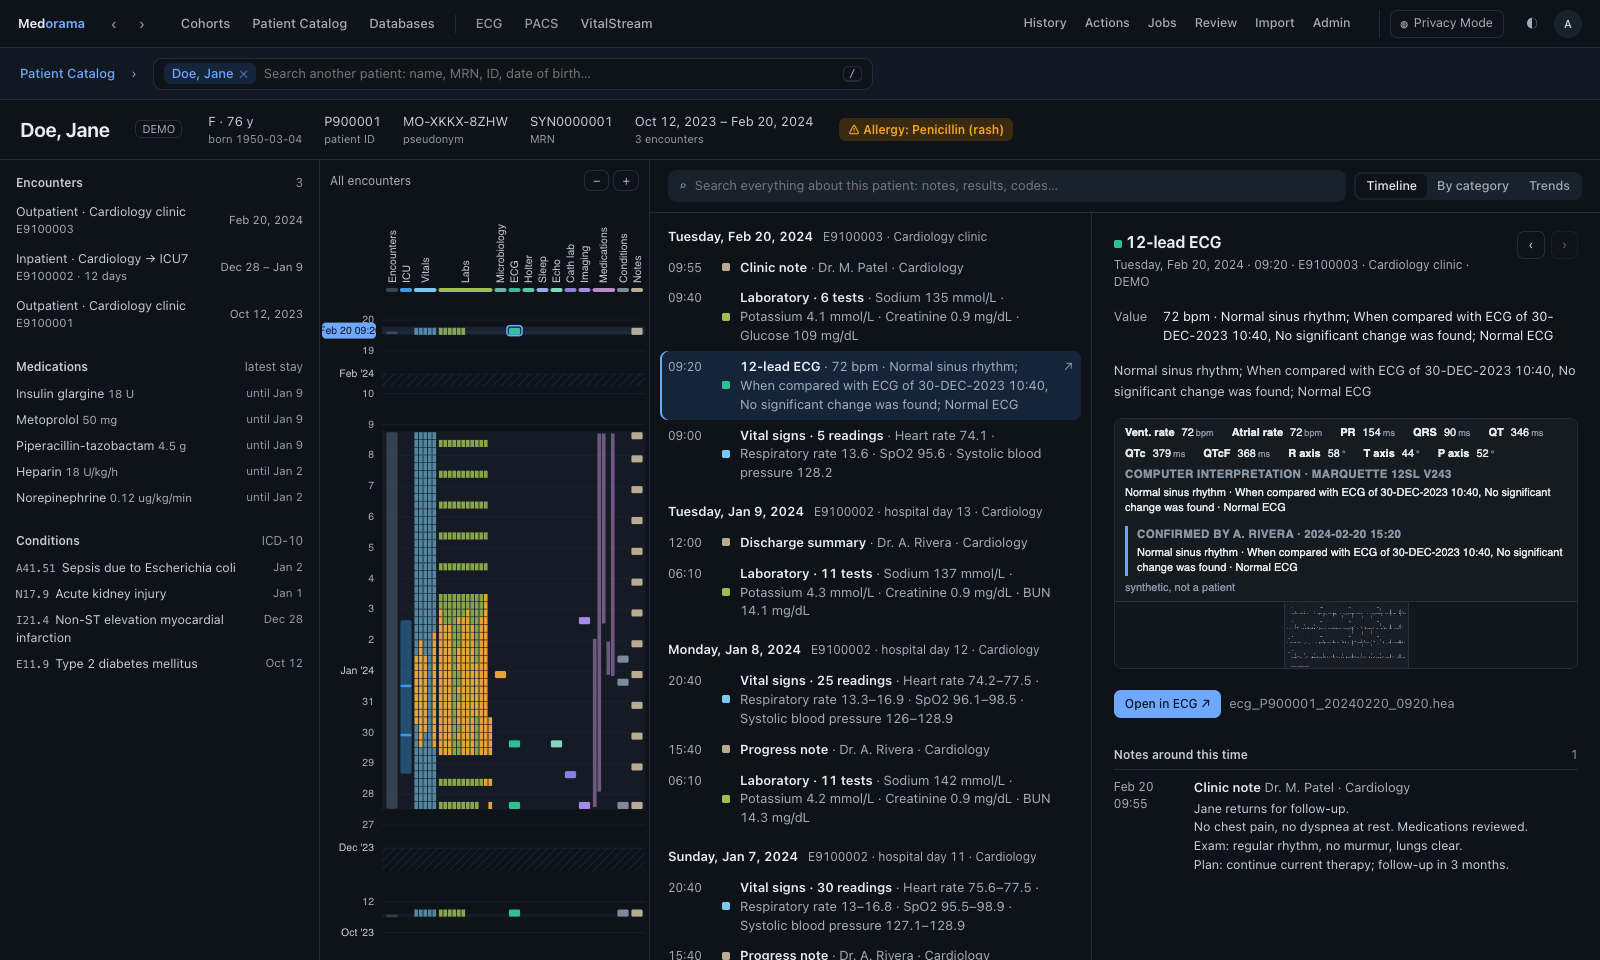
\includegraphics[width=\linewidth]{patient.png}
\end{minipage}\hfill
\begin{minipage}[t]{0.49\linewidth}\centering
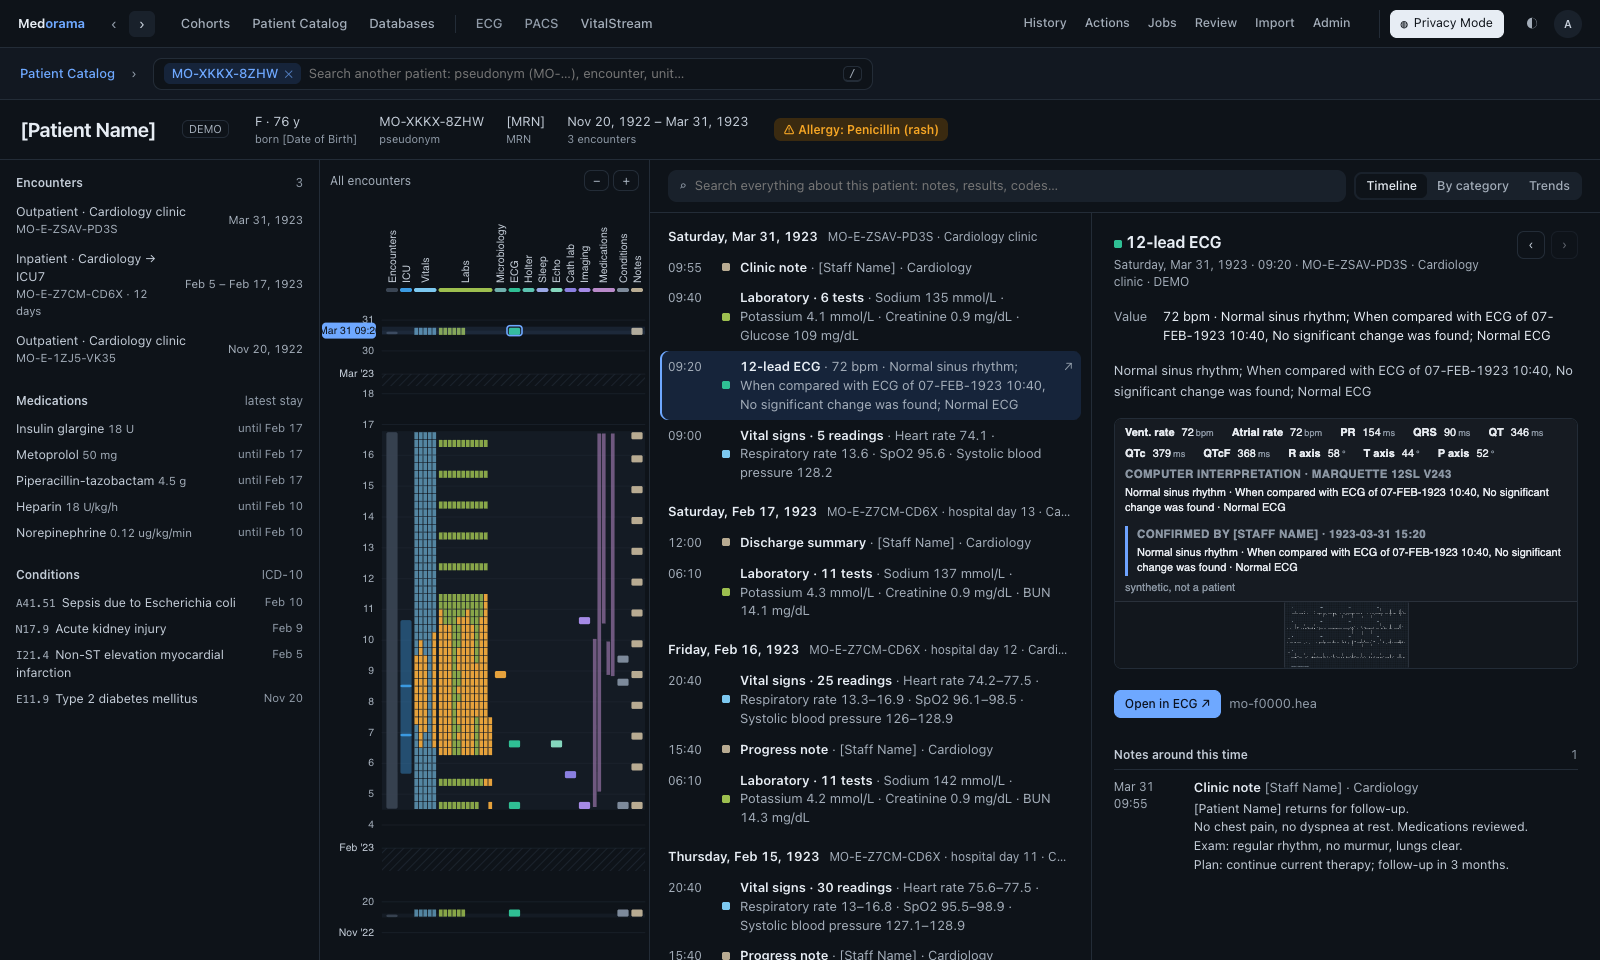
\includegraphics[width=\linewidth]{privacy.png}
\end{minipage}
\caption{The same synthetic patient, identified (left) and in Privacy Mode
(right).}\label{fig:protecting-compare}
\end{figure}

\section{Terms used in this chapter}
\label{sec:protecting-terms}

\begin{xltabular}{\linewidth}{@{}P{3.2cm}L@{}}
\caption{The terms of patient-data protection.}
\label{tab:protecting-terms}\\
\toprule
\tabhead Term & \tabhead Meaning \\
\midrule
\endfirsthead
\toprule
\tabhead Term & \tabhead Meaning \\
\midrule
\endhead
\bottomrule
\endfoot
PHI & Protected health information: anything that can identify a patient, together with their
  health data. \\
Catalog & Medorama's own database of patients, encounters, clinical entries, recordings, users
  and the audit log (SQLite or PostgreSQL). \\
Identifier & A value that names a person directly: a name, a medical record number (MRN), a date
  of birth, an account number (CSN), an imported patient or encounter ID. \\
PHI permission & A right that an administrator gives to a user account. Without it, a user can
  never see identifiers. \\
Privacy Mode & The state of a session in which every answer passes the privacy gate. \\
Privacy gate & The server code that de-identifies answers and files for sessions in Privacy
  Mode, and refuses what it cannot de-identify. \\
Pseudonym & A random code that stands for a patient (\code{MO-XXXX-XXXX}) or an encounter
  (\code{MO-E-XXXX-XXXX}) in Privacy Mode. \\
Placeholder & Fixed text that stands for a withheld value, such as \code{[Patient Name]} or
  \code{[MRN]}. \\
Date offset & The amount by which Privacy Mode moves a patient's dates back: the catalog's
  offset plus the patient's own number of days. \\
Connected database & A database that Medorama reads in place, such as an OMOP instance, instead
  of importing it. \\
\end{xltabular}

\section{Privacy Mode and the PHI permission}
\label{sec:protecting-modes}

Every session is in Privacy Mode unless its user has the PHI permission and has switched Privacy
Mode off. \Cref{tab:protecting-who} gives the defaults.

\begin{xltabular}{\linewidth}{@{}P{6.6cm}L@{}}
\caption{Who is in Privacy Mode.}
\label{tab:protecting-who}\\
\toprule
\tabhead User & \tabhead Privacy Mode \\
\midrule
\endfirsthead
\toprule
\tabhead User & \tabhead Privacy Mode \\
\midrule
\endhead
\bottomrule
\endfoot
Without the PHI permission (any role) & Always on. It cannot be switched off. \\
With the PHI permission, not an administrator & On when the user signs in. The user may switch
  it off. \\
Administrator with the PHI permission & Off when the user signs in. The administrator may switch
  it on. \\
\end{xltabular}

The role of a user (viewer, analyst or administrator) decides what the user may \emph{do}; the
PHI permission decides what the user may \emph{see}. An administrator grants the PHI permission
when creating an account, or later in \ui{Admin} $\rightarrow$ \ui{Users}
(\cref{chap:users-privacy}). Most users should not have it: they work with pseudonyms and shifted
dates, which is enough for most research.

\paragraph{Switching Privacy Mode.} The \ui{Privacy Mode} switch in the page's header changes the
mode for that session. The server keeps the choice with the session, never in the browser, and
writes an entry to the audit log (\code{privacy\_on} or \code{privacy\_off}): leaving Privacy
Mode is always audited. The page then reloads, so that nothing identified stays on the screen
after Privacy Mode is switched on. A user without the PHI permission who asks to leave Privacy
Mode is refused (HTTP 403). Every sign-in starts in the user's default mode, so whoever uses the
browser next starts there too. Signing out, or a session that ends while the page is open,
reloads the page: the next person to sign in at that browser sees nothing of what the previous
user saw.

A session in Privacy Mode is treated exactly like a user without the PHI permission: the server
replaces the session's user with a copy that has no PHI permission (\file{users.rs},
\code{User::in\_privacy\_mode}), so every check that depends on the permission fails closed for
that session.

\paragraph{For reviewers.} The decision is \file{server.rs} \code{in\_privacy} and
\code{session\_user}; the switch is \file{server.rs} \code{set\_privacy}. It is tested in
\file{medorama/tests/privacy.rs}: a user without the permission is refused, and an administrator
who switches Privacy Mode on receives no identifier.

\section{What is withheld and what replaces it}
\label{sec:protecting-withheld}

\subsection{Identifiers and dates}
\label{sec:protecting-identifiers}

\Cref{tab:protecting-replaced} lists what Privacy Mode withholds by default and what the user sees
instead. The defaults follow the identifiers of the HIPAA Safe Harbor list that the catalog
holds, with one exception, the text of notes, described in \cref{sec:protecting-notes}.

\begin{xltabular}{\linewidth}{@{}P{5.0cm}L@{}}
\caption{What Privacy Mode withholds, and what replaces it.}
\label{tab:protecting-replaced}\\
\toprule
\tabhead Data & \tabhead In Privacy Mode \\
\midrule
\endfirsthead
\toprule
\tabhead Data & \tabhead In Privacy Mode \\
\midrule
\endhead
\bottomrule
\endfoot
Patients' names & \code{[Patient Name]} \\
Staff names (authors of notes, ECG overreaders, physicians) & \code{[Staff Name]} \\
Medical record numbers & \code{[MRN]} \\
Account numbers (CSN) & \code{[CSN]} \\
Dates of birth & \code{[Date of Birth]}. The age is computed on the server and shown instead. \\
Imported patient IDs & The patient's pseudonym, \code{MO-XXXX-XXXX}, because an imported ID may
  be an MRN. In a database's own columns, \code{[Patient ID]}. \\
Imported encounter IDs & The encounter's pseudonym, \code{MO-E-XXXX-XXXX}. \\
Every date and time & Moved back by the patient's date offset (\cref{sec:protecting-dates}). \\
Ages above 89 & \code{90+} \\
Recordings' paths and file names & Tokens (\code{mo-rec:<n>}, \code{mo-f0003.dcm}), and
  \code{[Recording]} or \code{[File Name]} where a name is shown. \\
An identifier found inside text & The same replacement wherever it appears (MRNs, account
  numbers, and imported IDs of four or more characters that contain a digit). \\
Columns of imported databases that hold identifiers & Kept under their imported names. Their
  cells become placeholders, so the table keeps the shape of the source. \\
Columns that the catalog does not recognize & Withheld (\code{[Withheld]}), except measurement
  columns such as \code{QT (ms)}, which hold numbers. In the \ui{Databases} tab, the search, the
  filters and the sorting skip such columns. \\
The text of notes and reports & Shown by default, with the patient's own names and date of birth
  replaced, and marked with a warning. Withheld (\code{[Withheld]}) when the administrator
  chooses so (\cref{sec:protecting-notes}). \\
\end{xltabular}

Placeholders are fixed text. They never reveal the length or the form of the value they replace.

\subsection{Pseudonyms}
\label{sec:protecting-pseudonyms}

Each patient receives a pseudonym such as \code{MO-D5QM-Y1X5} when first seen, and each encounter
one such as \code{MO-E-QMC6-E2VA}. In Privacy Mode, users find patients by these pseudonyms, and
exports name patients by them.
\begin{itemize}
\item \textbf{Random and stored, never derived.} The seven characters come from the operating
  system's secure random generator, and an eighth is a check character. No calculation on an MRN
  or a name produces the pseudonym: the only link between a pseudonym and a person is the catalog
  database. This follows HIPAA 45 CFR \S164.514(c), which asks that a re-identification code not
  be ``derived from or related to information about the individual'', and ISO/TS 25237.
\item \textbf{Why not a hash of the MRN.} MRNs are short, so every possible MRN can be hashed in
  minutes, which would reverse an unkeyed hash. A keyed hash would depend on one secret forever
  and would still be derived from the identifier.
\item \textbf{Stable.} A patient keeps the same pseudonym through re-imports and restarts. When
  two records are merged as one person, the absorbed record's pseudonym stays as an alias, so
  that earlier exports and cohort definitions still resolve.
\item \textbf{Checked.} The check character (Luhn mod 32, in Crockford's base 32, which has no I,
  L, O or U) catches any single mistyped character, so a pseudonym typed into a search is either
  right or refused.
\item \textbf{The same everywhere.} Pages, exports, cohort definitions and their history, DICOM
  headers and plug-ins' job descriptions use the same pseudonym.
\end{itemize}
A catalog rebuilt from scratch draws new pseudonyms and new date offsets. Keep backups of the
database to keep them stable (\cref{sec:deployment-backups}).

\subsection{Dates and ages}
\label{sec:protecting-dates}

Research depends on the time between events, so Privacy Mode moves dates rather than removing
them.
\begin{itemize}
\item \textbf{The catalog's offset.} Every date and time moves back by an offset that the
  administrator sets in years, months, days and hours (\ui{Admin} $\rightarrow$ \ui{Privacy
  Mode}). It is counted on the calendar from 2000-01-01. The default is 36\,570 days, about 100
  years.
\item \textbf{Each patient's own days.} On top of that, each patient's dates move back by a whole
  number of days between 0 and a maximum (\code{spread\_days}: 365 by default, at least 30 and
  at most 3650; a smaller value saved before that minimum is kept, since raising it moves every
  patient's dates, and \cmd{medorama serve} warns about it at start). This number is drawn at
  random once, when the patient's
  pseudonym is drawn, and stored with it. Every user and every session therefore sees the same
  dates for the same patient. Something that names no patient moves by the catalog's offset
  alone.
\item \textbf{Intervals are kept.} The time between any two events of one patient is exact.
  Between two patients, it changes by the difference of their own days.
\item \textbf{Row by row.} A patient's pages and files move by that patient's offset; a list or an
  export moves row by row, by the patient each row names; a recording in VitalStream moves by the
  patient of its encounter.
\item \textbf{Everywhere.} Dates move in every form the catalog holds or sends: numbers (Unix
  times), text (\code{2024-01-02} with or without a time, \code{2024/01/02}, \code{01/02/2024},
  \code{2.1.2024}, \code{02-JAN-2024}, \code{Jan 2, 2024}, \code{2 January 2024},
  \code{20240102}), BedMaster file names' Unix times (a name whose moved time falls before 1970
  is written with a minus sign: \code{ICU7\_12--1455465600}), DICOM dates and times, GE MUSE XML
  dates, WFDB base dates, EDF start dates, and the keys of entries that carry a time
  (\code{labs:<encounter>:<time>}). A date written \code{01/02/2024} is read month first, unless
  the catalog writes dates day first (\ui{Admin} $\rightarrow$ \ui{Dates and times}) or the
  month would be over 12; \code{2.1.2024} is read day first. Either way the year moves back by
  about a century, so a misread date shows no real date. A Unix time written on its own is a
  number, and is kept.
\item \textbf{Searches and criteria in Privacy Mode.} A search, a filter or a sort uses only what
  the session is shown (pseudonyms, file tokens, each patient's dates as shown), so it cannot test
  a real value. A date a user types, in a cohort criterion or a date filter, is a date as shown:
  the server compares it with each patient's dates as that session sees them, so the criterion
  means exactly what the page says. The page never holds the date offset: only administrators
  may read it (\code{GET deid}).
\item \textbf{Ages} are computed on the server from the date of birth, which never leaves it.
  Ages above 89 are shown as \code{90+}.
\end{itemize}

\begin{note}
Date shifting is pseudonymization, not anonymization. Anyone who learns the real date of one of a
patient's events can re-date all of that patient's events, and every other patient's to within
\code{spread\_days}. Record the offset under your governance, and keep it confidential.
\end{note}

\subsection{Text and notes}
\label{sec:protecting-notes}

Free text, such as clinical notes and reports, can name the patient, relatives or staff in ways
that no rule can recognize reliably. By default, Privacy Mode shows the text of notes, because it
is often essential for research, with the following protections:
\begin{itemize}
\item the patient's own names (each word of at least two letters, and each part of a compound
  name such as \code{Smith-Jones} or \code{O'Brien}) and date of birth are replaced by
  \code{[Patient Name]} and \code{[Date of Birth]};
\item identifiers the catalog knows (MRNs, account numbers, imported IDs of four or more
  characters that contain a digit) are replaced wherever they appear, and so are recordings'
  paths and the folders they lie in (\code{[Folder]}), which may be named after the patient;
\item phrases such as ``Confirmed by \dots'' or ``Signed by \dots'' are replaced by
  \code{[Staff Name]};
\item dates in the text are moved back;
\item the page marks the text with a warning, because it may still identify someone.
\end{itemize}
An administrator who prefers to withhold all free text ticks \ui{The text of notes and reports}
in \ui{Admin} $\rightarrow$ \ui{Privacy Mode}. Notes then appear as \code{[Withheld]}, and their
text is not searched in Privacy Mode. The same choice applies to the annotations of EDF+
recordings shown in VitalStream (\cref{sec:protecting-vitalstream}).

\subsection{Searches}
\label{sec:protecting-searches}

In Privacy Mode, a search by name, MRN, date of birth, account number or a withheld column is
refused with a message (HTTP 400). A plain word does not match identifiers behind the scenes
either: otherwise the number of results would reveal whether a person is in the catalog.
Patients are found by their pseudonyms, and encounters by theirs. Every search, filter and sort
uses only what the session is shown: pseudonyms, tokens and placeholders, and each patient's
dates as they are shown, so a search for a real identifier or a real date finds nothing, and
lists are ordered by the dates shown. Searches of identifiers by users who may see them are
written to the audit log (\code{phi\_search}), and so are searches, filters and cohort criteria
made in Privacy Mode, with their text (\code{privacy\_search}).

\subsection{What the administrator can change}
\label{sec:protecting-settings}

\ui{Admin} $\rightarrow$ \ui{Privacy Mode} lets an administrator choose which kinds of identifiers
are withheld, the catalog's offset and \code{spread\_days} (\cref{sec:users-privacy-settings}).
Every change is written to the audit log (\code{deid\_settings}) with the new settings. Some
protections do not depend on these settings and always apply in Privacy Mode: imported patient
and encounter IDs become pseudonyms, file names become tokens, staff names become
\code{[Staff Name]}, unrecognized columns are withheld, and files that the gate cannot
de-identify are refused.

\paragraph{For reviewers.} Placeholders, the identifier dictionary and table cells are in
\file{gate.rs} (\code{Dict}, \code{Restricted::json}, \code{column\_placeholder},
\code{column\_mask}); dates, ages and the settings in \file{deid.rs} (\code{FIELDS},
\code{Settings}, \code{answer\_with}, \code{shift\_text}); pseudonyms in \file{pseudonyms.rs}.
Each module has unit tests, and \file{medorama/tests/privacy.rs} tests them end to end.

\section{De-identifying files at the source}
\label{sec:protecting-files}

Patients' files (ECGs, recordings, DICOM studies, documents) are sent one item at a time, through
\code{patients/\{id\}/file/\{item\}}, and only the files that belong to that item. In Privacy
Mode, the gate decides how each file leaves according to its kind
(\cref{tab:protecting-files}). A file is de-identified as it is sent; the original on disk is
never changed.

\begin{xltabular}{\linewidth}{@{}P{3.6cm}L@{}}
\caption{How each kind of file leaves in Privacy Mode.}
\label{tab:protecting-files}\\
\toprule
\tabhead Kind of file & \tabhead In Privacy Mode \\
\midrule
\endfirsthead
\toprule
\tabhead Kind of file & \tabhead In Privacy Mode \\
\midrule
\endhead
\bottomrule
\endfoot
WFDB header (\file{.hea}) & Comments that identify the patient (name, ID, MRN, date of birth,
  address, phone, however their key is written: \code{Patient\_Name:}, \code{Name=},
  \code{Patient name -}, \code{Birthdate:}) are removed; the patient's own names and date of
  birth are replaced in every other comment; staff named in comments become
  \code{[Staff Name]}; the base date and dates in comments are moved back; ages above 89 become
  \code{90+}; the record's name and its signal files' names are replaced by tokens. \\
WFDB samples (\file{.dat}) & Sent as they are (they hold only numbers) when a header of the same
  item names them; any other \file{.dat} file is refused. \\
GE MUSE XML (\file{.xml} with a \code{RestingECG} element) & The patient's demographics are
  removed except age (capped) and sex, whatever attributes or spaces their tags hold; the order
  is removed; staff names become \code{[Staff Name]} and their IDs are emptied; a patient's name
  elsewhere becomes \code{[Patient Name]}; the patient's own names and date of birth are replaced
  in the statements; ``Confirmed by'' phrases are replaced; every date is moved back. A file that
  still holds a patient's name, ID or date of birth after all this is refused, as is any other
  XML file. \\
DICOM (\file{.dcm}, \file{.dicom}, or a file recognized by its content) & The header is
  rewritten with the actions of the DICOM confidentiality profile for the attributes listed
  (\cref{sec:protecting-dicom}); the pixel data are copied byte for byte. The file is marked as
  possibly identifying. \\
EDF, EDF+, BDF, BDF+ (\file{.edf}, \file{.bdf}) & The header is de-identified and the texts of
  annotations are removed; the samples are sent as they are (\cref{sec:protecting-edf}). \\
Pictures, videos and PDF documents & Sent as they are, marked as possibly identifying: the
  viewer's tab shows an amber warning triangle. \\
Anything else & Refused (HTTP 403). \\
\end{xltabular}

\paragraph{File names never leave.} In Privacy Mode, an item's files are named by tokens
(\code{mo-f0000.hea}, \code{mo-f0001.dat}), and a request that gives a real file name is not
accepted. Answers that carry files vary with the session cookie (\code{Vary: Cookie}), so a
browser never shows a cached identified copy in Privacy Mode.

\subsection{DICOM}
\label{sec:protecting-dicom}

The rewrite applies the actions of DICOM PS3.15 Table E.1-1, the \textbf{Basic Application
Level Confidentiality Profile} (\code{X}: removed; \code{Z}: emptied; \code{D}: a dummy value;
\code{U}: a new UID), for the attributes listed in \file{dicom.rs} (\code{PROFILE}), with the
\textbf{Retain Longitudinal Temporal Information with Modified Dates} option: dates are moved by
the patient's date offset, instead of removed (\cref{tab:protecting-dicom}). It is not a
certified implementation of the profile: an attribute of the table that the list lacks is kept,
with its free text scrubbed as below. The De-identification Method written into the file says
so.

\begin{xltabular}{\linewidth}{@{}P{5.6cm}L@{}}
\caption{DICOM elements in Privacy Mode.}
\label{tab:protecting-dicom}\\
\toprule
\tabhead Element & \tabhead In Privacy Mode \\
\midrule
\endfirsthead
\toprule
\tabhead Element & \tabhead In Privacy Mode \\
\midrule
\endhead
\bottomrule
\endfoot
Patient's Name & \code{[Patient Name]} \\
Patient ID & The patient's pseudonym \\
Patient's Birth Date & Emptied \\
Patient's Age & Capped at 90 years when ages are capped \\
Patient's Sex, Size and Weight & Kept \\
Every other element of the patient group (0010) & Removed \\
The clinical trial module (0012) & Removed \\
Other person names (referring, performing and reading physicians, operators, observers) &
  \code{[Staff Name]} \\
The attributes of the list: institution, department, station, addresses and phones, device,
  detector and other equipment IDs, accession, study, order, procedure, admission and visit IDs;
  descriptions (study, series, requested and performed procedures, derivation, admitting and
  discharge diagnoses); comments (image, study, acquisition, identifying, performed procedure
  step, visit); protocol names; structured report text and content (Text Value, Content
  Sequence); graphic annotations; icon images; digital signatures & Removed (\code{X}), or
  emptied (\code{Z}: accession, institution name, study ID, order numbers) \\
Curves (50xx), overlays (60xx: their bitmaps, labels and comments), the retired results group
  (4008) & Removed \\
Free text left (SH, LO, ST, LT, UC, UT; in implicit-VR files, elements of unknown VR that hold
  text) & The patient's own names and date of birth, and the identifiers the catalog knows,
  replaced; dates in it moved back \\
Private elements & Removed \\
Instance UIDs (study, series, instance, frame of reference, references) & Replaced by
  \code{2.25.} and 128 bits of an HMAC-SHA-256 under the catalog's secret, so that a series still
  holds together and nobody without the secret can map them back. The standard's own UIDs
  (classes, transfer syntaxes) are kept. \\
Dates and times & Moved back, a date and its time together \\
Patient Identity Removed, De-identification Method, Longitudinal Temporal Information Modified &
  Added (\code{YES}, the method, \code{MODIFIED}) \\
\end{xltabular}

The file keeps its transfer syntax (explicit or implicit VR little endian, and every compressed
syntax). In implicit VR the file does not say which elements are person names: the rewrite knows
the person names of the standard's dictionary by their tags. Deflated and big-endian files are
refused, because they could not be rewritten safely, and so are files with sequences nested more
than 32 deep.
Real files from several vendors and syntaxes (CT in implicit and explicit VR, JPEG Lossless, JPEG
Extended 12-bit, multi-frame JPEG Baseline angiography, panoramic X-ray) were checked with pydicom
after the rewrite: no original identifier and no private element remained, and the pixels were
identical (\file{medorama/tests/dicom\_samples.rs}).

What the pixels show is not changed. Ultrasound images, secondary captures and scanned documents
may carry names burned into the image, so every DICOM file is sent with the ``may contain PHI''
mark.

\subsection{EDF and BDF}
\label{sec:protecting-edf}

An EDF or BDF header has two identification fields of 80 characters, one for the patient and one
for the recording, and states the recording's start date and time
(\cref{sec:recordings-edf}). In Privacy Mode, a file sent to the browser is rewritten as follows
(\file{deid.rs} \code{edf\_header} and \code{edf\_annotations}, called by \file{server.rs}
\code{edf\_deidentified}):
\begin{itemize}
\item the patient field becomes \code{X X X X}, EDF+'s form for an anonymous patient;
\item in EDF+ and BDF+ files, the recording field becomes \code{Startdate dd-MMM-yyyy X X X},
  with the start date moved back; in plain EDF and BDF files, whose recording field is free
  text, it is left blank;
\item the start date and time are moved back. EDF writes two-digit years for 1985 to 2084 only:
  an EDF+ file whose moved date falls outside that range has \code{yy} in its date field and the
  full year in its recording field, as EDF+ prescribes, and a plain EDF file states no start date
  rather than a wrong one;
\item in EDF+ and BDF+ files, the texts of annotations are removed. Each data record keeps only
  its time-keeping annotation (its onset), so that the file's timing stays whole; the bytes after
  the last whole data record are left out;
\item the samples are sent as they are.
\end{itemize}
A file without annotation signals is streamed, and only its header is rewritten. A file with
annotation signals is rewritten whole in memory, so EDF+ files with annotations larger than 64\,MB
are refused in Privacy Mode; such recordings can still be opened in VitalStream. The technical
fields of the signal headers (labels, units, transducer and prefiltering descriptions) are kept
as they are.

The engine and the viewers never put the patient and recording fields into an index or into any
answer. Medorama's \code{identify} action reads them into the catalog's identifier tables, where
an administrator can check that the file belongs to the patient it is linked to
(\cref{chap:administration}).

\subsection{Why some files pass with a warning}
\label{sec:protecting-warning}

Pictures, videos, PDF documents and DICOM pixels are images: the gate cannot read what they show,
and removing burned-in text would require optical character recognition, which Medorama does not
do. Refusing them would make imaging research impossible in Privacy Mode, so they are sent as they
are, with the header \code{x-medorama-may-contain-phi}, and the page shows an amber warning
triangle on the tab that displays them. Every other kind of file that the gate cannot de-identify
is refused.

\paragraph{For reviewers.} The file rules are \file{gate.rs} \code{FileKind} and
\code{file\_kind}, and \file{server.rs} \code{attachment\_response}. WFDB headers are
\file{deid.rs} \code{wfdb\_header}; MUSE XML is \file{deid.rs} \code{muse\_xml}; DICOM is
\file{dicom.rs}; EDF is \file{deid.rs} \code{edf\_header} and \code{edf\_annotations}, called by
\file{server.rs} \code{edf\_deidentified}. File tokens are \file{gate.rs} \code{file\_token} and
\code{token\_index}.

\section{The VitalStream viewer}
\label{sec:protecting-vitalstream}

The VitalStream waveform viewer runs as a separate program on the server, reachable only through
Medorama's \emph{gateway} (\file{/viewer/}; \cref{sec:architecture-gateway}). The viewer itself
never reads names or dates of birth from any recording. In Privacy Mode, the gateway adds the
following rules:
\begin{itemize}
\item recordings are opened by token (\code{mo-rec:<n>}), never by path, and a path sent by the
  page is refused;
\item browsing and scanning folders is refused, because folder and file names may identify;
\item the times that the page sends are moved forward before they reach the viewer, and every
  time in the viewer's answers is moved back, by the recording's patient's date offset;
\item a dataset's path and name are replaced by its token and \code{[Recording]};
\item the annotations of EDF+ and BDF+ recordings, which are free text and are shown as events in
  VitalStream's Annotations lane, are treated like notes: when Privacy Mode withholds the text of
  notes, each annotation reads \code{[Annotation]}; otherwise the patient's own names and date of
  birth are replaced (\file{gateway.rs}, \code{gate\_annotations});
\item every answer then passes the gate's last layer, like any other answer, which replaces the
  identifiers the catalog knows and moves dates back.
\end{itemize}

\paragraph{For reviewers.} \file{gateway.rs} (\code{handle}, \code{shift\_query},
\code{gate\_annotations}, with its unit test \code{annotations\_in\_privacy\_mode}); tested with a
real viewer in \file{medorama/tests/gateway.rs}.

\section{Exports and plug-in actions}
\label{sec:protecting-exports}

\begin{itemize}
\item \textbf{Exports} made in Privacy Mode (cohort members, definitions, members' data, Excel
  files, database CSV files) pass the same gate. They have the same columns as identified
  exports, with identifiers as placeholders, patients named by pseudonym and dates moved back,
  and their file names end in \code{-privacy}. Exports by users who see identifiers are written
  to the audit log (\code{phi\_export}).
\item \textbf{Plug-in actions}, programs that an administrator installs to analyze recordings,
  receive a job description with the recording's path, its index folder, an output folder, and
  the pseudonyms of its encounters and patients, never their imported IDs (\cref{chap:actions}).
  They also do not receive the server's secrets in their environment
  (\cref{sec:security-jobs}).
\end{itemize}

\section{Connected databases}
\label{sec:protecting-connected}

A connected database (an OMOP instance, a data warehouse read through SQL views) is read in
place, read-only, and its data leave through the same gate as the catalog's.
\begin{itemize}
\item \textbf{Only canonical columns are read.} Medorama reads a connected database through three
  views of fixed columns (persons, visits, entries), each column with a privacy class: key,
  identifier, date, free text, staff or clinical value. A view cannot add a field that the gate
  does not know (\cref{chap:connecting}).
\item \textbf{Persons are linked to patients.} A connected database's persons are linked to the
  catalog's patients, so they leave as pseudonyms. Their identifiers are copied into the
  catalog's identifier tables, where the gate knows them, and their keys in the source database
  never leave.
\item \textbf{Entries are named by tokens.} An entry is named by a keyed hash
  (\code{live:<connection>:<token>}) that holds neither its key nor its time. Its dates move back
  with the rest, its text follows the rule for notes, and its authors are treated as staff.
\item \textbf{Searches} of identifiers in connected databases need the PHI permission, as in the
  catalog.
\end{itemize}

\paragraph{For reviewers.} \file{sources/} (read-only sessions, views, the person registry in
\file{sources/link.rs}) and \file{patient/items.rs} \code{live\_items}; tested in
\file{medorama/tests/connections.rs} over a synthetic OMOP database, in SQLite and PostgreSQL.

\section{Failing closed}
\label{sec:protecting-fail-closed}

Most answers are de-identified by the code that builds them, because that code knows what each
value is. A last layer of the server then enforces the rule for every answer of a session in
Privacy Mode:
\begin{itemize}
\item a JSON answer passes through the gate there, whatever the endpoint;
\item a file passes only if the gate cleared it;
\item any other answer that carries data is refused (HTTP 403), and the refusal is written to the
  server's error output.
\end{itemize}
The pages and scripts of the web interface, redirects and error messages hold no patient data and
pass unchanged. As a result, a new endpoint whose author forgets the gate cannot leak identifiers:
its answer is either refused or de-identified. This is why the gate is said to \emph{fail
closed}. In the same spirit, a session in Privacy Mode is handled as a user without the PHI
permission, so a forgotten permission check also errs on the side of withholding.

\paragraph{For reviewers.} \file{server.rs} \code{privacy} (the last layer), and \code{cleared}
and \code{may\_hold\_phi} (the marks set by handlers). The internal header
\code{x-medorama-gate} is removed before an answer leaves.

\section{How the design is verified}
\label{sec:protecting-verified}

\begin{itemize}
\item \textbf{End to end.} \file{medorama/tests/privacy.rs} seeds a catalog with identifiers that
  cannot appear by chance: a name, an MRN, patient, encounter and account numbers, a date of
  birth, staff names, an institution, and real dates in the forms that tables, DICOM, MUSE, WFDB,
  EDF and EDF+ write them. They are placed in every format the catalog serves: tables, notes, a
  WFDB record, GE MUSE XML, DICOM, an EDF+ file, a picture, a text file and an ICU recording. The
  test then requests every page's answers, every entry's detail, every file and its parts, and
  every cohort and database export, as a user without the PHI permission and as an administrator
  who switched Privacy Mode on. It asserts that no byte of any answer holds any of the seeded
  identifiers, that no JSON number is a real time, that identifier searches are refused or find
  nobody, that placeholders and pseudonyms appear, that the text file is refused, and that
  pictures and DICOM files are marked. It also checks that the identified answers do hold the
  identifiers, so that the test would fail if it checked nothing.
\item \textbf{The viewer.} \file{medorama/tests/gateway.rs} runs a real VitalStream viewer behind
  the gateway, in Privacy Mode too.
\item \textbf{Connected databases.} \file{medorama/tests/connections.rs} repeats the Privacy Mode
  check over a synthetic OMOP database.
\item \textbf{Each de-identifier.} Unit tests in \file{gate.rs}, \file{deid.rs} (including real
  EDF test files), \file{dicom.rs}, \file{pseudonyms.rs} and \file{gateway.rs};
  \file{medorama/tests/dicom\_samples.rs} checks real DICOM files with pydicom.
\end{itemize}
The commands that run these tests are listed in \cref{sec:security-verifying}.

\section{What Privacy Mode cannot do}
\label{sec:protecting-limits}

Privacy Mode reduces what users see; it does not make data anonymous. Reviewers and users should
know its limits.
\begin{itemize}
\item \textbf{Burned-in text.} Names written into pictures, scanned PDFs, video frames and DICOM
  pixels are not removed. These files are marked with the amber warning instead.
\item \textbf{Free text.} Notes, reports and EDF+ annotations may name the patient, relatives or
  staff in ways that no rule recognizes. They are marked where they are shown, and an
  administrator can withhold them entirely.
\item \textbf{Quasi-identifiers.} Sex, a capped age, rare diagnoses, units and beds, small cohorts
  and exact intervals can single out a person when combined with outside knowledge.
\item \textbf{Date offsets.} Learning one real date of a patient reveals that patient's offset,
  and every other patient's to within \code{spread\_days}.
\item \textbf{Not Safe Harbor.} Because dates are shifted rather than removed, data viewed or
  exported in Privacy Mode are not de-identified under HIPAA's Safe Harbor method. They suit use
  as a limited data set under a data use agreement, or under an expert determination
  (\cref{sec:security-regulatory}).
\item \textbf{Everyone sees every patient.} Medorama has no per-patient or per-study access
  lists: every signed-in user may see every patient of a catalog, as Privacy Mode and the PHI
  permission allow. Separate catalogs serve separate studies.
\end{itemize}

\begin{phibox}
The deploying institution remains responsible for the rest: who receives accounts and the PHI
permission, how the server and its backups are protected, which data are imported, and how
exports are used and shared. The deployment checklist (\cref{sec:security-checklist}) lists these
duties. Treat what a session in Privacy Mode exports as pseudonymized data, not as anonymous
data.
\end{phibox}

\section{The repository holds no patient data}
\label{sec:protecting-repository}

Medorama's source repository contains no patient data. Tests and demonstrations use synthetic
data only, or public data sets kept outside the repository. A privacy check
(\file{tools/git-hooks/check-files}), run by the pre-commit and pre-merge-commit hooks on what
git would store, refuses recordings, data files, DICOM and MUSE XML files (recognized by their
content), notebooks with outputs, real recording names and anything in a \file{sample\_data/}
folder. CI runs the same check on every commit of each pull request and push, and on every file
(\file{.github/workflows/checks.yml}), so a commit made without the hooks is still caught before
it is merged. The rules are in the repository's \file{PRIVACY.md}.

% The security and privacy review, docs/security.md in full: executive summary, scope, trust
% boundaries, assets, threat model, authentication, authorization, Privacy Mode and the gate
% (controls, file rules, fail closed, pseudonyms, verification), data at rest and in transit,
% web application security, untrusted input, audit logging, background jobs and plug-ins, supply
% chain, regulatory mapping, the deployment checklist, limitations, verification.
% The code is the authority (medorama/src/server.rs, signin.rs, users.rs, gate.rs, deid.rs,
% dicom.rs, pseudonyms.rs, gateway.rs, audit.rs, actions.rs, db.rs, sql/pg.rs, config.rs).
\chapter{Security and privacy review}
\label{chap:security}

This chapter is for the people who decide whether Medorama may run on their institution's
patient data: IT security reviewers, privacy officers, and IT and research administrators. It
describes what Medorama protects, against whom, how, and what it leaves to the deploying
institution. Each control names the code that implements it and the test that checks it, so that
every claim can be verified rather than taken on trust. It follows the repository's
\file{docs/security.md}.

The chapter describes Medorama \mdversion{} (unreleased). Medorama is research software, not a
medical device, and it holds no certification. To report a vulnerability, follow the
repository's \file{SECURITY.md}. The system's parts are described in \cref{chap:architecture}, a
plain-language explanation of how identifiers are hidden is \cref{chap:protecting}, and sign-in
is described in \cref{chap:sign-in}.

\section{Executive summary}
\label{sec:security-summary}

Medorama is a single server program, written in Rust, that an institution runs on its own hosts.
It serves a web page and three viewers to the institution's users, and reads patient data from
imported tables, files and connected databases. It sends nothing to any third party: no
telemetry, no external services, and no scripts or fonts from other sites.
\begin{itemize}
\item \textbf{One way in.} Every request passes Medorama's sign-in. Users sign in either with
  Medorama's own accounts (Argon2id password hashes, throttling, hashed session tokens) or
  through the institution's authenticating reverse proxy, which brings single sign-on and
  multi-factor authentication. The sign-in method is one module (\file{signin.rs}); roles and
  permissions are decided in Medorama, on the server, for every request.
\item \textbf{Identifiers in one place.} Names, medical record numbers, dates of birth, account
  numbers and imported IDs are kept only in the catalog database, in their own tables. The
  viewers, indexes, results and plug-ins receive pseudonyms only.
\item \textbf{Privacy Mode by default.} Users without the PHI permission are always in Privacy
  Mode, and users with it start in Privacy Mode unless they are administrators. In Privacy Mode,
  the privacy gate de-identifies every answer as it is sent: identifiers become placeholders and
  random pseudonyms, dates move back by a per-patient offset, and files are de-identified at the
  source (WFDB, GE MUSE XML, DICOM with the actions of PS3.15's Basic Profile for the
  attributes it lists, EDF and BDF). Pictures,
  videos and PDF documents pass with a warning; any other file is refused.
\item \textbf{Fail closed.} A last layer of the server puts every JSON answer of a Privacy Mode
  session through the gate and refuses any other answer that the gate did not clear, so a new
  endpoint that forgets the gate cannot leak identifiers. An end-to-end test seeds identifiers in
  every format and checks that no byte of any answer, file or export contains them.
\item \textbf{Read-only sources, sealed audit log.} Data folders and connected databases are only
  read. Sign-ins, identifier searches and views, exports and administrative changes are written to
  an audit log that is sealed every minute with a hash chain and can be copied to storage out of
  the database administrators' reach.
\item \textbf{Conservative network posture.} Medorama listens on 127.0.0.1 by default and relies
  on a TLS reverse proxy or an SSH tunnel for remote access. Its waveform viewer runs on a private
  loopback port behind an allow-list gateway. Connections to PostgreSQL use verified TLS.
\end{itemize}
The deploying institution remains responsible for the host, TLS, backups, accounts and the PHI
permission, network policy, and the governance of exports. The main residual risks are identities
burned into images and free text, quasi-identifiers, the trust placed in administrators and
installed plug-ins, and, in proxy mode, the trust placed in the proxy
(\cref{sec:security-limitations}).

\section{Scope and intended use}
\label{sec:security-scope}

Medorama brings a patient's data from many databases together: admissions and bed stays,
laboratory results, vital signs, medications, conditions, notes, ECGs, imaging and bedside-monitor
recordings. It shows each patient's journey on one page, lets researchers build cohorts across
every database, and opens recordings and images in its own viewers.
\begin{itemize}
\item \textbf{Research use.} Medorama is research software. It is not a medical device, is not
  cleared for diagnosis or treatment, and must not be used to make clinical decisions.
\item \textbf{One institution.} It runs on hosts that the institution controls: one server with a
  SQLite catalog, or several servers sharing a PostgreSQL catalog. It serves that institution's
  users through a browser. It is not a multi-tenant cloud service.
\item \textbf{Data enter as databases.} An administrator imports tables (CSV, Excel, Parquet)
  exported from the institution's systems. Files (recordings, ECGs, DICOM studies, documents)
  enter only as rows of such tables, which name their patient; they are read where they lie and
  never written (\cref{chap:importing}).
\item \textbf{Or they are read in place.} An administrator may connect databases (an OMOP CDM
  instance, a warehouse), which Medorama reads read-only at each request through views of fixed
  columns (\cref{chap:connecting}). Only the identifiers of their persons are copied, when the
  persons are linked to patients.
\end{itemize}
What Medorama does \textbf{not} provide, and a deployment must: TLS termination, the identity
provider for single sign-on or multi-factor authentication, host hardening, backups and their
encryption, network policy, and a retention policy (\cref{sec:security-checklist}).

\section{Architecture and trust boundaries}
\label{sec:security-boundaries}

The system context and its trust boundaries are drawn in \cref{fig:architecture-context}, and
the path of a request through the server in \cref{fig:architecture-components}.
\Cref{tab:security-zones} lists the zones and how far each is trusted.

\begin{xltabular}{\linewidth}{@{}P{2.8cm}P{5.0cm}L@{}}
\caption{The zones and how far each is trusted.}
\label{tab:security-zones}\\
\toprule
\tabhead Zone & \tabhead Contains & \tabhead Trust \\
\midrule
\endfirsthead
\toprule
\tabhead Zone & \tabhead Contains & \tabhead Trust \\
\midrule
\endhead
\bottomrule
\endfoot
User's computer & The browser, with the Medorama page and the ECG, PACS and VitalStream viewers
  (static pages) & \textbf{Untrusted.} Every request is authenticated and authorized on the
  server; the page decides nothing about access. \\
Network & HTTPS from a reverse proxy, or an SSH tunnel & \textbf{Untrusted.} Medorama listens on
  127.0.0.1 by default. \\
Authenticating proxy (optional) & The institution's sign-in in front of Medorama
  (\code{sign\_in = "proxy"}) & \textbf{Trusted to name the user}, on connections from
  \code{proxy\_addresses} only (\cref{sec:security-proxy}). \\
Server host & The \cmd{medorama} process; its VitalStream viewer (a child process on a private
  loopback port); plug-in actions (child processes); the catalog database; the index and results
  folders & \textbf{Trusted.} One operating-system account, the catalog's owner, runs
  everything. \\
Data sources & Exported tables, recordings, ECGs, DICOM studies, documents & Read only, inside
  the configured \code{data\_roots}. \\
Database server (optional) & The catalog in PostgreSQL, when \code{database\_url} is set &
  \textbf{Trusted like the host}: it holds every identifier. It is reached over TLS with a
  verified certificate, by an account with rights on that database only. \\
Connected databases (optional) & OMOP instances, warehouses & \textbf{Read only, enforced}
  (read-only sessions, read-only SQLite files). What they return is data, never instructions:
  only the canonical columns are read. \\
\end{xltabular}

Every HTTP request passes the same layers before and after its handler (\file{server.rs},
\code{router}):
\begin{enumerate}
\item \textbf{the guard} (\code{guard}) sets security headers on every answer, and refuses any
  API request that changes something unless it carries the header \code{X-Medorama: 1};
\item \textbf{the privacy layer} (\code{privacy}) identifies the user once per request through
  \code{signin::identify}, decides whether the session is in Privacy Mode, and on the way out
  applies the privacy gate to every answer of such a session (\cref{sec:security-privacy});
\item \textbf{the handler} receives the user as \code{Auth(User)} and checks the role and the PHI
  permission it needs.
\end{enumerate}
The deployment topologies (one server, several servers on PostgreSQL, behind a TLS proxy or an
institution's sign-in, viewers alone) are described in \cref{sec:architecture-topologies}. Every
setting and endpoint is specified in \cref{chap:settings-reference} and \cref{chap:http-api}.

\section{Assets and data classification}
\label{sec:security-assets}

\begin{xltabular}{\linewidth}{@{}P{3.0cm}P{3.0cm}L@{}}
\caption{What there is to protect, how it is classified, and where it lives.}
\label{tab:security-assets}\\
\toprule
\tabhead Asset & \tabhead Classification & \tabhead Where it lives \\
\midrule
\endfirsthead
\toprule
\tabhead Asset & \tabhead Classification & \tabhead Where it lives \\
\midrule
\endhead
\bottomrule
\endfoot
Direct identifiers: names, MRNs, dates of birth, account numbers (CSN), imported patient and
  encounter IDs & \textbf{PHI} & The catalog's identifier tables (\code{patient\_identifiers},
  \code{patient\_mrns}, \code{encounter\_identifiers}) and the rows of imported databases
  (\code{import\_rows}) \\
Clinical data: results, vital signs, medications, conditions, notes, with their real dates &
  \textbf{PHI} (dates and free text identify; HIPAA counts them) & The catalog
  (\code{ehr\_items}, \code{import\_rows}) \\
Files: recordings, ECGs, DICOM studies, PDFs, pictures, videos & \textbf{PHI} (headers, file
  names, burned-in text) & The data sources (read only) \\
Derived data: recording indexes, derived series, plug-ins' results & Sensitive (dated,
  linkable) & The index and results folders \\
Pseudonyms (\code{MO-XXXX-XXXX}, \code{MO-E-XXXX-XXXX}) & Pseudonymous; the link to identity
  exists only in the catalog & The catalog \\
Credentials: password hashes, session token hashes & Secret & The catalog (\code{users},
  \code{sessions}) \\
Database passwords: the PostgreSQL catalog's, each connected database's & Secret & Files
  readable by the catalog's account (\code{database\_password\_file}, a connection's
  \code{password\_file}) or the environment; never in the database, a settings file, a URL or
  the audit log \\
Connected persons: each connected database's own key for a linked person & \textbf{PHI} (a
  source's key may identify) & \code{source\_persons}; never sent: persons leave as pseudonyms,
  entries as tokens \\
Secrets: the catalog's secret (it keys the replacement of DICOM UIDs and the tokens of connected
  entries); the internal viewer's password file and signing key; the database key (encrypted
  builds) & Secret & The database (\code{settings}), \file{<home>/viewer/auth.json} (mode 0600),
  the environment or a key file \\
The audit log: who signed in, imported, searched identifiers, viewed, exported & Sensitive
  (searches may name patients) & The catalog (\code{audit}, \code{audit\_seals}), and optionally
  \code{audit\_export} \\
\end{xltabular}

\section{Threat model}
\label{sec:security-threats}

\Cref{tab:security-actors} lists the actors considered and the main controls against each, and
\cref{tab:security-stride} the threats by STRIDE category, their mitigations and what remains.

\begin{xltabular}{\linewidth}{@{}P{3.4cm}P{3.6cm}L@{}}
\caption{The actors considered, and the main controls against each.}
\label{tab:security-actors}\\
\toprule
\tabhead Actor & \tabhead Capability & \tabhead Main controls \\
\midrule
\endfirsthead
\toprule
\tabhead Actor & \tabhead Capability & \tabhead Main controls \\
\midrule
\endhead
\bottomrule
\endfoot
Network attacker & Reaches the server's port & Loopback by default; TLS at a reverse proxy;
  every endpoint except sign-in and the static pages requires a signed-in user; sign-in
  throttling \\
Someone who can reach Medorama's port in proxy mode & Sends a forged user header & The header is
  believed only from \code{proxy\_addresses}; Medorama stays on 127.0.0.1 or behind a firewall
  (\cref{sec:security-proxy}) \\
Signed-in user without the PHI permission & Any role & Always in Privacy Mode: answers pass
  through the gate; identifier searches refused; files the gate cannot de-identify refused \\
User with the PHI permission & Sees identifiers when they choose & Privacy Mode on by default
  for non-administrators; switching it off is audited; identifier searches, views and exports are
  audited \\
Administrator & Manages users, imports and settings & Trusted by design; actions audited; the
  audit log sealed and exportable \\
Malicious or malformed file & In a data source & Parsers check every length; failures are
  errors, not crashes; active content sandboxed \\
Malicious web content & A crafted SVG, PDF or note & A strict Content Security Policy, no inline
  scripts, sandboxed file responses, output escaping \\
Other users of the host & Local accounts & Owner-only database and secret files; the internal
  viewer requires a password only Medorama knows. In proxy mode, local accounts must be trusted
  (\cref{sec:security-limitations}) \\
Lost or stolen storage & A disk, a backup & Optional database encryption (SQLCipher); full-disk
  encryption and encrypted backups are the deployment's responsibility \\
A connected database returning crafted data & Values meant to break parsing, the page or the
  gate & Only the canonical columns are read, as values; at most \code{max\_rows} rows per
  criterion, each query time-limited; everything shown is escaped and passes the gate \\
Network between Medorama and its databases & Reads or alters traffic & TLS (rustls) with the
  server's certificate and name verified; required for any server not on the same host unless
  the URL says \code{sslmode=disable} \\
\end{xltabular}

\begin{xltabular}{\linewidth}{@{}P{2.3cm}P{3.2cm}P{4.6cm}L@{}}
\caption{Threats (STRIDE), their mitigations, and the residual risk.}
\label{tab:security-stride}\\
\toprule
\tabhead Threat & \tabhead Example & \tabhead Mitigation & \tabhead Residual risk \\
\midrule
\endfirsthead
\toprule
\tabhead Threat & \tabhead Example & \tabhead Mitigation & \tabhead Residual risk \\
\midrule
\endhead
\bottomrule
\endfoot
Spoofing & Guessing a password, stealing a session, forging the proxy's header & Argon2id
  hashes; 256-bit random session tokens stored hashed; \code{HttpOnly}, \code{SameSite=Strict}
  cookies, \code{Secure} behind TLS; throttling. In proxy mode, single sign-on and MFA at the
  proxy, and the header believed only from \code{proxy\_addresses} & Password mode has no MFA
  (use proxy mode where it is required). Proxy mode is as strong as the proxy and the network
  path to Medorama \\
Tampering & Changing data through forged requests & Changing requests need \code{X-Medorama: 1}
  (CSRF) and, in password mode, a \code{SameSite=Strict} cookie; roles checked on the server &
  An administrator can change anything, by design; audited \\
Repudiation & Denying a search or an export & An audit log of sign-ins, imports, removals,
  identifier searches and views, exports and Privacy Mode switches, sealed every minute with a
  hash chain and exportable to a file out of the database's reach & Changing the database and
  the export file together \\
Information disclosure & A user without the PHI permission reading identifiers & The privacy
  gate on every answer, failing closed; identifier searches refused; pseudonyms not derivable
  from identifiers & Pixels, PDFs, videos and free text may still show identity: they are marked,
  not removed \\
Denial of service & Huge uploads, expensive searches & Uploads capped at 1\,GiB; imports for
  administrators only; a worker pool; time and row limits on connected databases & Not hardened
  against hostile signed-in users \\
Elevation of privilege & A viewer reaching outside its files; path traversal & File access only
  through an item's own files inside \code{data\_roots}; the gateway's allow-list; \code{..}
  refused & Plug-ins run with the catalog's rights (administrator-installed code is trusted) \\
\end{xltabular}

\section{Authentication}
\label{sec:security-auth}

All sign-in code is in \file{signin.rs}, and accounts and sessions are in \file{users.rs}. The
setting \code{sign\_in} chooses the method. The configuration, proxy examples and the procedure
are in \cref{chap:sign-in}.

\subsection{Password sign-in (the default)}
\label{sec:security-password}

\begin{itemize}
\item \textbf{Accounts} are personal, created by an administrator in \ui{Admin} $\rightarrow$
  \ui{Users} or with \cmd{medorama user add}. Account names use letters, digits and
  \code{. \_ - @}, up to 64 characters.
\item \textbf{Passwords} have at least 10 characters and are stored as \textbf{Argon2id} hashes
  (the \code{argon2} crate's defaults: 19\,MiB of memory, 2 iterations, 1 lane, a random salt
  per password). A sign-in with an unknown name performs the same hashing work, so the timing
  does not reveal which names exist.
\item \textbf{Throttling.} Every attempt is counted before its password is checked, so attempts
  made at once count too. After 5 attempts that failed within 60 seconds, an account name is
  locked for 60 seconds \textbf{from that address} (the lock is per name and address, so nobody
  can lock another user out from elsewhere); after 30 failed attempts within 60 seconds from one
  address, whatever the names, that address is refused for 60 seconds. Behind a reverse proxy in
  password mode every request comes from the proxy's address, so these limits are the whole
  site's. At most 4 passwords are checked at once (Argon2id takes memory on purpose); a name no
  account can have (over 64 characters, other characters) is refused without a check. Every
  failure waits one second before the answer. Failures are audited (\code{login\_failed}, with
  at most 64 characters of the name given).
\item \textbf{Sessions.} A session is a 256-bit random token from the operating system's
  generator, and only its SHA-256 is stored. The cookie (\code{medorama\_<port>}) is
  \code{HttpOnly}, \code{SameSite=Strict} and \code{Path=/}, and \code{Secure} when
  \code{secure\_cookies = true}, which is required behind TLS. Sessions expire after
  \code{session\_hours} (default 12) and end when unused for \code{session\_idle\_minutes}
  (default 60; with 0, only \code{session\_hours} ends them). The page's automatic checks for new
  data (\code{GET version}, and requests marked \code{X-Background: 1}) do not count as use, so
  an unattended page signs out. The time of last use is written at most once a minute, and
  expired sessions are purged.
\item \textbf{Ending sessions.} \ui{Sign out} deletes the session. A user can end all their
  sessions on every device (\ui{Sign out everywhere}, \code{POST logout \{"everywhere":
  true\}}), and an administrator can end a user's (\ui{Admin} $\rightarrow$ \ui{Users}
  $\rightarrow$ \ui{Sign out}, \code{PATCH users/\{id\} \{"sign\_out": true\}}); both are
  audited. A new password or a disabled account ends them too, and a disabled account is refused
  at its next request.
\end{itemize}
Tests: \file{medorama/tests/signin.rs} (\code{with\_passwords}), and the sign-in steps of every
API test.

\subsection{Sign-in through the institution's proxy}
\label{sec:security-proxy}

With \code{sign\_in = "proxy"}, an authenticating reverse proxy (oauth2-proxy, Apache httpd with
mod\_auth\_openidc, mod\_shib or mod\_auth\_gssapi, nginx with \code{auth\_request}) signs the
user in with the institution's method, including single sign-on (OpenID Connect, SAML), Kerberos
and multi-factor authentication, and names the user in a header (\code{proxy\_user\_header},
default \code{X-Remote-User}).
\begin{itemize}
\item \textbf{The header is believed only on connections from \code{proxy\_addresses}} (default
  127.0.0.1 and ::1; exact addresses, no ranges). From anywhere else it is ignored, and the
  request is not signed in (\code{signin::identify}).
\item \textbf{Accounts stay in Medorama.} The name is matched without regard to case with an
  enabled account (\code{users::get\_by\_login}). A name with no account, a disabled account, or
  two accounts that differ only in case is refused with HTTP 403 and a reason that the page
  displays. Roles and the PHI permission are assigned in Medorama, not taken from the identity
  provider. An account created for proxy sign-in needs no password: it receives a random one that
  nobody knows (\cref{sec:sign-in-accounts}).
\item \textbf{No password is accepted.} \code{POST login} and password changes are refused (HTTP
  400).
\item \textbf{Sessions are the proxy's.} Medorama keeps none in this mode, and \ui{Sign out}
  leads to \code{proxy\_logout\_url}. Session lifetime and idle timeout are set at the proxy or
  at the identity provider.
\item \textbf{Audit.} One \code{login} entry is written per visit (detail \code{proxy}), and one
  \code{login\_failed} entry per visit for an unknown name.
\item \textbf{Requirements.} Medorama must be reachable only through the proxy (keep
  \code{host = "127.0.0.1"}, or firewall its port to the proxy's address), its host must have no
  untrusted local accounts, the proxy must remove any incoming copy of the header, and TLS must
  terminate at the proxy, with \code{secure\_cookies = true} (\cref{sec:sign-in-requirements}).
\item \textbf{Validation.} Inconsistent settings stop Medorama at start (\file{config.rs},
  \code{sign\_in\_method}).
\end{itemize}
The proxy's header must come once: a request with two copies of it (one the client sent, one the
proxy added) names nobody. Addresses compare as the same address whether written as IPv4 or as
IPv6's form of it (\code{::ffff:127.0.0.1}).

Tests: \file{medorama/tests/signin.rs} (\code{through\_a\_proxy}: the header from another address
counts for nothing, a name without an account is refused with its reason, passwords are refused,
one audit entry is written per visit; \code{proxy\_headers\_and\_addresses};
\code{throttled\_sign\_in}: 40 attempts at once, 5 checked;
\code{the\_phi\_permission\_is\_given\_by\_those\_who\_have\_it}) and the unit test
\code{sign\_in\_settings} of \file{config.rs}.

\subsection{Other access paths}
\label{sec:security-other-access}

\begin{itemize}
\item \textbf{The command line} (\cmd{medorama \dots} on the host) acts as the catalog's owner.
  Whoever can run it under the catalog's operating-system account can read the database directly
  anyway.
\item \textbf{The internal VitalStream viewer} listens on 127.0.0.1 on a private port, with a
  password file (\file{<home>/viewer/auth.json}, mode 0600) whose signing key only Medorama knows.
  Medorama's gateway signs each request it passes on and never forwards the user's own cookie.
  Users never sign in to the viewer, and its port is of no use to other local accounts
  (\file{viewer.rs}, \file{gateway.rs}).
\item \textbf{The viewers alone}, without Medorama, have their own optional password and a root
  folder fixed when they are built (\cref{sec:sign-in-viewers}).
\end{itemize}
Medorama itself does not provide multi-factor authentication or single sign-on (they are provided
through the proxy), password expiry, or group and role mapping from an identity provider.

\section{Authorization}
\label{sec:security-authorization}

\begin{xltabular}{\linewidth}{@{}P{2.2cm}L@{}}
\caption{The roles.}
\label{tab:security-roles}\\
\toprule
\tabhead Role & \tabhead May \\
\midrule
\endfirsthead
\toprule
\tabhead Role & \tabhead May \\
\midrule
\endhead
\bottomrule
\endfoot
\code{viewer} & Look at patients, encounters, recordings and databases; build and keep cohorts;
  keep a history. \\
\code{analyst} & Everything a viewer may do, and run actions (indexing, plug-ins). \\
\code{admin} & Everything, including importing and removing databases, managing users and
  settings, reviewing identities and reading the audit log. \\
\end{xltabular}

Separately from the role, the \textbf{PHI permission} decides whether a user may leave Privacy
Mode, that is, see and search identifiers. An administrator sets it when creating the account or
later.
\begin{itemize}
\item \textbf{Every check is on the server.} The page hides what a user may not do, but each
  endpoint checks again (\code{admin()}, \code{User::can\_run}, the session's mode).
\item \textbf{A session in Privacy Mode has no PHI permission.} The server replaces its user with
  a copy without the permission (\code{User::in\_privacy\_mode}), so any check that depends on
  the permission fails closed for that session.
\item \textbf{Cohorts} are private to their owner unless shared, to read or to edit, with chosen
  users; only the owner shares or deletes a cohort (\cref{chap:cohorts}).
\item \textbf{Files} are served one item at a time (\code{patients/\{id\}/file/\{item\}}) and, by
  name, only the files that belong to that item (a WFDB record's signal files, an attached
  folder's files), inside \code{data\_roots}; never other files of the folders they lie in. Paths
  are compared with \code{data\_roots} by their real paths (symbolic links resolved); an attached
  folder's symbolic links are not its files, and a file named by a WFDB header must really lie
  beside it.
\item \textbf{The PHI permission} is given (to a new account or an existing one, the
  administrator's own included) only by an administrator who has it.
\item \textbf{The VitalStream gateway} passes only the listed requests of the viewer's API, each
  checked against the user's rights: default deny (\cref{sec:architecture-gateway}). It is tested
  in \file{medorama/tests/gateway.rs}.
\item \textbf{Not provided:} per-patient or per-study access lists. Every signed-in user may see
  every patient in the catalog, as Privacy Mode and their permission allow. Separate catalogs
  serve separate studies.
\end{itemize}

\section{Privacy Mode and the privacy gate}
\label{sec:security-privacy}

The design is explained in full, for every audience, in \cref{chap:protecting}, and drawn in
\cref{fig:protecting-gate}. This section summarizes it as controls for a review.

\subsection{The rule}
\label{sec:security-rule}

\textbf{The catalog keeps every identifier as imported, and the server decides, at the moment of
sending, what leaves. In Privacy Mode, no identifier reaches the browser.} The page never
receives what it must not show and does no masking of its own. Users without the PHI permission
are always in Privacy Mode; users with it start in Privacy Mode and may leave it, except
administrators, who start outside it and may switch it on (\cref{tab:protecting-who}). The switch
calls \code{POST privacy}, which is audited (\code{privacy\_on}, \code{privacy\_off}). The choice
is the session's and is kept by the server, never by the browser: in password mode in the
session's row, until the session ends; in proxy mode for the user's visit (until an idle time
passes without a request, or \code{session\_hours}), in the memory of the server that was asked
(with several servers, another one answers in the user's default mode). Every sign-in starts in
the user's default mode, so no cookie, left by an earlier user of the browser or made by hand, can
take a session out of Privacy Mode. A user without the permission who asks to leave Privacy Mode
is refused (HTTP 403).

\subsection{Controls}
\label{sec:security-controls}

\begin{xltabular}{\linewidth}{@{}P{2.4cm}P{4.6cm}P{3.6cm}L@{}}
\caption{The controls of Privacy Mode, with their code and their tests.}
\label{tab:security-controls}\\
\toprule
\tabhead Control & \tabhead What it does & \tabhead Code & \tabhead Test \\
\midrule
\endfirsthead
\toprule
\tabhead Control & \tabhead What it does & \tabhead Code & \tabhead Test \\
\midrule
\endhead
\bottomrule
\endfoot
Mode decision & Privacy Mode unless the user has the PHI permission and switched it off &
  \file{server.rs} \code{in\_privacy}, \code{session\_user} & \file{tests/privacy.rs} \\
Identifier dictionary & Imported patient and encounter IDs become pseudonyms; MRNs and CSNs
  placeholders; recordings' paths tokens and the folders they lie in \code{[Folder]}, in every
  string of an answer (paths inside text too: an error that names a file). Rebuilt whenever an
  identifier changes (triggers on every table it is built from move
  \code{data\_version.identifiers}) & \file{gate.rs} \code{Dict}, \code{Restricted::json};
  \file{server.rs} \code{restricted} & \file{gate.rs} unit tests; \file{tests/privacy.rs}
  (\code{the\_dictionary\_follows\_the\_identifiers}) \\
Placeholders & Names, dates of birth, staff names, withheld and unrecognized columns become fixed
  text & \file{gate.rs} \code{column\_placeholder}, \code{column\_mask}, \code{cell} &
  \file{tests/privacy.rs} \\
Pseudonyms & Random, stored, with a check character; never derived from an identifier &
  \file{pseudonyms.rs} & \file{pseudonyms.rs} unit tests \\
Dates and ages & Every date moved back by the catalog's offset and the patient's own days; ages
  above 89 as \code{90+} & \file{deid.rs} \code{Settings}, \code{answer\_with},
  \code{shift\_text} & \file{deid.rs} unit tests; \file{tests/privacy.rs} (no JSON number is a
  real time) \\
Notes & The patient's own names (each part of a compound name: \code{Smith-Jones},
  \code{O'Brien}) and date of birth replaced; marked; withheld if the administrator chooses &
  \file{gate.rs} \code{Restricted::note}, \code{scrub\_names}, \code{name\_words} &
  \file{tests/privacy.rs} \\
Errors and jobs & The viewer's error texts replaced by a fixed sentence; the records of a folder
  it left out named by number; a failed job's error \code{failed}; results folders for
  administrators only (and not in Privacy Mode) & \file{gateway.rs} \code{private\_answer};
  \file{server.rs} \code{jobs\_list} & \file{tests/privacy.rs} (\code{around\_the\_gate},
  \code{the\_viewers\_errors\_in\_privacy\_mode}) \\
EDF+ annotations in VitalStream & Treated like notes: \code{[Annotation]} when notes are
  withheld, otherwise the patient's names and date of birth replaced & \file{gateway.rs}
  \code{gate\_annotations} & \file{gateway.rs} unit test \\
Searches & Searches of identifiers refused; patients found by pseudonym; every search, filter
  and sort uses only what the session is shown & \file{search.rs}, \file{query.rs},
  \file{patient/list.rs} & \file{tests/privacy.rs}; \file{tests/privacy\_search.rs} \\
Files & De-identified by kind, passed with a warning, or refused (\cref{sec:security-files}) &
  \file{gate.rs} \code{file\_kind}; \file{server.rs} \code{attachment\_response} &
  \file{tests/privacy.rs}; \file{tests/dicom\_samples.rs} \\
The VitalStream gateway & Recordings by token, no folder browsing, times translated both ways &
  \file{gateway.rs} & \file{tests/gateway.rs} \\
Every route & Every GET route of the API, and the POST routes that answer with data, asked in
  Privacy Mode; a new GET route fails the test until it has a case & & \file{tests/privacy.rs}
  (\code{every\_route\_in\_privacy\_mode}) \\
Exports and plug-ins & Exports pass the same gate; plug-ins get pseudonyms only &
  \file{cohorts/export.rs}, \file{databases.rs}; \file{jobs.rs} & \file{tests/privacy.rs} \\
Connected databases & Only canonical columns, each with a privacy class; persons as pseudonyms;
  entries as keyed tokens & \file{sources/}, \file{patient/items.rs} \code{live\_items} &
  \file{tests/connections.rs} \\
Fail closed & The last layer gates every JSON answer and refuses any other uncleared answer &
  \file{server.rs} \code{privacy} & \file{tests/privacy.rs} \\
\end{xltabular}

Administrators choose what Privacy Mode withholds, the catalog's date offset and the spread of
per-patient days in \ui{Admin} $\rightarrow$ \ui{Privacy Mode}, and each change is audited
(\code{deid\_settings}). The defaults follow the Safe Harbor identifiers that the catalog holds,
except the text of notes, which is shown with protections and a warning unless the administrator
withholds it. Pseudonyms, file tokens, staff placeholders, the withholding of unrecognized columns
and the refusal of unknown files always apply.

\subsection{The gate's file rules}
\label{sec:security-files}

\begin{xltabular}{\linewidth}{@{}P{3.0cm}L@{}}
\caption{The gate's rules for files in Privacy Mode.}
\label{tab:security-files}\\
\toprule
\tabhead Kind & \tabhead In Privacy Mode \\
\midrule
\endfirsthead
\toprule
\tabhead Kind & \tabhead In Privacy Mode \\
\midrule
\endhead
\bottomrule
\endfoot
WFDB header & Identifying comments removed (their keys compared without case, spaces, \code{\_}
  or \code{-}, and written \code{key: value}, \code{key=value} or \code{key - value}); the
  patient's own names and date of birth replaced in every other comment; staff
  \code{[Staff Name]}; dates moved; ages capped; file names replaced by tokens \\
WFDB samples & Sent as they are (numbers only), when a header of the same attachment names the
  file; any other \file{.dat} file refused \\
WFDB samples in a MATLAB file & When a header of the same attachment names the \file{.mat} file:
  its first matrix only (other variables after it not sent), its descriptive text and the
  matrix's name blanked (\code{mat\_deidentified} in
  \file{libs/engine/src/sources/wfdb\_files.rs}); a file that is not a level 4 or uncompressed
  level 5 MAT file, and any other \file{.mat} file, refused \\
GE MUSE XML & Demographics removed except age and sex (their tags found with attributes and
  spaces too); the order removed; staff replaced; the patient's own names and date of birth
  replaced in the statements; dates moved. A file that still holds a patient's name, ID or date
  of birth afterwards, and other XML, refused \\
DICOM & Header rewritten with the actions of PS3.15 Table E.1-1 (the Basic Application Level
  Confidentiality Profile) for the attributes \file{dicom.rs} lists, with Retain Longitudinal
  Temporal Information with Modified Dates; the free text left (and, in implicit-VR files, text
  of unknown VR) without the patient's names, date of birth and the catalog's identifiers; pixel
  data copied byte for byte; marked as possibly identifying. Not a certified implementation of
  the profile (\cref{sec:protecting-dicom}). Deflated and big-endian files, and sequences nested
  more than 32 deep, refused \\
EDF, EDF+, BDF, BDF+ & Patient field \code{X X X X}; recording field \code{Startdate <moved
  date> X X X} (EDF+, BDF+) or blank (EDF, BDF); start date and time moved back; annotation texts
  removed, time-keeping kept; samples as they are. EDF+ files with annotations larger than
  64\,MB refused \\
Pictures, videos, PDF & Sent as they are, marked \code{x-medorama-may-contain-phi} (an amber
  warning triangle on the viewer's tab) \\
Anything else & Refused (HTTP 403) \\
\end{xltabular}

In Privacy Mode, files are named by tokens (\code{mo-f0000.hea}) and real file names are not
accepted, and file answers carry \code{Vary: Cookie}. The element-by-element DICOM rules and the
EDF rules are in \cref{sec:protecting-dicom} and \cref{sec:protecting-edf}.

\subsection{Fail closed}
\label{sec:security-fail-closed}

The gate is applied by the handlers that know their data, and \textbf{enforced by the last layer}
(\file{server.rs}, \code{privacy}). For a session in Privacy Mode, every JSON answer passes the
gate there; a file passes only if a handler cleared it (with the internal header
\code{x-medorama-gate}, which is removed before the answer leaves); and any other answer carrying
data is refused (HTTP 403) and logged on the server's standard error. The pages, their scripts,
redirects, errors without data and the session's own endpoints (\code{me}, \code{login},
\code{logout}, \code{privacy}, \code{sign-in}) pass unchanged. A new endpoint that forgets the
gate therefore cannot leak: its answer is de-identified or refused.

\subsection{Pseudonyms and date shifting}
\label{sec:security-pseudonyms}

Pseudonyms are drawn from the operating system's secure random generator and stored. They are not
a hash of any identifier, which, for short MRNs, could be reversed by enumeration. This follows
HIPAA \S164.514(c) and ISO/TS 25237. Dates are shifted, not removed, because intervals are the
substance of research. The per-patient part of the offset (0 to \code{spread\_days}, default 365,
at most 3650) is drawn once and stored, so every session sees the same dates, and a patient's
intervals are exact. The offset never reaches the page of a user who is not an administrator
(\code{GET deid} is for administrators only, and \code{GET config} leaves it out), and dates
typed in Privacy Mode are compared, on the server, with each patient's dates as shown. Date
shifting is pseudonymization: learning one real date of a patient reveals that patient's
offset, and every other patient's to within \code{spread\_days}.

\subsection{How it is verified}
\label{sec:security-privacy-verified}

\file{medorama/tests/privacy.rs} seeds a catalog with identifiers that cannot appear by chance (a
name, an MRN, patient, encounter and account numbers, a date of birth, staff names, an
institution, and real dates in the forms that tables, DICOM, MUSE, WFDB, EDF and EDF+ write them)
in every format the catalog serves: tables, notes, a WFDB record, GE MUSE XML, DICOM, an EDF+
file, a picture, a text file and an ICU recording. It requests every page's answers, every
entry's detail, every file and its parts, and every cohort and database export, as a user without
the PHI permission and as an administrator in Privacy Mode. It asserts that \textbf{no byte of any
answer holds any of them}, that no JSON number is a real time, that identifier searches are
refused or find nobody, that placeholders and pseudonyms appear, that unknown files are refused
and that pictures and DICOM files are marked. \file{tests/gateway.rs} checks the VitalStream
gateway with a real viewer, and \file{tests/connections.rs} repeats the check over a synthetic
OMOP database. Unit tests cover each de-identifier (\file{gate.rs}, \file{deid.rs},
\file{dicom.rs}, \file{pseudonyms.rs}, \file{gateway.rs}).

\section{Data at rest}
\label{sec:security-data}

\begin{itemize}
\item \textbf{The database} (SQLite, in WAL mode) lives in the catalog's home folder, outside the
  repository. The database and its \file{-wal} and \file{-shm} files are set to mode 0600, and
  the home folder to 0700 (\file{db.rs}).
\item \textbf{Encryption.} Builds with the \code{encryption} feature use SQLCipher (AES-256); the
  key comes from \code{\$MEDORAMA\_KEY} or from the file named by \code{key\_file}. Without it,
  rely on full-disk encryption.
\item \textbf{On PostgreSQL}, the database server encrypts at rest (an encrypted disk or volume;
  managed services such as Amazon RDS and Azure encrypt storage with their key services), and
  \code{key\_file} is refused. Medorama's account needs rights on its own database only.
\item \textbf{Identifiers} live in their own tables, so a dump of the clinical tables carries
  pseudonymous IDs only.
\item \textbf{Data sources are never written.} No part of Medorama writes into a data folder;
  indexes, results and converted files go to their own folders. \textbf{Connected databases are
  never written either}: Medorama's sessions there are read-only, whatever the account may do,
  and their data are not copied, apart from linked persons' identifiers.
\item \textbf{Index and results folders} hold derived data with real dates: protect them like the
  recordings.
\item \textbf{Secrets.} The catalog's secret (32 random bytes) is created once in the database's
  settings. The internal viewer's password file is mode 0600. Connection passwords entered in the
  page are written to \file{<home>/secrets/<name>.password} (mode 0600, in a folder of mode 0700),
  never to the database, and deleted when the database is disconnected. No secret is in the
  repository or the binary.
\item \textbf{Backups} of the database hold identifiers, the pseudonym mapping and the audit log:
  encrypt them, and restrict who may restore them.
\end{itemize}

\section{Data in transit}
\label{sec:security-transit}

\begin{itemize}
\item Medorama speaks plain HTTP/1.1 and listens on \textbf{127.0.0.1:8090} by default. Bound to
  any other address, or signing users in through a proxy, without \code{secure\_cookies = true},
  it prints a warning at start.
\item \textbf{TLS} is terminated by a reverse proxy in front of it (with
  \code{secure\_cookies = true}), or users reach it through an SSH tunnel
  (\cmd{ssh -N -L 8090:127.0.0.1:8090 user@host}). In proxy sign-in mode, the authenticating
  proxy terminates TLS.
\item The internal VitalStream viewer is reached over loopback only, with requests signed by its
  private key.
\item \textbf{PostgreSQL} (the catalog and connected databases) is reached over TLS through rustls
  with the system's certificate authorities (and \code{database\_ca\_file}, or a connection's
  \opt{-{}-ca-file}); the server's certificate and name are always verified. A server on another
  host must offer TLS unless its URL says \code{sslmode=disable}: libpq's default,
  \code{prefer}, would fall back to plain text, and Medorama requires TLS instead. A server on
  the same host may do without it (\file{sql/pg.rs}, \code{connect}).
\item Nothing is sent to any host other than those databases.
\end{itemize}

\section{Web application security}
\label{sec:security-web}

\begin{itemize}
\item \textbf{Content Security Policy} on every page (\code{guard}). For Medorama's page it is
  \code{default-src 'self'}, \code{frame-ancestors 'none'}, \code{base-uri 'none'},
  \code{form-action 'self'}. For the ECG and PACS viewers' pages it is \code{default-src 'self'},
  \code{blob:} only for images, media and frames, \code{object-src 'none'},
  \code{base-uri 'none'}, \code{form-action 'none'}, \code{frame-ancestors 'self'}. For the
  VitalStream viewer's page under \file{/viewer/} it is \code{default-src 'self'},
  \code{script-src 'self'}, \code{img-src 'self' data:}, \code{object-src 'none'},
  \code{base-uri 'none'}, \code{frame-ancestors 'self'}. No inline
  scripts run. The guard also sets \code{X-Frame-Options}, \code{X-Content-Type-Options: nosniff},
  \code{Referrer-Policy: no-referrer}, and \code{Cache-Control: no-store} on the API.
\item \textbf{CSRF.} Every API request that changes something must carry \code{X-Medorama: 1},
  which a cross-site form cannot set and a cross-site script cannot send without a CORS
  permission that Medorama never grants. Requests to the VitalStream viewer through the gateway
  that change something must carry \code{X-Medorama: 1} too (\file{server.rs} \code{guard}; the
  viewer's page sends it) and be JSON (\code{Content-Type: application/json}), which a cross-site
  page cannot send without the browser asking first. In password mode, session cookies are also
  \code{SameSite=Strict}.
\item \textbf{Active content in files.} SVG and XML files, and de-identified text files, are
  served with a \code{sandbox} Content Security Policy; the viewers show pictures, PDFs and videos
  from \code{blob:} addresses.
\item \textbf{Output escaping.} The pages build HTML only through an escaping helper
  (\code{esc}); there is no templating of untrusted HTML.
\item \textbf{No third-party code in the page.} The page and the viewers are plain JavaScript
  modules embedded in the binary; nothing loads from a CDN.
\end{itemize}

\section{Untrusted input}
\label{sec:security-input}

Every file and table is treated as untrusted.
\begin{itemize}
\item \textbf{Parsers} for tables, WFDB records, spreadsheets, GE MUSE XML, DICOM and EDF check
  every length against the data and never read out of bounds; a malformed file ends in an error,
  not a crash. The DICOM rewriter's tests truncate a file at every seventh byte and require an
  error or a result, never a panic.
\item \textbf{EDF and BDF} (\file{libs/engine/src/sources/edf.rs}, \code{header}): the header's
  size must equal 256 bytes per signal plus one; negative sample counts and non-positive record
  durations are refused; and the number of data records is taken from the file's size, never
  beyond it, whatever the header declares. Tests in \file{libs/engine/tests/edf.rs} include files
  that are not EDF. The Privacy Mode rewrite holds at most 64\,MB in memory.
\item \textbf{Fuzz-style tests} (\file{medorama/tests/robustness.rs}) feed the expression parser
  and the table importers broken and adversarial input.
\item \textbf{Coverage-guided fuzzing} (\file{medorama/fuzz/}, cargo-fuzz with libFuzzer) covers
  tables (CSV, spreadsheets), WFDB headers, GE MUSE XML, DICOM, EDF and BDF files (their header,
  their index, their identifiers and Privacy Mode's copy) and what users type (cohort
  expressions, searches, dates, numbers, units). CI builds every target on each change and runs
  each for 5 minutes every week (\cmd{make fuzz} locally).
\item \textbf{Paths.} \code{..} is refused in every served path; files are resolved after symbolic
  links and their real paths checked against the real paths of \code{data\_roots} (a link inside
  a root that leads out of it is outside). An attached folder's symbolic links are neither listed
  nor sent.
\item \textbf{DICOM sequences} nested more than 32 deep are refused (the rewrite would otherwise
  recurse without bound on a crafted file).
\item \textbf{Uploads} (imports) are limited to 1\,GiB and to administrators.
\item \textbf{The VitalStream viewers} read WFDB records with wfdb-x, a reimplementation of the
  WFDB C library that finds files only where they are named, keeps a header's signal files inside
  its folder, and has network access off. Medorama's fuzzing does not cover it: open WFDB records
  from trusted sources only. A folder of records is read within limits (5000 header files, 20
  folder levels, 10 seconds to count them), so a folder opened by mistake cannot exhaust the
  viewer.
\item \textbf{The viewers alone} never open anything outside their root, which is fixed when they
  are built; symbolic links are resolved, and a link that leads outside is neither listed nor
  opened. A build without password support refuses to run under Medorama.
\end{itemize}

\section{Audit logging}
\label{sec:security-audit}

The audit log (\file{db.rs} \code{audit}; \ui{Admin} $\rightarrow$ \ui{Audit}; \code{GET audit})
records, for each entry, the time, the user, the event, its target and a detail. Its events are
listed in \cref{tab:users-privacy-events}. In Privacy Mode, the audit page shows no target or
detail, because a search's text may name a patient. Medorama never deletes entries. An entry the
database cannot take at once (busy, or failing) is never lost: it is kept in order and written
before the next entry or by the next seal (\code{db::flush\_audit}), appended at once to
\code{audit\_export} when that is set (a line with \code{"pending": true}), and the server's
output says so.

\textbf{Tamper evidence} (\file{audit.rs}):
\begin{itemize}
\item \textbf{Seals.} Every minute, the server seals the entries written since the last seal. A
  seal is the SHA-256 chain of those entries, in order, starting from the previous seal's hash,
  and each entry records its seal. Entries committed late (in a long transaction) go into the
  next seal.
\item \textbf{Verification.} \cmd{medorama audit -{}-verify} (or \code{GET audit/verify}, for
  administrators) computes every chain again. An entry changed, deleted or added to a sealed
  batch, or a seal changed or deleted, shows as the first seal that no longer holds. Entries and
  seals are numbered by the database without reuse, so verification also counts what it numbered
  against what is left: the last seal deleted with its entries, or entries deleted before they
  were sealed, show as missing (on PostgreSQL, an entry lost with a transaction that failed shows
  the same way).
\item \textbf{Out of reach.} Whoever controls the database could rewrite entries and seals
  together, and its counters with them. Each seal and its entries are therefore also appended to
  \code{audit\_export} (a JSON-lines file, readable by its owner only, synced to disk). Put it on
  storage that the database's administrators cannot change (a write-once volume, a log
  collector). \code{GET audit/verify} compares the database's seals with it (each exported seal
  must be in the database, with the same hash): \textbf{the end of the log is protected by the
  export}, up to its last seal; entries written since are protected by the database's numbering
  only.
\end{itemize}

\section{Background jobs and plug-in actions}
\label{sec:security-jobs}

\begin{itemize}
\item \textbf{Jobs} (indexing, derived series, plug-ins) run in worker threads of the server, or
  in \cmd{medorama work} processes, from a queue in the database (\file{jobs.rs}).
\item \textbf{Plug-ins} are programs that an administrator installs (a folder with
  \file{action.toml}; \cref{chap:actions}). Each run is a child process in its own process group,
  with a timeout; cancelling or timing out kills the whole group. It receives a job description:
  the recording's path, its index folder, the encounters' and patients' \textbf{pseudonyms}
  (never their imported IDs), and an output folder.
\item \textbf{Not the server's secrets.} A plug-in does not inherit Medorama's own environment
  variables (\code{MEDORAMA\_\dots}: the database's URL and password, the encryption key), nor any
  whose name marks it as secret (containing \code{PASSWORD}, \code{SECRET}, \code{TOKEN},
  \code{PASSPHRASE} or \code{CREDENTIAL}, ending in \code{\_KEY}, PostgreSQL's
  \code{PGPASS\dots}, \code{DATABASE\_URL}). The rest stays, so that the plug-in finds its
  interpreter and libraries (\file{actions.rs}, \code{secret\_env}). It receives
  \code{MEDORAMA\_JOB}, its job's description.
\item \textbf{Trust.} A plug-in runs with the catalog's operating-system rights: it is trusted
  code, like the server. Install only plug-ins you have reviewed. Isolation is by process, not a
  sandbox: a plug-in can still read what the catalog's account can, including the database file.
\item \textbf{Adapters} (add-on readers of licensed formats; \cref{chap:addons}) are installed by
  an administrator. Their environment is cleared except for a short allow-list (\code{PATH},
  \code{HOME}, the temporary folders, the locale), every command has a time limit, and their
  standard error never reaches the program's log (\cref{sec:addons-limits}). They return
  identifiers only to Medorama, in answer to \code{identify}.
\end{itemize}

\section{Supply chain, build and repository}
\label{sec:security-supply}

\begin{itemize}
\item \textbf{Rust} is built with \cmd{cargo build -{}-locked}: dependency versions are pinned by
  \file{Cargo.lock} and can be vendored for offline builds (\cref{chap:installation}). Every
  third-party component and its license is listed in \cref{chap:licences}.
\item \textbf{The page and the viewers} are plain HTML, CSS and JavaScript in the repository,
  embedded in the binary: there is no package manager, no build step, and nothing fetched at run
  time.
\item \textbf{CI} runs formatting, lints (\cmd{clippy}) and every test on Linux, macOS and
  Windows, the same tests on PostgreSQL 14 and 17, a browser test of the page (headless Chrome),
  the encrypted build and the installers. Every workflow reads the repository only, its actions
  are pinned by commit, and every job has a time limit.
\item \textbf{Releases} are built by \file{.github/workflows/release.yml} on a version tag. The
  workflow runs the tests and \cmd{cargo deny} first, builds with a pinned Rust, packs
  reproducible archives with \file{THIRD\_PARTY\_CRATES.txt} (the licenses of every crate
  compiled in, written by \cmd{cargo about}) and wfdb-x's license (\cref{sec:licences-wfdbx}),
  and attaches them to a draft release with \file{SHA256SUMS} and a signed
  build provenance.
\item \textbf{Dependencies are checked} by \cmd{cargo deny} (\file{deny.toml}, for the whole Rust
  workspace; \cmd{make audit}) on every change and every week. Any RustSec advisory (vulnerable,
  unmaintained or yanked crates), any license not on the allowed list, or any crate from
  elsewhere than crates.io fails the build.
\item \textbf{The API is described} in \file{medorama/openapi.yaml} (OpenAPI 3.1): a test fails
  when a route is added, removed or changed on one side only.
\item \textbf{The repository holds no patient data.} The privacy check
  \file{tools/git-hooks/check-files}, run by the pre-commit and pre-merge-commit hooks on what
  is staged, refuses recordings, data files, DICOM and MUSE XML files (by their content),
  notebooks with outputs, real recording names and anything in the folders kept for local data.
  CI's \code{privacy} job (\file{.github/workflows/checks.yml}) runs the same check on every
  commit of each pull request and push, and on every file, so a commit made without the hooks is
  still caught before it is merged. Tests and demonstrations use synthetic data only, or public
  data sets kept outside git (\cref{sec:protecting-repository}).
\end{itemize}

\section{Regulatory mapping}
\label{sec:security-regulatory}

Medorama is a tool; compliance is a property of a deployment and its governance. This section
maps Medorama's behavior to common requirements, so that a privacy or security officer can judge
how it supports them. Medorama is designed to support these safeguards; it does not by itself
make a deployment compliant, and the deploying institution remains responsible.

\paragraph{HIPAA Security Rule.} \Cref{tab:security-hipaa-security} covers the technical and
selected administrative safeguards of 45 CFR Part 164, Subpart C.

\begin{xltabular}{\linewidth}{@{}P{4.2cm}P{5.2cm}L@{}}
\caption{HIPAA Security Rule safeguards, and how Medorama supports them.}
\label{tab:security-hipaa-security}\\
\toprule
\tabhead Safeguard & \tabhead How Medorama supports it & \tabhead The institution provides \\
\midrule
\endfirsthead
\toprule
\tabhead Safeguard & \tabhead How Medorama supports it & \tabhead The institution provides \\
\midrule
\endhead
\bottomrule
\endfoot
Access control, unique user identification (\S164.312(a)(2)(i)) & Personal accounts; in proxy
  mode, the institution's identities & Account provisioning and review \\
Access control, automatic logoff (\S164.312(a)(2)(iii)) & \code{session\_idle\_minutes},
  \code{session\_hours} (password mode) & The proxy's or identity provider's session limits
  (proxy mode) \\
Access control, encryption and decryption (\S164.312(a)(2)(iv)) & Optional SQLCipher encryption
  of the SQLite catalog & Full-disk and backup encryption; PostgreSQL storage encryption \\
Audit controls (\S164.312(b)) & The audit log, sealed every minute, exportable
  (\cref{sec:security-audit}) & Regular review; storage for \code{audit\_export} \\
Integrity (\S164.312(c)(1)) & Data sources and connected databases are only read; audit seals
  detect changes to the log & Backups and their integrity \\
Person or entity authentication (\S164.312(d)) & Argon2id passwords with throttling; proxy
  sign-in for SSO and MFA & The identity provider and MFA policy \\
Transmission security (\S164.312(e)(1)) & Loopback by default; verified TLS to PostgreSQL & TLS
  termination at a reverse proxy, network policy \\
Information access management (\S164.308(a)(4)) & Roles, the PHI permission, Privacy Mode by
  default & Deciding who receives the PHI permission \\
Log-in monitoring (\S164.308(a)(5)(ii)(C)) & \code{login} and \code{login\_failed} entries &
  Monitoring them \\
Risk analysis, contingency plan, physical safeguards (\S164.308, \S164.310) & This chapter, as
  input to the analysis & The analysis, backups, disaster recovery, facility controls \\
\end{xltabular}

\paragraph{HIPAA Privacy Rule, de-identification.} \Cref{tab:security-hipaa} lists the 18 kinds
of identifiers of the Safe Harbor method (45 CFR \S164.514(b)(2)), and what Privacy Mode does with
each.

\begin{xltabular}{\linewidth}{@{}P{5.4cm}L@{}}
\caption{HIPAA's Safe Harbor identifiers, and Privacy Mode.}
\label{tab:security-hipaa}\\
\toprule
\tabhead Identifier & \tabhead Privacy Mode \\
\midrule
\endfirsthead
\toprule
\tabhead Identifier & \tabhead Privacy Mode \\
\midrule
\endhead
\bottomrule
\endfoot
Names & \code{[Patient Name]}; staff \code{[Staff Name]} \\
Geographic subdivisions smaller than a state & Not a catalog field: a column holding addresses
  is unrecognized, and Privacy Mode withholds it (\code{[Withheld]}) \\
All elements of dates (except year) related to an individual & \textbf{Moved back, not removed}
  (see below) \\
Telephone and fax numbers, e-mail addresses & Likewise unrecognized columns, withheld \\
Social security numbers & Not held by design; an unrecognized column holding them is withheld
  (only measurement columns of unrecognized data are shown) \\
Medical record numbers & \code{[MRN]} \\
Health plan beneficiary numbers, account numbers & \code{[CSN]} \\
Certificate or license numbers, vehicle and device identifiers & DICOM device serial numbers
  removed; other such columns unrecognized, so withheld \\
Web addresses, IP addresses & Not held \\
Biometric identifiers, full-face photographs & \textbf{Not removed}: pictures and images are sent
  as they are, marked \\
Any other unique identifying number or code & Imported patient and encounter IDs replaced by
  pseudonyms; DICOM UIDs replaced \\
Ages over 89 & \code{90+} \\
\end{xltabular}

\paragraph{Dates are shifted, not removed.} Safe Harbor removes every element of a date except
the year. Privacy Mode keeps dates, moved by an offset per patient, because intervals are the
substance of research. Data viewed or exported in Privacy Mode are therefore \textbf{not}
de-identified under Safe Harbor. They are suited to use as a \textbf{limited data set} with a data
use agreement (\S164.514(e)), or under an \textbf{expert determination} (\S164.514(b)(1)) that
weighs the offset, the residual quasi-identifiers and the recipients. Images and free text may
still identify.

\paragraph{GDPR.} Data shown or exported in Privacy Mode are pseudonymized data (Art.~4(5)) and
remain personal data. Medorama is designed to support data protection by design and by default
(Art.~25: Privacy Mode is the default for every user but administrators) and the security of
processing (Art.~32: pseudonymization, access control, optional encryption, audit logging). The
pseudonym mapping and the identifiers are kept separately, in the catalog's own tables, under the
catalog's access controls. The controller's other duties (lawful basis, records of processing,
data subjects' rights, retention) remain with the institution.

\section{Deployment checklist}
\label{sec:security-checklist}

Go through this list before real data come in. How to carry out each step is described in
\cref{chap:deployment} and \cref{chap:sign-in}.
\begin{enumerate}
\item A dedicated host or virtual machine, an operating-system account for the catalog, full-disk
  encryption, and the operating system kept up to date. No untrusted local accounts on the host.
\item The catalog's home folder on a local disk (SQLite's locking is unreliable on network file
  systems), owned by the catalog's account.
\item Build with \code{encryption} and keep the key outside the home folder
  (\code{\$MEDORAMA\_KEY} from the service manager, or a \code{key\_file} readable only by the
  account), or rely on disk encryption.
\item Keep \code{host = "127.0.0.1"}. Put a reverse proxy with TLS in front, and set
  \code{secure\_cookies = true}, or give users SSH tunnels. Never expose port 8090 directly.
\item Where policy requires single sign-on or MFA, use proxy sign-in (\cref{chap:sign-in}):
  \begin{itemize}
  \item set \code{sign\_in = "proxy"}, \code{proxy\_user\_header}, and \code{proxy\_addresses}
    to the proxy's address only;
  \item make Medorama reachable only from the proxy (loopback, or a firewall rule);
  \item make the proxy remove any incoming copy of the header, and verify it with a forged
    request (step 6 of \cref{sec:sign-in-setup});
  \item create accounts under the names the proxy sends (\cmd{medorama user add NAME -{}-role R
    -{}-no-password}), and set \code{proxy\_logout\_url};
  \item set session lifetime and idle timeout at the proxy or the identity provider.
  \end{itemize}
\item Set \code{data\_roots} to the folders that hold the data, and nothing more; mount them
  read-only for the catalog's account where possible.
\item Grant the PHI permission only to the people who need identifiers; everyone else works in
  Privacy Mode. Review the list of users regularly, and disable accounts promptly when people
  leave.
\item In \ui{Admin} $\rightarrow$ \ui{Privacy Mode}, review what is withheld and choose the date
  offset and each patient's days; record them under your governance, and do not disclose the
  offset.
\item Install only reviewed plug-ins and add-ons.
\item Back up the database (it holds identifiers, the pseudonym mapping and the audit log),
  encrypt the backups, and test restoring them.
\item Set \code{audit\_export} to a file on write-once storage, or one that your log management
  collects; run \cmd{medorama audit -{}-verify} regularly (it fails when the log was altered).
\item Run Medorama as a service: a systemd user service, a launchd agent, or on Windows a script
  in the Startup folder (\cref{sec:deployment-service}).
\item \textbf{On PostgreSQL:} a database and an account for Medorama alone; TLS on the server
  (Medorama requires it, and verifies the certificate and the name); the password in a 0600 file
  or the service's environment; the server's storage encrypted; \cmd{pg\_dump} backups encrypted.
\item \textbf{Connected databases:} an account that can only read, on the views' tables only; the
  network path allowed from Medorama's hosts only; TLS; a time limit and a row limit suited to the
  database (\opt{-{}-timeout-s}, \opt{-{}-max-rows}).
\item \textbf{No demo with real patients:} install without \opt{-{}-demo} (the default), so that
  \cmd{init} creates an empty catalog. If a catalog holds the demo (a cohort named DEMO), an
  administrator deletes that cohort before real data arrive; its invented patients then leave the
  catalog.
\end{enumerate}

\section{Known limitations and residual risks}
\label{sec:security-limitations}

The work planned against these limitations is listed in the repository's \file{docs/todo.md}.
\begin{itemize}
\item \textbf{Pixels, documents, video, free text.} Names burned into images, scanned PDFs and
  video frames, and free text that names relatives or staff, are not removed; they are marked.
  Free-text de-identification and optical character recognition of burned-in text are out of
  scope for now.
\item \textbf{EDF+ annotations in VitalStream} are free text. In Privacy Mode they are treated
  like notes: withheld when the administrator withholds notes, otherwise shown with the patient's
  own names and date of birth replaced and the identifiers the catalog knows replaced. Other
  names in them are not removed. In files sent to the ECG viewer, annotation texts are always
  removed.
\item \textbf{Quasi-identifiers.} Sex, a capped age, rare diagnoses, units and beds, small cohorts
  and exact intervals can single out a person when combined with outside knowledge.
\item \textbf{Date offsets.} Learning one real date of a patient reveals that patient's offset,
  and every other patient's to within \code{spread\_days}.
\item \textbf{Every user sees every patient} of a catalog, as their mode allows: there are no
  per-patient or per-study access lists.
\item \textbf{Proxy sign-in trusts the proxy and the host.} Anyone who can connect to Medorama's
  port from an address in \code{proxy\_addresses}, including any process on the host with the
  default addresses, can name any user. Roles and the PHI permission are not taken from the
  identity provider.
\item \textbf{Password sign-in has no multi-factor authentication} and no password expiry. Use
  proxy sign-in where policy requires them.
\item \textbf{Administrators are trusted.} The audit log lives in the same database. Its seals
  show a change after the fact, and its export (\code{audit\_export}) keeps a copy out of the
  database's reach, but a host administrator who changes both the database and the export file at
  once is not detected.
\item \textbf{Plug-ins and add-ons} run with the catalog's rights, without its secrets in their
  environment.
\item \textbf{Connected databases' own access rules} are not Medorama's: every Medorama user sees
  the data of linked persons, as their mode allows. Connect only databases that all Medorama
  users may use.
\item \textbf{A connected database that does not answer} leaves patient pages without its data
  (the banner names it) and makes cohort searches fail rather than silently miss it.
\item \textbf{Unsupported encodings are refused, not converted.} Deflated or big-endian DICOM, XML
  that is not GE MUSE, text attachments, and EDF+ files with annotations larger than 64\,MB are
  refused in Privacy Mode.
\end{itemize}

\section{Verifying these claims}
\label{sec:security-verifying}

From a clone of the repository, the following commands run the tests that check the controls
above. In \file{medorama/}:
\begin{lstlisting}[style=shell]
cargo test --locked                # every test, including those below
cargo test --test privacy          # Privacy Mode end to end: no identifier in any answer
cargo test --test privacy_search   # searches, filters and sorts in Privacy Mode: shown values only
cargo test --test signin           # password and proxy sign-in
cargo test --test gateway          # the VitalStream gateway with a real viewer
cargo test --test connections      # a connected OMOP database, Privacy Mode included
cargo test --test browser          # the page in headless Chrome, Privacy Mode on screen
cargo test --test openapi          # the API's description names every route
cargo test --lib -- gate:: deid:: dicom:: pseudonyms:: config::   # each de-identifier
cargo clippy --all-targets         # lints
MEDORAMA_TEST_POSTGRES=postgres://user@host/db cargo test   # again, the catalog in PostgreSQL
medorama audit --verify            # the audit log's seals hold (on a deployed catalog)
\end{lstlisting}
At the repository's root:
\begin{lstlisting}[style=shell]
cargo test -p recording-engine --test edf    # the EDF and BDF reader
cargo deny check                             # dependencies: advisories, licenses, sources
make fuzz                                    # the parsers, fuzzed (EDF and BDF included)
tools/git-hooks/check-files --tree HEAD      # no patient data in any file of the repository
\end{lstlisting}

\begin{xltabular}{\linewidth}{@{}P{5.6cm}L@{}}
\caption{Where to inspect each control in the code.}
\label{tab:security-inspect}\\
\toprule
\tabhead To inspect & \tabhead Read \\
\midrule
\endfirsthead
\toprule
\tabhead To inspect & \tabhead Read \\
\midrule
\endhead
\bottomrule
\endfoot
Sign-in: methods, the proxy's header, password sign-in and throttling &
  \file{medorama/src/signin.rs}; the settings in \file{medorama/src/config.rs}
  (\code{sign\_in\_method}) \\
Sessions, the Privacy Mode decision, the last layer, security headers &
  \file{medorama/src/server.rs}: \code{session\_user}, \code{in\_privacy}, \code{privacy},
  \code{guard} \\
The gate: dictionary, placeholders, files, table cells & \file{medorama/src/gate.rs} \\
Dates, ages, WFDB headers, MUSE XML, EDF headers and annotations & \file{medorama/src/deid.rs} \\
EDF+ annotations in VitalStream & \file{medorama/src/gateway.rs}: \code{gate\_annotations} \\
DICOM & \file{medorama/src/dicom.rs} \\
Files in Privacy Mode & \file{medorama/src/server.rs}: \code{attachment\_response},
  \code{edf\_deidentified}, \code{file\_response} \\
Pseudonyms & \file{medorama/src/pseudonyms.rs}; the \code{pseudonym} column of \code{patients}
  and \code{encounters}, \code{pseudonym\_aliases} (\file{medorama/src/schema/}) \\
Accounts and sessions & \file{medorama/src/users.rs} \\
The VitalStream gateway and the viewer's supervisor & \file{medorama/src/gateway.rs},
  \file{medorama/src/viewer.rs} \\
The database, migrations, file permissions, encryption key & \file{medorama/src/db.rs},
  \file{medorama/src/schema/} \\
SQLite and PostgreSQL behind one interface, TLS & \file{medorama/src/sql/} \\
Connected databases: read-only access, views, the registry & \file{medorama/src/sources/} \\
The audit log's seals & \file{medorama/src/audit.rs}; the tables \code{audit} and
  \code{audit\_seals} \\
Plug-ins' environment & \file{medorama/src/actions.rs} (\code{secret\_env}),
  \file{medorama/src/jobs.rs} \\
The API, endpoint by endpoint & \file{medorama/openapi.yaml} \\
Dependency policy & \file{deny.toml} (the Rust workspace: Medorama, the libraries,
  \code{vitalstream-rs}) \\
\end{xltabular}


% ---- Part VII ----------------------------------------------------------------------------
\part{Reference}
\label{part:reference}
% The command line: every medorama command and subcommand, the viewers' programs (vitalstream-rs,
% -cpp, -py; muse-py and dicom-py with their serve), and the repository's tools. The options are
% those of the code: medorama/src/main.rs (clap), viewers/vitalstream/rust/src/main.rs,
% cpp/vitalstream/src/main.cpp, python/vitalstream/vitalstream_py/__main__.py,
% viewers/ecg/python/muse/muse_reader_py/cli.py and page_server.py,
% viewers/pacs/python/dicom/dicom_index_py/cli.py, and each script of tools/.
\chapter{The command line}
\label{chap:cli}

This chapter is the reference of every program that Medorama and its viewers install: the
command \cmd{medorama}, which creates, fills and runs a catalog; the three VitalStream viewers,
\cmd{vitalstream-rs}, \cmd{vitalstream-cpp} and \cmd{vitalstream-py}; the database tools
\cmd{muse-py} and \cmd{dicom-py}, whose \cmd{serve} runs the ECG and the PACS viewer; and the
scripts of the repository's folder \file{tools/}. Each command is one entry: its syntax, what it
does, each option with its default, and an example. The tasks that the commands serve are
described in their own chapters: setting up and looking after a catalog in
\cref{chap:administration}, users and privacy in \cref{chap:users-privacy}, importing in
\cref{chap:importing}, recordings in \cref{chap:recordings}, add-ons in \cref{chap:addons}; the
settings files in \cref{chap:settings-reference}.

\section{Running the commands}
\label{sec:cli-running}

\cmd{medorama} is one program with subcommands: \cmd{medorama init}, \cmd{medorama serve},
\cmd{medorama import-table}, and so on. A subcommand that has its own subcommands is written in
two words (\cmd{medorama imports list}, \cmd{medorama user add}). Options are long options
(\opt{-{}-results DIR}); an option that takes a value is given it as the next argument or after
an equals sign (\opt{-{}-port 8090} or \opt{-{}-port=8090}); options and positional arguments may
come in any order after the subcommand.

\begin{params}
\item[-h, --help] Prints the usage of the program, or of a subcommand
  (\cmd{medorama import-table -{}-help}), and exits. \cmd{medorama help} \textit{COMMAND} does the
  same.
\item[-V, --version] Prints the version (\code{medorama 0.1.0}) and exits.
\item[--home DIR] The catalog's home folder, which holds \file{medorama.toml}, the SQLite
  database, the folders \file{actions/} and \file{formats/}. It is accepted by every subcommand,
  before or after it (\cmd{medorama -{}-home DIR serve}, \cmd{medorama serve -{}-home DIR}).
\end{params}

\paragraph{Which catalog a command uses.} A command uses the first of these that applies:
\begin{enumerate}
\item \opt{-{}-home DIR};
\item the environment variable \code{MEDORAMA\_HOME}, when it is set and not empty;
\item the catalog that \cmd{init} created last, or the one that \cmd{medorama -{}-home DIR use}
  chose, when that folder still holds a \file{medorama.toml}: its folder is remembered in
  \file{\textasciitilde/.config/medorama/home} (Windows: \code{\%APPDATA\%\textbackslash
  medorama\textbackslash home});
\item \file{\textasciitilde/.local/share/medorama} (Windows: \code{\%LOCALAPPDATA\%\textbackslash
  medorama}).
\end{enumerate}
A command other than \cmd{init} needs a catalog there. Without one, it stops with the message
\code{no catalog in DIR} and names the two ways out: create a catalog with \cmd{medorama init},
or name one with \opt{-{}-home}. \cmd{serve} prints the folder it uses.

\paragraph{Rights.} The commands act directly on the database, as the operating-system user who
can read the home folder, with the rights of an administrator and the PHI permission. This is
safe because whoever can run them under the catalog's account could read the database file
anyway. The audit log records them as \code{local:}\textit{USER}, where \textit{USER} is the
environment variable \code{USER} (Windows: \code{USERNAME}). The web page and the HTTP API, on
the other hand, act as signed-in catalog users (\cref{chap:users-privacy}). Of the commands that
list data, only \cmd{list -{}-phi} shows identifiers.

\paragraph{Output.} Results are printed on the standard output as text, one line per item; the
listing commands also take \opt{-{}-json}, which prints the same data as indented JSON, for
scripts. Messages go to the standard error. While an import runs in a terminal, a line on the
standard error shows its progress (rows read, the percentage done, rows per second, the time
left); it is not shown when the standard error is not a terminal.

\section{Exit status and messages}
\label{sec:cli-status}

\cmd{medorama} exits with status 0 on success, and 1 on an error, after printing one message on
the standard error that begins with \code{medorama:} (for example
\code{medorama: no user jdoe}). An error in the arguments (an unknown option, a missing required
argument, a value of the wrong type) is reported by the argument parser with the usage of the
subcommand, and the status is 2. \opt{-h} and \opt{-V} exit with status 0.

The VitalStream viewers exit with status 1 on an error (\code{vitalstream-rs: ...},
\code{vitalstream-cpp: ...}, \code{vitalstream-py: ...}) and 0 otherwise; an error in their
arguments gives status 2 (\cmd{vitalstream-rs}, \cmd{vitalstream-py}) or the nonzero status of
the C++ argument parser (\cmd{vitalstream-cpp}). \cmd{muse-py} and \cmd{dicom-py} exit with
status 0 on success, 1 on an error, and 2 on an error in the arguments.

\section{Environment variables}
\label{sec:cli-environment}

\begin{xltabular}{\linewidth}{@{}P{5.2cm}L@{}}
\caption{The environment variables that \cmd{medorama} reads.}
\label{tab:cli-environment}\\
\toprule
{\tabhead Variable} & {\tabhead Meaning} \\
\midrule
\endfirsthead
\toprule
{\tabhead Variable} & {\tabhead Meaning} \\
\midrule
\endhead
\bottomrule
\endfoot
\code{MEDORAMA\_HOME} & The catalog's home folder, when \opt{-{}-home} is not given
  (\cref{sec:cli-running}). \\
\code{MEDORAMA\_DATABASE\_URL} & A PostgreSQL database, without its password; overrides the
  setting \code{database\_url}. \\
\code{MEDORAMA\_DATABASE\_PASSWORD} & The PostgreSQL password; overrides
  \code{database\_password\_file} (and \opt{-{}-password-file} of \cmd{copy-database}). \\
\code{MEDORAMA\_KEY} & The database key, for a build with encryption; overrides
  \code{key\_file}. A key given to a build without encryption is an error. \\
\code{MEDORAMA\_SOURCE\_PASSWORD\_}\textit{NAME} & The password of the connected database
  \textit{NAME}, when no password file is given: \textit{NAME} in capitals, every character
  other than a letter or a digit written \code{\_} (the connection \code{omop-cdm}:
  \code{MEDORAMA\_SOURCE\_PASSWORD\_OMOP\_CDM}). \\
\code{MEDORAMA\_DEBUG\_SQL} & Set (to any value): print each statement that PostgreSQL refuses,
  never its values. \\
\code{USER}, \code{USERNAME} & The operating-system user named in the audit log
  (\code{local:}\textit{USER}). \\
\code{HOSTNAME}, \code{COMPUTERNAME} & The machine's name in the names of the workers that run
  jobs (else \code{localhost}). \\
\end{xltabular}

An action's program does not inherit the variables whose names begin with \code{MEDORAMA\_} or
\code{PGPASS}, nor any whose name contains \code{PASSWORD}, \code{SECRET}, \code{TOKEN},
\code{PASSPHRASE} or \code{CREDENTIAL}, ends with \code{\_KEY}, or is \code{DATABASE\_URL}; it is
given \code{MEDORAMA\_JOB}, the path of its job's description.

\section{The commands of Medorama}
\label{sec:cli-medorama}

\Cref{tab:cli-commands} lists the subcommands of \cmd{medorama}; the entries that follow are
in the same order.

\begin{xltabular}{\linewidth}{@{}P{5.0cm}L@{}}
\caption{The subcommands of \cmd{medorama}.}
\label{tab:cli-commands}\\
\toprule
{\tabhead Command} & {\tabhead Does} \\
\midrule
\endfirsthead
\toprule
{\tabhead Command} & {\tabhead Does} \\
\midrule
\endhead
\bottomrule
\endfoot
\multicolumn{2}{@{}l}{\textit{The catalog}} \\
\cmd{init} & Create a catalog: settings, database and the first admin \\
\cmd{use} & Make the catalog of \opt{-{}-home} the default of later commands \\
\cmd{serve} & Run the web interface, the HTTP API and the background workers \\
\cmd{copy-database} & Copy a SQLite catalog into an empty PostgreSQL database \\
\midrule
\multicolumn{2}{@{}l}{\textit{Bringing data in}} \\
\cmd{import-table} & Import a database: CSV, Parquet or spreadsheet files \\
\cmd{import-clif} & Import a CLIF folder, each table a database \\
\cmd{formats} & List the import formats; check a format file \\
\cmd{imports list}, \cmd{imports remove} & The imports (batches); remove one with what it added \\
\cmd{sources list}, \cmd{sources remove} & The sources; remove everything one contributed \\
\cmd{demo add}, \cmd{demo remove} & Load the demo; remove it \\
\cmd{connections add}, \cmd{list}, \cmd{check}, \cmd{sync}, \cmd{remove} & Connected databases \\
\midrule
\multicolumn{2}{@{}l}{\textit{Encounters and recordings}} \\
\cmd{list} & List encounters \\
\cmd{recordings} & List recordings \\
\cmd{remove} & Remove recordings from the catalog (the files are untouched) \\
\cmd{remove-encounters} & Remove encounters with their bed stays and items \\
\cmd{check} & Re-check the recordings: missing, changed, index folders gone \\
\midrule
\multicolumn{2}{@{}l}{\textit{Actions and jobs}} \\
\cmd{actions} & List the installed actions \\
\cmd{run} & Queue actions on recordings \\
\cmd{work} & Run the queued jobs here until none is left \\
\cmd{jobs} & List jobs \\
\cmd{cancel} & Cancel queued or running jobs \\
\midrule
\multicolumn{2}{@{}l}{\textit{Add-ons, users, audit}} \\
\cmd{addons list}, \cmd{install}, \cmd{remove} & The adapters of recording formats \\
\cmd{user add}, \cmd{list}, \cmd{set}, \cmd{remove} & The catalog's users \\
\cmd{audit} & Show the audit log; verify or seal it \\
\end{xltabular}

\subsection{The catalog}
\label{sec:cli-catalog}

\apientry{medorama init}{Create a catalog}
\begin{lstlisting}[style=signature]
medorama init --results DIR [--index-dir DIR] [--admin NAME] [--timezone TZ] [--port N]
              [--password-stdin] [--database-url URL [--database-password-file FILE]]
              [--no-demo]
\end{lstlisting}
Creates a catalog in the home folder (\cref{sec:cli-running}): the folder itself, readable by
its owner only, with \file{medorama.toml} (commented) and a folder \file{actions/}; the results
folder and the index folder; the database, in SQLite (\file{medorama.sqlite} in the home folder)
or in PostgreSQL; and the first user, an admin with the PHI permission. It asks twice for that
user's password (at least 10 characters; three attempts). The database is made first and the
settings file last, so that a failed \cmd{init} leaves no half-made catalog. \cmd{init} then
remembers the home folder, so that later commands use this catalog without \opt{-{}-home}, and,
when the installer made the demo (\cmd{tools/install-medorama.sh -{}-demo}), loads it as the
first admin's.

It refuses a home folder that holds a \file{medorama.toml} already, a SQLite file left there by
an earlier catalog, a PostgreSQL database that has users already, an unknown time zone, and a
database URL that is not a PostgreSQL URL or that holds a password. A SQLite database that cannot
be created (on a network file system, whose locking SQLite cannot rely on) is removed again, with
advice to choose a home folder on a local disk.
\begin{params}
\item[--results DIR] The results folder: action results and, by default, the indexes. Required;
  never a folder that holds recordings. A relative path is made absolute.
\item[--index-dir DIR] The index folder. Default: \file{DIR/index} of \opt{-{}-results}. A
  viewer whose \code{cache\_dir} is this folder opens the recordings the catalog indexed without
  indexing them again.
\item[--admin NAME] The first administrator's user name. Default: \code{admin}. With proxy
  sign-in, give the name that the proxy will send, such as \code{jdoe@hospital.org}
  (\cref{sec:sign-in-accounts}).
\item[--timezone TZ] The time zone of times written without an offset, and of the times shown
  (an IANA name). Default: \code{America/New\_York}.
\item[--port N] The port of the web interface and the API. Default: 8090.
\item[--password-stdin] Read the admin's password from the first line of the standard input
  instead of asking for it (scripts).
\item[--database-url URL] An empty PostgreSQL database instead of SQLite
  (\code{postgres://user@host/db?sslmode=require}), without its password.
\item[--database-password-file FILE] The file that holds that database's password; only with
  \opt{-{}-database-url}.
\item[--no-demo] Leave out the demo that the installer made; \cmd{medorama demo add} loads it
  later. Without the installer's \opt{-{}-demo} there is nothing to leave out.
\end{params}
\begin{lstlisting}[style=shell]
medorama init --results /data/medorama-results
medorama init --home ~/medorama --results /data/medorama-results --timezone Europe/Paris
medorama init --results /data/medorama-results \
    --database-url "postgres://medorama@db.example.org/medorama" \
    --database-password-file /etc/medorama/db-password
\end{lstlisting}

\apientry{medorama use}{Make a catalog the default}
\begin{lstlisting}[style=signature]
medorama --home DIR use
\end{lstlisting}
Remembers the catalog of \opt{-{}-home} (which must hold a \file{medorama.toml}) as the one that
later commands use without \opt{-{}-home}, in \file{\textasciitilde/.config/medorama/home}
(Windows: \code{\%APPDATA\%\textbackslash medorama\textbackslash home}). It has no options.
\begin{lstlisting}[style=shell]
medorama --home ~/medorama-test use
\end{lstlisting}

\apientry{medorama serve}{Run the web interface and the workers}
\begin{lstlisting}[style=signature]
medorama serve [--host HOST] [--port N] [--no-workers]
\end{lstlisting}
Serves the web page and the HTTP API (\cref{chap:http-api}), and runs the background work: the
workers that run queued jobs (the setting \code{workers}), the automatic indexing of new and
changed recordings (\code{auto\_index}), the re-check of every recording every
\code{check\_interval\_s} seconds, and the sealing of the audit log every minute. It prints the
address to open, the catalog, the database, the waveform viewer it will start (on first use, in
the \ui{VitalStream} tab) or link to, the results and index folders, and the number of workers. On an
address other than \code{127.0.0.1}, \code{localhost} or \code{::1} without
\code{secure\_cookies = true}, it warns that the page is reachable from other machines without
HTTPS (\cref{chap:deployment}). It stops on \key{Ctrl}+\key{C} or on \code{SIGTERM} (a service
manager's stop): the jobs it was running go back to the queue, and the viewer it started is
stopped. An action that could not be loaded is reported, and the server runs without it.
\begin{params}
\item[--host HOST] The address to listen on. Default: the setting \code{host}
  (\code{127.0.0.1}).
\item[--port N] The port. Default: the setting \code{port} (8090).
\item[--no-workers] Run no jobs (and so no automatic indexing): another process runs
  \cmd{medorama work}.
\end{params}
\begin{lstlisting}[style=shell]
medorama serve
medorama serve --port 8095 --no-workers
\end{lstlisting}

\apientry{medorama copy-database}{Copy a SQLite catalog into PostgreSQL}
\begin{lstlisting}[style=signature]
medorama copy-database --to URL [--password-file FILE] [--ca-file FILE]
\end{lstlisting}
Copies the catalog, every table and every row, from its SQLite database into an empty
PostgreSQL database (\cref{chap:deployment}), and records the copy in the new database's audit
log. It prints the number of rows of each table, then the lines to add to \file{medorama.toml}
(\code{database\_url}, and \code{database\_password\_file} when one was given) for the catalog
to use it. The SQLite file is left as it was: keep it as a backup, then delete it securely. A
catalog that is in PostgreSQL already is refused.
\begin{params}
\item[--to URL] The PostgreSQL database (\code{postgres://user@host/db?sslmode=require}),
  without its password. Required.
\item[--password-file FILE] The file that holds its password. Default: the environment variable
  \code{MEDORAMA\_DATABASE\_PASSWORD}.
\item[--ca-file FILE] Certificate authorities (PEM) trusted for the server's certificate,
  besides the system's.
\end{params}
\begin{lstlisting}[style=shell]
medorama copy-database --to "postgres://medorama@db.example.org/medorama" \
    --password-file /etc/medorama/db-password
\end{lstlisting}

\subsection{Bringing data in}
\label{sec:cli-data}

\apientry{medorama import-table}{Import a database}
\begin{lstlisting}[style=signature]
medorama import-table FILE... [--format FORMAT] [--mapping FILE] [--category CAT]
                      [--name NAME] [--source SOURCE] [--dry-run]
\end{lstlisting}
Imports a database: one or more CSV files, Parquet files or spreadsheets (\file{.xlsx},
\file{.xls}, \file{.ods}; the first sheet), each read row by row, as one batch. The rows may hold
patients, encounters, bed stays, measurements, notes and links to files, in any combination
(\cref{chap:importing}). Columns are recognized by their names, or mapped with
\opt{-{}-mapping}; a known export is recognized by its columns and converted. Relative file paths
in the table are read from the folder of the first file. Several files must have the same
columns and make one database, which then needs a name (\opt{-{}-name}). It prints what was
added: rows, patients, encounters, items (with those already there and those waiting for their
encounter), recordings, attached files and rows held back, and the columns kept as the
database's own.
\begin{params}
\item[FILE...] The files of the table. At least one.
\item[--format FORMAT] A known export to convert: \code{auto} (the default: recognized by its
  columns), \code{none}, or the key of a format as \cmd{medorama formats} lists it: built in
  \code{ge-muse} (GE MUSE ECG metadata, the patient by MRN) and \code{ge-muse-patient-id} (by a
  patient ID), or one described in a file of \code{formats\_dirs}. Not case-sensitive.
\item[--mapping FILE] A column mapping, in JSON or TOML: catalog field = header, in TOML at the
  top level or under \code{[columns]} (\cref{chap:importing}). With a mapping, the names are not
  guessed: a header is read as a catalog field only if the mapping names it for that field, or if
  it is that field's own name (ignoring case) and the mapping names no other header for that
  field.
\item[--category CAT] The category of the table's items when it has no category column
  (\code{lab}, \code{ecg}, \code{note}, \dots; for recordings \code{icu}, \code{holter},
  \code{eeg} or \code{sleep}). Default: none.
\item[--name NAME] The batch's name. Default: the file's name; required with several files.
\item[--source SOURCE] The source label. Default: the batch's name. A \code{source} column of
  the table overrides it row by row.
\item[--dry-run] Check and count only; store nothing.
\end{params}
\begin{lstlisting}[style=shell]
medorama import-table demo/databases/patients.csv --dry-run
medorama import-table demo/databases/labs.csv --source DEMO
medorama import-table labs-2023.csv labs-2024.csv --name labs --category lab
\end{lstlisting}

\apientry{medorama import-clif}{Import a CLIF folder}
\begin{lstlisting}[style=signature]
medorama import-clif DIR [--source SOURCE] [--dry-run]
\end{lstlisting}
Imports a folder of the Common Longitudinal ICU data Format (its tables as CSV or Parquet
files): each table a database (\code{clif\_patient}, \code{clif\_vitals}, \dots), in order
(patients, hospitalizations, ADT, then the rest); a table in several files is one database
(\cref{chap:clif}). A file that is not a CLIF table Medorama reads is named and skipped. For each
table it prints the rows read and what was added, with up to five warnings. Unlike the page and
the API, the command does not check the folder against \code{data\_roots}.
\begin{params}
\item[DIR] The CLIF folder.
\item[--source SOURCE] The source label. Default: \code{clif}.
\item[--dry-run] Check and count only; store nothing.
\end{params}
\begin{lstlisting}[style=shell]
medorama import-clif /data/clif-synthetic --dry-run
\end{lstlisting}

\apientry{medorama formats}{List the import formats}
\begin{lstlisting}[style=signature]
medorama formats [--check FILE]
\end{lstlisting}
Lists the import formats, one per line: its key, its category, its label and where it comes from
(\code{built in}, or the TOML file in \code{formats\_dirs} that describes it). A format file that
cannot be read is reported on the standard error (\code{not read: ...}).
\begin{params}
\item[--check FILE] Instead, check a format file before installing it: print its key, its label
  and its columns, or the error.
\end{params}
\begin{lstlisting}[style=shell]
medorama formats
medorama formats --check my-export.toml
\end{lstlisting}

\apientry{medorama imports list}{List the imports}
\begin{lstlisting}[style=signature]
medorama imports list [--json]
\end{lstlisting}
Lists the imports (batches), newest first: number, kind, state, time, name, source, and the
recordings, encounters and EHR items it holds.
\begin{params}
\item[--json] Print JSON.
\end{params}
\begin{lstlisting}[style=shell]
medorama imports list
\end{lstlisting}

\apientry{medorama imports remove}{Remove an import}
\begin{lstlisting}[style=signature]
medorama imports remove ID [--purge-results] [--dry-run]
\end{lstlisting}
Removes one import and everything it added: recordings, patients, encounters, bed stays and EHR
items, and its values. What another import also added stays, and is counted as kept. Files on
disk are never touched.
\begin{params}
\item[ID] The import's number, as \cmd{imports list} shows it.
\item[--purge-results] Also delete the catalog's results and indexes of the recordings removed
  (only inside \code{results\_dir} and \code{index\_dir}).
\item[--dry-run] Only say what would be removed.
\end{params}
\begin{lstlisting}[style=shell]
medorama imports remove 12 --dry-run
\end{lstlisting}

\apientry{medorama sources list}{List the sources}
\begin{lstlisting}[style=signature]
medorama sources list [--json]
\end{lstlisting}
Lists the source labels and what each contributes: recordings, patients, encounters, EHR items,
and the number of imports.
\begin{params}
\item[--json] Print JSON.
\end{params}
\begin{lstlisting}[style=shell]
medorama sources list
\end{lstlisting}

\apientry{medorama sources remove}{Remove a source}
\begin{lstlisting}[style=signature]
medorama sources remove SOURCE [--purge-results] [--dry-run]
\end{lstlisting}
Removes everything that the source contributed, in every import, as \cmd{imports remove} does
for one import.
\begin{params}
\item[SOURCE] The source label, as \cmd{sources list} shows it.
\item[--purge-results] Also delete the catalog's results and indexes of the recordings removed.
\item[--dry-run] Only say what would be removed.
\end{params}
\begin{lstlisting}[style=shell]
medorama sources remove "ICU pilot" --dry-run
\end{lstlisting}

\apientry{medorama demo add}{Load the demo}
\begin{lstlisting}[style=signature]
medorama demo add [DIR]
\end{lstlisting}
Loads the demo, invented patients for trying Medorama: its tables as the source \code{DEMO}, its
OMOP database as the connection \code{demo\_omop}, and the cohort \code{DEMO} that holds its
patients (\cref{chap:administration}). It prints what it loaded.
\begin{params}
\item[DIR] A folder made by \cmd{tools/make-demo-data.py} (\cref{sec:cli-tools}). Default: the
  one the installer made with \opt{-{}-demo}, named in the file \file{medorama.demo} next to the
  programs; without either, it is an error.
\end{params}
\begin{lstlisting}[style=shell]
medorama demo add
medorama demo add /data/demo
\end{lstlisting}

\apientry{medorama demo remove}{Remove the demo}
\begin{lstlisting}[style=signature]
medorama demo remove [--dry-run]
\end{lstlisting}
Removes the demo and everything it added, as deleting the cohort \code{DEMO} in the page does:
its patients, encounters, bed stays, items and recordings (with the catalog's indexes and results
of them), the connection \code{demo\_omop} and the cohort. The demo's files stay.
\begin{params}
\item[--dry-run] Only say what would be removed.
\end{params}
\begin{lstlisting}[style=shell]
medorama demo remove --dry-run
\end{lstlisting}

\apientry{medorama connections add}{Connect a database}
\begin{lstlisting}[style=signature]
medorama connections add NAME --kind omop|sql --url URL [--password-file FILE] [--ca-file FILE]
    [--schema S] [--vocabulary-schema S] [--timezone TZ] [--identifier mrn|patient_id|none]
    [--mrn-authority A] [--timeout-s N] [--max-rows N] [--views FILE]
\end{lstlisting}
Connects a database that is read where it is, beside the catalog (\cref{chap:connecting}). It is
checked first: each view must answer. It prints the views and the data's version. Its persons are
linked to the catalog's patients when a search finds them; \cmd{connections sync} links them all
at once.
\begin{params}
\item[NAME] The connection's name, as criteria write it (\code{omop.lactate}).
\item[--kind KIND] \code{omop}: an OMOP CDM 5.3 or 5.4 database, through built-in views;
  \code{sql}: any layout, through the views of \opt{-{}-views}. Required.
\item[--url URL] \code{postgres://user@host/db?sslmode=require}, without a password, or
  \code{sqlite:/path/to/file} (a relative SQLite path is made absolute). Required.
\item[--password-file FILE] The file that holds the password. Default: the environment variable
  \code{MEDORAMA\_SOURCE\_PASSWORD\_}\textit{NAME} (\cref{sec:cli-environment}).
\item[--ca-file FILE] Certificate authorities (PEM) trusted for the server's certificate,
  besides the system's.
\item[--schema S] The schema of the CDM's tables. Default: none (the database's default).
\item[--vocabulary-schema S] The schema of OMOP's vocabulary, when it is apart from the CDM's.
  Default: none.
\item[--timezone TZ] The time zone of the database's times. Default: the catalog's time zone,
  written into the connection when it is added, and fixed from then on (changing the catalog's
  \code{timezone} later does not change it).
\item[--identifier ID] What OMOP's \code{person\_source\_value} holds: \code{mrn} (the default),
  \code{patient\_id} or \code{none}; with \code{none}, each person becomes a patient of its own,
  with the patient ID \code{<connection>:<person key>}.
\item[--mrn-authority A] The authority that issued its MRNs. Default: none.
\item[--timeout-s N] Each query's time limit, in seconds (PostgreSQL). Default: 60.
\item[--max-rows N] The number of rows a criterion may read, and of persons a sync may read.
  Default: 1000000.
\item[--views FILE] Kind \code{sql}: a TOML file with the views \code{persons}, \code{visits},
  \code{entries} and \code{version}, each as SQL.
\end{params}
\begin{lstlisting}[style=shell]
medorama connections add omop --kind omop \
    --url "postgres://reader@omop.example.org/cdm?sslmode=require" \
    --password-file /etc/medorama/omop-password --schema cdm --vocabulary-schema vocab \
    --mrn-authority HOSP
medorama connections add demo2 --kind omop --url sqlite:/data/demo/omop/omop.sqlite
medorama connections add warehouse --kind sql --url sqlite:/data/wh.sqlite \
    --views warehouse-views.toml
\end{lstlisting}

\apientry{medorama connections list}{List the connected databases}
\begin{lstlisting}[style=signature]
medorama connections list [--json]
\end{lstlisting}
Lists the connected databases: name, kind, URL (without a password), database, and the number of
persons linked.
\begin{params}
\item[--json] Print JSON.
\end{params}
\begin{lstlisting}[style=shell]
medorama connections list
\end{lstlisting}

\apientry{medorama connections check}{Check a connected database}
\begin{lstlisting}[style=signature]
medorama connections check NAME
\end{lstlisting}
Checks that the connected database answers: the time it took, each view, and its version.
\begin{lstlisting}[style=shell]
medorama connections check omop
\end{lstlisting}

\apientry{medorama connections sync}{Link every person}
\begin{lstlisting}[style=signature]
medorama connections sync NAME
\end{lstlisting}
Links every person of the connected database to the catalog's patients, by the rules of an
imported table. It reads every person in one query, within the connection's \code{max\_rows}: a
database with more persons than \code{max\_rows} fails to sync (raise \code{max\_rows}, or let
searches link the persons they find). It prints the number of persons, and of those linked; the
others are held for review, or have no valid identifier.
\begin{lstlisting}[style=shell]
medorama connections sync omop
\end{lstlisting}

\apientry{medorama connections remove}{Disconnect a database}
\begin{lstlisting}[style=signature]
medorama connections remove NAME
\end{lstlisting}
Disconnects the database: its links and what it added to the catalog are removed. The database
itself is not touched.
\begin{lstlisting}[style=shell]
medorama connections remove omop
\end{lstlisting}

\subsection{Encounters and recordings}
\label{sec:cli-encounters}

The options \opt{-{}-q} and \opt{-{}-search} take a search in the syntax of the page's search
boxes (\cref{chap:patients}): words, \code{field:value} terms (\code{unit:ICU7},
\code{admit:2023-12}), quotes around values with spaces, every term to match.

\apientry{medorama list}{List encounters}
\begin{lstlisting}[style=signature]
medorama list [--q SEARCH] [--unit UNIT] [--status STATUS] [--limit N] [--phi] [--json]
\end{lstlisting}
Lists the encounters that match: the total, then one line each with the status of its recordings,
the encounter and patient IDs, admission and discharge (local time), the units and the number of
recordings.
\begin{params}
\item[--q SEARCH] Search words (encounter ID, patient ID; with \opt{-{}-phi}, also MRN, name,
  date of birth). Default: every encounter.
\item[--unit UNIT] Only the encounters in this unit.
\item[--status STATUS] Only the encounters whose recordings are \code{ready}, \code{new},
  \code{queued}, \code{indexing}, \code{stale}, \code{failed}, \code{missing}, or which have
  \code{none}.
\item[--limit N] At most \textit{N} encounters. Default: 100.
\item[--phi] Show identifiers (MRN, name, date of birth, encounter number), and let the search
  match them.
\item[--json] Print JSON: \code{\{"total": ..., "items": [...]\}}.
\end{params}
\begin{lstlisting}[style=shell]
medorama list --unit ICU7 --status ready
medorama list --q P900001 --json
\end{lstlisting}

\apientry{medorama recordings}{List recordings}
\begin{lstlisting}[style=signature]
medorama recordings [--q SEARCH] [--unlinked] [--limit N] [--json]
\end{lstlisting}
Lists the recordings that match: the total, then one line each with its number, status (with the
percentage done while it is indexed), kind, format, start time and path, and its error if it has
one.
\begin{params}
\item[--q SEARCH] A search (fields \code{file}, \code{path}, \code{kind}, \code{format},
  \code{unit}, \code{bed}, \code{start}, \code{status}, \code{source}, \code{encounter}). Default:
  every recording.
\item[--unlinked] Only the recordings not linked to an encounter.
\item[--limit N] At most \textit{N} recordings. Default: 100.
\item[--json] Print JSON: \code{\{"total": ..., "items": [...]\}}.
\end{params}
\begin{lstlisting}[style=shell]
medorama recordings --unlinked
medorama recordings --q "status:failed"
\end{lstlisting}

\apientry{medorama remove}{Remove recordings from the catalog}
\begin{lstlisting}[style=signature]
medorama remove [ID|PATH...] [--search SEARCH] [--purge-results] [--dry-run]
\end{lstlisting}
Removes recordings from the catalog: the catalog's entries only. The files are never touched.
A path that is not in the catalog is an error.
\begin{params}
\item[ID or PATH] Recordings by number, or by path.
\item[--search SEARCH] Also the recordings that match a search.
\item[--purge-results] Also delete the catalog's results and indexes of them (only inside
  \code{results\_dir} and \code{index\_dir}).
\item[--dry-run] Only say how many would be removed.
\end{params}
\begin{lstlisting}[style=shell]
medorama remove 41 42 --dry-run
medorama remove --search "unit:ICU7 start:2023-12" --purge-results
\end{lstlisting}

\apientry{medorama remove-encounters}{Remove encounters}
\begin{lstlisting}[style=signature]
medorama remove-encounters [ENCOUNTER...] [--search SEARCH] [--all] [--dry-run]
\end{lstlisting}
Removes encounters with their bed stays and EHR items. Their recordings stay in the catalog,
unlinked.
\begin{params}
\item[ENCOUNTER] Encounters by encounter ID. An unknown ID is an error.
\item[--search SEARCH] Also the encounters that match a search.
\item[--all] Every encounter.
\item[--dry-run] Only say what would be removed.
\end{params}
\begin{lstlisting}[style=shell]
medorama remove-encounters E9100002 --dry-run
\end{lstlisting}

\apientry{medorama check}{Re-check the recordings}
\begin{lstlisting}[style=signature]
medorama check
\end{lstlisting}
Re-checks every recording, as the server does every \code{check\_interval\_s}: whether its files
are missing, are back, or changed, and whether its index folder is still there. It prints the
counts. It has no options.
\begin{lstlisting}[style=shell]
medorama check
\end{lstlisting}

\subsection{Actions and jobs}
\label{sec:cli-actions}

An action is a program run on recordings: the built-in \code{index} and \code{identify}, and the
plug-ins of \code{actions\_dirs} (\cref{chap:actions}). \cmd{run} queues jobs; \cmd{serve}'s
workers, or \cmd{work}, run them.

\apientry{medorama actions}{List the installed actions}
\begin{lstlisting}[style=signature]
medorama actions
\end{lstlisting}
Lists the actions: name, version, title, the actions each requires, and why one cannot run; then
the plug-ins that could not be loaded. It has no options.
\begin{lstlisting}[style=shell]
medorama actions
\end{lstlisting}

\apientry{medorama run}{Queue actions}
\begin{lstlisting}[style=signature]
medorama run ACTION... (--all | --encounter ID... | --recording ID... | --search SEARCH |
             --cohort N) [--force] [--param ACTION.KEY=VALUE]... [--priority N]
\end{lstlisting}
Queues jobs of the actions on the recordings chosen, and prints the run's number and how many
jobs were queued, already done, already queued and not applicable. At least one of
\opt{-{}-all}, \opt{-{}-encounter}, \opt{-{}-recording}, \opt{-{}-search} and \opt{-{}-cohort} is
needed.
\begin{params}
\item[ACTION...] The actions' names (\code{index}, \dots). At least one.
\item[--all] Every recording.
\item[--encounter ID] The recordings of an encounter, by encounter ID; repeatable.
\item[--recording ID] A recording, by number; repeatable.
\item[--search SEARCH] The recordings of the encounters that match a search.
\item[--cohort N] The recordings of the encounters of a cohort's members, by the cohort's
  number as the \ui{Cohorts} tab shows it.
\item[--force] Run again where an action was done already.
\item[--param ACTION.KEY=VALUE] A parameter of an action; \textit{VALUE} is read as JSON, else
  as text. Repeatable.
\item[--priority N] The jobs' priority: higher runs first. Default: 0.
\end{params}
\begin{lstlisting}[style=shell]
medorama run index --all
medorama run index --encounter E9100002 --force
medorama run recording-summary --cohort 3 --param recording-summary.max_channels=16 --priority 5
\end{lstlisting}

\apientry{medorama work}{Run the queue here}
\begin{lstlisting}[style=signature]
medorama work [--workers N]
\end{lstlisting}
Runs queued jobs in this process until none is left, then prints how many succeeded and failed
here. Several \cmd{work} processes, on one or several machines, share the queue of a PostgreSQL
catalog.
\begin{params}
\item[--workers N] Jobs at the same time. Default: the setting \code{workers}; at least 1.
\end{params}
\begin{lstlisting}[style=shell]
medorama work --workers 4
\end{lstlisting}

\apientry{medorama jobs}{List jobs}
\begin{lstlisting}[style=signature]
medorama jobs [--state STATE] [--limit N] [--json]
\end{lstlisting}
Lists jobs, running ones first, then queued ones (higher priority first), then the others, newest
first: number, state, action, progress, recording and its error.
\begin{params}
\item[--state STATE] Only the jobs in this state: \code{queued}, \code{running}, \code{done},
  \code{failed} or \code{cancelled}.
\item[--limit N] At most \textit{N} jobs. Default: 50.
\item[--json] Print JSON.
\end{params}
\begin{lstlisting}[style=shell]
medorama jobs --state failed
\end{lstlisting}

\apientry{medorama cancel}{Cancel jobs}
\begin{lstlisting}[style=signature]
medorama cancel (--job N | --run N | --all)
\end{lstlisting}
Cancels queued and running jobs, and prints how many. One of the options is needed; \opt{-{}-job}
and \opt{-{}-run} together cancel that job only if it belongs to that run.
\begin{params}
\item[--job N] One job, by number.
\item[--run N] The unfinished jobs of a run.
\item[--all] Every unfinished job.
\end{params}
\begin{lstlisting}[style=shell]
medorama cancel --run 7
\end{lstlisting}

\subsection{Add-ons}
\label{sec:cli-addons}

Add-ons are the adapters that read the recording formats Medorama does not read itself
(\cref{chap:addons}). They are installed in the adapter folder, the setting \code{adapters\_dir}.
Installing is done on the server, from the command line only, never through the page; installs
and removals are written to the audit log. A server that runs already sees the change after a
restart.

\apientry{medorama addons list}{List the installed adapters}
\begin{lstlisting}[style=signature]
medorama addons list [--json]
\end{lstlisting}
Lists the adapters of the adapter folder: name, version, implementation, the formats each reads
(label and file extensions) and its program.
\begin{params}
\item[--json] Print JSON.
\end{params}
\begin{lstlisting}[style=shell]
medorama addons list
\end{lstlisting}

\apientry{medorama addons install}{Install an adapter}
\begin{lstlisting}[style=signature]
medorama addons install PROGRAM
\end{lstlisting}
Copies an adapter's program into the adapter folder (made executable), after checking that it is
named \code{<name>-adapter} (\code{<name>-adapter.exe} on Windows) and that it describes itself
in this protocol. An adapter of the same name is replaced.
\begin{params}
\item[PROGRAM] The adapter's program.
\end{params}
\begin{lstlisting}[style=shell]
medorama addons install example-adapter-0.1.0-linux-x86_64/example-adapter
\end{lstlisting}

\apientry{medorama addons remove}{Remove an adapter}
\begin{lstlisting}[style=signature]
medorama addons remove NAME
\end{lstlisting}
Removes an installed adapter, by its name as \cmd{addons list} shows it.
\begin{lstlisting}[style=shell]
medorama addons remove example
\end{lstlisting}

\subsection{Users and the audit log}
\label{sec:cli-users}

Users, roles and the PHI permission are described in \cref{chap:users-privacy}, and the
sign-in methods in \cref{chap:sign-in}. A user name has 1 to 64 characters: letters, digits, and
\code{.}, \code{\_}, \code{-} and \code{@}. A password has at least 10 characters. The command
asks for it twice (with three attempts), or reads it from the first line of the standard input
with \opt{-{}-password-stdin}. Every change is written to the audit log.

\apientry{medorama user add}{Add a user}
\begin{lstlisting}[style=signature]
medorama user add USERNAME --role viewer|analyst|admin [--phi] [--display-name NAME]
                  [--password-stdin | --no-password]
\end{lstlisting}
Adds a user. Without \opt{-{}-password-stdin} or \opt{-{}-no-password}, the command asks for the
password.
\begin{params}
\item[USERNAME] The user name, for signing in. With proxy sign-in, it is the exact name that the
  institution's proxy sends, such as \code{jdoe@hospital.org} (case does not matter).
\item[--role ROLE] \code{viewer}, \code{analyst} or \code{admin}. Required.
\item[--phi] The PHI permission: the user may see and search identifiers.
\item[--display-name NAME] The name shown. Default: none.
\item[--password-stdin] Read the password from the standard input.
\item[--no-password] Give the account no password of its own: it gets a random password that
  nobody knows. Use it for accounts that sign in through the institution's sign-in
  (\code{sign\_in = "proxy"}; \cref{sec:sign-in-accounts}). With password sign-in, such an
  account cannot sign in until an administrator sets a password. It cannot be combined with
  \opt{-{}-password-stdin}.
\end{params}
\begin{lstlisting}[style=shell]
medorama user add analyst1 --role analyst --display-name "Analyst One"
medorama user add jdoe@hospital.org --role viewer --no-password   # proxy sign-in
\end{lstlisting}

\apientry{medorama user list}{List users}
\begin{lstlisting}[style=signature]
medorama user list
\end{lstlisting}
Lists the users: name, role, \code{PHI} for the PHI permission, \code{disabled}, and the display
name.
\begin{lstlisting}[style=shell]
medorama user list
\end{lstlisting}

\apientry{medorama user set}{Change a user}
\begin{lstlisting}[style=signature]
medorama user set USERNAME [--role ROLE] [--phi true|false] [--disabled true|false]
                  [--display-name NAME] [--password | --password-stdin]
\end{lstlisting}
Changes what the options give, and leaves the rest as it is.
\begin{params}
\item[--role ROLE] \code{viewer}, \code{analyst} or \code{admin}.
\item[--phi BOOL] Give (\code{true}) or take away (\code{false}) the PHI permission.
\item[--disabled BOOL] Disable (\code{true}) or enable (\code{false}) the account.
\item[--display-name NAME] The name shown.
\item[--password] Set a new password, asked for.
\item[--password-stdin] Set a new password, read from the standard input.
\end{params}
\begin{lstlisting}[style=shell]
medorama user set analyst1 --phi true
medorama user set analyst1 --disabled true
\end{lstlisting}

\apientry{medorama user remove}{Delete a user}
\begin{lstlisting}[style=signature]
medorama user remove USERNAME
\end{lstlisting}
Deletes a user.
\begin{lstlisting}[style=shell]
medorama user remove analyst1
\end{lstlisting}

\apientry{medorama audit}{Show, verify or seal the audit log}
\begin{lstlisting}[style=signature]
medorama audit [--limit N]
medorama audit --verify
medorama audit --seal
medorama audit --seal --verify
\end{lstlisting}
Shows the newest entries of the audit log: time, user, event, target and detail
(\cref{chap:users-privacy}). With \opt{-{}-verify} or \opt{-{}-seal} it does that instead; with
both, it seals, then verifies every seal, the new one too.
\begin{params}
\item[--limit N] The number of entries shown. Default: 50.
\item[--verify] Check the seals: whether a sealed entry was changed, deleted or added. It prints
  the seals, the entries sealed and those not sealed yet; a broken chain is an error (status 1).
\item[--seal] Seal the entries not sealed yet, now (the server does it every minute), and append
  them to \code{audit\_export} when it is set.
\end{params}
\begin{lstlisting}[style=shell]
medorama audit --limit 20
medorama audit --verify
medorama audit --seal --verify
\end{lstlisting}

\section{The VitalStream viewers}
\label{sec:cli-vitalstream}

The three VitalStream viewers, in Rust, C++ and Python, have the same options, the same settings
file (\cref{chap:settings-reference}), the same API (\cref{chap:viewer-api}) and the same password
file; they differ in their default ports and in a few details
(\cref{tab:cli-viewer-differences}).

\apientry{vitalstream-rs, vitalstream-cpp, vitalstream-py}{Run a VitalStream viewer}
\begin{lstlisting}[style=signature]
vitalstream-rs [--config FILE] [--host HOST] [--port N] [--timezone TZ] [--root DIR]...
               [--cache-dir DIR] [--adapters-dir DIR] [--qc-verbose] [--no-browser]
               [--no-auth] [--set-password | --clear-password | --index PATH] [-V]
\end{lstlisting}
Starts the viewer's web server and opens its page in a browser, after a second. It prints the
settings file it read, its address (an IPv6 host in brackets: \code{http://[::1]:8050/}), its
root, its data roots, the index folder, the time zone, and whether a password protects it; a data root outside the viewer's root is left out with a warning. With
\opt{-{}-set-password}, \opt{-{}-clear-password} or \opt{-{}-index} it does that and exits,
without serving. The options override the settings file, which overrides the defaults.
\begin{params}
\item[--config FILE] The settings file (TOML). Default: the first that exists of
  \file{viewers/vitalstream/vitalstream.toml} (only for a viewer run from the build folder of a
  clone) and \file{\textasciitilde/.config/vitalstream/vitalstream.toml}; a
  \file{vitalstream.toml} in the working folder is never read unless \opt{-{}-config} names it.
  The viewer says on start which file it read. Its top-level keys apply to the
  three viewers, those of its section \code{[rs]}, \code{[cpp]} or \code{[py]} to that viewer
  only.
\item[--host HOST] The address to listen on. Default: \code{127.0.0.1} (this machine only).
\item[--port N] The port. Default: 8060 (\cmd{vitalstream-rs}), 8070 (\cmd{vitalstream-cpp}),
  8050 (\cmd{vitalstream-py}).
\item[--timezone TZ] The display time zone, an IANA name. Default: \code{America/New\_York}.
\item[--root DIR] A folder the viewer may open, inside the viewer's root (fixed when it was
  built); repeatable, and in place of the setting \code{data\_roots}. Default: the viewer's root.
\item[--cache-dir DIR] The index folder. Default: \file{sample\_data/outputs/index} of the
  viewer's folder when it runs from a clone of the repository, else
  \file{\textasciitilde/.cache/vitalstream}.
\item[--adapters-dir DIR] The folder of adapters. Default:
  \file{\textasciitilde/.local/share/medorama/adapters}.
\item[--qc-verbose] Also mark the irregularities a reader repaired (data blocks put back in
  order).
\item[--no-browser] Do not open a browser window (on a server).
\item[--no-auth] Run without asking for the password, even when one is set.
\item[--set-password] Set (or change) the password that the page asks for, at least 8
  characters, asked twice; then exit. The viewer must be restarted for it to take effect. A
  viewer built without password support refuses (\code{this viewer was built without password
  support}); it never asks for a password, and ignores one that is set already.
\item[--clear-password] Remove the password, then exit. A viewer built without password support
  refuses.
\item[--index PATH] Index the recording \textit{PATH} (a WFDB record, collection or folder of
  records, an EDF, EDF+, BDF or BDF+ file, or a file that an installed adapter reads) into the
  index folder, print
  \code{indexed PATH -> CACHE/KEY/}, and exit.
\item[-V, --version] Print the program's name and version (\code{vitalstream-py 0.1.0}), then
  exit.
\end{params}
\begin{lstlisting}[style=shell]
vitalstream-cpp
vitalstream-cpp --set-password
vitalstream-rs --no-browser --port 8061 --root ~/icu
vitalstream-py --index ~/icu/demo-record
\end{lstlisting}

A viewer whose settings say \code{require\_password = true} refuses to start without a password
(Medorama sets it for the viewer it runs). The password is kept in \code{auth\_file}, by default
\file{\textasciitilde/.config/vitalstream/auth.json}, shared by the three viewers and by
\cmd{muse-py serve} and \cmd{dicom-py serve}.

\begin{xltabular}{\linewidth}{@{}P{4.2cm}LLL@{}}
\caption{Where the three VitalStream viewers' command lines differ.}
\label{tab:cli-viewer-differences}\\
\toprule
{\tabhead } & {\tabhead vitalstream-rs} & {\tabhead vitalstream-cpp} & {\tabhead vitalstream-py} \\
\midrule
\endfirsthead
\toprule
{\tabhead } & {\tabhead vitalstream-rs} & {\tabhead vitalstream-cpp} & {\tabhead vitalstream-py} \\
\midrule
\endhead
\bottomrule
\endfoot
Default port & 8060 & 8070 & 8050 \\
Section of the settings file & \code{[rs]} & \code{[cpp]} & \code{[py]} \\
Argument errors & status 2 & the C++ parser's status & status 2 \\
\end{xltabular}

\section{The ECG and PACS database tools}
\label{sec:cli-ecg-pacs}

\cmd{muse-py} reads GE MUSE resting ECG XML files; \cmd{dicom-py} reads DICOM files. Each builds
databases to import into Medorama (\cref{chap:ecg-imaging}) and converts ECGs to WFDB records, and
each \cmd{serve} runs a viewer from this computer: the ECG viewer (\cmd{muse-py}) and the PACS
viewer (\cmd{dicom-py}). Both take \opt{-h} and \opt{-{}-version}.

\begin{phibox}
The databases that \cmd{muse-py index} and \cmd{dicom-py index} write hold the patient's MRN or
ID\phimark{}, the key that links each row to its patient: keep them as protected health
information. The JSON and WFDB outputs carry no patient identity.
\end{phibox}

\apientry{muse-py json}{An ECG as the ECG viewer's JSON}
\begin{lstlisting}[style=signature]
muse-py json FILE
\end{lstlisting}
Prints the ECG of a MUSE XML file in the ECG viewer's JSON form, on the standard output.
\begin{lstlisting}[style=shell]
muse-py json ecg/afib_muse.xml > afib.json
\end{lstlisting}

\apientry{muse-py wfdb}{An ECG as a WFDB record}
\begin{lstlisting}[style=signature]
muse-py wfdb FILE OUT_DIR [--name NAME]
\end{lstlisting}
Writes the ECG as a WFDB record in \textit{OUT\_DIR} (created if needed): a signal file in format
16, 1000 units per millivolt, and a header whose comments carry the details, the measurements and
the statements. It prints the header's path.
\begin{params}
\item[--name NAME] The record's name. Default: the file's name without its extension.
\end{params}
\begin{lstlisting}[style=shell]
muse-py wfdb ecg/afib_muse.xml records/ --name afib
\end{lstlisting}

\apientry{muse-py index}{A database of a folder of MUSE files}
\begin{lstlisting}[style=signature]
muse-py index FOLDER -o FILE
\end{lstlisting}
Writes an ECG database to import: one row per MUSE file under \textit{FOLDER} (searched in every
subfolder), with the MUSE PatientID in a column named \code{mrn} (Medorama reads it as an MRN),
the time, the category \code{ecg}, the ventricular rate, every measurement as a column, the
computer's and the confirmed interpretation, and the file's path, relative to the folder of the
CSV. It prints the number of ECGs, and names the files it could not
read on the standard error.
\begin{params}
\item[-o, --output FILE] The CSV file to write. Required.
\end{params}
\begin{lstlisting}[style=shell]
muse-py index /data/demo/ecg -o /data/demo/ecg-muse.csv
\end{lstlisting}

\apientry{dicom-py index}{A database of a folder of DICOM files}
\begin{lstlisting}[style=signature]
dicom-py index FOLDER -o FILE
\end{lstlisting}
Writes a database to import: one row per loop, run, series, report, PDF or ECG under
\textit{FOLDER}, with the patient ID, the time, the category, the measurements and the file,
relative to the folder of the CSV. It prints the number of objects, and names those it could not
link on the standard error.
\begin{params}
\item[-o, --output FILE] The CSV file to write. Required.
\end{params}
\begin{lstlisting}[style=shell]
dicom-py index /data/demo/echo -o /data/demo/echo.csv
\end{lstlisting}

\apientry{dicom-py wfdb}{A DICOM ECG as a WFDB record}
\begin{lstlisting}[style=signature]
dicom-py wfdb FILE OUT_DIR [--name NAME]
\end{lstlisting}
Writes a DICOM ECG (12-lead or Holter) as a WFDB record in \textit{OUT\_DIR}, and prints its
header's path.
\begin{params}
\item[--name NAME] The record's name. Default: the file's name.
\end{params}
\begin{lstlisting}[style=shell]
dicom-py wfdb ecg/ecg_12lead.dcm records/
\end{lstlisting}

\apientry{muse-py serve, dicom-py serve}{Serve the ECG or PACS viewer}
\begin{lstlisting}[style=signature]
muse-py serve [--root DIR] [--host HOST] [--port N] [--auth-file FILE] [--no-auth]
              [--no-browser] [--set-password | --clear-password]
dicom-py serve (the same options)
\end{lstlisting}
Serves the viewer's page from this computer, with the files and folders under a root, and opens
\code{http://HOST:PORT/browse} in a browser after a second (the server's folders). Only what lies
under the root, every symbolic link resolved, is listed and served, and never a hidden entry (a
name that begins with \code{.}) (\cref{chap:viewer-api}). It
prints the address, the root, and whether a password protects it; \key{Ctrl}+\key{C} stops it.
\begin{params}
\item[--root DIR] The folder served. Default: the home folder. It must be a folder inside the
  root the package was installed with (\code{VIEWER\_ROOT}; by default the whole file system): a
  \opt{-{}-root} that contains that root is narrowed to it, and one outside it is refused (status 1).
\item[--host HOST] The address to listen on. Default: \code{127.0.0.1}. A request must name the
  server by a loopback name, an IP address or this host; any other name is refused (no DNS
  rebinding).
\item[--port N] The port. Default: 8080 (\cmd{muse-py}), 8081 (\cmd{dicom-py}).
\item[--auth-file FILE] The password file. Default:
  \file{\textasciitilde/.config/vitalstream/auth.json}, shared with VitalStream.
\item[--no-auth] Run without asking for the password.
\item[--no-browser] Do not open a browser window.
\item[--set-password] Set (or change) the password that the page asks for, at least 8
  characters, asked twice; then exit. For \cmd{muse-py serve} and \cmd{dicom-py serve}, a
  sign-in lasts 30 days, until the server stops, or until a browser signs out, which ends every
  sign-in; after a wrong password the next try, from any browser, waits 1\,s, then 2, 4 \dots{}
  up to 60\,s. A package installed with
  \code{VIEWER\_PASSWORD=0} refuses (status 1); it never asks for a password, and ignores one
  that is set already.
\item[--clear-password] Remove the password file, then exit. A package installed with
  \code{VIEWER\_PASSWORD=0} refuses (status 1).
\end{params}
\begin{lstlisting}[style=shell]
muse-py serve
dicom-py serve --root /data/demo/echo --no-browser
ssh -N -L 8081:127.0.0.1:8081 user@server        # then, on your computer, open the address
\end{lstlisting}

\section{The repository's tools}
\label{sec:cli-tools}

The folder \file{tools/} of the repository holds the installers, generators and checks; none of
it is part of a package. They are run from a clone (\cref{chap:installation}).

\apientry{tools/install-medorama.sh}{Install Medorama and one viewer}
\begin{lstlisting}[style=signature]
tools/install-medorama.sh [--viewer cpp|rs|py|none] [--demo] [--no-rustup] [--no-tools]
powershell -ExecutionPolicy Bypass -File tools\install-medorama.ps1 [-Viewer cpp|rs|py|none]
    [-Demo] [-NoRustup] [-NoTools]
\end{lstlisting}
Builds Medorama and one VitalStream viewer, without administrator rights (macOS and Linux; the
\file{.ps1} on Windows), and installs the database tools \cmd{muse-py} and \cmd{dicom-py}. The
programs go into \file{.venv/bin} (Windows \file{.venv\textbackslash Scripts}), and the viewer
chosen is recorded in \file{medorama.viewer} there, so that Medorama starts that viewer. An unknown
option is an error (status 2).
\begin{params}
\item[--viewer VIEWER] \code{cpp} (the default: the C++ viewer), \code{rs}, \code{py}, or
  \code{none} (Medorama alone).
\item[--demo] Also make the demo, in \file{.venv/share/medorama/demo}, named in
  \file{medorama.demo} next to the programs: \cmd{medorama init} then loads it. Off by default.
\item[--no-rustup] Fail rather than install Rust when \cmd{cargo} is missing.
\item[--no-tools] Leave out \cmd{muse-py} and \cmd{dicom-py}.
\item[-h, --help] Print the usage.
\end{params}
\begin{lstlisting}[style=shell]
tools/install-medorama.sh
tools/install-medorama.sh --viewer rs --demo
\end{lstlisting}

\apientry{tools/install.sh}{Install everything, for development}
\begin{lstlisting}[style=signature]
tools/install.sh [--py] [--rs] [--cpp] [--demo] [--no-rustup]
powershell -ExecutionPolicy Bypass -File tools\install.ps1 [-Py] [-Rs] [-Cpp] [-Demo] [-NoRustup]
\end{lstlisting}
Installs into the clone, for development: \file{.venv} with the Python packages (the Python
viewer, \cmd{muse-py}, \cmd{dicom-py} and the test tools, editable), the Rust workspace
(\cmd{medorama}, \cmd{vitalstream-rs}) and the C++ project (\cmd{vitalstream-cpp} and its tests),
and enables the repository's git hooks. Without \opt{-{}-py}, \opt{-{}-rs} or \opt{-{}-cpp}: all
of it. When \cmd{cargo} is missing, both installers install Rust with rustup (on Windows,
\file{rustup-init.exe} is checked against its published SHA-256 first).
\begin{params}
\item[--py] The Python packages only.
\item[--rs] The Python packages and the Rust workspace.
\item[--cpp] The Python packages and the C++ viewer; \opt{-{}-rs -{}-cpp}: both.
\item[--demo] Also make the demo, as \cmd{install-medorama.sh -{}-demo} does.
\item[--no-rustup] Fail rather than install Rust when \cmd{cargo} is missing.
\item[-h, --help] Print the usage.
\end{params}
\begin{lstlisting}[style=shell]
tools/install.sh --rs
\end{lstlisting}

\apientry{tools/install-gcc.sh}{A C++20 compiler without administrator rights}
\begin{lstlisting}[style=signature]
tools/install-gcc.sh [--prefix DIR]
\end{lstlisting}
On Linux, installs GCC 13, CMake, Ninja and Python 3.12 from conda-forge, in a Miniforge
installation (environment \code{vs-build}), for machines whose compiler is too old for the C++
viewer. The Miniforge installer is checked against its published SHA-256 before it runs.
Afterwards, \cmd{source \textasciitilde/miniforge3/bin/activate vs-build} in each shell
that builds it.
\begin{params}
\item[--prefix DIR] The Miniforge folder. Default: \file{\textasciitilde/miniforge3}; a Miniforge
  or Anaconda installation there is reused.
\end{params}
\begin{lstlisting}[style=shell]
tools/install-gcc.sh
\end{lstlisting}

\apientry{tools/fetch-cpp-deps.sh}{Download the C++ dependencies}
\begin{lstlisting}[style=signature]
tools/fetch-cpp-deps.sh
powershell -ExecutionPolicy Bypass -File tools\fetch-cpp-deps.ps1
\end{lstlisting}
Downloads the C++ dependencies pinned in \file{viewers/vitalstream/cpp/cmake/deps.cmake} into
\file{viewers/vitalstream/cpp/deps/}, checking each archive's SHA-256, so that a build needs no
internet access. It has no options.
\begin{lstlisting}[style=shell]
tools/fetch-cpp-deps.sh
\end{lstlisting}

\apientry{tools/gen\_timezones.py}{The C++ viewer's time zones}
\begin{lstlisting}[style=signature]
python3 tools/gen_timezones.py
\end{lstlisting}
Generates \file{viewers/vitalstream/cpp/vitalstream/src/timezones.cpp}, the IANA time-zone names
that \cmd{vitalstream-cpp} accepts, from this Python's \code{zoneinfo} database. It has no
options.

\apientry{tools/make-demo-data.py}{Make the synthetic demo}
\begin{lstlisting}[style=signature]
.venv/bin/python tools/make-demo-data.py [OUT] [--examples DIR] [--dicom DIR]
\end{lstlisting}
Writes a synthetic data set under \textit{OUT} (default: \file{sample\_data/demo} of the clone):
ICU recordings as WFDB collections, a 24-hour Holter, an overnight sleep study (an EDF+ file,
\file{sleep/P900004\_psg\_20240305.edf}, linked by \file{sleep\_index.csv}), 12-lead ECGs, DICOM
imaging, echo and angiography, the databases that link them to invented patients, and an OMOP
database to connect. Everything is
invented. \cmd{medorama demo add OUT} loads it. The same options give the same files, byte for
byte, on every run. It needs NumPy and wfdb-x.
\begin{params}
\item[OUT] The folder to write.
\item[--examples DIR] Also give local, already de-identified ECG examples to some demo patients;
  MUSE XML files are de-identified again on the way.
\item[--dicom DIR] Also give local public DICOM sample studies to the demo patients they fit, in
  place of the synthetic CT series, de-identified on the way.
\item[-h, --help] Print the usage.
\end{params}
\begin{lstlisting}[style=shell]
.venv/bin/python tools/make-demo-data.py /data/demo
\end{lstlisting}

\apientry{tools/make-viewer-examples.py}{The viewers' example files}
\begin{lstlisting}[style=signature]
python3 tools/make-viewer-examples.py
\end{lstlisting}
Writes the example files of the ECG and PACS viewers (\file{viewers/ecg/examples/},
\file{viewers/pacs/examples/}) with the demo's generators: a 12-lead WFDB record, a MUSE XML ECG,
a DICOM ECG, a PDF and a PNG printout; an echo loop, a coronary angiography run and a chest X-ray.
Every value is invented. It needs NumPy and wfdb-x, and has no options.

\apientry{tools/screenshots.py}{The documentation's screenshots}
\begin{lstlisting}[style=signature]
python3 tools/screenshots.py [OUT] [--url URL] [--user NAME] --password-file FILE --demo DIR
\end{lstlisting}
Takes the documentation's screenshots with headless Chrome or Chromium (the environment variable
\code{MEDORAMA\_TEST\_CHROME}, else the usual places), from a running Medorama that holds the
synthetic demo and nothing else: every picture is published. Before it turns Privacy Mode off,
the script checks through the API, signed in as an administrator, that the catalog's only
sources are the demo (\code{DEMO}) and its OMOP database \code{demo\_omop}, and that every
patient and recording came from them; before the first picture, that every patient is one of
the demo's invented patients (each MRN starts with \code{SYN}). It also reads the demo folder's
\file{demo.json}, which \file{make-demo-data.py} writes: it must say that the folder holds
invented data alone, and every recording of the catalog must lie in that folder. A demo made
with \opt{-{}-examples} or \opt{-{}-dicom} holds local ECGs and DICOM studies, so the script
refuses it. If any check fails, it stops without taking a picture. Every request to Chrome has
a time limit.
\begin{params}
\item[OUT] Where the pictures go. Default: \file{docs/images/screens}.
\item[--url URL] The server. Default: \code{http://127.0.0.1:8090/}.
\item[--user NAME] The account. Default: \code{admin}.
\item[--password-file FILE] The file that holds its password. Required.
\item[--demo DIR] The folder the catalog's demo was made in (\file{make-demo-data.py}).
  Required.
\end{params}
\begin{lstlisting}[style=shell]
python3 tools/screenshots.py --url http://127.0.0.1:8090/ --password-file pw --demo /path/to/demo
\end{lstlisting}

\apientry{tools/load-test.py}{Many users at once}
\begin{lstlisting}[style=signature]
python3 tools/load-test.py [--url URL] [--user NAME] [--users N] [--seconds S] [--seed N]
\end{lstlisting}
Simulates users working at once on a Medorama server, each in a session of its own: catalog
pages, patients' pages, database rows and cohort searches, without pause. At the end it prints,
for each kind of request, the count, the median, the 95th percentile, the slowest time and the
errors. It changes nothing (each sign-in is audited, as any). The password is read from the
environment variable \code{MEDORAMA\_PASSWORD}, else asked for.
\begin{params}
\item[--url URL] The server. Default: \code{http://127.0.0.1:8090}.
\item[--user NAME] The account every simulated user signs in as. Default: \code{admin}.
\item[--users N] Users at once. Default: 20.
\item[--seconds S] How long. Default: 60.
\item[--seed N] The seed of the random choices. Default: 1.
\end{params}
\begin{lstlisting}[style=shell]
python3 tools/load-test.py --users 20 --seconds 60
\end{lstlisting}

\apientry{tools/git-hooks/check-files}{Keep patient data out of commits}
\begin{lstlisting}[style=signature]
git config core.hooksPath tools/git-hooks
tools/git-hooks/check-files [--staged | --commits A..B | --tree REV]
\end{lstlisting}
The privacy check. It reads the files as git stores them, never the working tree's copies, and
refuses: anything in a \file{sample\_data/} folder at any depth; recording names of
bedside-monitor systems in a path or in any content, text or binary; files over 5\,MB (this manual's PDF over 20\,MB); notebooks
with saved outputs or that cannot be read; and, outside the synthetic test data and examples,
recordings and signal arrays (WFDB, EDF, \file{.Stp}, NumPy), tables (\file{.csv}, \file{.tsv},
\file{.xlsx}, Parquet), databases and their journals, SQL files and dumps (except the catalog's
schema), archives, and DICOM and GE MUSE XML files, recognized by their content. Without an
option it checks what is staged; \opt{-{}-commits A..B} checks every commit of a range, each
against its parent; \opt{-{}-tree REV} every file of a revision. Its exit status is 0 when
nothing is refused, 1 when something is, 2 on a usage or git error.

The hooks \file{pre-commit} and \file{pre-merge-commit} run it on what a commit or a merge would
store. The first command above enables them once per clone; the installers do it, and warn if
the clone already uses other hooks. CI runs the same check on every commit of each pull request
and push, and on every file (\file{.github/workflows/checks.yml}), so bypassing the hooks
(\opt{-{}-no-verify}) only moves the refusal there.

The \file{Makefile} at the root of the repository wraps these tools and the tests
(\cmd{make help}).

% Medorama's HTTP API, version 1: the conventions (sign-in, the change header, answers, errors,
% Privacy Mode) and one reference entry per route. The authority is medorama/src/server.rs (the
% router at its end) and the handlers it calls; medorama/openapi.yaml describes the same routes
% for tools, and a test keeps it equal to the router.
\chapter{The HTTP API}
\label{chap:http-api}

\md{}'s page and every other client talk to the server through one JSON API, version 1, under
\file{/api/v1/}. This chapter is for integrators who write scripts or tools against that API. It
describes how to sign in, the rules that apply to every request, and every route, one entry per
route with its parameters, its answer and its errors. The same routes are described for tools in
\file{medorama/openapi.yaml} (OpenAPI 3.1); a test of the repository fails when a route is added,
removed or changed on one side only.

In the entries, a path is written relative to \file{/api/v1/}, as in \code{GET patients/\{id\}};
the signature gives the full path. \code{\{id\}} is always a whole number, the row of the patient,
encounter, recording, cohort, database or user in the catalog, unless an entry says otherwise.
The parameters of a \code{GET} or \code{DELETE} request are query parameters. Those of
\code{POST}, \code{PUT} and \code{PATCH} requests are the fields of a JSON body, unless the entry
says that the body is a file.

The examples use \cmd{curl} with a cookie file (\file{jar}) against a server on
\code{http://localhost:8090}, the default port, and the synthetic demo data.

\section{Conventions}
\label{sec:http-api-conventions}

\subsection{Signing in and sessions}
\label{sec:http-api-signin}

Every request needs a signed-in user, except \code{GET sign-in} and \code{POST login}. How a
request is signed in depends on the setting \code{sign\_in} (\cref{chap:sign-in}), which
\code{GET sign-in} reports.

\paragraph{Password sign-in} (\code{sign\_in = "password"}, the default). \code{POST login}
checks the user name and the password, and sets the session cookie. The cookie is named
\code{medorama\_<port>} after the server's port (\code{medorama\_8090} by default) and has the
attributes \code{HttpOnly}, \code{SameSite=Strict} and \code{Path=/}, and \code{Secure} when the
setting \code{secure\_cookies} is on (\cref{chap:settings-reference}). It holds a random token of
64 hexadecimal digits; the catalog keeps only the token's hash.

A session ends in any of these cases:
\begin{itemize}
\item after \code{session\_hours} hours (12 by default), the cookie's lifetime;
\item when it has not been used for \code{session\_idle\_minutes} minutes (60 by default; with
  0, a session never ends for this reason). The requests that the page makes by itself,
  \code{GET version} and any request with the header \code{X-Background: 1}, do not count as
  use, so a page left open does not keep its session alive;
\item at \code{POST logout}, when an administrator ends the user's sessions
  (\code{PATCH users/\{id\}} with \code{sign\_out}), or when the user is disabled.
\end{itemize}

After five failed sign-ins with one user name, that name is locked for 60 seconds, and further
attempts are answered \code{429}. Each failed attempt is answered after a pause of one second.
Sign-ins, failed sign-ins and sign-outs everywhere are written to the audit log
(\cref{chap:users-privacy}).

\paragraph{Proxy sign-in} (\code{sign\_in = "proxy"}). An authenticating reverse proxy in front
of \md{} signs the user in and names the user's account in a header (\code{proxy\_user\_header},
by default \code{X-Remote-User}). \md{} believes the header only on connections from
\code{proxy\_addresses}, and keeps no session of its own: every request is signed in by the
header, and the proxy's session is the user's session.
\begin{itemize}
\item A request from an address in \code{proxy\_addresses} whose header names an enabled account
  (compared ignoring case) is signed in as that account.
\item A header that names no account, a disabled account, or two accounts that differ only in
  case is answered \code{403}, with the reason in \code{detail}: \code{your institution's sign-in
  names you NAME, and Medorama has no account of that name: ask an administrator}. The page
  displays this reason.
\item A request without the header, with an empty header, or from any other address is not signed
  in, and is answered \code{401}.
\item \code{POST login} and \code{POST me/password} are refused with \code{400}, and
  \code{POST logout} answers the proxy's sign-out address (\code{proxy\_logout\_url}).
\item The audit log receives one \code{login} entry per visit (detail \code{proxy}), and one
  \code{login\_failed} entry per visit for a name without an account.
\end{itemize}

In both modes, a request without a signed-in user is answered \code{401} with
\code{\{"detail": "sign in required"\}}.

\subsection{The change header}
\label{sec:http-api-header}

Every request under \file{/api/} other than \code{GET} and \code{HEAD}, \code{POST login}
included, must carry the header \code{X-Medorama: 1}. Without it, the answer is \code{403}
\code{\{"detail": "missing X-Medorama header"\}}. The page sends this header. A form or a link on
another site cannot add it, so no other site can make a signed-in browser change anything; this
protects against cross-site request forgery in both sign-in modes. A JSON body is sent with
\code{Content-Type: application/json}.

\subsection{Answers}
\label{sec:http-api-answers}

Answers are JSON (\code{application/json}), except the exports (CSV, JSON or XLSX files sent as
attachments) and the patients' files. Every answer under \file{/api/} carries
\code{Cache-Control: no-store}, except the patients' files, which carry
\code{Cache-Control: private, max-age=300} and \code{Vary: Cookie} (the same address answers
differently in Privacy Mode). Times are Unix seconds (UTC) unless an entry says otherwise.

Every answer also carries the security headers \code{X-Content-Type-Options: nosniff} and
\code{Referrer-Policy: no-referrer}, and a content security policy: the page and the API may not
be framed by another site (\code{frame-ancestors 'none'}, \code{X-Frame-Options: DENY}); the
patients' files, the viewers' pages under \file{/viewers/} and the waveform viewer under
\file{/viewer/} may be framed by \md{}'s own page only (\code{frame-ancestors 'self'},
\code{X-Frame-Options: SAMEORIGIN}). An SVG or XML file is sent with a sandboxing policy, so
that a script it holds cannot run with the rights of the catalog.

\subsection{Errors}
\label{sec:http-api-errors}

An error found by \md{} is a JSON object \code{\{"detail": "..."\}}, the message written for a
person, with one of the status codes of \cref{tab:http-api-status}.

\begin{xltabular}{\linewidth}{@{}P{1.4cm}L@{}}
\caption{The status codes of the API.}
\label{tab:http-api-status}\\
\toprule
{\tabhead Status} & {\tabhead Meaning} \\
\midrule
\endfirsthead
\toprule
{\tabhead Status} & {\tabhead Meaning} \\
\midrule
\endhead
\bottomrule
\endfoot
\code{200} & Done; the answer is the result. \\
\code{202} & An import started in the background (\code{background}): the answer is its task
  (\code{GET import-tasks/\{id\}}). \\
\code{400} & The request is wrong: a missing or invalid value, a rule of the catalog broken (for
  example the last enabled admin disabled), or an action the user's role does not allow where
  the check is made by the catalog rather than by the route (the message says which). \\
\code{401} & No valid session (\code{sign in required}), or a wrong user name or password at
  \code{POST login}. \\
\code{403} & Not allowed: the role (\code{only admins may do this}), the PHI permission, the
  change header missing, or an answer the privacy gate does not send in Privacy Mode. \\
\code{404} & No such patient, encounter, recording, cohort, file, task or route
  (\code{not found}). \\
\code{413} & The body is larger than the route accepts: 1\,GiB for the uploads
  (\code{tables/inspect}, \code{tables}, \code{tables/files}), 2\,MB for any other request. \\
\code{429} & Too many failed sign-ins with this user name: try again in 60 seconds. \\
\code{500} & A fault of the server; the message is also written on its standard error. \\
\code{503} & The catalog is busy saving an import (SQLite has one writer): the answer carries
  \code{Retry-After: 5}, and its \code{detail} says to try again when the import is done.
  \code{POST viewer/start} also answers \code{503} when the viewer cannot be started. \\
\end{xltabular}

A request whose body or parameters cannot be read at all is refused before it reaches \md{}'s
code, with the status of the web framework and a plain-text message instead of a JSON
\code{detail}: \code{400} (a body that is not JSON, a path parameter that is not a number),
\code{415} (a JSON body without \code{Content-Type: application/json}) or \code{422} (a field
missing or of the wrong type). The removals (\code{POST encounters/remove},
\code{POST encounters/remove-matching}, \code{POST recordings/remove},
\code{POST recordings/remove-matching}) also refuse with \code{422} a field they do not know, so
that a misspelled field is never ignored.

\subsection{Roles, the PHI permission and Privacy Mode}
\label{sec:http-api-roles}

Each entry says who may call the route: \emph{any} signed-in user, an \emph{analyst} (the
analyst or admin role), or an \emph{admin}. Some routes also need the PHI permission. Users,
roles and the PHI permission are described in \cref{chap:users-privacy}. Identifiers (names,
dates of birth, MRNs, account numbers) are sent only to users who have the PHI permission and
whose session is out of Privacy Mode.

Privacy Mode is a property of the session. It is always on for users without the PHI
permission. For the others, it is what \code{POST privacy} last chose, kept by the server for
the session (a new sign-in starts in the user's default mode); by default it is on, except for
administrators with the PHI permission, who start out of it. In Privacy Mode, every answer passes
the privacy gate (\cref{chap:protecting}):
\begin{itemize}
\item every JSON answer is rewritten on its way out: identifiers become placeholders
  (\code{[Patient Name]}, \ldots) and pseudonyms (\code{MO-...}), dates move back by the
  offset of the settings (on a patient's own routes, \code{patients/\{id\}/...}, by that
  patient's own offset), ages above 89 become 90+. The answers about the session itself
  (\code{login}, \code{logout}, \code{me}, \code{privacy}, \code{sign-in}) are left as they
  are;
\item the text of notes and reports is sent by default, with the patient's own names and date of
  birth replaced, and marked with a warning (it may still name the patient or others); it is
  \code{[Withheld]} only when the admin withholds \emph{The text of notes and reports}
  (\code{notes} in \code{PUT admin/deid});
\item a file is sent only as the gate allows (\cref{sec:http-api-files});
\item any other answer that carries data and that the gate has not cleared is refused, with
  \code{403} \code{\{"detail": "this answer is not available in Privacy Mode"\}}, so that a
  route that forgets the gate cannot leak.
\end{itemize}
The exports (\code{databases/\{id\}/export}, \code{cohorts/\{id\}/export}) pass the gate in
Privacy Mode and also when asked with \code{privacy=1}.

\subsection{The patients' files}
\label{sec:http-api-files}

Out of Privacy Mode, a file is sent as it is. In Privacy Mode, the privacy gate decides by the
file's kind (\cref{sec:protecting-files}):
\begin{itemize}
\item a WFDB header (\file{.hea}): de-identified, its record and file names replaced by tokens;
\item a WFDB signal file (\file{.dat}): as it is (it holds only samples);
\item a WFDB signal file in a MATLAB file (\file{.mat}): its first matrix only, its descriptive
  text and the matrix's name blanked; one that is not a MAT file WFDB reads is refused
  (\code{403});
\item a GE MUSE XML ECG (\file{.xml} with \code{<RestingECG>}): de-identified; any other XML
  file is refused (\code{403});
\item a DICOM file: its header rewritten (the pseudonym, the dates moved, the UIDs replaced),
  its pixels as they are;
\item an EDF, EDF+, BDF or BDF+ file (\file{.edf}, \file{.bdf}): its header de-identified
  (the patient field \code{X X X X}; in EDF+ and BDF+, the recording field
  \code{Startdate <moved date> X X X}, in plain EDF and BDF blank; the start date and time moved
  back), the texts of EDF+ annotations removed, the samples as they are. A file with
  annotation signals is rewritten in memory, so such a file larger than 64\,MB is refused
  (\code{403}; \cref{sec:protecting-edf});
\item a picture, a video or a PDF (\file{.png}, \file{.jpg}, \file{.jpeg}, \file{.gif},
  \file{.webp}, \file{.bmp}, \file{.svg}, \file{.mp4}, \file{.m4v}, \file{.webm}, \file{.mov},
  \file{.ogv}, \file{.pdf}): as it is;
\item anything else, JSON ECGs, text files and signal files with an extension other than
  \file{.dat} or \file{.mat} among them: refused (\code{403}).
\end{itemize}
A file whose content the gate cannot inspect (a picture, a video, a PDF, DICOM pixels) carries
the header \code{x-medorama-may-contain-phi: 1}, on which the page shows its warning. In Privacy
Mode the files of an attachment are named by tokens, \code{mo-f} followed by the file's number
in four digits and its extension (\code{mo-f0003.dcm}), never by their names.

\subsection{Pages and the viewers}
\label{sec:http-api-pages}

Besides the API, the server answers:
\begin{itemize}
\item \code{GET /}: the page; \code{GET /static/...}: its scripts and styles;
\item \code{GET /viewers/ecg/...} and \code{GET /viewers/pacs/...}: the pages of the ECG and
  PACS viewers (\cref{chap:viewer-api}), which hold no data: they read the patients' files
  through \code{patients/\{id\}/file/...} with the user's session;
\item \file{/viewer/}: the VitalStream viewer, behind the catalog's sign-in and its gateway,
  which passes only the requests of the viewer API that the page needs, each with its rule
  (\cref{chap:viewer-api}). \code{/viewer} redirects to \code{/viewer/}; a page request without
  a session redirects to the catalog's page. The gateway answers \code{413} to a request body
  over 1\,MiB, \code{415} to a \code{POST} not sent as JSON, and \code{403} to a \code{POST}
  without \code{X-Medorama: 1}.
\end{itemize}
Any other path under \file{/api/v1/} is answered \code{404}.

\section{The session and the settings}
\label{sec:http-api-session}

\apientry{GET sign-in}{How users sign in}
\begin{lstlisting}[style=signature]
GET /api/v1/sign-in
\end{lstlisting}
Tells the page which sign-in method the catalog uses (\cref{chap:sign-in}), so that it shows the
password form or explains that the institution's sign-in names the user. It needs no session and
passes the privacy layer unchanged.
\returns{\code{method}: \code{password} or \code{proxy}; \code{logout\_url}: the proxy's sign-out
address (\code{proxy\_logout\_url}), empty in password mode or when none is set.}
\begin{lstlisting}[style=shell]
curl -s http://localhost:8090/api/v1/sign-in
\end{lstlisting}
\begin{lstlisting}[language=JSON]
{"method": "proxy", "logout_url": "/oauth2/sign_out"}
\end{lstlisting}

\apientry{POST login}{Sign in}
\begin{lstlisting}[style=signature]
POST /api/v1/login   {"username": NAME, "password": PASSWORD}
\end{lstlisting}
Checks the user name and the password of an enabled user, starts a session and sets its cookie
(\cref{sec:http-api-signin}). It needs no session, but it needs the change header. Password
sign-in only. Audited (\code{login}, or \code{login\_failed} with the name tried).
\begin{params}
\item[username] The user name.
\item[password] The password.
\end{params}
\returns{\code{\{"user": USER\}}: the user (\code{id}, \code{username}, \code{display\_name},
\code{role}, \code{phi}, \code{disabled}, \code{phi\_allowed}, \code{privacy},
\code{privacy\_notes}), and the header \code{Set-Cookie}.}
\raises{\code{400} proxy sign-in (\code{this catalog signs users in through the institution's
sign-in, not with a password}); \code{401} a wrong user name or password; \code{403} the change
header missing; \code{429} too many failed attempts.}
\begin{lstlisting}[style=shell]
curl -s -c jar -H 'X-Medorama: 1' -H 'Content-Type: application/json' \
  -d '{"username": "admin", "password": "correct-horse-battery"}' \
  http://localhost:8090/api/v1/login
\end{lstlisting}

\apientry{POST logout}{Sign out}
\begin{lstlisting}[style=signature]
POST /api/v1/logout   [{"everywhere": BOOL}]
\end{lstlisting}
Ends this session and removes the session cookie and the Privacy Mode cookie, so that the next
sign-in starts in the user's default mode. The body is optional. The route needs no valid
session: without one, it only removes the cookies. With proxy sign-in, \md{} keeps no session:
the route only forgets the Privacy Mode choice, and the answer names the proxy's sign-out, to
which the page then goes.
\begin{params}
\item[everywhere] \code{true}: end every session of the user, on every device (password sign-in
  only). Audited (\code{signed\_out\_everywhere}, with the number of sessions). Default
  \code{false}.
\end{params}
\returns{\code{\{"logout\_url": URL\}}: empty with password sign-in; with proxy sign-in, the
setting \code{proxy\_logout\_url}.}

\apientry{GET me}{Who is signed in}
\begin{lstlisting}[style=signature]
GET /api/v1/me
\end{lstlisting}
The session's user, in the session's mode: in Privacy Mode \code{phi} is \code{false} and
\code{privacy} \code{true}; \code{phi\_allowed} says whether the user may leave Privacy Mode.
Any user.
\returns{\code{\{"user": USER\}}, as for \code{POST login}.}
\begin{lstlisting}[language=JSON]
{"user": {"id": 2, "username": "reader1", "display_name": "Reader One", "role": "viewer",
          "phi": false, "disabled": false, "phi_allowed": false, "privacy": true,
          "privacy_notes": false}}
\end{lstlisting}

\apientry{POST me/password}{Change one's password}
\begin{lstlisting}[style=signature]
POST /api/v1/me/password   {"old": PASSWORD, "new": PASSWORD}
\end{lstlisting}
Changes the signed-in user's password. Any user, with password sign-in only. Audited
(\code{password\_changed}).
\begin{params}
\item[old] The current password.
\item[new] The new password: at least 10 characters.
\end{params}
\returns{\code{\{\}}.}
\raises{\code{400} the new password is too short, or proxy sign-in (\code{this catalog signs
users in through the institution's sign-in: Medorama's passwords are not used}); \code{403} the
current password is wrong.}

\apientry{POST privacy}{Switch Privacy Mode}
\begin{lstlisting}[style=signature]
POST /api/v1/privacy   {"on": BOOL}
\end{lstlisting}
Switches the session's Privacy Mode. The choice is kept by the server for the session, never
in the browser: in password mode until the session ends, in proxy mode for the visit (at most
\code{session\_hours}); a new sign-in starts in the user's default mode. Any user may switch it
on; switching it off needs the PHI permission. Audited (\code{privacy\_on},
\code{privacy\_off}).
\begin{params}
\item[on] \code{true}: Privacy Mode on; \code{false}: off.
\end{params}
\returns{\code{\{"privacy": BOOL\}}.}
\raises{\code{403} switching it off without the PHI permission.}

\apientry{GET config}{The server's settings for the page}
\begin{lstlisting}[style=signature]
GET /api/v1/config
\end{lstlisting}
What the page needs to know about the server. Any user.
\returns{\code{version} (of \md{}), \code{timezone}, \code{viewer\_url} (a viewer running
elsewhere, opened in a new browser tab; empty when \md{} runs its own), \code{auto\_index}
(whether new and changed recordings are indexed while the server runs), \code{workers} (the
number of job workers), \code{user} (as \code{GET me}), \code{sign\_in} (\code{password} or
\code{proxy}; the page hides \ui{Change password}, \ui{Sign out everywhere} and the password
fields of \ui{Admin} $\rightarrow$ \ui{Users} with \code{proxy}), \code{results\_dir} and \code{index\_dir} (the
folders, for admins only; \code{null} for the others), \code{viewer} (as \code{GET viewer}),
\code{deid} (as \code{GET deid}; for users who are not admins, without \code{offset},
\code{offset\_seconds} and \code{spread\_days}) and \code{display} (the date and time formats, as
\code{PUT admin/display} answers).}

\apientry{GET deid}{What Privacy Mode withholds}
\begin{lstlisting}[style=signature]
GET /api/v1/deid
\end{lstlisting}
The privacy gate's settings: what Privacy Mode withholds and how it moves dates. Admins: with
the offset, any date shown would give the real one, so other users learn what is withheld from
\code{GET config}, without the offset.
\returns{\code{fields} (the keys of the fields withheld), \code{offset}
(\code{\{years, months, days, hours\}}), \code{offset\_seconds}, \code{spread\_days}, and
\code{choices}: every field that can be withheld, each with its \code{key}, \code{label},
\code{hipaa} and \code{default}. The keys are \code{names}, \code{birth\_date}, \code{dates},
\code{age\_over\_89}, \code{mrn}, \code{account\_numbers} and \code{notes}; all but
\code{notes} are withheld by default.}
\begin{lstlisting}[language=JSON]
{"fields": ["account_numbers", "age_over_89", "birth_date", "dates", "mrn", "names"],
 "offset": {"years": 0, "months": 0, "days": 36570, "hours": 0},
 "offset_seconds": 3159648000, "spread_days": 365, "choices": [...]}
\end{lstlisting}

\apientry{PUT admin/deid}{Change what Privacy Mode withholds}
\begin{lstlisting}[style=signature]
PUT /api/v1/admin/deid   {"fields": [KEY...], "offset": {...}, "spread_days": N}
\end{lstlisting}
Saves the privacy gate's settings (\cref{chap:users-privacy}). Admins. Audited
(\code{deid\_settings}). Unknown field keys are dropped; a field left out of the body takes
its default.
\begin{params}
\item[fields] The keys of the fields to withhold (as \code{GET deid} lists them).
\item[offset] How far every date moves back: \code{years}, \code{months}, \code{days},
  \code{hours}, each 0 or more (at most 1000 years, 12\,000 months, 400\,000 days,
  10\,000\,000 hours). Default 36\,570 days.
\item[spread\_days] Each patient's own extra days, drawn once per patient, from 0 to this
  (30 to 3650; default 365).
\end{params}
\returns{the new settings, as \code{GET deid}.}
\raises{\code{400} a value out of range; \code{403} a user who is not an admin.}

\apientry{PUT admin/display}{How dates and times are written}
\begin{lstlisting}[style=signature]
PUT /api/v1/admin/display   {"date": FORMAT, "clock": CLOCK}
\end{lstlisting}
How the page writes dates and times, for every user. Admins. Audited (\code{display\_changed}).
\begin{params}
\item[date] \code{ymd} (2024-01-31), \code{mdy} (01/31/2024), \code{dmy} (31/01/2024) or
  \code{dmy\_dot} (31.01.2024).
\item[clock] \code{24h} (14:05) or \code{12h} (2:05 PM).
\end{params}
\returns{\code{\{date, clock, dates, clocks\}}: the setting and the choices (each with its
\code{key}, \code{example} and \code{label}).}
\raises{\code{400} an unknown format; \code{403} a user who is not an admin.}

\apientry{GET admin/addons}{The installed add-ons}
\begin{lstlisting}[style=signature]
GET /api/v1/admin/addons
\end{lstlisting}
The adapters installed in the adapter folder (\cref{chap:addons}). Installing is done on the
server only, with \cmd{medorama addons install} (\cref{chap:cli}). Admins.
\returns{\code{\{"dir": FOLDER, "items": [\{name, version, implementation, program,
formats\}]\}}.}

\apientry{GET version}{The data's version}
\begin{lstlisting}[style=signature]
GET /api/v1/version
\end{lstlisting}
A number that moves at every import, removal or change of databases, patients, encounters or
recordings: open pages ask for it and redraw when it moves. Does not count as use of the
session. Any user.
\returns{\code{\{"data": N\}}.}

\section{Patients}
\label{sec:http-api-patients}

\apientry{GET patients}{Find patients}
\begin{lstlisting}[style=signature]
GET /api/v1/patients?q=&has=&cohort=&mark=&limit=&offset=
\end{lstlisting}
The patients, latest encounter first. Any user; identifiers only as \cref{sec:http-api-roles}
says.
\begin{params}
\item[q] The search text (\cref{chap:patients}).
\item[has] Categories the patients must have, comma-separated (\code{icu,ecg}); \code{!icu}:
  without that category.
\item[cohort] Only the members of this cohort (one the user may see).
\item[mark] Each item says whether the patient is in this cohort (\code{member}).
\item[limit, offset] The page of the list: \code{limit} 1 to 1000 (default 100),
  \code{offset} default 0.
\end{params}
\returns{\code{\{total, items, categories\}}: each item has \code{id}, \code{patient\_id},
\code{pseudonym}, \code{sex}, \code{age}, \code{encounters}, \code{latest}, \code{latest\_where},
\code{kinds}, \code{items}, \code{sources}, and \code{phi} (the identifiers) for users who see
them; \code{categories} lists the categories present, each as \code{[key, label]}.}
\raises{\code{404} a cohort the user may not see.}
\begin{lstlisting}[style=shell]
curl -s -b jar 'http://localhost:8090/api/v1/patients?has=icu&limit=20'
\end{lstlisting}

\apientry{GET patients/\{id\}}{A patient's summary}
\begin{lstlisting}[style=signature]
GET /api/v1/patients/{id}
\end{lstlisting}
A patient's summary: the identity (protected health information), the encounters with their
bed stays, problems, medications and allergies; the stays found in the connected databases
(\code{visits}) and the connected databases that did not answer (\code{unavailable}). Any user;
audited (\code{patient\_view}) for a user who sees identifiers.
In Privacy Mode, the patient's own names and date of birth are also replaced wherever a text
of the answer names them.

\apientry{GET patients/\{id\}/journey}{A patient's journey}
\begin{lstlisting}[style=signature]
GET /api/v1/patients/{id}/journey
\end{lstlisting}
The journey of \cref{chap:patients}: its columns, its cells of six hours (their items and the
worst level among them), and its spans (stays, drugs, recordings). Any user.

\apientry{GET patients/\{id\}/report}{A patient's report, or a search in it}
\begin{lstlisting}[style=signature]
GET /api/v1/patients/{id}/report?q=
\end{lstlisting}
The entries of the patient's report. With \code{q}, the search in it: counts per category,
the words found highlighted, the fuzzy matches. Any user. It reads the patient's own items
only, and in Privacy Mode their text as the session is shown it. A search by a user who sees
identifiers is audited (\code{phi\_search}), and one in Privacy Mode too
(\code{privacy\_search}).
\begin{params}
\item[q] The words to find (optional).
\end{params}

\apientry{GET patients/\{id\}/detail}{One entry's detail}
\begin{lstlisting}[style=signature]
GET /api/v1/patients/{id}/detail?key=KEY
\end{lstlisting}
The detail of one entry of the report: the rows of a panel, a text, an attachment, the ICU
overview, the notes around it. Any user.
\begin{params}
\item[key] The entry's key, as the report gave it (in Privacy Mode, with its time moved back:
  the server moves it forward again).
\end{params}

\apientry{GET patients/\{id\}/trends}{A patient's numeric series}
\begin{lstlisting}[style=signature]
GET /api/v1/patients/{id}/trends
\end{lstlisting}
Every numeric series of the patient (results, vital signs), for the trends. Any user.

\apientry{GET patients/\{id\}/file/\{item\}}{An item's attached file}
\begin{lstlisting}[style=signature]
GET /api/v1/patients/{id}/file/{item}
GET /api/v1/patients/{id}/file/{item}/
\end{lstlisting}
The file attached to an item of the patient (\code{item} is the item's number), such as a
picture, a PDF document, a text file, an ECG (GE MUSE XML, DICOM, EDF) or a WFDB header. For an
attached folder, such as a DICOM series, the answer lists its files instead. In Privacy Mode, the
file passes the gate (\cref{sec:http-api-files}). Any user.
\returns{the file, or for a folder \code{\{"files": [NAME...]\}}; in Privacy Mode the folder
lists only the files the gate would send, by their tokens (\code{mo-f0003.dcm}).}
\raises{\code{404} no such item or file; \code{403} a file the gate does not send in Privacy
Mode.}

\apientry{GET patients/\{id\}/file/\{item\}/\{name\}}{A file of an attachment}
\begin{lstlisting}[style=signature]
GET /api/v1/patients/{id}/file/{item}/{name}
\end{lstlisting}
A file of an item's attachment by its name: the attached file itself, the signal files that
its WFDB header names, or a file of an attached folder; nothing else of the folder in which the
attachment lies. In Privacy Mode, by its token only. Any user.
\raises{\code{404} a name that is not one of the attachment's files (or not its token in
Privacy Mode); \code{403} as above.}
\begin{lstlisting}[style=shell]
curl -s -b jar -o mo-f0000.hea 'http://localhost:8090/api/v1/patients/3/file/41/mo-f0000.hea'
\end{lstlisting}

\section{Encounters and recordings}
\label{sec:http-api-encounters}

\apientry{GET encounters}{Find encounters}
\begin{lstlisting}[style=signature]
GET /api/v1/encounters?q=&unit=&from=&to=&status=&limit=&offset=
\end{lstlisting}
The encounters that match a search. Any user.
\begin{params}
\item[q] The search text: words and \code{field:value} terms (\cref{chap:patients}).
\item[unit] Only stays in this unit.
\item[from, to] Only stays that overlap \code{[from, to]} (Unix seconds).
\item[status] The summary status of the encounter's recordings (\code{ready}, \code{new},
  \ldots, or \code{none}: without recordings).
\item[limit, offset] The page of the list.
\end{params}
\returns{\code{\{total, items\}}: each item with \code{id}, \code{patient},
\code{encounter\_id}, \code{patient\_id}, \code{sex}, \code{admit\_time},
\code{discharge\_time}, \code{admit\_unit}, \code{disposition}, \code{units},
\code{recordings}, \code{status}, \code{status\_counts}, \code{sources}, and the identifiers for
users who see them.}

\apientry{GET encounters/\{id\}}{An encounter}
\begin{lstlisting}[style=signature]
GET /api/v1/encounters/{id}
\end{lstlisting}
An encounter with its bed stays, its recordings (their status, their link, their results: the
newest job of each action other than \code{index} and \code{identify}, with its summary), the counts of its items and the patient's other
encounters. Adds it to the user's history (\code{GET history}). Any user; audited
(\code{phi\_view}) for a user who sees identifiers.
\raises{\code{404} no such encounter.}

\apientry{GET encounters/\{id\}/ehr}{An encounter's items}
\begin{lstlisting}[style=signature]
GET /api/v1/encounters/{id}/ehr?domain=&patient_level=&limit=&offset=
\end{lstlisting}
The encounter's items in time order. Any user.
\begin{params}
\item[domain] Only the items of this domain (category).
\item[patient\_level] \code{true}: the patient's items that belong to no encounter instead.
\item[limit, offset] The page: \code{limit} 1 to 5000 (default 500), \code{offset} default 0.
\end{params}
\returns{\code{\{total, items\}}.}

\apientry{POST encounters/remove}{Remove encounters}
\begin{lstlisting}[style=signature]
POST /api/v1/encounters/remove   {"ids": [ID...], "dry_run": BOOL}
\end{lstlisting}
Removes encounters with their bed stays and their items; the recordings stay (unlinked).
Encounters hold no files or results, so there is nothing to purge. Admins. Audited
(\code{remove\_encounter}, each encounter) unless a dry run.
\begin{params}
\item[ids] The encounters' numbers.
\item[dry\_run] \code{true}: say what would be removed, and change nothing.
\end{params}
\returns{\code{\{removed, report\}}: the number of encounters removed and the report
(\code{\{dry\_run, encounters, patients, bed\_stays, ehr\_items, ...\}}).}
\raises{\code{422} any other field (\code{purge} among them).}

\apientry{POST encounters/remove-matching}{Remove the encounters a search finds}
\begin{lstlisting}[style=signature]
POST /api/v1/encounters/remove-matching   {"search": {...}, "dry_run": BOOL}
\end{lstlisting}
Removes the encounters that a search finds, as \code{POST encounters/remove}. Admins. Audited
(\code{remove\_matching}) unless a dry run.
\begin{params}
\item[search] The search, with the fields of \code{GET encounters} (\code{q}, \code{unit},
  \code{from}, \code{to}, \code{status}).
\item[dry\_run] \code{true}: say what would be removed, and change nothing.
\end{params}
\returns{the report, as in \code{POST encounters/remove}: \code{\{dry\_run, encounters,
patients, bed\_stays, ehr\_items, ...\}}.}
\raises{\code{422} any other field: the body takes \code{search} and \code{dry\_run} only, so that
a field the route does not read (\code{q}, \code{unlinked}) cannot widen the removal to every
encounter.}

\apientry{GET recordings}{Find recordings}
\begin{lstlisting}[style=signature]
GET /api/v1/recordings?q=&unlinked=&limit=&offset=
\end{lstlisting}
The recordings in the catalog. Any user.
\begin{params}
\item[q] The search text.
\item[unlinked] \code{true}: only the recordings linked to no encounter.
\item[limit, offset] The page: \code{limit} 1 to 1000 (default 100), \code{offset} default 0.
\end{params}
\returns{\code{\{total, items\}}.}

\apientry{GET recordings/\{id\}}{A recording}
\begin{lstlisting}[style=signature]
GET /api/v1/recordings/{id}
\end{lstlisting}
A recording, the encounters it is linked to and the results of the actions run on it. Any user.
\returns{\code{\{recording, encounters, results\}}: each encounter with \code{id},
\code{encounter\_id} and \code{method} (how it was linked).}
\raises{\code{404} no such recording.}

\apientry{POST recordings/remove}{Remove recordings}
\begin{lstlisting}[style=signature]
POST /api/v1/recordings/remove   {"ids": [ID...], "purge": BOOL, "dry_run": BOOL}
\end{lstlisting}
Removes recordings from the catalog. The recording files are never touched. Admins. Audited
(\code{remove\_recording}, each recording) unless a dry run.
\begin{params}
\item[ids] The recordings' numbers.
\item[purge] \code{true}: also delete their results and indexes (inside \code{results\_dir} and
  \code{index\_dir}).
\item[dry\_run] \code{true}: say how many would go, and change nothing.
\end{params}
\returns{\code{\{"dry\_run": BOOL, "removed": N\}}.}
\raises{\code{422} any other field.}

\apientry{POST recordings/remove-matching}{Remove the recordings a search finds}
\begin{lstlisting}[style=signature]
POST /api/v1/recordings/remove-matching   {"q": TEXT, "unlinked": BOOL, "purge": BOOL,
                                           "dry_run": BOOL}
\end{lstlisting}
Removes the recordings that a search finds, as \code{POST recordings/remove}. Admins. Audited
(\code{remove\_matching}) unless a dry run.
\begin{params}
\item[q, unlinked] The search, as in \code{GET recordings}.
\item[purge] As in \code{POST recordings/remove}.
\item[dry\_run] \code{true}: say how many would go, and change nothing.
\end{params}
\returns{\code{\{"dry\_run": BOOL, "recordings": N\}}.}
\raises{\code{422} any other field.}

\apientry{POST recordings/\{id\}/link}{Link a recording manually}
\begin{lstlisting}[style=signature]
POST /api/v1/recordings/{id}/link   {"encounter": ID | null}
\end{lstlisting}
Links a recording to an encounter by hand (\cref{chap:administration}). Admins.
\begin{params}
\item[encounter] The encounter's number; \code{null}: forget the recording's manual links.
\end{params}
\returns{\code{\{\}}.}

\apientry{POST recordings/\{id\}/decision}{Decide on a proposed link}
\begin{lstlisting}[style=signature]
POST /api/v1/recordings/{id}/decision   {"encounter_id": TEXT, "decision": "link" | "never" | null}
\end{lstlisting}
Decides on the link of a recording to an encounter that the catalog proposes. Admins. Audited
(\code{link\_decision}).
\begin{params}
\item[encounter\_id] The encounter's identifier (as imported).
\item[decision] \code{link}: link them; \code{never}: never link them; \code{null}: forget the
  decision.
\end{params}
\returns{\code{\{\}}.}

\apientry{POST check}{Check the recordings again}
\begin{lstlisting}[style=signature]
POST /api/v1/check
\end{lstlisting}
Checks every recording again: whether its files are still there, whether they changed, and
whether its index folder is still there. Admins. Audited
(\code{check}).
\returns{the counts of the check.}

\section{Review}
\label{sec:http-api-review}

\apientry{GET review}{What waits for a decision}
\begin{lstlisting}[style=signature]
GET /api/v1/review
\end{lstlisting}
The Review tab (\cref{chap:administration}): the rows held back at import, the items waiting for
their patient or encounter; for users who see identifiers also the possible duplicate patients
and the recordings whose files disagree with the catalog. Admins.

\apientry{POST review/held/\{id\}}{Decide on a held-back row}
\begin{lstlisting}[style=signature]
POST /api/v1/review/held/{id}   {"action": "apply" | "dismiss"}
\end{lstlisting}
Decides on a row held back at import. Admins. Audited (\code{apply\_held\_row},
\code{dismiss\_held\_row}).
\begin{params}
\item[action] \code{apply}: apply the row, with the fix its problem calls for;
  \code{dismiss}: drop it.
\end{params}
\returns{\code{\{\}}.}
\raises{\code{400} another action.}

\apientry{POST review/merge}{Merge two patients}
\begin{lstlisting}[style=signature]
POST /api/v1/review/merge   {"a": PATIENT_ID, "b": PATIENT_ID}
\end{lstlisting}
Merges patient \code{a} into patient \code{b}: \code{a}'s data become \code{b}'s, and
the recordings and waiting items are linked again. Admins with the PHI permission, out of
Privacy Mode. Audited (\code{merge\_patients}).
\begin{params}
\item[a, b] The patients' identifiers (\code{patient\_id}, as imported).
\end{params}
\returns{\code{\{\}}.}
\raises{\code{403} a user who is not an admin, without the PHI permission, or in Privacy Mode;
\code{400} \code{a} and \code{b} the same patient.}

\apientry{POST review/distinct}{Two patients are different people}
\begin{lstlisting}[style=signature]
POST /api/v1/review/distinct   {"a": PATIENT_ID, "b": PATIENT_ID}
\end{lstlisting}
Records that two patients proposed as duplicates are different people, so that they are no
longer proposed. Admins with the PHI permission, out of Privacy Mode. Audited
(\code{distinct\_patients}).
\returns{\code{\{\}}.}
\raises{\code{403} a user who is not an admin, without the PHI permission, or in Privacy Mode.}

\section{Databases and imports}
\label{sec:http-api-databases}

\apientry{GET databases}{The databases in use}
\begin{lstlisting}[style=signature]
GET /api/v1/databases
\end{lstlisting}
The databases of the Databases tab (\cref{chap:databases-tab}): their rows, the patients they
reach, their categories, their held-back rows and waiting items; for a connected database its
\code{connection}. Any user.
\returns{\code{\{"items": [...]\}}.}

\apientry{GET databases/\{id\}/rows}{A database's rows}
\begin{lstlisting}[style=signature]
GET /api/v1/databases/{id}/rows?q=&f<pos>=&sort=&desc=&limit=&offset=
\end{lstlisting}
One page of a database's rows, as imported: its columns (each with its \code{header} and the
catalog field it \code{maps\_to}), the columns not shown, and each row's cells, status, patient,
entry and link to its file. Any user; in Privacy Mode through the gate, and the search, the
filters and the sort then use the cells as the session is shown them (a sort by a placeholder
column is ignored); such a search or filter is audited (\code{privacy\_search}). A sort puts
numbers in numeric order before text, and empty cells last. Audited (\code{view\_database}) for
a user who sees identifiers.
\begin{params}
\item[q] Text to find in the rows.
\item[f<pos>] A filter on the column at position \code{<pos>} (\code{f0}, \code{f3}, \ldots).
\item[sort] The position of the column to sort by; \code{desc=1} (or \code{true}): descending.
\item[limit, offset] The page (default 100 rows from 0).
\end{params}

\apientry{GET databases/\{id\}/export}{A database as CSV}
\begin{lstlisting}[style=signature]
GET /api/v1/databases/{id}/export?privacy=
\end{lstlisting}
The database as a CSV file, as imported. Admins. Through the gate in Privacy Mode, or with
\code{privacy=1} (\code{deid=1} is the earlier name of the same parameter). Audited
(\code{phi\_export} for a user with the PHI permission out of Privacy Mode, else
\code{export\_database}).
\returns{a \code{text/csv} attachment.}

\apientry{GET formats}{The import formats}
\begin{lstlisting}[style=signature]
GET /api/v1/formats
\end{lstlisting}
The import formats the catalog knows: those built in and those described in the site's folders
(\code{formats\_dirs}), the files there that could not be read, and the categories
(\cref{chap:importing}). Admins.
\returns{\code{\{items, problems, categories\}}: each category with its \code{key} and
\code{label}.}

\apientry{POST tables/inspect}{Look at a table before importing it}
\begin{lstlisting}[style=signature]
POST /api/v1/tables/inspect?name=FILE&format=   (body: the file)
\end{lstlisting}
Reads an uploaded table without importing it: its headers, the mapping and the category they
suggest, the format it is in (converted), the catalog's columns by group; for users who see
identifiers, also its first rows. Admins. The body is the file (at most 1\,GiB).
\begin{params}
\item[name] The file's name.
\item[format] \code{auto} (the default: recognized from the file), \code{none} (read as it is),
  or a format's key.
\end{params}
\begin{lstlisting}[style=shell]
curl -s -b jar -H 'X-Medorama: 1' --data-binary @labs.csv \
  'http://localhost:8090/api/v1/tables/inspect?name=labs.csv'
\end{lstlisting}

\apientry{POST tables}{Import a table}
\begin{lstlisting}[style=signature]
POST /api/v1/tables?name=&batch=&source=&category=&mapping=&format=&dry_run=  (body: the file)
\end{lstlisting}
Imports one file as a database, in one batch (\cref{chap:importing}). Admins. The body is the
file (at most 1\,GiB). Audited (\code{import\_table}) unless a dry run.
\begin{params}
\item[name] The file's name (for the import log, and the default batch name).
\item[batch] The database's (batch's) name; default the file's name.
\item[source] The source label.
\item[category] The category of the items when the table has no category column.
\item[mapping] The column mapping, as JSON or TOML text: each catalog column and the header
  that holds it; in TOML at the top level or under \code{[columns]}. Empty: the columns are
  recognized by their headers. With a mapping, a header is read as a catalog column only if the
  mapping names it, or if it is that column's own name and the mapping names no other header
  for it (\cref{chap:importing}).
\item[format] \code{auto} (default), \code{none}, or a format's key.
\item[dry\_run] \code{true}: read and check everything, keep nothing.
\end{params}
\returns{the import's report.}

\apientry{POST tables/files}{Import several files as one database}
\begin{lstlisting}[style=signature]
POST /api/v1/tables/files?batch=&source=&category=&mapping=&format=&dry_run=&background=
     (multipart body: one part named "file" per file)
\end{lstlisting}
Imports one database from one or several files with the same columns, sent as a multipart form
(each part named \code{file}, held in memory, never written to disk). The parameters are those
of \code{POST tables}; \code{batch}, the database's name, is required. Admins.
\begin{params}
\item[background] \code{true}: run in the background; the answer, \code{202}, is the import's
  task (\code{GET import-tasks/\{id\}}).
\end{params}
\returns{the import's report, or with \code{background} its task.}
\raises{\code{400} no \code{batch}, or no file.}
\begin{lstlisting}[style=shell]
curl -s -b jar -H 'X-Medorama: 1' -F file=@vitals-1.csv -F file=@vitals-2.csv \
  'http://localhost:8090/api/v1/tables/files?batch=vitals&background=true'
\end{lstlisting}

\apientry{POST tables/clif}{Import a CLIF folder}
\begin{lstlisting}[style=signature]
POST /api/v1/tables/clif   {"dir": FOLDER, "source": TEXT, "dry_run": BOOL, "background": BOOL}
\end{lstlisting}
Imports a CLIF folder on the server, each table as a database (\cref{chap:clif}). The folder
must lie inside \code{data\_roots}. Admins.
\begin{params}
\item[dir] The folder, on the server.
\item[source] The source label; default \code{clif}.
\item[dry\_run] \code{true}: keep nothing.
\item[background] As in \code{POST tables/files}.
\end{params}
\returns{\code{\{tables, skipped\}}: each table imported with its \code{name}, \code{files} and
\code{report}; the files skipped.}
\raises{\code{400} no such folder, or a folder outside \code{data\_roots}.}

\apientry{GET import-tasks}{The imports in the background}
\begin{lstlisting}[style=signature]
GET /api/v1/import-tasks
\end{lstlisting}
The imports running in the background, and those that ended within the last hour. Admins.
\returns{\code{\{"items": [TASK...]\}}, each task as \code{GET import-tasks/\{id\}}.}

\apientry{GET import-tasks/\{id\}}{An import's progress}
\begin{lstlisting}[style=signature]
GET /api/v1/import-tasks/{id}
\end{lstlisting}
One import's progress, or its end. \code{id} is the task's identifier (24 hexadecimal
digits). Admins.
\returns{\code{\{id, label, state, started, progress, report, error\}}: \code{state} is
\code{running}, \code{done}, \code{cancelled} or \code{failed}; \code{progress} is
\code{\{phase, rows, done, elapsed\_s, rate, left\_s, cancelling\}}, with \code{phase}
\code{rows}, \code{index}, \code{match} or \code{done}, \code{done} the fraction done
(0 to 1), \code{rate} rows per second and \code{left\_s} the seconds left (when it can be
estimated); \code{report} the import's report once done, \code{error} the message once failed or
cancelled.}
\raises{\code{404} no such import.}
\begin{lstlisting}[language=JSON]
{"id": "5f0c2a9e41d7b3c8a6e2f910", "label": "vitals", "state": "running", "started": 1767225600.0,
 "progress": {"phase": "rows", "rows": 120000, "done": 0.42, "elapsed_s": 8.0,
              "rate": 15000.0, "left_s": 11.0, "cancelling": false},
 "report": null, "error": null}
\end{lstlisting}

\apientry{POST import-tasks/\{id\}/cancel}{Stop an import}
\begin{lstlisting}[style=signature]
POST /api/v1/import-tasks/{id}/cancel
\end{lstlisting}
Stops an import in the background, at its next chunk of rows; nothing of it is kept. Audited
(\code{cancel\_import}). Admins.
\returns{the task, as \code{GET import-tasks/\{id\}}.}
\raises{\code{404} no such import.}

\apientry{GET imports}{The batches}
\begin{lstlisting}[style=signature]
GET /api/v1/imports
\end{lstlisting}
The import batches. Admins.
\returns{\code{\{"items": [...]\}}.}

\apientry{POST imports/\{id\}/remove}{Remove a batch}
\begin{lstlisting}[style=signature]
POST /api/v1/imports/{id}/remove   {"purge": BOOL, "dry_run": BOOL}
\end{lstlisting}
Removes an import batch and what it added: the patients, encounters and recordings that
nothing else holds go, and the rows of the database as imported. Admins. Audited
(\code{remove\_import}) unless a dry run.
\begin{params}
\item[purge] \code{true}: also delete the results folders of the actions run on the
  recordings that go with it.
\item[dry\_run] \code{true}: only count.
\end{params}
\returns{the counts of what was (or would be) removed.}

\apientry{GET sources}{The sources}
\begin{lstlisting}[style=signature]
GET /api/v1/sources
\end{lstlisting}
The sources (the labels the imports gave) with what each contributes. Any user.
\returns{\code{\{items, waiting\}}: \code{items} the sources with what they contribute,
\code{waiting} the number of items waiting for their encounter.}

\apientry{POST sources/remove}{Remove a source}
\begin{lstlisting}[style=signature]
POST /api/v1/sources/remove   {"source": LABEL, "purge": BOOL, "dry_run": BOOL}
\end{lstlisting}
Removes everything a source added. Admins.
\begin{params}
\item[source] The source's label (required).
\item[purge, dry\_run] As in \code{POST imports/\{id\}/remove}.
\end{params}
\raises{\code{400} no source.}

\apientry{GET demo/removal}{What removing the demo would remove}
\begin{lstlisting}[style=signature]
GET /api/v1/demo/removal
\end{lstlisting}
A dry run of deleting the demo's cohort \code{DEMO}, which removes the demo with it
(\cref{chap:quickstart}). Admins.
\returns{the counts of what would be removed.}

\apientry{GET mappings}{The saved column mappings}
\begin{lstlisting}[style=signature]
GET /api/v1/mappings
\end{lstlisting}
The column mappings saved for imports. Admins.
\returns{\code{\{"items": [\{name, kind, columns\}]\}}.}

\apientry{POST mappings}{Save a column mapping}
\begin{lstlisting}[style=signature]
POST /api/v1/mappings   {"name": NAME, "kind": "table", "columns": {FIELD: HEADER, ...}}
\end{lstlisting}
Saves a column mapping under a name, replacing one of the same name. Admins.
\begin{params}
\item[name] The mapping's name (not empty).
\item[kind] \code{table}.
\item[columns] Each catalog field and the header that holds it.
\end{params}
\returns{\code{\{\}}.}
\raises{\code{400} no name, or another kind.}

\apientry{DELETE mappings/\{name\}}{Delete a column mapping}
\begin{lstlisting}[style=signature]
DELETE /api/v1/mappings/{name}
\end{lstlisting}
Deletes a saved mapping (\code{name} is its name). Admins.
\returns{\code{\{\}}.}

\section{Connected databases}
\label{sec:http-api-connections}

\apientry{GET connections}{The connected databases}
\begin{lstlisting}[style=signature]
GET /api/v1/connections
\end{lstlisting}
The connected databases (\cref{chap:connecting}), with the persons linked; no secrets (only
the name of a password file). Admins.
\returns{\code{\{"items": [...]\}}.}

\apientry{POST connections}{Connect a database}
\begin{lstlisting}[style=signature]
POST /api/v1/connections   {"name": NAME, "kind": "omop" | "sql", "url": URL,
                            "password": TEXT, "settings": {...}}
\end{lstlisting}
Connects a database, as \cmd{medorama connections add} does, and checks that it answers.
Admins. Audited (\code{connect}).
\begin{params}
\item[name] Letters, digits, \code{-} and \code{\_}, starting with a letter (criteria write it:
  \code{name.lactate}); not the name of an imported database.
\item[kind] \code{omop} (an OMOP CDM database) or \code{sql} (views written in SQL).
\item[url] The database's address, without its password. A SQLite file
  (\code{sqlite:PATH}) must lie inside \code{data\_roots} and must not be the catalog itself.
\item[password] Optional: kept in \file{<home>/secrets/<name>.password} (mode 0600), never in
  the catalog, never sent back.
\item[settings] \code{schema}, \code{vocabulary\_schema}, \code{timezone} (of the database's
  times; when none is given, the catalog's time zone is written into the connection as it is
  added, and stays fixed from then on), \code{identifier} (what OMOP's
  \code{person\_source\_value} holds: \code{mrn}, the default, \code{patient\_id} or
  \code{none}: each person then becomes a patient of its own, with the patient ID
  \code{<connection>:<person key>}), \code{mrn\_authority}, \code{timeout\_s} (0: 60),
  \code{max\_rows} (per criterion, and for the persons a sync reads; 0: 1\,000\,000); for kind
  \code{sql} the views \code{persons} and \code{entries} (required), \code{visits}, and
  \code{version}.
\end{params}
\returns{\code{\{id, name, views, version\}}.}
\raises{\code{400} an invalid name, kind or URL, a file outside \code{data\_roots}, missing
views, a view that names a missing table (for OMOP every table its views read must exist, even
empty: \code{cdm\_source} is in effect required), or a database that does not answer.}

\apientry{POST connections/\{id\}/check}{Whether a connected database answers}
\begin{lstlisting}[style=signature]
POST /api/v1/connections/{id}/check
\end{lstlisting}
Asks a connected database for each of its views. Admins.
\returns{\code{\{"ok": true, "views", "version", "ms"\}}, or
\code{\{"ok": false, "error": TEXT\}}.}

\apientry{POST connections/\{id\}/sync}{Link a connected database's persons}
\begin{lstlisting}[style=signature]
POST /api/v1/connections/{id}/sync
\end{lstlisting}
Links every person of a connected database to the catalog's patients, reading them in one
query within \code{max\_rows}. Admins. Audited (\code{link}) when persons were linked, held or
found without valid identifiers.
\returns{\code{\{persons, linked\}}.}
\raises{\code{400} a database with more persons than \code{max\_rows} (raise \code{max\_rows},
or let searches link the persons they find).}

\apientry{DELETE connections/\{id\}}{Disconnect a database}
\begin{lstlisting}[style=signature]
DELETE /api/v1/connections/{id}
\end{lstlisting}
Disconnects a database: its links and what it added go, and the password file the page made
for it. Admins. Audited (\code{disconnect}).
\returns{\code{\{\}}.}

\section{Cohorts}
\label{sec:http-api-cohorts}

A cohort's criteria are a JSON object \code{\{"version": 1, "include": EXPR, "exclude":
[EXPR...]\}}, where an expression is a criterion (\code{\{"kind": ...\}}) or a group
(\code{\{"op": "and" | "or" | "not", "of": [EXPR...]\}}); the kinds of criteria and their fields
are those of \cref{chap:cohorts}. A cohort is seen and changed as it is shared: its owner may do
everything, a user it is shared with may read it, and edit it when the share allows.

\apientry{POST cohorts/search}{The patients that meet criteria}
\begin{lstlisting}[style=signature]
POST /api/v1/cohorts/search   {"criteria": {...}, "source": {...}, "within_source_of": ID,
                               "limit": N, "offset": N}
\end{lstlisting}
The patients that meet the criteria, with why. Any user.
\begin{params}
\item[criteria] The criteria.
\item[source] Only among a source's patients: \code{\{"op": "within" | "union" |
  "intersection" | "difference", "of": [COHORT...]\}}.
\item[within\_source\_of] Or among those of a stored cohort's source (its criteria being
  edited).
\item[limit, offset] The page (default 100 from 0).
\end{params}
\returns{\code{\{total, items, ids, excluded\_total, excluded\}}: \code{ids} every patient
found; \code{excluded} up to 50 of the patients the exclusions took out.}

\apientry{POST cohorts/parse}{Criteria written as text}
\begin{lstlisting}[style=signature]
POST /api/v1/cohorts/parse   {"text": TEXT}
\end{lstlisting}
Reads criteria written as text (\cref{chap:cohorts}). Any user.
\returns{\code{\{"ok": true, "expr": EXPR, "words": TEXT\}}, or
\code{\{"ok": false, "error": TEXT\}}.}
\begin{lstlisting}[style=shell]
curl -s -b jar -H 'X-Medorama: 1' -H 'Content-Type: application/json' \
  -d '{"text": "lactate > 4 and has icu"}' http://localhost:8090/api/v1/cohorts/parse
\end{lstlisting}

\apientry{GET cohorts}{The cohorts}
\begin{lstlisting}[style=signature]
GET /api/v1/cohorts
\end{lstlisting}
The cohorts the user may see, each with its \code{definition} in words. Any user.
\returns{\code{\{"items": [...]\}}.}

\apientry{POST cohorts}{Make a cohort}
\begin{lstlisting}[style=signature]
POST /api/v1/cohorts   {"name": NAME, "description": TEXT, "criteria": {...},
                        "source": {...}, "patients": [ID...]}
\end{lstlisting}
Makes a cohort, owned by the user. Any user. Audited (\code{cohort\_create}).
\begin{params}
\item[name] Its name (required).
\item[description] Optional.
\item[criteria] Its definition.
\item[source] A subcohort's parent or the cohorts it combines, as in \code{POST cohorts/search};
  none: the whole catalog.
\item[patients] The patients to put in now; none: all those the definition selects.
\end{params}
\returns{the cohort, as \code{GET cohorts/\{id\}}.}

\apientry{GET cohorts/\{id\}}{A cohort}
\begin{lstlisting}[style=signature]
GET /api/v1/cohorts/{id}
\end{lstlisting}
A cohort, with its definition and its shares. Any user it is shared with.
\raises{\code{404} no such cohort, or one the user may not see.}

\apientry{PATCH cohorts/\{id\}}{Change a cohort}
\begin{lstlisting}[style=signature]
PATCH /api/v1/cohorts/{id}   {"name", "description", "criteria", "add", "add_search",
                              "remove", "shares"}
\end{lstlisting}
Changes a cohort. Its editors; the shares, its owner only. Every field is optional. Audited
(\code{cohort\_change}, with what changed).
\begin{params}
\item[name, description, criteria] The new values.
\item[add] Patients to add: those the definition selects count as found by it, the others as
  added manually.
\item[add\_search] And every patient this search finds: \code{\{q, has, cohort\}}, as in
  \code{GET patients}.
\item[remove] Members to take out: those the definition selected stay out when it is refreshed.
\item[shares] Who else may see it, replacing the list:
  \code{[\{"user\_id": ID, "can\_edit": BOOL\}]}.
\end{params}
\returns{the cohort.}

\apientry{DELETE cohorts/\{id\}}{Delete a cohort}
\begin{lstlisting}[style=signature]
DELETE /api/v1/cohorts/{id}
\end{lstlisting}
Deletes a cohort. Its owner. Audited (\code{cohort\_delete}). The demo's cohort \code{DEMO} is
deleted by an admin only, and the demo goes with it (audited \code{demo\_remove}).
\returns{\code{\{\}}; for the demo's cohort \code{\{"removed": ...\}}, what was removed.}
\raises{\code{403} the demo's cohort by a user who is not an admin.}

\apientry{POST cohorts/\{id\}/clone}{Copy a cohort}
\begin{lstlisting}[style=signature]
POST /api/v1/cohorts/{id}/clone   {"name": NAME}
\end{lstlisting}
A copy of a cohort the user may see, owned by the user. Any user it is shared with.
\returns{the new cohort.}

\apientry{GET cohorts/\{id\}/history}{A cohort's changes}
\begin{lstlisting}[style=signature]
GET /api/v1/cohorts/{id}/history
\end{lstlisting}
A cohort's changes, latest first. Any user it is shared with.
\returns{\code{\{"items": [...]\}}.}

\apientry{GET cohorts/\{id\}/members}{A cohort's members}
\begin{lstlisting}[style=signature]
GET /api/v1/cohorts/{id}/members?limit=&offset=
\end{lstlisting}
A cohort's members. Any user it is shared with.
\begin{params}
\item[limit, offset] The page (default 100 from 0).
\end{params}
\returns{\code{\{total, items\}}.}

\apientry{POST cohorts/\{id\}/refresh}{Apply a cohort's definition again}
\begin{lstlisting}[style=signature]
POST /api/v1/cohorts/{id}/refresh   {"dry_run": BOOL, "join": [ID...], "leave": BOOL}
\end{lstlisting}
What the cohort's definition selects now, applied unless a dry run. Its editors. Audited
(\code{cohort\_refresh}) unless a dry run.
\begin{params}
\item[dry\_run] \code{true}: list who would join and who would leave (up to 500 of each),
  change nothing.
\item[join] Add only these of the patients who would join; none: all of them.
\item[leave] Whether the members the definition no longer selects leave (default \code{true});
  \code{false}: only new patients are added.
\end{params}
\returns{\code{added} and \code{removed}, and for a dry run the patients who would join and
leave.}

\apientry{GET cohorts/\{id\}/export}{Export a cohort}
\begin{lstlisting}[style=signature]
GET /api/v1/cohorts/{id}/export?what=&privacy=
\end{lstlisting}
A cohort as a file. Any user it is shared with. Through the gate in Privacy Mode, or with
\code{privacy=1} (\code{deid=1}, its earlier name).
\begin{params}
\item[what] \code{members} (the default: the members, CSV), \code{criteria} (the definition,
  JSON), \code{data} (the members' data, a long CSV) or \code{xlsx} (all of it, a sheet per
  database).
\item[privacy] \code{1} or \code{true}: through the privacy gate.
\end{params}
\returns{an attachment.}
\begin{lstlisting}[style=shell]
curl -s -b jar -o members.csv 'http://localhost:8090/api/v1/cohorts/2/export?privacy=1'
\end{lstlisting}

\apientry{GET cohorts/people}{Whom a cohort can be shared with}
\begin{lstlisting}[style=signature]
GET /api/v1/cohorts/people
\end{lstlisting}
The other enabled users, names only. Any user.
\returns{\code{\{"items": [\{id, username, display\_name\}]\}}.}

\section{Actions and jobs}
\label{sec:http-api-work}

\apientry{GET actions}{The actions}
\begin{lstlisting}[style=signature]
GET /api/v1/actions
\end{lstlisting}
The actions that can be run on recordings (\cref{chap:actions}), and the problems found reading
their descriptions. Any user.
\returns{\code{\{actions, problems\}}.}

\apientry{POST actions/reload}{Read the actions again}
\begin{lstlisting}[style=signature]
POST /api/v1/actions/reload
\end{lstlisting}
Reads the actions' descriptions again from their folders. Admins.
\returns{\code{\{actions, problems\}}.}

\apientry{POST runs}{Run actions}
\begin{lstlisting}[style=signature]
POST /api/v1/runs   {"actions": [NAME...], "selection": {...}, "params": {...},
                     "force": BOOL, "priority": N}
\end{lstlisting}
Queues a run: the actions on the recordings selected. Analysts and admins. Audited
(\code{run}).
\begin{params}
\item[actions] The actions' names.
\item[selection] Which recordings: \code{\{"encounters": [ID...]\}},
  \code{\{"recordings": [ID...]\}}, \code{\{"search": \{...\}\}} (a search of
  \code{GET encounters}), \code{\{"cohort": ID\}} (the encounters of its members) or
  \code{\{"all": true\}}.
\item[params] The actions' parameters.
\item[force] \code{true}: run again where already done on the unchanged recording.
\item[priority] 0 to 100 (default 0).
\end{params}
\returns{\code{\{run, recordings, queued, done\_already, pending\_already, not\_applicable\}}.}
\raises{\code{403} without the analyst or admin role.}

\apientry{GET jobs}{The jobs}
\begin{lstlisting}[style=signature]
GET /api/v1/jobs?state=&run=&limit=
\end{lstlisting}
The jobs, and their counts per state. Any user. A job's result (its summary) is not among
them: it comes with the encounter's recordings (\code{GET encounters/\{id\}}), and with
\code{GET recordings/\{id\}}.
\begin{params}
\item[state] Only the jobs in this state (\code{queued}, \code{running}, \code{done},
  \code{failed}, \code{cancelled}).
\item[run] Only the jobs of this run.
\item[limit] 1 to 2000 (default 200).
\end{params}
\returns{\code{\{items, counts\}}.}

\apientry{POST jobs/cancel}{Cancel jobs}
\begin{lstlisting}[style=signature]
POST /api/v1/jobs/cancel   {"job": ID} | {"run": ID} | {}
\end{lstlisting}
Cancels the queued and running jobs named: one job, the jobs of a run, or with \code{\{\}} all
of them (admins only). Analysts cancel only the jobs of their own runs, admins any. Analysts and
admins.
\returns{\code{\{"cancelled": N\}}.}
\raises{\code{403} a viewer, or \code{\{\}} by a user who is not an admin.}

\apientry{GET history}{One's history}
\begin{lstlisting}[style=signature]
GET /api/v1/history
\end{lstlisting}
The encounters the user opened in the encounter panel (each opening a
\code{GET encounters/\{id\}}), most recently opened first, with the number of views (up to 500).
Patient pages are not recorded. Only the user sees it. Any user.
\returns{\code{\{"items": [...]\}}.}

\apientry{DELETE history/\{id\}}{Forget one encounter of one's history}
\begin{lstlisting}[style=signature]
DELETE /api/v1/history/{id}
\end{lstlisting}
Removes an encounter (\code{id}, its number) from the user's history. Any user.
\returns{\code{\{"removed": N\}}.}

\apientry{DELETE history}{Forget one's history}
\begin{lstlisting}[style=signature]
DELETE /api/v1/history
\end{lstlisting}
Clears the user's history. Any user.
\returns{\code{\{"removed": N\}}.}

\section{Users and the audit log}
\label{sec:http-api-users}

\apientry{GET users}{The users}
\begin{lstlisting}[style=signature]
GET /api/v1/users
\end{lstlisting}
The users (\cref{chap:users-privacy}). Admins.
\returns{\code{\{"items": [...]\}}.}

\apientry{POST users}{Add a user}
\begin{lstlisting}[style=signature]
POST /api/v1/users   {"username": NAME, "display_name": TEXT, "role": ROLE, "phi": BOOL,
                      "password": PASSWORD}
\end{lstlisting}
Adds a user. Admins. Audited (\code{user\_added}). With proxy sign-in, the password may be left
out: the account then gets a random password that nobody knows, since the institution's sign-in
names the user (\cref{sec:sign-in-accounts}).
\begin{params}
\item[username] The user name.
\item[display\_name] Optional.
\item[role] \code{viewer}, \code{analyst} or \code{admin}.
\item[phi] The PHI permission (default \code{false}).
\item[password] At least 10 characters. Required with password sign-in; optional with proxy
  sign-in.
\end{params}
\returns{\code{\{"id": ID\}}.}
\raises{\code{400} an unknown role, a name taken, a password too short.}
\begin{lstlisting}[style=shell]
curl -s -b jar -H 'X-Medorama: 1' -H 'Content-Type: application/json' \
  -d '{"username": "reader1", "role": "viewer", "password": "a-long-passphrase"}' \
  http://localhost:8090/api/v1/users
\end{lstlisting}

\apientry{PATCH users/\{id\}}{Change a user}
\begin{lstlisting}[style=signature]
PATCH /api/v1/users/{id}   {"display_name", "role", "phi", "disabled", "password", "sign_out"}
\end{lstlisting}
Changes a user. Every field is optional. Admins. Audited (\code{user\_changed}, with what
changed).
\begin{params}
\item[display\_name, role, phi, disabled] The new values.
\item[password] A new password (a reset).
\item[sign\_out] \code{true}: end the user's sessions on every device.
\end{params}
\returns{\code{\{\}}.}
\raises{\code{400} an unknown role, or a change that would leave the catalog without an enabled
admin.}

\apientry{DELETE users/\{id\}}{Delete a user}
\begin{lstlisting}[style=signature]
DELETE /api/v1/users/{id}
\end{lstlisting}
Deletes a user. Admins. Audited (\code{user\_deleted}).
\returns{\code{\{\}}.}
\raises{\code{400} the last enabled admin.}

\apientry{GET audit}{The audit log}
\begin{lstlisting}[style=signature]
GET /api/v1/audit?limit=
\end{lstlisting}
The latest entries of the audit log, latest first (\cref{chap:users-privacy}). Admins. In
Privacy Mode an entry's \code{target} and \code{detail} are \code{[Withheld]} (a search's text
may name a patient).
\begin{params}
\item[limit] 1 to 10\,000 (default 500).
\end{params}
\returns{\code{\{"items": [\{time, username, event, target, detail\}]\}}.}

\apientry{GET audit/verify}{Whether the audit log's seals hold}
\begin{lstlisting}[style=signature]
GET /api/v1/audit/verify
\end{lstlisting}
Computes the chain of every seal of the audit log again, counts the entries and seals the
database numbered against those left, and compares the seals with the export file
(\code{audit\_export}), when it is set: each exported seal must be in the database, with the
same hash. Admins.
\returns{\code{\{seals, entries, unsealed, broken, exported\_seals\}}: \code{broken}
\code{null}, or the first seal whose chain differs, what is missing, or an exported seal not in
the database, and how; \code{exported\_seals} the seals of the export file (\code{null}
without one).}
\begin{lstlisting}[language=JSON]
{"seals": 14, "entries": 1830, "unsealed": 12, "broken": null, "exported_seals": 14}
\end{lstlisting}

\section{The waveform viewer}
\label{sec:http-api-viewer}

\apientry{GET viewer}{The viewer's status}
\begin{lstlisting}[style=signature]
GET /api/v1/viewer
\end{lstlisting}
Whether a VitalStream viewer is available under the catalog (\cref{chap:viewers-in-medorama}).
Any user.
\returns{\code{\{mode, flavor, running, reason, url\}}: \code{mode} \code{embedded} (the
catalog runs a viewer, at \code{url} \code{viewer/}), \code{link} (\code{viewer\_url} is set:
\code{url} is it) or \code{none} (\code{reason} says why); \code{flavor} the viewer run
(\code{cpp}, \code{rs}, \code{py}, or \code{custom} for a program named in the
settings).}
\begin{lstlisting}[language=JSON]
{"mode": "embedded", "flavor": "rs", "running": true, "reason": "", "url": "viewer/"}
\end{lstlisting}

\apientry{POST viewer/start}{Start the viewer now}
\begin{lstlisting}[style=signature]
POST /api/v1/viewer/start
\end{lstlisting}
Starts the embedded viewer now, so that the first view is quick. Any user.
\returns{the status, as \code{GET viewer}.}
\raises{\code{404} no viewer runs under this catalog (\code{reason}); \code{503} it could not
be started.}

% The viewers' HTTP interfaces: VitalStream's viewer API, version 1 (the authority is
% viewers/vitalstream/rust/src/server.rs, which the C++ and Python viewers match), the rules of
% Medorama's gateway for it (medorama/src/gateway.rs), the addresses of the ECG and PACS viewers
% (viewers/README.md) and the requests of their `serve` command (page_server.py).
\chapter{The viewer API}
\label{chap:viewer-api}

Each viewer is a web page. VitalStream's page talks to its own server through the
\emph{viewer API}, version 1, described in full in this chapter; the ECG and PACS viewers read
the files they are given in the browser, and are told what to show by their address. This
chapter is the reference of these interfaces: the requests of VitalStream's server, the rules
under which \md{} passes them on, the addresses of the three viewers, and the requests of the
small server that the ECG and PACS viewers' command \cmd{serve} runs. The viewers themselves
are described in \cref{chap:vitalstream}, \cref{chap:ecg-viewer} and \cref{chap:pacs-viewer};
their commands and options in \cref{chap:cli}.

\section{VitalStream's viewer API}
\label{sec:viewer-api-vitalstream}

The three VitalStream servers, \cmd{vitalstream-py}, \cmd{vitalstream-rs} and
\cmd{vitalstream-cpp}, implement the same API and give the same answers to the same requests;
a test of the repository (\file{viewers/vitalstream/tests/parity/viewer\_parity.py}) checks it.
A change that breaks the API gets a new version, under \file{api/v2/}.

\subsection{Conventions}
\label{sec:viewer-api-conventions}

\begin{itemize}
\item \textbf{Paths.} Every path is relative to where the viewer is served, so that the page
  also works under a path prefix (behind a reverse proxy, a cluster's portal, or \md{}'s
  \file{/viewer/}): \code{api/v1/config} is
  \code{http://localhost:8060/api/v1/config} for \cmd{vitalstream-rs} on its default port, and
  \code{https://portal.example.org/node/8060/api/v1/config} behind a portal.
\item \textbf{Times} are Unix seconds (UTC). A value that is not a number (NaN) is sent as
  \code{null}.
\item \textbf{Files.} Only files and folders inside the data roots (the setting
  \code{data\_roots}, \cref{chap:settings-reference}) are listed, read or opened; a path is
  checked after its symbolic links are resolved, so a link that leads outside the data roots is
  refused.
\item \textbf{Datasets.} A recording, once opened, is a \emph{dataset}, named by its
  \emph{key}: the first 20 hexadecimal digits of a hash of the index format's version, the
  recording's real path and its fingerprint (the sizes and times of its files), so that the key
  changes when the recording changes. The key is the same in every viewer and in \md{}. The
  index and the terms of the answers (channels, pieces, breaks, vital signs, alarms, markers)
  are described in \cref{chap:formats-reference}.
\item \textbf{Answers} are JSON. \textbf{Errors} are \code{\{"detail": "..."\}} with the status
  codes of \cref{tab:viewer-api-status}.
\end{itemize}

\begin{xltabular}{\linewidth}{@{}P{1.4cm}L@{}}
\caption{The status codes of the viewer API.}
\label{tab:viewer-api-status}\\
\toprule
{\tabhead Status} & {\tabhead Meaning} \\
\midrule
\endfirsthead
\toprule
{\tabhead Status} & {\tabhead Meaning} \\
\midrule
\endhead
\bottomrule
\endfoot
\code{400} & A bad request: a host the server does not answer for, a missing, repeated or
  malformed query parameter, an unknown channel, a bad body, a path that is not a recording the
  viewer reads, \code{t1} not after \code{t0}. Every viewer answers a malformed query parameter
  with \code{400}, never \code{422}. \\
\code{401} & Sign-in required (\cref{sec:viewer-api-signin}). \\
\code{403} & A path not allowed: outside the data roots (which lie inside the viewer's root; a
  path is checked after its symbolic links are resolved), a file of the record that is, or a
  folder that cannot be read; or a request from another site. \\
\code{404} & No such file or folder, no dataset indexed under that key, or no index being built
  under it (\code{cancel}). \\
\code{405} & A known path asked with another method (\code{\{"detail": "Method Not
  Allowed"\}}). \\
\code{413} & A request body over its limit. \\
\code{415} & A \code{POST} to the API whose body is not JSON. \\
\code{429} & A password sent before the delay after wrong ones has passed (the C++ viewer). \\
\code{422} & A folder over one of the limits on a folder of records, or a folder without
  records (\code{scan}, \code{open}); the \code{detail} says which limit and what to do
  instead. \\
\code{500} & A fault while reading a dataset, or another failure of the server while
  answering. \\
\end{xltabular}

\subsection{Checks on every request}
\label{sec:viewer-api-checks}

The server checks every request before it routes it, in this order. The Rust viewer is the
reference; the other viewers give the same statuses and the same checks, and the parity test
compares them.
\begin{enumerate}
\item \textbf{Host.} The \code{Host} header (or, without one, the request's authority) must
  name a host the server answers for, compared without its port and in any letter case:
  \code{localhost}, \code{127.0.0.1}, \code{::1} (\code{[::1]}), the \code{host} the server
  listens on (unless that is \code{0.0.0.0} or \code{::}), or a name in the setting
  \code{allowed\_hosts} (\code{"*"} allows any). Otherwise the answer is \code{400}. This
  defeats DNS rebinding, where another site's name is made to point at the viewer's address. A
  viewer behind a reverse proxy that passes the public host name on lists that name in
  \code{allowed\_hosts}; \md{}'s gateway sends \code{127.0.0.1:<port>}.
\item \textbf{Requests that change something} (any method other than \code{GET} and
  \code{HEAD}): an \code{Origin} header, when present, must be \code{http://} or
  \code{https://} followed by a host allowed as in 1 (no path), and \code{null} and any other
  origin are refused (\code{403}); \code{Sec-Fetch-Site: cross-site} is refused (\code{403});
  and a \code{POST} under \file{api/} must have \code{Content-Type: application/json}
  (parameters such as \code{; charset=utf-8} allowed; \code{415} otherwise). Another site's page
  cannot send such a request without the browser asking the server first, and the server never
  allows it.
\item \textbf{Sign-in} (\cref{sec:viewer-api-signin}): \code{401} without it.
\item \textbf{Routing:} an unknown path is \code{404}, and a known path with another method
  \code{405}.
\end{enumerate}

\textbf{Bodies.} \code{POST api/v1/open} and \code{POST api/v1/cancel} take a JSON object of at
most 64\,KiB, and \code{POST login} a form of at most 4\,KiB; a larger body is \code{413}.
\code{open} takes \code{path} (a string) and \code{reindex} (a boolean, default \code{false});
\code{cancel} takes \code{key} (a string). Any other type, such as \code{\{"reindex": "yes"\}},
is \code{400}, and so is a body that is not a JSON object (an array, a number); unknown fields
are ignored.

\textbf{Query parameters} are \code{application/x-www-form-urlencoded}. A parameter given twice
(\code{ch=0\&ch=1}) is \code{400}. Numbers are checked strictly, and anything else is
\code{400}:
\begin{itemize}
\item a time or other number (\code{t0}, \code{t1}, \code{t}) is a finite decimal number, with
  nothing around it (not even a space): \code{-inf}, \code{nan}, \code{0x10}, \code{1\_0} and
  \code{1e400} are refused;
\item an integer (\code{px}) is digits with an optional sign, within 64 bits;
\item \code{ch} is a comma-separated list of channel ids, digits only, each the id of a channel
  of the dataset. An id given more than once is answered once, in the order first given, and at
  most 64 distinct ids are taken;
\item \code{names} (\code{vitals}) is a \code{\textbar}-separated list of series names. A name
  given more than once is answered once, at most 512 distinct names are taken, and names the
  dataset does not have are left out of the answer;
\item in \code{window}, \code{vitals} and \code{markers}, \code{t1} must be greater than
  \code{t0}. Times far outside the recording are allowed and simply find no data.
\end{itemize}

\textbf{Answers} carry \code{X-Content-Type-Options: nosniff}. The page and the sign-in page
carry the Content Security Policy \code{default-src 'self'; script-src 'self'; style-src 'self';
img-src 'self' data:; object-src 'none'; base-uri 'none'; frame-ancestors 'self'; form-action
'self'}; they have no inline script or style (the sign-in page links \file{static/login.css}).

\subsection{Signing in}
\label{sec:viewer-api-signin}

When a password is set (with \opt{-{}-set-password} of any of the three viewers: one password,
in one file, for all of them, \cref{chap:cli}), every request except the page itself
(\code{GET /}), \code{POST login}, \code{POST logout} and \code{GET static/...} needs the
sign-in cookie, named \code{vitalstream\_<port>} after the server's port; without it, the API
answers \code{401} \code{\{"detail": "sign in required"\}}, and the page shows a sign-in form
(with the status \code{401}). The cookie is
\code{vitalstream\_<port>=<expiry>.<HMAC-SHA256(secret, expiry)>}, signed with the password
file's secret and valid for 30 days (\code{HttpOnly}, \code{Path=/}, \code{SameSite=Lax}, and
\code{Secure} when the setting \code{secure\_cookie} is \code{true}, for a viewer behind an HTTPS
proxy). A cookie whose signature is in the password file's \code{revoked} list is refused.
Without a password set, no request needs a cookie.

Passwords are checked one at a time (scrypt uses 16\,MiB). After wrong passwords from one client
address, the next password from it is checked only after a delay: $2^n-1$ seconds after $n$
wrong ones (1, 3, 7, 15\,s), at most 30\,s; the count is kept 15 minutes after the last wrong
password, and a right password clears it. The Rust and Python viewers hold such a request until
the delay has passed; the C++ viewer does not hold it: until the delay has passed it answers
\code{429} with \code{Retry-After} (the seconds left) and the sign-in page.

\apientry{GET /}{The page}
\begin{lstlisting}[style=signature]
GET /
\end{lstlisting}
The viewer's page; before sign-in (with a password set), the sign-in form, with the status
\code{401}.

\apientry{GET static/...}{The page's files}
\begin{lstlisting}[style=signature]
GET static/{path}
\end{lstlisting}
The page's scripts, styles and pictures. Need no sign-in.
\raises{\code{404} no such file.}

\apientry{POST login}{Sign in}
\begin{lstlisting}[style=signature]
POST login   (form: password=PASSWORD)
\end{lstlisting}
Checks the password sent by the sign-in form (\code{application/x-www-form-urlencoded}, at
most 4\,KiB), sets
the sign-in cookie and redirects (\code{303}) to \code{./}. A wrong password is answered, after
a pause of one second, with the form again and the status \code{401}. Without a password set,
only redirects to \code{./}.

\apientry{POST logout}{Sign out}
\begin{lstlisting}[style=signature]
POST logout
\end{lstlisting}
Removes the sign-in cookie and redirects (\code{303}) to \code{./}. When the request carries a
valid sign-in cookie, that sign-in also ends on the server: its signature is added to
\code{revoked} in the password file (\code{\{"<signature>": <expiry>\}}, kept until the
expiry), so that a copy of the cookie no longer works, also after a restart.

\subsection{The requests}
\label{sec:viewer-api-requests}

\apientry{GET api/v1/config}{The server's settings for the page}
\begin{lstlisting}[style=signature]
GET api/v1/config
\end{lstlisting}
What the page needs to know about the server.
\returns{\code{timezone} (the time zone in which times are shown), \code{data\_roots},
\code{home} (the home folder of the account that runs the viewer), \code{start} (the folder the
file browser opens at: the home folder if it lies inside the data roots, else the first data
root), \code{places} (the shortcuts of the Open dialog: \code{\{name, path\}} for the home
folder, the repository's \file{sample\_data} folder when the viewer runs from the repository,
and each data root other than the home folder and the root of the file system), \code{sep} (the
path separator, \code{/} or \code{\textbackslash}), \code{version} (of the viewer),
\code{qc\_verbose} (the setting) and \code{limits} (\code{max\_records}, \code{max\_depth},
\code{max\_scan\_s}: the limits on a folder of records, \cref{chap:recordings}).}
\begin{lstlisting}[language=JSON]
{"timezone": "America/New_York", "data_roots": ["/data/icu"], "home": "/home/reader1",
 "start": "/data/icu", "places": [{"name": "/data/icu", "path": "/data/icu"}], "sep": "/",
 "version": "0.1.0", "qc_verbose": false,
 "limits": {"max_records": 5000, "max_depth": 20, "max_scan_s": 10.0}}
\end{lstlisting}

\apientry{GET api/v1/browse}{A folder's entries}
\begin{lstlisting}[style=signature]
GET api/v1/browse?path=FOLDER&hidden=BOOL
\end{lstlisting}
The entries of a folder, for the file browser.
\begin{params}
\item[path] The folder; default the \code{start} folder of \code{config}.
\item[hidden] \code{true} (or \code{1}, \code{yes}, \code{on}): also the hidden entries (names
  that begin with \code{.}) and the segments and layout headers of the multi-segment records of
  the folder. Default \code{false}.
\end{params}
Each entry has a \code{name}, a \code{path}, a \code{type} and \code{link} (whether it is a
symbolic link):
\begin{itemize}
\item \code{dir}: a folder;
\item \code{wfdb}: a folder that holds WFDB records itself, or a WFDB collection
  (\cref{chap:recordings});
\item \code{record}: a WFDB record, its \file{.hea} file: \code{name} without \file{.hea},
  \code{kind} \code{wfdb}, \code{label} \code{WFDB record} or \code{WFDB multi-segment record};
\item \code{file}: a recording file, with its \code{kind}, the format's \code{label} and its
  \code{size} in bytes. It is an EDF or BDF file (\code{kind} \code{edf}, \code{label}
  \code{EDF}, \code{EDF+}, \code{BDF} or \code{BDF+}; \cref{sec:vitalstream-edf}), or a file
  that an installed adapter reads (\cref{chap:addons});
\item \code{broken}: a symbolic link that leads nowhere.
\end{itemize}
Not listed: the entries that lead outside the data roots, the signal files and every other file
that no reader reads, and (without \code{hidden}) the hidden entries and the segments of the
multi-segment records. Folders come first, then records and files, each by name (ignoring
case); at most 5000 entries are listed.
\returns{\code{\{path, type: "dir", kind, entries, truncated, parent\}}: \code{kind} the
folder's own kind (\code{wfdb}, or \code{null}), \code{truncated} \code{true} when entries were
left out after 5000, \code{parent} the folder above (\code{null} at the top of the data roots).
A path to a recording file (a WFDB record's \file{.hea}, an EDF or BDF file, or a file an
adapter reads) answers
\code{\{"path": PATH, "type": "file"\}}.}
\raises{\code{400} neither a folder nor a recording; \code{403} outside the data roots, or a
folder that cannot be read; \code{404} no such folder.}
\begin{lstlisting}[language=JSON]
{"path": "/data/icu/demo", "type": "dir", "kind": "wfdb", "truncated": false,
 "parent": "/data/icu",
 "entries": [{"name": "bed01", "path": "/data/icu/demo/bed01", "type": "dir", "link": false},
             {"name": "rec0001", "path": "/data/icu/demo/rec0001.hea", "type": "record",
              "kind": "wfdb", "label": "WFDB record", "link": false}]}
\end{lstlisting}

\apientry{GET api/v1/complete}{Complete a path}
\begin{lstlisting}[style=signature]
GET api/v1/complete?prefix=TEXT
\end{lstlisting}
The paths that begin with a prefix, for the path field of the Open dialog: the entries of the
prefix's folder whose names begin with its last part (ignoring case), as \code{browse} lists
them; hidden names only when the last part begins with \code{.}; no broken links. A leading
\code{\textasciitilde} is the home folder.
\begin{params}
\item[prefix] The text typed; empty: the \code{start} folder.
\end{params}
\returns{\code{\{"items": [\{path, type\}]\}}: up to 50, folders ending with the separator;
none for a folder outside the data roots.}

\apientry{GET api/v1/scan}{What opening a folder would read}
\begin{lstlisting}[style=signature]
GET api/v1/scan?path=PATH
\end{lstlisting}
What opening a folder or a WFDB record would read, from the headers alone, within the limits on
a folder of records: any folder (its records and those of its subfolders, as one session) or a
record (\cref{chap:recordings}). The Open dialog shows it before a folder is opened.
\begin{params}
\item[path] The folder, or the record's \file{.hea} file.
\end{params}
\returns{\code{path}, \code{format}, \code{records}, \code{segments} (of the multi-segment
records), \code{signals} (their names), \code{duration\_s} (the records' total length),
\code{t\_range} (\code{[first, last]} of the records with a stated time, or \code{null}),
\code{untimed} (the number of records without one), \code{bytes} (the size of the records'
files), \code{skipped} (the number of records that cannot be read) and \code{scan\_s} (how long
the scan took).}
\raises{\code{400} neither a folder nor a WFDB record; \code{403}, \code{404} as for
\code{browse}; \code{422} a folder over a limit (more than \code{max\_records} records, records
nested more than \code{max\_depth} levels deep, more than \code{max\_scan\_s} seconds to count
them), or without records.}
\begin{lstlisting}[language=JSON]
{"path": "/data/icu/demo/bed01", "format": "WFDB collection", "records": 24, "segments": 0,
 "signals": ["II", "V", "PLETH", "RESP"], "duration_s": 86400.0,
 "t_range": [1767225600.0, 1767312000.0], "untimed": 0, "bytes": 412318720, "skipped": 0,
 "scan_s": 0.04}
\end{lstlisting}

\apientry{POST api/v1/open}{Open a recording}
\begin{lstlisting}[style=signature]
POST api/v1/open   {"path": PATH, "reindex": BOOL}
\end{lstlisting}
Opens a recording: a WFDB record (its \file{.hea} file), a folder (its records and those of its
subfolders as one session, or a WFDB collection), an EDF or BDF file, or a file an adapter
reads. When its index
exists, the dataset is ready at once; otherwise its index is built in the background, at most
\code{index\_workers} at a time (\cref{chap:settings-reference}). A folder that is not a
collection is first checked against the limits, as \code{scan} does. Opening a recording whose
index is being built answers \code{indexing} again, without starting a second one.
\begin{params}
\item[path] The recording.
\item[reindex] \code{true}: build the index again even if it exists. Default \code{false}.
\end{params}
\returns{\code{\{key, state\}}: \code{state} \code{ready}, or \code{indexing} (follow it with
\code{GET api/v1/datasets/\{key\}}). If building the index fails in any way, the dataset's
state becomes \code{error}, never stays \code{indexing}.}
\raises{\code{400} a body that is not a JSON object, a field of the wrong type, or a path that
is not a recording the viewer reads; \code{403}, \code{404} as for \code{browse}, and
\code{403} for a WFDB record any of whose files (its header, the signal files it names, its
segments, its \file{.mrk} file) leads outside the data roots
(\cref{sec:formats-reference-roots}); \code{413} a body over 64\,KiB; \code{415} a body that is
not \code{application/json}; \code{422} a folder over a limit, as for \code{scan}.}
\begin{lstlisting}[style=shell]
curl -s -H 'Content-Type: application/json' -d '{"path": "/data/icu/demo/rec0001.hea"}' \
  http://localhost:8060/api/v1/open
\end{lstlisting}
\begin{lstlisting}[language=JSON]
{"key": "3fa94c0d2b7e18a65c91", "state": "indexing"}
\end{lstlisting}

\apientry{POST api/v1/cancel}{Stop building an index}
\begin{lstlisting}[style=signature]
POST api/v1/cancel   {"key": KEY}
\end{lstlisting}
Stops the index being built under a key. The dataset's state then becomes \code{cancelled},
and nothing of it is left in the index folder.
\begin{params}
\item[key] The dataset's key, as \code{open} answered it.
\end{params}
\returns{\code{\{key, state: "cancelling"\}}; \code{\{key, state: "cancelled"\}} for an index
whose building was already cancelled.}
\raises{\code{404} no index being built under that key, nor cancelled.}

\apientry{GET api/v1/datasets/\{key\}}{A dataset}
\begin{lstlisting}[style=signature]
GET api/v1/datasets/{key}
\end{lstlisting}
A dataset's state and, once ready, its description.
\returns{one of:
\code{\{state: "indexing", progress: \{state, fraction, elapsed\_s\}\}} (\code{fraction} from
0 to 1); \code{\{state: "error", error\}}; \code{\{state: "cancelled"\}};
\code{\{state: "ready", dataset\}}, where \code{dataset} has its \code{key}, \code{name},
\code{path}, \code{kind}, \code{format} and \code{description}, \code{t\_range}
(\code{[first, last]}), \code{time\_resolution\_s}, \code{channels}, \code{pieces} (each
\code{\{id, ch, t0, fs, n, timed\}}), \code{vitals} (the vital-sign series, each
\code{\{name, unit, n\}}), \code{alarms}, \code{gaps} (the breaks), \code{untimed} (the untimed
spans), \code{late\_blocks} (late data blocks), \code{markers} (\code{\{names, count\}}),
\code{skipped}, \code{notes} and \code{indexed\_s}.}
\raises{\code{404} no dataset indexed under that key; \code{403} a dataset whose recording lies
outside the data roots and was not opened through this server.}

\apientry{GET api/v1/datasets/\{key\}/window}{Waveform samples}
\begin{lstlisting}[style=signature]
GET api/v1/datasets/{key}/window?t0=T&t1=T&px=N&ch=0,1
\end{lstlisting}
The samples of channels over a time span, at about \code{px} points across: the samples
themselves when there are few enough, else the minimum and maximum of each bucket (an
envelope), from the index's levels.
\begin{params}
\item[t0, t1] The time span (required; \code{t1} after \code{t0}).
\item[px] The width in points (default 1200), clamped to 16 to 8000.
\item[ch] The channels, comma-separated channel numbers (none: no channel).
\end{params}
\returns{\code{\{t0, t1, channels\}}: \code{channels} gives, for each channel asked (by its
number, as text), the blocks of its pieces that cover \code{[t0, t1]}, in order of piece id,
each \code{\{piece, kind: "raw", t0, dt, y\}} (samples \code{y}, the first at \code{t0}, then
every \code{dt} seconds) or \code{\{piece, kind: "env", t0, dt, min, max\}} (the minimum and
maximum of each bucket of \code{dt} seconds). When more than \code{px} pieces of a channel fall
in the window, only the first piece (in order of \code{t0}, then id) to start in each pixel
column is answered, so a channel never has more than \code{px} blocks.}
\raises{\code{400} \code{t0} or \code{t1} missing or not numbers, \code{t1} not after
\code{t0}, \code{ch} not a list of the dataset's channel ids (\cref{sec:viewer-api-checks}).}
\begin{lstlisting}[language=JSON]
{"t0": 1767225600.0, "t1": 1767225610.0,
 "channels": {"0": [{"piece": 0, "kind": "raw", "t0": 1767225600.0, "dt": 0.004,
                     "y": [0.12, 0.15, 0.21]}]}}
\end{lstlisting}

\apientry{GET api/v1/datasets/\{key\}/vitals}{Vital-sign series}
\begin{lstlisting}[style=signature]
GET api/v1/datasets/{key}/vitals?t0=T&t1=T&px=N&names=HR|SpO2
\end{lstlisting}
The values of vital-sign series over a time span.
\begin{params}
\item[t0, t1] The time span (required).
\item[px] The width in pixels (default 1200), clamped to 16 to 8000.
\item[names] The series, separated by \code{\textbar}; a name the dataset does not have is left
  out.
\end{params}
\returns{an object with one entry per series: \code{\{unit, kind: "points", t, v\}} (its
points in the span), or, when there are more than three points per pixel column,
\code{\{unit, kind: "env", t, min, max\}} (the minimum and maximum of each column, at the
column's first time).}

\apientry{GET api/v1/datasets/\{key\}/vitals\_at}{The vital signs at a time}
\begin{lstlisting}[style=signature]
GET api/v1/datasets/{key}/vitals_at?t=T
\end{lstlisting}
The latest value of every vital sign at a time, no older than 10 minutes.
\begin{params}
\item[t] The time (required).
\end{params}
\returns{a list of \code{\{name, unit, value, t\}}.}
\begin{lstlisting}[language=JSON]
[{"name": "HR", "unit": "bpm", "value": 82.0, "t": 1767225598.0},
 {"name": "SpO2", "unit": "%", "value": 97.0, "t": 1767225590.0}]
\end{lstlisting}

\apientry{GET api/v1/datasets/\{key\}/markers}{Waveform markers}
\begin{lstlisting}[style=signature]
GET api/v1/datasets/{key}/markers?t0=T&t1=T&ch=0,1
\end{lstlisting}
The waveform markers (beat labels, events marked on a signal) of channels over a time span.
\begin{params}
\item[t0, t1] The time span (required).
\item[ch] The channels, comma-separated.
\end{params}
\returns{\code{\{names, items, truncated\}}: each item \code{[channel, time, name index]}, the
index into \code{names}; at most 20\,000 items, and then \code{truncated} is \code{true}.}

\apientry{GET api/v1/docs}{Interactive documentation}
\begin{lstlisting}[style=signature]
GET api/v1/docs
GET api/v1/openapi.json
\end{lstlisting}
The interactive documentation of the API, and its OpenAPI description: the Python viewer only.

\subsection{Through Medorama}
\label{sec:viewer-api-gateway}

\md{} runs a VitalStream viewer under its own address, \file{/viewer/}, behind its sign-in
(\cref{chap:viewers-in-medorama}). Its gateway passes on only the requests that the page needs,
each with its rule (\cref{tab:viewer-api-gateway}); it refuses everything else (\code{404}
\code{not available through the catalog}), the viewer's own \code{login} and \code{logout}
included. Each request passed on carries the viewer's sign-in cookie, made by \md{}; the
user's \md{} cookie is never passed on. A change of the viewer API must be given a rule in the
gateway, or \md{} refuses the new request.

\begin{xltabular}{\linewidth}{@{}P{4.2cm}L@{}}
\caption{The requests that \md{}'s gateway passes to VitalStream, and their rules.}
\label{tab:viewer-api-gateway}\\
\toprule
{\tabhead Request} & {\tabhead Rule} \\
\midrule
\endfirsthead
\toprule
{\tabhead Request} & {\tabhead Rule} \\
\midrule
\endhead
\bottomrule
\endfoot
\code{GET /}, \code{GET static/...} & The page, for signed-in users; without a session, a
  redirection to \md{}'s page. \\
\code{GET api/v1/config} & Passes. For users who are not admins, \code{places}, \code{start}
  and \code{home} point into the folders of the catalog's recordings, and \code{data\_roots} is
  empty; in Privacy Mode all four are empty. \\
\code{GET api/v1/browse}, \code{GET api/v1/complete} & Admins: inside \md{}'s
  \code{data\_roots} (anywhere when it is empty). Other users: only the folders that lead to
  recordings in the catalog, showing only those recordings (\code{browse} needs a
  \code{path}). Refused in Privacy Mode (\code{403}: folder and file names may identify). \\
\code{GET api/v1/scan} & As \code{open}; refused in Privacy Mode. \\
\code{POST api/v1/open} & Admins: inside \code{data\_roots}; other users: only recordings in
  the catalog. In Privacy Mode, a recording is opened by its token (\code{mo-rec:<id>}), never
  by a path. Audited (\code{view}). A JSON body is required (\code{415} otherwise). \\
\code{POST api/v1/cancel} & Only the indexes of datasets the user opened through the gateway. \\
\code{GET api/v1/datasets/\{key\}...} & Only the datasets the user opened through the gateway.
  In Privacy Mode, the times the page sends (\code{t0}, \code{t1}, \code{t}) are moved forward
  by the recording's offset before they reach the viewer, the dataset's \code{path} and
  \code{name} are replaced (the token, \code{[Recording]}), and the times of \code{t\_range}
  and of the markers moved back. The texts of the dataset's annotations (its events of the kind
  \code{annotation}, from EDF+ files) are treated like the text of notes: they read
  \code{[Annotation]} when Privacy Mode withholds notes' text, and otherwise have the patient's
  names and date of birth replaced (\code{gate\_annotations} in \file{medorama/src/gateway.rs};
  \cref{sec:protecting-vitalstream}). \\
\end{xltabular}

Every answer then passes the privacy gate like any other answer of \md{}
(\cref{chap:protecting}): in Privacy Mode the times in its JSON move back and identifiers are
replaced, the viewer's own error texts (which name files) are replaced by a fixed sentence, and
the records of a folder it left out (\code{skipped}) are named by number. A request body larger
than 1\,MiB is refused (\code{413}). A request through the gateway that changes something
(\code{open}, \code{cancel}) must carry \code{X-Medorama: 1}, as every changing request to
\md{} does (the viewer's page sends it), and be JSON (\code{Content-Type: application/json}),
which another site's page cannot send unasked. The viewer's page under \file{/viewer/} is served
with a Content Security Policy of its own scripts and styles only (\code{default-src 'self';
script-src 'self'; img-src 'self' data:; object-src 'none'; base-uri 'none'; frame-ancestors
'self'}).

\section{The addresses of the viewers}
\label{sec:viewer-api-addresses}

A viewer is told what to show by the fragment of its address (after \code{\#}), so that another
program can open it at a file (\cref{tab:viewer-api-fragments}). Changing the fragment shows
another file without reloading the page. The files are fetched with the page's own credentials
(same origin), so that a viewer served by \md{} reads exactly what \md{} lets its user read,
through \code{api/v1/patients/\{id\}/file/\{item\}/...} (\cref{chap:http-api}).

\begin{xltabular}{\linewidth}{@{}P{1.9cm}P{4.0cm}L@{}}
\caption{The fragments of the viewers' addresses.}
\label{tab:viewer-api-fragments}\\
\toprule
{\tabhead Viewer} & {\tabhead Fragment} & {\tabhead Means} \\
\midrule
\endfirsthead
\toprule
{\tabhead Viewer} & {\tabhead Fragment} & {\tabhead Means} \\
\midrule
\endhead
\bottomrule
\endfoot
ECG & \code{src=URL} & The file: a WFDB header (its signal files, and a multi-segment record's
  segments, are read beside it: \code{URL}'s folder followed by their names), a MUSE XML or
  DICOM ECG, a JSON ECG, a picture or a PDF. \\
PACS & \code{src=URL} & One file. \\
PACS & \code{list=URL} & A folder: \code{URL} answers \code{\{"files": ["IM0001.dcm", ...]\}},
  and each file is read at \code{URL} followed by its name. \\
PACS & \code{mm=...}, \code{fps=...} & The millimeters per pixel of pictures and videos; the
  frame rate of pictures (one loop). \\
ECG & \code{shift=...}, \code{cap90=1} & For a host that de-identifies in the page: the
  report's dates and the record's start moved back, ages above 89 years shown as 90+ (\md{}
  de-identifies on its server
  instead). \\
ECG, PACS & \code{name=...} & The name to show. \\
All three & \code{theme=light} or \code{dark} & The colors, as the host's: applied, not
  remembered as the viewer's own choice (VitalStream's theme button still switches them).
  \md{} passes its page's theme to every viewer tab, when it opens and when it changes. \\
All three & \code{who=...}, \code{what=...}, \code{pos=...}, \code{nav=back,prev,next} & A host's
  context: whose file it is and what it is, shown in place of the file's name, with the buttons
  \ui{Patient} and \ui{\textless}~\ui{\textgreater}, which the viewer only reports to the host
  page (\code{postMessage}, same origin). Without them, the file's name shows. \\
ECG & \code{compact=1} & The paper alone, fitted to the frame (shown inside another page). \\
VitalStream & \code{path=...\&t0=...\&t1=...} & A recording on the server (its path), at a time
  span (Unix seconds). \\
VitalStream & \code{browse=FOLDER} & The file browser, open at a folder. \\
\end{xltabular}

For example, \md{}'s patient page draws an ECG on paper with the ECG viewer at
\code{viewers/ecg/\#src=/api/v1/patients/3/file/52\&name=ecg.xml\&theme=light\&compact=1}
(the values URL-encoded), and VitalStream opens a recording at a span with
\code{\#path=/data/icu/demo/rec0001.hea\&t0=1767225600\&t1=1767229200} (inside \md{}, with the
host's context and \code{theme=} after it).

\section{The ECG and PACS viewers' server}
\label{sec:viewer-api-serve}

The ECG and PACS viewers are pages that read in the browser the files they are given. The
command \cmd{serve} of their Python packages, \cmd{muse-py serve} (the ECG viewer, port 8080 by
default) and \cmd{dicom-py serve} (the PACS viewer, port 8081 by default), also serves the
page from a computer together with the files under a folder of it, the \emph{root}: on a
server where the data are, reached through an SSH tunnel, as for VitalStream. Its options are
in \cref{chap:cli}. The server uses only the Python standard library; it is the same in both
packages.

\begin{itemize}
\item \textbf{Root.} Only the files and folders under the root are listed and served, every
  symbolic link resolved (a link that leads outside is refused); hidden entries (names that
  start with \code{.}) are neither listed nor served. The root is \opt{-{}-root}
  (default: the home folder), and lies inside the root the package was installed with
  (\code{VIEWER\_ROOT} at installation; default: the whole file system), never outside it.
\item \textbf{Host.} A request must name the server by a loopback name, an IP address or this
  host (\opt{-{}-host}); any other name is refused (\code{421}; no DNS rebinding).
\item \textbf{Password} (optional): the same file and scheme as VitalStream's, so one password
  serves all the viewers. It is set once with \opt{-{}-set-password} (at least 8 characters);
  the page then asks for it, in the cookie \code{viewer\_<viewer>\_<port>}
  (\code{viewer\_ecg\_8080}). For \cmd{muse-py serve} and \cmd{dicom-py serve}, a sign-in lasts
  30 days, until the server stops, or until a browser signs out, which ends every sign-in; after
  a wrong password the next try, from any browser, waits 1\,s, then 2, 4 \dots{} up to 60\,s.
  The cookie is signed with a key of the running server too: browsers send a cookie to every
  port of a host, and another server on 127.0.0.1 cannot use it. A package installed with
  \code{VIEWER\_PASSWORD=0} has no password support: it ignores a password already set in the
  file, never asks for one, and \opt{-{}-set-password} and \opt{-{}-clear-password} fail
  (\code{this viewer was installed without password support}). Without a password, anyone who
  can connect to the port can read the files under the root; the server says so when it starts.
\item \textbf{Requests} (\cref{tab:viewer-api-serve}). Without the sign-in cookie (a password
  being set), \code{GET /} answers the sign-in form and every other request \code{401}
  \code{\{"detail": "sign in required"\}}. Errors are \code{\{"detail": "..."\}}. The server
  keeps no log of the paths asked for.
\item \textbf{Files} are sent as they are read, in part when a browser asks for a range
  (\code{Range}), under a policy that runs nothing in them (\code{Content-Security-Policy:
  sandbox}); a kind of file the viewers do not read is sent as a download.
\end{itemize}

\begin{xltabular}{\linewidth}{@{}P{3.6cm}L@{}}
\caption{The requests of \cmd{muse-py serve} and \cmd{dicom-py serve}.}
\label{tab:viewer-api-serve}\\
\toprule
{\tabhead Request} & {\tabhead Answer} \\
\midrule
\endfirsthead
\toprule
{\tabhead Request} & {\tabhead Answer} \\
\midrule
\endhead
\bottomrule
\endfoot
\code{GET /} & The viewer's page (or, before sign-in, the sign-in form, \code{401}); its other
  files by their names (\code{GET app.js}). \\
\code{GET browse?path=REL} & A folder under the root, as an HTML page (\ui{server folders}):
  its subfolders and the files the viewer opens, each a link that opens it in the page
  (\code{./\#src=files/REL\&name=NAME}). The ECG viewer lists \file{.hea}, \file{.xml},
  \file{.json}, \file{.dcm}, \file{.pdf}, \file{.png}, \file{.jpg} and \file{.jpeg} files; the
  PACS viewer \file{.dcm}, \file{.dicom}, \file{.mp4}, \file{.webm}, \file{.mov}, \file{.png},
  \file{.jpg}, \file{.jpeg}, \file{.pdf} and files without an extension, with a link
  \ui{Open the records in this folder} (\code{\#list=list/REL/}) when the folder has such files.
  Hidden names are left out; at most 5000 entries, and the page says so when there are more.
  \code{403} for a path that is not a folder
  under the root. A file or a folder opened from this list is shown with \code{\#src=} (or
  \code{\#list=}), where the page hides its \ui{Server folders\dots} button: the browser's Back
  button returns to the list. \\
\code{GET files/REL} & A file under the root, whole or the range asked (\code{Range}).
  \code{403} outside the root or hidden, \code{404} not a file. \\
\code{GET list/REL/} & A folder's files (not its subfolders, not hidden ones, at most 5000) as
  \code{\{"files": [NAME...]\}}, with \code{"truncated": true} when there are more, for the PACS
  viewer's \code{\#list=}. Without the final
  \code{/}, the file \code{REL}, as \code{files/}. \\
\code{GET served} & \code{\{"viewer": "ecg" | "pacs", "root": FOLDER\}}: tells the page that it
  is served this way, so that it shows its \ui{Server folders\dots} button. \\
\code{POST login} & The sign-in form's password (form field \code{password}, at most 4\,KiB):
  sets the cookie and redirects (\code{303}) to \code{./}; a wrong password answers the form
  again with \code{401} and \code{Retry-After}, the wait before the next try (1\,s, then 2,
  4 \dots{} up to 60\,s); a password sent before the wait has passed is not checked
  (\code{429}). \\
\code{POST logout} & Removes the cookie, ends every sign-in, and redirects to \code{./}. \\
\end{xltabular}

\code{REL} is a path relative to the root, with \code{/} between folders.
\begin{lstlisting}[style=shell]
muse-py serve --root /data/ecg --no-browser
curl -s http://127.0.0.1:8080/served
dicom-py serve --root /data/pacs --port 8081
curl -s http://127.0.0.1:8081/list/study01/
\end{lstlisting}

% The settings reference: every key of medorama.toml (medorama/src/config.rs: Config::new for
% the defaults, Config::load for the types and checks) and of vitalstream.toml
% (viewers/vitalstream/rust/src/settings.rs, python/vitalstream/vitalstream_py/settings.py,
% cpp/vitalstream/src/settings.hpp; vitalstream.example.toml), the settings Medorama writes for
% its viewer (medorama/src/viewer.rs), and the options fixed when a program is built
% (docs/building.md; medorama/Cargo.toml, viewers/vitalstream/rust/Cargo.toml,
% viewers/vitalstream/cpp/CMakeLists.txt).
\chapter{Settings reference}
\label{chap:settings-reference}

This chapter lists every setting of Medorama's \file{medorama.toml} and of the VitalStream
viewers' \file{vitalstream.toml}, each with its type, its default and its meaning. It then lists
the options that are fixed when a program is built. It is written for administrators and
integrators. How the settings are used is described in \cref{chap:administration} for Medorama
and in \cref{chap:vitalstream} for the viewers; the command-line options that override some of
them are described in \cref{chap:cli}.

\section{medorama.toml}
\label{sec:settings-reference-medorama}

\paragraph{The file.} The settings live in \file{<home>/medorama.toml}, in the catalog's home
folder (\cref{chap:administration}). \cmd{medorama init} writes the file with a comment above
each key. Medorama reads it when a command or the server starts, so restart the server after a
change.
\begin{itemize}
\item \textbf{Paths} are strings. A \code{\textasciitilde} at the start of a path stands for
  the home folder of the account; a relative path is relative to the catalog's home folder.
\item \textbf{Numbers} are TOML integers, 0 or more. \textbf{Switches} are \code{true} or
  \code{false}. \textbf{Lists} are TOML arrays of strings.
\item \textbf{Every key is checked.} A key that the program does not know is an error
  (\code{medorama.toml: unknown settings: ...}). So are a value of the wrong type
  (\code{medorama.toml: bad value for KEY}), an unknown time zone, a \code{database\_url} that is
  not a PostgreSQL URL or that holds a password, and inconsistent sign-in settings
  (\cref{tab:settings-reference-signin-errors}).
\item \textbf{The environment} overrides three settings: \code{MEDORAMA\_DATABASE\_URL} (a
  non-empty value) overrides \code{database\_url}, \code{MEDORAMA\_DATABASE\_PASSWORD} overrides
  \code{database\_password\_file}, and \code{MEDORAMA\_KEY} overrides \code{key\_file}.
\end{itemize}

\subsection{Folders}
\label{sec:settings-reference-folders}

\apientry{results\_dir}{The results folder}
\begin{lstlisting}[style=signature,language=TOML]
results_dir = "PATH"
\end{lstlisting}
A path. \textbf{Required}; \cmd{init -{}-results} sets it. This is the folder the catalog
writes to: the actions' results go to \file{actions/<action>/r<recording>/j<job>/}, and, unless
\code{index\_dir} names another folder, the recordings' indexes go to \file{index/}. Never choose
a folder that holds recordings.

\apientry{index\_dir}{The index folder}
\begin{lstlisting}[style=signature,language=TOML]
index_dir = "PATH"
\end{lstlisting}
A path. Default: \file{<results\_dir>/index}. This folder holds the recordings' indexes, one
folder per index key (\cref{chap:formats-reference}). A standalone viewer whose \code{cache\_dir}
is this folder opens the recordings that the catalog indexed without indexing them again. The
viewer that the catalog runs always uses it.

\apientry{adapters\_dir}{The adapter folder}
\begin{lstlisting}[style=signature,language=TOML]
adapters_dir = "PATH"
\end{lstlisting}
A path. Default: \file{\textasciitilde/.local/share/medorama/adapters} (Windows:
\code{\%LOCALAPPDATA\%\textbackslash medorama\textbackslash adapters}); \cmd{init} writes the
default out in full. This folder holds the adapters, the programs that read recording formats
that Medorama does not read itself (\cref{chap:addons}). \cmd{medorama addons install} installs
adapters into it.

\apientry{data\_roots}{Where files may be imported from}
\begin{lstlisting}[style=signature,language=TOML]
data_roots = ["PATH", ...]
\end{lstlisting}
A list of paths. Default: \code{[]}, which allows any folder. The files that imported rows name
must lie inside these folders, after symbolic links are resolved; an import refuses a file that
lies elsewhere. Administrators browse only inside these folders in the viewers, and a database
file connected from the page must lie inside one of them.

\apientry{actions\_dirs}{The folders of action plug-ins}
\begin{lstlisting}[style=signature,language=TOML]
actions_dirs = ["PATH", ...]
\end{lstlisting}
A list of paths. Default: \code{["actions"]}, the folder \file{actions/} of the home folder.
Each plug-in action is a subfolder that holds an \file{action.toml} (\cref{chap:actions}).

\apientry{formats\_dirs}{The folders of import formats}
\begin{lstlisting}[style=signature,language=TOML]
formats_dirs = ["PATH", ...]
\end{lstlisting}
A list of paths. Default: \code{["formats"]}, the folder \file{formats/} of the home folder.
Each import format described in TOML is a file \file{<key>.toml}; these formats come in addition
to the built-in ones (\cref{chap:importing}).

\subsection{The database}
\label{sec:settings-reference-database}

\apientry{database}{The SQLite database}
\begin{lstlisting}[style=signature,language=TOML]
database = "PATH"
\end{lstlisting}
A path. Default: \file{medorama.sqlite}, in the home folder. This is the SQLite database file,
used when \code{database\_url} is empty. It holds identifiers, so keep it private.

\apientry{database\_url}{A PostgreSQL database instead}
\begin{lstlisting}[style=signature,language=TOML]
database_url = "postgres://USER@HOST[:PORT]/DATABASE[?sslmode=MODE]"
\end{lstlisting}
A string. Default: empty, which selects the SQLite \code{database}. When it is set, the catalog
lives in a PostgreSQL database (version 14 or later), named by a URL that begins with
\code{postgres://} or \code{postgresql://}. The URL must not hold the password: a URL with one is
refused, whether before the host (\code{user:password@}) or as a parameter
(\code{?password=}). A server on another host must offer TLS unless the URL says
\code{sslmode=disable}, and Medorama verifies the server's certificate and name. Each server
opens at most 32 connections to the database (a request waits for one beyond that), checks a
connection that was idle before using it again, and, unless the URL sets them, gives each
connection 10 seconds to connect, TCP keepalives, and 5 minutes for a statement
(\code{?connect\_timeout=\dots}, \code{keepalives=0}, \code{options=-c statement\_timeout=\dots}
in the URL change them). \code{MEDORAMA\_DATABASE\_URL} overrides this setting.

\apientry{database\_password\_file}{The PostgreSQL password}
\begin{lstlisting}[style=signature,language=TOML]
database_password_file = "PATH"
\end{lstlisting}
A path. Default: none. This file holds the password of \code{database\_url}'s account; its
content is read with surrounding whitespace removed. Make it readable by the catalog's account
only. \code{MEDORAMA\_DATABASE\_PASSWORD} overrides this setting.

\apientry{database\_ca\_file}{Trusted certificate authorities}
\begin{lstlisting}[style=signature,language=TOML]
database_ca_file = "PATH"
\end{lstlisting}
A path. Default: none. This file holds certificate authorities (in PEM form) that Medorama
trusts for the database server's certificate, in addition to the system's: for example a private
authority, or a cloud provider's bundle.

\apientry{key\_file}{The database key}
\begin{lstlisting}[style=signature,language=TOML]
key_file = "PATH"
\end{lstlisting}
A path. Default: none. This file holds the key of an encrypted SQLite database, for builds
with the feature \code{encryption}; its content is read with surrounding whitespace removed. The
key must be set before \cmd{init} (\cref{chap:deployment}). \code{MEDORAMA\_KEY} overrides this
setting. A build without encryption refuses to start when a key is configured, and a PostgreSQL
catalog refuses \code{key\_file}.

\subsection{The server}
\label{sec:settings-reference-server}

\apientry{host}{The address to listen on}
\begin{lstlisting}[style=signature,language=TOML]
host = "ADDRESS"
\end{lstlisting}
A string. Default: \code{"127.0.0.1"}, which accepts connections from this machine only. When
the server listens on any other address than \code{127.0.0.1}, \code{localhost} or \code{::1},
or signs users in through a proxy, without \code{secure\_cookies}, it prints a warning at start. \cmd{serve -{}-host} overrides this
setting. With proxy sign-in, keep this address reachable from the proxy only
(\cref{sec:sign-in-requirements}).

\apientry{port}{The port}
\begin{lstlisting}[style=signature,language=TOML]
port = N
\end{lstlisting}
An integer from 0 to 65535. Default: 8090; \cmd{init -{}-port} writes another. This is the
port of the web page and the API. \cmd{serve -{}-port} overrides it.

\apientry{workers}{Jobs run at the same time}
\begin{lstlisting}[style=signature,language=TOML]
workers = N
\end{lstlisting}
An integer. Default: 2; a value below 1 is read as 1. This is the number of jobs (indexing,
derived series, actions) that the server, and each \cmd{medorama work} process, run at the same
time.

\apientry{auto\_index}{Index new recordings in the background}
\begin{lstlisting}[style=signature,language=TOML]
auto_index = true | false
\end{lstlisting}
A switch. Default: \code{true}. While the server runs, it queues the indexing of new and changed
recordings every 15 seconds.

\apientry{check\_interval\_s}{Re-check the recordings}
\begin{lstlisting}[style=signature,language=TOML]
check_interval_s = SECONDS
\end{lstlisting}
An integer. Default: 900. The server checks every recording this often, to find recordings
that are missing, changed or have lost their index. With 0, it never does; \cmd{medorama check}
still does it on demand.

\apientry{timezone}{The catalog's time zone}
\begin{lstlisting}[style=signature,language=TOML]
timezone = "ZONE"
\end{lstlisting}
An IANA time-zone name. Default: \code{"America/New\_York"}; \cmd{init -{}-timezone} writes
another. Medorama reads the times that imported tables write without an offset in this zone, and
shows times in it; the viewer that the catalog runs uses it too. Times are stored in UTC.

\subsection{The waveform viewer}
\label{sec:settings-reference-viewer}

\apientry{viewer}{The viewer the catalog runs}
\begin{lstlisting}[style=signature,language=TOML]
viewer = "auto" | "cpp" | "rs" | "py" | "none" | "PATH"
\end{lstlisting}
A string. Default: \code{"auto"}, which selects the viewer that \cmd{tools/install-medorama.sh}
recorded in \file{medorama.viewer} next to Medorama's program, or else the first one found of
\cmd{vitalstream-cpp}, \cmd{vitalstream-rs} and \cmd{vitalstream-py}. The values \code{"cpp"},
\code{"rs"} and \code{"py"} select that viewer. With \code{"none"}, the catalog runs no viewer:
\ui{View} and the \ui{VitalStream} tab are grayed out, with the reason. Any other value is the
path of a viewer program.

\apientry{viewer\_url}{A viewer running elsewhere}
\begin{lstlisting}[style=signature,language=TOML]
viewer_url = "URL"
\end{lstlisting}
A string. Default: empty. When it is set, for example to \code{"http://host:8060/"}, the
catalog runs no viewer of its own, and \ui{View} opens that viewer in a new browser tab.

\apientry{qc\_verbose}{Mark repaired data}
\begin{lstlisting}[style=signature,language=TOML]
qc_verbose = true | false
\end{lstlisting}
A switch. Default: \code{false}. When it is \code{true}, the viewer that the catalog runs also
outlines, with a dashed line, the data that a reader repaired, such as data blocks that a file
stored out of order and that the reader put back in order. Breaks are shaded either way.

\subsection{Sign-in and the audit log}
\label{sec:settings-reference-sessions}

These settings choose how users sign in, how long a sign-in lasts, and where a copy of the audit
log goes. \Cref{chap:sign-in} explains the two sign-in methods, the security requirements of
proxy sign-in, and example proxy configurations.

\apientry{sign\_in}{How users sign in}
\begin{lstlisting}[style=signature,language=TOML]
sign_in = "password" | "proxy"
\end{lstlisting}
A string. Default: \code{"password"}. With \code{"password"}, users sign in on Medorama's own
form, with the accounts and passwords that Medorama keeps. With \code{"proxy"}, an
authenticating reverse proxy in front of Medorama (for example oauth2-proxy, Apache httpd with
mod\_auth\_openidc or Shibboleth, or nginx with \code{auth\_request}) signs the user in and names
the user's account in a request header. In both cases, accounts, roles and the PHI permission
live in Medorama (\cref{sec:sign-in-proxy}).

\apientry{proxy\_user\_header}{The header that names the user}
\begin{lstlisting}[style=signature,language=TOML]
proxy_user_header = "HEADER"
\end{lstlisting}
A string. Default: \code{"X-Remote-User"}. Proxy mode only. The request header in which the
proxy sends the user's account name. Medorama compares the whole value with its account names,
ignoring case.

\apientry{proxy\_addresses}{Where the proxy connects from}
\begin{lstlisting}[style=signature,language=TOML]
proxy_addresses = ["ADDRESS", ...]
\end{lstlisting}
A list of IP addresses. Default: \code{["127.0.0.1", "::1"]}. Proxy mode only. Medorama
believes the header of \code{proxy\_user\_header} only on connections from these addresses; on a
connection from anywhere else, it ignores the header and the request is not signed in. Each entry
is one address: host names and ranges are not accepted. When Medorama listens on an IPv6 socket,
a proxy that connects over IPv4 may appear as an IPv4-mapped address, such as
\code{::ffff:10.0.0.5}; list it in that form.

\apientry{proxy\_logout\_url}{Where Sign out leads}
\begin{lstlisting}[style=signature,language=TOML]
proxy_logout_url = "URL"
\end{lstlisting}
A string. Default: empty. Proxy mode only. The address that the page's \ui{Sign out} opens: the
proxy's own sign-out, such as \code{"/oauth2/sign\_out"} for oauth2-proxy or
\code{"/Shibboleth.sso/Logout"} for Shibboleth. When it is empty, the page shows its
signed-out screen.

\paragraph{Errors at start.} Medorama refuses to start when the sign-in settings are
inconsistent, so that a half-made change is never silently ignored. The message follows the
path of \file{medorama.toml}:
\begin{xltabular}{\linewidth}{@{}P{5.0cm}L@{}}
\caption{The sign-in settings' errors at start.}
\label{tab:settings-reference-signin-errors}\\
\toprule
\tabhead Mistake & \tabhead Message \\
\midrule
\endfirsthead
\toprule
\tabhead Mistake & \tabhead Message \\
\midrule
\endhead
\bottomrule
\endfoot
A \code{proxy\_...} setting without \code{sign\_in = "proxy"}, even with an empty value &
  \code{proxy\_user\_header, proxy\_addresses and proxy\_logout\_url need sign\_in = "proxy"} \\
An unknown method & \code{sign\_in: "saml" is not a sign-in method (password, proxy)} \\
A header name with spaces or other invalid characters & \code{proxy\_user\_header: "bad header" is
  not a header name} \\
A host name or a range instead of an IP address & \code{proxy\_addresses: "proxy.example.org" is
  not an IP address} \\
An empty list of addresses & \code{proxy\_addresses: name the address the proxy connects from} \\
\end{xltabular}

\apientry{session\_hours}{How long a sign-in lasts}
\begin{lstlisting}[style=signature,language=TOML]
session_hours = HOURS
\end{lstlisting}
An integer. Default: 12; a value below 1 is read as 1. In password mode, a session ends this long
after its sign-in, and its Privacy Mode choice, kept with the session, ends with it. In proxy
mode, Medorama keeps no session of its own: the proxy or the identity provider sets the
session's lifetime, and this is how long a visit's Privacy Mode choice is kept at most.

\apientry{session\_idle\_minutes}{A sign-in left unused}
\begin{lstlisting}[style=signature,language=TOML]
session_idle_minutes = MINUTES
\end{lstlisting}
An integer. Default: 60. In password mode, a session that has not been used for this long ends;
with 0, only \code{session\_hours} ends it. The page's own checks for new data do not count as
use, so an unattended page signs out. In proxy mode, this is the gap (at least one minute) after
which a user's next request counts as a new visit, with a new \code{login} entry in the audit
log.

\apientry{secure\_cookies}{Cookies over HTTPS only}
\begin{lstlisting}[style=signature,language=TOML]
secure_cookies = true | false
\end{lstlisting}
A switch. Default: \code{false}. When \code{true}, Medorama marks its cookies \code{Secure}, so
that browsers send them over HTTPS only. Set it to \code{true} whenever
users reach Medorama over HTTPS through a reverse proxy, in either sign-in mode
(\cref{chap:deployment}).

\apientry{audit\_export}{A copy of the audit log}
\begin{lstlisting}[style=signature,language=TOML]
audit_export = "PATH"
\end{lstlisting}
A path. Default: none. When it is set, Medorama also appends each seal of the audit log and the
entries it covers to this file, every minute, as JSON lines; the file is readable by its owner
only and synced to disk. Put it on storage that the database's administrators cannot change, so
that it keeps a copy of the log out of their reach (\cref{chap:users-privacy}). An entry that the
database cannot take at once is appended to it at once, as a line with \code{"pending": true}.
\code{GET audit/verify} and \cmd{medorama audit -{}-verify} compare the database's seals with
this file.

\subsection{Settings kept in the database}
\label{sec:settings-reference-db}

Administrators make some settings in the page. Medorama keeps them in the database (the table
\code{settings}), not in \file{medorama.toml}, and writes each change to the audit log.
\begin{xltabular}{\linewidth}{@{}P{3.0cm}P{4.0cm}L@{}}
\caption{The settings made in the Admin tab.}
\label{tab:settings-reference-admin}\\
\toprule
\tabhead Setting & \tabhead Default & \tabhead Where, and meaning \\
\midrule
\endfirsthead
\toprule
\tabhead Setting & \tabhead Default & \tabhead Where, and meaning \\
\midrule
\endhead
\bottomrule
\endfoot
What Privacy Mode withholds & Names, dates of birth, dates (moved back), ages above 89, MRNs,
  account numbers; the text of notes and reports is shown, marked & \ui{Admin} $\rightarrow$
  \ui{Privacy Mode} (\cref{chap:users-privacy}) \\
The catalog's date offset & 0 years, 0 months, 36\,570 days, 0 hours & \ui{Admin} $\rightarrow$
  \ui{Privacy Mode}: each value 0 or more \\
Each patient's own days (\code{spread\_days}) & 365 & \ui{Admin} $\rightarrow$ \ui{Privacy
  Mode}: 30 to 3650 \\
How dates are written & \code{2024-01-31} & \ui{Admin} $\rightarrow$ \ui{Dates and times}: also
  \code{01/31/2024}, \code{31/01/2024} or \code{31.01.2024} \\
The clock & 24-hour & \ui{Admin} $\rightarrow$ \ui{Dates and times}: also 12-hour \\
\end{xltabular}

\section{vitalstream.toml}
\label{sec:settings-reference-vitalstream}

\paragraph{The file.} One settings file serves the three viewers. Each viewer reads the file
named by \opt{-{}-config FILE} (an error if it does not exist), else the first of these files
that exists: \file{viewers/vitalstream/vitalstream.toml}, only for a viewer run from the build
folder of a clone of the repository (git ignores that file); and
\file{\textasciitilde/.config/vitalstream/vitalstream.toml}. A \file{vitalstream.toml} in the
working folder is never read unless \opt{-{}-config} names it: a shared data folder could hold
one that runs programs (\code{adapters\_dir}) or opens the viewer to the network (\code{host},
\code{auth\_file}). On start, the viewer says which settings file it read.
\file{viewers/vitalstream/vitalstream.example.toml} is a commented starting point.
\begin{itemize}
\item \textbf{Sections.} Top-level keys apply to every viewer. The keys of a \code{[py]},
  \code{[rs]} or \code{[cpp]} section apply to that viewer only, and override the top-level ones.
  Each viewer ignores the other viewers' sections.
\item \textbf{Paths} are relative to the folder of the settings file; \code{\textasciitilde}
  stands for the home folder.
\item \textbf{Every key is checked.} An unknown key is an error (\code{unknown settings: ...}),
  and so are a value of the wrong type (\code{bad value for KEY}) and an unknown time zone.
\item \textbf{Command-line options} override the file (\cref{chap:cli}).
\end{itemize}

\apientry{timezone}{The display time zone}
\begin{lstlisting}[style=signature,language=TOML]
timezone = "ZONE"
\end{lstlisting}
An IANA time-zone name. Default: \code{"America/New\_York"}. Option: \opt{-{}-timezone}. Only the
display depends on it; data are stored in UTC.

\apientry{data\_roots}{The folders the viewer may open}
\begin{lstlisting}[style=signature,language=TOML]
data_roots = ["PATH", ...]
\end{lstlisting}
A list of paths. Default: the viewer's root, fixed when it was built
(\cref{sec:settings-reference-build}). Option: \opt{-{}-root DIR}, which may be repeated. These
are the folders that the viewer may list and open, inside its root. A folder that contains the
root is narrowed to the root, and a folder outside the root is left out with a warning: the
settings can narrow the root but never widen it. A path is allowed when the file or folder it
leads to, with every symbolic link resolved, lies inside a data root; a link that leads outside is
refused and not listed. With no data root left, the viewer does not start.

\apientry{max\_records}{Records in a folder}
\begin{lstlisting}[style=signature,language=TOML]
max_records = N
\end{lstlisting}
An integer, 0 or more. Default: 5000. This is the largest number of header files, segments and
layout headers included, below a folder of plain records that the viewer opens as one session; a
folder with more is refused. A WFDB collection is not limited (\cref{chap:recordings}).
\code{max\_records}, \code{max\_depth} and \code{max\_scan\_s} are settings of the viewers only:
Medorama has none, and indexes a recording's folder within their defaults.

\apientry{max\_depth}{Folder levels}
\begin{lstlisting}[style=signature,language=TOML]
max_depth = N
\end{lstlisting}
An integer, 0 or more. Default: 20. This is the largest number of folder levels that the viewer
reads below a folder of plain records.

\apientry{max\_scan\_s}{Time to count the records}
\begin{lstlisting}[style=signature,language=TOML]
max_scan_s = SECONDS
\end{lstlisting}
A number of seconds, 0 or more (an integer or a decimal number). Default: 10. This is the
longest time that the viewer spends counting the records of a folder for its summary, before the
folder opens.

\apientry{require\_password}{Refuse to run without a password}
\begin{lstlisting}[style=signature,language=TOML]
require_password = true | false
\end{lstlisting}
A switch. Default: \code{false}. When it is \code{true}, the viewer refuses to start without a
password (\opt{-{}-no-auth} counts as no password), so a viewer built without password support
never starts. Medorama sets it for the viewer it runs.

\apientry{host}{The address to listen on}
\begin{lstlisting}[style=signature,language=TOML]
host = "ADDRESS"
\end{lstlisting}
A string. Default: \code{"127.0.0.1"}, which accepts connections from this machine only; reach
it from elsewhere through an SSH tunnel. Option: \opt{-{}-host}.

\apientry{allowed\_hosts}{The host names the viewer answers for}
\begin{lstlisting}[style=signature,language=TOML]
allowed_hosts = ["NAME", ...]
\end{lstlisting}
A list of strings. Default: \code{[]}. The host names the viewer answers for besides
\code{localhost}, \code{127.0.0.1}, \code{::1} and \code{host}: the names this machine is
reached by when \code{host} is \code{0.0.0.0}, or a reverse proxy's public name; \code{["*"]}
allows any. A request naming another host is refused (\code{400}), which defeats DNS rebinding
(\cref{sec:viewer-api-checks}).

\apientry{port}{The port}
\begin{lstlisting}[style=signature,language=TOML]
port = N
\end{lstlisting}
An integer from 0 to 65535. Default: 8050 (\cmd{vitalstream-py}), 8060 (\cmd{vitalstream-rs}),
8070 (\cmd{vitalstream-cpp}); the example file sets them in the viewers' sections. Option:
\opt{-{}-port}.

\apientry{index\_workers}{Recordings indexed at the same time}
\begin{lstlisting}[style=signature,language=TOML]
index_workers = N
\end{lstlisting}
An integer, 0 or more. Default: 2. This is the number of recordings that the viewer indexes at
the same time.

\apientry{cache\_dir}{The index folder}
\begin{lstlisting}[style=signature,language=TOML]
cache_dir = "PATH"
\end{lstlisting}
A path. Default: \file{\textasciitilde/.cache/vitalstream}; when the viewer runs from a clone,
\file{viewers/vitalstream/sample\_data/outputs/index}. Option: \opt{-{}-cache-dir}. This is the
index folder. The three viewers share it, since they write the same index, and they share it with
Medorama when it is set to the catalog's \code{index\_dir}.

\apientry{adapters\_dir}{The adapter folder}
\begin{lstlisting}[style=signature,language=TOML]
adapters_dir = "PATH"
\end{lstlisting}
A path. Default: \file{\textasciitilde/.local/share/medorama/adapters} (Windows:
\code{\%LOCALAPPDATA\%\textbackslash medorama\textbackslash adapters}), the folder Medorama uses
too. Option: \opt{-{}-adapters-dir}. This is the
folder of adapters (\cref{chap:addons}).

\apientry{auth\_file}{The password file}
\begin{lstlisting}[style=signature,language=TOML]
auth_file = "PATH"
\end{lstlisting}
A path. Default: \file{\textasciitilde/.config/vitalstream/auth.json}. This is where
\opt{-{}-set-password} keeps the password, as a salted scrypt hash with a random signing key, in a
file readable by its owner only. One password serves the three viewers, \cmd{muse-py serve} and
\cmd{dicom-py serve}. No password is set until one is. A viewer built without password support
ignores an existing password: it never asks for one, and is open to whoever reaches its port.
Signing out adds the sign-in's signature to the file's \code{revoked} list, kept until the
sign-in would have expired.

\apientry{secure\_cookie}{The sign-in cookie over HTTPS only}
\begin{lstlisting}[style=signature,language=TOML]
secure_cookie = true | false
\end{lstlisting}
A switch. Default: \code{false}. When it is \code{true}, the sign-in cookie is marked
\code{Secure}, so that the browser sends it over HTTPS only: set it for a viewer behind an HTTPS
proxy.

\apientry{qc\_verbose}{Mark repaired data}
\begin{lstlisting}[style=signature,language=TOML]
qc_verbose = true | false
\end{lstlisting}
A switch. Default: \code{false}. Option: \opt{-{}-qc-verbose}. With \code{false}, the viewer
does not mark the data that a reader repaired, such as blocks that a file stored out of order and
that the reader put back in order. With \code{true}, it outlines such data with a dashed line and
shows the details on hover. Breaks are shaded either way.

\paragraph{An example.} The following file configures a viewer on a server whose recordings
are in two folders:
\begin{lstlisting}[language=TOML]
timezone = "Europe/Paris"
data_roots = ["/data/icu", "/data/holter"]
cache_dir = "/data/vitalstream-index"
index_workers = 4

[cpp]
port = 8075
\end{lstlisting}

\subsection{The settings Medorama writes for its viewer}
\label{sec:settings-reference-medorama-viewer}

The viewer that the catalog runs reads \file{<home>/viewer/vitalstream.toml}, which Medorama
rewrites every time it starts the viewer. The file sets \code{host = "127.0.0.1"}, a free
\code{port}, \code{cache\_dir} to the catalog's \code{index\_dir}, \code{adapters\_dir} to the
catalog's, \code{auth\_file} to \file{<home>/viewer/auth.json}, the catalog's \code{timezone},
\code{data\_roots} to the catalog's (the whole file system when the catalog has none),
\code{require\_password = true}, and \code{qc\_verbose = true} when the catalog's
\code{qc\_verbose} is. It sets no folder limits, so the viewer keeps their defaults. Do not edit
this file: the next start replaces it.

\section{Options fixed when a program is built}
\label{sec:settings-reference-build}

A few options are not settings: they are fixed in the program when it is built, so that no
setting can widen them. The installers pass them (\cref{chap:installation}); a build by hand sets
them as \cref{tab:settings-reference-build} shows.

\begin{xltabular}{\linewidth}{@{}P{2.9cm}P{5.4cm}L@{}}
\caption{The build options of the programs.}
\label{tab:settings-reference-build}\\
\toprule
\tabhead Program & \tabhead Option & \tabhead Effect \\
\midrule
\endfirsthead
\toprule
\tabhead Program & \tabhead Option & \tabhead Effect \\
\midrule
\endhead
\bottomrule
\endfoot
\cmd{medorama} & Cargo feature \code{encryption}
  (\cmd{cargo build -{}-release -{}-locked -p medorama -{}-features encryption}) & Encrypts the
  database with SQLCipher (OpenSSL is built from source, which needs Perl and \cmd{make}). Off by
  default \\
\cmd{vitalstream-rs} & \code{VITALSTREAM\_ROOT=DIR} in the environment of \cmd{cargo build} &
  The viewer's root: it never opens anything outside \code{DIR} (\code{\textasciitilde} is the
  home folder of whoever runs it). Unset: the whole file system \\
\cmd{vitalstream-rs} & \opt{-{}-no-default-features} (without the Cargo feature
  \code{password}, which is on by default) & No password support: \opt{-{}-set-password} fails, an
  existing password is ignored, and the viewer refuses to run where a password is required \\
\cmd{vitalstream-cpp} & CMake \code{-DVS\_ROOT=DIR} (default empty) & The viewer's root. Empty:
  the whole file system \\
\cmd{vitalstream-cpp} & CMake \code{-DVS\_PASSWORD=OFF} (default \code{ON}) & No password
  support \\
\cmd{vitalstream-py} & \code{VITALSTREAM\_ROOT=DIR} when the package is installed & The viewer's
  root \\
\cmd{vitalstream-py} & \code{VITALSTREAM\_PASSWORD=0} when the package is installed & No
  password support \\
\cmd{muse-py serve}, \cmd{dicom-py serve} & \code{VIEWER\_ROOT=DIR} when the package is installed
  (default: the whole file system) & The most that \cmd{serve} ever serves: a \opt{-{}-root} that
  contains it is narrowed to it, and one outside it is refused \\
\cmd{muse-py serve}, \cmd{dicom-py serve} & \code{VIEWER\_PASSWORD=0} (default \code{1}) & No
  password support \\
The C++ project & CMake \code{VS\_BUILD\_VIEWER} (default \code{ON}) & The viewer. Off: only the
  libraries \code{vs\_core} and \code{vs\_engine}, for adapters written in C++ \\
The C++ project & CMake \code{VS\_BUILD\_TESTS} (default \code{ON}) & The unit tests
  (GoogleTest) \\
The C++ project & CMake \code{VS\_DEPS\_DIR} (default \file{cpp/deps}) & The folder of
  pre-downloaded dependency archives, for builds without internet access \\
\end{xltabular}

At run time, the settings (\code{data\_roots}, \opt{-{}-root}) can narrow a viewer's root
further, but never widen it. The standalone installer builds in folders of its own
(\file{target/standalone}, \file{viewers/vitalstream/cpp/build/standalone}), so that Medorama's
viewer in the same clone (\file{target/release}, \file{build/viewer}) keeps its own options: the
whole file system as its root, and password support.

\begin{xltabular}{\linewidth}{@{}P{2.4cm}P{3.4cm}L@{}}
\caption{The C++ project's CMake presets.}
\label{tab:settings-reference-presets}\\
\toprule
\tabhead Preset & \tabhead Folder & \tabhead Builds \\
\midrule
\endfirsthead
\toprule
\tabhead Preset & \tabhead Folder & \tabhead Builds \\
\midrule
\endhead
\bottomrule
\endfoot
\code{release} & \file{build/release} & The viewer and its tests \\
\code{debug} & \file{build/debug} & The same, unoptimized, with debug information \\
\code{viewer} & \file{build/viewer} & The viewer only (what the installers use) \\
\end{xltabular}

% The formats reference: the data model of a recording (viewers/vitalstream/docs/data-model.md),
% the index format, version 2 (viewers/vitalstream/docs/index-format.md), and the files of a WFDB
% collection (docs/wfdb-collection.md: index.csv, gaps.csv, vitals.csv, events.csv, markers),
% and the reading rules of EDF, EDF+, BDF and BDF+ (docs/edf.md, "Reading rules"; checked against
% libs/engine/src/sources/edf.rs). How records, collections and folders are read is
% chap:recordings.
\chapter{Formats reference}
\label{chap:formats-reference}

This chapter specifies the data that Medorama and the VitalStream viewers share. It is written
for implementers of readers, adapters and converters, and for anyone who checks them. It covers
four subjects:
\begin{itemize}
\item the \textbf{data model} of a recording, which every reader builds whatever the recording's
  format;
\item the \textbf{index}, the files that let the viewers show days of waveforms at once, which
  Medorama, the three viewers and the adapters write byte for byte alike;
\item the files of a \textbf{WFDB collection}, the folder of WFDB records with a few CSV files that
  converters write;
\item the \textbf{reading rules of EDF}, EDF+, BDF and BDF+, which the three engines implement
  identically.
\end{itemize}
How a single record, a multi-segment record, a collection, a folder of records or an EDF file is
read and placed on the time axis is described for users in \cref{chap:recordings}; how to add a
reader for a new format is described in \cref{chap:readers}.

\section{The data model}
\label{sec:formats-reference-model}

The data model describes, in language-neutral terms, what the viewers make of a recording,
whatever its format. A reader (the WFDB or EDF reader of the engines, or an adapter,
\cref{chap:addons}) builds it from the recording, the index stores it
(\cref{sec:formats-reference-index}), and the viewer API serves it (\cref{chap:viewer-api}).

\subsection{Principles}
\label{sec:formats-reference-principles}

\begin{itemize}
\item \textbf{Only what the recording states.} The readers do no resampling, interpolation, gap
  filling, re-timing or deduplication: every sample drawn is a stored sample.
\item \textbf{Ambiguity is shown, not resolved.} Where the recording does not settle something (a
  break's exact length, a start time), the index says so, with \code{exact}, \code{timed} and
  notes.
\item \textbf{Times are UTC}, as Unix seconds. The display time zone is a setting of the viewer
  only.
\end{itemize}

\subsection{Structure}
\label{sec:formats-reference-structure}

\begin{xltabular}{\linewidth}{@{}P{2.2cm}L@{}}
\caption{The terms of a recording's structure.}
\label{tab:formats-reference-structure}\\
\toprule
\tabhead Term & \tabhead Meaning \\
\midrule
\endfirsthead
\toprule
\tabhead Term & \tabhead Meaning \\
\midrule
\endhead
\bottomrule
\endfoot
channel & one signal as the user sees it (ECG lead II, ART, Pleth, \dots): a label, a unit, a
  modality \\
piece & samples of one channel that the recording proves contiguous, at one constant sampling
  rate \code{fs}: sample $i$ is at $t_0 + i / f_s$. A channel is the pieces it is made of; pieces
  are drawn apart, never joined \\
lane & the pieces of a channel never overlap in time. In WFDB records, a piece that would overlap
  another of its channel (a signal recorded twice at the same time) goes into the first lane of
  that channel it does not overlap; each further lane is a channel of its own, labelled with its
  number: \code{II}, \code{II (2)}, \code{II (3)} \\
timed & false when the recording states no time for a piece: it is placed next to its neighbors
  and marked \ui{time not stated} \\
envelope & per piece, the minimum and maximum of every block of 32 samples, and of every 4 blocks
  above that: what long windows are drawn from \\
break & a place where contiguity is not proven: its reason, its length when known
  (\code{gap\_s}), whether that length is \code{exact}, how it was measured, and the channels it
  concerns \\
\end{xltabular}

\subsection{Values}
\label{sec:formats-reference-values}

\begin{itemize}
\item \textbf{Units:} physical units where the recording states a calibration; \code{adu} where it
  states none (the value drawn is the stored count).
\item \textbf{Nothing is assumed} that a recording does not state: a WFDB record whose header
  gives no sampling frequency is not read (opened alone, it is refused; in a folder of plain
  records or a WFDB collection it is left out, listed in the index's \code{skipped} with the
  reason and counted in the notes; a collection of which no record can be read is refused), a
  signal with a gain of 0 is shown in
  stored counts (\code{adu}), and a signal whose header gives no units has none. WFDB's old
  defaults of 250\,Hz, a gain of 200 and millivolts are not used.
\item \textbf{Missing samples} are NaN, drawn as a gap in the line, never as zero. In WFDB they
  are the format's invalid value.
\item \textbf{Zero is a value}, never ``missing''.
\end{itemize}

\subsection{Vital signs, alarms and markers}
\label{sec:formats-reference-events}

\begin{itemize}
\item \textbf{A vital-sign series:} values at their times, by name and unit; one series per name
  and source, never merged (\cref{sec:formats-reference-vitals}).
\item \textbf{An alarm:} an interval (start, end) with a text, a kind and a level: 1 advisory,
  2 warning, 3 crisis. Alarm colors are the only red on the viewers' pages.
\item \textbf{A marker:} a mark at a sample of a piece (an R wave, a pacing spike), by name.
\end{itemize}

\subsection{Identifiers}
\label{sec:formats-reference-identifiers}

The viewers never read, keep or show a patient's identity: the index holds no name, identifier or
date of birth, and neither do the viewers' answers. A recording's path and file name may still
identify a patient (bedside-monitor systems name files by unit, bed and time), and every value of
a recording is patient data: keep the recordings, and the index folders made from them, on
storage protected like the recordings.

\section{The index}
\label{sec:formats-reference-index}

The index of a recording holds its structure (its channels, and the pieces each channel is made
of), the min/max envelopes of every waveform, and its markers, vital-sign series, alarms and
breaks. This section specifies the index, version 2, so that programs written independently write
and read the same files and can share one index folder: the viewers \cmd{vitalstream-rs} (with
the Rust engine), \cmd{vitalstream-cpp} (with the C++ engine) and \cmd{vitalstream-py}, Medorama
(with the Rust engine), and the adapters. All of them write the same bytes for the same
recording.

\subsection{The index folder}
\label{sec:formats-reference-folder}

An index folder holds one subfolder per indexed recording, named by its key
(\cref{sec:formats-reference-key}):
\begin{lstlisting}[style=text]
<index folder>/
    0f38a5788406244247a4/            one recording
        meta.json
        env_min_0.f32  env_max_0.f32  env_min_1.f32 ...
        mk_piece.i32  mk_sample.i64  mk_code.i16
        vit_t.f64  vit_v.f64
    ...
\end{lstlisting}
Any other entry of an index folder (temporary folders, the Python viewer's progress files
\file{<key>.progress.json}) is ignored by readers. Medorama's index folder is its
\code{index\_dir}, a viewer's its \code{cache\_dir} (\cref{chap:settings-reference}).

\subsection{The key}
\label{sec:formats-reference-key}

The key identifies a recording \textbf{as it is now}: it changes when the file is changed, moved
or replaced, so that an outdated index is never used.
\begin{lstlisting}[style=text]
key = the first 20 hex digits (lowercase) of SHA-256( JSON text of [version, path, fingerprint] )
\end{lstlisting}

\begin{xltabular}{\linewidth}{@{}P{3.5cm}L@{}}
\caption{The elements of the key.}
\label{tab:formats-reference-key}\\
\toprule
\tabhead Element & \tabhead Value \\
\midrule
\endfirsthead
\toprule
\tabhead Element & \tabhead Value \\
\midrule
\endhead
\bottomrule
\endfoot
\code{version} & the index format's version, \code{2} \\
\code{path} & the recording's absolute path with every symbolic link resolved (the real path). On
  Windows, without the \code{\textbackslash\textbackslash?\textbackslash} prefix:
  \code{C:\textbackslash data\textbackslash x.Stp}, and
  \code{\textbackslash\textbackslash server\textbackslash share\textbackslash x.Stp} for network
  shares \\
\code{fingerprint}, a file & \code{[size, mtime]}: the size in bytes; the modification time in
  \textbf{integer nanoseconds} since 1970-01-01 UTC (on Windows, from the file's last-write time,
  which has a resolution of 100\,ns) \\
\code{fingerprint}, a folder (WFDB) & the list of \code{[name, size, mtime]} of \textbf{every
  file} below the folder (subfolders included; folders themselves and hidden entries, whose names
  start with \code{.}, excluded; a symbolic link to a file counted under the link's name, with its
  target's size and mtime; links to folders and broken links excluded), \code{name} relative to
  the folder with \code{/} between its components on every system, sorted by \code{name} (then
  size, mtime). The folder is walked depth first, the entries of each folder in the byte order of
  their UTF-8 names, down to \code{max\_depth} levels (20 by default), and the walk stops once
  \textbf{200\,000} files are listed \\
\code{fingerprint}, a WFDB record (a \file{.hea} file) & the same list for \textbf{the record's
  files}: its header, the signal files its header names (other than \code{-} and
  \code{\textasciitilde}), its \file{.mrk} file if there is one, and, for a multi-segment record,
  the same for each segment and the layout header; \code{name} relative to the header's folder,
  each file once, sorted by \code{name} \\
\end{xltabular}

\paragraph{The JSON text} is compact, with no spaces: \code{[2,"/data/x.Stp",[133325312,1700000000123456789]]}.
Strings are in double quotes, with the escapes \code{\textbackslash"}, \code{\textbackslash\textbackslash},
\code{\textbackslash n}, \code{\textbackslash r}, \code{\textbackslash t}, \code{\textbackslash b},
\code{\textbackslash f}, and every other character below U+0020 or above U+007E as
\code{\textbackslash u} and 4 lowercase hex digits (UTF-16 surrogate pairs above U+FFFF);
integers are in decimal.

\paragraph{An example} (a made-up file): for \file{/data/rec.Stp}, 1000 bytes, modified at
1700000000.5\,s, the text is
\begin{lstlisting}[style=text]
[2,"/data/rec.Stp",[1000,1700000000500000000]]
\end{lstlisting}
and the key, the first 20 hex digits of that text's SHA-256, is \code{f61f534c1e1a4d244d7a}.

\subsection{The files of one index}
\label{sec:formats-reference-files}

\begin{xltabular}{\linewidth}{@{}P{5.0cm}L@{}}
\caption{The files of one index.}
\label{tab:formats-reference-files}\\
\toprule
\tabhead File & \tabhead Content \\
\midrule
\endfirsthead
\toprule
\tabhead File & \tabhead Content \\
\midrule
\endhead
\bottomrule
\endfoot
\file{meta.json} & the recording's structure (\cref{sec:formats-reference-meta}), UTF-8 JSON \\
\file{env\_min\_<L>.f32}, \file{env\_max\_<L>.f32} & envelope level \code{L} = 0, 1, \dots:
  the minima and maxima of all pieces, concatenated \\
\file{mk\_piece.i32}, \file{mk\_sample.i64}, \file{mk\_code.i16} & markers: piece, sample number,
  index into \code{marker\_names} \\
\file{vit\_t.f64}, \file{vit\_v.f64} & vital-sign times (Unix seconds, UTC) and values, all series
  concatenated \\
\end{xltabular}

\paragraph{Array files} hold raw little-endian values of the type their extension names
(\code{f32}, \code{f64}, \code{i16}, \code{i32}, \code{i64}), with no header; the number of values
is the file's size divided by the value's size, and an array with no values is an empty file. The
marker and vital-sign files always exist; envelope files exist for the levels 0 to $L-1$ only.

\subsection{meta.json}
\label{sec:formats-reference-meta}

A JSON object, written compact (no spaces) and in ASCII, with the escapes of the key's text.
Integers are written without a decimal point; other numbers in the shortest form that reads back
exactly (\code{0.1}, \code{1e-05}, \code{1709287200.0}); NaN and infinities never appear: they are
written as \code{null}.

\begin{xltabular}{\linewidth}{@{}P{3.0cm}P{2.2cm}L@{}}
\caption{The keys of \file{meta.json}.}
\label{tab:formats-reference-meta}\\
\toprule
\tabhead Key & \tabhead Type & \tabhead Meaning \\
\midrule
\endfirsthead
\toprule
\tabhead Key & \tabhead Type & \tabhead Meaning \\
\midrule
\endhead
\bottomrule
\endfoot
\code{index\_version} & integer & \code{2} \\
\code{key} & string & the key (\cref{sec:formats-reference-key}) \\
\code{path} & string & the real path used in the key \\
\code{name} & string & the file or folder name as opened \\
\code{kind} & string & the recording kind: \code{"wfdb"}, \code{"edf"}, or the kind of the adapter
  that read it (\code{"stp"}) \\
\code{format} & string & the format's label: \code{"WFDB record"}, \code{"WFDB multi-segment
  record"}, \code{"WFDB collection"}, \code{"WFDB records"} (a folder of plain records),
  \code{"EDF"}, \code{"EDF+"}, \code{"BDF"}, \code{"BDF+"}, or the adapter's
  (\code{"BedMasterEx .Stp"}) \\
\code{adapter} & string & the adapter that read the recording, when one did; it reads its samples
  again on demand \\
\code{description} & string & a sentence about the recording from its adapter, optional \\
\code{engine} & string & the version of the program that wrote the index (informative) \\
\code{indexed\_s} & number & the seconds the indexing took (informative) \\
\code{time\_resolution\_s} & number or null & the time resolution of the source's time stamps \\
\code{channels} & list & per channel: \code{id} (its position), \code{label}, \code{unit},
  \code{modality}, and source-specific fields \\
\code{pieces} & list & per piece (a stretch of one channel the source proves contiguous):
  \code{id} (its position), \code{ch} (the channel's id), \code{fs} (Hz), \code{n} (samples),
  \code{t0} (Unix seconds, UTC, of sample 0), \code{timed} (false when the source states no time;
  omitted: true), \code{env} (per level, \code{[offset, length]} into that level's envelope
  arrays), and source-specific fields (a WFDB piece's \code{record} and \code{sig}; an EDF
  piece's \code{sig} and \code{data\_record}) \\
\code{vitals} & list & per series: \code{name}, \code{unit}, \code{offset}, \code{n} into
  \file{vit\_t} and \file{vit\_v} \\
\code{alarms} & list & \code{t0}, \code{t1}, \code{text}, \code{level}, \code{kind} \\
\code{gaps} & list & the breaks of the recording: \code{t0}, \code{t1}, \code{reason},
  \code{gap\_s}, \code{exact}, \code{measured\_by}, \code{notes}, optional \code{channels} \\
\code{untimed} & list & the intervals without a stated time: \code{t0}, \code{t1} \\
\code{late\_blocks} & list & optional: data blocks the source stored out of order: \code{t0},
  \code{t1} (the block's time span; \code{t1} null when unknown), \code{moved} (true: put back in
  order, so no break; false: left in file order, and the break it causes is in \code{gaps} with a
  note), \code{reason} (why not moved; empty when moved), \code{late\_by\_s},
  \code{late\_by\_blocks} (null when not counted), \code{segment}. The viewers mark the moved ones
  only with their \code{qc\_verbose} setting \\
\code{marker\_names} & list of strings & the marker names, indexed by \file{mk\_code} \\
\code{skipped} & object & what could not be shown: an adapter's counts; for WFDB records, the
  records left out, by name, with the reason \\
\code{notes} & list of strings & remarks for the user \\
\code{reader} & object & what the source's reader needs to read samples again (an adapter's
  state); written and read only by the program that reads the source, and no other may depend on
  it \\
other keys & & source-specific; readers ignore the keys they do not know \\
\end{xltabular}

\paragraph{The order of the keys.} The reader's keys come first, in the order it writes them, then
\code{kind}, \code{format} and \code{adapter}, then \code{path}, \code{name}, \code{key},
\code{index\_version}, \code{engine}, \code{indexed\_s}. Programs that share an index folder write
the same order, so that they write the same bytes.

\subsection{Arrays}
\label{sec:formats-reference-arrays}

\paragraph{Envelopes.} Level 0 holds, for each piece, the minimum and the maximum of every block of
\textbf{32} samples, in order; the last block may be shorter. Each further level combines
\textbf{4} consecutive buckets of the level below, until a piece has a single bucket. Minima and
maxima ignore NaN (NumPy's \code{fmin} and \code{fmax}); a bucket whose samples are all NaN is
NaN. Values are in the channel's physical units. Piece $p$'s buckets at level $L$ are
\code{env\_min\_L[o : o+len]} and \code{env\_max\_L[o : o+len]}, where \code{[o, len]} is
\code{pieces[p].env[L]}.

\paragraph{Markers} are sorted by (piece, sample); markers with equal values keep the order in
which the source gave them. A marker's time is \code{t0 + sample / fs} of its piece.

\paragraph{Vital signs.} Series are ordered by their number of values (most first), then by name;
within a series, values are sorted by time; only finite times and values are stored. Series $s$ is
\code{vit\_t[offset : offset+n]} and \code{vit\_v[offset : offset+n]}.

\subsection{Writing and sharing}
\label{sec:formats-reference-writing}

\begin{itemize}
\item \textbf{Atomic writing:} a writer builds the index in a temporary folder next to the final
  one, named uniquely for that writer (\file{<key>.<process id>.<n>.tmp}, \code{n} counting the
  writer's builds), then renames it to \file{<key>}. The temporary folder is removed on every way
  out (an error, a cancellation, a failure of the program).
\item \textbf{One writer per key:} within a program, builds of the same key wait for each other.
\item \textbf{Keeping or replacing:} when the build is complete, the writer checks the folder
  \file{<key>}. If it holds a complete index (\cref{sec:formats-reference-loading}) written by
  the same program version (\code{engine}), it is kept and the new build is discarded. Otherwise
  the old folder, if any, is first renamed aside (\file{<key>.<process id>.<n>.old}), the new one
  renamed to \file{<key>}, and the old one removed. Readers therefore see a complete index, or
  none for the moment between the two renames.
\item \textbf{Shared folders:} several programs (Medorama and the three viewers) may use one index
  folder at the same time; when two write the same key, the content is identical, and either one
  is kept.
\item \textbf{Read only after writing:} an index is never modified after it is written, so that
  readers may memory-map its arrays.
\item \textbf{Version check:} a reader uses an index only if \file{meta.json} exists, its
  \code{index\_version} equals the version it implements, and the index passes the checks of
  \cref{sec:formats-reference-loading}; otherwise it indexes again.
\item \textbf{Never next to the recording:} an index folder is never inside a folder of
  recordings.
\end{itemize}

\subsection{Loading an index}
\label{sec:formats-reference-loading}

A reader checks an index before it uses it, so that no query reads outside an array, whoever
wrote the files. An index that fails any check is treated as not indexed. A writer runs the same
checks on what it has just built, and refuses to keep an index that fails them (for example times
or rates that are not finite numbers, which \file{meta.json} would hold as \code{null}).
\begin{enumerate}
\item \file{meta.json} is a JSON object whose \code{index\_version} is the reader's version.
\item Every array file exists (\code{env\_max\_L} for every \code{env\_min\_L} found, the levels
  counted from 0 until \code{env\_min\_L} is missing), and its size is a whole number of values.
\item \code{channels}, \code{pieces}, \code{vitals} and \code{marker\_names} are lists when
  present (missing: empty).
\item Piece \code{i}: \code{id} is the integer \code{i}; \code{ch} is an integer with
  $0 \le$ \code{ch} $<$ the number of channels; \code{fs} is a finite number greater than 0;
  \code{t0} a finite number; \code{n} an integer, 0 or more; \code{env}, when present, a list of
  at most as many entries as there are envelope levels, entry \code{L} being \code{[o, len]}, two
  integers of 0 or more with \code{o + len} at most the number of values of the shorter of
  \code{env\_min\_L} and \code{env\_max\_L}.
\item \code{mk\_piece}, \code{mk\_sample} and \code{mk\_code} have the same number of values;
  every \code{mk\_piece} value is a piece id and the values never decrease; every \code{mk\_code}
  value is an index into \code{marker\_names}.
\item \code{vit\_t} and \code{vit\_v} have the same number of values, and every series has
  integers \code{offset} and \code{n}, 0 or more, with \code{offset + n} at most that number.
\end{enumerate}

\subsection{Limits}
\label{sec:formats-reference-limits}

\begin{itemize}
\item \textbf{Pieces.} A recording has at most \textbf{100\,000} pieces. A reader that would create
  more (an EDF+D file with many short runs, a folder of many records with many signals) refuses
  the recording with \code{the recording has more than 100000 pieces (stretches of one signal):
  it is not indexed}. The check is made before each new run (EDF) or record part (WFDB) adds its
  pieces.
\item \textbf{Marker names.} \code{mk\_code} is 16-bit, so at most \textbf{32\,768} distinct
  names are kept. The first 32\,767 names keep codes 0 to 32\,766; the next name found is written
  as \code{(other markers)} with code 32\,767, and every later new name gets that code too. The
  WFDB reader then adds the note \code{More than 32767 distinct marker names: the others are shown
  as "(other markers)".}
\end{itemize}

\subsection{Files outside the data roots}
\label{sec:formats-reference-roots}

A program that limits the folders it opens (the viewers' data roots) also limits every file a
reader opens for a recording, symbolic links resolved: a WFDB record's header, the signal files
its header names (an absolute name as given, a name starting with \code{\textasciitilde} in the
home folder, any other next to the header), its \file{.mrk} file, each segment's header and
signal files, and the CSV files of a folder or collection. A file that does not exist is allowed
(nothing is read from it); a broken link is not. This is checked before a record is indexed and
again each time its samples are read:
\begin{itemize}
\item one record (a \file{.hea} file opened): refused (\code{403} from the viewer's \code{open});
\item a record of a folder or collection: left out, in \code{skipped}, with the reason
  \code{<file> lies outside the data roots: the record <name> is not read};
\item samples read later from a file that now leads outside: an error.
\end{itemize}
The Rust engine does this once a program calls \code{recording\_engine::paths::set\_allowed\_roots}.

\subsection{Versions and conformance}
\label{sec:formats-reference-versions}

\begin{xltabular}{\linewidth}{@{}P{1.6cm}L@{}}
\caption{The versions of the index format.}
\label{tab:formats-reference-versions}\\
\toprule
\tabhead Version & \tabhead Changes \\
\midrule
\endfirsthead
\toprule
\tabhead Version & \tabhead Changes \\
\midrule
\endhead
\bottomrule
\endfoot
1 & the first version \\
2 & this specification: one WFDB record (a \file{.hea} file) and its key; multi-segment records;
  folders of plain records read with their subfolders (hidden entries and symbolic links skipped,
  in the folder's key too); overlapping pieces of a channel in lanes of their own. Later within
  version 2, with no existing index changed: EDF, EDF+, BDF and BDF+ files (\code{kind}
  \code{edf}); a folder's key counts the files its symbolic links lead to, and its walk is
  bounded (the keys of folders without links, of at most 200\,000 files within \code{max\_depth}
  levels, are unchanged); a WFDB header that states more samples than its signal files hold is
  read to the end of its data; the limits and the checks on loading \\
\end{xltabular}

Any change to the files, to \file{meta.json} or to the key makes a new version, and indexes of
other versions are built again. The script \file{viewers/vitalstream/tests/parity/index\_parity.py}
indexes recordings with every viewer that is built and checks that each key equals the one
computed from this specification, by an independent implementation in the script, and that the
viewers' index files are byte-identical (\file{meta.json} compared without its informative
\code{engine} and \code{indexed\_s}):
\begin{lstlisting}[style=shell]
python tests/parity/index_parity.py                             # the synthetic test recordings
python tests/parity/index_parity.py --adapters-dir DIR FILE...  # recordings an adapter reads
\end{lstlisting}

\section{The files of a WFDB collection}
\label{sec:formats-reference-collection}

A WFDB collection is a folder of WFDB records with a few CSV files beside them that say how the
records fit together in time and what else the recording held: vital signs, alarms, breaks.
Converters write collections (the STP add-on's \code{wfdb} export is one), and anyone can write
one with a few lines of code. \file{index.csv} makes a folder a collection; the other files are
optional.
\begin{lstlisting}[style=text]
recording/                    the collection (one recording)
    index.csv                 the records, in order (required: it makes the folder a collection)
    gaps.csv                  breaks between records (optional)
    vitals.csv                vital-sign values (optional)
    events.csv                alarms and other events with a duration (optional)
    README.txt                anything for people (ignored by the readers)
    ecg/                      a folder per modality, each with its RECORDS file
        RECORDS
        ecg_250_0001.hea  ecg_250_0001.dat  ecg_250_0001.mrk
        ...
    pressure/
        ...
\end{lstlisting}

\begin{itemize}
\item \textbf{Records} are standard WFDB records (any signal format the WFDB library reads); each
  signal of each record becomes a piece of a channel. Every record's header states its sampling
  frequency: the readers assume none, so that a collection with a record that does not is not
  read. A signal with a gain of 0 (uncalibrated) is shown in stored counts, unit \code{adu}; a
  signal whose header gives no units has none.
\item \textbf{Records may sit in subfolders}; \file{index.csv} names them by their path relative
  to the collection, with \code{/} between folders (\code{ecg/ecg\_250\_0001}).
\item \textbf{CSV files} are UTF-8, comma-separated, with a header row, as Python's \code{csv}
  module writes them (quotes around the fields that need them). Columns not described here are
  ignored, so that a writer may add its own.
\item \textbf{Times} are Unix seconds (UTC), written as decimal numbers.
\end{itemize}

\subsection{index.csv}
\label{sec:formats-reference-indexcsv}

One row per record, in the order the records were recorded.

\begin{xltabular}{\linewidth}{@{}P{2.5cm}P{1.6cm}L@{}}
\caption{The columns of \file{index.csv}.}
\label{tab:formats-reference-indexcsv}\\
\toprule
\tabhead Column & \tabhead Required & \tabhead Meaning \\
\midrule
\endfirsthead
\toprule
\tabhead Column & \tabhead Required & \tabhead Meaning \\
\midrule
\endhead
\bottomrule
\endfoot
\code{record} & yes & the record's path relative to the collection, without extension; a name
  that is absolute or has a \code{..} component is not read (\cref{sec:recordings-collection}) \\
\code{modality} & & the kind of signals (\code{ecg}, \code{pressure}, \code{resp}, \code{spo2},
  \dots); channels are grouped by it. Default \code{wfdb} \\
\code{start\_unix} & & the time of the record's first sample. Empty: the record states no time
  (\cref{chap:recordings}) \\
\code{stretch} & & a label shared by the records of one stretch of contiguous data; records
  without a start time that share it are placed together \\
\end{xltabular}

Other columns (\code{fs}, \code{n\_sig}, \code{signals}, \code{units}, \code{sig\_len},
\code{duration\_s}, \code{start\_utc}, \code{time\_source}, \code{time\_uncertainty\_s},
provenance, checksums) are for people and other programs; the readers take the rate, the signals
and the length from the headers.

\subsection{gaps.csv}
\label{sec:formats-reference-gaps}

One row per break in the data, or per change that started a new record.

\begin{xltabular}{\linewidth}{@{}P{4.4cm}L@{}}
\caption{The columns of \file{gaps.csv}.}
\label{tab:formats-reference-gaps}\\
\toprule
\tabhead Column & \tabhead Meaning \\
\midrule
\endfirsthead
\toprule
\tabhead Column & \tabhead Meaning \\
\midrule
\endhead
\bottomrule
\endfoot
\code{scope} & \code{all} (every channel), or the modality or channels it concerns \\
\code{reason} & why: \code{signal\_loss}, \code{corrupt\_bytes}, \dots The reasons
  \code{channel\_absent}, \code{channel\_set\_change}, \code{label\_change} and
  \code{packet\_count\_change} mark where a record was split while the data stayed contiguous:
  they are not shown as breaks \\
\code{end\_before\_unix}, \code{start\_after\_unix} & the end of the data before and the start of
  the data after, when known \\
\code{gap\_s} & the length of the break, when known (even if neither end has a stated time) \\
\code{gap\_uncertainty\_s}, \code{measured\_by}, \code{exact}, \code{notes} & how it was measured:
  \code{exact} is \code{True} when \code{gap\_s} is exact \\
\code{records\_before}, \code{records\_after} & the records on each side, separated by \code{;},
  by name or path \\
\end{xltabular}

\subsection{vitals.csv}
\label{sec:formats-reference-vitals}

One row per value.

\begin{xltabular}{\linewidth}{@{}P{3.0cm}L@{}}
\caption{The columns of \file{vitals.csv}.}
\label{tab:formats-reference-vitalscsv}\\
\toprule
\tabhead Column & \tabhead Meaning \\
\midrule
\endfirsthead
\toprule
\tabhead Column & \tabhead Meaning \\
\midrule
\endhead
\bottomrule
\endfoot
\code{time} & when the value was measured \\
\code{label} (else \code{name}) & what was measured: \code{HR}, \code{SpO2}, \code{NBP-S}, \dots \\
\code{value} & the value (rows whose value is not a number are left out) \\
\code{unit} & its unit \\
\code{validity} & empty or \code{0}: valid; anything else: the row is left out \\
\code{source} & where the value came from, when a recording has several (the monitor's numerics,
  an import) \\
\end{xltabular}

\paragraph{Naming.} A label measured by one source is named by its label. When a label has values
from several sources, the first source in the file keeps the plain label and the others are named
with their source: \code{HR}, \code{HR [import]}. Series of different sources are never merged.

\subsection{events.csv}
\label{sec:formats-reference-eventscsv}

Alarms and other events that have a start and, possibly, an end.

\begin{xltabular}{\linewidth}{@{}P{2.6cm}L@{}}
\caption{The columns of \file{events.csv}.}
\label{tab:formats-reference-eventscsv}\\
\toprule
\tabhead Column & \tabhead Meaning \\
\midrule
\endfirsthead
\toprule
\tabhead Column & \tabhead Meaning \\
\midrule
\endhead
\bottomrule
\endfoot
\code{start\_unix} & the start (required) \\
\code{end\_unix} & the end; empty: an instant \\
\code{level} & the severity: 1 advisory, 2 warning, 3 crisis (shown by color; the readers' alarm
  colors are the only red on their pages) \\
\code{text} & what is shown \\
\code{kind} & the kind of event (\code{alarm}, the system that raised it, \dots); default
  \code{event} \\
\end{xltabular}

Events are kept when their start lies within a day of the recording's data (a guard against zero
dates), sorted by start.

\subsection{Markers}
\label{sec:formats-reference-markers}

A record may have a \file{.mrk} annotation file (WFDB's MIT format): marks at samples, such as R
waves or pacing spikes. The annotation's \code{chan} is the signal it belongs to. A marker's name
is its auxiliary text when it has one (\code{R\_WAVE}), else the WFDB mnemonic of its code
(\code{N}, \code{V}, \code{+}, \dots). Markers are drawn on their signal and can be listed by name.

\subsection{An example}
\label{sec:formats-reference-example}

The smallest collection: one ECG record with a start time, and an alarm.
\begin{lstlisting}[style=text]
index.csv
  record,modality,start_unix
  ecg/rec_0001,ecg,1709287200.0
events.csv
  start_unix,end_unix,level,text,kind
  1709287201,1709287203,2,HR HIGH 151 > 150,alarm
ecg/RECORDS
  rec_0001
ecg/rec_0001.hea, ecg/rec_0001.dat
\end{lstlisting}
\file{viewers/vitalstream/testdata/generate.py} writes a complete one (three stretches, a break of
stated length, a record without a start time, vital signs from two sources, alarms and markers)
with the Python standard library only; the three viewers and Medorama read it to the same index,
byte for byte.

\section{EDF, EDF+, BDF and BDF+: the reading rules}
\label{sec:formats-reference-edf}

The Rust engine (\file{libs/engine/src/sources/edf.rs}), the C++ engine
(\file{viewers/vitalstream/cpp/engine/src/sources\_edf.cpp}) and the Python viewer
(\file{viewers/vitalstream/python/vitalstream/vitalstream\_py/sources/edf.py}) implement the rules
of this section. Three implementations that read the same file must write byte-identical indexes
(\cref{sec:formats-reference-versions}). A 300\,MB EDF+ file of 28\,800 data records is indexed in
about 0.5 to 1 second by each of them. What users see is described in \cref{sec:recordings-edf}
and \cref{sec:vitalstream-edf}; the specifications of the formats are published at
\url{https://www.edfplus.info/specs/}.

\subsection{The header}
\label{sec:formats-reference-edf-header}

\begin{itemize}
\item The fixed part has 256 bytes. It is followed by 256 bytes per signal, in which each field
  is written for every signal in turn: labels, transducers, physical dimensions, physical minima,
  physical maxima, digital minima, digital maxima, prefilters, samples per data record, and the
  reserved field.
\item A field is its bytes read as Latin-1, with surrounding whitespace removed (as Python's
  \code{str.strip()} removes it).
\item The version field is \code{0} for EDF. For BDF, it is the byte \code{0xFF} followed by
  \code{BIOSEMI}. Anything else is refused (\code{not an EDF or BDF file}).
\item The fixed part's reserved field, once stripped, starts with \code{EDF+C}, \code{EDF+D},
  \code{BDF+C} or \code{BDF+D} for EDF+ and BDF+.
\item The number of header bytes must be $256 \times (\text{number of signals} + 1)$, with at
  least one signal.
\item Integer fields (the number of header bytes, the number of data records, the number of
  signals, and the samples per data record) consist of an optional sign and ASCII digits only.
\item Other numbers are ASCII decimal numbers: an optional sign, digits, a decimal point and an
  exponent, with surrounding whitespace and underscores between digits as Python's
  \code{float()} accepts them (signal-core's \code{parse\_float}). They must be finite.
\item A signal labelled \code{EDF Annotations} or \code{BDF Annotations} is an \emph{annotation
  signal}; every other signal is an \emph{ordinary signal}.
\item Signals with zero samples per data record are left out.
\item The duration of a data record must be positive when the file has an ordinary signal, and each
  ordinary signal's rate (its samples per data record divided by the duration) must be a finite
  number: a duration of \code{1e-320}\,s is refused (\code{signal \dots{} has no finite sampling
  rate}).
\item A file whose runs would make more than 100\,000 pieces (an EDF+D file of many short,
  separate data records) is refused with a message that says so
  (\cref{sec:formats-reference-limits}).
\item A \file{.edf} or \file{.bdf} file whose header cannot be read is still labelled \code{EDF}
  when browsing; it is refused when it is opened.
\end{itemize}

\subsection{The start time}
\label{sec:formats-reference-edf-start}

\begin{itemize}
\item The date (\code{dd.mm.yy}) and the time (\code{hh.mm.ss}) are 8-byte fields. Positions 0--1,
  3--4 and 6--7 are ASCII digits; positions 2 and 5 are any character that is not an ASCII digit.
  A non-ASCII separator makes the field invalid.
\item Two-digit years 85 to 99 are 1985 to 1999, and 00 to 84 are 2000 to 2084.
\item In EDF+ and BDF+, when the recording field starts with \code{Startdate } and its second
  word is 11 bytes long and ends in four ASCII digits, those four digits are the year. Only the
  year is used: the day and the month always come from the header's date, and the second word's
  dashes and month are not checked. The header's year positions are then ignored; any two
  characters are accepted there, typically \code{yy}, which EDF+ writes after 2084.
\item The month must be 1 to 12, the day 1 to 31 (not checked against the month: 31.02 becomes
  March 2), the hour 0 to 23, and the minute and second 0 to 59.
\item The start, in Unix seconds, is that date and time taken as UTC.
\item An invalid date or time means that the file states no start. Times then count from 0, and
  every piece is marked untimed (\code{timed: false}).
\end{itemize}

\subsection{Data records and physical values}
\label{sec:formats-reference-edf-records}

\begin{itemize}
\item The size of a data record is the sum of the samples per data record of all signals, times
  2 bytes (EDF) or 3 bytes (BDF).
\item Samples are little-endian two's-complement integers.
\item The number of records read is the number of whole records in the file after the header.
  When the header states a non-negative count smaller than that, only that many are read, and the
  records beyond it are left out without a note.
\item Bytes after the file's last whole record are left out, with a note.
\item A digital value $d$ becomes the physical value
  $p_{\min} + (d - d_{\min}) \times \bigl((p_{\max} - p_{\min}) / (d_{\max} - d_{\min})\bigr)$
  when $d_{\max} \neq d_{\min}$, and $d$ itself when $d_{\max} = d_{\min}$.
\item The value is computed in IEEE double precision, in exactly this order, without fused
  multiply-add. The envelopes store it as a 32-bit float.
\end{itemize}

\subsection{Annotations, onsets and runs}
\label{sec:formats-reference-edf-annotations}

\paragraph{Time-stamped annotation lists (TALs).}
\begin{itemize}
\item An annotation signal's bytes in a data record are TALs, each ended by a zero byte. Runs of
  zero bytes are padding.
\item A TAL is \code{onset[\textbackslash x15duration]\textbackslash x14text\textbackslash
  x14text\textbackslash x14\dots}.
\item The onset and the duration are numbers, read as above. A TAL whose onset is not valid UTF-8
  or not a number is skipped. A duration that is not a number counts as none, and the TAL is
  kept.
\item Each text is decoded as UTF-8, with invalid bytes replaced, and its runs of whitespace are
  collapsed to single spaces (as Python's \code{' '.join(text.split())} does).
\end{itemize}

\paragraph{Record onsets and runs.}
\begin{itemize}
\item In EDF+ and BDF+, a record's onset is the onset of the first TAL of the first annotation
  signal (its \emph{time-keeping annotation}), even when that signal has 0 samples per data
  record.
\item Otherwise, or when a record has no such TAL, a record starts where the record before it
  ends; the first one starts at 0.
\item A record whose onset differs by more than $10^{-6}$\,s from the end of the record before it
  starts a new \textbf{run}.
\item Each run makes one piece per ordinary signal, in signal order, with
  $t_0 = \text{start} + \text{onset of the run's first record}$.
\end{itemize}

\paragraph{Annotations.}
\begin{itemize}
\item Every non-empty text of every TAL is an event, with $t_0 = \text{start} + \text{onset}$,
  and $t_1 = t_0 + \text{duration}$ when the duration is positive, else $t_1 = t_0$. Its
  \code{level} is null and its \code{kind} is \code{annotation}.
\item The annotation signals of plain EDF and BDF files also give events; they only do not keep
  time.
\item Events are listed in the order of the file, then sorted by $t_0$ with a stable sort.
\end{itemize}

\subsection{The index of an EDF file}
\label{sec:formats-reference-edf-index}

The index follows \cref{sec:formats-reference-index}, with the following values.
\begin{itemize}
\item \code{kind} is \code{edf}; \code{format} is \code{EDF}, \code{EDF+}, \code{BDF} or
  \code{BDF+}.
\item \textbf{Channels.} There is one channel per ordinary signal, in signal order, created
  before any record is read. Each has a \code{label} (repeated labels get \code{ (2)},
  \code{ (3)} \dots), a \code{unit} (the physical dimension) and the \code{modality}
  \code{edf}.
\item \textbf{Pieces.} Besides the common keys (\code{id}, \code{ch}, \code{fs}, \code{n},
  \code{t0}, \code{timed}, \code{env}), each piece has \code{sig} (the signal's position in the
  header, annotation signals included) and \code{data\_record} (the run's first record), in that
  order.
\item \textbf{Gaps.} Between consecutive runs, when the next run starts after the previous one
  ends, there is a gap with \code{t0} (the end of the previous run), \code{t1}, \code{reason}
  \code{not recorded}, \code{gap\_s}, \code{exact} true, \code{measured\_by} null and
  \code{notes} empty.
\item \textbf{Alarms} are the events above.
\item \code{vitals} and \code{marker\_names} are empty, \code{skipped} is \code{\{\}}, and
  \code{reader} is \code{\{\}}.
\item \textbf{Notes}, in this order:
  \begin{enumerate}
  \item \code{The file's start time is taken as UTC.}, or \code{The file states no valid start
    time: times are counted from its start, and marked "time not stated".};
  \item then, when the header states more records than the file holds, \code{The header states N
    data records; the file holds M.}; otherwise, when bytes follow the last whole record,
    \code{The file ends inside a data record: its last N bytes are left out.}
  \end{enumerate}
\item A file with no ordinary signal, or with no whole data record, is refused.
\item \textbf{The key} is a file's key, from its size and modification time
  (\cref{sec:formats-reference-key}).
\end{itemize}

The header's patient and recording identification fields are never written into the index.
Only the year of an EDF+ recording field's \code{Startdate} is read, to date the recording.

\subsection{Test files}
\label{sec:formats-reference-edf-tests}

\file{viewers/vitalstream/testdata/edf/} holds synthetic files written by
\file{viewers/vitalstream/testdata/generate.py} (\cref{tab:formats-reference-edf-tests}). They are
checked by \file{libs/engine/tests/edf.rs}, by Medorama's \code{identify} and de-identification
tests, by the index parity test across the three viewers, and, for the ECG viewer, by
\file{viewers/ecg/tests/edf.test.js}.

\begin{xltabular}{\linewidth}{@{}P{3.0cm}L@{}}
\caption{The synthetic EDF test files.}
\label{tab:formats-reference-edf-tests}\\
\toprule
\tabhead File & \tabhead Tests \\
\midrule
\endfirsthead
\toprule
\tabhead File & \tabhead Tests \\
\midrule
\endhead
\bottomrule
\endfoot
\file{psg\_plus.edf} & EDF+C: three signals at 250, 25 and 1\,Hz; a first record 0.25\,s after
  the header's time; annotations with and without a duration; an invented identity in the
  patient field, which must appear in no index file. \\
\file{gappy\_plus.edf} & EDF+D: records of 0.5\,s in three runs, with breaks. \\
\file{plain.edf} & EDF of 1999 (a two-digit year); the number of records unknown (\code{-1}); a
  record cut short at the end. \\
\file{eeg\_plus.bdf} & BDF+C: 24-bit samples; a signal whose digital range is zero. \\
\end{xltabular}


% ---- Appendices --------------------------------------------------------------------------
\appendix
% Appendix: the glossary. Sources: docs/user-guide.md ("Terms used in this guide"),
% docs/protecting-patient-data.md ("Terms used on this page"), docs/architecture.md,
% docs/readers.md, docs/sign-in.md, docs/edf.md, viewers/vitalstream/docs/data-model.md,
% viewers/vitalstream/docs/naming.md, docs/security.md, docs/administration.md,
% docs/wfdb-collection.md, docs/adapters.md.
\chapter{Glossary}
\label{chap:glossary}

This glossary defines the terms used in this manual, in alphabetical order. A term in
\textit{italics} within an entry has an entry of its own.

\begin{description}
\item[Action] Work done on \textit{recordings} in the background, as \textit{jobs}. Two actions
  are built in: \code{index}, which prepares a recording for the viewers, and \code{identify}
  (the \textit{identify action}). An administrator can install further actions as plug-ins: a
  folder with an \file{action.toml} file. \Cref{chap:actions}.
\item[Adapter] A separate program, named \file{<name>-adapter}, that reads a recording format
  that Medorama and the viewers do not read themselves. It writes the \textit{index} of a
  recording, returns its samples when a view zooms in, and states the identifiers the file
  holds. It can be written in any language and speaks a small documented protocol.
  \Cref{chap:addons}.
\item[Add-on] An \textit{adapter} distributed on its own, outside the public repository, and
  installed by an administrator with \cmd{medorama addons install}. For example, stp-adapter
  reads BedMasterEx \file{.Stp} files; it is private and available to institutions under
  agreement. \Cref{chap:addons}.
\item[adu] The unit of a signal whose recording states no calibration. The value shown is the
  stored count.
\item[Alarm] An interval (start and end) of a recording with a text, a kind and a level: 1
  (advisory), 2 (warning) or 3 (crisis). Alarms are the only elements that the pages draw in red.
\item[Analyst] The \textit{role} that may do everything a viewer may do, and also run and cancel
  actions.
\item[Annotation] In an EDF+ or BDF+ file, a time-stamped text such as a sleep stage, an apnea or
  an arousal. VitalStream shows annotations as events in its \ui{Annotations} lane. Their text is
  free text and is handled like a note in Privacy Mode (\cref{sec:protecting-edf}).
\item[Audit log] The append-only record of who signed in, imported, removed, searched
  identifiers, viewed and exported. It is sealed every minute, so that a later change shows.
  \Cref{chap:users-privacy}.
\item[Authenticating reverse proxy] A web server placed in front of Medorama that signs users in
  with the institution's method (single sign-on through OpenID Connect or SAML, Kerberos,
  multi-factor authentication) and passes each request on with a header naming the user. It is
  used with \textit{proxy sign-in}. \Cref{chap:sign-in}.
\item[Batch] One import: the rows of one or more tables imported together, under a name and a
  \textit{source}. Medorama records what each batch added, so that a batch can be removed with
  everything it added. \Cref{chap:importing}.
\item[BDF, BDF+] The BioSemi variants of \textit{EDF} and EDF+, with 24-bit samples. They are read
  natively, like EDF.
\item[Bed stay] Where a patient was during an \textit{encounter}: a unit, a bed, and the start
  and end times. Bed stays link recordings by bed and time, or by the recording a row names
  (\code{recording\_file}).
\item[Break] A place in a recording where the data are not proven contiguous. A break has a
  reason, a length when it is known, and whether that length is exact. The viewers shade breaks
  in gray.
\item[Catalog] Medorama's own database of patients, encounters, clinical entries, recordings,
  users and the audit log (SQLite or PostgreSQL), with its settings in the \textit{home folder}
  and its results and index folders. \cmd{medorama init} creates it. \Cref{chap:administration}.
\item[Category] The clinical grouping of an \textit{item} (Labs, Vitals, ECG, ICU, Holter, EEG,
  Sleep, Imaging and so on). It decides in which column of the Patient Journey the item appears
  and which viewer opens its file. \Cref{sec:patients-categories}.
\item[Channel] One signal as the user sees it (ECG lead II, ART, Pleth): a label, a unit and a
  modality, made of \textit{pieces}.
\item[CLIF] The Common Longitudinal ICU data Format, a data dictionary of ICU tables that
  Medorama imports. \Cref{chap:clif}.
\item[Cohort] A named set of patients, found across every database by criteria, and kept until
  someone refreshes it. \Cref{chap:cohorts}.
\item[Collection] See \textit{WFDB collection}.
\item[Connected database] A database that Medorama reads in place, read-only, at each request,
  instead of importing it: for example an OMOP CDM instance or a research warehouse read through
  SQL views. Only the identifiers of its persons are copied into the catalog, when they are
  linked to patients. \Cref{chap:connecting}.
\item[CSN] An account (encounter) number. It is protected health information.
\item[Data model] One of the four forms into which every \textit{reader} turns its format: a
  recording's \textit{index}, an ECG record, a DICOM object, or rows of the catalog's canonical
  columns. Past its reader, nothing depends on a file's format. \Cref{chap:readers}.
\item[Data roots] The folders that files may come from: \code{data\_roots} in
  \file{medorama.toml} (the files that imported rows name) and in \file{vitalstream.toml} (what a
  standalone viewer may open). Files outside them are never read.
\item[Database] In Medorama, every source of data about patients: an imported table (a CSV file,
  a Parquet file or a spreadsheet), or a \textit{connected database}.
\item[Date offset] The amount by which Privacy Mode moves a patient's dates back: the catalog's
  offset plus the patient's own number of days (see \textit{spread\_days}). The intervals
  between one patient's events are kept. \Cref{sec:protecting-dates}.
\item[EDF, EDF+] The European Data Format, an open format for physiological recordings such as
  sleep studies and EEGs. EDF+ adds annotations and interrupted recordings (EDF+D). Medorama, the
  three VitalStream viewers and the ECG viewer read EDF, EDF+, BDF and BDF+ without an add-on.
  \Cref{chap:recordings}.
\item[Encounter] One hospital stay or visit of a patient, known by an \code{encounter\_id}. In
  Privacy Mode it is named by its \textit{pseudonym}, \code{MO-E-XXXX-XXXX}.
\item[Envelope] For each \textit{piece}, the minimum and the maximum of every block of 32
  samples, and of every 4 blocks above that. The viewers draw long windows from envelopes.
\item[Gateway] The part of Medorama that passes the VitalStream viewer's requests. It requires
  Medorama's own sign-in, passes only the requests it lists, and checks each one against the
  user's rights. \Cref{chap:viewer-api}.
\item[Held-back row] An imported row that contradicts the catalog (for example, two patients for
  one ID and one MRN, or an encounter of another patient). It is kept for the Review tab.
  \Cref{chap:administration}.
\item[Home folder] The folder of a catalog, which holds \file{medorama.toml}, the SQLite database,
  the plug-ins and the import formats. By default it is
  \file{\textasciitilde/.local/share/medorama}.
\item[Identifier] A value that names a person directly: a name, a medical record number, a date
  of birth, an account number, or an imported patient or encounter ID. Identifiers are kept only
  in the catalog's identifier tables.
\item[Identify action] The built-in action \code{identify}, which reads the identifiers that a
  recording's own file states (for example the patient field of an EDF header, or what an add-on
  reports) into the catalog's identifier tables, so that an administrator can check that the file
  belongs to its patient. \Cref{chap:actions}.
\item[Import format] A converter for a known export (GE MUSE metadata tables, CLIF tables, or a
  site's own export described in TOML) that turns its rows into catalog rows as they are imported.
  \Cref{chap:importing}.
\item[Index] The files that let the viewers show days of waveforms at once: a recording's
  structure, its envelopes, markers, vital signs, alarms and breaks, in a folder named by the
  \textit{index key}. The three VitalStream viewers, Medorama and the adapters write
  byte-identical indexes. \Cref{chap:formats-reference}.
\item[Index key] The first 20 hexadecimal digits of a SHA-256 hash of a recording's real path and
  fingerprint. It changes when the recording changes.
\item[Item] One piece of a patient's data: a result, a vital sign, a drug, a code, a note, a
  report, an ECG or an image, of a patient or an encounter, in a \textit{category}.
\item[Lane] One of the channels into which a signal recorded twice at the same time is split, so
  that it is never drawn on top of itself: \code{II}, \code{II (2)}. In VitalStream, also a row of
  events such as the \ui{Annotations} lane.
\item[Late block] A data block that a recording's file stored out of order. An adapter that puts
  it back in order lists it, and the viewers mark it only with the \code{qc\_verbose} setting.
\item[Marker] A named mark at a sample of a piece, such as an R wave or a pacing spike.
\item[MRN] A medical record number, issued by an authority (\code{mrn\_authority}). It is
  protected health information.
\item[Multi-segment record] A WFDB record made of segments that follow each other, read as one
  record. \Cref{chap:recordings}.
\item[OMOP CDM] The Observational Medical Outcomes Partnership Common Data Model, versions 5.3 and
  5.4, which Medorama reads as a connected database.
\item[Patient] A person, known by a \code{patient\_id}. The patient's identifiers (name, MRN, date
  of birth) are kept apart from the clinical data. In Privacy Mode the patient is named by the
  pseudonym \code{MO-XXXX-XXXX}.
\item[PHI] Protected health information: names, MRNs, dates of birth, account and encounter
  numbers, real dates, and anything else that can identify a patient together with their health
  data. This manual marks it with \phimark.
\item[PHI permission] A right that an administrator gives to a user account, separately from the
  \textit{role}. It lets the user leave Privacy Mode and see and search identifiers. Without it, a
  user can never see identifiers. \Cref{chap:users-privacy}.
\item[Piece] The samples of one channel that the recording proves contiguous, at one constant
  sampling rate. The viewers draw pieces apart and never join them.
\item[Placeholder] Fixed text that stands for a withheld value in Privacy Mode, such as
  \code{[Patient Name]}, \code{[MRN]} or \code{[Withheld]}. A placeholder never reveals the length
  or the form of the value it replaces.
\item[Privacy gate] The server code that de-identifies answers and files for sessions in Privacy
  Mode: it replaces identifiers, moves dates back, and refuses what it cannot de-identify. A last
  layer of the server refuses any answer that the gate did not clear, so the gate fails closed.
  \Cref{chap:protecting}.
\item[Privacy Mode] The state of a session in which every answer passes the \textit{privacy gate},
  so that no identifier reaches the browser. It is always on for users without the PHI
  permission and on by default for other users; only administrators with the PHI permission start
  with it off. \Cref{chap:protecting}.
\item[Proxy sign-in] The sign-in method \code{proxy}, in which an \textit{authenticating reverse
  proxy} signs users in and names them to Medorama in a header. Medorama believes the header only
  on connections from the proxy's addresses. Accounts, roles and the PHI permission stay in
  Medorama. \Cref{chap:sign-in}.
\item[Pseudonym] A random code that stands for a patient (\code{MO-XXXX-XXXX}) or an encounter
  (\code{MO-E-XXXX-XXXX}) in Privacy Mode, in exports and in actions' job descriptions. It is
  drawn at random and stored, never derived from an identifier. \Cref{sec:protecting-pseudonyms}.
\item[Reader] The code that reads one file format and produces one of the four \textit{data
  models}. A new format needs one new reader. \Cref{chap:readers}.
\item[Recording] A waveform recording, such as ICU bedside monitoring, a Holter ECG, an EEG or a
  sleep study. It is a WFDB record, a folder of WFDB records read as one \textit{session}, a
  \textit{WFDB collection}, an EDF, EDF+, BDF or BDF+ file, or a file that an installed add-on
  reads. Each recording is linked to an encounter of its patient. \Cref{chap:recordings}.
\item[Role] What a user may do: \code{viewer}, \code{analyst} or \code{admin}.
\item[Root] The folder that a standalone viewer never leaves, fixed when the viewer is built. Its
  \textit{data roots} may narrow it, but never widen it.
\item[Seal] A SHA-256 chain of the audit log's entries written since the previous seal, made
  every minute.
\item[Session] For a user, one sign-in, which ends by time, by idleness or by signing out. For a
  viewer, a folder of WFDB records opened together on one time axis.
\item[Sign-in method] How Medorama learns who sends a request, chosen by the setting
  \code{sign\_in}: \code{password} (Medorama's own accounts and passwords, the default) or
  \code{proxy} (\textit{proxy sign-in}). All of it is in one module,
  \file{medorama/src/signin.rs}. \Cref{chap:sign-in}.
\item[Source] The label of the batches that came from one place. Removing a source removes what
  every batch under it added.
\item[spread\_days] The largest number of days that each patient's own share of the
  \textit{date offset} may add: from 30 to 3650, 365 by default.
\item[Timed] Whether a recording states the time of a piece. The viewers shade data without a
  stated time in amber and label it \ui{time not stated}.
\item[Token] What names a recording (\code{mo-rec:<n>}) or a file (\code{mo-f0003.dcm}) in Privacy
  Mode, in place of its path and name.
\item[Viewer] The \textit{role} that searches and looks at data and builds cohorts. Also each of
  the programs that show recordings, ECGs and DICOM studies: VitalStream, the ECG viewer and the
  PACS viewer.
\item[VitalStream] The waveform viewer, in three implementations with the same page, API and
  index: \cmd{vitalstream-py}, \cmd{vitalstream-rs} and \cmd{vitalstream-cpp}.
  \Cref{chap:vitalstream}.
\item[WFDB] The waveform database format of PhysioNet: a header (\file{.hea}), signal files and
  annotation files. Medorama and the viewers read it with wfdb-x.
\item[WFDB collection] A folder of WFDB records with an \file{index.csv} file (and optionally
  \file{gaps.csv}, \file{vitals.csv} and \file{events.csv}) that says how the records fit together
  in time. \Cref{chap:formats-reference}.
\end{description}

% Appendix: licenses. The license of Medorama is stated in one paragraph (sec:licences-licence):
% a change of license edits that paragraph only. Sources: LICENSE, COMMERCIAL.md, CLA.md,
% THIRD_PARTY_LICENSES.md, README.md ("License" and its trademarks paragraph); CLIF's data
% dictionary (formats/clif.rs).
\chapter{Licenses}
\label{chap:licences}

This appendix states the license of Medorama and its viewers, explains what follows from the
components they are built with, and lists every third-party component with its license. It is an
inventory for users and maintainers, not legal advice. The repository's \file{LICENSE} and
\file{THIRD\_PARTY\_LICENSES.md} are the reference.

\section{Medorama's license}
\label{sec:licences-licence}

Copyright \textcopyright{} 2025--2026 Reza Sameni. Medorama, its viewers and the synthetic data of
the repository are licensed under the \textbf{PolyForm Noncommercial License 1.0.0}
(\file{LICENSE}, \url{https://polyformproject.org/licenses/noncommercial/1.0.0}).
\begin{itemize}
\item \textbf{Noncommercial use is free.} The license permits any noncommercial purpose. It names
  personal use for research, experiment and testing for the benefit of public knowledge, and use
  by charitable organizations, educational institutions, public research organizations, public
  safety or health organizations, environmental protection organizations and government
  institutions, regardless of how that use is funded. Within those purposes, Medorama may be
  run, changed and distributed, with the license terms and the \code{Required Notice:} line of
  \file{LICENSE}.
\item \textbf{Commercial use needs a commercial license}, agreed in writing with the author
  (\file{COMMERCIAL.md}): for example a company's own use, a product or service built on
  Medorama, or its inclusion in a commercial product. Commercial licensees may use a build
  without WFDB support, which has no copyleft dependency, or one with it, whose wfdb-x component
  stays under its own license (\cref{sec:installation-no-wfdb}).
\item \textbf{Contributions} are accepted under the Contributor License Agreement
  (\file{CLA.md}), which lets the author offer them under both licenses while their authors keep
  their copyright.
\end{itemize}

\section{Programs built with wfdb-x}
\label{sec:licences-wfdbx}

Medorama's programs read WFDB records with wfdb-x
(\url{https://github.com/alphanumericslab/wfdb-x}), a reimplementation of PhysioNet's WFDB
Software Package 10.7.0 with identical behavior in Rust, C++ and Python, a separate project.
Its library is licensed under the GNU Lesser General Public License, version 2.1 or (at your
option) any later version, as the original WFDB C library is under the GNU Library General
Public License, version 2 or later. Its command-line tools, translations of the original tools,
stay under the GNU General Public License, version 3 or later; Medorama uses none of them. wfdb-x
is not part of the repository: each implementation takes it from GitHub at one pinned commit
(\code{4a91916}, version 1.2.1). A build without the \code{wfdb} feature (Cargo's
\opt{-{}-no-default-features}, CMake's \code{VS\_WFDB=OFF}, \code{vitalstream\_py} without its
\code{[wfdb]} extra) contains no wfdb-x code (\cref{sec:installation-no-wfdb}).
\begin{itemize}
\item wfdb-x's library is linked statically into the Rust programs (\cmd{medorama},
  \cmd{vitalstream-rs}, through the crate \code{recording-engine}) and into
  \cmd{vitalstream-cpp}, and \code{vitalstream\_py} imports it. CMake builds the library only
  (\code{WFDBX\_BUILD\_TOOLS=OFF}), and Cargo builds no program of a dependency.
\item The LGPL permits this in programs under other licenses, Medorama's included, on its terms:
  the programs carry wfdb-x's license, and users may change wfdb-x and rebuild the programs with
  their version, from Medorama's source and wfdb-x's source at the pinned commit, both public.
\item The release archives (\file{.github/workflows/release.yml}, built on a version tag) carry
  \file{LICENSE}, \file{COMMERCIAL.md}, \file{THIRD\_PARTY\_LICENSES.md} and wfdb-x's license (as
  \file{LICENSE-wfdb-x}). Medorama's own code stays under its own license
  (\cref{sec:licences-licence}).
\end{itemize}
wfdb-x's own copies of the original C sources (its \file{third\_party/}, used in no build) keep
their LGPL and GPL v2 licenses. The programs that do not contain wfdb-x (the ECG and PACS pages,
\cmd{muse-py}, \cmd{dicom-py}) are under Medorama's license alone. The EDF, EDF+, BDF and BDF+
readers of the engines and of the ECG viewer are written in the repository from the published
specifications; they use no third-party EDF library.

\section{Third-party components}
\label{sec:licences-third-party}

Nothing from other parties is vendored in the repository: the components below are fetched by
Cargo, CMake and pip at fixed versions when the programs are built.

\subsection{Rust}
\label{sec:licences-rust}

The Rust workspace (\cmd{medorama}, \cmd{vitalstream-rs}, \file{libs/}) takes its crates from
crates.io at the versions recorded in \file{Cargo.lock}, and wfdb-x from GitHub. Every crate from
crates.io is under a permissive license that permits its use in Medorama. \cmd{cargo deny check}
(\file{deny.toml}, \cmd{make audit}) fails the build on any license that is not in
\cref{tab:licences-rust}.

\begin{xltabular}{\linewidth}{@{}P{6.0cm}P{1.2cm}L@{}}
\caption{The licenses of the Rust crates.}
\label{tab:licences-rust}\\
\toprule
\tabhead License & \tabhead Crates & \tabhead Among them \\
\midrule
\endfirsthead
\toprule
\tabhead License & \tabhead Crates & \tabhead Among them \\
\midrule
\endhead
\bottomrule
\endfoot
MIT OR Apache-2.0 (and equivalent spellings) & 189 & \\
MIT & 48 & \\
Apache-2.0 & 6 & \code{flagset}, \code{parquet}, \code{rpassword}, \code{rtoolbox},
  \code{sync\_wrapper}, \code{zopfli} \\
BSD-3-Clause & 5 & \code{snap}, \code{subtle}, \code{zstd}, \code{zstd-safe}, \code{zstd-sys}
  (with the Zstandard library) \\
Apache-2.0 WITH LLVM-exception OR Apache-2.0 OR MIT & 4 & \code{wasi}, \code{wasip2},
  \code{wit-bindgen} \\
Zlib OR Apache-2.0 OR MIT, MIT OR Zlib OR Apache-2.0 & 4 & \code{objc2-core-foundation},
  \code{objc2-system-configuration}, \code{tinyvec}, \code{miniz\_oxide} \\
Unlicense OR MIT & 4 & \code{byteorder}, \code{memchr}, \code{csv}, \code{csv-core} \\
Zlib & 2 & \code{foldhash}, \code{zlib-rs} \\
MIT OR Apache-2.0 OR LGPL-2.1-or-later & 2 & \code{r-efi} (used under MIT or Apache-2.0) \\
Apache-2.0 OR ISC OR MIT & 2 & \code{rustls}, \code{rustls-native-certs} \\
ISC & 2 & \code{rustls-webpki}, \code{untrusted} \\
(MIT OR Apache-2.0) AND Unicode-3.0 & 2 & \code{unicode-ident}, \code{unicode-normalization} \\
Apache-2.0 OR BSL-1.0 OR MIT & 2 & \code{wasite}, \code{whoami} \\
BSD-2-Clause OR Apache-2.0 OR MIT & 2 & \code{zerocopy}, \code{zerocopy-derive} \\
Apache-2.0 AND ISC & 1 & \code{ring} (the cryptography of TLS, without OpenSSL) \\
(Apache-2.0 OR MIT) AND BSD-3-Clause & 1 & \code{encoding\_rs} \\
MIT AND BSD-3-Clause & 1 & \code{matchit} \\
0BSD OR MIT OR Apache-2.0 & 1 & \code{adler2} \\
Apache-2.0 OR BSL-1.0 & 1 & \code{ryu} \\
CC0-1.0 & 1 & \code{tiny-keccak}, through \code{ahash} \\
LGPL-2.1-or-later AND GPL-3.0-or-later & 1 & \code{wfdbx}, wfdb-x: its library, under the
  LGPL (\cref{sec:licences-wfdbx}) \\
\end{xltabular}

The direct dependencies are the following.
\begin{itemize}
\item \textbf{\cmd{medorama}:} \code{axum}, \code{tokio}, \code{hyper-util} (the gateway),
  \code{rusqlite} (SQLite compiled in), \code{tokio-postgres}, \code{tokio-postgres-rustls},
  \code{rustls}, \code{rustls-native-certs} (PostgreSQL over verified TLS), \code{argon2},
  \code{hmac}, \code{sha2}, \code{getrandom} (passwords, sessions, the audit log's seals),
  \code{calamine} (spreadsheets), \code{csv}, \code{parquet} (CLIF's tables, without Arrow),
  \code{chrono}, \code{chrono-tz}, \code{clap}, \code{serde}, \code{serde\_json}, \code{toml},
  \code{include\_dir}, \code{mime\_guess}, \code{rpassword}, \code{bytes}, \code{futures-util},
  \code{http-body-util}, \code{anyhow}; and, for the tests only, \code{tempfile}, \code{tower},
  \code{tungstenite} (the browser test), \code{zip}.
\item \textbf{\cmd{vitalstream-rs}:} \code{axum}, \code{tokio}, \code{scrypt}, \code{hmac},
  \code{sha2}, \code{getrandom}, \code{toml}, \code{chrono-tz}, \code{clap}, \code{serde},
  \code{serde\_json}, \code{include\_dir}, \code{mime\_guess}, \code{rpassword},
  \code{indexmap}.
\item \textbf{\code{recording-engine}:} \code{wfdbx} (wfdb-x), \code{indexmap}, \code{memmap2},
  \code{rayon}, \code{sha2}. \textbf{\code{signal-core}:} \code{indexmap}.
\end{itemize}

\begin{xltabular}{\linewidth}{@{}P{8.0cm}L@{}}
\caption{Compiled into \cmd{medorama}.}
\label{tab:licences-compiled}\\
\toprule
\tabhead Component & \tabhead License \\
\midrule
\endfirsthead
\toprule
\tabhead Component & \tabhead License \\
\midrule
\endhead
\bottomrule
\endfoot
SQLite (\code{rusqlite}, \code{libsqlite3-sys}) & Public domain \\
SQLCipher, with \opt{-{}-features encryption} & BSD-3-Clause \\
OpenSSL, built from source by \code{openssl-src}, with \opt{-{}-features encryption} &
  Apache-2.0 \\
\end{xltabular}

Each release archive of the Rust programs carries \file{THIRD\_PARTY\_LICENSES.md}, wfdb-x's
\file{LICENSE} and \file{THIRD\_PARTY\_CRATES.txt}, the license texts of every crate compiled in
(written by \cmd{cargo about} with \file{tools/about.toml}).

\subsection{C++}
\label{sec:licences-cpp}

The C++ viewer (\file{viewers/vitalstream/cpp/}) downloads its dependencies when it is built, or
takes them from \file{cpp/deps/}, at fixed versions. Each one is checked against the SHA-256
recorded in \file{cpp/cmake/deps.cmake}.

\begin{xltabular}{\linewidth}{@{}P{2.8cm}P{2.2cm}P{2.8cm}L@{}}
\caption{The libraries of \cmd{vitalstream-cpp}.}
\label{tab:licences-cpp}\\
\toprule
\tabhead Library & \tabhead Version & \tabhead License & \tabhead Used for \\
\midrule
\endfirsthead
\toprule
\tabhead Library & \tabhead Version & \tabhead License & \tabhead Used for \\
\midrule
\endhead
\bottomrule
\endfoot
wfdb-x (C++) & 1.2.1, commit \code{4a91916} & LGPL-2.1-or-later & Reading WFDB records, headers and
  annotation files (linked statically) \\
CLI11 & 2.4.2 & BSD-3-Clause & The command line \\
toml++ & 3.4.0 & MIT & The settings file \\
cpp-httplib & 0.65.0 & MIT & The HTTP server \\
GoogleTest & 1.15.2 & BSD-3-Clause & The unit tests only \\
\end{xltabular}

The build tools are not shipped. They are CMake (BSD-3-Clause), Ninja (Apache-2.0), and the
compiler's own runtime libraries (libstdc++: the GPL with the GCC Runtime Library Exception; libc++: Apache-2.0
WITH LLVM-exception; the MSVC runtime: Microsoft's redistribution terms). SHA-256, scrypt, HMAC
and the list of IANA time-zone names are implemented or generated in the repository. The name list
is generated from Python's \code{zoneinfo} by \file{tools/gen\_timezones.py}; the IANA tz database
is in the public domain.

\subsection{Python}
\label{sec:licences-python}

The Python packages are installed by pip from PyPI, except wfdb-x, which comes from GitHub at the
pinned commit. Nothing is vendored.

\begin{xltabular}{\linewidth}{@{}P{2.4cm}P{2.4cm}P{2.6cm}L@{}}
\caption{The Python packages.}
\label{tab:licences-python}\\
\toprule
\tabhead Package & \tabhead Version & \tabhead License & \tabhead Needed by \\
\midrule
\endfirsthead
\toprule
\tabhead Package & \tabhead Version & \tabhead License & \tabhead Needed by \\
\midrule
\endhead
\bottomrule
\endfoot
FastAPI & 0.100 or later & MIT & \code{vitalstream\_py} \\
Uvicorn & 0.20 or later & BSD-3-Clause & \code{vitalstream\_py} \\
NumPy & 1.22 or later & BSD-3-Clause & \code{vitalstream\_py}, \code{dicom\_index\_py} \\
wfdb-x & 1.2.1, commit \code{4a91916} & LGPL-2.1-or-later (the library) &
  \code{vitalstream\_py} (reading WFDB records) \\
tomli & 1.1 or later & MIT & \code{vitalstream\_py} on Python before 3.11 \\
tzdata & any & Apache-2.0 & \code{vitalstream\_py} on Windows (the IANA time zones) \\
pydicom & 2.4 or later & MIT & \code{dicom\_index\_py} (DICOM headers, structured reports,
  waveforms) \\
pytest, httpx & Any & MIT, BSD-3-Clause & The tests only \\
\end{xltabular}

\code{muse\_reader\_py} has no dependencies. The ECG viewer's MUSE readers
(\file{viewers/ecg/muse.js}, \file{viewers/ecg/python/muse}) were written from the format,
independently of GE's GPL \file{musexmlex.py}. The PACS and ECG viewers' \file{dicom.js} is written
from the DICOM standard.

\subsection{The web pages}
\label{sec:licences-web}

\file{medorama/web/}, \file{viewers/vitalstream/web/}, \file{viewers/ecg/} and
\file{viewers/pacs/} are written for the project. They contain no third-party JavaScript or CSS,
and the PACS viewer's JPEG decoders are the project's own as well. Medorama's heart-rate detector for Holter recordings follows a
published method (Pan and Tompkins, 1985), implemented in the repository.

\subsection{CLIF}
\label{sec:licences-clif}

Medorama reads tables in CLIF, the Common Longitudinal ICU data Format
(\url{https://github.com/Common-Longitudinal-ICU-data-Format}), whose data dictionary is published
under the Apache License 2.0. Medorama implements the format from that dictionary; it includes
none of CLIF's files (\cref{chap:clif}).

\subsection{Add-ons}
\label{sec:licences-addons}

Add-ons for licensed formats are separate programs, not part of the repository, with licenses and
inventories of their own. Medorama and the viewers only run them (\cref{chap:addons}). For
example, stp-adapter, which reads BedMasterEx \file{.Stp} files, is a private add-on: it is
licensed separately and available to institutions under agreement.

\section{Trademarks}
\label{sec:licences-trademarks}

Product and company names in this manual and in the repository (GE, MUSE, Marquette, Unity,
Carescape, BedMasterEx, Philips, Viridia, DICOM, Epic, Cerner, Oracle, SQL Server, Snowflake,
BigQuery and others) are trademarks of their respective owners. They are used only to name the
systems and formats Medorama reads or connects to; Medorama is not affiliated with or endorsed by
them.

\section{Research use only}
\label{sec:licences-research}

Medorama is research software, not a medical device. It is not cleared for diagnosis or
treatment, and it must not be used to make clinical decisions. The licenses above disclaim every
warranty: the software is provided as is.


\end{document}
